%%%%%%%%%%%%%%%%%%%%%%%%%%%%%%%%%%%%%%%%%%%%%%%%%%%%%%%%%%%%%%%%%%%
%                                                                 %
%  CERNLIB manual in LaTeX form   	                          %
%                                                                 %
%  Michel Goossens (for translation into LaTeX)                   %
%  Version 2.00                                                   %
%  Last Mod.  6 Oct 1992  1030   MG                               %
%                                                                 %
%%%%%%%%%%%%%%%%%%%%%%%%%%%%%%%%%%%%%%%%%%%%%%%%%%%%%%%%%%%%%%%%%%%
\documentstyle[epsfig,11pt,fleqn,amssym,cernlib,cerndoc]{cernman}
\newcommand{\Title}{CERN Program Library}%       Title for document
\newmathalphabet*{\mathtt}{cmtt}{m}{n}
\newmathalphabet*{\mathbf}{cmr}{b}{n}
%\romanfont{times}
%\PScommands% Initialize PS boxes
%\makeindex
\begin{document}
%  ==================== Front material ============================
%%%%%%%%%%%%%%%%%%%%%%%%%%%%%%%%%%%%%%%%%%%%%%%%%%%%%%%%%%%%%%%%%%%%
%                                                                 %
%   CERNLIB -- Short write ups -- LaTeX Source                    %
%                                                                 %
%   Front Material: Title page,                                   %
%                   Copyright Notice                              %
%                   Preliminary Remarks                           %
%                   Table of Contents                             %
%   EPS file      : cern15.eps, cnastit.eps                       %
%                                                                 %
%   Editor: Michel Goossens / CN-AS                               %
%   Last Mod.: 14 Nov  1994 16:30 mg                              %
%                                                                 %
%%%%%%%%%%%%%%%%%%%%%%%%%%%%%%%%%%%%%%%%%%%%%%%%%%%%%%%%%%%%%%%%%%%
 
%%%%%%%%%%%%%%%%%%%%%%%%%%%%%%%%%%%%%%%%%%%%%%%%%%%%%%%%%%%%%%%%%%%%
%    Tile page                                                     %
%%%%%%%%%%%%%%%%%%%%%%%%%%%%%%%%%%%%%%%%%%%%%%%%%%%%%%%%%%%%%%%%%%%%
%\def\Ptitle#1{\special{ps: /Printstring (#1) def}
%\epsfbox{cnastit.eps}}
 
\begin{titlepage}
\vspace*{-23mm}
\mbox{\resizebox{!}{30mm}{\includegraphics{cern15.eps}}}
\hfill
\raise8mm\hbox{\huge\bf CERN Program Library}
\hfill\mbox{}
\begin{center}
\mbox{}\\[10mm]
\mbox{\Ptitle{CERNLIB}}\\[3cm]
{\Huge Short Writeups}\\[5cm]
%{\LARGE Version ---   June 1995}\\[4cm]
{\LARGE Application Software and Databases}\\[1cm]
{\LARGE Computing and Networks Division}\\[2cm]
\end{center}
\vfill
\begin{center}\Large CERN Geneva, Switzerland\end{center}
\end{titlepage}
 
%%%%%%%%%%%%%%%%%%%%%%%%%%%%%%%%%%%%%%%%%%%%%%%%%%%%%%%%%%%%%%%%%%%%
%    Copyright  page                                               %
%%%%%%%%%%%%%%%%%%%%%%%%%%%%%%%%%%%%%%%%%%%%%%%%%%%%%%%%%%%%%%%%%%%%
\thispagestyle{empty}
\framebox[\textwidth][t]{\hfill\begin{minipage}{0.96\textwidth}%
\vspace*{3mm}\begin{center}Copyright Notice\end{center}
\parskip\baselineskip
{\bf CERNLIB -- CERN Program Library Short writeups}
 
\copyright{} Copyright CERN, Geneva 1996
 
Copyright and any other appropriate legal protection of these
computer programs and associated documentation reserved in all
countries of the world.
 
These programs or documentation may not be reproduced by any
method without prior written consent of the Director-General
of CERN or his delegate.
 
Permission for the usage of any programs described herein is
granted apriori to those scientific institutes associated with
the CERN experimental program or with whom CERN has concluded
a scientific collaboration agreement.
 
CERN welcomes comments concerning the Program Library,
but undertakes no obligation for the maintenance of the programs,
nor responsibility for their correctness, and accepts no liability
whatsoever resulting from the use of its programs.
 
Requests for information should be addressed to:
\vspace*{-.5\baselineskip}
\begin{center}
\tt\begin{tabular}{l}
CERN Program Library Office              \\
CERN-CN Division                         \\
CH-1211 Geneva 23                        \\
Switzerland                              \\
Tel.      +41 22 767 4951                \\
Fax.      +41 22 767 8630                \\
Internet: cernlib@cern.ch
\end{tabular}
\end{center}
\vspace*{2mm}
\end{minipage}\hfill}%end of minipage in framebox
\vspace{6mm}
 
{\bf Trademark notice: All trademarks appearing in this guide are acknowledged as such.}
\vfill
\begin{tabular}{l@{\qquad}l@{\quad}>{\tt}l}
{\em Contact Person\/}:        & Jamie Shiers /CN & (shiers\atsign cern.ch)\\[1mm]
{\em Technical Realization\/}: & Michel Goossens /CN & (goossens\atsign cern.ch)\\[1cm]
{\em Edition -- June 1996}
\end{tabular}
\newpage
 
%%%%%%%%%%%%%%%%%%%%%%%%%%%%%%%%%%%%%%%%%%%%%%%%%%%%%%%%%%%%%%%%%%%%
%    Introductory material                                         %
%%%%%%%%%%%%%%%%%%%%%%%%%%%%%%%%%%%%%%%%%%%%%%%%%%%%%%%%%%%%%%%%%%%%
\def\Rtnr{Front} % Dummy routine name to appear at bottom of page
\pagenumbering{roman}
\setcounter{page}{1}
 
\section*{Introduction}
 
The CERN Program Library is a large collection of general-purpose
programs maintained and offered in both source and object code form on
the CERN central computers. Most of these programs were developed at
CERN and are therefore oriented towards the needs of a physics
research laboratory.  Nearly all, however, are of a general
mathematical or data-handling nature, applicable to a wide range of
problems.
 
The library is heavily used at CERN and it is distributed in binary or
source form to several hundred laboratories and computer centres
outside CERN.
 
\subsection*{Contents and Organization of the Library}
 
The library contains about 2500 subroutines and complete programs
which are grouped together by logical affiliation into little over 450
program packages.  80\% of the programs are written in Fortran77 and
the remainder in C and in assembly code, usually with a FORTRAN
version also available.
 
A unique code is assigned to each package.  This code consists of one
letter and three or four digits, the letter indicating the category
within our classification scheme.  A package consists of one or more
related subprograms with one package name and one or more
user-callable entry names, all described briefly in a ``Short
write-up'', and if necessary, an additional ``Long write-up''.
 
A complete list of program packages with titles and entries sorted by
class is given at the beginning of this manual.  Then follow all the
short write-ups, while the Index at the end of the volume shows the
page number (as printed near the inner margin) were a package is
defined (in {\bf boldface}) or referenced.
 
\subsection*{Acknowledgements}
 
K.S.~K\"olbig has done most of the work for having this manual nicely
formated, particularly in the area of getting the many mathematical
formulae correct.
 
\subsection*{About the documentation}
 
This document has been produced using \LaTeX\footnote{%
  Leslie Lamport, \textem{\LaTeX\ -- A Document Preparation System},
  second edition. Addison--Wesley, 1994} 
with the \Lit{cernman} class
and the \Lit{cernlib} package, developed at CERN.  A printable version
of each of the routines described in this manual can be obtained as a
compressed PostScript file from CERN by anonymous ftp. For instance,
if you want to transfer the description of routine E112, then you
would type the following (commands that you have to type are
underlined):\footnote{You can of course issue multiple \Ucom{get}
  commands in one run.  If you do not have the \Lit{gunzip} utility on
  your machine, you can get an non-compressed, ready-to-print version
  by omitting the \Lit{.gz} suffix, i.e.\ in the example above,
  \Ucom{get e112.ps}.} 
\vspace*{3mm}
\begin{tabular}{@{\hspace{12mm}}>{\tt}l}
\Ucom{ftp asisftp.cern.ch}\\
Trying 128.141.201.136...\\
Connected to asis01.cern.ch.\\
220 asis01 FTP server (SunOS 4.1) ready.\\
Name (asis01:username): \Ucom{anonymous}\\
Password: \Ucom{your\_{}mailaddress}\\
ftp> \Ucom{binary}        \\
ftp> \Ucom{cd cernlib/doc/ps.dir/shortwrups.dir}\\
ftp> \Ucom{get e112.ps.gz} \\
ftp> \Ucom{quit}        
\end{tabular}

%\cleardoublepage
%  ==================== Body of text ==============================
\pagenumbering{arabic}
\setcounter{page}{1}
 
%\chapter{General Information}
 
%%%%%%   Catalog of Program packages and entries%%%%
 
\def\Rtnr{Catalog}%Dummy routine name to appear at bottom of page
% 24 Feb 1997 mg
\chapter{Catalog of Program Packages and Entries}
\section*{Elementary Functions}
\begin{DLtt}{12345678901}
\item[B002 PRMFCT] Prime Numbers and Prime Factor Decomposition
\item[B100 RBINOM] Binomial Coefficient
\item[B101 ATG] Arc Tangent Function
\item[B102 ASINH] Hyperbolic Arcsine
\item[B105 RPLNML] Value of a Polynomial
\item[B300 RSRTNT] Integral of type $R(x,\sqrt{a+bx+cx^2})$
\end{DLtt}
\section*{Equations and Special Functions}
\begin{DLtt}{12345678901}
\item[C200 RZEROX] Zero of a Function of One Real Variable
\item[C201 RSNLEQ] Numerical Solution of Systems of Nonlinear Equations
\item[C202 RMULLZ] Zeros of a Real Polynomial
\item[C205 RZERO] Zero of a Function of One Real Variable
\item[C207 RRTEQ3] Roots of a Cubic Equation
\item[C208 RRTEQ4] Roots of a Quartic Equation
\item[C209 CPOLYZ] Zeros of a Complex Polynomial
\item[C210 NZERFZ] Number of Zeros of a Complex Function
\item[C300 ERF] Error Function and Complementary Error Function
\item[C301 FREQ] Normal Frequency Function
\item[C302 GAMMA] Gamma Function for Positive Argument
\item[C303 GAMMF] Gamma Function for Real Argument
\item[C304 ALGAMA] Logarithm of the Gamma Function
\item[C305 CGAMMA] Gamma Function for Complex Argument
\item[C306 CLGAMA] Logarithm of the Gamma Function for Complex Argument
\item[C309 CCLBES] Coulomb Wave, Bessel, and Spherical Bessel
Functions for Complex Argument(s) and \\ Order
\item[C312 BESJ0] Bessel Functions J and Y of Orders Zero and One
\item[C313 BESI0] Modified Bessel Functions I and K of Orders
Zero and One
\item[C315 RRIZET] Riemann Zeta Function
\item[C316 RPSIPG] Psi (Digamma) and Polygamma Functions
\item[C317 CPSIPG] Psi (Digamma) and Polygamma Functions for Complex
Argument
\item[C318 RELFUN] Jacobian Elliptic Functions sn, cn, dn
\item[C320 CELFUN] Jacobian Elliptic Functions sn, cn, dn for
Complex Argument
\item[C321 CGPLG] Nielsen's Generalized Polylogarithm
\item[C322 RFRSIN] Fresnel Integrals
\item[C323 RFERDR] Fermi-Dirac Function
\item[C324 RATANI] Arctangent Integral
\item[C326 RCLAUS] Clausen Function
\item[C327 BSIR4] Modified Bessel Functions I and K of
Order 1/4, 1/2 and 3/4
\item[C328 CWHITM] Whittaker Function M of Complex Argument and
Complex Indices
\item[C330 RASLGF] Legendre and Associated Legendre Functions
\item[C331 RFCONC] Conical Functions of the First Kind
\item[C332 RDILOG] Dilogarithm Function
\item[C334 RGAPNC] Incomplete Gamma Functions
\item[C335 CWERF] Complex Error Function
\item[C336 RSININ] Sine and Cosine Integrals
\item[C337 REXPIN] Exponential Integral
\item[C338 CEXPIN] Complex Exponential Integral
\item[C339 RDAWSN] Dawson's Integral
\item[C340 BSIR3] Modified Bessel Functions I and K of Order 1/3 and 2/3
\item[C341 BSKA] Modified Bessel Functions K of Certain Order
\item[C342 RSTRH0] Struve Functions of Orders Zero and One
\item[C343 BSJA] Bessel Functions J and I with Positive
Argument and Non-Integer Order
\item[C344 CBSJA] Bessel Functions J with Complex Argument
and Non-Integer Order
\item[C345 RBZEJY] Zeros of Bessel Functions J and Y
\item[C346 RELI1] Elliptic Integrals of First, Second, and Third Kind
\item[C347 RELI1C] Complete Elliptic Integrals of First,
Second, and Third Kind
\item[C348 CELINT] Elliptic Integral for Complex Argument
\item[C349 RTHETA] Jacobian Theta Functions
\end{DLtt}
\section*{Integration, Minimization, Non-linear Fitting}
\begin{DLtt}{12345678901}
\item[D101 SIMPS] Integration by Simpson's Rule
\item[D102 RADAPT] Adaptive Gaussian Quadrature
\item[D103 GAUSS] Adaptive Gaussian Quadrature
\item[D104 RCAUCH] Cauchy Principal Value Integration
\item[D105 RTRINT] Integration over a Triangle
\item[D106 RGS56P] Gaussian Quadrature with Five- and Six-Point Rules
\item[D107 RGQUAD] N-Point Gaussian Quadrature
\item[D108 TRAPER] Trapezoidal Rule Integration with an Estimated Error
\item[D110 RGMLT] Gaussian Quadrature for Multiple Integrals
\item[D113 CGAUSS] Adaptive Complex Integration Along a Line Segment
\item[D114 RIWIAD] Adaptive Multidimensional Monte-Carlo Integration
{\bf [Obsolete]}
\item[D120 RADMUL] Adaptive Quadrature for Multiple Integrals over
$N$-Dimensional Rectangular Regions
\item[D151 DIVON4] Multidimensional Integration or Random Number
Generation {\bf [Obsolete]}
\item[D200 RRKSTP] First-order Differential Equations (Runge-Kutta)
\item[D201 RDEQBS] First-order Differential Equations
(Gragg--Bulirsch--Stoer)
\item[D202 RDEQMR] First-order Differential Equations
(Runge--Kutta--Merson)
\item[D203 RRKNYS] Second-order Differential Equations
(Runge--Kutta--Nystr\"om)
\item[D300 EPDE1] Elliptic Partial Differential Equation
\item[D302 ELPAHY] Fast Partial Differential Equation Solver
\item[D401 RDERIV] Numerical Differentiation
\item[D501 LEAMAX] Constrained Non-Linear Least Squares and Maximum
                   Likelihood Estimation
\item[D503 RMINFC] Minimum of a Function of One Variable
\item[D506 MINUIT] Function Minimization and Error Analysis
\item[D510 FUMILI] Fitting Chisquare and Likelihood Functions
{\bf [Obsolete]}
\item[D601 RFRDH1] Solution of a Linear Fredholm Integral
Equation of Second Kind
\item[D700 RFT] Real Fast Fourier Transform
\item[D702 CFT] Complex Fast Fourier Transform
\item[D705 RFSTFT] Real Fast Fourier Transform
\item[D706 CFSTFT] Complex Fast Fourier Transform
\end{DLtt}
\section*{Interpolation, Approximations, Linear Fitting}
\begin{DLtt}{12345678901}
\item[E100 POLINT] Polynomial Interpolation
\item[E102 MAXIZE] Maximum and Minimum Elements of Arrays
\item[E103 AMAXMU] Largest Absolute Number in Scattered Vector
\item[E104 FINT] Multidimensional Linear Interpolation
\item[E105 DIVDIF] Function Interpolation
\item[E106 LOCATR] Binary Search for Element in Ordered Array
\item[E201 RLSQPM] Least Squares Polynomial Fit
\item[E208 LSQ] Least Squares Polynomial Fit {\bf [Obsolete]}
\item[E210 NORBAS] Polynomial Splines / Normalized B-Splines
\item[E211 RCSPLN] Cubic Splines and their Integrals
\item[E222 RCHEBN] Solution of Overdetermined Linear System in the
Chebychev Norm
\item[E230 TL] Constrained and Unconstrained Linear Least Squares Fitting
\item[E250 LFIT] Least-Squares Fit to Straight Line
\item[E255 PARLSQ] Least-Squares Fit to Parabola {\bf [Obsolete]}
\item[E406 RCHECF] Chebyshev Series Coefficients of a Function
\item[E407 RCHSUM] Summation of Chebyshev Series
\item[E408 RCHPWS] Conversion of Chebyshev to Power and Power to
Chebyshev Series
\item[E409 RTRGSM] Summation of Trigonometric Series
\end{DLtt}
\section*{Matrices, Vectors and Linear Equations}
\begin{DLtt}{12345678901}
\item[F001 LAPACK] Linear Algebra Package
\item[F002 RVADD] Elementary Vector Processing
\item[F003 RMADD] Elementary Matrix Processing
\item[F004 RMMLT] Matrix Multiplication
\item[F010 RINV] Linear Equations, Matrix Inversion
\item[F011 RFACT] Repeated Solution of Linear Equations,
Matrix Inversion, Determinant
\item[F012 RSINV] Symmetric Positive-Definite Linear Systems
\item[F105 POLROT] Rotate a Three-Dimensional Polar Coordinate System
\item[F110 MXPACK] TC Matrix Manipulation Package {\bf [Obsolete]}
\item[F112 TR] Manipulation of Triangular and Symmetric Matrices
\item[F116 DOTI] Scalar Product of Two Space-Time Vectors
\item[F117 CROSS] Vector Product of Two 3-Vectors
\item[F118 ROT] Rotating a 3-Vector
\item[F121 VECMAN] Vector Algebra
\item[F122 SCATTER] Search Operations on Sparse Vectors
\item[F123 BVSL] Bit Vector Manipulation Package
\item[F150 MXDIPR] Direct or Tensor Matrix Product
\item[F406 RBEQN] Banded Linear Equations
\item[F500 RLHOIN] Linear Homogenous Inequalities
\end{DLtt}
\section*{Statistical Analysis and Probability}
\begin{DLtt}{12345678901}
\item[G100 PROB] Upper Tail Probability of Chi-Squared Distribution
\item[G101 CHISIN] Inverse of Chi-Square Distribution
\item[G102 PROBKL] Kolmogorov Distribution
\item[G103 TKOLMO] Kolmogorov Test
\item[G104 STUDIS] Student's T-Distribution and Its Inverse
\item[G105 GAUSIN] Inverse of Gaussian Distribution
\item[G106 GAMDIS] Gamma Distribution
\item[G110 LANDAU] Landau Distribution
\item[G115 VAVLOV] Approximate Vavilov Distribution and its Inverse
\item[G116 VVILOV] Vavilov Density and Distribution Functions
\item[G900 RANF] Random Number Generator {\bf [Obsolete]}
\end{DLtt}
\section*{Operation Research Techniques and Management Science}
\begin{DLtt}{12345678901}
\item[H101 RSMPLX] Linear Optimization Using the Simplex Algorithm
\item[H301 ASSNDX] Assignment Problem
\end{DLtt}
\section*{Input/Output}
\begin{DLtt}{12345678901}
\item[I101 EPIO] EP Standard Format Input/Output Package
\item[I202 KUIP] KUIP - Kit for a User Interface Package
\item[I302 FFREAD] Format-Free Input Processing {\bf [Obsolete]}
\end{DLtt}
\section*{Output and Graphical Data Presentation}
\begin{DLtt}{12345678901}
\item[J200 VIZPRI] Print Large Characters
\item[J530 BINSIZ] Reasonable Intervals for Histogram Binning
\end{DLtt}
\section*{Executive Routines}
\begin{DLtt}{12345678901}
\item[L210 COMIS] COMIS - Compilation and Interpretation System
\item[L400 PATCHY] Source Code Maintenance
\end{DLtt}
\section*{Data Handling}
\begin{DLtt}{12345678901}
\item[M101 SORTZV] Sort One-Dimensional Array
\item[M103 FLPSOR] Sort One-Dimensional Array into Itself
\item[M104 SORCHA] Sort One-Dimensional Character Array into Itself
\item[M107 SORTR] Sort Rows of a Matrix
\item[M109 SORTRQ] Sort Rows of a Matrix
\item[M215 PSCALE] Find Power-of-Ten Scale for Printing
\item[M220 IE3CONV] Conversion To and From IEEE Number Format
\item[M400 CHTOI] Portable Conversion Between Type CHARACTER
and Type INTEGER
\item[M409 UBUNCH] Concentrate and Disperse Character Strings
{\bf [Partially obsolete]}
\item[M421 BITBYT] Package for Handling Bits and Bytes
\item[M422 PACBYT] Handling Packed Vectors of Bytes
\item[M423 INCBYT] Increment a Byte of a Packed Vector
\item[M426 BLOW] Unpack Full Words into Bytes
\item[M427 PKCHAR] Pack/Unpack Continuous Byte-strings
\item[M428 LOCBYT] Search for Byte-Content
\item[M429 NUMBIT] Number of One-Bits in a Word
\item[M431 IFROMC] Convert Between Character String and Packed
ASCII Form
\item[M432 CHPACK] Utility Routines for Character String Parsing
and Construction
\item[M433 INDEXX] Utility Package for Character Manipulation
\item[M434 VXINV] Fast VAX Byte Inversion
\item[M436 BUNCH] Pack Bytes into Full Words
\item[M437 GETBIT] Set or Retrieve a Bit in a String
\item[M438 BTMOVE] Move Bit String
\item[M439 GETBYT] Set or Retrieve a Bit String
\item[M441 BITPAK] Handling Bits and Bytes, Bit Zero the Least
Significant
\item[M442 NAMEFD] Fortran Emulation of VM/CMS NAMEFIND Command
\item[M501 IUSAME] Locating a String of Same Words
\item[M502 UOPTC] Decoding Options Characters
\item[M503 UBITS] Locate the One-Bits of a Word or an Array
\item[M507 LENOCC] Occupied Length of a Character String
\item[M508 BITPOS] Find One-Bits in a String
\end{DLtt}
\section*{Debugging, Error Handlng}
\begin{DLtt}{12345678901}
\item[N001 KERSET] Error Processing for Sections A-H of KERNLIB
{\bf [Partially obsolete]}
\item[N002 MTLSET] Error Processing for MATHLIB
\item[N100 LOCF] Address of a Variable
\item[N103 IUWEED] Detect Indefinite and Infinite in an Array
\item[N105 TRACEQ] Print Trace-Back
\item[N203 TCDUMP] Memory Dump
\end{DLtt}
\section*{Service or Housekeeping Programming Aids}
\begin{DLtt}{12345678901}
\item[Q100 ZEBRA] Dynamic Data Structure and Memory Manager
\item[Q120 HIGZ] High Level Interface to Graphics and Zebra
\item[Q121 PAW] PAW - Physics Analysis Workstation Package
\item[Q122 SIGMA] SIGMA - System for Interactive Graphical
Mathematical Applications
\item[Q123 FATMEN] Distributed File and Tape Management System
\item[Q124 CSPACK] Client Server Routines and Utilities
\item[Q180 HEPDB] Distributed Database Management System
\item[Q210 ZBOOK] Dynamic Memory Management {\bf [Obsolete]}
\item[Q901 INDENT] Indent Fortran Source
\item[Q902 FLOP] FLOP - Fortran Language Oriented Parser
\item[Q904 CONVERT] Fortran 77 to Fortran 90 source form conversion tool
\item[Q905 WYLBUR] Wylbur Phoenix - a Line Editor for ASCII Text Files
                   \textbf{[Obsolete]}
\end{DLtt}
\section*{Magnet and Beam Design, Electronics}
\begin{DLtt}{12345678901}
\item[T604 POISCR] Solution of Poisson's or Laplace's Equation in
Two-Dimensional Regions
\end{DLtt}
\section*{Quantum Mechanics, Particle Physics}
\begin{DLtt}{12345678901}
\item[U101 LOREN4] Lorentz Transformation
\item[U102 LORENF] Lorentz Transformations
\item[U111 RWIG3J] Wigner 3-j, 6-j, 9-j Symbols; Clebsch-Gordan,
Racah W-, Jahn U-Coefficients
\item[U112 RTCLGN] Clebsch-Gordan Coefficients in Rational Form
\item[U501 RDJMNB] Beta-Term in Wigner's D-Function
\end{DLtt}
\section*{Random Numbers and General Purpose Utilities}
\begin{DLtt}{12345678901}
\item[V104 RNDM] Uniform Random Numbers {\bf [Obsolete]}
\item[V105 NRAN] Arrays of Uniform Random Numbers {\bf [Obsolete]}
\item[V113 RANMAR] Uniform Random Number Generator
\item[V114 RANECU] Uniform Random Number Generator
\item[V115 RANLUX] Uniform Random Numbers of Guaranteed Quality
\item[V116 RM48]   Double Precision Uniform Random Numbers
\item[V120 RNORML] Gaussian-distributed Random Numbers
\item[V122 CORSET] Correlated Gaussian-distributed Random Numbers
\item[V130 RAN3D]  Random Three-Dimensional Vectors {\bf [Obsolete]}
\item[V131 RN3DIM] Random Three-Dimensional Vectors
\item[V135 RNGAMA] Gamma or Chi-Square Random Numbers
\item[V136 RNPSSN] Poisson Random Numbers
\item[V137 RNBNML] Binomial Random Numbers
\item[V138 RNMNML] Multinomial Random Numbers
\item[V149 RNHRAN] Random Numbers According to Any Histogram
\item[V150 HISRAN] Random Numbers According to Any Histogram
{\bf [Obsolete]}
\item[V151 FUNRAN] Random Numbers According to Any Function
{\bf [Obsolete]}
\item[V152 FUNLUX] Random Numbers According to Any Function
\item[V202 PERMU] Permutations and Combinations
\item[V300 UZERO] Preset Parts of an Array
\item[V301 UCOPY] Copy an Array
\item[V302 UCOCOP] Copy a Scattered Vector
\item[V304 IUCOMP] Search a Vector for a Given Element
\item[V306 PROXIM] Adjusting an Angle to Another Angle
\item[V401 GRAPH] Find Compatible Node-Nets in an Incompatibility Graph
\item[V700 RVNSPC] Volume of Intersection of a Circular Cylinder
with a Sphere
\end{DLtt}
\section*{High Energy Physics Simulation, Kinematics, Phase Space}
\begin{DLtt}{12345678901}
\item[W150 TRSPRT] Transport, Second-Order Beam Optics
\item[W151 TURTLE] Beam Transport Simulation, Including Decay
\item[W505 FOWL] General Monte-Carlo Phase-Space
\item[W515 GENBOD] N-Body Monte-Carlo Event Generator
\end{DLtt}
\section*{Statistical Data Analysis and Presentation}
\begin{DLtt}{12345678901}
\item[Y201 IUCHAN] Find Histogram-Channel
\item[Y250 HBOOK] Statistical Analysis and Histogramming
\item[Y251 HPLOT] HPLOT : HBOOK Graphics Interface for Histogram
Plotting
\end{DLtt}
\section*{Miscellaneous System-Dependent Facilities}
\begin{DLtt}{12345678901}
\item[Z001 KERNGT] Print KERNLIB Version Numbers
\item[Z007 DATIME] Job Time and Date
\item[Z009 CALDAT] Calendar Date Conversion
\item[Z020 UMON] Usage Monitor for VAX/VMS
\item[Z035 ABEND] Abnormal Termination of Fortran Programs
\item[Z036 ABUSER] Intercept a Fortran Abend on IBM
\item[Z037 VAXAST] Routines to Handle Control-C Interrupts on Vax
\item[Z041 QNEXTE] Restart of Next Event
\item[Z042 JUMPXN] Calling a Subroutine by its Address {\bf [Obsolete]}
\item[Z044 INTRAC] Identify Job as Interactive
\item[Z045 IFBATCH] Identify Job as Running in Batch Mode
\item[Z203 XINOUT] Short List Reading and Writing
\item[Z264 IARGC] Returns Command Line Arguments
\item[Z265 CINTF] Immediate Interface Routines to the C Library
\item[Z266 WHOAMI] Get the Name of the Executing Module
\item[Z267 FTOVAX] Convert File-name to and from UNIX Syntax
\item[Z301 VAXTIO] VAX Fortran Interface for Reading and
Writing 'Foreign' Tapes
\item[Z303 KAPACK] Random Access I/O Using Keywords {\bf [Obsolete]}
\item[Z310 CFIO] Handle Fixed-length Records on Unix Streams
\item[Z311 CIO] Handle Unix Disk Files
\item[Z313 TMREAD] Terminal Dialog Routines
\end{DLtt}

\cleardoublepage
 
\let\LARGE\large
\let\Large\large
 
% Here come the different files to be included
 
%%     A part     %%
 
\Sectitle{Arithmetic Routines}
 
\Version{MPA}              \Routid{A105}
\Keywords{ARITHMETIC}
\Keywords{MULTIPLE-PRECISION PRECISION MULTIPLE-PRECISION-ARITHMETIC}
\Author{R.P. Brent}             \Library{MATHLIB}
\Submitter{T. Lindel\"of}  \Submitted{01.02.1982}
\Language{Fortran}    \Revised{14.08.1985}
\Cernhead{Multiple-Precision Floating-Point Arithmetic}
 
{\tt MPA} is designed to perform floating-point arithmetic to a
user-specified precision, limited only by the memory characteristics
of the machine where {\tt MPA} has been installed.
 
\Structure
{\tt SUBROUTINE} and {\tt FUNCTION} subprograms
 
User Entry  Names:
\begin{tabular}[t]{l*{7}{@{\hspace{4pt}}l}}
\Rdef{CPCMDE}, & \Rdef{MPABS},  & \Rdef{MPADD},  & \Rdef{MRADDI}, &
\Rdef{MPADDQ}, & \Rdef{MPADD2}, & \Rdef{MPADD3}, & \Rdef{MPART1}, \\
\Rdef{MPASIN}, & \Rdef{MPATAN}, & \Rdef{MPBASA}, & \Rdef{MPBASB}, &
\Rdef{MPBERN}, & \Rdef{MPBESJ}, & \Rdef{MPBES2}, & \Rdef{MPCAM},  \\
\Rdef{MPCDM},  & \Rdef{MPCHK},  & \Rdef{MPCIM},  & \Rdef{MPCLR},  &
\Rdef{MPCMD},  & \Rdef{MPCMEF}, & \Rdef{MPCMF},  & \Rdef{MPCMI},  \\
\Rdef{MPCMIM}, & \Rdef{MPCMPA}, & \Rdef{MPCMPI}, & \Rdef{MPCMPR}, &
\Rdef{MPCMR},  & \Rdef{MPCMRE}, & \Rdef{MPCOMP}, & \Rdef{MPCOS},  \\
\Rdef{MPCOSH}, & \Rdef{MPCQM},  & \Rdef{MPCRM},  & \Rdef{MPDAW},  &
\Rdef{MPDGA},  & \Rdef{MPDGB},  & \Rdef{MPDIGA}, & \Rdef{MPDIGB}, \\
\Rdef{MPDIV},  & \Rdef{MPDIVI}, & \Rdef{MPDUMP}, & \Rdef{MPEI},   &
\Rdef{MPEPS},  & \Rdef{MPEQ},   & \Rdef{MPERF},  & \Rdef{MPERFC}, \\
\Rdef{MPERF2}, & \Rdef{MPERF3}, & \Rdef{MPERR},  & \Rdef{MPEUL},  &
\Rdef{MPEXP},  & \Rdef{MPEXPA}, & \Rdef{MPEXPB}, & \Rdef{MPEXP1}, \\
\Rdef{MPEXT},  & \Rdef{MPGAM},  & \Rdef{MPGAMQ}, & \Rdef{MPGCD},  &
\Rdef{MPGCDA}, & \Rdef{MPGCDB}, & \Rdef{MPGE},   & \Rdef{MPGT},   \\
\Rdef{MPHANK}, & \Rdef{MPIN},   & \Rdef{MPINE},  & \Rdef{MPINF},  &
\Rdef{MPINIT}, & \Rdef{MPIO},   & \Rdef{MPKSTR}, & \Rdef{MPLE},   \\
\Rdef{MPLI},   & \Rdef{MPLN},   & \Rdef{MPLNGM}, & \Rdef{MPLNGS}, &
\Rdef{MPLNI},  & \Rdef{MPLNS},  & \Rdef{MPLT},   & \Rdef{MPL235}, \\
\Rdef{MPMAX},  & \Rdef{MPMAXR}, & \Rdef{MPMEXA}, & \Rdef{MPMEXB}, &
\Rdef{MPMIN},  & \Rdef{MPMINR}, & \Rdef{MPMLP},  & \Rdef{MPMUL},  \\
\Rdef{MPMULI}, & \Rdef{MPMULQ}, & \Rdef{MPMUL2}, & \Rdef{MPNE},   &
\Rdef{MPNEG},  & \Rdef{MPNZR},  & \Rdef{MPOUT},  & \Rdef{MPOUTE}, \\
\Rdef{MPOUTF}, & \Rdef{MPOUT2}, & \Rdef{MPOVFL}, & \Rdef{MPPACK}, &
\Rdef{MPPI},   & \Rdef{MPPIGL}, & \Rdef{MPPOLY}, & \Rdef{MPPWR},  \\
\Rdef{MPPWR2}, & \Rdef{MPQPWR}, & \Rdef{MPREC},  & \Rdef{MPROOT}, &
\Rdef{MPSET},  & \Rdef{MPSIGA}, & \Rdef{MPSIGB}, & \Rdef{MPSIN},  \\
\Rdef{MPSINH}, & \Rdef{MPSIN1}, & \Rdef{MPSQRT}, & \Rdef{MPSTR},  &
\Rdef{MPSUB},  & \Rdef{MPTAN},  & \Rdef{MPTANH}, & \Rdef{MPUNFL}, \\
\Rdef{MPUNPK}, & \Rdef{MPUPK},  & \Rdef{MPZETA}, & \Rdef{MP40D},  &
\Rdef{MP40E},  & \Rdef{MP40F},  & \Rdef{MP40G},  & \Rdef{TIMEMP}
\end{tabular}
\Usage
See {\bf Long Write-up}.
\Refer
\begin{enumerate}
\item R.P. Brent, A FORTRAN Multiple-Precision Arithmetic
Package, ACM Trans. Math. Software {\bf 4} (1978) 57--70.
\item R.P. Brent, Algorithm 524, MP, A FORTRAN Multiple-Precision
Arithmetic Package, Collected Algorithms from CACM (1978).
\end{enumerate}
$\bullet$

 
%%     B part     %%
 
\Sectitle{Elementary Functions}
 
%%%%%%%%%%%%%%%%%%%%%%%%%%%%%%%%%%%%%%%%%%%%%%%%%%%%%%%%%%%%%%%%%%%
%                                                                 %
%  CERNLIB manual in LaTeX form 	                          %
%                                                                 %
%  Run one routine from the manual                                %
%                                                                 %
%  Michel Goossens (for translation into LaTeX)                   %
%                                                                 %
%  Last Mod. 15 May 1996  0730   MG                               %
%                                                                 %
%%%%%%%%%%%%%%%%%%%%%%%%%%%%%%%%%%%%%%%%%%%%%%%%%%%%%%%%%%%%%%%%%%%
\documentclass[11pt,fleqn]{cernman}
\usepackage{amssymb,amsmath}
\usepackage{cernlib}
\usepackage{html}

% PDF/A packages
\usepackage[pdftex, pdfa, linktoc=none]{hyperref}

% ----------------------------------------------
% Add metadata
\hypersetup{
	pdftitle={Binomial Coefficient - CERN Program Library},
	pdfauthor={K.S. Kölbig},
	pdfsubject={Cern Library Documentation},
	pdfkeywords={BINOMIAL COEFFICIENT},
	pdflang={en},
	bookmarksopen=true,
	bookmarksopenlevel=3,
	hypertexnames=false,
	linktocpage=true,
	plainpages=false,
	breaklinks
}

\newcommand{\binomv}[2]{\genfrac{}{}{0pt}{}{#1}{#2}}
\newcommand{\binomg}[2]{\genfrac{\{}{\}}{0pt}{}{#1}{#2}}
\newcommand{\binoms}[2]{\genfrac{[}{]}{0pt}{}{#1}{#2}}
%\usepackage{screen}
\newcommand{\Title}{CERN Program Library}%       Title for document
\renewcommand{\rmdefault}{ptm}
\newcommand{\OBSOLETE}{\makebox[114mm][c]{\textbf{OBSOLETE}}\\}
\newcommand{\POBSOLETE}{\makebox[114mm][c]{\textbf{PARTIALLY OBSOLETE}}\\}
\renewcommand{\Rind}[2]{\texttt{#1} (#2)\Inref{#1}}%Special for shortwrups
\begin{document}

\let\LARGE\large
\let\Large\large

% Here comes the name to run

%%%%%%%%%%%%%%%%%%%%%%%%%%%%%%%%%%%%%%%%%%%%%%%%%%%%%%%%%%%%%%%%%%%
%                                                                 %
%  CERNLIB manual in LaTeX form 	                          %
%                                                                 %
%  Run one routine from the manual                                %
%                                                                 %
%  Michel Goossens (for translation into LaTeX)                   %
%                                                                 %
%  Last Mod. 15 May 1996  0730   MG                               %
%                                                                 %
%%%%%%%%%%%%%%%%%%%%%%%%%%%%%%%%%%%%%%%%%%%%%%%%%%%%%%%%%%%%%%%%%%%
\documentclass[11pt,fleqn]{cernman}
\usepackage{amssymb,amsmath}
\usepackage{cernlib}
\usepackage{html}

% PDF/A packages
\usepackage[pdftex, pdfa, linktoc=none]{hyperref}

% ----------------------------------------------
% Add metadata
\hypersetup{
	pdftitle={Prime Numbers and Prime Factor Decomposition - CERN Program Library},
	pdfauthor={K.S. Kölbig},
	pdfsubject={Cern Library Documentation},
	pdfkeywords={PRIME FACTOR DECOMPOSITION},
	pdflang={en},
	bookmarksopen=true,
	bookmarksopenlevel=3,
	hypertexnames=false,
	linktocpage=true,
	plainpages=false,
	breaklinks
}

\newcommand{\binomv}[2]{\genfrac{}{}{0pt}{}{#1}{#2}}
\newcommand{\binomg}[2]{\genfrac{\{}{\}}{0pt}{}{#1}{#2}}
\newcommand{\binoms}[2]{\genfrac{[}{]}{0pt}{}{#1}{#2}}
%\usepackage{screen}
\newcommand{\Title}{CERN Program Library}%       Title for document
\renewcommand{\rmdefault}{ptm}
\newcommand{\OBSOLETE}{\makebox[114mm][c]{\textbf{OBSOLETE}}\\}
\newcommand{\POBSOLETE}{\makebox[114mm][c]{\textbf{PARTIALLY OBSOLETE}}\\}
\renewcommand{\Rind}[2]{\texttt{#1} (#2)\Inref{#1}}%Special for shortwrups
\begin{document}

\let\LARGE\large
\let\Large\large

% Here comes the name to run

%%%%%%%%%%%%%%%%%%%%%%%%%%%%%%%%%%%%%%%%%%%%%%%%%%%%%%%%%%%%%%%%%%%
%                                                                 %
%  CERNLIB manual in LaTeX form 	                          %
%                                                                 %
%  Run one routine from the manual                                %
%                                                                 %
%  Michel Goossens (for translation into LaTeX)                   %
%                                                                 %
%  Last Mod. 15 May 1996  0730   MG                               %
%                                                                 %
%%%%%%%%%%%%%%%%%%%%%%%%%%%%%%%%%%%%%%%%%%%%%%%%%%%%%%%%%%%%%%%%%%%
\documentclass[11pt,fleqn]{cernman}
\usepackage{amssymb,amsmath}
\usepackage{cernlib}
\usepackage{html}

% PDF/A packages
\usepackage[pdftex, pdfa, linktoc=none]{hyperref}

% ----------------------------------------------
% Add metadata
\hypersetup{
	pdftitle={Prime Numbers and Prime Factor Decomposition - CERN Program Library},
	pdfauthor={K.S. Kölbig},
	pdfsubject={Cern Library Documentation},
	pdfkeywords={PRIME FACTOR DECOMPOSITION},
	pdflang={en},
	bookmarksopen=true,
	bookmarksopenlevel=3,
	hypertexnames=false,
	linktocpage=true,
	plainpages=false,
	breaklinks
}

\newcommand{\binomv}[2]{\genfrac{}{}{0pt}{}{#1}{#2}}
\newcommand{\binomg}[2]{\genfrac{\{}{\}}{0pt}{}{#1}{#2}}
\newcommand{\binoms}[2]{\genfrac{[}{]}{0pt}{}{#1}{#2}}
%\usepackage{screen}
\newcommand{\Title}{CERN Program Library}%       Title for document
\renewcommand{\rmdefault}{ptm}
\newcommand{\OBSOLETE}{\makebox[114mm][c]{\textbf{OBSOLETE}}\\}
\newcommand{\POBSOLETE}{\makebox[114mm][c]{\textbf{PARTIALLY OBSOLETE}}\\}
\renewcommand{\Rind}[2]{\texttt{#1} (#2)\Inref{#1}}%Special for shortwrups
\begin{document}

\let\LARGE\large
\let\Large\large

% Here comes the name to run

\include{aux}

\end{document}


\end{document}


\end{document}

\Version{ATG}                  \Routid{B101}
\Keywords{ARC TANGENT ATAN2}
\Author{K.S. K\"olbig}         \Library{MATHLIB}
\Submitter{}                   \Submitted{15.02.1989}
\Language{Fortran}             \Revised{15.03.1993}
\Cernhead{Arc Tangent Function}
Function subprogram {\tt ATG} calculates, for real arguments $x_1$ and
$x_2$, $(x_1,x_2) \neq (0.,0.)$, an angle $\alpha$ such that
$$\alpha =\arctan(x_1/x_2)\quad\mbox{and}\quad 0\leq\alpha<2\pi.$$
Note that using the Fortran intrinsic function {\tt ATAN2} instead of
{\tt ATG} would result in $-\pi<\alpha\leq\pi.$
\Structure
{\tt FUNCTION} subprogram
 
User Entry Names: \Rdef{ATG}
 
\Usage
In any arithmetic expression,
\begin{center}
{\tt ATG(X1,X2)}
\end{center}
has the value of $\alpha$ (in radians).
{\tt ATG, X1} and {\tt X2} are of type {\tt REAL}.
\Notes
This function subprogram is equivalent to the statement function
\begin{center}
\tt ATG(X1,X2)=ATAN2(X1,X2)+(PI-SIGN(PI,X1))
\end{center}
where $\mathtt{PI = \displaystyle \pi}$.
\\ $\bullet$

%%%%%%%%%%%%%%%%%%%%%%%%%%%%%%%%%%%%%%%%%%%%%%%%%%%%%%%%%%%%%%%%%%%
%                                                                 %
%  CERNLIB manual in LaTeX form 	                          %
%                                                                 %
%  Run one routine from the manual                                %
%                                                                 %
%  Michel Goossens (for translation into LaTeX)                   %
%                                                                 %
%  Last Mod. 15 May 1996  0730   MG                               %
%                                                                 %
%%%%%%%%%%%%%%%%%%%%%%%%%%%%%%%%%%%%%%%%%%%%%%%%%%%%%%%%%%%%%%%%%%%
\documentclass[11pt,fleqn]{cernman}
\usepackage{amssymb,amsmath}
\usepackage{cernlib}
\usepackage{html}

% PDF/A packages
\usepackage[pdftex, pdfa, linktoc=none]{hyperref}

% ----------------------------------------------
% Add metadata
\hypersetup{
	pdftitle={Hyperbolic Arcsine - CERN Program Library},
	pdfauthor={K.S. Kölbig},
	pdfsubject={Cern Library Documentation},
	pdfkeywords={ARSINH HYPERBOLIC ARCSIN},
	pdflang={en},
	bookmarksopen=true,
	bookmarksopenlevel=3,
	hypertexnames=false,
	linktocpage=true,
	plainpages=false,
	breaklinks
}

\newcommand{\binomv}[2]{\genfrac{}{}{0pt}{}{#1}{#2}}
\newcommand{\binomg}[2]{\genfrac{\{}{\}}{0pt}{}{#1}{#2}}
\newcommand{\binoms}[2]{\genfrac{[}{]}{0pt}{}{#1}{#2}}
%\usepackage{screen}
\newcommand{\Title}{CERN Program Library}%       Title for document
\renewcommand{\rmdefault}{ptm}
\newcommand{\OBSOLETE}{\makebox[114mm][c]{\textbf{OBSOLETE}}\\}
\newcommand{\POBSOLETE}{\makebox[114mm][c]{\textbf{PARTIALLY OBSOLETE}}\\}
\renewcommand{\Rind}[2]{\texttt{#1} (#2)\Inref{#1}}%Special for shortwrups
\begin{document}

\let\LARGE\large
\let\Large\large

% Here comes the name to run

%%%%%%%%%%%%%%%%%%%%%%%%%%%%%%%%%%%%%%%%%%%%%%%%%%%%%%%%%%%%%%%%%%%
%                                                                 %
%  CERNLIB manual in LaTeX form 	                          %
%                                                                 %
%  Run one routine from the manual                                %
%                                                                 %
%  Michel Goossens (for translation into LaTeX)                   %
%                                                                 %
%  Last Mod. 15 May 1996  0730   MG                               %
%                                                                 %
%%%%%%%%%%%%%%%%%%%%%%%%%%%%%%%%%%%%%%%%%%%%%%%%%%%%%%%%%%%%%%%%%%%
\documentclass[11pt,fleqn]{cernman}
\usepackage{amssymb,amsmath}
\usepackage{cernlib}
\usepackage{html}

% PDF/A packages
\usepackage[pdftex, pdfa, linktoc=none]{hyperref}

% ----------------------------------------------
% Add metadata
\hypersetup{
	pdftitle={Hyperbolic Arcsine - CERN Program Library},
	pdfauthor={K.S. Kölbig},
	pdfsubject={Cern Library Documentation},
	pdfkeywords={ARSINH HYPERBOLIC ARCSIN},
	pdflang={en},
	bookmarksopen=true,
	bookmarksopenlevel=3,
	hypertexnames=false,
	linktocpage=true,
	plainpages=false,
	breaklinks
}

\newcommand{\binomv}[2]{\genfrac{}{}{0pt}{}{#1}{#2}}
\newcommand{\binomg}[2]{\genfrac{\{}{\}}{0pt}{}{#1}{#2}}
\newcommand{\binoms}[2]{\genfrac{[}{]}{0pt}{}{#1}{#2}}
%\usepackage{screen}
\newcommand{\Title}{CERN Program Library}%       Title for document
\renewcommand{\rmdefault}{ptm}
\newcommand{\OBSOLETE}{\makebox[114mm][c]{\textbf{OBSOLETE}}\\}
\newcommand{\POBSOLETE}{\makebox[114mm][c]{\textbf{PARTIALLY OBSOLETE}}\\}
\renewcommand{\Rind}[2]{\texttt{#1} (#2)\Inref{#1}}%Special for shortwrups
\begin{document}

\let\LARGE\large
\let\Large\large

% Here comes the name to run

%%%%%%%%%%%%%%%%%%%%%%%%%%%%%%%%%%%%%%%%%%%%%%%%%%%%%%%%%%%%%%%%%%%
%                                                                 %
%  CERNLIB manual in LaTeX form 	                          %
%                                                                 %
%  Run one routine from the manual                                %
%                                                                 %
%  Michel Goossens (for translation into LaTeX)                   %
%                                                                 %
%  Last Mod. 15 May 1996  0730   MG                               %
%                                                                 %
%%%%%%%%%%%%%%%%%%%%%%%%%%%%%%%%%%%%%%%%%%%%%%%%%%%%%%%%%%%%%%%%%%%
\documentclass[11pt,fleqn]{cernman}
\usepackage{amssymb,amsmath}
\usepackage{cernlib}
\usepackage{html}

% PDF/A packages
\usepackage[pdftex, pdfa, linktoc=none]{hyperref}

% ----------------------------------------------
% Add metadata
\hypersetup{
	pdftitle={Hyperbolic Arcsine - CERN Program Library},
	pdfauthor={K.S. Kölbig},
	pdfsubject={Cern Library Documentation},
	pdfkeywords={ARSINH HYPERBOLIC ARCSIN},
	pdflang={en},
	bookmarksopen=true,
	bookmarksopenlevel=3,
	hypertexnames=false,
	linktocpage=true,
	plainpages=false,
	breaklinks
}

\newcommand{\binomv}[2]{\genfrac{}{}{0pt}{}{#1}{#2}}
\newcommand{\binomg}[2]{\genfrac{\{}{\}}{0pt}{}{#1}{#2}}
\newcommand{\binoms}[2]{\genfrac{[}{]}{0pt}{}{#1}{#2}}
%\usepackage{screen}
\newcommand{\Title}{CERN Program Library}%       Title for document
\renewcommand{\rmdefault}{ptm}
\newcommand{\OBSOLETE}{\makebox[114mm][c]{\textbf{OBSOLETE}}\\}
\newcommand{\POBSOLETE}{\makebox[114mm][c]{\textbf{PARTIALLY OBSOLETE}}\\}
\renewcommand{\Rind}[2]{\texttt{#1} (#2)\Inref{#1}}%Special for shortwrups
\begin{document}

\let\LARGE\large
\let\Large\large

% Here comes the name to run

\include{b102}

\end{document}


\end{document}


\end{document}

 
%%     C part     %%
 
\Sectitle{Equations and Special Functions}
 
% 18 oct 94  ksk
\Version{RZEROX}                                \Routid{C200}
\Keywords{REAL VARIABLE ZERO}
\Author{K.S. K\"olbig}                         \Library{MATHLIB}
\Submitter{ }                                  \Submitted{01.05.1990}
\Language{Fortran}                             \Revised{01.12.1994}
\Cernhead{Zero of a Function of One Real Variable}
Function subprograms {\tt RZEROX} and {\tt DZEROX} compute, to an
attempted  specified accuracy, a zero $ x_0 $ of a real-valued
function $f(x)$ lying in a given interval $[a,b]$,
where $f(a)*f(b)\le 0 $.
\par
On computers other than  CDC or Cray, only the double precision
version {\tt DZEROX} is  available.
On CDC and Cray computers, only the single-precision version
{\tt RZEROX} is available.
\Structure
{\tt FUNCTION} subprograms \\
User Entry Names: \Rdef{RZEROX}, \Rdef{DZEROX} \\
Obsolete User Entry Names: \Rdef{ZEROX} $\equiv$ {\tt RZEROX} \\
Files Referenced:  {\tt Unit 6} \\
External References: User-supplied {\tt FUNCTION} subprogram
\Usage
For $\mathtt{t=R}$ (type {\tt REAL}), $\mathtt{t=D}$ (type
{\tt DOUBLE PRECISION}),
\begin{verbatim}
    tZEROX(A,B,EPS,MAXF,F,MODE)
\end{verbatim}
has, in any arithmetic expression, the value $x_0$.
\begin{DLtt}{123456}
\item[A,B] (type according to {\tt t}) On entry, {\tt A} and {\tt B}
must specify the end points of the search interval. Unchanged on exit.
\item[EPS] (type according to {\tt t})
On entry, {\tt EPS} must be equal  to the accuracy  parameter
(see {\bf Accuracy}). Unchanged   on  exit.
\item[MAXF] ({\tt INTEGER})
On entry, {\tt MAXF} must be equal to the maximum  permitted
number of references  to the function {\tt F} within the iteration loop.
Unchanged on exit.
\item[F] (type according to {\tt t}) Name of a user-supplied
{\tt FUNCTION} subprogram, declared {\tt EXTERNAL} in the calling
program. This subprogram  must set $\mathtt{F(X)} = f(\mathtt{X})$.
\item[MODE] ({\tt INTEGER})
On entry, $\mathtt{MODE=1}$ or $\mathtt{MODE=2}$ defines the
algorithm for finding $x_0$ (see {\bf Method} and {\bf Notes}).
\end{DLtt}
\Method
Two algorithims are   incorporated in this subprogram. These are
described in Ref. 1 as ``Algorithm  M'' ($\mathtt{MODE=1}$) and
``Algorithm R'' ($\mathtt{MODE=2}$). Both  are mixtures  of linear
interpolation, rational interpolation and bisection.
\Accuracy
These subprograms try to compute two numbers $ x_0 $ and $ x_1$
lying in  the interval $[a,b]$ such that
\begin{enumerate}
\item $ f(x_0)f(x_1)\le 0 $
\item $ |f(x_0)| \le |f(x_1)|$
\item $ |x_0- x_1|\le 2*\mathtt{EPS}*  (1+|x_0|) $
\end{enumerate}
If successful, the value of $x_0 $ is assigned to the function name.
\newpage
\Notes
\begin{enumerate}
\item $\mathtt{MODE=1}$ should  be used for fairly simple functions whose
evaluation is cheap  in comparison with the calculations performed in
one iteration step of {\tt RZEROX}  or {\tt DZEROX}.
\item $\mathtt{MODE=2}$  should be used for more expensive functions.
Convergence should be faster than for $\mathtt{MODE=1}$, but the
evaluation steps are more expensive.
\item For functions which have a pole near the exact zero,
$\mathtt{MODE=1}$ is recommended because of the special character of
the interpolation formula which is used.
\end{enumerate}
\Errorh
\begin{enumerate}
\item $\mathtt{F(A)* F(B)} > 0$.
The function value is set equal to zero.
\item {\tt MODE} has a value other than {\tt 1} or {\tt 2}.
The function value is set equal to zero.
\item The number of references to {\tt F} exceeds {\tt MAXF}.
The function value is set equal to the last computed  value of $x_0$
(see {\bf Accuracy})
\end{enumerate}
For each error a message is printed.
\Source
The subprogram is based on Algol programs described  in Ref. 1.
\Refer
\begin{enumerate}
\item J.C.P. Bus and T.J. Dekker, Two efficient algorithms with
garanteed convergence for finding a zero of a function,
ACM Trans.  Math. Software {\bf 1} (1975) 330--345.
\end{enumerate}
$\bullet$

%   07 jun 95   ksk
\Version{RSNLEQ}                          \Routid{C201}
\Keywords{NUMERIC MUMERICAL SOLVE SOLUTION RESOLVE NON-LINEAR EQUATION}
\Authors {J.J. Mor\'e, M.Y. Cosnard}     \Library{MATHLIB}
\Submitter{K.S. K\"olbig}                \Submitted{01.06.1989}
\Language{Fortran}                      \Revised{01.12.1994}
\Cernhead{Numerical Solution of Systems of Nonlinear Equations}
Subroutine subprograms {\tt RSNLEQ} and {\tt DSNLEQ} compute a vector
$x_i,(i=1,2,\ldots,n)$, which approximates an exact
solution $x_i^*$ of the
system of n nonlinear equations with n unknowns
$$ F_i(x_1,\ldots,x_n)=0,\quad (i=1,2,\ldots,n).$$
These subroutines incorporate two convergence test, making use of
arguments {\tt FTOL} and {\tt XTOL} respectively.
If $x_i,(i=1,2,\ldots,n)$, denotes
the result of the current iteration, and $x_i'$ the result of the
previous iteration, the calculation is terminated if either of the
following tests is successful:
$$\begin{array}{ll}
\mbox{Test 1 :} & \quad \max |F_i(x_1,\ldots,x_n)|\le \mathtt{FTOL,}\\
\mbox{Test 2 :} & \quad \max|x_i-x_i'| \le \mathtt{XTOL}*\max|x_i|,
\end{array}$$
where the maxima are taken over $ 1\le i\le n.$
 
On computers other than CDC and Cray, only the double-precision version
{\tt DSNLEQ} is available. On CDC and Cray computers,
only the single-precision version {\tt RSNLEQ} is available.
\Structure
{\tt SUBROUTINE} subprograms \\
User Entry Names : \Rdef{RSNLEQ}, \Rdef{DSNLEQ}\\
Obsolete User Entry Names : \Rdef{SNLEQ} $\equiv$ {\tt RSNLEQ}\\
Files  Referenced : {\tt Unit 6} \\
External  References: User-supplied {\tt SUBROUTINE} subprogram
\Usage
For $\mathtt{t=R}$ (type {\tt REAL}), $\mathtt{t=D}$ (type
{\tt DOUBLE PRECISION}),
\begin{verbatim}
    CALL tSNLEQ(N,X,F,FTOL,XTOL,MAXF,IPRT,INFO,SUB,W)
\end{verbatim}
\begin{DLtt}{123456}
\item[N] ({\tt INTEGER}) Number $n$ of equations and variables.
\item[X] (type according to {\tt t}) One-dimensional array of length
$\ge $ {\tt N}. On entry, $\mathtt{X(i),(i=1,\ldots,N)}$, must
contain an estimate to a solution $x_i^*$ of the system of equations.
On exit, {\tt X(i)} contains the final estimate to $x_i^*$.
\item[F] (type according to {\tt t}) One-dimensional array of length
$\ge $ {\tt N}. On exit, $\mathtt{F(i),(i=1,\ldots,N)}$, contains the
final value of the residual $F_{\mathtt i}\mathtt{(X(1),\ldots,X(N))}$.
\item[FTOL] (type according to {\tt t}) Accuracy parameter for Test 1.
\item[XTOL] (type according to {\tt t}) Accuracy parameter for Test 2.
\item[MAXF] ({\tt INTEGER}) Maximum permitted number of iterations,
where each iteration involves N calls to the user-supplied
subroutine {\tt SUB}. The recommended value
for {\tt MAXF} is {\tt 50*(N+3)}.
\item[IPRT] ({\tt INTEGER}) If $\mathtt{IPRT=0}$ no intermediate
results are printed. \\
If $\mathtt{IPRT=1}$ the values of {\tt i} and
$\mathtt{X(i),(i=1,2,\ldots,n)}$, are printed after each iteration.
\item[INFO] ({\tt INTEGER}) On exit, the value of {\tt INFO} shows the
reason why execution was terminated as follows:
\begin{DLtt}{12}
\item[0] Unacceptable input arguments ($\mathtt{N < 1}$
or $\mathtt{FTOL \le 0}$ or $\mathtt{XTOL \le 0})$.
\item[1] Test 1 is successful.
\item[2] Test 2 is successful.
\item[3] Test 1 and Test 2 are both successful.
\item[4] Number of iterations is $\ge \mathtt{MAXF}$.
\item[5] Approximate (finite difference) Jacobian matrix is singular
\item[6] Iterations are not making good progress.
\item[7] Iterations are diverging.
\item[8] Iterations are converging, but either (i) {\tt XTOL} is too
small, or (ii) convergence is very slow because the Jacobian is
nearly singular near $x_i^*$ or because the variables $x_i$ are badly
scaled.
\end{DLtt}
\item[SUB]Name of a user-supplied {\tt SUBROUTINE} subprogram,
declared {\tt EXTERNAL} in the calling program.
\item[W] (type according to {\tt t}) Array containing at least
{\tt N*(N+3)} elements required as working-space.
\end{DLtt}
\par
The user-supplied {\tt SUBROUTINE} subprogram {\tt SUB} should
be of the form
\begin{DLtt}{123456}
 \item[] {\tt SUBROUTINE SUB(N,X,F,K)}
 \item[] {\tt DIMENSION X(*),F(*)}
 \item[] {\tt ...}
 \item[] Statements which set {\tt F(K)} equal to the value of
$F_{\mathtt{K}}(\mathtt{X(1),...,X(N)})$ without changing any other
element of array {\tt F}.
\item[] {\tt ...}
\item[] {\tt RETURN}
\item[] {\tt END}
\end{DLtt}
where {\tt X} and {\tt F} are of type {\tt t}.
\par
Subroutine {\tt SUB} should not change the value of the argument
{\tt K} unless the user wants to terminate the execution of
{\tt tSNLEQ}, in which case {\tt K} should be set equal to a negative
integer, whose value will be copied into argument {\tt INFO} of
{\tt tSNLEQ} before exit. \\ [4mm]
\Method
A modification of Brent's method as described in Ref. 1.
\Errorh
See description of argument {\tt INFO}.
\Notes
\begin{enumerate}
\item Whenever possible the equations $F_i=0$ should be numbered
in order of increasing nonlinearity.
\item These subroutines do not use any techniques which attempt to
obtain global convergence. Convergence may therefore fail to occur
if the initial estimate is too far from an exact solution.
\end{enumerate}
\Source
This subroutine has been adapted from the Fortran program
published in Ref. 2.
\Refer
\begin{enumerate}
\item  J.J. Mor\'e and M.Y. Cosnard, Numerical solution of nonlinear
equations, ACM Trans. Math. Software {\bf 5} (1979) 64--85.
\item  J.J. Mor\'e and M.Y. Cosnard,
Algorithm 554 BRENTM, A FORTRAN subroutine for the numerical
solution of systems of nonlinear equations,
Collected Algorithms from CACM (1980).
\end{enumerate}
$\bullet$

% 19 oct 94  ksk
\Version{RMULLZ}                  \Routid{C202}
\Keywords{ZERO REAL POLYNOMIAL SOLUTION ROOT}
\Author{H.-H. Umst\"atter}         \Library{MATHLIB}
\Submitter{K.S. K\"olbig}         \Submitted{07.06.1992}
\Language{Fortran}        %     \Revised{ }
\Cernhead{Zeros of a Real Polynomial}
Subroutine subprogram {\tt RMULLZ} and {\tt DMULLZ} compute the
zeros of the polynomial
$$ P(z) \ = \ a_0z^n + a_1z^{n-1} +\ldots +a_{n-1}z + a_n $$
of degree $n$ with real coefficients $a_k$ and $a_0 \ne 0$.
\par
On computers other than CDC or Cray, only
the double-precision version {\tt DMULLZ} is available.
On CDC and  Cray computers, only the single-precision version
{\tt RMULLZ} is available.
\Structure
SUBROUTINE subprograms \\
User Entry  Names : \Rdef{RMULLZ}, \Rdef{DMULLZ} \\
Files Referenced: {\tt Unit 6} \\
External References: \Rind{MTLMTR}{N002}, \Rind{ABEND}{Z035}
\Usage
For $\mathtt{t=R}$ (type {\tt REAL}), $\mathtt{t=D}$ (type
{\tt DOUBLE PRECISION}),
\begin{verbatim}
    CALL tMULLZ(A,N,MAXIT,Z)
\end{verbatim}
\begin{DLtt}{123456}
\item[A] (type according to {\tt t}) One-dimensional array of dimension
{\tt (0:d)}, where $\mathtt{d \ge N}$, containing the coefficients
$a_k, (k = 0,1,\ldots,n)$.
\item[N] ({\tt INTEGER}) The degree $n$.
\item[MAXIT] ({\tt INTEGER}) The maximum number of iterations permitted.
\item[Z] ({\tt COMPLEX} for $\mathtt{t=R}$, {\tt COMPLEX*16} for
$\mathtt{t=D}$) One-dimensional array of length
$\mathtt{\ge N}$. On exit, $\mathtt{Z(i)}$ contains an approximation
to the zero $z_i$, listed in roughly decreasing order of $|z_i|$.
\end{DLtt}
\Method
The method of Muller (see Ref. 1) is used. This is based on iterated
inverse quadratic interpolation followed by deflation to remove
each zero as found.
\Accuracy
For well-conditioned polynomials (i.e. polynomials whose zeros
are not unduly sensitive to small errors in the coefficients), the
relative error of a computed zero of multiplicity $m$ is of order
$10^{-d/m}$ where $d$ is the machine precision expressed in decimal
digits. For $m>1$, the $m$ approximations to the single multiple zero
are uniformly distributed on a small circle of radius of order
$10^{-d/m}$ around the exact zero. Therefore, if the polynomial is
well-conditioned, the true value of the multiple zero will be close to
the centre $(z_{k+1}+\ldots +z_{k+m})/m$ of this circle.
\Errorh
Error {\tt C202.1:} $a_0 = 0$. \\
Error {\tt C202.2:} The number of iterations exceeds {\tt MAXIT}. \\
In both cases, a message is written on {\tt Unit 6},
unless subroutine {\tt MTLSET} (N002) has been called.
If the number of iterations exceeds {\tt MAXIT}, those
zeros which have not been found are set to $10^{20}$.
\newpage
\Notes
For difficult cases which lead to too many iterations the following
transformations may be applied, singly or together, to obtain a
better-conditioned polynomial:
\begin{enumerate}
\item Reverse the order of the coefficients to obtain a polynomial
whose zeros are $z_i^{-1}$.
\item  If the zeros $z_i$ are clustered, or are too unsymmetrically
positioned with respect to the origin,
compute by synthetic division
(see Ref. 3) the coefficients of the polynomial whose argument is
$w=z-\widehat{z}$, where $\widehat{z} = -a_1/(n a_0)$ is the arithmetic
mean of the zeros. The mean of the zeros of this new polynomial is
situated at the origin, which is where the subprogram starts searching.
Then, provided $|w_i|<|\widehat{z}|$ for most $i$,
$z_i = w_i+\widehat{z}$ will be more accurate zeros.
\end{enumerate}
\Refer
\begin{enumerate}
\item  D.E. Muller, A method for solving algebraic equations using an
automatic computer, MTAC (later renamed Math. Comp.) {\bf 10} (1956)
208--215.
\item J.W. Daniel, Correcting approximations to multiple roots of
polynomials, Numer. Math. {\bf 9} (1966) 99--102.
\item F.B. Hildebrand, Introduction to numerical analysis,
McGraw-Hill, New York (1956), Section 10.9.
\end{enumerate}
$\bullet$

%  05 jan 95 ksk
\Version{RZERO}                    \Routid{C205}
\Keywords{FUNCTION REAL VARIABLE ZERO}
\Author{T. Pomentale}                  \Library{MATHLIB}
\Submitter{K.S. K\"olbig}               \Submitted{20.04.1970}
\Language{Fortran}                     \Revised{15.03.1993}
\Cernhead{Zero of a Function of One Real Variable}
Subroutine subprograms {\tt RZERO} and {\tt DZERO} compute,
to an attempted  specified accuracy, a zero of a real-valued function
$f(x)$ lying in a given interval $[a,b]$, where $f(a)*f(b)\le 0$.
\par
On CDC and Cray computers, the double-precision version {\tt DZERO}
is not available.
\Structure
{\tt SUBROUTINE} subprograms \\
User Entry  Names: \Rdef{RZERO}, \Rdef{DZERO} \\
Files Referenced: {\tt Unit 6} \\
External References: \Rind{MTLMTR}{N002}, \Rind{ABEND}{Z035},
user-supplied {\tt FUNCTION} subprogram
\Usage
For $\mathtt{t=R}$ (type {\tt REAL}), $\mathtt{t=D}$ (type
{\tt DOUBLE PRECISION}),
\begin{verbatim}
    CALL tZERO(A,B,X0,R,EPS,MAXF,F)
\end{verbatim}
\begin{DLtt}{123456}
\item[A,B] (type according to {\tt t}) On entry, {\tt A} and {\tt B}
must specify the end-points of the search interval. Unchanged on exit.
\item[X0] (type according to {\tt t}) On exit, {\tt X0} is the
computed approximation to a zero $x_0$ of the function $f(x)$.
\item[R] (type according to {\tt t}) On exit, the value of {\tt R} is
such that {\tt X0} $-x_0< $ {\tt R}, unless an error condition is
detected (see {\bf Error Handling}).
\item[EPS] (type according to {\tt t}) On entry, {\tt EPS} must be
equal to the accuracy parameter (see {\bf Accuracy}). Unchanged on exit.
\item[MAXF] ({\tt INTEGER}) On entry, {\tt MAXF} must be equal
to the maximum permitted number of references to the
function {\tt F} within the iteration loop. Unchanged on exit.
\item[F] (type according to {\tt t}) Name of a user-supplied
{\tt FUNCTION} subprogram, declared {\tt EXTERNAL} in the calling
program.
\end{DLtt}
The user-supplied function subprogram {\tt F} must be of the form
{\tt FUNCTION  F(X,I)} and must set
$\mathtt{F(X)} = f(\mathtt{X})$. The {\tt INTEGER} argument {\tt I}
is set by {\tt RZERO} before each reference to {\tt F} as follows:
\begin{DLtt}{1234}
\item[] $\mathtt{I=1}$ First reference.
\item[] $\mathtt{I=2}$ Subsequent references.
\item[] $\mathtt{I=3}$ Final reference, before a normal
($\mathtt{R>0}$)
exit.
\end{DLtt}
\Method
A mixed strategy is used, based on the Muller method of
parabolic interpolation supplemented by bisection.
\newpage
\Accuracy
The routine tries to compute a value {\tt X0} such that
\begin{center}
$|\mathtt{X0} - x_0| \le (1 + \mathtt{X0}) * \mathtt{EPS}.$
\end{center}
If this accuracy is obtained with fewer than {\tt MAXF} references
to the function {\tt F} within the iteration loop, the subroutine
exits with {\tt R} positive.
\Errorh
Error {\tt C205.1}: $\mathtt{F(A,1)*F(B,1) > 0}$.
{\tt X0} is set equal to zero and {\tt R}
is set equal to $\mathtt{-2|B-A|}$. \\
Error {\tt C205.2}: The number of calls to {\tt F} exceeds {\tt MAXF}.
{\tt X0} is set equal to zero and {\tt R} is set to
$\mathtt{-|B-A|/2}$. \\
A message is written on {\tt Unit 6}, unless subroutine
{\tt MTLSET} (N002) has been called.
\\ $\bullet$

%  07 nov 94  ksk
\Version{RRTEQ3}                   \Routid{C207}
\Keywords{CUBIC EQUATION ROOT}
\Author{K.S. K\"olbig}            \Library{MATHLIB}
\Submitter{  }                    \Submitted{15.01.1988}
\Language{Fortran}                \Revised{01.12.1994}
\Cernhead{Roots of a Cubic Equation}
Subroutine subprograms {\tt RRTEQ3} and {\tt DRTEQ3}
compute the three roots of
$$ x^3 + rx^2 + sx + t = 0  \qquad     (*) $$
for real coefficients $r, s, t$.
\par
On computers other than CDC or Cray, only
the double-precision version {\tt DRTEQ3} is available.
On CDC and Cray computers, only the single-precision version
{\tt RRTEQ3} is available.
\Structure
{\tt SUBROUTINE} subprograms   \\
User Entry  Names: \Rdef{RRTEQ3}, \Rdef{DRTEQ3} \\
Obsolete User Entry Names: \Rdef{RTEQ3} $\equiv$ \Rdef{RRTEQ3} \\
\Usage
For $\mathtt{t=R}$ (type {\tt REAL}), $\mathtt{t=D}$ (type
{\tt DOUBLE PRECISION}),
\begin{verbatim}
    CALL tRTEQ3(R,S,T,X,D)
\end{verbatim}
\begin{DLtt}{123456}
\item[R,S,T] (type according to {\tt t}) Coefficients $r,s,t$ in $(*)$.
\item[X] (type according to {\tt t})
One-dimensional array of length $\ge 3$.
On exit, {\tt X} is set as described below.
\item[D] (type according to {\tt t})
On exit, {\tt D} is set to the value of the discriminant of $(*)$: \\
$\mathtt{> 0:}$ One real root {\tt X(1)} and two complex conjugate roots
$\mathtt{X(2)}+i\mathtt{X(3)}$, $\mathtt{X(2)}-i\mathtt{X(3)}$; \\
$\mathtt{= 0:}$ Three real roots {\tt X(1)}, {\tt X(2)}, {\tt X(3)},
 where at least $\mathtt{X(2)} = \mathtt{X(3)}$; \\
$\mathtt{< 0:}$ Three distinct real roots {\tt X(1)}, {\tt X(2)},
{\tt X(3)}.
\end{DLtt}
\Method
The classical method of Tartaglia-Vieta is used. In
certain cases, the solutions are improved by Newton iteration.
\Accuracy
Depends on the coefficients $r,s,t$. The values of
{\tt X(1)}, {\tt X(2)}, {\tt X(3)} and of {\tt D} may be inaccurate
if {\tt |D|} is very small, even in the case of ``exact'' coefficients.
\\ $\bullet$

%  07 nov 94  ksk
\Version{RRTEQ4}                          \Routid{C208}
\Keywords{QUARTIC EQUATION ROOT}
\Author{K.S. K\"olbig}                   \Library{MATHLIB}
\Submitter{ }                            \Submitted{15.01.1988}
\Language{Fortran}                      \Revised{01.12.1994}
\Cernhead{Roots of a Quartic Equation }
Subroutine subprograms {\tt RRTEQ4} and  {\tt DRTEQ4}
compute the four roots of
  $$ x^4 + ax^3 + bx^2 + cx + d = 0 \qquad        (*)   $$
for real coefficients $a,b,c,d$.
\par
On computers other than CDC or Cray, only the double-precision version
{\tt DRTEQ4} is available. On CDC and Cray computers, only the
single-precision version {\tt RRTEQ4} is available.
\Structure
{\tt SUBROUTINE} subprograms\\
User Entry Names:  \Rdef{RRTEQ4}, \Rdef{DRTEQ4}\\
Obsolete User Entry Names: \Rdef{RTEQ4} $\equiv$ \Rdef{RRTEQ4} \\
External References: \Rind{RRTEQ3}{C207}, \Rind{DRTEQ3}{C207}
\Usage
For $\mathtt{t=R}$ (type {\tt REAL}), $\mathtt{t=D}$ (type
{\tt DOUBLE PRECISION}),
\begin{verbatim}
    CALL tRTEQ4(A,B,C,D,Z,DC,MT)
\end{verbatim}
\begin{DLtt}{12345678}
\item[A,B,C,D] (type according to {\tt t})
Coefficients $a,b,c,d$ in $(*)$.
\item[Z] ({\tt COMPLEX} for $\mathtt{t=R}$, {\tt COMPLEX*16} for
$\mathtt{t=D}$) One-dimensional array of length $\ge 4$. On exit,
{\tt Z} contains the roots of $(*)$.
\item[DC] (type according to {\tt t}) On exit, {\tt DC} is set to
the value of the discriminant of the cubic resolvent of $(*)$.
\item[MT] ({\tt INTEGER})
On exit, {\tt MT} specifies the type of the roots: \\
$\mathtt{= 1:}$ Four real roots in $\mathtt{Z(1)},\ldots,
\mathtt{Z(4)}$; \\
$\mathtt{= 2:}$ Two pairs of complex conjugate roots, one pair in
{\tt Z(1)},{\tt Z(2)}, the other in {\tt Z(3)},{\tt Z(4)}; \\
$\mathtt{= 3:}$ Two real roots in {\tt Z(1)},{\tt Z(2)}, and one pair
of complex conjugate roots in {\tt Z(3)},{\tt Z(4)}.
\end{DLtt}
\Method
The equation is solved by the classical procedure, i.e., by
solving its cubic resolvent and by combining the square roots
of these solutions appropriately.
\Accuracy
Depends on the coefficients $a,b,c,d$. The values of
$\mathtt{Z(1)},\ldots,\mathtt{Z(4)}$ and of {\tt DC} may be inaccurate if
{\tt |DC|} is very small. {\tt MT} may be uncertain in such cases.
\\ $\bullet$

% 19 oct 94  ksk
\Version{CPOLYZ}                 \Routid{C209}
\Keywords{ZERO COMPLEX POLYNOMIAL SOLUTION ROOT}
\Author{T. Pomentale}             \Library{MATHLIB}
\Submitter{K.S. K\"olbig}        \Submitted{07.06.1992}
\Language{Fortran}          %    \Revised{ }
\Cernhead{Zeros of a Complex Polynomial}
Subroutine subprograms {\tt CPOLYZ} and {\tt WPOLYZ}
compute the zeros of the polynominal
$$ P(z)=c_0z^n+c_1z^{n-1}+\cdots+c_{n-1}z+c_n$$
of degree $n$ with complex coefficients $c_k$ and $c_0 \ne 0$.
\par
On computers other than CDC or Cray, only
the double-precision version {\tt WPOLYZ} is available.
On CDC and  Cray computers, only the single-precision version
{\tt CPOLYZ} is available.
\Structure
{\tt SUBROUTINE} subprograms \\
User  Entry  Names: \Rdef{CPOLYZ}, \Rdef{WPOLYZ} \\
Files  Referenced:  {\tt Unit 6} \\
External References: \Rind{MTLMTR}{N002}, \Rind{ABEND}{Z035}
\Usage
For $\mathtt{t=C}$ (type {\tt COMPLEX}), $\mathtt{t=W}$ (type
{\tt COMPLEX*16}),
\begin{verbatim}
    CALL tPOLYZ(C,N,MAXIT,Z,R)
\end{verbatim}
\begin{DLtt}{12345}
\item[C] (type according to {\tt t}) One-dimensional array of
dimension {\tt (0:d)}, where $\mathtt{d \ge N}$, containing the
coefficients $c_k, (k = 0,1,\ldots,n)$.
\item[N] ({\tt INTEGER}) The degree $n$.
\item[MAXIT] ({\tt INTEGER}) The maximum number of iterations permitted.
\item[Z] (type according to {\tt t}) One-dimensional array of length
$\mathtt{\ge N}$. On entry, $\mathtt{Z(1),\ldots,Z(N)}$ must contain
starting approximations for the zeros $z_i$. If no starting
approximations are available, the $\mathtt{Z(i)}$ should be set
to zero. On exit, $\mathtt{Z(i)}$ contains an approximation to the zero
$z_i$.
\item[R] ({\tt REAL} for $\mathtt{t=C}$, {\tt DOUBLE PRECISION} for
$\mathtt{t=W}$) One-dimensional array of dimension $\ge \mathtt{N}$.
On exit, $\mathtt{R(1),\ldots,R(N)}$ contain an estimated radius $r_i$
of a circle centered at $\mathtt{Z(i)}$ within which the true zero
$z_i$ is expected to lie.
\end{DLtt}
\Notes
Note that, because of accumulation of rounding errors, unreliable
results can be obtained for large $n$ even for well-conditioned
polynomials.
\Errorh
Error {\tt C209.1:} $c_0=0$. \\
Error {\tt C209.2:} The number of iterations exceeds {\tt MAXIT}. \\
Error {\tt C209.3:} An estimated radius $r_i$ cannot be computed for a
certain value of $i$. \\
In all cases, a message is written on {\tt Unit 6},
unless subroutine {\tt MTLSET} (N002) has been called.
\Refer
\begin{enumerate}
\item T. Pomentale, Homotopy iterative methods for
polynomial equations, J. Inst. Maths. Applics. {\bf 13} (1974) 201--213.
\end{enumerate}
$\bullet$

\Version{NZERFZ}              \Routid{C210}
\Keywords{NUMBER ZERO COMPLEX ANALYTIC FUNCTION LOGARITHMIC RESIDUE}
\Authors{K.S. K\"olbig}         \Library{MATHLIB}
\Submitter{ }                    \Submitted{07.06.1992}
\Language{Fortran}   %     \Revised{ }
\Cernhead{Number of Zeros of a Complex Function}
Function subprogram {\tt NZERFZ} calculates the number of zeros
of a complex function $f(z)$ inside a closed polygon in the complex
$z$-plane. $f(z)$ must be analytic inside this polygon.
\Structure
{\tt FUNCTION} subprogram \\
User Entry Names: \Rdef{NZERFZ}  \\
Files Referenced : {\tt Unit 6} \\
External References: \Rind{MTLMTR}{N002}, \Rind{ABEND}{Z035},
User-supplied {\tt FUNCTION} subprogram
\Usage
In any arithmetic expression,
\begin{center}
{\tt NZERFZ(F,ZP,N)}
\end{center}
has a value equal to the number of zeros inside the defined polygon.
\begin{DLtt}{1234}
\item[F] Name of a user-supplied {\tt FUNCTION} subprogram, declared
{\tt EXTERNAL} in the calling program. This subprogram must set
$\mathtt{F(Z)}= f(\mathtt{Z})$.
\item[ZP] One-dimensional array of length $\geq \mathtt{N}$ containing
the vertices of the polygon in the $z$-plane.
\item[N] Number of vertices.
\end{DLtt}
{\tt F}, {\tt ZP} and {\tt Z} (in {\tt F}) are of type {\tt COMPLEX*16}
on computers other than CDC or Cray, and of type {\tt COMPLEX}
on CDC and Cray computers.
\Method
The logarithmic residual (winding number) of $f(z)$ is found by
integrating $f'(z)/f(z)$ numerically along the edges of the polygon.
\Notes
No zero or singularity of $f(z)$ should lie on or too near the polygon.
The edges of the polygon should not cross each other.
Numerically unstable functions (e.g. polynomials of high degree)
can result in unreliable values or in timing problems.
\Errorh
Error {\tt C210.1:} The integration is not successful.
This often indicates that the polygon passes through or too
near to a zero or singularity. The function value is set to zero, and
a message is written on {\tt Unit 6}, unless subroutine {\tt MTLSET}
(N002) has been called.
\\ $\bullet$

\Version{ERF}         \Routid{C300}
\Keywords{ERROR COMPLEMENTARY FUNCTION}
\Author{G.A. Erskine} \Library{MATHLIB or Fortran Compiler Library}
\Submitter{K.S. K\"olbig}         \Submitted{20.04.1970}
\Language{Fortran}    \Revised{07.06.1992}
\Cernhead{Error Function and Complementary Error Function}
Function subprograms {\tt ERF}, {\tt ERFC} and {\tt DERF}, {\tt DERFC}
compute the error and complementary error functions
$$ \mathrm{erf}(x)  \ = \
\displaystyle \frac{2}{\sqrt\pi}\int_0^x  e^{-t^2}\, dt, \qquad
\mathrm{erfc}(x) \ = \
\displaystyle \frac{2}{\sqrt \pi}\int_x^\infty e^{-t^2}\, dt, $$
defined for all values of the real argument $x$.
\par
On CDC and Cray computers, the double-precision versions
{\tt DERF} and {\tt DERFC} are not available.
\Structure
{\tt FUNCTION} subprograms\\
User Entry Names: \Rdef{ERF}, \Rdef{ERFC}, \Rdef{DERF}, \Rdef{DERFC}
\Usage
In any arithmetic expression,
\begin{center}
\parbox{.6\textwidth}{
{\tt ERF(X) } \quad or \quad {\tt DERF(X) }
\quad has the value \quad erf({\tt X}),\\
{\tt ERFC(X)} \quad or \quad {\tt DERFC(X)}
\quad has the value \quad
erfc({\tt X}),}
\end{center}
where {\tt ERF}, {\tt ERFC}, are of type {\tt REAL},
{\tt DERF}, {\tt DERFC}, are of type
{\tt DOUBLE PRECISION}, and {\tt X} has the same type as the function
name.
\Method
Computation by rational Chebyshev approximation.
\Accuracy
The system-supplied versions (see {\bf Notes}) have full machine
accuracy. The CERN-supplied versions of {\tt ERF} and {\tt ERFC} have
full single-precision accuracy (slightly less on CDC and Cray
computers). The CERN-supplied versions of {\tt DERF} and {\tt DERFC}
have an accuracy  of 15 significant digits.
\Notes
On some computers,  one or both of these functions
is  available in the  system-supplied Fortran
mathematical  library. In this case the system-supplied
version will be loaded  instead of the CERN version.
\Refer
\begin{enumerate}
\item W.J. Cody, Rational Chebyshev approximations for the error
function, Math. Comp. {\bf 22} (1969) 631--637.
\end{enumerate}
$\bullet$

\Version{FREQ}         \Routid{C301}
\Keywords{ERROR NORMAL FREQUENCY FUNCTION}
\Author{G.A. Erskine}             \Library{MATHLIB}
\Submitter{K.S. K\"olbig}         \Submitted{07.06.1992}
\Language{Fortran}                \Revised{}
\Cernhead{Normal Frequency Function}
Function subprograms {\tt FREQ} and {\tt DFREQ} compute the
normal frequency function
$$ \begin{array}{r@{ \quad = \quad }l}
\mathrm{freq}(x) & \displaystyle \frac{1}{\sqrt{2\pi}}\int_{-\infty}^x
e^{-\frac{1}{2}t^2}\, dt,
\end{array} $$
defined for all values of the real argument $x$.
\par
On CDC and Cray computers, the double-precision version {\tt DFREQ} is
not available.
\Structure
{\tt FUNCTION} subprograms\\
User Entry Names: \Rdef{FREQ}, \Rdef{DFREQ}
\Usage
In any arithmetic expression,
\begin{center}
{\tt FREQ(X)} \quad or \quad {\tt DFREQ(X)}
\quad has the value \quad freq({\tt X}),
\end{center}
where {\tt FREQ} is of type {\tt REAL}, {\tt DFREQ} is of type
{\tt DOUBLE PRECISION}, and {\tt X} has the same type as the function
name.
\Method
Computation by rational Chebyshev approximation for the error function,
using the formula
$$ \mathrm{freq}(x) \ = \ \left\{ \begin{array}{l@{\qquad}l}
\textstyle \frac{1}{2} + \frac{1}{2}\, \mathrm{erf}\,(x/\sqrt{2}) &
(x\geq 0), \\[1mm]
\textstyle \frac{1}{2}\, \mathrm{erfc}\,(|x|/\sqrt{2}) & (x<0).
\end{array} \right. $$
\Accuracy
{\tt FREQ} has full single-precision accuracy (slightly less on CDC and
Cray computers). {\tt DFREQ} has an accuracy  of 15 significant digits.
\Refer
\begin{enumerate}
\item W.J. Cody, Rational Chebyshev approximations for the error
function, Math. Comp. {\bf 22} (1969) 631--637.
\end{enumerate}
$\bullet$

\Version{GAMMA}                        \Routid{C302}
\Keywords{GAMMA FUNCTION}
\Author{K.S. K\"olbig}    \Library{MATHLIB or Fortran Computer Library}
\Submitter{}                           \Submitted{07.06.1992}
\Language{Fortran}                     \Revised{15.03.1993}
\Cernhead{Gamma Function for Positive Argument}
Function subprograms {\tt GAMMA}, {\tt DGAMMA}  and {\tt QGAMMA}
calculate the gamma function
$$ \Gamma(x) \ = \ \displaystyle \int_0 ^{\infty} e^{-t} t^{x-1}dt
\qquad (x > 0) $$
for real argument $x > 0$.
\par
The quadruple-precision version {\tt QGAMMA} is available only on
computers which support a {\tt REAL*16} Fortran data type.
\Structure
{\tt FUNCTION} subprograms\\
User Entry Names: \Rdef{GAMMA}, \Rdef{DGAMMA}, \Rdef{QGAMMA} \\
Files Referenced: {\tt Unit 6} \\
External References: \Rind{MTLMTR}{N002}, \Rind{ABEND}{Z035}
\Usage
In any arithmetic expression,
\begin{center}
{\tt GAMMA(X)}, \quad {\tt DGAMMA(X)} \quad or \quad {\tt QGAMMA(X)}
\quad has the value \quad $\Gamma(\mathtt{X})$,
\end{center}
where {\tt GAMMA} is of type {\tt REAL}, {\tt DGAMMA} is of type
{\tt DOUBLE PRECISION}, {\tt QGAMMA} is of type {\tt REAL*16},
and  {\tt X} has the same type as the function name.
\Method
Approximation by truncated Chebyshev series and functional relations.
\Accuracy
The system-supplied version (see {\bf Notes}) has full machine
accuracy. The CERN version of {\tt GAMMA} (except on CDC
and Cray computers) has full single-precision accuracy. The
CERN version of {\tt DGAMMA}, {\tt QGAMMA}
(and of {\tt GAMMA}, {\tt DGAMMA} on CDC and
Cray computers) have an accuracy which is approximately
one digit less than machine precision.
 \Errorh
Error {\tt C302.1}: $\mathtt{X \le 0}$.
The function value is set equal to zero, and a message is written on
{\tt Unit 6} unless subroutine {\tt MTLSET} (N002) has been called.
\Notes
If the function {\tt GAMMA} or {\tt DGAMMA} is available in the
system-supplied Fortran mathematical library,
the system-supplied function will be loaded instead of the CERN version.
\Refer
\begin{enumerate}
\item Y.L. Luke, Mathematical functions and their approximations,
(Academic Press, New York 1975) 4.
\end{enumerate}
$\bullet$

\Version{GAMMF}                        \Routid{C303}
\Keywords{GAMMA FUNCTION}
\Author{K.S. K\"olbig}                \Library{MATHLIB}
\Submitter{}                           \Submitted{07.06 1992}
\Language{Fortran}                     \Revised{}
\Cernhead{Gamma Function for Real Argument}
Function subprograms {\tt GAMMF} and {\tt DGAMMF} calculate
the gamma function
$$ \Gamma(x) \ = \ \displaystyle \int_0 ^{\infty} e^{-t} t^{x-1}dt
\qquad (x > 0), \qquad
\Gamma(x) \ = \ \frac{\pi}{\Gamma(1-x)\, \sin \pi x} \qquad (x<0) $$
for real argument $x \neq -n,(n = 0,1,2,\cdots)$.
\par
On CDC and Cray computers,  the double-precision
version {\tt DGAMMF} is not available.
\Structure
{\tt FUNCTION} subprograms\\
User Entry Names: \Rdef{GAMMF}, \Rdef{DGAMMF}\\
Files Referenced: {\tt Unit 6} \\
External References: \Rind{MTLMTR}{N002}, \Rind{ABEND}{Z035}
\Usage
In any arithmetic expression,
\begin{center}
{\tt GAMMF(X)} \quad or \quad {\tt DGAMMF(X)} \quad has the value \quad
$\Gamma(\mathtt{X})$,
\end{center}
where {\tt GAMMF} is of type {\tt REAL}, {\tt DGAMMF} is of type
{\tt DOUBLE PRECISION}, and  {\tt X}
has the same type as the function name.
\Method
Approximation by truncated Chebyshev series and functional relations.
\Accuracy
{\tt GAMMF} (except on CDC and Cray computers) has full single-precision
accuracy. {\tt DGAMMF} (and of {\tt GAMMF} on CDC and
Cray computers) has an accuracy which is approximately
one digit less than machine precision.
\Errorh
Error {\tt C303.1}: $\mathtt{X} = -n,(n = 0,1,2,\cdots).$
The function value is set equal to zero, and a message is written on
{\tt Unit 6}, unless subroutine {\tt MTLSET} (N002) has been called.
\Refer
\begin{enumerate}
\item Y.L. Luke, Mathematical functions and their approximations,
(Academic Press, New York 1975) 4.
\end{enumerate}
$\bullet$

%  12 jan 95  ksk
\Version {ALGAMA}                            \Routid{C304}
\Keywords{LOGARITHM GAMMA FUNCTION}
\Author{K.S. K\"olbig} \Library{MATHLIB or Fortran Compiler Library}
\Submitter{}                             \Submitted{07.06.1992}
\Language{Fortran}                       \Revised{15.03.1993}
\Cernhead {Logarithm of the Gamma Function}
Function subprograms {\tt ALGAMA}, {\tt DLGAMA} and {\tt QLGAMA}
compute the logarithm of the gamma function
$$\displaystyle \ln \Gamma(x) \ = \
\ln \int_0^\infty e^{-t} t^{x-1}\, dt \qquad (x>0) $$
for real argument $x>0$.
\par
The quadruple-precision version {\tt QLGAMA} is available only on
computers which support a {\tt REAL*16} Fortran data type.
\Structure
{\tt FUNCTION} subprograms \\
User Entry Names: \Rdef{ALGAMA}, \Rdef{DLGAMA}, \Rdef{QLGAMA}  \\
Obsolete User Entry Names: \Rdef{ALOGAM} $\equiv$ {\tt ALGAMA},
\Rdef{DLOGAM} $\equiv$ {\tt DLGAMA} \\
Files Referenced: {\tt Unit 6} \\
External References: \Rind {MTLMTR}{N002}, \Rind{ABEND}{Z035}
\Usage
In any arithmetic expression,
\begin{center}
{\tt ALGAMA(X)}, \quad {\tt DLGAMA} \quad or \quad {\tt QLGAMA(X)}
\quad has the value \quad $\ln \Gamma(\mathtt{X})$,
\end{center}
where {\tt ALGAMA} is of type {\tt REAL}, {\tt DLGAMA} is of type
{\tt DOUBLE PRECISION}, {\tt QLGAMA} is of type {\tt REAL*16},
and {\tt X} has the same type as the function name.
\Method
Rational approximations.
\Accuracy
The system-supplied version (see {\bf Notes}) has full machine
accuracy.
The CERN-supplied version of {\tt ALGAMA} (except on CDC and Cray
computers) has full single-precision accuracy.
For most values of the argument {\tt X},
the CERN-supplied versions of {\tt DLGAMA}, {\tt QLGAMA}
(and of {\tt ALGAMA}, {\tt DLGAMA}
on CDC and Cray computers) have an accuracy of approximately one
significant digit less than the machine precision.
\Errorh
Error {\tt C304.1:}  $\mathtt{X \le 0}$.
The function value is set equal to zero, and a message is written on
on {\tt Unit 6}, unless subroutine {\tt MTLSET} (N002) has been called.
\Notes
If the function {\tt ALGAMA} or {\tt DLGAMA} is available in the
system-supplied Fortran mathematical library, the system-supplied
function will be loaded instead of the CERN version.
\Refer
\begin{enumerate}
\item  W.J. Cody and K.E. Hillstrom, Chebyshev approximations
for the natural logarithm of the gamma function,
Math. Comp. {\bf 21} (1967) 198--203.
\item  J.F. Hart et al., Computer approximations (John Wiley
 Sons, New York 1968) 287.
\end{enumerate}
$\bullet$

\Version{CLGAMA}                    \Routid{C306}
\Keywords{LOGARITHM COMPLEX GAMMA FUNCTION}
\Author{K.S. K\"olbig}               \Library{MATHLIB}
\Submitter{}                         \Submitted{15.03.1994}
\Language{Fortran}               %    \Revised{}
\Cernhead{Logarithm of the Gamma Function for Complex Argument}
Function subprograms {\tt CLGAMA} and {\tt WLGAMA} calculate
the logarithm of the gamma function
$$\displaystyle \ln \Gamma(z) \ = \
\ln \int_0^\infty e^{-t} t^{z-1}\, dt \qquad (\mathrm{Re}\ z>0) $$
for complex $z \neq -n, (n=0,1,2,\ldots)$. The imaginary part
Im $\ln \Gamma(z)$ is calculated in such a way that it is continuous
for $|\arg z|<\pi$, i.e. it is not taken mod $2\pi$.
\par
The double-precision version {\tt WLGAMA} is available only on computers
which support a {\tt COMPLEX*16} Fortran data type.
\Structure
{\tt FUNCTION} subprograms\\
User Entry Names: \Rdef{CLGAMA}, \Rdef{WLGAMA}\\
Files Referenced: {\tt Unit 6} \\
External References: \Rind{MTLMTR}{N002}, \Rind{ABEND}{Z035}
 
\Usage
In any arithmetic expression,
\begin{center}
{\tt CLGAMA(Z)} \quad or \quad {\tt WLGAMA(Z)} \quad has the value \quad
$\ln \Gamma(\mathtt{Z})$,
\end{center}
where {\tt CLGAMA} is of type {\tt COMPLEX}, {\tt WLGAMA} is of type
{\tt COMPLEX*16}, and {\tt Z} has the same type as the function name.
\Method
The method is described in Ref. 1.
\Accuracy
{\tt CLGAMA} (except on CDC and Cray computers)
has full single-precision accuracy.
For most values of the argument {\tt X}, {\tt WLGAMA}
(and {\tt CLGAMA} on CDC and Cray computers) has an accuracy of
approximately two significant digits less than the machine precision.
\Errorh
Error {\tt C306.1}: $\mathtt{Z} = -n,(n = 0,1,2,\cdots).$
The function value is set equal to zero, and a message is written on
{\tt Unit 6}, unless subroutine {\tt MTLSET} (N002) has been called.
\Refer
\begin{enumerate}
\item K.S. K\"olbig, Programs for computing the
logarithm of the gamma function, and the digamma function, for
complex argument, Computer Phys. Comm. {\bf 4} (1972) 221--226.
\end{enumerate}
$\bullet$

\Version{CDIGAM}                      \Routid{C307}
\Keywords{COMPLEX DIGAMMA FUNCTION PSI}
\Author{K.S. K\"olbig}                 \Library{MATHLIB}
\Submitter{  }                        \Submitted{02.05.1966}
\Language{Fortran}                 \Revised{15.03.1993}
\Cernhead{Digamma or Psi Function for Complex Argument}
Function subprograms {\tt CDIGAM} and {\tt WDIGAM} calculate
the logarithmic derivative of the gamma function
(the digamma, or psi, function)
$\psi(z)$ defined by
$$ \psi (z) \ = \  \frac{d \ln \Gamma(z)}{dz} $$
for complex arguments $z \neq -n,(n = 0,1,2,\cdots)$.
\par
The double-precision version {\tt WDIGAM} is available only on computers
which support a {\tt COMPLEX*16} Fortran data type.
\Structure
{\tt FUNCTION} subprograms \\
User Entry Names: \Rdef{CDIGAM}, \Rdef{WDIGAM}  \\
Files Referenced: {\tt Unit 6} \\
External References: \Rind{MTLMTR} (N002), \Rind{ABEND} (Z035)
\Usage
In any arithmetic expression,
\begin{center}
{\tt CDIGAM(Z)} \quad or \quad {\tt WDIGAM(Z)} \quad has the value \quad
$\psi(\mathtt{Z})$,
\end{center}
where {\tt CDIGAM} is of type {\tt COMPLEX}, {\tt WDIGAM} is of type
{\tt COMPLEX*16}, and {\tt Z} has the same type as the function name.
\Method
The method is described in Ref. 1.
\Accuracy
{\tt CDIGAM} (except on CDC and Cray computers)
has full single-precision accuracy.
For most values of the argument {\tt Z}, {\tt WDIGAM}
(and {\tt CDIGAM} on CDC and Cray computers) has an accuracy of
approximately one significant digit less than the machine precision.
\Errorh
Error {\tt C307.1}: $\mathtt{Z} = -n,(n = 0,1,2,\cdots).$
The function value is set equal to zero, and a message is written on
{\tt Unit 6}, unless subroutine {\tt MTLSET} (N002) has been called.
\Refer
\begin{enumerate}
\item K.S. K\"olbig, Programs for computing the
logarithm of the gamma function, and the digamma function, for
complex argument, Computer Phys. Comm. {\bf 4} (1972) 221--226.
\end{enumerate}
$\bullet$

\include{c308}
%  17 nov 95 ksk
\Version{CCLBES}                       \Routid{C309}
\Keywords{COMPLEX COULOMB WAVE BESSEL SPHERICAL FUNCTION}
\Author{I.J. Thompson,  A.R. Barnett}  \Library{MATHLIB}
\Submitter{K.S. K\"olbig}              \Submitted{15.01.1988}
\Language{Fortran}                    \Revised{15.11.1995}
\Cernhead{Coulomb Wave, Bessel, and Spherical Bessel Functions for
Complex Argument(s) and Order}
Subroutine subprograms {\tt CCLBES} and {\tt WCLBES} calculate any
one of the following
sequences of functions:
\begin{enumerate}
\item  Regular and irregular Coulomb wave functions
$F_{\lambda+n}(\eta,z), \ G_{\lambda+n}(\eta,z)$ \\
and their first derivatives with respect to $z$,
$F'_{\lambda+n} (\eta,z), \ G'_{\lambda+n}(\eta,z)$, \\
or simple combination of these;
\item  Spherical Bessel functions
$j_{\lambda+n}(z), \ y_{\lambda+n}(z)$ \\
and their first derivatives with respect to $z$,
$j'_{\lambda +n}(z), \ y'_{\lambda +n}(z)$, \\
or simple combination of these (spherical Hankel functions);
\item  Bessel functions $J_{\lambda +n}(z), \ Y_{\lambda+n}(z)$ \\
and their first derivatives with respect to $z$,
$J'_{\lambda+n}(z), \ Y'_{\lambda+n}(z)$, \\
or simple combination  of these (Hankel functions);
\item Modified Bessel functions
$I_{\lambda+n}(z), \ K_{\lambda+n}(z)$ \\
and their  first derivatives with respect to $z$,
$I'_{\lambda+n}(z), \ K'_{\lambda+n}(z)$;
\end{enumerate}
\par
for complex arguments $\eta,z$, complex order
$\lambda$, and $ n=0,1,\ldots,N.$
\par
The double-precision version {\tt WCLBES} is available only
on computers which support a {\tt COMPLEX*16} Fortran data type.
\Structure
{\tt SUBROUTINE} subprograms\\
User Entry Names: \Rdef{CCLBES}, \Rdef{WCLBES} \\
Internal   Entry Names:
{\tt C309R1}, {\tt C309R2}, {\tt C309R3}, {\tt C309R4}, {\tt C309R5},
{\tt C309R6}, {\tt C309R7}, {\tt C309R8} \\
Files Referenced: {\tt Unit 6} \\
External References: \Rind{CLGAMA}{C306}, \Rind{WLGAMA}{C306},
\Rind{CPSIPG}{C317}, \Rind{WPSIPG}{C317}
\Usage
For $\mathtt{t=C}$ (type {\tt COMPLEX}), $\mathtt{t=W}$ (type
{\tt COMPLEX*16}),
\begin{verbatim}
    CALL tCLBES(Z,ETA,ZLMIN,NL,F,G,FP,GP,SIG,KFN,MODE,JFAIL,JPR)
\end{verbatim}
\begin{DLtt}{1234567890}
\item[Z] (type according to {\tt t}) Argument $ z \ne 0$.
\item [ETA] (type according to {\tt t}) Argument $\eta$
(ignored if $\mathtt{KFN > 0}$).
\item [ZLMIN] (type according to {\tt t})
Order $\lambda_{min}$ of the first function in the computed sequence.
\item[NL] ({\tt INTEGER})
Specifies the order $\lambda_{min}+\mathtt{NL}$ of the last
function in the computed sequence. ($\mathtt{NL \ge 0}$).
\item [F,G,FP,GP] (type according to {\tt t})
One-dimensional arrays with dimension {\tt (0:d)}
where {\tt d} is in each case $\mathtt{\ge NL+1}$.
On exit, each of {\tt F(n),G(n),FP(n),GP(n)} may contain
the value of a function of order $\lambda_{min}+n$, or its first
order derivative, $(n=0,1,\ldots,\mathtt{NL})$, as specified jointly by
{\tt KFN} and {\tt |MODE|}.
\item[SIG] (type according to {\tt t})
One-dimensional array with dimension {\tt (0:d)},
where  $\mathtt{d \ge NL+1}$. On exit, provided $\mathtt{KFN=0}$,
{\tt SIG(n)} contains the Coulomb phase shift $\sigma(\eta)$ for
$\lambda=\lambda_{min}+n, (n=0,1,\ldots, \mathtt{NL})$.
\item [KFN] ({\tt INTEGER}) Specifies, in conjunction with the absolute
value of {\tt MODE}, the type of functions which are stored.
\item[MODE] ({\tt INTEGER})
The absolute value of {\tt MODE} specifies, in conjunction
with {\tt KFN}, the type of function which are stored, and also specifies
which of the arrays {\tt F,G,FP,GP} are in fact set to meaningful values.
The sign of {\tt MODE} specifies whether or not the functions are
multiplied by a scaling factor.
\item[JFAIL] ({\tt INTEGER})
On exit, {\tt JFAIL} is set to zero if no error condition is
detected. Otherwise {\tt JFAIL} is set as described under
{\bf Error handling}.
\item[JPR] ({\tt INTEGER})
\item[] $\mathtt{= 0:}$ Suppress printing of error messages.
\item[] $\mathtt{= 1:}$ Print error messages.
\end{DLtt}
\par
The type of function which is stored in array {\tt F} depends only on
{\tt KFN}, while the type of function which is stored in array {\tt G}
depends both on {\tt KFN} and on {\tt |MODE|}. Arrays {\tt FP} and
{\tt GP} (if set) contain the first order derivatives with respect to $z$
of the functions in {\tt F} and {\tt G}, respectively.
Using the abbreviations ($i = \sqrt{-1}$)
$$\begin{array}{l@{\ \equiv \ }ll@{\ \equiv \ }ll@{\ \equiv \ }l}
F_\lambda & F_\lambda(\eta,z), & G_\lambda & G_\lambda(\eta,z), &
H^\pm_\lambda & G_\lambda \pm iF_\lambda, \\
j_\lambda &  j_\lambda(z), & y_\lambda &  y_\lambda(z),  &
h_\lambda^{(1,2)} &  j_\lambda \pm iy_\lambda, \\
J_\lambda &  J_\lambda(z), & Y_\lambda &  Y_\lambda(z),  &
H_\lambda^{(1,2)} & J_\lambda \pm iY_\lambda,  \\
I_\lambda &  I_\lambda(z), & K_\lambda & K_\lambda(z),
\end{array}$$
\par
the choice of function is given by the following table:
$$\begin{array}{|c|c|c|c|c|c|}
\hline
\mbox{\rm Array} & \mathtt{|MODE|} &
\multicolumn{4}{|c|} {\mathtt{KFN}}\\
\hline
& & -1 \ \mbox{\rm or } 0 & 1 & 2 & 3 \\
\hline
\mathtt{F} & \mbox{\rm all values} & F_{\lambda} & j_{\lambda}
& J_{\lambda} & I_{\lambda}           \\
\mathtt{G} & 1,2,3,4  & G_{\lambda}  & y_{\lambda}
& Y_{\lambda}  & K_{\lambda}      \\ [2mm]
& 11,12 & H^+_{\lambda}& h^{(1)}_{\lambda}
& H ^{(1)}_{\lambda}    &-        \\ [2mm]
& 21,22    & H^-_{\lambda} &h^{(2)}_{\lambda}
& H^{(2)}_{\lambda}&- \\ [2mm]
\hline
\end{array}$$
If {\tt KFN=0} the phase shifts $\sigma(\eta)$ are stored in array
{\tt SIG}. Otherwise {\tt SIG} is not set.
\par
Which of arrays {\tt F,G,FP,GP} are in fact set is determined by {\tt
|MODE|}
according to the following table:
\begin{center}
\begin{tabular}{|c|c|c|c|c|}
\hline
$\mathtt{|MODE|}$ & {\tt F} & {\tt G} & {\tt FP}  & {\tt GP} \\
\hline
1, 11, 21   & set     & set      & set   & set \\
2, 12, 22   & set     & set      & -     & -   \\
3           & set     & -        & set   & -    \\
4           & set     & -        & -     &-    \\
\hline
\end{tabular}
\end{center}
In both the tables above, a dash indicates that the corresponding
array does not contain meaningful values on exit. These arrays are,
however, used internally as working space, and must therefore be
dimensioned correctly.
The sign of {\tt MODE} specifies whether or not the functions are to be
multiplied by a scaling factor, depending only on $z$, which will bring
their values closer to unity when $|z|$ is large, or $\eta$ is small
and $|\lambda|<|z|$. The same scaling factor is applied to the first
order derivatives in {\tt FP} or {\tt GP} as is
applied to the functions in {\tt F} or {\tt G}, respectively.
\begin{DLtt}{1234}
\newpage
\item[MODE] $\mathtt{>0:}$ No scaling factor.
\item[MODE] $\mathtt{<0:}$ Let $S=\mbox{\rm Im} (z)$ if
$\mathtt{KFN<3}$, $S=\mbox{\rm Re} (z)$ if $\mathtt{KFN=3}$;
then the scaling factors for {\tt F} and {\tt G} are
\end{DLtt}
$$ \begin{array}{ll@{\ }l}
 \mathtt{F:} & \exp(-|S|) &  \{F,j,J,I\} \\
 \mathtt{G:} & \exp(-|S|) &  \{G,y,Y\} \\
             & \exp(S)    &  \{H^{+},h^{(1)},H^{(1)},K\} \\
             & \exp(-S)   &  \{H^{-},h^{(2)},H^{(2)}\}.
\end{array} $$
\Method
The method is described in the References.
\Restrict
See Ref. 1, in particular Sect. 4.
\Accuracy
The absolute values of the results are usually
accurate to within two or three decimal digits of the machine
precision. For details of exceptions see Ref. 1, Sect. 4.
\Errorh
If an error condition is detected, {\tt JFAIL} is
set to one of the following values and a message is printed if
$\mathtt{JPR=1}$.
\begin{DLtt}{1234}
\item[$\mathtt{> 0}$]An arithmetic error occurred
during the final recursion. Correct results are available up to and
including subscript value {\tt NL-JFAIL-1}.
\item[$\mathtt{- 1}$] One of the continued fraction
calculations failed or there was an arithmetic error before any results
could be calculated.
\item[$\mathtt{- 2}$] Argument out of range.
\item[$\mathtt{- 3}$] One or more functions
corresponding to $\lambda_{min}$ could not be calculated. Some values
corresponding to $\lambda>\lambda_{min}$ may be correct.
\item[$\mathtt{- 4}$]  Excessive internal cancellation
probably renders the result meaningless.
\end{DLtt}
\Source
This program package is a modified version of the CPC Program Library
package {\tt COULCC} (see Ref. 1). The changes are formal, not
computational.
\Refer
\begin{enumerate}
\item  I.J. Thompson and A.R. Barnett, COULCC: A
continued-fraction algorithm for Coulomb functions of complex order
with complex arguments, Comput. Phys. Comm. {\bf 36} (1985) 363--372.
\item I.J. Thompson and A.R. Barnett, Coulomb and Bessel functions of
complex arguments and order, J. Comput. Phys. {\bf 64} (1986) 490--509.
\end{enumerate}
\Longwr
A copy of Ref. 1 is available in the Program Library Office.
\\ $\bullet$
 

\Version {ALGAMA}        \Routid{C310}
\Keywords{LOGARITHM GAMMA FUNCTION}
\Author{K.S. K\"olbig} \Library{MATHLIB or Fortran Compiler Library}
\Submitter{}                             \Submitted{07.06.1992}
\Language{Fortran}                       \Revised{15.03.1993}
\Cernhead {Logarithm of the Gamma Function}
Function subprograms {\tt ALGAMA}, {\tt DLGAMA} and {\tt QLGAMA}
compute the logarithm of the gamma function
$$\displaystyle \ln \Gamma(x) \ = \
\ln \int_0^\infty e^{-t} t^{x-1}\, dt \qquad (x>0) $$
for real argument $x>0$.
\par
The quadruple-precision version {\tt QLGAMA} is available only on
computers which support a {\tt REAL*16} Fortran data type.
\Structure
{\tt FUNCTION} subprograms \\
User Entry Names: \Rdef{ALGAMA}, \Rdef{DLGAMA}, \Rdef{QLGAMA}  \\
Files Referenced: {\tt Unit 6} \\
External References: \Rind {MTLMTR} (N002), \Rind{ABEND} (Z035)
\Usage
In any arithmetic expression,
\begin{center}
{\tt ALGAMA(X)}, \quad {\tt DLGAMA} \quad or \quad {\tt QLGAMA(X)}
\quad has the value \quad $\ln \Gamma(\mathtt{X})$,
\end{center}
where {\tt ALGAMA} is of type {\tt REAL}, {\tt DLGAMA} is of type
{\tt DOUBLE PRECISION}, {\tt QLGAMA} is of type {\tt REAL*16},
and {\tt X} has the same type as the function name.
\Method
Rational approximations.
\Accuracy
The system-supplied version (see {\bf Notes}) has full machine
accuracy.
The CERN-supplied version of {\tt ALGAMA} (except on CDC and Cray
computers) has full single-precision accuracy.
For most values of the argument {\tt X},
the CERN-supplied versions of {\tt DLGAMA}, {\tt QLGAMA}
(and of {\tt ALGAMA}, {\tt DLGAMA}
on CDC and Cray computers) have an accuracy of approximately one
significant digit less than the machine precision.
\Errorh
Error {\tt C310.1:}  $\mathtt{X \leq 0}$.
The function value is set equal to zero, and a message is written on
on {\tt Unit 6}, unless subroutine {\tt MTLSET} (N002) has been called.
\Notes
If the function {\tt ALGAMA} or {\tt DLGAMA} is available in the
system-supplied Fortran mathematical library, the system-supplied
function will be loaded instead of the CERN version.
\Refer
\begin{enumerate}
\item  W.J. Cody and K.E. Hillstrom, Chebyshev approximations
for the natural logarithm of the gamma function,
Math. Comp. {\bf 21} (1967) 198--203.
\item  J.F. Hart et al., Computer approximations (John Wiley
 Sons, New York 1968) 287.
\end{enumerate}
$\bullet$

\Version{BESJ0}               \Routid{C312}
\Keywords{BESSEL FUNCTION ORDER ZERO ONE}
\Author{K.S. K\"olbig}          \Library{MATHLIB}
\Submitter{}                   \Submitted{18.10.1967}
\Language{Fortran}          \Revised{15.03.1993}
\Cernhead{Bessel Functions J and Y of Orders Zero and One }
Function subprograms
{\tt BESJ0}, {\tt BESJ1}, {\tt BESY0}, {\tt BESY1} and
{\tt DBESJ0}, {\tt DBESJ1}, {\tt DBESY0}, {\tt DBESY1}
calculate the Bessel functions
$$J_0(x), \ J_1(x), \ Y_0(x), \ Y_1(x)$$
for real arguments $x$, where $ x>0 $ for $Y_0(x)$ and $Y_1(x)$.
\par
On CDC and Cray computers, the double-precision versions
{\tt DBESJ0} etc. are not available.
\Structure
{\tt FUNCTION} subprograms\\
User Entry Names:
\Rdef{BESJ0}, \Rdef{BESJ1}, \Rdef{BESY0}, \Rdef{BESY1},
\Rdef{DBESJ0}, \Rdef{DBESJ1}, \Rdef{DBESY0}, \Rdef{DBESY1}\\
Files Referenced: {\tt Unit 6} \\
External References: \Rind{MTLMTR}{N002}, \Rind{ABEND}{Z035}
\Usage
In any arithmetic expression,
\begin{center}
\parbox{.6\textwidth}{
{\tt BESJ0(X)} \quad or \quad {\tt DBESJ0(X)} \quad has the value \quad
$J_0(\mathtt{X})$, \\
{\tt BESJ1(X)} \quad or \quad {\tt DBESJ1(X)} \quad has the value \quad
$J_1(\mathtt{X})$, \\
{\tt BESY0(X)} \quad or \quad {\tt DBESY0(X)} \quad has the value \quad
$Y_0(\mathtt{X})$, \\
{\tt BESY1(X)} \quad or \quad {\tt DBESY1(X)} \quad has the value \quad
$Y_1(\mathtt{X})$,
}\end{center}
where {\tt BESJ0} etc. are of type {\tt REAL}, {\tt DBESJ0} etc.
are of type {\tt DOUBLE PRECISION}, and {\tt X} has the same type as the
function name.
\Method
Approximation by truncated Chebyshev series.
\Accuracy
{\tt BESJ0} etc. (except on CDC and Cray computers)
have full single-precision accuracy.
For most values of the argument {\tt X}, {\tt DBESJ0} etc.
(and {\tt BESJ0} etc. on CDC and Cray computers) have an accuracy of
approximately one significant digit less than the machine precision.
\Errorh
Error {\tt C312.1}:  $\mathtt{X \leq 0}$ for $Y_0(x)$ or $Y_1(x)$.
The function value is set equal to zero, and a message is written on
{\tt Unit 6} unless subroutine \Rind{MTLSET}{N002} has been called.
\Refer
\begin{enumerate}
\item Y.L. Luke, Mathematical functions and their
approximations (Academic Press, New York 1975) 322--324.
\end{enumerate}
$\bullet$

\Version{BESI0}                    \Routid{C313}
\Keywords{MODIFIED BESSEL FUNCTION ORDER ZERO ONE}
\Author{K.S. K\"olbig}              \Library{MATHLIB}
\Submitter{}                       \Submitted{07.12.1970}
\Language{Fortran}              \Revised{15.03.1993}
\Cernhead{Modified Bessel Functions I and K of Orders Zero and One}
Function subprograms
{\tt BESI0}, {\tt BESI1}, {\tt BESK0}, {\tt BESK1} and
{\tt DBESI0}, {\tt DBESI1}, {\tt DBESK0}, {\tt DBESK1} calculate the
modified Bessel functions
$$I_0(x), \ I_1(x), \ K_0(x), \ K_1(x)$$
for real arguments $x$, where $ x>0 $ for $K_0(x)$ and $K_1(x)$.
\par
On CDC and Cray computers, the double-precision versions
{\tt DBESI0} etc. are not available.
\Structure
{\tt FUNCTION} subprograms \\
User Entry Names:
\begin{htmlonly}
\begin{tabular}{llllllll}
\end{htmlonly}
\begin{latexonly}
\begin{tabular}[t]{l*{7}{@{\hspace{4pt}}l}}
\end{latexonly}
\Rdef{BESI0},  & \Rdef{BESI1},  & \Rdef{BESK0},  & \Rdef{BESK1},  &
\Rdef{EBESI0}, & \Rdef{EBESI1}, & \Rdef{EBESK0}, & \Rdef{EBESK1}, \\
\Rdef{DBESI0}, & \Rdef{DBESI1}, & \Rdef{DBESK0}, & \Rdef{DBESK1}, &
\Rdef{DEBSI0}, & \Rdef{DEBSI1}, & \Rdef{DEBSK0}, & \Rdef{DEBSK1}
\end{tabular} \\
Files Referenced: {\tt Unit 6} \\
External References: \Rind{MTLMTR}{N002}, \Rind{ABEND}{Z035}
\Usage
In any arithmetic expression,
\begin{center}
\parbox{.7\textwidth}{
{\tt BESI0(X)\ } \quad or \quad {\tt DBESI0(X)} \quad has the value \quad
$I_0(\mathtt{X})$,\\
{\tt BESI1(X)\ } \quad or \quad {\tt DBESI1(X)} \quad has the value \quad
$I_1(\mathtt{X})$,\\
{\tt BESK0(X)\ } \quad or \quad {\tt DBESK0(X)} \quad has the value \quad
$K_0(\mathtt{X})$,\\
{\tt BESK1(X)\ } \quad or \quad {\tt DBESK1(X)} \quad has the value \quad
$K_1(\mathtt{X})$,\\
{\tt EBESI0(X)} \quad or \quad {\tt DEBSI0(X)} \quad has the value \quad
$\exp(-\mathtt{|X|}) * I_0(\mathtt{X})$,\\
{\tt EBESI1(X)} \quad or \quad {\tt DEBSI1(X)} \quad has the value \quad
$\exp(-\mathtt{|X|}) * I_1(\mathtt{X})$,\\
{\tt EBESK0(X)} \quad or \quad {\tt DEBSK0(X)} \quad has the value \quad
$\exp(\mathtt{|X|}) * K_0(\mathtt{X})$,\\
{\tt EBESK1(X)} \quad or \quad {\tt DEBSK1(X)} \quad has the value \quad
$\exp(\mathtt{|X|}) * K_1(\mathtt{X})$,
}\end{center}
where {\tt BESI0} etc. are of type {\tt REAL}, {\tt DBESI0} etc.
are of type {\tt DOUBLE PRECISION}, and {\tt X} has the same type as
the function name.
\Method
Approximation by rational functions ($I$ for $|x|<8$, $K$ for
$1 \le x \le 5$), by an algorithm based on power series ($K$ for
$0 < x < 1$), or else by truncated Chebyshev series.
\Accuracy
{\tt BESI0} etc. (except on CDC and Cray computers)
have full single-precision accuracy.
For most values of the argument {\tt X}, {\tt DBESI0} etc.
(and {\tt BESI0} etc. on CDC and Cray computers) have an accuracy of
approximately one significant digit less than the machine precision.
\Errorh
Error {\tt C313.1}:  $\mathtt{X \leq 0}$ for $K_0(x) $ or $K_1(x)$.
The function value is set equal to zero, and a message is written on
{\tt Unit 6} unless subroutine \Rind{MTLSET}{N002} has been called.
\newpage
\Refer
\begin{enumerate}
\item Y.L. Luke, Mathematical functions and their
approximations (Academic Press, New York 1975) 329, 331, 363, 366.
\item N.M. Temme, On the numerical evaluation of the modified Bessel
function of the third kind, J. Comp. Phys. {\bf 19} (1975) 324--337.
\end{enumerate}
$\bullet$

\Version{RRIZET}                       \Routid{C315}
\Keywords{RIEMANN ZETA FUNCTION}
\Author{K.S. K\"olbig}                 \Library{MATHLIB}
\Submitter{}                           \Submitted{07.06.1992}
\Language{Fortran}        %         \Revised{ }
\Cernhead{Riemann Zeta Function}
Function subprograms {\tt RRIZET} and {\tt DRIZET}
calculate the Riemann zeta function
$$ \zeta(x) \ = \ \displaystyle \sum_{k=1}^\infty \, k^{-x} \ = \
\displaystyle \frac{1}{\Gamma(x)} \int_0^\infty
\frac{t^{x-1}}{e^{t}-1} dt \qquad (x > 1) $$
for real arguments $x \neq 1$, where $\zeta(x)$ is defined by analytic
continuation for $x < 1$. For $x = 1$, $\zeta(x)$ has a pole of order
one.
\par
On CDC and Cray computers, the double-precision version
{\tt DRIZET} is not available.
\Structure
{\tt FUNCTION} subprograms\\
User Entry Names: \Rdef{RRIZET}, \Rdef{DRIZET}\\
Files Referenced: {\tt Unit 6} \\
External References: \Rind{GAMMA}{C302}, \Rind{DGAMMA}{C302},
\Rind{MTLMTR}{N002}, \Rind{ABEND}{Z035}
\Usage
In any arithmetic expression,
\begin{center}
{\tt RRIZET(X)} \quad or \quad {\tt DRIZET(X)} \quad
\end{center}
has the value $\zeta(\mathtt{X})$ if $\mathtt{X < 1}$, and
$\zeta(\mathtt{X})-1$ if $\mathtt{X > 1}$,
where {\tt RRIZET} is of type {\tt REAL}, {\tt DRIZET} is of type
{\tt DOUBLE PRECISION}, and where {\tt X} has the same type as the
function name.
\Method
Rational Chebyshev approximation. For $x < \frac{1}{2}$ the
reflection formula for $\zeta(x)$ is used.
\Accuracy
{\tt RRIZET} (except on CDC and Cray computers)
has full single-precision accuracy.
For most values of the argument {\tt X}, {\tt DRIZET}
(and {\tt RRIZET} on CDC and Cray computers) has an accuracy of
approximately one significant digit less than the machine precision.
\Errorh
Error {\tt C315.1:} $\mathtt{X = 1}$. The function value is set
to zero, and a message is written on {\tt Unit 6},
unless subroutine {\tt MTLSET} (N002) has been called.
\Refer
\begin{enumerate}
\item W.J. Cody, K.E. Hillstrom, and H.C. Thather, Jr., Chebyshev
approximations for the \\
Riemann zeta function, Math. Comp. {\bf 25} (1971) 537--547.
\end{enumerate}
$\bullet$

% 30 mai 96  ksk
\Version{RPSIPG}                       \Routid{C316}
\Keywords{PSI DIGAMMA POLYGAMMA GAMMA LOGARITHMIC DERIVATIVE FUNCTION}
\Author{K.S. K\"olbig}                 \Library{MATHLIB}
\Submitter{}                           \Submitted{07.06.1992}
\Language{Fortran}   %              \Revised{ }
\Cernhead{Psi (Digamma) and Polygamma Functions}
Function subprograms {\tt RPSIPG} and {\tt DPSIPG} calculate either
the logarithmic derivative of the gamma function (the psi, or
digamma, function)
$$ \psi(x) \ \equiv \ \psi^{(0)}(x) \ = \ \frac{d\ln \Gamma(x)} {dx}$$
or one of the other polygamma functions
$$ \psi^{(k)}(x) \ = \ \frac{d^k}{dx^k} \, \psi(x) \ = \
\frac{d^{k+1}}{dx^{k+1}} \, \ln \Gamma(x) $$
for real arguments $ x \neq -n,(n=0,1,2,\ldots)$ and
$k = 0,1,2,\ldots,6$.
\par
Note that the Euler constant
$\mathbf{C} = -\psi(1)= 0.57721\,\ldots$\, (also denoted by $\gamma$)
and the Catalan constant
$\mathbf{G}=\frac{1}{8}\big(\psi'(\frac{1}{4})-\pi^2\big) =
0.91596\,\ldots$\, can be calculated by using this subprogram.
\par
On CDC and Cray computers, the double-precision version
{\tt DPSIPG} is not available.
\Structure
{\tt FUNCTION} subprograms\\
User Entry Names: \Rdef{RPSIPG}, \Rdef{DPSIPG} \\
Files Referenced: {\tt Unit 6} \\
External References: \Rind{MTLMTR}{N002}, \Rind{ABEND}{Z035}
\Usage
In any arithmetic expression,
\begin{center}
{\tt RPSIPG(X,K)} \quad or \quad {\tt DPSIPG(X,K)} \quad has the value
\quad $\psi^{(\mathtt{K})}(\mathtt{X})$,
\end{center}
where {\tt RPSIPG} is of type {\tt REAL}, {\tt DPSIPG} is of type
{\tt DOUBLE PRECISION}, and where {\tt X} has the same type as the
function name. {\tt K} is of type {\tt INTEGER}.
\Method
Rational Chebyshev approximation ($k = 0$), approximation by truncated
Chebyshev series ($k > 0$), and functional relations.
\Accuracy
{\tt RPSIPG} (except on CDC and Cray computers)
has full single-precision accuracy.
For most values of the argument {\tt X}, {\tt DPSIPG}
(and {\tt RPSIPG} on CDC and Cray computers) has an accuracy of
approximately one significant digit less than the machine precision.
\Errorh
Error {\tt C316.1:} $\mathtt{K < 0}$ or $\mathtt{K > 6}$. \\
Error {\tt C316.2:} $\mathtt{X} = -n, (n=0,1,2,\ldots)$. \\
In both cases, the function value is set to zero, and a message is
written on {\tt Unit 6}, unless subroutine {\tt MTLSET} (N002) has
been called.
\Refer
\begin{enumerate}
\item W.J. Cody, A.J. Strecock and H.C. Thather, Jr., Chebyshev
approximations for the psi function, Math. Comp. {\bf 27} (1973)
123--127.
\item Y.L. Luke, Mathematical functions and their approximations
(Academic Press, New York, l975) 5--6.
\end{enumerate}
$\bullet$

% 07 nov 95  ksk
\Version{CPSIPG}                       \Routid{C317}
\Keywords{PSI DIGAMMA POLYGAMMA GAMMA LOGARITHMIC DERIVATIVE
FUNCTION COMPLEX}
\Author{K.S. K\"olbig}                 \Library{MATHLIB}
\Submitter{}                           \Submitted{15.11.1995}
\Language{Fortran}   %              \Revised{ }
\Cernhead{Psi (Digamma) and Polygamma Functions for Complex Argument}
Function subprograms {\tt CPSIPG} and {\tt WPSIPG} calculate either
the logarithmic derivative of the gamma function (the psi, or
digamma, function)
$$ \psi(z) \ \equiv \ \psi^{(0)}(z) \ = \ \frac{d\ln \Gamma(z)} {dx}$$
or one of the other polygamma functions
$$ \psi^{(k)}(z) \ = \ \frac{d^k}{dz^k} \, \psi(z) \ = \
\frac{d^{k+1}}{dz^{k+1}} \, \ln \Gamma(z) $$
for complex arguments $ z \neq -n,(n=0,1,2,\ldots)$ and $k = 0,1,2,3,4$.
\par
The double-precision version {\tt WPSIPG} is available only on
computers which support a {\tt COMPLEX*16} Fortran data type.
\Structure
{\tt FUNCTION} subprograms\\
User Entry Names: \Rdef{CPSIPG}, \Rdef{WPSIPG} \\
Files Referenced: {\tt Unit 6} \\
External References: \Rind{MTLMTR}{N002}, \Rind{ABEND}{Z035}
\Usage
In any arithmetic expression,
\begin{center}
{\tt CPSIPG(Z,K)} \quad or \quad {\tt WPSIPG(Z,K)} \quad has the value
\quad $\psi^{(\mathtt{K})}(\mathtt{Z})$,
\end{center}
where {\tt CPSIPG} is of type {\tt COMPLEX}, {\tt WPSIPG} is of type
{\tt COMPLEX*16}, and where {\tt Z} has the same type as the
function name. {\tt K} is of type {\tt INTEGER}.
\Method
The method for $\psi(z)$ described in Ref. 1 is adapted accordingly.
\Accuracy
{\tt CPSIPG} (except on CDC and Cray computers)
has full single-precision accuracy.
For most values of the argument {\tt Z}, {\tt WPSIPG}
(and {\tt CPSIPG} on CDC and Cray computers) has an accuracy of
approximately two significant digit less than the machine precision.
\Errorh
Error {\tt C317.1:} $\mathtt{K < 0}$ or $\mathtt{K > 4}$. \\
Error {\tt C317.2:} $\mathtt{X} = -n, (n=0,1,2,\ldots)$. \\
In both cases, the function value is set to zero, and a message is
written on {\tt Unit 6}, unless subroutine {\tt MTLSET} (N002) has
been called.
\Refer
\begin{enumerate}
\item K.S. K\"olbig, Programs for computing the logarithm of the gamma
function, and the digamma function, for complex arguments,
Computer Phys. Comm. {\bf 4} (1972) 221-226.
\end{enumerate}
$\bullet$

%  05 jan 95   ksk
\Version{RELFUN}                       \Routid{C318}
\Keywords{JACOBIAN ELLIPTIC FUNCTION SN CN DN INVERSE INTEGRAL}
\Author{K.S. K\"olbig, H.-H. Umst\"atter}           \Library{MATHLIB}
\Submitter{}                   \Submitted{30.01.1980}
\Language{Fortran}                      \Revised{01.12.1994}
\Cernhead{Jacobian Elliptic Functions sn, cn, dn}
Function subprograms {\tt RELFUN} and {\tt DELFUN} calculate, for real
argument $x$ and real modulus $k$, the Jacobian elliptic functions
$\mathrm{sn}(x,k)$, $\mathrm{cn}(x,k)$ and $\mathrm{dn}(x,k)$.
The function $\mathrm{sn}(x,k)$ is the inverse of the elliptic
integral of the first kind and is defined implicitly by
$$ x \ = \ \displaystyle \int_0^{\mbox{\small sn(\,{\it x,\,k}\,)}}
\frac{du}{\sqrt{(1-u^2)(1-k^2u^2)}} \qquad (k^2 \le 1). $$
The functions $\mathrm{cn}(x,k)$ and $\mathrm{dn}(x,k)$ are defined by
$$ \mathrm{sn}^2(x,k) + \mathrm{cn}^2(x,k) = 1, \quad
k^2 \mathrm{sn}^2(x,k) + \mathrm{dn}^2(x,k) = 1, \quad
\mathrm{cn}(0,k) = \mathrm{dn}(0,k) = 1. $$
This definition can be extended for $k^2 > 1$ (Ref. 2) by means of
$$ \mathrm{sn}(x,k) = k_1 \mathrm{sn}(kx,k_1), \quad
\mathrm{cn}(x,k) = \mathrm{dn}(kx,k_1), \quad
\mathrm{dn}(x,k) = \mathrm{cn}(kx,k_1), $$
where $k_1 = 1/k$.
For $k = 0$ and $k^2 = 1$ these functions are elementary:
$$ \mathrm{sn}(x,0) = \sin x, \quad
\mathrm{cn}(x,0) = \cos x, \quad \mathrm{dn}(x,0) = 1,$$
$$ \mathrm{sn}(x,\pm 1) = \tanh x, \quad
\mathrm{cn}(x,\pm 1) = \mathrm{dn}(x,\pm 1) = \mathrm{sech}\, x.$$
Note that for $k^2 \ne 1$ the Jacobian elliptic functions are periodic
(with respect to $x$) with period $4\mathrm{K}(k)$ if $k^2 < 1$ and
$ 4k_1\mathrm{K}(k_1)$ if $k^2 > 1$, where $\mathrm{K}(k)$
is the complete elliptic integral of the first kind.
\par
On CDC and Cray computers, the double-precision version {\tt DELFUN}
is not available.
\Structure
{\tt SUBROUTINE} subprograms \\
User Entry Names: \Rdef{RELFUN}, \Rdef{DELFUN} \\
Obsolete User Entry Names: \Rdef{ELFUN} $\equiv$ \Rdef{RELFUN} \\
\Usage
For $\mathtt{t=R}$ (type {\tt REAL}), $\mathtt{t=D}$ (type
{\tt DOUBLE PRECISION}),
\begin{verbatim}
    CALL tELFUN(X,AK2,SN,CN,DN)
\end{verbatim}
\begin{DLtt}{1234}
\item[X] (type according to {\tt t}) The argument $x$.
\item[AK2] (type according to {\tt t})
The value of $k^2$ (the square of the modulus).
\item[SN] (type according to {\tt t}) On exit,
$\mathtt{SN}=\mathrm{sn}(\mathtt{X},k)$.
\item[CN] (type according to {\tt t}) On exit,
$\mathtt{CN}=\mathrm{cn}(\mathtt{X},k)$.
\item[DN] (type according to {\tt t}) On exit,
$\mathtt{DN}=\mathrm{dn}(\mathtt{X},k)$.
\end{DLtt}
\Method
The sequence of the Gaussian arithmetic-geometric mean is used together
with the Gauss transformation and, where appropriate, the Jacobi
imaginary transformation. For values $\mathtt{AK2 > 1}$, the reciprocal
modulus transformation is performed. For details see {\bf References}.
\Accuracy
{\tt RELFUN} (except on CDC and Cray computers)
has full single-precision accuracy.
For most values of the arguments, {\tt DELFUN}
(and {\tt RELFUN} on CDC and Cray computers) has an accuracy of
approximately two significant digits less than the machine precision.
\Restrict
$|x| \le 3 \mathrm{K}(k)$ $(0 < k^2 < 1)$,
$|x| \le 3 k_1\mathrm{K}(k_1)$ $(k^2 > 1)$,
where $\mathrm{K}(x)$ is the complete elliptic integral of the first
kind. (See entries {\tt RELIKC} and {\tt DELIKC} in {\tt RELI1C} (C347)).
\Refer
\begin{enumerate}
\item M. Abramowitz and I.A. Stegun, ed., Handbook
of Mathematical Functions with Formulas, Graphs, and Mathematical
Tables, Sections 16.12 and 17.6, 9th printing with corrections,
(Dover, New York 1972).
\item H.E. Salzer, Quick calculation of Jacobian elliptic functions,
Comm. ACM {\bf 5} (1962) 399.
\item L.V. King, On the dirct numerical calculation of elliptic
functions and integrals, Cambridge Univ. Press (1924) 32.
\item D.J. Hofsommer and R.P. van de Riet, On the numerical calculation
of elliptic integrals of the first and second kind and the elliptic
functions of Jacobi, Numer. Math. {\bf 5} (1963) 291--302.
\item P.F. Byrd and M.D. Friedman, Handbook of elliptic integrals for
engineers and scientists, 2nd ed., Springer-Verlag Berlin (1971).
\end{enumerate}
$\bullet$

%  05 jan 95   ksk
\Version{CELFUN}                       \Routid{C320}
\Keywords{COMPLEX JACOBIAN ELLIPTIC FUNCTION SN CN DN INVERSE INTEGRAL}
\Author{H.-H. Umst\"atter}                  \Library{MATHLIB}
\Submitter{K.S. K\"olbig}               \Submitted{30.01.1980}
\Language{Fortran}                      \Revised{07.06.1992}
\Cernhead{Jacobian Elliptic Functions sn, cn, dn for Complex Argument}
Function subprograms {\tt CELFUN} and {\tt WELFUN} calculate, for complex
argument $z$ and real modulus $k$, the Jacobian elliptic functions
$\mathrm{sn}(z,k)$, $\mathrm{cn}(z,k)$ and $\mathrm{dn}(z,k)$.
The function $\mathrm{sn}(z,k)$ is the inverse of the elliptic
integral of the first kind and is defined implicitly by
$$ z \ = \ \displaystyle \int_0^{\mbox{\small sn(\,{\it z,\,k}\,)}}
\frac{dw}{\sqrt{(1-w^2)(1-k^2w^2)}} \qquad (k^2 \leq 1). $$
The functions $\mathrm{cn}(z,k)$ and $\mathrm{dn}(z,k)$ are defined by
$$ \mathrm{sn}^2(z,k) + \mathrm{cn}^2(z,k) = 1, \quad
k^2 \mathrm{sn}^2(z,k) + \mathrm{dn}^2(z,k) = 1, \quad
\mathrm{cn}(0,k) = \mathrm{dn}(0,k) = 1. $$
For $k = 0$ and $k^2 = 1$ these functions are elementary:
$$ \mathrm{sn}(z,0) = \sin z, \quad
\mathrm{cn}(z,0) = \cos z, \quad \mathrm{dn}(z,0) = 1,$$
$$ \mathrm{sn}(z,\pm 1) = \tanh z, \quad
\mathrm{cn}(z,\pm 1) = \mathrm{dn}(z,\pm 1) = \mathrm{sech}\, z.$$
Note that the Jacobian elliptic functions are doubly-periodic in the
$z$-plane. For details see the relevant treatises or handbooks.
\par
The double-precision version {\tt WELFUN} is available only on computers
which support a {\tt COMPLEX*16} Fortran data type.
\Structure
{\tt SUBROUTINE} subprograms \\
User Entry Names: \Rdef{CELFUN}, \Rdef{WELFUN} \\
External References: \Rind{MTLMTR}{N002}, \Rind{ABEND}{Z035}
\Usage
For $\mathtt{t=C}$ (type {\tt COMPLEX}), $\mathtt{t=W}$ (type
{\tt COMPLEX*16}),
\begin{verbatim}
    CALL tELFUN(Z,AK2,SN,CN,DN)
\end{verbatim}
\begin{DLtt}{1234}
\item[Z] (type according to {\tt t}) The argument $z$.
\item[AK2] ({\tt REAL} for $\mathtt{t=C}$, {\tt DOUBLE PRECISION}
for $\mathtt{t=W}$)
The value of $k^2$ (the square of the modulus).
\item[SN] (type according to {\tt t}) On exit,
$\mathtt{SN}=\mathrm{sn}(\mathtt{Z},k)$.
\item[CN] (type according to {\tt t}) On exit,
$\mathtt{CN}=\mathrm{cn}(\mathtt{Z},k)$.
\item[DN] (type according to {\tt t}) On exit,
$\mathtt{DN}=\mathrm{dn}(\mathtt{Z},k)$.
\end{DLtt}
\Method
The Jacobian elliptic functions with complex argument $z=x+iy$
are computed from their re\-presentations in terms of Jacobian elliptic
functions with real arguments $x$ or $y$ (Ref. 1, formula 125.01).
See also the Short Write-up for {\tt ELFUN} (C318).
\newpage
\Accuracy
{\tt CELFUN} (except on CDC and Cray computers)
has full single-precision accuracy.
For most values of the arguments, {\tt WELFUN}
(and {\tt CELFUN} on CDC and Cray computers) has an accuracy of
approximately two significant digits less than the machine precision.
\Restrict
$|\mathrm{Re}\,z| \le 3 \mathrm{K}(k)$,
$|\mathrm{Im}\,z| \le 3 \mathrm{K}(k')$
where $k'=\sqrt{1-k^2}$ is the complementary modulus, and
$\mathrm{K}(x)$ is the complete elliptic integral of the first kind.
(See entries
{\tt RELIKC} and {\tt DELIKC} in {\tt RELI1C} (C347)).
\Errorh
Error {\tt C320.1:} $\mathtt{|AK2| > 1}$. The function value
is set equal to zero, and a message is written on {\tt Unit 6},
unless subroutine {\tt MTLSET} (N002) has been called.
\Refer
\begin{enumerate}
\item P.F. Byrd and M.D. Friedman, Handbook of elliptic integrals for
engineers and scientists, 2nd ed., Springer-Verlag Berlin (1971).
\end{enumerate}
$\bullet$

\Version{CGPLG}                  \Routid{C321}
\Keywords{GENERAL NIELSEN POLYLOGARITHM}
\Author{K.S. K\"olbig}            \Library{MATHLIB}
\Submitter{}                       \Submitted{12.09.1985}
\Language{Fortran}               \Revised{15.03.1993}
\Cernhead{Nielsen's Generalized Polylogarithm}
Function subprograms {\tt CGPLG} and {\tt WGPLG}
calculate the complex-valued generalized polylogarithm function
$$ S_{n,m}(x) \ = \ \frac{(-1)^{n+m-1}}{(n-1)!\,m!}\,\int^1_0
t^{-1}\ln^{n-1} t \,\ln^m (1-xt)\,dt \qquad (*) $$
for real arguments $x$ and integer $n$ and $m$ satisfying
$1\leq n\leq 4,\  1\leq m\leq 4,\  n+m\leq 5$;
i.e., one of the functions
$S_{1,1}$, $ S_{1,2}$, $ S_{2,1}$, $ S_{1,3}$,
$S_{2,2}$, $ S_{3,1}$, $ S_{1,4}$, $ S_{2,3}$,
$S_{3,2}$, $ S_{4,1}$. If $x\leq1$, $S_{n,m}(x)$ is real,
and the imaginary part is set equal to zero.
\par
The double-precision version {\tt WGPLG} is available only on computers
which support a {\tt COMPLEX*16} Fortran data type.
\Structure
{\tt FUNCTION} subprograms\\
User Entry Names: \Rdef{CGPLG}, \Rdef{WGPLG}\\
Files Referenced: {\tt Unit 6} \\
External References: \Rind{MTLMTR}{N002}, \Rind{ABEND}{Z035}
\Usage
In any arithmetic expression,
\begin{center}
{\tt CGPLG(N,M,X)} \quad or \quad {\tt WGPLG(N,M,X)} \quad has the value
\quad $S_{\mathtt{N,M}}(\mathtt{X})$,
\end{center}
where {\tt CGPLG} is of type {\tt COMPLEX}, {\tt WGPLG} is of type
{\tt COMPLEX*16}, {\tt X} is of type {\tt REAL}
for {\tt CGPLG} and of type {\tt DOUBLE PRECISION} for {\tt WGPLG},
and where {\tt N} and {\tt M} are of type {\tt INTEGER}.
\Method
The method is described in Ref. 1.
Note that the imaginary part of the function defined as $S_{n,m}(x)$
in Ref. 1 has the opposite sign to the
imaginary part of the function defined by (*). See Ref. 2.
\Accuracy
{\tt CGPLG} (except on CDC and Cray computers)
has full single-precision accuracy.
For most values of the argument {\tt X}, {\tt WGPLG}
(and {\tt CGPLG} on CDC and Cray computers) has an accuracy of
approximately two significant digits less than the machine precision.
The loss of accuracy is greater when {\tt X} is very close to {\tt 1}.
\Errorh
Error {\tt C321.1}: $\mathtt{N,M < 1}$ or $\mathtt{N,M > 4}$ or
$\mathtt{N+M > 5}$.
The function value is set equal to zero, and a message is written on
{\tt Unit 6}, unless subroutine {\tt MTLSET} (N002) has been called.
\Refer
\begin{enumerate}
\item K.S. K\"olbig, J.A. Mignaco and
E. Remiddi, On Nielsen's generalized polylogarithms and their
numerical calculation, BIT {\bf 10} (1970) 38--71.
\item K.S. K\"olbig, Nielsen's generalized polylogarithms,
SIAM J. Math. Anal. {\bf 17} (1986) 1232--1258.
\end{enumerate}
$\bullet$

% 31 oct 94  ksk
\Version{RFRSIN}                                \Routid{C322}
\Keywords{FRESNEL INTEGRAL}
\Author{K.S. K\"olbig}                         \Library{MATHLIB}
\Submitter{}                                   \Submitted{15.05.1987}
\Language{Fortran}                            \Revised{01.12.1994}
\Cernhead{Fresnel Integrals}
Function subprograms
{\tt RFRSIN}, {\tt RFRCOS} and {\tt DFRSIN}, {\tt DFRCOS}
calculate the Fresnel integrals
$$ \begin{array}{l@{\quad = \quad}l@{\qquad}l@{\qquad}l}
S(x) & \displaystyle \int^x_0\frac{\sin t}{\sqrt{t}}dt & (x \ge 0), &
S(-x) \ = \ -S(x), \\[4mm]
C(x) & \displaystyle \int ^x_0\frac{\cos t}{\sqrt{t}}dt & (x \ge 0), &
C(-x) \ = \ -C(x),
\end{array} $$
for real arguments $x$.
\par
On  CDC and  Cray computers, the double-precision versions
{\tt DFRSIN}, {\tt DFRCOS} are not available.
\Structure
{\tt FUNCTION} subprograms \\
User Entry Names: \Rdef{RFRSIN}, \Rdef{RFRCOS}, \Rdef{DFRSIN},
\Rdef{DFRCOS} \\
Obsolete User Entry Names: \Rdef{FRSIN} $\equiv$ \Rdef{RFRSIN},
                           \Rdef{FRCOS} $\equiv$ \Rdef{RFRCOS}
\Usage
In any arithmetic expression,
\begin{center}
{\tt RFRSIN(X)} \quad or \quad {\tt DFRSIN(X)} \quad has the value \quad
$S(\mathtt{X})$,\\
{\tt RFRCOS(X)} \quad or \quad {\tt DFRCOS(X)} \quad has the value \quad
$C(\mathtt{X})$,
\end{center}
where {\tt RFRSIN}, {\tt RFRCOS} are of type {\tt REAL},
{\tt DFRSIN}, {\tt DFRCOS} are of type {\tt DOUBLE PRECISION},
and {\tt X} has the same type as the function name.
\Method
Approximation by truncated Chebyshev series.
\Accuracy
{\tt RFRSIN} and {\tt RFRCOS} (except on CDC and Cray computers)
have full single-precision accuracy.
For most values of the argument {\tt X}, {\tt DFRSIN} and {\tt DFRCOS}
(and {\tt RFRSIN} and {\tt RFRCOS} on CDC and Cray computers) have an
accuracy of approximately one significant digit less than the machine
precision.
\Refer
\begin{enumerate}
\item Y.L. Luke, The special functions and their
approximations, v. II, (Academic Press New York, 1969) 328--329.
\end{enumerate}
$\bullet$

% 31 oct 94  ksk
\Version{RFERDR}                       \Routid{C323}
\Keywords{FERMI DIRAC FUNCTION}
\Author{K.S. K\"olbig}                \Library{MATHLIB}
\Submitter{}                          \Submitted{15.05.1987}
\Language{Fortran}                    \Revised{01.12.1994}
\Cernhead{Fermi-Dirac Function}
Function subprograms {\tt RFERDR} and {\tt DFERDR} calculate
the Fermi-Dirac function
$$ F_k(x) \ = \ \int^\infty_0\frac{t^{k/2}}{1+e^{t-x}}\,dt $$
for real argument $x$, and $k=-1,1,3.$
\par
On CDC and Cray computers, the double-precision version
{\tt DFERDR} is not available.
\Structure
{\tt FUNCTION} subprograms\\
User Entry Names: \Rdef{RFERDR}, \Rdef{DFERDR} \\
Obsolete User Entry Names: \Rdef{FERDR} $\equiv$ \Rdef{RFERDR} \\
External References: \Rind{MTLMTR}{N002}, \Rind{ABEND}{Z035}
\Usage
In any arithmetic expression,
\begin{center}
{\tt RFERDR(X,K)} \quad or \quad {\tt DFERDR(X,K)} \quad has the value
\quad $F_{\mathtt{K}}(\mathtt{X})$,
\end{center}
where {\tt RFERDR} is of type  {\tt REAL,} {\tt DFERDR} is of type
{\tt DOUBLE PRECISION}, and {\tt X} has the same type as the
function name. {\tt K (INTEGER)} = {\tt -1}, or {\tt 1} or {\tt 3}.
\Method
Rational approximation.
\Accuracy
{\tt RFERDR} (except on CDC and Cray computers)
has full single-precision accuracy.
For most values of the argument {\tt X}, {\tt DFERDR}
(and {\tt RFERDR} on CDC and Cray computers) has, for $\mathtt{X>0}$,
an accuracy of 7-10 digits and for $\mathtt{X<0}$, an accuracy of
10 to 14 digits.
\Errorh
Error {\tt C323.1}: $\mathtt{K \ne -1,1,3}.$
The function value is set equal to zero, and a message is written on
{\tt Unit 6}, unless subroutine {\tt MTLSET} (N002) has been called.
\Refer
\begin{enumerate}
\item W.J. Cody and H.C. Thacher,Jr., Rational approximations for
Fermi-Dirac integrals of order $-1/2$, $1/2$ and $3/2$,
Math. Comp. {\bf 21} (1967) 30--40.
\end{enumerate}
$\bullet$

%  31 oct 94   ksk
\Version{RATANI}                          \Routid{C324}
\Keywords{ARC TANGENT INTEGRAL}
\Author{K.S. K\"olbig}                   \Library{MATHLIB}
\Submitter{}                              \Submitted{15.05.1987}
\Language{Fortran}                         \Revised{01.12.1994}
\Cernhead{Arctangent integral}
Function subprograms {\tt RATANI} and {\tt DATANI} calculate
the arctangent integral
$$ \mbox{\rm Ti}_2(x) \ = \ \int_0^x\frac{\arctan t}{t}\,dt $$
for real argument $x$.
\par
On CDC and Cray computers, the double-precision version
{\tt DATANI} is not available.
\Structure
{\tt FUNCTION} subprograms\\
User Entry Names: \Rdef{RATANI}, \Rdef{DATANI} \\
Obsolete User Entry Names: \Rdef{ATANI} $\equiv$ \Rdef{RATANI}
\Usage
In any arithmetic expression,
\begin{center}
{\tt RATANI(X)} \quad or \quad {\tt DATANI(X)} \quad has the value \quad
Ti$_2(\mathtt{X})$,
\end{center}
where {\tt RATANI} is of type {\tt REAL},
{\tt DATANI} is of type {\tt DOUBLE
PRECISION}, and {\tt X} has the same type as the function name.
\Method
Approximation by truncated Chebyshev series and functional relations.
\Accuracy
{\tt RATANI} (except on CDC and Cray computers)
has full single-precision accuracy.
For most values of the argument {\tt X}, {\tt DATANI}
(and {\tt RATANI} on CDC and Cray computers) has an accuracy of
approximately one significant digit less than the machine precision.
\Refer
\begin{enumerate}
\item Y.L. Luke, Mathematical functions and their
approximations, (Academic Press New York, 1975) 67.
\end{enumerate}
$\bullet$

\Version{BSIR4}                        \Routid{C327}
\Keywords{MODIFIED BESSEL FUNCTION SPECIAL ORDER}
\Author{K.S. K\"olbig}                  \Library{MATHLIB}
\Submitter{ }                           \Submitted{15.05.1987}
\Language{Fortran}                      \Revised{15.03.1993}
\Cernhead{Modified Bessel Functions I and K of Order 1/4, 1/2 and 3/4}
Function subprograms {\tt BSIR4}, {\tt BSKR4}
and {\tt DBSIR4}, {\tt DBSKR4}
calculate the modified Bessel functions
$$ I_{\nu/4}(x)\mbox{\quad and\quad}K_{\nu/4}(x)$$
for real arguments $x>0$
and $\nu=-3,-2,-1,1,2,3$. The value $x=0$
is permitted for the functions $I$ if $\nu > 0$.
Note that the functions $K$ are even with respect to $\nu$.
\par
On CDC and Cray computers, the double-precision versions
{\tt DBSIR4} etc. are not available.
\Structure
{\tt FUNCTION} subprograms \\
User Entry Names:
\Rdef{BSIR4}, \Rdef{BSKR4},\Rdef{EBSIR4}, \Rdef{EBSKR4},
\Rdef{DBSIR4}, \Rdef{DBSKR4}, \Rdef{DEBIR4}, \Rdef{DEBKR4}\\
Files Referenced: {\tt Unit 6} \\
External References: \Rind{MTLMTR}{N002}, \Rind{ABEND}{Z035}
 
\Usage
In any arithmetic expression,
\begin{center}
\parbox{.8\textwidth}{
{\tt BSIR4(X,NU)\ } \quad or \quad {\tt DBSIR4(X,NU)}
\quad has the value \quad $I_{\mathtt{NU}/4}(\mathtt{X})$, \\
{\tt BSKR4(X,NU)\ } \quad or \quad {\tt DBSKR4(X,NU)}
\quad has the value \quad $K_{\mathtt{NU}/4}(\mathtt{X})$, \\
{\tt EBSIR4(X,NU)} \quad or \quad {\tt DEBIR4(X,NU)}
\quad has the value \quad
$\exp(-\mathtt{X}) * I_{\mathtt{NU}/4}(\mathtt{X})$, \\
{\tt EBSKR4(X,NU)} \quad or \quad {\tt DEBKR4(X,NU)}
\quad has the value \quad
$\exp(\mathtt{X}) * K_{\mathtt{NU}/4}(\mathtt{X})$,
}\end{center}
where {\tt BSIR4} etc. are of the type {\tt REAL}, {\tt DBSIR4} etc.
are of the type {\tt DOUBLE PRECISION}, and {\tt X} has the same type as
the function name. {\tt NU} is of type {\tt INTEGER}
and must have one of the values {\tt -3,-2,-1,1,2,3}.
\Method
Approximation by rational functions ($I$ for $|x|<8$, $K$ for
$1 \le x \le 5$), by an algorithm based on power series ($K$ for
$0 < x < 1$), or else by truncated Chebyshev series. The cases
$|\nu|=2$ are elementary.
\Accuracy
{\tt BSIR4} etc. (except on CDC and Cray computers)
have full single-precision accuracy.
For most values of the argument {\tt X}, {\tt DBSIR4} etc.
(and {\tt BSIR4} etc. on CDC and Cray computers) have an accuracy of
approximately one significant digit less than the machine precision.
\Errorh
Error {\tt C327.1}:
$\mathtt{X \leq 0}$, or $\mathtt{X<0}$, respectively, or
{\tt NU $\neq$ -3,-2,-1,1,2,3}.
The function value is set equal to zero, and a message is written on
{\tt Unit 6}, unless subroutine {\tt MTLSET} (N002) has been called.
\Refer
\begin{enumerate}
\item Y.L. Luke, Mathematical functions and their
approximations (Academic Press, New York 1975) 350, 357, 363, 366.
\item N.M. Temme, On the numerical evaluation of the modified Bessel
function of the third kind, J. Comp. Phys. {\bf 19} (1975) 324--337.
\end{enumerate}
$\bullet$

\Version{CWHITM}                     \Routid{C328}
\Keywords{COMPLEX WHITTAKER FUNCTION}
\Author{K.S. K\"olbig}                \Library{MATHLIB}
\Submitter{}                          \Submitted{15.01.1988}
\Language{Fortran}                     \Revised{15.03.1993}
\Cernhead{Whittaker Function M of Complex Argument and Complex
Indices}
Function subprograms {\tt CWHITM} and {\tt WWHITM}
compute the Whittacker function
$$ M_{\kappa,\mu}(z) \ = \ e^{-\frac{1}{2}z} z^{\frac{1}{2}+\mu}
M(\textstyle \frac{1}{2}+\mu-\kappa,1+2\mu,z) $$
for complex arguments $z$ and complex indices
$\kappa,\mu$, where $M(a,b,z)$ is Kummer's function (See Ref. 1).
The $z$-plane is cut along the negative real axis.
\par
The double-precision version {\tt WWHITM} is available only on computers
which support a {\tt COMPLEX*16} Fortran data type.
\Structure
{\tt FUNCTION} subprograms \\
User Entry Names: \Rdef{CWHITM}, \Rdef{WWHITM}\\
Files Referenced: {\tt Unit 6} \\
External References: 
   \begin{tabular}[t]{@{}llll}
       \Rind{CLGAMA}{C306},&\Rind{WLGAMA}{C306},&
       \Rind{CCLBES}{C309},&\Rind{WCLBES}{C309},\\
       \Rind{MTLMTR}{N002},&\Rind{ABEND}{Z035}
   \end{tabular}
\Usage
In any arithmetic expression,
\begin{center}
{\tt CWHITM(Z,KA,MU)} \quad or \quad {\tt WWHITM(Z,KA,MU)} \quad has the
value \quad $M_{\mathtt{KA,MU}}(\mathtt{Z}),$
\end{center}
where $\mathtt{KA} = \kappa$ and $\mathtt{MU} = \mu$.
{\tt CWHITM} is of type {\tt COMPLEX}, {\tt WWHITM} is of type
{\tt COMPLEX*16}, and {\tt Z}, {\tt KA} and
{\tt MU} have the same type as the function name.
\Method
For $\mu-\kappa+\frac{1}{2}$ or $\mu+\kappa+\frac{1}{2}$ equal to a
negative
integer, $M_{\kappa,\mu}(z)$ reduces to a polynomial in $z$. For other
values, a regular Coulomb wave function $F_0(\nu,\rho)$
is computed by using subprogram {\tt CCLBES} (C309)
in conjunction with functional relations.
\Restrict
$\mu \neq -\frac{1}{2},-\frac{3}{2},\ldots$;
Re $z \geq 0$ if Im $z=0$.
\Accuracy
{\tt CWHITM} (except on CDC and Cray computers)
has full single-precision accuracy.
For most values of the arguments, {\tt WWHITM} (and {\tt CWHITM}
on CDC and Cray computers) has an accuracy of approximately two to
three decimal digits less than the machine precision.
\Errorh
Error {\tt C328.1}: $\mathtt{Z=X+iY}$ with $\mathtt{X<0}$ and
$\mathtt{Y=0}$. \\
Error {\tt C328.2}: $2*\mathtt{MU=}-n,\,(n=1,2,\ldots)$. \\
In both cases, the function value is set equal to zero,
and a message is written on
{\tt Unit 6}, unless subroutine {\tt MTLSET} (N002) has been called.
An error message is also written on {\tt Unit 6} if the internal call to
{\tt CCLBES} or {\tt WCLBES} returns $\mathtt{JFAIL} \ne 0$
(see Short write-up for {\tt CCLBES} (C309)).
\newpage
\Refer
\begin{enumerate}
\item  M. Abramowitz and I.A. Stegun (Eds.), Handbook
of Mathematical Functions,
Chapter 13, Confluent Hypergeometric Functions,
9th printing with corrections, (Dover, New York 1972).
\item L.J. Slater, Confluent hypergeometric functions, (University Press,
Cambridge 1960)
\end{enumerate}
$\bullet$


% 24 oct 94   ksk
\Version{RASLGF}                              \Routid{C330}
\Keywords{ASSOCIATE FUNCTION LEGENDRE}
\Author{K.S. K\"olbig}                        \Library{MATHLIB}
\Submitter{}                                  \Submitted{15.05.1987}
\Language{Fortran}                        \Revised{01.12.1994}
\Cernhead{Legendre and Associated Legendre Functions }
Subroutine subprograms {\tt RASLGF} and {\tt DASLGF} calculate,
for a given real argument
$x,(-1 \le x \le 1)$, and a given integer value of the order $m$,
a sequence of either unnormalized or normalized Legendre $(m=0)$ or
Associated Legendre $(m \ne 0)$ functions of
degree $n = 0,1,2,\ldots,N$, defined by
$$\begin{array}{l@{\quad=\quad}ll@{\qquad}r}
P_n^m(x) & \displaystyle(1-x^2)^{m/2} \
\frac{d^m}{dx^m}P_n(x) & (m \ge 0) & {\rm (1a)} \\[5mm]
P_n^m(x) & \displaystyle\frac{(n+m)!}{(n-m)!} \ P_n^{-m}(x) &
(m<0) & {\rm (1b)} \\[5mm]
\overline{P_n^m}(x) &
\displaystyle \sqrt{\frac{2n+1}{2}\frac{(n-m)!}{(n+m)!}}
\ P_n^m(x), & & (2)
\end{array}$$
respectively, where
$$ P_n(x) \ \equiv \ P_n^0(x) \ = \
\displaystyle\frac{1}{2^n n!} \ \frac{d^n}{dx^n}(x^2-1)^n $$
is the Legendre polynominal of degree $n$.
Note that some authors use an
additional factor $(-1)^m$ in the definition (1).
\par
On CDC and Cray computers,
the double-precision version {\tt DASLGF} is not available.
\Structure
{\tt SUBROUTINE} subprograms \\
User Entry Names: \Rdef{RASLGF}, \Rdef{DASLGF}\\
Obsolete User Entry Names: \Rdef{ASLGF} $\equiv$ {\tt RASLGF}\\
Files Referenced: {\tt Unit 6} \\
External References: \Rind{MTLMTR}{N002}, \Rind{ABEND}{Z035}
\Usage
For $\mathtt{t=R}$ (type {\tt REAL}), $\mathtt{t=D}$ (type
{\tt DOUBLE PRECISION}),
\begin{verbatim}
    CALL tASLGF(MODE,X,M,NL,P)
\end{verbatim}
\begin{DLtt}{123456}
\item[MODE] ({\tt INTEGER}) $\mathtt{= 1:}$ Unnormalized functions (1),\\
\phantom{({\tt INTEGER})} $\mathtt{= 2:}$ Normalized functions (2).
\item[X] (type according to {\tt t}) The argument $x$.
\item[M]({\tt INTEGER}) The order $m$ (upper index) of all functions in
the computed sequence. It is permissible for {\tt M} to be negative.
\item[NL]({\tt INTEGER}) Specifies the degree $N$ of the last
function in the computed sequences.
\item[P] (type according to {\tt t}) One-dimensional array of
dimension ({\tt 0:d}) where $\mathtt{d} \ge \mathtt{NL}$. \\
On exit, $\mathtt{P(n),(n=0,1,\ldots,NL)}$, contains $P_n^m
(\mathtt{X})$ or $\overline{P_n^m}(\mathtt{X})$ as
specified by {\tt MODE}. (See {\bf Notes}).
\end{DLtt}
\Method
The functions $P_n^m(x)$ are for $ m>0 $ calculated by means of
the standard recurrence relation.
\newpage
\Restrict
\begin{enumerate}
\item $\mathtt{-1 \le X \le 1}$.
\item $\mathtt{MODE = 1}$ or {\tt 2}.
\item If $\mathtt{M = 0: 0 \le NL \le 100}$: \\
if $\mathtt{M \ne 0: |M| \le 27}$
and $\mathtt{0 \le NL \le 55 - |M|}$;\,
($\mathtt{0 \le NL \le 33 - |M|}$ on VAX/VMS).
\end{enumerate}
\Accuracy
{\tt RASLGF} (except on CDC and Cray computers)
has full single-precision accuracy.
For most values of the argument {\tt X}, {\tt DASLGF}
(and {\tt RASLGF} on CDC and Cray computers) has an accuracy of
approximately two significant digits less than the machine precision.
\Notes
In accordance with the definitions,
$\mathtt{P(n) = 0}$ for $\mathtt{n = 0,1,\cdots,|M|-1}$.
\Errorh
Error {\tt C330.1}: $\mathtt{|X|>1}$. \\
Error {\tt C330.2}: $\mathtt{MODE \ne 1}$ and $\mathtt{MODE \ne 2}$. \\
Error {\tt C330.3}: $\mathtt{M}$ and $\mathtt{NL}$ incompatible. \\
In all cases, a message is written on
{\tt Unit 6}, unless subroutine {\tt MTLSET} (N002) has been called.
The initial contents of array {\tt P(n)} is left unchanged.
\\ $\bullet$

%  20 dec 94  ksk
\Version{RFCONC}                                   \Routid{C331}
\Keywords{CONICAL FUNCTION}
\Author{K.S. K\"olbig}                            \Library{MATHLIB}
\Submitter{}                                      \Submitted{15.02.1989}
\Language{Fortran}                          \Revised{01.12.1994}
\Cernhead{Conical Functions of the First Kind}
Function subprograms {\tt RFCONC} and {\tt DFCONC} calculate the
(real valued) conical function of the first kind
 $$ \displaystyle P^m_{-\frac{1}{2}+i\tau}(x) $$
for real $ x>-1, \tau \ge 0$, and $m=0,1$, where $P^m_\nu(x)$ is the
Legendre (or spherical) function of the first kind and $i=\sqrt{-1}$.
\par
On CDC and  Cray computers, the double-precision version
{\tt DFCONC} is not available.
\Structure
{\tt FUNCTION} subprograms\\
User Entry Names: \Rdef{RFCONC}, \Rdef{DFCONC}\\
Obsolete User Entry Names: \Rdef{FCONC} $\equiv$ \Rdef{RFCONC} \\
Files Referenced: {\tt Unit 6}   \\
External References:
\begin{htmlonly}
\begin{tabular}{llll}
\end{htmlonly}
\begin{latexonly}
\begin{tabular}[t]{l*{3}{@{\hspace{4pt}}l}}
\end{latexonly}
\Rind{CGAMMA}{C305}, & \Rind{WGAMMA}{C305}, &
\Rind{CLGAMA}{C306}, & \Rind{WLGAMA}{C306}, \\
\Rind{BESJO}{C312},  & \Rind{DBESJ0}{C312},  &
\Rind{BESJ1}{C312},  & \Rind{DBESJ1}{C312}, \\
\Rind{BESIO}{C313},  & \Rind{DBESI0}{C313},  &
\Rind{BESI1}{C313},  & \Rind{DBESI1}{C313},  \\
\Rind{RELIKC}{C347}, & \Rind{DELIKC}{C347},  &
\Rind{RELIEC}{C347}, & \Rind{DELIEC}{C347},  \\
\multicolumn{3}{l}{\Rind{MTLMTR}{N002}, \Rind{ABEND}{Z035}}
\end{tabular}
\Usage
For $\mathtt{t=R}$ (type {\tt REAL}), $\mathtt{t=D}$ (type
{\tt DOUBLE PRECISION}),
\begin{verbatim}
    tFCONC(X,TAU,M)}
\end{verbatim}
has, in any arithmetic expression, the value \quad
$P^{\mathtt{M}}_{\frac{1}{2}+i*\mathtt{TAU}}(\mathtt{X})$.
\begin{DLtt}{12345}
\item[X] (type according to {\tt t}) Variable $x$.
\item[TAU] (type according to {\tt t})
The imaginary part of the index, $\tau$.
\item[M] ({\tt INTEGER}) Order $m$. ($\mathtt{M=0}$ or $\mathtt{M=1})$.
\end{DLtt}
\Method
Either (i) series expansions based on the Gaussian
hypergeometric function and evaluated by direct summation
or from rational approximations, or (ii) asymptotic
expressions in terms of Bessel functions. For $\tau =0$ the
conical functions (for $m = 0,1$) can be expressed in terms of
complete elliptic integrals.
For details see Ref. 1.
\Restrict
$\mathtt{X \ge -1}$, $\mathtt{TAU \ge 0}$, $\mathtt{M = 0}$ or {\tt 1}.
\newpage
\Accuracy
{\tt RFCONC} (except on CDC and Cray computers)
has full single-precision accuracy.
For most values of the argument {\tt X}, {\tt DFCONC}
(and {\tt RFCONC} on CDC and Cray computers), an accuracy of
not less than 10 significant digits is usually obtained.
If $x$ and $\tau$ are not too large
the accuracy increases to about 12-13 significant digits.
\Errorh
Error {\tt C331.1}: $\mathtt{X<-1}$ or $\mathtt{TAU<0}$ or
$\mathtt{M \ne 0}$ and $\mathtt{M \ne 1}$. \\
Error {\tt C331.2}: Problems of convergence for a hypergeometric
function. \\
In both cases, the function value is set equal to zero,
and a message is written on
{\tt Unit 6}, unless subroutine {\tt MTLSET} (N002) has been called.
%\newpage
\Notes
This program is an (only formally) modified version of the
CPC Program Library Package {\tt FCONIC} (see Ref.~1).
\Refer
\begin{enumerate}
\item K.S.  K\"olbig, A program for computing the conical
functions of the first kind $P^m_{1/2+i\tau}(x)$ for $m=0$
and $m=1$, Computer Phys. Comm. {\bf 23} (1981) 51--61.
\item M.I. Zhurina and L.N. Karmazina, Tables and
formulae for the spherical functions $P^m_{1/2+i\tau}(z)$,
(Pergamon Press, Oxford 1966).
\end{enumerate}
$\bullet$

%% 31 oct 94  ksk
\Version{RDILOG}                               \Routid{C332}
\Keywords{DILOGARITHM FUNCTION}
\Author{K.S. K\"olbig}                          \Library{MATHLIB}
\Submitter{}                                  \Submitted{19.10.1966}
\Language{Fortran}                          \Revised{01.12.1994}
\Cernhead{Dilogarithm Function}
Function subprograms {\tt RDILOG} and {\tt DDILOG} calculate
the dilogarithm function
$$ \mbox{\rm Li}_2(x) \ = \ -\int_0^x \frac{\ln|1-t|}{t} dt $$
for real arguments $x$.
\par
On CDC and Cray computers, the double-precision version
{\tt DDILOG} is not available.
\Structure
{\tt FUNCTION} subprograms\\
User Entry  Names: \Rdef{RDILOG}, \Rdef{DDILOG} \\
Obsolete User Entry Names: \Rdef{DILOG} $\equiv$ \Rdef{RDILOG}
\Usage
In any arithmetic expression,
\begin{center}
{\tt RDILOG(X)} \quad or \quad {\tt DDILOG(X)} \quad has the value \quad
Li$_2(\mathtt{X})$,
\end{center}
where {\tt RDILOG} is of type {\tt REAL}, {\tt DDILOG} is of type
{\tt DOUBLE PRECISION}, and {\tt X} has the same type
as the function name.
\Method
Approximation by truncated Chebyshev series and functional relations.
\Accuracy
{\tt RDILOG} (except on CDC and Cray computers)
has full single-precision accuracy.
For most values of the argument {\tt X}, {\tt DDILOG}
(and {\tt RDILOG} on CDC and Cray computers) has an accuracy of
approximately one significant digit less than the machine precision.
\Refer
\begin{enumerate}
\item Y.L. Luke, Mathematical functions and their approximations,
(Academic Press, New York 1975) 67.
\end{enumerate}
$\bullet$

\Version{CLOGAM}                    \Routid{C333}
\Keywords{LOGARITHM COMPLEX GAMMA FUNCTION}
\Author{K.S. K\"olbig}               \Library{MATHLIB}
\Submitter{}                         \Submitted{10.04.1972}
\Language{Fortran}                    \Revised{15.03.1993}
\Cernhead{Logarithm of the Gamma Function for Complex Argument}
Function subprograms {\tt CLOGAM} and {\tt WLOGAM} calculate
the logarithm of the gamma function
$$ \displaystyle\ln \Gamma(z)$$
for complex $z \neq -n, (n=0,1,2,\ldots)$. The imaginary part
Im $\ln \Gamma(z)$ is calculated in such a way that it is continuous
for $|\arg z|<\pi$, i.e. it is not taken mod ($2\pi$).
\par
The double-precision version {\tt WLOGAM} is available only on computers
which support a {\tt COMPLEX*16} Fortran data type.
\Structure
{\tt FUNCTION} subprograms\\
User Entry Names: \Rdef{CLOGAM}, \Rdef{WLOGAM}\\
Files Referenced: {\tt Unit 6} \\
External References: \Rind{MTLMTR} (N002), \Rind{ABEND} (Z035)
 
\Usage
In any arithmetic expression,
\begin{center}
{\tt CLOGAM(Z)} \quad or \quad {\tt WLOGAM(Z)} \quad has the value \quad
$\ln \Gamma(\mathtt{Z})$,
\end{center}
where {\tt CLOGAM} is of type {\tt COMPLEX}, {\tt WLOGAM} is of type
{\tt COMPLEX*16}, and {\tt Z} has the same type as the function name.
\Method
The method is described in Ref. 1.
\Accuracy
{\tt CLOGAM} (except on CDC and Cray computers)
has full single-precision accuracy.
For most values of the argument {\tt X}, {\tt WLOGAM}
(and {\tt CLOGAM} on CDC and Cray computers) has an accuracy of
approximately two significant digits less than the machine precision.
\Errorh
Error {\tt C333.1}: $\mathtt{Z} = -n,(n = 0,1,2,\cdots).$
The function value is set equal to zero, and a message is written on
{\tt Unit 6}, unless subroutine {\tt MTLSET} (N002) has been called.
\Refer
\begin{enumerate}
\item K.S. K\"olbig, Programs for computing the
logarithm of the gamma function, and the digamma function, for
complex argument, Computer Phys. Comm. {\bf 4} (1972) 221--226.
\end{enumerate}
$\bullet$

% 12 may 1995  ksk
\Version{RGAPNC}                          \Routid{C334}
\Keywords{GAMMA FUNCTION INCOMPLETE COMPLEMENT}
\Author{K.S. K\"olbig}                   \Library{MATHLIB}
\Submitter{}                 \Submitted{01.05.1990}
\Language{Fortran}                     \Revised{01.12.1994}
\Cernhead{Incomplete Gamma Functions}
Function subprograms {\tt RGAPNC}, {\tt DGAPNC} and
{\tt RGAGNC}, {\tt DGAGNC} calculate
the incomplete gamma function
$$P(a,x) =\left\{\begin{array}{l@{\qquad}l}
\displaystyle \frac{1}{\Gamma(a)} \int_0^x e^{-t}\,t^{a-1}\,dt &
(a > 0) \\[4mm]
\displaystyle e^{-x}\,x^a \, \frac{M(1,a + 1,x)}{\Gamma(a + 1)} &
(a \le 0), \end{array}\right.$$
and the complementary incomplete gamma function
$$G(a,x) =\left\{\begin{array}{l@{\qquad}l}
\displaystyle \frac{1}{\Gamma(a)} \int_x^\infty e^{-t}\,t^{a-1}\,dt &
(a > 0) \\[4mm]
\displaystyle e^x\,x^{-a} \int_x^\infty\,e^{-t}\,t^{a-1}\,dt &
(a \le 0), \end{array}\right.$$
respectively, for real arguments $x \ge 0$ and $a$.
$M(a,b,x)$ is Kummer's function (see Ref. 3).
\par
On CDC and Cray computers, the double-precision versions
{\tt DGAPNC} and {\tt DGAGNC} are not available.
\Structure
{\tt FUNCTION} subprograms \\
Uses Entry Names:
\Rdef{RGAPNC}, \Rdef{RGAGNC}, \Rdef{DGAPNC}, \Rdef{DGAGNC} \\
Obsolete User Entry Names: \Rdef{GAPNC} $\equiv$ \Rdef{RGAPNC},
                           \Rdef{GAGNC} $\equiv$ \Rdef{RGAGNC} \\
Files Referenced: {\tt Unit 6} \\
External References: \Rind{ALGAMA}{C304}, \Rind{DLGAMA}{C304},
\Rind{MTLMTR}{N002}, \Rind{ABEND}{Z035}
\Usage
In any arithmetic expression,
\begin{center}
{\tt RGAPNC(A,X)} \quad or \quad {\tt DGAPNC(A,X)}
\quad has the value \quad $P(\mathtt{A,X})$, \\
{\tt RGAGNC(A,X)} \quad or \quad {\tt DGAGNC(A,X)}
\quad has the value \quad $G(\mathtt{A,X})$,
\end{center}
where {\tt RGAPNC} and {\tt RGAGNC} are of type {\tt REAL},
{\tt DGAPNC} and {\tt DGAGNC} are of type {\tt DOUBLE PRECISION},
{\tt A} and {\tt X} have the same type as the function name.
\Method
The method is described in Ref. 1.
\Accuracy
{\tt RGAPNC} and {\tt RGAGNC} (except on CDC and Cray computers)
have full single-precision accuracy.
For most values of the arguments, {\tt DGAPNC}, {\tt DGAGNC}
(and {\tt RGAPNC}, {\tt RGAGNC} on CDC and Cray computers) have an
accuracy of
approximately two significant digits less than the machine precision.
\Restrict
For $P(a,x)$: Either (i) $\mathtt{X > 0}$, or (ii) $\mathtt{X = 0}$ and
$\mathtt{A \ge 0}$. \\
For $G(a,x)$: Either (i) $\mathtt{X > 0}$, or (ii) $\mathtt{X = 0}$ and
$\mathtt{A \ne 0}$.
\newpage
\Errorh
Error {\tt C334.1}: $\mathtt{X<0}$. \\
Error {\tt C334.2}: For {\tt RGAPNC} and {\tt DGAPNC:}
$\mathtt{A<0}$ and $\mathtt{X=0}$;
for {\tt RGAGNC} and {\tt DGAGNC:} $\mathtt{A=X=0}$. \\
Error {\tt C334.3}: Problems with convergence (unlikely). \\
In all cases,
the function value is set equal to zero, and a message is written on
{\tt Unit 6}, unless subroutine {\tt MTLSET} (N002) has been called.
\Notes
When speed is more important than accuracy, e.g. for applications in
statistics, use {\tt GAMDIS} (G106) for computing $ P(a,x)$.
Note, however, that in this case the arguments {\tt A} and {\tt X} must
be interchanged.
\Source
The subprograms are based on a Fortran program for the incomplete
gamma functions published in Ref. 2.
\Refer
\begin{enumerate}
\item W. Gautschi, A computational procedure for incomplete gamma
functions, ACM Trans. Math. Software {\bf 5} (1979) 466--481.
\item W. Gautschi, Algorithm 542, Incomplete gamma functions,
Collected Algorithms from CACM (1979).
\item  M. Abramowitz and I.A. Stegun (Eds.), Handbook
of Mathematical Functions, Chapter 13, Confluent Hypergeometric
Functions, 9th printing with corrections, (Dover, New York 1972).
\end{enumerate}
$\bullet$

\Version{CWERF}                         \Routid{C335}
\Keywords{COMPLEX ERROR FUNCTION}
\Author{K.S. K\"olbig}                  \Library{MATHLIB}
\Submitter{}                             \Submitted{07.12.1970}
\Language{Fortran}                       \Revised{15.03.1993}
\Cernhead{Complex Error Function}
Function subprograms {\tt CWERF} and {\tt WWERF} calculate
the complex error function
$$ w(z) \ = \ \displaystyle e^{-z^2}\left[1+\frac{2i}{\sqrt\pi}
\int^z_0 e^{t^2} dt\right]
\ = \ \displaystyle e^{-z^2}\left[1-\mathrm{erf}\,(-iz)\right]
\ = \ \displaystyle e^{-z^2}\mathrm{erfc}\,(-iz)$$
for complex arguments $z$, where $i = \sqrt{-1}$.
\par
The double-precision version {\tt WWERF} is available only on computers
which support a {\tt COMPLEX*16} Fortran data type.
\Structure
{\tt FUNCTION} subprograms \\
User Entry Names: \Rdef{CWERF}, \Rdef{WWERF}
\Usage
In any arithmetic expression,
\begin{center}
{\tt CWERF(Z)} \quad or \quad {\tt WWERF(Z)} \quad has the value \quad
$w(\mathtt{Z})$,
\end{center}
where {\tt CWERF} is of type {\tt COMPLEX}, {\tt WWERF} is of type
{\tt COMPLEX*16}, and {\tt Z} has the same type as the function name.
\Method
The method is described in Ref. 2.
\Accuracy
{\tt CWERF} (except on CDC and Cray computers)
has full single-precision accuracy.
For most values of the argument {\tt Z}, {\tt WWERF}
(and {\tt CWERF} on CDC and Cray computers) has an accuracy of
approximately two significant digits less than the machine precision.
\Notes
This subprogram is a modified version of the algorithm
presented in Ref. 1.
\Refer
\begin{enumerate}
\item  W. Gautschi, Algorithm 363, Complex Error Function,
Collected Algorithms from CACM (1969).
\item W. Gautschi, Efficient Computation of the Complex Error Function,
SIAM J. Numer. Anal. {\bf 7} (1970) 187--198.
\item K.S. K\"olbig, Certification of Algorithm 363 Complex
Error Function, Comm. ACM {\bf 15} (1972) 465--466.
\end{enumerate}
$\bullet$

% 31 oct 94  ksk
\Version{RSININ}                            \Routid{C336}
\Keywords{SINE COSINE INTEGRAL}
\Author{K.S. K\"olbig}                      \Library{MATHLIB}
\Submitter{}                                \Submitted{07.12.1970}
\Language{Fortran}                     \Revised{01.12.1994}
\Cernhead{Sine and Cosine Integrals}
Function subprograms {\tt RSININ}, {\tt RCOSIN} and
{\tt DSININ}, {\tt DCOSIN} calculate the sine and cosine integrals
$$ \begin{array}{r@{\quad = \quad}l}
\mbox{\rm Si}(x) & \displaystyle \int^x_0\frac{\sin t}{t}dt \\[4mm]
\mbox{\rm Ci}(x) & \displaystyle
\gamma+\ln|x|+\int^x_0 \frac{\cos t - 1}{t}dt \qquad
(x\ne 0)
\end{array} $$
for real arguments $x$,
where $\gamma = 0.57721 \ldots$ is Euler's constant.
\par
On CDC and Cray computers, the double-precision versions
{\tt DSININ} and {\tt DCOSIN} are not available.
\Structure
{\tt FUNCTION} subprograms \\
 User Entry Names: \Rdef{RSININ}, \Rdef{RCOSIN}, \Rdef{DSININ},
 \Rdef{DCOSIN}\\
Obsolete User Entry Names: \Rdef{SININT} $\equiv$ \Rdef{RSININ},
                           \Rdef{COSINT} $\equiv$ \Rdef{RCOSIN} \\
Files Referenced: {\tt Unit 6} \\
External References: \Rind{MTLMTR}{N002}, \Rind{ABEND}{Z035}
\Usage
In any arithmetic expression,
\begin{center}
{\tt RSININ(X)} \quad or \quad {\tt DSININ(X)} \quad has the value \quad
Si({\tt X}), \\
{\tt RCOSIN(X)} \quad or \quad {\tt DCOSIN(X)} \quad has the value \quad
Ci({\tt X}),
\end{center}
where {\tt RSININ} and {\tt RCOSIN} are of type {\tt REAL}, {\tt DSININ}
and {\tt DCOSIN} are of type {\tt DOUBLE PRECISION},
and {\tt X} has the same type as the function name.
\Method
Approximation by truncated Chebyshev series.
\Accuracy
{\tt RSININ} and {\tt RCOSIN} (except on CDC and Cray computers)
have full single-precision accuracy.
For most values of the argument {\tt X}, {\tt DSININ}, {\tt DCOSIN}
(and {\tt RSININ}, {\tt RCOSIN} on CDC and Cray computers) have an
accuracy of
approximately one significant digit less than the machine precision.
\Errorh
Error {\tt C336.1:}  $\mathtt{X = 0}$ for {\tt RCOSIN} or {\tt DCOSIN}.
The function value is set equal to zero, and a message is written on
{\tt Unit 6}, unless subroutine {\tt MTLSET} (N002) has been called.
\Refer
\begin{enumerate}
\item Y.L. Luke, The special functions and their approximations, v.II,
(Academic Press, New York l969) 325--326
\end{enumerate}
$\bullet$

%   24 oct 94   ksk
\Version{REXPIN}                    \Routid{C337}
\Keywords{EXPONENTIAL INTEGRAL}
\Author{K.S. K\"olbig}               \Library{MATHLIB}
\Submitter{}                          \Submitted{07.12.1970}
\Language{Fortran}                     \Revised{15.03.1993}
\Cernhead{Exponential Integral}
Function subprograms {\tt REXPIN} and {\tt DEXPIN}
calculate the exponential integral
$$ E_1(x) \ = \ -\mathrm{Ei}(-x) \ = \
\int^{\infty}_x\frac{e^{-t}}{t}dt $$
for real arguments $x$. For $x<0$, the real part of the principal
value of the integral is taken.
\par
On CDC and Cray computers, the double-precision versions
{\tt DEXPIN} and {\tt DEXPIE} are not available.
\Structure
{\tt FUNCTION} subprograms \\
User Entry Names: \Rdef{REXPIN}, \Rdef{REXPIE},
\Rdef{DEXPIN}, \Rdef{DEXPIE}\\
Obsolete User Entry Names: \Rdef{EXPINT} $\equiv$ {\tt REXPIN} \\
Files Referenced: {\tt Unit 6} \\
External References: \Rind{MTLMTR}{N002}, \Rind{ABEND}{Z035}
\Usage
In any arithmetic expression,
\begin{center}
\parbox{.7\textwidth}{
{\tt REXPIN(X)} \quad or \quad {\tt DEXPIN(X)} \quad has the value
\quad $E_1(\mathtt{X})$, \\
{\tt REXPIE(X)} \quad or \quad {\tt DEXPIE(X)} \quad has the value
\quad $e^{\mathtt{X}}\,E_1(\mathtt{X})$,}
\end{center}
where {\tt REXPIN} and {\tt REXPIE} are of type {\tt REAL},
{\tt DEXPIN} and {\tt DEXPIE} are of type
{\tt DOUBLE PRECISION}, and {\tt X} has the same type as the
function name.
\Method
Polynomial and rational approximations.
\Accuracy
{\tt REXPIN} and {\tt REXPIE} (except on CDC and Cray computers)
have full single-precision accuracy.
For most values of the argument {\tt X}, {\tt DEXPIN}, {\tt DEXPIE}
(and {\tt REXPIN}, {\tt REXPIE} on CDC and Cray computers) have an
accuracy of
approximately one significant digit less than the machine precision.
\Errorh
Error {\tt C337.1}: $\mathtt{X=0}$.
The function value is set equal to zero, and a message is written on
{\tt Unit 6}, unless subroutine {\tt MTLSET} (N002) has been called.
\Refer
\begin{enumerate}
\item  W.J. Cody and H.C. Thatcher,Jr., Rational
Chebyshev approximations for the exponential integral $E_1(x)$,
Math. Comp. {\bf 22} (1968) 641--649.
\item  W.J. Cody and H.C. Thatcher,Jr., Chebyshev
approximations for the exponential integral Ei(x), Math. Comp. {\bf 23}
(1969) 289--303.
\end{enumerate}
$\bullet$

\Version{CEXPIN}              \Routid{C338}
\Keywords{EXPONENTIAL INTEGRAL COMPLEX}
\Author{K.S. K\"olbig}          \Library{MATHLIB}
\Submitter{}                \Submitted{01.05.1990}
\Language{Fortran}              \Revised{15.03.1993}
\Cernhead{Exponential Integral for Complex Argument}
Function subprograms {\tt CEXPIN} and {\tt WEXPIN} calculate
the the exponential integral
$$ E(z) \ = \ \displaystyle \int^{z}_{0}\,t^{-1}\,(1 - e^{-t})\,dt $$
for complex arguments $z$.
\par
The double-precision version {\tt WEXPIN} is available only on computers
which support a {\tt COMPLEX*16} Fortran data type.
\Structure
{\tt FUNCTION} subprograms \\
Use Entry Names : \Rdef{CEXPIN}, \Rdef{WEXPIN} \\
Files referenced : {\tt Unit 6} \\
External References: \Rind{MTLMTR}{N002}, \Rind{ABEND}{Z035}
\Usage
In any arithmetic expression,
\begin{center}
{\tt CEXPIN(Z)} \quad or \quad {\tt WEXPIN(Z)} \quad has the value \quad
$E(\mathtt{Z})$,
\end{center}
where {\tt CEXPIN} is of type {\tt COMPLEX}, {\tt WEXPIN} is of type
{\tt COMPLEX*16}, and {\tt Z} has the same type as the function name.
\Method
Pad\'e approximants are used to compute $E(z) = E(x + iy)$ in the
following (partly overlapping) regions of the $z$-plane:
\begin{center}\begin{tabular}{lrcl}
(i)  & $ \textstyle (\frac{1}{7}(x - 1))^2 + (\frac{1}{5}y)^2$ &
$\le 1$ & $(x \ge - 5)$,\\[3mm]
(ii)& $ \textstyle (\frac{1}{15}(x + 12))^2 + (\frac{1}{12}y)^2$ &
$\ge 1$ & $(x \ge - 12)$,\\[3mm]
(iii)& $\textstyle(\frac{1}{12}y)^2$ & $\ge 1$ & $(x < - 12)$.
\end{tabular}\end{center}
In the remaining region, consisting mainly of a strip along the negative
real axis, $E(z)$ is computed by numerical integration (which is very
much slower than the evaluation of the Pad\'e approximations).
\Accuracy
{\tt CEXPIN} (except on CDC and Cray computers)
has full single-precision accuracy.
For most values of the argument {\tt Z}, {\tt WEXPIN}
(and {\tt CEXPIN} on CDC and Cray computers) has an accuracy of
approximately two significant digits less than the machine precision.
\Errorh
Error {\tt C338.1}: Numerical integration not successful (unlikely).
The function value is set equal to zero, and a message is written on
{\tt Unit 6}, unless subroutine {\tt MTLSET} (N002) has been called.
\Refer
\begin{enumerate}
\item Y.L. Luke, the special functions and their approximations, v. II,
(Academic Press, New York 1969) 198--199, 402--416.
\end{enumerate}
$\bullet$

%  31 oct 94  ksk
\Version{RDAWSN}                         \Routid{C339}
\Keywords{DAWSON INTEGRAL}
\Author{K.S. K\"olbig}                   \Library{MATHLIB}
\Submitter{}                             \Submitted{07.12.1970}
\Language{Fortran}                       \Revised{01.12.1994}
\Cernhead{Dawson's Integral}
Function subprograms {\tt RDAWSN} and {\tt DDAWSN} calculate the
Dawson integral
$$ F(x) \ = \ e^{-x^2}\int^x_0 e^{t^2} dt $$
for real arguments $x$.
\par
On CDC and Cray computers, the double-precision version
{\tt DDAWSN} is not available.
\Structure
{\tt FUNCTION} subprograms\\
User Entry Names: \Rdef{RDAWSN}, \Rdef{DDAWSN} \\
Obsolete User Entry Names: \Rdef{DAWSON} $\equiv$ \Rdef{RDAWSN}
\Usage
In any arithmetic expression,
\begin{center}
{\tt RDAWSN(X)} \quad or \quad {\tt DDAWSN(X)} \quad has the value \quad
$F(\mathtt{X})$,
\end{center}
where {\tt RDAWSN} is of type {\tt REAL, DDAWSN} is of type {\tt DOUBLE
PRECISION}, and {\tt X} has the same type as the function name.
\Method
Rational approximation.
\Accuracy
{\tt RDAWSN} (except on CDC and Cray computers)
has full single-precision accuracy.
For most values of the argument {\tt X}, {\tt DDAWSN}
(and {\tt RDAWSN} on CDC and Cray computers) has an accuracy of
approximately one significant digit less than the machine precision.
\Refer
\begin{enumerate}
\item W.J. Cody, K.A. Paciorek and H.C. Thacher,Jr.,
Chebyshev approximations for Dawson's integral,
Math. Comp. {\bf 24} (1970) 171--178.
\end{enumerate}
$\bullet$

\Version{BSIR3}                        \Routid{C340}
\Keywords{MODIFIED BESSEL FUNCTION SPECIAL ORDER}
\Author{K.S. K\"olbig}                  \Library{MATHLIB}
\Submitter{ }                           \Submitted{07.12.1970}
\Language{Fortran}                      \Revised{15.03.1993}
\Cernhead{Modified Bessel Functions I and K of Order 1/3 and 2/3}
Function subprograms {\tt BSIR3}, {\tt BSKR3}
and {\tt DBSIR3}, {\tt DBSKR3}
calculate the modified Bessel functions
$$ I_{\nu/3}(x)\mbox{\quad and\quad}K_{\nu/3}(x)$$
for real arguments $x>0$
and $\nu = -2,-1,1,2$. The value $x=0$
is permitted for the functions $I$ if $\nu > 0$.
Note that the functions $K$ are even with respect to $\nu$.
\par
On CDC and Cray computers, the double-precision versions
{\tt DBSIR3} etc. are not available.
\Structure
{\tt FUNCTION} subprograms \\
User Entry Names:
\Rdef{BSIR3}, \Rdef{BSKR3}, \Rdef{EBSIR3}, \Rdef{EBSKR3},
\Rdef{DBSIR3}, \Rdef{DBSKR3}, \Rdef{DEBIR3}, \Rdef{DEBKR3}\\
Files Referenced: {\tt Unit 6} \\
External References: \Rind{MTLMTR}{N002}, \Rind{ABEND}{Z035}
\Usage
In any arithmetic expression,
\begin{center}
\parbox{.8\textwidth}{
{\tt BSIR3(X,NU)\ } \quad or \quad {\tt DBSIR3(X,NU)}
\quad has the value \quad $I_{\mathtt{NU}/3}(\mathtt{X})$, \\
{\tt BSKR3(X,NU)\ } \quad or \quad {\tt DBSKR3(X,NU)}
\quad has the value \quad $K_{\mathtt{NU}/3}(\mathtt{X})$, \\
{\tt EBSIR3(X,NU)} \quad or \quad {\tt DEBIR3(X,NU)}
\quad has the value \quad
$\exp(-\mathtt{X}) * I_{\mathtt{NU}/3}(\mathtt{X})$, \\
{\tt EBSKR3(X,NU)} \quad or \quad {\tt DEBKR3(X,NU)}
\quad has the value \quad
$\exp(\mathtt{X}) * K_{\mathtt{NU}/3}(\mathtt{X})$,
}\end{center}
where {\tt BSIR3} etc. are of the type
{\tt REAL}, {\tt DBSIR3} etc. are of
the type {\tt DOUBLE PRECISION},
and {\tt X} has the same type as the function name.
{\tt NU (INTEGER)} has one of the values {\tt -2,-1,1,2}.
\Method
Approximation by rational functions ($I$ for $|x|<8$, $K$ for
$1 \le x \le 5$), by an algorithm based on power series ($K$ for
$0 < x < 1$), or else by truncated Chebyshev series.
\Accuracy
{\tt BSIR3} etc. (except on CDC and Cray computers)
has full single-precision accuracy.
For most values of the argument {\tt X}, {\tt DBSIR3} etc.
(and {\tt BSIR3} etc. on CDC and Cray computers) has an accuracy of
approximately one significant digit less than the machine precision.
\Errorh
Error {\tt C340.1}: $\mathtt{X \le 0}$ or $\mathtt{X<0}$, repectively,
or $\mathtt{NU \ne -2,-1,1,2}$. \\
The function value is set equal to zero, and a message is written on
{\tt Unit 6}, unless subroutine {\tt MTLSET} (N002) has been called.
\Refer
\begin{enumerate}
\item Y.L. Luke, Mathematical functions and their
approximations (Academic Press, New York 1975) 352, 355, 363, 366.
\item N.M. Temme, On the numerical evaluation of the modified Bessel
function of the third kind, J. Comp. Phys. {\bf 19} (1975) 324--337.
\end{enumerate}
$\bullet$

%%  04 jan 95   ksk
\Version{BSKA}                          \Routid{C341}
\Keywords{MODIFIED BESSEL FUNCTIONS K}
\Authors {K.S. K\"olbig}               \Library{MATHLIB}
\Submitter{}                           \Submitted{15.10.1994}
\Language{Fortran}                % \Revised{}
\Cernhead{Modified Bessel Functions K of Certain Order}
Subroutine subprograms {\tt BSKA} and {\tt DBSKA} calculate the
sequence of modified Bessel functions
$$ K_{a+n}(x) $$
for real argument $x>0$ and a chosen
$a \in \left\{ 0,\,\frac{1}{2},\,\frac{1}{3},\,\frac{1}{4},\,
               \frac{2}{3},\,\frac{3}{4} \right\}$. \\
On CDC and Cray computers, the double-precision versions {\tt DBSKA}
and {\tt DEBKA} are not available.
\Structure
{\tt SUBROUTINE} subprograms \\
User Entry Names: \Rdef{BSKA}, \Rdef{EBSKA},
                  \Rdef{DBSKA},\Rdef{DEBKA} \\
Files Referenced: {\tt Unit 6} \\
External References:
\begin{htmlonly}
\begin{tabular}{llll}
\end{htmlonly}
\begin{latexonly}
\begin{tabular}[t]{l*{3}{@{\hspace{4pt}}l}}
\end{latexonly}
\Rind{BESK0}{C313}, & \Rind{BESK1}{C313}, & \Rind{EBESK0}{C313}, 
& \Rind{EBESK1}{C313}, \\
\Rind{DBESK0}{C313}, & \Rind{DBESK1}{C313}, & \Rind{DEBSK0}{C313}, 
& \Rind{DEBSK1}{C313}, \\
\Rind{BSKR4}{C327},  & \Rind{EBSKR4}{C327}, & \Rind{DBSKR4}{C327}, 
& \Rind{DEBKR4}{C327}, \\
\Rind{BSKR3}{C340},  & \Rind{EBSKR3}{C340}, & \Rind{DBSKR3}{C340}, 
& \Rind{DEBKR3}{C340}, \\
\multicolumn{4}{l}{\Rind{MTLMTR}{N002}, \Rind{ABEND}{Z035}}
\end{tabular}
\Usage
{\bf Single-precision version:} \\[2mm]
\hspace*{8mm} {\tt CALL BSKA(X,IA,JA,NL,B)} \qquad or \qquad
              {\tt CALL EBSKA(X,IA,JA,NL,B)}
\begin{DLtt}{123456}
\item[X] ({\tt REAL}) Argument $x$.
\item[IA,JA] ({\tt INTEGER}) Numerator $i$ and denominator $j$
of $a=i/j$. Only the pairs
\begin{verbatim}
          (IA,JA) = (0,1), (1,2), (1,3), (1,4), (2,3), (3,4)
\end{verbatim}
are permitted. For example,
$\mathtt{IA=2}$ and $\mathtt{JA=3}$ corresponds to $a=2/3$.
\item[NL] ({\tt INTEGER}) Specifies the order $a+\mathtt{NL}$ of
the last Bessel function in the computed sequence.
\item[B] ({\tt REAL}) One-dimensional array with dimension
({\tt 0:d}) where $\mathtt{d} \geq \mathtt{NL}$. \\
On exit, $\mathtt{B(n)}$, $\mathtt{(n = 0,1,2,\ldots,NL)}$,
contains $K_{a+\mathtt{n}}(\mathtt{X})$ for {\tt BSKA},
$\mathtt{\exp(X)*}K_{a+\mathtt{n}}(\mathtt{X})$ for {\tt EBSKA},
respectively.
\end{DLtt}
{\bf Double-precision version:} \\[2mm]
\hspace*{8mm} {\tt CALL DBSKA(X,IA,JA,NL,B)} \qquad or \qquad
              {\tt CALL DEBKA(X,IA,JA,NL,B)} \\[2mm]
where {\tt X} and {\tt B} are of type {\tt DOUBLE PRECISION}.
\Method
The well-known recurrence relation for modified Bessel functions
is used.
\Restrict
$\mathtt{X > 0}$, \ $\mathtt{NL \leq 100}$.
Only the pairs ({\tt IA,JA}) given above are permitted.
\newpage
\Errorh
Error {\tt C341.1}: $\mathtt{X \le 0}$.\\
Error {\tt C341.2}: Pair ({\tt IA,JA}) not permitted. \\
Error {\tt C341.3}: $\mathtt{NL>100}$. \\
In all cases, a message is written on
{\tt Unit 6}, unless subroutine {\tt MTLSET} (N002) has been called.
The initial contents of array {\tt B} is left unchanged. \\
$\bullet$

%  31 oct 94  ksk
\Version{RSTRH0}                              \Routid{C342}
\Keywords{STRUVE FUNCTION}
\Author{K.S. K\"olbig}                      \Library{MATHLIB}
\Submitter{}                                \Submitted{15.11.1971}
\Language{Fortran}                     \Revised{01.12.1994}
\Cernhead{Struve Functions of Orders Zero and One}
Function subprograms {\tt RSTRH0}, {\tt RSTRH1} and
{\tt DSTRH0}, {\tt DSTRH1} calculate the Struve functions
$$ \mathbf{H}_n(x) \ = \ \textstyle(\frac{1}{2}x)^{n+1}
\displaystyle \sum_{k=0}^\infty
\frac{(-1)^k \textstyle(\frac{1}{2}x)^{2k}}
{\Gamma(k+\frac{3}{2})\Gamma(k+n+\frac{3}{2})} $$
for real arguments $x$ and $n=0,1$.
\par
On CDC and Cray computers, the double-precision versions
{\tt DSTRH0}, {\tt DSTRH1} are not available.
\Structure
{\tt FUNCTION} subprograms \\
User Entry Names:
\Rdef{RSTRH0}, \Rdef{RSTRH1}, \Rdef{DSTRH0}, \Rdef{DSTRH1} \\
Obsolete User Entry Names: \Rdef{STRH0} $\equiv$ \Rdef{RSTRH0},
                           \Rdef{STRH1} $\equiv$ \Rdef{RSTRH1} \\
External References:
\Rind{BESJO}{C312}, \Rind{DBESJ0}{C312}, \Rind{BESY0}{C312}, \Rind{DBESY0}{C312}
\Usage
In any arithmetic expression,
\begin{center}
{\tt RSTRH0(X)} \quad or \quad {\tt DSTRH0(X)} \quad has the value \quad
$\mathbf{H}_0(\mathtt{X})$,\\
{\tt RSTRH1(X)} \quad or \quad {\tt DSTRH1(X)} \quad has the value \quad
$\mathbf{H}_1(\mathtt{X})$,
\end{center}
where {\tt RSTRH0}, {\tt RSTRH1} are of type {\tt REAL},
{\tt DSTRH0}, {\tt DSTRH1} are of type {\tt DOUBLE PRECISION},
and {\tt X} has the same type as the function name.
\Method
Approximation by truncated Chebyshev series.
 
\Accuracy
{\tt RSTRH0} and {\tt RSTRH1} (except on CDC and Cray computers)
have full single-precision accuracy. For most values of the argument
{\tt X}, {\tt DSTRH0}, {\tt DSTRH1} (and {\tt RSTRH0}, {\tt RSTRH1}
on CDC and Cray computers) have an accuracy
of approximately one significant digit less than the machine precision.
\Refer
\begin{enumerate}
\item Y.L. Luke, The special functions and their
approximations, v.II (Academic Press, New York 1969) 370--371.
\end{enumerate}
$\bullet$

\Version{BSJA}                             \Routid{C343}
\Keywords{BESSEL FUNCTION NON-INTEGER ORDER}
\Author{K.S. K\"olbig}                     \Library{MATHLIB}
\Submitter{}                                \Submitted{24.01.1986}
\Language{Fortran}                         \Revised{15.03.1993}
\Cernhead{Bessel Functions J and I with Positive Argument and
Non-Integer Order}
Subroutine subprograms {\tt BSJA}, {\tt BSIA},
{\tt DBSJA}, {\tt DBSIA} and {\tt QBSJA}, {\tt QBSIA}
calculate the sequences of Bessel functions
$$ J_{a+n}(x), \ J_{a-n}(x), \ I_{a+n}(x) \
\mathrm{or} \ I_{a-n}(x),$$
for real argument $x>0$, $0\leq a<1$, and $n=0,1,2,\ldots,N$.
\par
The quadruple-precision versions {\tt QBSJA} and {\tt QBSIA}
are available only on computers which support a {\tt REAL*16}
Fortran data type.
\Structure
{\tt SUBROUTINE} subprograms\\
User Entry Names: \Rdef{BSJA}, \Rdef{BSIA}, \Rdef{DBSJA}, \Rdef{DBSIA},
\Rdef{QBSJA}, \Rdef{QBSIA} \\
Files Referenced: {\tt Unit 6} \\
External References: 
\Rind{GAMMA}{C302}, \Rind{DGAMMA}{C302}, \Rind{QGAMMA}{C302},
\Rind{MTLMTR}{N002}, \Rind{ABEND}{Z035}
\Usage
{\bf Single-precision version:} \\[2mm]
\hspace*{8mm} {\tt CALL BSJA(X,A,NL,ND,B)} \qquad or \qquad
              {\tt CALL BSIA(X,A,NL,ND,B)}
\begin{DLtt}{1234}
\item[X] ({\tt REAL}) Argument $x$.
\item[A] ({\tt REAL}) Order $a$ of the first Bessel function in the
computed sequence.
\item[NL] ({\tt INTEGER}) Specifies the order $a+\mathtt{NL}$ of the last
Bessel function in the computed sequence.
It is permissible for {\tt NL} to be negative.
\item[ND] ({\tt INTEGER}) Requested number of correct significant
decimal digits.
\item[B] ({\tt REAL}) One-dimensional array with dimension
({\tt 0:d}) where $\mathtt{d} \geq \mathtt{|NL|}$. \\
On exit, $\mathtt{B(n)}$, $\mathtt{(n = 0,1,2,\ldots,|NL|)}$,
contains $J_{a+\mathtt{n}}(\mathtt{X})$, $J_{a-\mathtt{n}}(\mathtt{X})$,
$I_{a+\mathtt{n}}(\mathtt{X})$ or $I_{a-\mathtt{n}}(\mathtt{X})$,
the plus sign of the subscript being taken if $\mathtt{NL} \geq 0 $,
the minus sign if $\mathtt{NL} < 0$.
\end{DLtt}
{\bf Double-precision version:} \\[2mm]
\hspace*{8mm} {\tt CALL DBSJA(X,A,NL,ND,B)} \qquad or \qquad
              {\tt CALL DBSIA(X,A,NL,ND,B)}  \\[2mm]
where {\tt X}, {\tt A} and {\tt B} are of type {\tt DOUBLE PRECISION}.
\\[2mm]
{\bf Quadruple-precision version:} \\[2mm]
\hspace*{8mm} {\tt CALL QBSJA(X,A,NL,ND,B)} \qquad or \qquad
              {\tt CALL QBSIA(X,A,NL,ND,B)}  \\[2mm]
where {\tt X}, {\tt A} and {\tt B} are of type {\tt REAL*16}.
\Method
For $\mathtt{NL \geq 0}$, the method of computation is a variant
of Miller's backwards recurrence algorithm (see Ref. 1). The
requested accuracy is obtained, when possible, by a
judicious choice of the initial value of the recursion index,
together with at least one repetition of the recursion with this index
increased by 5.
For $\mathtt{NL < 0}$, only the first two functions in the sequence are
computed in this way. The remaining functions are computed by the
standard Bessel function recurrence relation.
\newpage
\Restrict
$\mathtt{X > 0}$, \ $\mathtt{0 \leq A < 1}$, \ $\mathtt{|NL| \leq 100}$.
\Accuracy
If {\tt X} is close to a zero of one of the functions $J_{a+n}(x)$,
the accuracy of that particular function will be less than {\tt ND}
significant digits.
There may also be a loss of accuracy in any of the computed functions
if {\tt A} is close to 0 or 1, and in other special situations.
\Errorh
Error {\tt C343.1}: $\mathtt{X \le 0}$.\\
Error {\tt C343.2}: $\mathtt{A<0}$ or $\mathtt{A \ge 1}$. \\
Error {\tt C343.3}: $\mathtt{|NL|>100}$. \\
Error {\tt C343.4}: Difficulties of convergence. Try smaller
$\mathtt{|ND|}$.\\
In all cases, a message is written on
{\tt Unit 6}, unless subroutine {\tt MTLSET} (N002) has been called.
If Error 1 to 3 occurs, the initial contents of array {\tt B}
is left unchanged.
If the requested accuracy cannot be obtained after the initial
recursion index has been increased fifty times (Error 4),
the contents of array {\tt B} is undefined.
\Source
The subprogram is based on Algol procedures described in Ref. 1.
\Refer
\begin{enumerate}
\item W. Gautschi, Algorithm 236, Bessel functions of the first kind,
 Collected Algorithms from CACM (1972)
\end{enumerate}
$\bullet$

% 20 may 1992  mg
\Version{CBSJA}                    \Routid{C344}
\Keywords{COMPLEX BESSEL FUNCTION NON-INTEGER ORDER}
\Author{K.S. K\"olbig}              \Library{MATHLIB}
\Submitter{}                         \Submitted{24.01.1986}
\Language{Fortran}                   \Revised{15.03.1993}
\Cernhead{Bessel Functions J with Complex Argument and Non-Integer Order}
Subroutine subprograms {\tt CBSJA}, {\tt WBSJA} and {\tt WQBSJA}
calculate a sequence of Bessel functions
$$J_{a+n}(z),$$
for complex arguments $z$, $ 0\leq a<1$, and
$n=0,1,2,\ldots,N$.
\par
The quadruple-precision version {\tt WQBSJA} is available only on
computers which support a {\tt COMPLEX*32} Fortran data type.
\Structure
{\tt SUBROUTINE} subprograms\\
User Entry Names: \Rdef{CBSJA}, \Rdef{WBSJA}, \Rdef{WQBSJA}  \\
Files Referenced: {\tt Unit 6} \\
External References: \Rind{GAMMA}{C302}, \Rind{DGAMMA}{C302}, 
\Rind{QGAMMA}{C302}, \Rind{MTLMTR}{N002}, \Rind{ABEND}{Z035}
\Usage
{\bf Single-precision version:}
\begin{verbatim}
    CALL CBSJA(Z,A,NL,ND,CB)
\end{verbatim}
\begin{DLtt}{1234}
\item[Z] ({\tt COMPLEX}) Argument $z$.
\item[A] ({\tt REAL}) Order $a$ of the first Bessel
function in the computed sequence.
\item[NL] ({\tt INTEGER}) Specifies the order $a+\mathtt{NL}$ of the last
Bessel function in the computed sequence.
\item [ND] ({\tt INTEGER}) Requested number of correct
significant decimal digits.
\item[CB] ({\tt COMPLEX}) One-dimensional array with dimension
(0:\texttt{d}) where $\mathtt{d \ge NL}$. \\
On exit, {\tt CB(n)}, $\mathtt{(n=0,1,2,\ldots,NL)}$,
contains $J_{a+\mathtt{n}}(\mathtt{Z})$.
\end{DLtt}
{\bf Double-precision version:}
\begin{verbatim}
    CALL WBSJA(Z,A,NL,ND,CB)
\end{verbatim}
where {\tt A} is of type {\tt DOUBLE PRECISION}, {\tt Z} and {\tt CB}
are of type {\tt COMPLEX*16}.
\par
On computers whose Fortran compiler does not support {\tt COMPLEX*16}
arithmetic (e.g. CDC and Cray) the storage conventions for
{\tt Z} and {\tt CB} are as follows:
\begin{DLtt}{1234}
\item [Z]({\tt DOUBLE PRECISION}) Array of declared dimension {\tt (2)}
containing Re $\mathtt{Z}$ in {\tt Z(1)} and Im $\mathtt{Z}$ in
{\tt Z(2)}.
\item[CB] ({\tt DOUBLE PRECISION}) Two-dimensional array with dimensions
{\tt (2,0:d)} where $\mathtt{d \ge NL}$. On exit, {\tt CB(1,n)}
contains Re $J_{a+\mathtt{n}}(\mathtt{Z})$ and
{\tt CB(2,n)} contains Im $J_{a+\mathtt{n}}(\mathtt{Z})$,
$\mathtt{(n=0,1,2,\ldots,NL)}$.
\end{DLtt}
{\bf Quadruple-precision version:}
\begin{verbatim}
    CALL WQBSJA(Z,A,NL,ND,CB)
\end{verbatim}
where {\tt A} is of type {\tt REAL*16}, {\tt Z} and {\tt CB}
are of type {\tt COMPLEX*32}.
\Method
The method is an extension to complex arguments of a
variant of Miller's backwards recurrence algorithm (see Ref. 1).
The requested accuracy is obtained, when possible, by a judicious
choice of the initial value of the recursion index, together with at
least one repetition of the recursion with this index increased by 5.
\Restrict
Im $\mathtt{Z \ne 0}$ if Re $\mathtt{Z < 0}$,
\ $\mathtt{0 \leq A < 1}$, \ $\mathtt{0 \leq NL \leq 100}$.
\newpage
\Accuracy
If {\tt Z} does not lie on the real axis, the requested
accuracy is usually obtained. There may be a loss of accuracy
if {\tt A} is close to 0 or 1, and in other special situations.
\Errorh
Error {\tt C344.1}: $\mathtt{Z=X+iY}$ with $\mathtt{X \le 0}$
and $\mathtt{Y=0}$.\\
Error {\tt C344.2}: $\mathtt{A<0}$ or $\mathtt{A \ge 1}$. \\
Error {\tt C344.3}: $\mathtt{NL<0}$ or $\mathtt{NL>100}$. \\
Error {\tt C344.4}: Difficulties of convergence. Try smaller
$\mathtt{|ND|}$. \\
In all cases, a message is written on
{\tt Unit 6}, unless subroutine {\tt MTLSET} (N002) has been called.
If Error 1 to 3 occurs, the initial contents of array {\tt CB}
is left unchanged.
If the requested accuracy cannot be obtained after the initial
recursion index has been increased fifty times (Error 4),
the contents of array {\tt CB} is undefined.
\Source
The subprogram is based on Algol procedures described in Ref. 1.
\Refer
\begin{enumerate}
\item W. Gautschi, Algorithm 236: Bessel functions of the first kind,
Collected Algorithms from CACM (1965)
\end{enumerate}
$\bullet$

% 05 jan 95  ksk
\Version{RBZEJY}                \Routid{C345}
\Keywords{BESSEL FUNCTION ZEROS}
\Author{K.S. K\"olbig}           \Library{MATHLIB}
\Submitter{}                \Submitted{01.08.1989}
\Language{Fortran}                \Revised{01.12.1994}
\Cernhead{Zeros of Bessel Functions J and Y}
Subroutine subprograms {\tt RBZEJY} and {\tt DBZEJY} calculate,
for real order $a \ge 0$, the first $N > 0$ zeros
$$j_{a,n}, \ y_{a,n}, \ j'_{a,n}, \ y'_{a,n} \qquad (n=1,2,\ldots,N)$$
of the Bessel functions $J_a(x),\,Y_a(x),\,J'_a(x),\,Y'_a(x)$,
respectively. The prime denotes the derivative of the function with
respect to $x$.
\par
On CDC and Cray computers, the double-precision version
{\tt DBZEJY} is not available.
\Structure
{\tt SUBROUTINE} subprograms \\
User Entry Names: \Rdef{RBZEJY}, \Rdef{DBZEJY} \\
Obsolete User Entry Names: \Rdef{BZEJY} $\equiv$ \Rdef{RBZEJY} \\
Files Referenced: {\tt Unit 6} \\
External References: \Rind{MTLMTR}{N002}, \Rind{ABEND}{Z035}
\Usage
For $\mathtt{t=R}$ (type {\tt REAL}), $\mathtt{t=D}$ (type
{\tt DOUBLE PRECISION}),
\begin{verbatim}
    CALL tBZEJY(A,N,MODE,REL,X)
\end{verbatim}
\begin{DLtt}{123456}
\item[A] (type according to {\tt t}) Order $a$.
\item[N]({\tt INTEGER}) Number $N$ of zeros wanted.
\item[MODE]({\tt INTEGER}) defines the function for which the zeros
are to be calculated:
\begin{DLtt}{1234}
\item[1] zeros of $J_a(x)$,
\item[2] zeros of $Y_a(x)$,
\item[3] zeros of $J'_a(x)$,
\item[4] zeros of $Y'_a(x)$.
\end{DLtt}
\item[REL] (type according to {\tt t}) The requested relative accuracy.
\item[X] (type according to {\tt t}) One-dimensional
array of length {\tt N} at least.
On exit, {\tt X(n)}, ($\mathtt{n=1,2,\ldots,N}$) contains
the first {\tt N} positive (in the case $\mathtt{A=0}$ and
$\mathtt{MODE=3}$,
non-negative) zeros of the function defined by {\tt MODE}.
\end{DLtt}
\Method
Initial approximations to the zeros are computed from asymptotic
expansions. These values are improved by higher-order Newton iteration
making use of the differential equation for the Bessel functions. (For
details see Ref. 1).
\Errorh
Error {\tt C345.1}: $\mathtt{A<0}.$
A message is written on {\tt Unit 6}, unless subroutine {\tt MTLSET}
(N002) has been called. The contents of {\tt X} is left unchanged.
$\mathtt{N \le 0}$ acts as do nothing.
\newpage
\Source
The subroutine is based on Algol procedures published in the References.
\Refer
\begin{enumerate}
\item N.M. Temme, An algorithm with Algol60 program for the computation
of the zeros of ordinary Bessel functions and those of their
derivatives, J. Comput. Phys. {\bf 32} (1979) 270--279.
\item N.M. Temme, On the numerical evaluation of the ordinary Bessel
function of the second kind, J. Comput. Phys. {\bf 21} (1976) 343--350.
\end{enumerate}
$\bullet$

% 08 jun 1995 ksk
\Version{RELI1}                       \Routid{C346}
\Keywords{ELLIPTIC INTEGRAL FIRST SECOND THIRD KIND INCOMPLETE}
\Author{K.S. K\"olbig}                  \Library{MATHLIB}
\Submitter{ }                           \Submitted{07.06.1992}
\Language{Fortran}                      \Revised{}
\Cernhead{Elliptic Integrals of First, Second, and Third Kind}
Function subprograms {\tt RELI1}, {\tt RELI2}, {\tt RELI3}
and {\tt DELI1}, {\tt DELI2}, {\tt DELI3} calculate, for real
argument $x$, the elliptic integrals of the first, second and
third kind, respectively.
\par
On CDC and Cray computers, the double-precision versions {\tt DELI1},
{\tt DELI2} and {\tt DELI3} are not available.
\par
Mainly for reasons of numerical stability, the algorithms are based on
the following definitions:
\par
{\bf First kind:}
\begin{eqnarray*}
\mathbf{F}_1(x,k') \ = \  \displaystyle
\int_0^x \frac{d\xi}{\sqrt{(1+\xi^2)(1+{k'}^2\xi^2)}}
\qquad ({k'}^2 \ge 0).
\end{eqnarray*}
{\bf Second kind:}
\begin{eqnarray*}
\mathbf{F}_2(x,k',a,b) \ = \ \displaystyle
\int_0^x \frac{a+b\xi^2}{(1+\xi^2)\sqrt{(1+\xi^2)(1+{k'}^2\xi^2)}}\,d\xi
\qquad ({k'}^2 \ge 0).
\end{eqnarray*}
{\bf Third kind:}
\begin{eqnarray*}
\mathbf{F}_3(x,k',p) \ = \ \displaystyle
\int_0^x \frac{1+\xi^2}{(1+p\xi^2)\sqrt{(1+\xi^2)(1+{k'}^2\xi^2)}}\,d\xi
\qquad ({k'}^2 \ge 0, \ px^2 \ne -1).
\end{eqnarray*}
\par
Note that $\mathbf{F}_1(x,k') = \mathbf{F}_2(x,k',1,1) =
\mathbf{F}_3(x,k',1)$.
For $p < 0$, the integral $\mathbf{F}_3$ is defined by its principal
value.
\par
For the integral of the second kind, a special entry-mode argument
is provided which allows $\mathbf{F}_2(x,k',a,b)$ to be calculated when
${k'}^2 < 0$, i.e. when $k'$ is imaginary.
\par
Other common definitions of the elliptic integrals and their
relations to $\mathbf{F}_1$, $\mathbf{F}_2$, $\mathbf{F}_3$ are
listed here for convenience ($k^2+{k'}^2=1$):
\par
{\bf First kind:}
\begin{eqnarray*}
F(k,\phi) \ = \ \displaystyle \int_0^\phi
\frac{d\psi}{\sqrt{1-k^2\sin^2 \psi}} \ = \ \mathbf{F}_1(\tan \phi,k')
\qquad (|\phi| \le \pi/2, \ |k| < 1),
\end{eqnarray*}
\begin{eqnarray*}
\widehat{F}(y,k) \ = \ \displaystyle \int_0^y
\frac{d\eta}{\sqrt{(1-\eta^2)(1-k^2\eta^2)}} \ = \
\mathbf{F}_1 \left( y/\sqrt{1-y^2},k' \right)
\qquad (|y| < 1, \ |k| < 1).
\end{eqnarray*}
{\bf Second kind:}
\begin{eqnarray*}
E(k,\phi) \ = \ \displaystyle \int_0^\phi
\sqrt{1-k^2\sin^2 \psi} \, d\psi \ = \
\mathbf{F}_2(\tan \phi,k',1,{k'}^2)
\qquad (|\phi| \le \pi/2, \ |k| \le 1),
\end{eqnarray*}
\begin{eqnarray*}
\widehat{E}(y,k) \ = \ \displaystyle \int_0^y
\sqrt{\frac{1-k^2 \eta^2}{1-\eta^2}} \, d\eta \ = \
\mathbf{F}_2 \left( y/\sqrt{1-y^2},k',1,{k'}^2 \right)
\qquad (|y| < 1, \ |k| \le 1).
\end{eqnarray*}
\newpage
{\bf Third kind:}
$$ \begin{array}{rclcl}
\Pi(\phi,h,k) & = & \displaystyle \int_0^\phi
\frac{d\psi}{(1+h\sin^2 \psi)\sqrt{1-k^2\sin^2 \psi}} & = &
\mathbf{F}_3(\tan \phi,k',h+1) \\
& & & & (|\phi| \le \pi/2, \ |k| < 1), \\[3mm]
\widehat{\Pi}(y,h,k) & = & \displaystyle \int_0^y
\frac{d\eta}{(1+h\eta^2)\sqrt{(1-\eta^2)(1-k^2\eta^2)}} & = &
\mathbf{F}_3 \left( y/\sqrt{1-y^2},k',h+1 \right) \\
& & & & (|y| < 1, \ |k| < 1).
\end{array} $$
\Structure
{\tt FUNCTION} subprograms \\
User Entry Names:
\Rdef{RELI1}, \Rdef{RELI2}, \Rdef{RELI3}, \Rdef{DELI1},
\Rdef{DELI2}, \Rdef{DELI3} \\
Files Referenced: {\tt Unit 6} \\
External References: \Rind{ASINH}{B102}, \Rind{DASINH}{B102},
\Rind{MTLMTR}{N002}, \Rind{ABEND}{Z035}
\Usage
In any arithmetic expression, with $\mathtt{AKP}=k'$,
\begin{center}
\begin{tabular}{l@{\quad or \quad}l@{\quad has the value \quad}l}
{\tt RELI1(X,AKP)} & {\tt DELI1(X,AKP)} &
$\mathbf{F}_1(\mathtt{X},k')$,\\
{\tt RELI2(X,AKP,A,B,MODE)} & {\tt DELI2(X,AKP,A,B,MODE)} &
$\mathbf{F}_2(\mathtt{X},k'',\mathtt{A,B})$,\\
{\tt RELI3(X,AKP,P)} & {\tt DELI3(X,AKP,P)} &
$\mathbf{F}_3(\mathtt{X},k',\mathtt{P})$,\\
\end {tabular}
\end{center}
where {\tt RELI1}, {\tt RELI2}, {\tt RELI3} are of type {\tt REAL},
where {\tt DELI1}, {\tt DELI2}, {\tt DELI3} are of type
{\tt DOUBLE PRECISION}, and {\tt X}, {\tt AKP}, {\tt A}, {\tt B} and
{\tt P} have the same type as the function name. {\tt MODE} is of type
{\tt INTEGER}.
\par
The notation $k''$ indicates that, when calling {\tt RELI2} or
{\tt DELI2}, the parameters {\tt AKP} and {\tt MODE} must be set
as follows: \\
If ${k'}^2 > 0$: \ $\mathtt{MODE = +1}$ and $\mathtt{AKP} = k'$, \\
if ${k'}^2 < 0$: \ $\mathtt{MODE = -1}$ and
$\mathtt{AKP} =$ Im $k' = -ik'$ (real).
\Method
The evaluation of $\mathbf{F}_1$ and $\mathbf{F}_2$ is based
on the Landen
transformation, that of $\mathbf{F}_3$ on the Bartky transformation.
$\mathbf{F}_2$ for ${k'}^2 < 0$ is calculated by using a transformation of
the arguments. See Ref. 1 and 2 for details.
\Accuracy
The {\tt REAL} functions (except on CDC and Cray computers) have full
single-precision accuracy. The {\tt REAL} functions on CDC and Cray, and
the {\tt DOUBLE PRECISION} functions on all computers have an accuracy
approximately two significant digits less than the machine precision.
\Restrict
1. \quad {\tt RELI2} and {\tt DELI2:} \
{\tt AKP*X**2 $<$ 1} if {\tt MODE $=-$1}.  \\
2. \quad {\tt RELI2} and {\tt DELI2:} \
$\mathtt{MODE = +1}$ or $\mathtt{-1}$. \\
3. \quad {\tt RELI3} and {\tt DELI3:} \ {\tt P*X**2 $\ne -$1}.
\Errorh
Error {\tt C346.1:} Restriction 1 is not satisfied. \\
Error {\tt C346.2:} Restriction 2 is not satisfied. \\
Error {\tt C346.3:} Restriction 3 is not satisfied. \\
In all cases, the function value
is set equal to zero, and a message is written on {\tt Unit 6},
unless subroutine {\tt MTLSET} (N002) has been called.
\newpage
\Source
The subprograms are based on the Algol60 procedures {\it el1, el2}
in Ref. 1 and {\it el3} in Ref. 2.
\Refer
\begin{enumerate}
\item R. Bulirsch, Numerical calculation of elliptic integrals and
elliptic functions, Numer. Math. {\bf 7} (1965) 78--90.
\item R. Bulirsch, Numerical calculation of elliptic integrals and
elliptic functions III, Numer. Math. {\bf 13} (1969) 305--315.
\end{enumerate}
$\bullet$

% 8 jun 1995 ksk
\Version{RELI1C}                       \Routid{C347}
\Keywords{COMPLETE ELLIPTIC INTEGRAL FIRST SECOND THIRD}
\Keywords{JACOBIAN THETA FUNCTION HEUMAN LAMBDA}
\Author{K.S. K\"olbig}                  \Library{MATHLIB}
\Submitter{ }                           \Submitted{07.06.1992}
\Language{Fortran}                      \Revised{}
\Cernhead{Complete Elliptic Integrals of First, Second, and Third
Kind}
Function subprograms {\tt RELI1C}, {\tt RELI2C}, {\tt RELI3C}
and {\tt DELI1C}, {\tt DELI2C}, {\tt DELI3C} calculate
the complete elliptic integrals of the first, second and
third kind, respectively.
\par
Function subprograms {\tt RELIGC} and {\tt DELIGC} calculate a general
complete elliptic integral.
\par
Function subprograms {\tt RELIKC}, {\tt RELIEC} and {\tt DELIKC},
{\tt DELIEC} calculate the complete elliptic integrals K$(k)$ and
E$(k)$.
\par
On CDC and Cray computers, the double-precision versions {\tt DELI1C}
etc. are not available.
\par
Mainly for reasons of numerical stability, the algorithms are based on
the following definitions:
\par
{\bf First kind:}
\begin{eqnarray*}
\mathbf{F}_1^*(k') \ = \  \displaystyle
\int_0^\infty \frac{d\xi}{\sqrt{(1+\xi^2)(1+{k'}^2\xi^2)}}
\qquad ({k'}^2 > 0).
\end{eqnarray*}
{\bf Second kind:}
\begin{eqnarray*}
\mathbf{F}_2^*(k',a,b) \ = \ \displaystyle
\int_0^\infty \frac{a+b\xi^2}{(1+\xi^2)\sqrt{(1+\xi^2)(1+{k'}^2\xi^2)}}
\, d\xi \qquad ({k'}^2 > 0).
\end{eqnarray*}
{\bf Third kind:}
\begin{eqnarray*}
\mathbf{F}_3^*(k',p) \ = \ \displaystyle
\int_0^\infty \frac{1+\xi^2}{(1+p\xi^2)\sqrt{(1+\xi^2)(1+{k'}^2\xi^2)}}
\, d\xi \qquad ({k'}^2 > 0, \ p \ne 0).
\end{eqnarray*}
\par
Note that $\mathbf{F}_1^*(k') = \mathbf{F}_2^*(k',1,1) =
\mathbf{F}_3^*(k',1)$. For $p < 0$, the integral $\mathbf{F}_3^*$ is
defined by its principal value.
\par
{\bf The general integral:}
\begin{eqnarray*}
\mathbf{G}(k',p,a,b) & = & \displaystyle
\int_0^\infty \frac{a+b\xi^2}{(1+p\xi^2)\sqrt{(1+\xi^2)(1+{k'}^2\xi^2)}}
\, d\xi  \\[3mm]
& = & \displaystyle \int_0^{\pi/2} \frac{a \cos^2 \phi + b \sin^2 \phi}
{\cos^2 \phi + p \sin^2 \phi} \frac{d\phi}
{\sqrt{\cos^2 \phi + {k'}^2 \sin^2 \phi}} \qquad ({k'}^2 > 0).
\end{eqnarray*}
For $p < 0$, this integral is defined by its principal value.
See {\bf Notes} for special cases.
\par
{\bf The functions K(k) and E(k):}
\begin{eqnarray*}
\mathrm{K}(k) & = & \displaystyle \int_0^{\pi/2}
\frac{d\psi}{\sqrt{1-k^2\sin^2 \psi}} \qquad (|k| < 1), \\
\mathrm{E}(k) & = & \displaystyle \int_0^{\pi/2}
\sqrt{1-k^2\sin^2 \psi} \, d\psi \qquad (|k| \le 1).
\end{eqnarray*}
\newpage
Other common definitions of the complete elliptic integrals and their
relations to $\mathbf{F}_1^*$, $\mathbf{F}_2^*$, $\mathbf{F}_3^*$ are
listed here for convenience ($k^2+{k'}^2 = 1$): \\[2mm]
{\bf First kind:}
$$ \begin{array}{rcl}
F(k,\pi/2) & = & \mathrm{K}(k) \quad = \quad \mathbf{F}_1^*(k') \qquad
(|k| < 1), \\[6mm]
\widehat{F}(1,k) & = & \displaystyle \int_0^1
\frac{d\eta}{\sqrt{(1-\eta^2)(1-k^2\eta^2)}} \quad = \quad
\mathbf{F}_1^*(k') \qquad (|k| < 1).
\end{array} $$
{\bf Second kind:}
$$ \begin{array}{rcl}
E(k,\pi/2) & = & \mathrm{E}(k) \quad = \quad \mathbf{F}_2^*(k',1,{k'}^2)
\qquad (|k| \le 1), \\[6mm]
\widehat{E}(1,k) & = & \displaystyle \int_0^1
\sqrt{\frac{1-k^2 \eta^2}{1-\eta^2}} \, d\eta \quad = \quad
\mathbf{F}_2^*(k',1,{k'}^2) \qquad (|k| \le 1).
\end{array} $$
{\bf Third kind:}
$$ \begin{array}{rclcl}
\Pi(\pi/2,h,k) & = & \displaystyle \int_0^{\pi/2}
\frac{d\psi}{(1+h\sin^2 \psi)\sqrt{1-k^2\sin^2 \psi}} & = &
\mathbf{F}_3^*(k',h+1) \qquad (|k| < 1), \\[6mm]
\widehat{\Pi}(1,h,k) & = & \displaystyle \int_0^1
\frac{d\eta}{(1+h\eta^2)\sqrt{(1-\eta^2)(1-k^2\eta^2)}} & = &
\mathbf{F}_3^*(k',h+1) \qquad (|k| < 1).
\end{array} $$
\Structure
{\tt FUNCTION} subprograms \\
User Entry Names:
\begin{htmlonly}
\begin{tabular}{llllll}
\end{htmlonly}
\begin{latexonly}
\begin{tabular}[t]{l*{5}{@{\hspace{4pt}}l}}
\end{latexonly}
\Rdef{RELI1C}, & \Rdef{RELI2C}, & \Rdef{RELI3C}, & \Rdef{RELIGC}, &
\Rdef{RELIKC}, & \Rdef{RELIEC} \\
\Rdef{DELI1C}, & \Rdef{DELI2C}, & \Rdef{DELI3C}, & \Rdef{DELIGC}, &
\Rdef{DELIKC}, & \Rdef{DELIEC}
\end{tabular} \\
Obsolete User Entry Names:
\begin{tabular}[t]{l{@{\hspace{4pt}}l}}
\Rdef{ELLICK} $\equiv$ {\tt RELIKC}, &
\Rdef{ELLICE} $\equiv$ {\tt RELIEC}, \\
\Rdef{DELLIK} $\equiv$ {\tt DELIKC}, &
\Rdef{DELLIE} $\equiv$ {\tt DELIEC}
\end{tabular} \\
Files Referenced: {\tt Unit 6} \\
External References: \Rind{MTLMTR}{N002}, \Rind{ABEND}{Z035}
\Usage
In any arithmetic expression, with $\mathtt{AK}=k$ and $\mathtt{AKP}=k'$,
\begin{center}
\begin{tabular}{l@{\quad or \quad}l@{\quad has the value \quad}l}
{\tt RELI1C(AKP)} & {\tt DELI1C(AKP)} & $\mathbf{F}_1^*(k')$,\\
{\tt RELI2C(AKP,A,B)} & {\tt DELI2C(AKP,A,B)} &
$\mathbf{F}_2^*(k',\mathtt{A,B})$,\\
{\tt RELI3C(AKP,AK2,P)} & {\tt DELI3C(AKP,AK2,P)} &
$\mathbf{F}_3^*(k',\mathtt{P})$, \\
{\tt RELIGC(AKP,P,A,B)} & {\tt DELIGC(AKP,P,A,B)} &
$\mathbf{G}(k',\mathtt{P,A,B})$, \\
{\tt RELIKC(AK)} & {\tt DELIKC(AK)} & K$(k)$, \\
{\tt RELIEC(AK)} & {\tt DELIEC(AK)} & E$(k)$,
\end{tabular}
\end{center}
where {\tt RELI1C} etc are of type {\tt REAL}, {\tt DELI1C} etc are of
type {\tt DOUBLE PRECISION}, and {\tt AKP}, {\tt AK}, {\tt AK2}, {\tt A},
{\tt B} and {\tt P} have the same type as the function name.
\par
The redundant parameter {\tt AK2} in {\tt RELI3C} and {\tt DELI3C}
permits improved accuracy when $k^2$ is small, i.e. $k' \approx 1$. In
this case, $\mathtt{AK2} = k^2$ should be calculated using
higher-precision arithmetic and then truncated before calling the
subprogram.
\newpage
\Method
The evaluation of $\mathbf{F}_1^*$, $\mathbf{F}_2^*$, $\mathbf{F}_3^*$
is based on the Landen transformation, that of $\mathbf{G}$ on the Bartky
transformation. For details, see Ref. 1--3. For K$(k)$ and E$(k)$
Chebyshev approximations are used (see Ref. 4).
\Accuracy
The {\tt REAL} functions (except on CDC and Cray computers) have full
single-precision accuracy. The {\tt REAL} functions on CDC and Cray, and
the {\tt DOUBLE PRECISION} functions on all computers have an accuracy
approximately two significant digits less than the machine precision.
\Restrict
1. \quad {\tt RELI1C} and {\tt DELI1C:} \ $\mathtt{AKP \ne 0}$. \\
2. \quad {\tt RELI2C} and {\tt DELI2C:} \ $\mathtt{AKP \ne 0}$
or $\mathtt{AKP = 0}$ and $\mathtt{B = 0}$. \\
3. \quad {\tt RELI3C} and {\tt DELI3C:} \ {\tt AKP*P $\ne$ 0}. \\
4. \quad {\tt RELIGC} and {\tt DELIGC:} \ $\mathtt{AKP \ne 0}$. \\
5. \quad {\tt RELIKC} and {\tt DELIKC:} \ $\mathtt{|AK| \le 1}$, \qquad
{\tt RELIEC} and {\tt DELIEC:} \ $\mathtt{|AK| < 1}$. \\
\Errorh
Error {\tt C347.1:} Restriction 1 is not satisfied. \\
Error {\tt C347.2:} Restriction 2 is not satisfied. \\
Error {\tt C347.3:} Restriction 3 is not satisfied. \\
Error {\tt C347.4:} Restriction 4 is not satisfied. \\
Error {\tt C347.5:} Restriction 5 is not satisfied. \\
In all cases, the function value
is set equal to zero, and a message is written on {\tt Unit 6},
unless subroutine {\tt MTLSET} (N002) has been called.
\Notes
Every linear combination of the three special complete elliptic
integrals K$(k)$, E$(k)$, $\Pi(h,k)$ may be expressed in terms of
$\mathbf{G}(k',p,a,b)$:
$$\begin{array}{rcl}
\lambda \mathrm{K}(k) + \mu \mathrm{E}(k) & = &
\mathbf{G}(k',1,\lambda+\mu,\lambda+\mu {k'}^2) \\
\lambda \mathrm{K}(k) + \mu \Pi(h,k) & = &
\mathbf{G}(k',h+1,\lambda+\mu,\lambda (h+1)+\mu)
\end{array} $$
Special examples are
$$\begin{array}{rcl}
\mathrm{K}(k)                           & = & \mathbf{G}(k',1,1,1), \\
\mathrm{E}(k)                           & = & \mathbf{G}(k',1,1,{k'}^2)\\
(\mathrm{K}(k)-\mathrm{E}(k))/k^2       & = & \mathbf{G}(k',1,0,1), \\
(\mathrm{K}(k)-{k'}^2\mathrm{E}(k))/k^2 & = & \mathbf{G}(k',1,1,0), \\
\Pi(h,k)                                & = & \mathbf{G}(k',h+1,1,1),\\
(\mathrm{K}(k)-\Pi(h,k))/h              & = & \mathbf{G}(k',h+1,0,1),\\
\end{array} $$
If $ab \ge 0$ then $\mathbf{G}$ will evaluate any linear
combination of K$(k)$, E$(k)$, $\Pi(h,k)$ without cancellation
(such as would occur, for example, if (K$(k)-$E$(k))/k^2$ were to be
computed from values of K$(k)$ and E$(k)$ which had been computed
separately.
\par
Other functions which can be represented by $\mathbf{G}$ are the Jacobian
Zeta function $\mathbf{Z}(\Phi,k)$ and the Heuman Lambda function
$\Lambda_0(\Phi,k)$ (see Ref. 5):
$$\begin{array}{rcl@{\qquad}l}
\mathbf{Z}(\Phi,k) & = & \displaystyle k^2 \,
\frac{\sin \Phi \cos \Phi}{\mathrm{K}(k)} \, \mathbf{G}(k',q,0,\sqrt{q})
& (q = \cos^2 \Phi + {k'}^2 \sin^2 \Phi) \\[4mm]
\Lambda_0(\Phi,k) & = & \displaystyle \frac{2}{\pi}
\sqrt{q} \sin \Phi \ \mathbf{G}(k',q,1,{k'}^2) &
(q = 1 + k^2 \tan^2 \Phi).
\end{array} $$
{\it (Quoted from Ref. 3, slightly modified)}.\\
\newpage
\Source
The subprograms for $\mathbf{F}_1^*$, $\mathbf{F}_2^*$ are based on the
Algol60 procedures {\it cel1, cel2} in Ref. 1, those for
$\mathbf{F}_3^*$ on {\it cel3} in Ref. 2, and those for $\mathbf{G}$
on {\it cel} in Ref. 3.
\Refer
\begin{enumerate}
\item R. Bulirsch, Numerical calculation of elliptic integrals and
elliptic functions, Numer. Math. {\bf 7} (1965) 78--90.
\item R. Bulirsch, Numerical calculation of elliptic integrals and
elliptic functions II, Numer. Math. {\bf 7} (1965) 353--354.
\item R. Bulirsch, Numerical calculation of elliptic integrals and
elliptic functions III, Numer. Math. {\bf 13} (1969) 305--315.
\item W.J. Cody, Chebyshev approximations for the complete elliptic
integrals $K$ and $E$, Math. Comp. {\bf 19} (1965) 105--112.
\item P.F. Byrd and M.D. Friedman, Handbook of elliptic integrals
for engineers and scientists, 2nd ed., Springer-Verlag Berlin (1971)
33--37.
\end{enumerate}
$\bullet$

% 5 june 1992 mg
\Version{CELINT}                       \Routid{C348}
\Keywords{ELLIPTIC INTEGRAL COMPLEX GENERAL FIRST SECOND KIND}
\Keywords{INCOMPLETE}
\Author{K.S. K\"olbig}                  \Library{MATHLIB}
\Submitter{ }                           \Submitted{07.06.1992}
\Language{Fortran}                      \Revised{}
\Cernhead{Elliptic Integral for Complex Argument}
Function subprograms {\tt CELINT} and {\tt WELINT} calculate, for complex
argument $z=x+iy$ and real complementary modulus $k'$ a general
elliptic integral of the second kind:
$$ \mathbf{F}(z,k',a,b) \ = \ \displaystyle
\int_0^z \frac{a+b\zeta^2}{(1+\zeta^2)
\sqrt{(1+\zeta^2)(1+{k'}^2\zeta^2)}} \, d\zeta
\qquad ({k'}^2 \geq 0, \ \mathrm{Re}(z) \geq 0), $$
which contains the elliptic integrals of the first and second kind as
special cases:
$$ \begin{array}{rclcl}
\mathbf{F}_1(z,k') & = & \displaystyle \int_0^z \frac{d\zeta}
{\sqrt{(1+\zeta^2)(1+{k'}^2 \zeta^2)}} & = & \mathbf{F}(z,k',1,1),\\[6mm]
\mathbf{F}_2(z,k') & = & \displaystyle \int_0^z \frac{d\zeta}
{(1+\zeta)^2} \sqrt{\frac{1+{k'}^2 \zeta^2}{1+\zeta^2}} & = &
\mathbf{F}(z,k',1,{k'}^2).
\end{array} $$
\par
The double-precision version {\tt WELINT} is available only on computers
which support a {\tt COMPLEX*16} Fortran data type.
\Structure
{\tt FUNCTION} subprograms \\
User Entry Names: \Rdef{CELINT}, \Rdef{WELINT} \\
Files Referenced: {\tt Unit 6} \\
External References: \Rind{MTLMTR}{N002}, \Rind{ABEND}{Z035}
\Usage
In any arithmetic expression, with $\mathtt{AKP}=k'$,
\begin{center}
{\tt CELINT(Z,AKP,A,B)} \quad or \quad {\tt WELINT(Z,AKP,A,B)} \quad
has the value \quad $\mathbf{F}(\mathtt{Z},k',\mathtt{A,B})$,
\end{center}
where {\tt CELINT} is of type {\tt COMPLEX}, {\tt WELINT} is of type
{\tt COMPLEX*16}, {\tt Z} is of the same type as the function name,
and {\tt AKP}, {\tt A}, {\tt B} are of type {\tt REAL} for {\tt CELINT}
and of type {\tt DOUBLE PRECISION} for {\tt WELINT}.
\Method
The evaluation of $\mathbf{F}$ is based on the Gauss transformation.
For details, in particular for the conformal mapping provided by
$\mathbf{F}$, see Ref. 1.
\Accuracy
{\tt CELINT} (except on CDC and Cray computers)
has full single-precision accuracy.
For most values of the arguments, {\tt WELINT}
(and {\tt CELINT} on CDC and Cray computers) has an accuracy of
approximately one significant digit less than the machine precision.
\Errorh
Error {\tt C348.1:} Re $\mathtt{Z < 0}$.
The function value is set equal to zero, and a message is written on
{\tt Unit 6}, unless subroutine {\tt MTLSET} (N002) has been called.
\newpage
\Notes
For other forms of the elliptic integrals see the write-up
for {\tt RELI1} (C346).
\Source
The subprogram is based on the Algol60 procedure {\it elco2}
given in Ref. 1.
\Refer
\begin{enumerate}
\item R. Bulirsch, Numerical calculation of elliptic integrals and
elliptic functions, Numer. Math. {\bf 7} (1965) 78--90.
\end{enumerate}
$\bullet$

\Version{RTHETA}                     \Routid{C349}
\Keywords{JACOBIAN THETA FUNCTION}
\Author{G.A. Erskine}                  \Library{MATHLIB}
\Submitter{K.S. K\"olbig}                \Submitted{07.06.1992}
\Language{Fortran}                      \Revised{}
\Cernhead{Jacobian Theta Functions}
Function subprograms {\tt RTHETA} and {\tt DTHETA} calculate the
Jacobian theta functions
$$ \begin{array}{rcl}
\vartheta_0(x,q) & = & 1 + 2 \displaystyle \sum_{n=1}^\infty
(-1)^n q^{n^2} \cos 2n \pi x, \\[6mm]
\vartheta_1(x,q) & = & 2 \displaystyle \sum_{n=0}^\infty
(-1)^n q^{{\left( n+\frac{1}{2} \right)}^2} \sin (2n+1) \pi x, \\[6mm]
\vartheta_2(x,q) & = & 2 \displaystyle \sum_{n=0}^\infty
q^{{\left( n+\frac{1}{2} \right)}^2} \cos (2n+1) \pi x, \\[6mm]
\vartheta_3(x,q) & = & 1 + 2 \displaystyle \sum_{n=1}^\infty
q^{n^2} \cos 2n \pi x, \\[6mm]
\vartheta_4(x,q) & = & \vartheta_0(x,q),
\end{array} $$
for real arguments $x$ and $0 \le q<1$. $\vartheta_1(x+\frac{1}{2},1)$
and $\vartheta_2(x,1)$ are undefined if $x$ is an integer; otherwise
$\vartheta_k(x,1)=0,\, k=1,2,3,4$.
\par
Note that several conflicting definitions of these functions occur in
the literature. In particular, the argument in the trigonometric terms
is often defined to be $x$ instead of $\pi x$.
\par
On CDC and Cray computers, the double-precision version {\tt DTHETA}
is not available.
\Structure
{\tt FUNCTION} subprogram \\
User Entry Names: \Rdef{RTHETA}, \Rdef{DTHETA} \\
Files Referenced: {\tt Unit 6} \\
External References: \Rind{MTLMTR}{N002}, \Rind{ABEND}{Z035}
\Usage
In any arithmetic expression,
\begin{center}
{\tt RTHETA(K,X,Q)} \quad or \quad {\tt DTHETA(K,X,Q)} \quad
has the value  \quad $\vartheta_{\mathtt{K}}(\mathtt{X,Q})$,
\end{center}
where {\tt RTHETA} is of type {\tt REAL}, {\tt DTHETA} is of type
{\tt DOUBLE PRECISION}, {\tt X} and {\tt Q} are of the same
type as the function name, and {\tt K} is of type {\tt INTEGER}.
\Method
If $t\,(0 \le t \le \frac{1}{2})$ differs from $x$ or $-x$ by an
integer, it follows from the periodicity and symmetry properties of the
functions that $\vartheta_1(x,q)=\pm \vartheta_1(t,q)$ and
$\vartheta_3(x,q)=\vartheta_3(t,q)$. In a region for which the
approximation is sufficiently accurate, $\vartheta_1$ is set equal to
the first $(n=0)$ term of the transformed series
$$ \vartheta_1(t,q) \ = \ 2(\lambda/\pi)^{1/2} e^{-\lambda t^2}
\displaystyle \sum_{n=0}^\infty (-1)^n e^{-\lambda(n+\frac{1}{2})^2}
\sinh (2n+1)\lambda t, $$
and $\vartheta_3$ is set equal to the first two (i.e. $n \le 1$)
terms of
$$ \vartheta_3(t,q) \ = \ (\lambda/\pi)^{1/2} e^{-\lambda t^2}
\displaystyle \left( 1+2 \sum_{n=1}^\infty
e^{-\lambda n^2} \cosh 2n\lambda t \right), $$
where $\lambda = \pi^2/|\ln q|$. Otherwise the trigonometric series
for $\vartheta_1(t,q)$ and $\vartheta_3(t,q)$ are used.
\par
For all $x$, $\vartheta_0$ and $\vartheta_2$ are computed from
$\vartheta_0(x,q)=\vartheta_3(\frac{1}{2}-|x|,q)$,
$\vartheta_2(x,q)=\vartheta_1(\frac{1}{2}-|x|,q)$.
\Restrict
1. \quad $\mathtt{0 \le Q \le 1}$. \\
2. \quad $\mathtt{K = 0,1,2,3,4}$. \\
3. \quad \parbox[t]{90mm}{If $\mathtt{Q = 1}$ and $\mathtt{K = 1}$,
$\mathtt{X-}\frac{1}{2}$ must not be an integer. \\
If $\mathtt{Q = 1}$ and $\mathtt{K = 2}$,
$\mathtt{X}$ must not be an integer.}
\Errorh
Error {\tt C349.1:} Restriction 1 is not satisfied. \\
Error {\tt C349.2:} Restriction 2 is not satisfied. \\
Error {\tt C349.3:} Restriction 3 is not satisfied. \\
In all cases, the function value is set equal to zero, and a message
is written on {\tt Unit 6}, unless subroutine {\tt MTLSET} (N002)
has been called.
\Accuracy
For {\tt DTHETA} (and for {\tt RTHETA} on CDC and Cray computers),
the error when {\tt Q} is less than approximately {\tt 0.9} does not
exceed two decimal digits in the last place. For larger values of
{\tt Q} (provided the computed result is non-zero), the error is at
worst comparable in magnitude to the mathematical error which would be
caused by one-bit rounding errors in the arguments {\tt X} and {\tt Q}.
\par
On computers other than CDC and Cray, non-zero values of {\tt RTHETA}
have full machine accuracy.
\Notes
Successive references using the same value of {\tt Q} are executed
faster than those in which {\tt Q} changes.
\par
Many functional relations, including relations between the theta
functions and the Jacobian elliptic functions, are given in Refs. 1--4.
\Refer
\begin{enumerate}
\item W. Magnus, F. Oberhettinger and R.P. Soni, Formulas and theorems
for the special functions of mathematical physics, Springer-Verlag
Berlin (1966) 371--377.
\item F. T\"olke, Praktische Funktionenlehre, Bd. II, Springer-Verlag
Berlin (1966) 1--38.
\item P.F. Byrd and M.D. Friedman, Handbook of elliptic integrals for
engineers and scientists, 2nd Edition, Springer-Verlag Berlin (1971)
315--320.
\item E.T. Whittaker and G.N. Watson, A course of modern analysis,
4th Edition, Cambridge University Press, Cambridge (1946) Chapter 21.
\end{enumerate}
$\bullet$

%\include{c351}
 
%%     D part     %%
 
\Sectitle{Integration, Minimization, Non-linear Fitting}
 
\Version{SIMPS}                                   \Routid{D101}
\Keywords{NUMERICAL INTEGRATION RULE SIMPSON QUADRATURE}
\Keywords{INTEGRATE}
\Author{K.S. K\"olbig}                            \Library{MATHLIB}
\Submitter{}                                      \Submitted{15.01.1988}
\Language{Fortran}                          \Revised{15.03.1993}
\Cernhead{Integration by Simpson's Rule}
Function subprograms {\tt SIMPS} and {\tt DSIMPS} use Simpson's rule to
compute an approximate value of the integral
$$ I \ = \ \int^B_Af(x)dx.$$
\par
On CDC or Cray computers, the double-precision version {\tt DSIMPS}
is not available.
\Structure
{\tt FUNCTION} subprograms\\
User Entry Names: \Rdef{SIMPS}, \Rdef{DSIMPS} \\
Files Referenced: {\tt Unit 6} \\
External References: \Rind{MTLMTR}{N002}, \Rind{ABEND}{Z035}
\Usage
In any arithmetic expression,
\begin{center}
{\tt SIMPS(F,A,B,N)} \quad or \quad {\tt DSIMPS(F,A,B,N)}
\end{center}
has the approximate value of the integral $I$, where {\tt SIMPS} is of
type {\tt REAL} and {\tt DSIMPS} is of type {\tt DOUBLE PRECISION},
and {\tt F}, {\tt A}, {\tt B} have the same type as the function name.
{\tt N} is of type {\tt INTEGER}.
\begin{DLtt}{123456}
\item [F]  One-dimensional array with dimension {\tt (0:d)}, where
$\mathtt{d \geq N}$, containing the value of $f(x)$ at $\mathtt{N}+1$
equally-spaced points $x_i, (i=0,1,\ldots,\mathtt{N})$, with
$x_0 = \mathtt{A}$ and $x_{\mathtt{N}} = \mathtt{B}$.
\item[A,B]End-points of integration interval.
\item[N]As defined above. {\tt N} must be positive and even.
\end{DLtt}
\Errorh
Error {\tt D101.1}: $\mathtt{N \le 0}$ or $\mathtt{N}$ odd.
The function value is set equal to zero, and a message is written on
{\tt Unit 6}, unless subroutine {\tt MTLSET} (N002) has been called.
\\ $\bullet$

\Version{GAUSS}                    \Routid{D103}
\Keywords{ADAPTIVE NUMERICAL INTEGRATION GAUSS QUADRATURE}
\Author{K.S. K\"olbig}             \Library{MATHLIB}
\Submitter{}                       \Submitted{02.05.1966}
\Language{Fortran}                  \Revised{15.03.1993}
\Cernhead{Adaptive Gaussian Quadrature}
Function subprograms {\tt GAUSS}, {\tt DGAUSS} and {\tt QGAUSS} compute,
to an attempted specified accuracy, the value of the integral
 $$ I=\int^B_A f(x)dx.$$
\par
The quadruple-precision version {\tt QGAUSS} is available only on
computers which support a {\tt REAL*16} Fortran data type.
\Structure
{\tt FUNCTION} subprograms  \\
User Entry Names: \Rdef{GAUSS}, \Rdef{DGAUSS}, \Rdef{QGAUSS}\\
Files Referenced: {\tt Unit 6} \\
External References: \Rind{MTLMTR}{N002},  \Rind{ABEND}{Z035},
user-supplied {\tt FUNCTION} subprogram
\Usage
In any arithmetic expression,
\begin{center}
{\tt GAUSS(F,A,B,EPS)}, \quad {\tt DGAUSS(F,A,B,EPS)} \quad or \quad
{\tt QGAUSS(F,A,B,EPS)}
\end{center}
has the approximate value of the integral $I$.
\begin{DLtt}{123456}
\item[F] Name of a user-supplied {\tt FUNCTION} subprogram, declared
{\tt EXTERNAL} in the calling program. This subprogram must set
$\mathtt{F(X)} = f(\mathtt{X})$.
\item [A,B]End-points of integration interval. Note that {\tt B}
may be less than {\tt A}.
\item[EPS]Accuracy parameter (see {\bf Accuracy}).
\end{DLtt}
{\tt GAUSS} is of type {\tt REAL}, {\tt DGAUSS} is of type
{\tt DOUBLE PRECISION}, {\tt QGAUSS} is of type {\tt REAL*16},
and the arguments {\tt F}, {\tt A}, {\tt B},
{\tt EPS} and {\tt X} (in {\tt F}) have the same type as the function
name.
\Method
For any interval $[a,b]$ we define $g_8(a,b)$ and $g_{16}(a,b)$ to be the
8-point and 16-point Gaussian quadrature approximations to
     $$\int^b_a f(x)dx $$
and define
$$ r(a,b) =\frac{|g_{16} (a,b) - g_8(a,b)|}{1+|g_{16}(a,b)|}. $$
Then, with $G$ = {\tt GAUSS} or {\tt DGAUSS},
$$ G =\sum_{i=1}^kg_{16}(x_{i-1},x_i),$$
\newpage
where, starting with $ x_0=A $ and finishing with $x_k=B$,
the subdivision points $ x_i \ (i=1,2,\ldots) $ are given by
$$ x_i = x_{i-1} + \lambda (B-x_{i-1}), $$
with $\lambda$ equal to the first member of the sequence
$1,\frac{1}{2},\frac{1}{4},\ldots $ for which
$r(x_{i-1},x_i) < \mathtt{EPS} $.
If, at any stage in the process of subdivision, the ratio
  $$ q=\left|\frac{x_i-x_{i-1}}{B-A}\right| $$
is so small that $1+0.005q$ is indistinguishable from 1 to
machine accuracy, an error exit occurs with the function value
set equal to zero.
\Accuracy
Unless there is severe cancellation of positive and negative
values of $f(x)$ over the interval $[A,B]$, the argument {\tt EPS}
may be considered as specifying a bound on the {\it relative} error of
$I$ in the case $ |I|>1$, and a bound on the {\it absolute} error in
the case $|I|<1$. More precisely, if $k$ is the number of sub-intervals
contributing to the approximation (see Method), and if
$$ I_{abs} = \int^B_A|f(x)|dx,$$
then the relation
$$ \frac{|G - I|}{I_{abs}+k}< \mathtt{EPS} $$
will nearly always be true, provided the routine terminates
without printing an error message. For functions
$f$ having no singularities in the closed interval $[A,B]$
the accuracy will usually be much higher than this.
\Errorh
Error {\tt D103.1:}  The requested accuracy cannot be
obtained (see {\bf Method}).
The function value is set equal to zero, and a message is written on
{\tt Unit 6} unless subroutine {\tt MTLSET} (N002) has been called.
\Notes
Values of the function $f(x)$ at the interval end-points
$A$ and $B$ are not required. The subprogram may therefore
be used when these values are undefined.
\\ $\bullet$

%  21 oct 94  ksk
\Version {RCAUCH}               \Routid{D104}
\Keywords{ADAPTIVE NUMERICAL INTEGRATION PRINCIPAL VALUE QUADRATURE}
\Author{K.S. K\"olbig}           \Library{MATHLIB}
\Submitter{}                     \Submitted{10.08.1967}
\Language{Fortran}               \Revised{01.12.1994}
\Cernhead{Cauchy Principal Value Integration}
Function subprograms {\tt RCAUCH} and {\tt DCAUCH}
compute the Cauchy principal value integral
$$ I \ = \ P \int_A^B f(x)dx $$
where $f$ has a singularity inside or outside the interval
$[A,B]$ such that the Cauchy principal value exists.
\par
On computers other than CDC or Cray, only
the double-precision version {\tt DCAUCH} is available.
On CDC and  Cray computers, only the single-precision version
{\tt RCAUCH} is available.
\Structure
{\tt FUNCTION} subprograms \\
User Entry Names: \Rdef{RCAUCH}, \Rdef{DCAUCH}\\
Obsolete User Entry Names: \Rdef{CAUCHY} $\equiv$ {\tt RCAUCH} \\
Files Referencend: {\tt Unit 6} \\
External References: \parbox[t]{100mm}{
\Rind{GAUSS}{D103}, \Rind{DGAUSS}{D103},
\Rind{MTLMTR}{N002}, \\
\Rind{ABEND}{Z035}, user-supplied {\tt  FUNCTION} subprogram}
\Usage
For $\mathtt{t=R}$ (type {\tt REAL}), $\mathtt{t=D}$ (type
{\tt DOUBLE PRECISION}),
\begin{verbatim}
    tCAUCH(F,A,B,S,EPS)
\end{verbatim}
has, in any arithmetic expression, the approximate value of the
integral $I$.
\begin{DLtt}{12345}
\item [F] (type according to {\tt t})
Name of a user-supplied {\tt FUNCTION} subprogram, declared
{\tt EXTERNAL} in the calling program. This subprogram must set
$\mathtt{F(X)} = f(\mathtt{X})$.
\item [A,B] (type according to {\tt t}) End-points of the integration
interval. Note that {\tt B} may be less than {\tt A}.
\item [S] (type according to {\tt t}) The absissa of the singularity.
\item [EPS]
(type according to {\tt t}) Accuracy parameter (see under
{\tt Accuracy} in the in short write-up for {\tt GAUSS} (D103)).
\end{DLtt}
\Method
The method described in  Ref. 1 is used for
decomposition of the integral. The resulting integrals are
computed by {\tt GAUSS} (D103).
\Accuracy
See short write-up for {\tt GAUSS} (D103).
\Errorh
Error {\tt D104.1}: $\mathtt{S=A}$ or $\mathtt{S=B}$. \\
Error {\tt D104.2}: The requested accuracy cannot be obtained
(see short write-up for {\tt GAUSS} (D103)). \\
The function value is set equal to zero, and a message is written on
{\tt Unit 6}, unless subroutine {\tt MTLSET} (N002) has been called.
\Refer
\begin{enumerate}
\item I.M. Longman, On the numerical evaluation of Cauchy principal
values of integrals, MTAC (later renamed Math. Comp.)
{\bf 12} (1958) 205--207.
\end{enumerate}
$\bullet$


%  21 oct 94  ksk
\Version{RTRINT}                                \Routid{D105}
\Keywords{ADAPTIVE NUMERICAL INTEGRATION TRIANGLE QUADRATURE}
\Author{K.S. K\"olbig}                          \Library{MATHLIB}
\Submitter{}                                     \Submitted{02.05.1966}
\Language{Fortran}                         \Revised{01.12.1994}
\Cernhead{Integration over a Triangle}
Function subprograms {\tt RTRINT} and {\tt DTRINT}
compute an approximate value of the integral
$$ I \ = \ \int \! \int f(x,y)\,dx dy, $$
evaluated over the interior of an arbitrary triangle $\Delta$ in the
$xy$-plane. An attempted accuracy may, optionally, be specified.
\par
On computers other than CDC or Cray, only
the double-precision version {\tt DTRINT} is available.
On CDC and  Cray computers, only the single-precision version
{\tt RTRINT} is available.
\Structure
{\tt FUNCTION} subprograms\\
User Entry Names: \Rdef{RTRINT}, \Rdef{DTRINT}\\
Obsolete User Entry Names: \Rdef{TRIINT} $\equiv$ {\tt RTRINT} \\
Files Referenced: {\tt Unit 6} \\
External References: \Rind{MTLMTR}{N002}, \Rind{ABEND}{Z035}
\Usage
For $\mathtt{t=R}$ (type {\tt REAL}), $\mathtt{t=D}$ (type
{\tt DOUBLE PRECISION}),
\begin{verbatim}
    tTRINT(F,NSD,NPT,EPS,X1,Y1,X2,Y2,X3,Y3)
\end{verbatim}
has, in any arithmetic expression, the approximate value of the
integral $I$.
\begin{DLtt}{123456}
\item [F] (type according to {\tt t})
Name of a user-supplied {\tt FUNCTION} subprogram, declared
{\tt EXTERNAL} in the calling program. This subprogram must set
$\mathtt{F(X,Y)} = f(\mathtt{X,Y})$.
\item [NSD] ({\tt INTEGER}) \\
${\tt= 0:}$  No subdivision of the given triangle.\\
${\tt= 1:}$  Subdivision of the given triangle (see Method).
\item[NPT] ({\tt INTEGER}) \\
${\tt= \ 7:}$ A 7-point integration formula is used.\\
${\tt= 25:}$  A 25-point integration formula is used.\\
${\tt= 64:}$  A 64-point integration formula is used.
\item[EPS] (type according to {\tt t}) Accuracy parameter
(see {\bf Accuracy}).
\item[X1,Y1] (type according to {\tt t}) The coordinates of the
vertices of $\Delta$.
\item[X2,Y2]
\item[X3,Y3]
\end{DLtt}
\newpage
\Method
$\mathtt{NSD = 0:}$ \\
An approximation $I_0 $ to $I$ is found by computing the {\tt NPT}-point
formula for the triangle $\Delta$. The value of {\tt EPS} has no
influence on the result.\\
$\mathtt{NSD = 1:}$ \\
After computing $ I_0 $, the triangle $\Delta$ is subdivided into two
subtriangles $\Delta'$ and $\Delta''$, the corresponding
approximations $I'$ and $I''$ are computed, and a test is made to
see whether
$$ \frac{|I_0-(I'+I'')|}{1+|I'+I''|} < \mathtt{EPS}  $$
If this test is satisfied, the routine terminates by setting the
function value to $I_0$. If it fails, the process of subdivision and
testing continues according to a tree structure. The routine
terminates either because the test is passed successfully by all the
subtriangles at some level, or because a maximum number of subdivisions
is reached (see {\bf Error Handling}).
\Accuracy
Unless  there is severe cancellation  of positive and negative
values of $f(x,y)$ over $\Delta$,the argument {\tt EPS} may,
if $\mathtt{NCD = 1}$, be considered as specifying a bound on the
relative error of $I$ in the case $ |I|>1$,
and a bound on the absolute error in the case $ |I|<1$.
\Restrict
"Mild" singularities are permitted if they coincide with the
vertices of $\Delta$. Any other singularity lying inside $\Delta$ or on
its boundaries will most likely lead to too many subdivisions (see
{\bf Error Handling}), or cause a wrong result.
\Errorh
Error {\tt D105.1}: $\mathtt{NPT \ne 7,\,25,\,64}$. \\
Error {\tt D105.2}: The number of subdivisions has reached 35 without
success. \\
In both cases,
the function value is set equal to zero, and a message is written on
{\tt Unit 6}, unless subroutine {\tt MTLSET} (N002) has been called.
\Refer
\begin{enumerate}
\item K.S. K\"olbig, A Fortran program and some numerical
test results for the integration over a triangle, CERN 64--32 (1964).
\end{enumerate}
$\bullet$

%  18 oct 94   ksk
\Version{RGQUAD}                             \Routid{D107}
\Keywords{GAUSS GAUSSIAN NUMERICAL INTEGRATION QUADRATURE}
\Author{G.A. Erskine}                       \Library{MATHLIB}
\Submitter{K.S. K\"olbig}                   \Submitted{07.06.1992}
\Language{Fortran}                          \Revised{ }
\Cernhead{N-Point Gaussian Quadrature}
Function subprograms {\tt RGQUAD} and {\tt DGQUAD} calculate the
approximate value of the integral
 $$ \int_a^b f(t)dt $$
using the $N$-point Gauss-Legendre quadrature formula corresponding to
the interval $[a,b]$.
\par
Subroutine subprograms {\tt RGSET} and {\tt DGSET} store, for
subsequent use, the abscissae $x_i$ and the weights $w_i$ of the
$N$-point Gauss-Legendre quadrature formula corresponding to the
interval $[a,b]$.
\par
The following values of $N$ may be used:
2, 3, 4, 5, 6, 7, 8, 9, 10, 11, 12, 13, 14, 15, 16,
20, 24, 32, 40, 48, 64, 80, 96.
\par
{\tt RGQUAD}, {\tt RGSET} and {\tt DGQUAD}, {\tt DGSET} are independent
subprograms: it is not necessary, for instance, to call {\tt DGSET} in
order to use {\tt DGQUAD}, or vice-versa.
\par
On CDC and Cray computers, the double-precision versions {\tt DGQUAD}
and {\tt DGSET} are not provided.
\Structure
{\tt SUBROUTINE} and {\tt FUNCTION} subprograms \\
User Entry Names: \Rdef{RGQUAD}, \Rdef{RGSET}, \Rdef{DGQUAD},
\Rdef{DGSET} \\
Internal Entry Names: {\tt D107R1}, {\tt D107D1}  \\
Files Referenced: {\tt Unit 6} \\
External References: \Rind{MTLMTR}{N002}, \Rind{ABEND}{Z035},
User-supplied {\tt FUNCTION} subprogram
\Usage
{\bf To calculate the integral:}  \\[2mm]
For $\mathtt{t=R}$ (type {\tt REAL}), $\mathtt{t=D}$ (type
{\tt DOUBLE PRECISION}),
\begin{verbatim}
    tGQUAD(F,A,B,N)
\end{verbatim}
has, in any arithmetic expression, the value
$\displaystyle \sum_{i=1}^N w_if(x_i)$
which is an approximation to the given integral. \\[3mm]
{\bf To store the abscissae $x_i$ and the weights $w_i$:}
\begin{verbatim}
    CALL tGSET(A,B,N,X,W)
\end{verbatim}
\begin{DLtt}{1234}
\item[F] (type according to {\tt t}) Name of a user-supplied
{\tt FUNCTION} subprogram, declared {\tt EXTERNAL} in the calling
program. This subprogram must set $\mathtt{F(X)} = f(\mathtt{X})$.
\item [A,B] (type according to {\tt t}) End-points $a$ and $b$ of
the integration interval.
\item [N] ({\tt INTEGER}) Number $N$ of quadrature points.
\item[X,W] (type according to {\tt t}) One-dimensional arrays. On exit,
{\tt X(i)} and {\tt W(i)} contain $x_i$ and $w_i,\,(i=1,2,\ldots,N)$,
respectively.
\end{DLtt}
\Method
The values of $x_i$ and $w_i$ are computed by linearly scaling values
obtained from a stored table corresponding to the interval $[-1,+1]$.
\newpage
\Accuracy
The absolute error of {\tt RGQUAD} and {\tt DGQUAD} is proportional to
the value of the $(2N)$th derivative of $f$ at some internal point
of the interval $[a,b]$ (see Ref. 1).
\Errorh
Error {\tt D107.1:} The value {\tt N} does not appear in the list given
above. A message is written on {\tt Unit 6}, unless subroutine
{\tt MTLSET} (N002) has been called. If the subprogram referenced is
{\tt RGQUAD} or {\tt DGQUAD}, the function value is set equal to zero.
\Refer
\begin{enumerate}
\item A.H. Stroud and D. Secrest, Gaussian quadrature formulas,
(Prentice-Hall, Englewood Cliffs 1966).
\end{enumerate}
$\bullet$

 \Version{TRAPER}                              \Routid{D108}
\Keywords{NUMERICAL INTEGRATION TRAPEZOIDAL RULE ESTIMATION ERROR}
\Author{K.S. K\"olbig}                        \Library{MATHLIB}
\Submitter{}                                  \Submitted{01.03.1968}
\Language{Fortran}                          %\Revised{}
\Cernhead{Trapezoidal Rule Integration with an Estimated Error}
Let a function $f(x)$ be given by its values at certain discrete points
$x_\nu (\nu =1,2,\ldots,n)$.
Let the function values $y_\nu$ be accompanied by an estimated
standard deviation $\varepsilon_\nu$ (square root of the variance).
Subroutine subprogram {\tt TRAPER} then approximates the integral
$$ I \ = \ \displaystyle \int_A^B f(x)dx \ \simeq \
\sum_\nu w_\nu y_\nu $$
by a linear combination of the $y_\nu$ using the trapezoidal rule.
It calculates the standard deviation $\sigma$ of $I$ by
$$ \sigma \ = \ \sqrt{\sum_\nu w_\nu^2\varepsilon_\nu^2}.$$
The function values  $f(A)$ and  $f(B)$ are
calculated by linear interpolation.
\Structure
{\tt SUBROUTINE} subprogram  \\
User Entry Names: \Rdef{TRAPER}
\Usage
\begin{verbatim}
    CALL TRAPER(X,Y,E,N,A,B,RE,SD)
\end{verbatim}
\begin{DLtt}{123456}
\item[X,Y,E] ({\tt REAL}) Arrays of length $\geq n $ containing
$ x_\nu,y_\nu,\varepsilon_\nu $, respectively.
\item[N]({\tt INTEGER}) Number of function values
\item[A,B]({\tt REAL})  Limits of integration.
\item[RE]({\tt REAL}) On exit, {\tt RE} contains an approximate value
of the integral $I$.
\item[SD]({\tt REAL}) On exit, {\tt SD} contains an approximate value of
the standard deviation $\sigma$.
\end{DLtt}
If no $\varepsilon_\nu$ are given, the array {\tt E} should be
filled with zeros.
\Restrict
Although there are no restrictions on {\tt A} and {\tt B}
({\tt B} may be less than {\tt A}), care must be taken if one or
both of them is either smaller than {\tt X(1)} or bigger than {\tt X(N)}.
In these cases $f(\mathtt{A})$ or $f(\mathtt{B})$ are extrapolated
linearly
from {\tt Y(1)} and {\tt Y(2)} or {\tt Y(N-1)} and {\tt Y(N)}
respectively, which may lead to unreasonable results.
If $\mathtt{A = B}$ or $\mathtt{N < 2}$, {\tt RE} and {\tt SD}
will be set to zero. It is assumed that all the $x_\nu$ are distinct.
No test is made for this.
\Notes
This program should only be used for the problem
described above. For general-purpose numerical integration to a
preassigned accuracy use {\tt GAUSS} (D103).
\\ $\bullet$

\Version{RGMLT}                                \Routid{D110}
\Keywords{MULTIPLE NUMERICAL INTEGRATION GAUSS CUBATURE}
\Author{K.S. K\"olbig}                          \Library{MATHLIB}
\Submitter{}                                     \Submitted{01.12.1988}
\Language{Fortran}                        \Revised{15.03.1993}
\Cernhead {Gaussian Quadrature for Multiple Integrals}
Function subprogram packages {\tt RGMLT} and {\tt DGMLT}
compute an approximate value of an n-dimensional integral of the form
\\[4mm]
\hspace*{35mm} $ I_n \ = \ \displaystyle
\int_{a_n}^{b_n} dx_n \phi_n(x_n)
\displaystyle \int_{a_{n-1}(x_n)}^{b_{n-1}(x_n)}
dx_{n-1} \phi_{n-1}(x_{n-1},x_n) \cdots$ \\[4mm]
\hspace*{55mm} $\phi_2(x_2,\ldots,x_n)
\displaystyle \int_{a_1(x_2,\ldots,x_n)}^{b_1(x_2,\ldots,x_n)}
dx_1 \phi_1(x_1,\ldots,x_n),$ \\[4mm]
where $1 \leq n \leq 6$.
\par
Each subprogram integrates over only one variable. The integral $I_n$
is computed by means of a set of $n$ nested calls to these subprograms.
\par
On computers other than CDC or Cray, only
the double-precision version {\tt DGMLT} is available.
On CDC and  Cray computers, only the single-precision version
{\tt RGMLT} is available.
\Structure
{\tt FUNCTION} subprograms\\
User Entry Names: \parbox[t]{.6\textwidth}{%
\Rdef{RGMLT1}, \Rdef{RGMLT2}, \Rdef{RGMLT3}, \Rdef{RGMLT4},
\Rdef{RGMLT5}, \Rdef{RGMLT6},  \\
\Rdef{DGMLT1}, \Rdef{DGMLT2}, \Rdef{DGMLT3}, \Rdef{DGMLT4},
\Rdef{DGMLT5}, \Rdef{DGMLT6}} \\[1mm]
Files Referenced: {\tt Unit 6} \\
External References: \Rind{MTLMTR}{N002}, \Rind{ABEND}{Z035},
user-supplied {\tt SUBROUTINE} subprograms
\Usage
\begin{enumerate}
\item Let {\tt k} be one of the integers $\mathtt{1,2,\ldots,6}$.
Then, in any arithmetic expression,
\begin{DLtt}{12345678}
\item[]{\tt RGMLTk(FSUBk,Ak,Bk,NIk,NGk,X)} \qquad or
\item[]{\tt DGMLTk(FSUBk,Ak,Bk,NIk,NGk,X)}
\end{DLtt}
has the approximate value of the integral with respect to $x_k$ of
the function specified below. \\[2mm]
{\tt RGMLTk} is of type {\tt REAL}, {\tt DGMLTk} is of type
{\tt DOUBLE PRECISION}, and the arguments {\tt Ak}, {\tt Bk}, and
{\tt X} have the same type as the function name. {\tt NIk} and
{\tt NGk} are of type {\tt INTEGER}.
\begin{DLtt}{12345678}
\item [FSUBk] Name of a user-supplied {\tt SUBROUTINE}
subprogram, declared {\tt EXTERNAL} in the calling program.
\item [Ak,Bk] End points of the integration interval for variable $x_k$.
\item [NIk] Number of equal subintervals into which the interval
{\tt (Ak,Bk)} is divided.
\item[NGk] Number of Gaussian quadrature points to be used in each of
the {\tt NIk} subintervals. (If {\tt NGk} has any value other than
{\tt 6} or {\tt 8}, the value {\tt 6} is assumed).
\item[X] 0ne-dimensional array of dimension $\geq n$.
\end{DLtt}
\newpage
\item The subroutine {\tt FSUBk} should be of the form
\begin{DLtt}{12345678}
\item{\tt SUBROUTINE FSUBk (M,Uk,Fk,X)}
\end{DLtt}
where {\tt Uk}, {\tt Fk} and {\tt X} are of type {\tt REAL} for
{\tt RGMLTk} and of type {\tt DOUBLE PRECISION} for {\tt DGMLTk}, and
where {\tt M} is of type {\tt INTEGER}.
\begin{DLtt}{1234}
\item[M] An integer $({\tt \leq 64})$, whose value is set by
{\tt RGMLTk (DGMLTk)}.
\item[Uk] One-dimensional array with declared dimension {\tt (*)},
whose contents is set by {\tt RGMLTk (DGMLTk)}.
\item[Fk] One-dimensional array with declared dimension {\tt (*)},
whose contents must be set by {\tt FSUBk} as described below.
\item[X] One-dimensional array which must be the same as the array
{\tt X} appearing as an actual argument in all calls to {\tt RGMLT1},
{\tt RGMLT2},$\ldots$ ({\tt DGMLT1}, {\tt DGMLT2}, $\ldots$).
\end{DLtt}
\end{enumerate}
The subprogram {\tt RGMLTk} ({\tt DGMLTk}) which calls subroutine
{\tt FSUBk}
sets the value of {\tt M} and places in array {\tt Uk} a set of {\tt M}
values of the variable $x_k$. Then, if $f_k(x_k,\ldots,x_n)$ denotes
the function which is to be integrated with respect to $x_k$, it is the
job of subroutine {\tt FSUBk} to set {\tt X(k)} to the appropriate
value of $x_k$, to compute $f_k$ for each of these values of $x_k$
(taking the remaining variables $x_{k+1},\ldots,x_n$ from
{\tt X(k+1)},$\ldots$,{\tt X(n)} respectively) and place the results in
array {\tt Fk}. (See {\bf Examples}).
\Method
Integration with respect to each variable is performed by applying the
6- or 8-point Gaussian quadrature formula to each of the equal
sub-intervals.
\Notes
\begin{enumerate}
\item The time needed to compute an $n$-dimensional integral by means
of these subprograms is approximately
$$\mathtt{(NG1*NG2*\cdots*NGn)*(NI1*NI2*\cdots*NIn)}.$$
This should be kept in mind when choosing the values of {\tt NIk}.
\item The accuracy of a particular calculation can be estimated by
repeating the integration with different values of {\tt NGk} (e.g.,
8 instead of 6) or by changing {\tt NIk}, the latter usually being less
economical.
\end{enumerate}
\Errorh
Error {\tt D110.1}: $\mathtt{NIk \le 0}$. A message is written on
{\tt Unit 6}, unless subroutine {\tt MTLSET} (N002) has been called.
Execution is halted on a {\tt STOP} instruction.
\Examples
To calculate (in type {\tt REAL}) the integral
$$ Q_2 \ = \
\displaystyle \int_0^1 dx_2 \sqrt{x_2} e^{x_2}
\displaystyle \int_0^{\sqrt{x_2}} dx_1 x_1 \sqrt{x_1^2+x_2} \ = \
\frac{1}{3} (2\sqrt{2}-1)(e-2)$$
using 6-point Gaussian quadrature over each of $n_2 = 3, n_1 = 4$
subdivisions of the corresponding interval.
In the main program, write for instance
\newpage
\begin{verbatim}
    ...
    EXTERNAL FSUB2
    DIMENSION X(2)
    Q2=RGMLT2(FSUB2,0.,1.,3,6,X)
    ...
\end{verbatim}
For the {\tt SUBROUTINE} subprograms {\tt FSUB2}, {\tt FSUB1} write
for instance
\begin{verbatim}
    SUBROUTINE FSUB2(M,U2,F2,X)
    EXTERNAL FSUB1
    DIMENSION U2(*),F2(*),X(2)
    DO 1 L = 1,M
    X(2)=U2(L)
    R=SQRT(X(2))
  1 F2(L)=R*EXP(X(2))*RGMLT1(FSUB1,0.,R,4,6,X)
    RETURN
    END
 
    SUBROUTINE FSUB1(M,U1,F1,X)
    DIMENSION U1(*),F1(*),X(2)
    DO 1 L = 1,M
    X(1)=U1(L)
  1 F1(L)=X(1)*SQRT(X(1)**2+X(2))
    RETURN
    END
\end{verbatim}
$\bullet$

\Version{GPINDP}                              \Routid{D111}
\Keywords{NUMERICAL INTEGRATION GENERAL}
\Author{T. H\aa vie}                             \Library{MATHLIB}
\Submitter{}                                  \Submitted{01.04.1969}
\Language{Fortran}                            \Revised{01.01.1979}
\Cernhead {General Purpose Integration in Double-Precision}
{\tt  GPINDP} computes an approximation to the integral
$$ \int^b_a F(x)dx $$
in double-precision mode.
$F(x)$ is calculated from a {\tt FUNCTION} subprogram
supplied by the user. The user may choose between three different
methods of integration. The calculation is performed in such a way
that at any step during the calculation lower and upper bounds
for the true value of the integral are computed. The integration
methods, though extremely safe, are rather slow and the main usage
should be to check the accuracy of other faster methods of integration.
\Structure
{\tt SUBROUTINE} subprogram  \\
User Entry Names: \Rdef{GPINDP}\\
Files Referenced: {\tt Unit 6}\\
External References: User supplied {\tt FUNCTION} subprogram \\
{\tt COMMON} Block Names and Lengths: \Rind {/GPINT/ 10}
\Usage
See {\bf Long Write-up}.
\\ $\bullet$

\Version{CGAUSS}                    \Routid{D113}
\Keywords{ADAPTIVE NUMERICAL COMPLEX INTEGRATION QUADRATURE}
\Author{G.A. Erskine}             \Library{MATHLIB}
\Submitter{K.S. K\"olbig}          \Submitted{07.12.1970}
\Language{Fortran}                  \Revised{15.03.1993}
\Cernhead{Adaptive Complex Integration Along a Line Segment}
Function subprograms {\tt CGAUSS} and {\tt WGAUSS} compute,
to an attempted specified accuracy, the value of the complex integral
 $$ I=\int^B_A f(z)dz.$$
The path of integration is the directed line segment $AB$ in the complex
$z$-plane. The function $f(z)$ must be single-valued on this segment.
\par
The double-precision version {\tt WGAUSS} is available only on computers
which support a {\tt COMPLEX*16} Fortran data type.
\Structure
{\tt FUNCTION} subprograms  \\
User Entry Names: \Rdef{CGAUSS}, \Rdef{WGAUSS}\\
Files Referenced: {\tt Unit 6} \\
External References: \Rind{MTLMTR}{N002}, \Rind{ABEND}{Z035},
user-supplied {\tt FUNCTION} subprogram
\Usage
In any arithmetic expression,
\begin{center}
{\tt CGAUSS(F,A,B,EPS)} \qquad or \qquad {\tt WGAUSS(F,A,B,EPS)}
\end{center}
has the approximate value of the integral $I$.
\begin{DLtt}{123456}
\item[F] Name of a user-supplied {\tt FUNCTION} subprogram, declared
{\tt EXTERNAL} in the calling program. This subroutine must set
$\mathtt{F(Z)} = f(\mathtt{Z})$.
\item [A,B]End-points of integration interval.
\item[EPS]Accuracy parameter (see {\bf Accuracy}).
\end{DLtt}
{\tt CGAUSS} is of type {\tt COMPLEX}, {\tt WGAUSS} is of type
{\tt COMPLEX*16}, and the arguments {\tt F}, {\tt A},
{\tt B}, and {\tt Z} (in {\tt F}) have the same type as the
function name. {\tt EPS} is of type {\tt REAL} for {\tt CGAUSS}
and of type {\tt DOUBLE PRECISION} for {\tt WGAUSS}.
\Method
For any line segment $[a,b]$ we define $g_8(a,b)$ and $g_{16}(a,b)$ to
be the 8-point and 16-point Gaussian quadrature approximations to
     $$\int^b_a f(z)dz $$
and define
$$ r(a,b) =\frac{|g_{16} (a,b) - g_8(a,b)|}{1+|g_{16}(a,b)|}. $$
\newpage
Then, with $G$ = {\tt CGAUSS} or {\tt WGAUSS},
$$ G =\sum_{i=1}^kg_{16}(z_{i-1},z_i),$$
where, starting with $ z_0=A $ and finishing with $z_k=B$,
the subdivision points $ z_i \ (i=1,2,\ldots) $ are given by
$$ z_i = z_{i-1} + \lambda (B-z_{i-1}), $$
with $\lambda$ equal to the first member of the sequence
$1,1/2,1/4,\ldots $ for which $r(z_{i-1},z_i) < \mathtt{EPS} $.
If, at any stage in the process of subdivision, the ratio
  $$ q=\left|\frac{z_i-z_{i-1}}{B-A}\right| $$
is so small that $1+0.005q$ is indistinguishable from 1 to
machine accuracy, an error exit occurs with the function value
set equal to zero.
\Accuracy
Unless there is severe cancellation of positive and negative
values of $f(z)$ over the interval $[A,B]$, the argument {\tt EPS}
may be considered as specifying a bound on the {\it relative} error of
$I$ in the case $|I| > 1$, and a bound on the {\it absolute} error in
the case $|I|<1$. More precisely, if $k$ is the number of sub-intervals
contributing to the approximation (see {\bf Method}), and if
$$ I_{abs} = \int^B_A|f(z)|dz,$$
then the relation
$$ \frac{|G - I|}{I_{abs}+k}< \mathtt{EPS} $$
will nearly always be true, provided the routine terminates
without printing an error message. For functions
$f$ having no singularities in the closed interval $[A,B]$
the accuracy will usually be much higher than this.
\Errorh
Error {\tt D113.1}: The requested accuracy (see {\bf Method})
cannot be obtained.
The function value is set equal to zero, and a message is written on
{\tt Unit 6}, unless subroutine {\tt MTLSET} (N002) has been called.
\Notes
Values of the function $f(z)$ at the  end-points of the line segment
$A$ and $B$ are not required. The subprogram may therefore
be used when these values are undefined.
\\ $\bullet$

%  18 apr 96  ksk
\Version{RIWIAD}                     \Routid{D114}
\Keywords{ADAPTIVE NUMERICAL MULTIDIMENSIONAL INTEGRATION CUBATURE}
\Author{B. Lautrup}                  \Library{MATHLIB}
\Submitter{}                         \Submitted{23.07.1971}
\Language{Fortran}                     \Revised{10.01.1986}
\Cernhead {Adaptive Multidimensional Monte-Carlo Integration }
\begin{center}
\fbox{\parbox{120mm}{\OBSOLETE
Please note that this routine has been obsoleted in CNL 223. Users are
advised not to use it any longer and to replace it in older programs.
No maintenance for it will take place and it will eventually disappear.
\\[3mm]
Suggested replacement: (in part) {\tt RADMUL} (D120) }}
\end{center}
{\tt RIWIAD} is an adaptive multidimensional integration subroutine
based on an original by G. Sheppey. It permits numerical integration
of a large class of functions, in particular those that are irregular
at the border of the integration region. The integral is always
performed over the unit hypercube.
\Structure
{\tt SUBROUTINE} subprogram\\
User Entry Names: \Rdef{RIWIAD}\\
Files Referenced: {\tt Unit 6}\\
External References: \Rind{RNDM}{V104}
user-supplied {\tt FUNCTION} subprogram \\
{\tt COMMON} Block Names and Lengths: 
    \begin{tabular}[t]{@{}llll}
        \texttt{/ANSWER/ 2},   &\texttt{/INTERN/ 7},&
          \texttt {/OPTION/ 3},  &\texttt{/PARAMS/ 4}, \\
        \texttt{/RANDOM/ 1},   &\texttt{/STORE/ 77},&
           \texttt{/STORE1/ 10001} 
    \end{tabular}
\Usage
See {\bf Long Write-up} for a description of all features.
Here only the standard use is described.
\par
The {\tt COMMON} block {\tt PARAMS} must always
be set by the user:
\begin{center}
{\tt COMMON /PARAMS/ ACC,NDIM,NSUB,ITER}
\end{center}
\begin{DLtt}{123456}
\item [ACC] ({\tt REAL}) Relative accuracy desired.
\item [NDIM] ({\tt INTEGER}) Number of dimension parameters.
\item [NSUB] ({\tt INTEGER}) Number of subvolumes allowed.
\item [ITER] ({\tt INTEGER}) Maximal number of iterations.
\end{DLtt}
The integrand is defined by a user-supplied {\tt FUNCTION}
subprogram having the array {\tt Q(NDIM)} as parameter, for example
\begin{verbatim}
    FUNCTION EXAMPLE(Q)
    REAL EXAMPLE,Q
    DIMENSION Q(7)
    ...
    END
\end{verbatim}
\newpage
This program defines {\tt EXAMPLE} as a function of the 7
variables $\mathtt{Q(1),\,Q(2),\,\ldots,\,Q(7)}$. The sequence
\begin{verbatim}
    EXTERNAL EXAMPLE
    COMMON /PARAMS/ ACC,NDIM,NSUB,ITER
    ACC=0.01
    NDIM=7
    NSUB=10000
    ITER=5
    CALL RIWIAD(EXAMPLE)
    ...
\end{verbatim}
will then integrate {\tt EXAMPLE} over the 7 variables
$\mathtt{Q(1),\,\ldots,\,Q(7)}$,
all in the interval from 0 to 1, i.e. over the 7-dimensional
unit hypercube. The result will be printed in detail in a readily
understandable form.
\par
The program allows extensive user control via the {\tt COMMON} blocks.
See {\bf Long Write-up} for details.
\Method
{\tt RIWIAD} is iterative and in a given
iteration it divides the unit hypercube into a certain number of
subvolumes by means of a given set of intervals on each axis. Within
each subvolume it estimates the mean value and variance of the
integrand by random sampling, and then calculates the Riemann sum over
the subvolumes. Using the variances found projected onto each axis it
calculates a set of new interval divisions to be used in the next
iteration. It returns when the desired accuracy is obtained or when
the maximum number of iterations has been performed.
\Restrict
There is, in principle, no limitations on the number of
dimensions, although the present version only allows up to
9-dimensional integrals. The maximal dimensionality can easily be
increased.
\Notes
\begin{enumerate}
\item The program is rather slow and should preferably be used only
when other methods (for instance Gaussian quadrature) fail due to
the irregular behaviour of the integrand. The time consumption is
essentially proportional to the product of {\tt NSUB} and {\tt ITER}.
\item The non-CDC/Cray implementation of {\tt RIWIAD} has
{\tt IMPLICIT DOUBLE PRECISION(A-H,O-Z)},
i.e. all non-{\tt INTEGER} variables are {\tt DOUBLE PRECISION},
including the user-supplied external function.
\end{enumerate}
$\bullet$

% 20 may 1992  mg
\Version{CHEBQU}                                  \Routid{D115}
\Keywords{NUMERICAL INTEGRATION CLENSHAW CURTIS QUADRATURE}
 \Author{T. H{\aa}vie}                                 \Library{MATHLIB}
\Submitter{}                                       \Submitted{29.11.1971}
\Language{Fortran}                         \Revised{01.01.1975}
\Cernhead{Double-Precision Clenshaw-Curtis Integration}
{\tt CHEBQU} computes an approximation to the integral
        $$ I=\int_a^b f(x)dx $$
in double-precision mode using the modified Clenshaw-Curtis algorithm
(see {\tt GPINDP} (D111) with {\tt IOP=3}),
but written as an ordinary quadrature
formula. The routine is faster and also much more stable with respect
to accumulation of round-off error than {\tt GPINDP} (D111),
when a very high precision is wanted. It also provides the experienced
user with a possibility to print intermediate results.
\Structure
{\tt FUNCTION} subprogram \\
User Entry Names: \Rdef{CHEBQU}  \\
Internal Entry Names:  {\tt D115BD}\\
Files Referenced: {\tt Unit 6}\\
External  References: User supplied {\tt FUNCTION} subprogram \\
{\tt COMMON} Block Names and Lengths:
\Rind{/DPCHEB/ 4107}, \Rind{/CHEINT/ 7}
\Usage
In any arithmetic expression,
\begin{center}
{\tt CHEBQU(A,B,EPSIN,EPSOUT,JOP,F)}
\end{center}
has the value of the above integral. {\tt CHEBQU} is of type
{\tt DOUBLE PRECISION}.
\begin{DLtt}{12345678}
\item [A,B] ({\tt DOUBLE PRECISION}) Limits of integration.
\item [EPSIN] ({\tt DOUBLE PRECISION}) Relative accuracy required.
\item [EPSOUT] ({\tt DOUBLE PRECISION}) Relative accuracy obtained.
\item [JOP] ({\tt INTEGER)} An option parameter: \\
$\mathtt{= 0:}$ No printing of intermediate calculations, \\
$\mathtt{= 1:}$ Print intermediate calculations.
\item[F] ({\tt DOUBLE PRECISION}) Name of a user-supplied {\tt FUNCTION}
subprogram declared {\tt EXTERNAL} in the calling program. This
subprogram must set $\mathtt{F(X)} = f(\mathtt{X})$.
\end{DLtt}
\Method
The calculation terminates when the
specified accuracy, {\tt EPSIN}, is obtained or after 1025 evaluations of
the integrand, whichever comes first. \\
The {\tt COMMON} block \Lit{/DPCHEB/} contains the weights and
abscissae for the quadrature formula. \\
The {\tt COMMON} block \Lit{/CHEINT/} contains
$ T_N^*,U_N^*, \Delta_N^*$ (see References) and the number N of
integrand values used.
\newpage
\Refer
\begin{enumerate}
\item T. H\aa vie, On a modification of
the Clenshaw-Curtis quadrature formula, BIT 9 (1969) 338--350.
\item T. H\aa vie, Some methods for automatic integration
and their implementation on the CERN CDC 65/6600 computers, CERN
71-26 (1971).
\item T. H\aa vie, Further remarks on the modified
Clenshaw-Curtis quadrature formula, Report CERN DD/71/21 (1971).
\end{enumerate}
$\bullet$

%  18 Apr 1996  ksk
\Version {DIVON4}                           \Routid{D151}
\Keywords{NUMERICAL MULTIPLE INTEGRATION RANDOM NUMBER GENERATOR}
\Author{J.H. Friedman, M.H. Wright (Stanford)}  \Library{MATHLIB}
\Submitter{F. James}                     \Submitted{01.12.1981}
\Language{Fortran}                       \Revised{14.08.1985}
\Cernhead {Multidimensional Integration or Random Number Generation}
\begin{center}
\fbox{\parbox{120mm}{\OBSOLETE
Please note that this routine has been obsoleted in CNL 223. Users are
advised not to use it any longer and to replace it in older programs.
No maintenance for it will take place and it will eventually disappear.
\\[3mm]
Suggested replacement: (in part) \Rind{RADMUL}{D120} }}
\end{center}
{\tt DIVON4} is designed for integration of scalar functions of several
variables, especially functions not smooth enough to be
integrated reliably using Gaussian quadrature. It can also be
used effectively to generate random points in a multidimensional
space, with point density given by any bounded function. The
heart of the package is an algorithm for recursive
multi-dimensional partitioning of the space into subregions of
approximately constant function value (minimum range criterion).
\Structure
{\tt SUBROUTINE} package \\
User Entry Names:
\begin{htmlonly}
\begin{tabular}{llllllll}
\end{htmlonly}
\begin{latexonly}
\begin{tabular}[t]{l*{7}{@{\hspace{4pt}}l}}
\end{latexonly}
\Rdef{BUKDMP}, & \Rdef{DIVON},  & \Rdef{DVNOPT}, & \Rdef{GENPNT}, &
\Rdef{INTGRL}, & \Rdef{PARTN},  & \Rdef{RANGEN}, & \Rdef{TREDMP}, \\
\Rdef{USRINT}, & \Rdef{USRTRM}, & \Rdef{DVNBKD}, & \Rdef{EXMBUC}, &
\Rdef{SPLIT},  & \Rdef{QUASI},  & \Rdef{RECPAR}, & \Rdef{BOUNDS}, \\
\Rdef{TREAUD}, & \Rdef{NODAUD}, & \Rdef{BUCMVE}, & \Rdef{QUAD},   &
\Rdef{FEQN},   & \Rdef{NOCUT},  & \Rdef{TSTEXT}, & \Rdef{DELSLV}, \\
\Rdef{FUN},    & \Rdef{BUFOPT}, & \Rdef{BNDOPT}, & \Rdef{SETTOL}, &
\Rdef{BNDTST}, & \Rdef{DVCOPY}, & \Rdef{GRDCMP}, & \Rdef{DELETE}, \\
\Rdef{BFGS},   & \Rdef{MODCHL}, & \Rdef{NMDCHL}, & \Rdef{DVDOT},  &
\Rdef{LDLSOL}, & \Rdef{SHRNK},  & \Rdef{FEASMV}, & \Rdef{ADDBND}, \\
\Rdef{MULCHK}, & \Rdef{DELBND}, & \Rdef{LOCSCH}, & \Rdef{ORTHVC}, &
\Rdef{MXSTEP}, & \Rdef{NEWPTR}, & \Rdef{RLEN},   & \Rdef{RANUMS}
\end{tabular} \\
Files Referenced: Printer and optional user-defined external file\\
External References: \Rind {NRAN}{V105}, user-supplied
{\tt FUNCTION} subprogram {\tt DFUN}
\Usage
The function (integrand) is defined by a user-supplied
{\tt FUNCTION} subprogram which must have the name {\tt DFUN}
and must calculate the integrand in double-precision mode:
\begin{verbatim}
   FUNCTION DFUN(ND,X)
   DOUBLE PRECISION DFUN,X(ND)
   ...
   DFUN = ...
   ...
   RETURN
   END
\end{verbatim}
\begin{DLtt}{123456}
\item[ND] ({\tt INTEGER}) Number of integration variables.
\item[X] ({\tt DOUBLE PRECISION}) Array containing the coordinates of the
point in the integration volume at which {\tt DFUN} is to be evaluated.
\end{DLtt}
See {\bf Long Write-up} for details.
\Refer
\begin{enumerate}
\item J.H. Friedman and M.H. Wright, A Nested Partitioning Procedure
for Numerical Multiple Integration. ACM Trans. Math. Software {\bf 7}
(1981) 76--92.
\end{enumerate}
$\bullet$

% 20 oct 94  ksk
\Version{RDEQBS}                          \Routid{D201}
\Keywords{FIRST-ORDER DIFFERENTIAL EQUATION GRAGG BULIRSCH STOER}
\Authors {K.S. K\"olbig}                 \Library{MATHLIB}
\Submitter{}                             \Submitted{15.02.1989}
\Language{Fortran}                   \Revised{01.12.1994}
\Cernhead{First-order Differential Equations (Gragg--Bulirsch--Stoer)}
Subroutine subprograms {\tt RDEQBS}  and {\tt DDEQBS} advance the
solution of the system of $n \ge 1$ simultaneous first-order
differential equations
$$ \frac{dy_i}{dx} \ = \
f_i(x,y_1,\ldots,y_n), \qquad (i = 1,2,\ldots,n),$$
from a specified value $x_1$ to a specified value $x_2$ of the
independent variable $x$.
\par
On computers other than CDC and Cray, only the double-precision version
{\tt DDEQBS} is available. On CDC and Cray computers,
only the single-precision version {\tt RDEQBS} is available.
\Structure
{\tt SUBROUTINE} subprograms \\
User Entry Names : \Rdef{RDEQBS}, \Rdef{DDEQBS}\\
Obsolete User Entry Names: \Rdef{DEQBS} $\equiv$ {\tt RDEQBS} \\
Files  Referenced : {\tt Unit 6} \\
External References: \Rind{MTLMTR}{N002}, \Rind{ABEND}{Z035},
user-supplied {\tt SUBROUTINE} subprogram
\Usage
For $\mathtt{t=R}$ (type {\tt REAL}), $\mathtt{t=D}$ (type
{\tt DOUBLE PRECISION}),
\begin{verbatim}
    CALL tDEQBS(N,X1,X2,Y,H0,EPS,SUB,W)
\end{verbatim}
\begin{DLtt}{12345}
\item[N] ({\tt INTEGER}) Number $n$ of equations.
\item[X1] (type according to {\tt t}) Initial value $x_1$ of the
independent variable $x$.
\item[X2] (type according to {\tt t})
Final value $x_2$ of the independent variable $x$.
\item[Y] (type according to {\tt t})
One-dimensional array of length $\ge $ {\tt N}.
On entry, $\mathtt{Y(i),(i=1,\ldots,N)}$, must contain $y_i(x_1)$.
On exit, $\mathtt{Y(i),(i=1,\ldots,N)}$, contains approximate values
 $y_i(x_2)$.
\item[H0] (type according to {\tt t}) On entry, {\tt H0} must contain
the proposed initial step-length $h_0$. On exit, {\tt H0} contains
the last computed step-length (See also {\bf Method} and {\bf Notes}).
\item[EPS] (type according to {\tt t}) The requested absolute
accuracy $\varepsilon$. ({\tt EPS} should not be smaller
than approximately $10^3$ times the machine precision).
\item[SUB] Name of a user-supplied {\tt SUBROUTINE} subprogram,
declared {\tt EXTERNAL} in the calling program.
\item[W] (type according to {\tt t}) Array containing at least
{\tt 36*N} elements required as working-space.
\end{DLtt}
The user-supplied subroutine {\tt SUB} should be of the form
\begin{verbatim}
    SUBROUTINE SUB(X,Y,F)
\end{verbatim}
where the variable {\tt X} and the one-dimensional arrays {\tt Y(*)} and
{\tt F(*)} are of type {\tt t}. This subroutine must set
$$\mathtt{F(I)} = f_{\mathtt{I}}(\mathtt{X,Y(1),\ldots,Y(N))} \qquad
(\mathtt{I = 1,2,\ldots,N}).$$
\newpage
\Method
For the first integration step, starting at $x=x_1$, the step-length
$h$ is chosen to be the smallest of the numbers $h_0,\,h_0/2,\,
h_0/4,\ldots$ for which not more than 9 stages of internal
extrapolation yield an estimated error less than $\varepsilon$. This
procedure is repeated until $x=x_2$ is reached.
(For details, see Ref. 1).
\Errorh
Error {\tt D201.1}: If the requestec accuracy cannot obtained,
a message is written on
{\tt Unit 6}, unless subroutine {\tt MTLSET} (N002) has been called. \\
For $\mathtt{N<1}$, or $\mathtt{X1=X2}$ or $\mathtt{H0=0}$, control
is returned to the calling program without any change in {\tt Y}.
\Notes
For well-conditioned systems of equations any reasonable value of the
initial step length $h_0$ may be chosen. For ill-conditioned systems,
the initial value of $h_0$ may be important, and tests with different
values are advised. An inappropriate choice may lead to wrong results in
such cases.
\Source
This subroutines is based on an Algol60 procedure given in Ref. 1.
The adaption for integration over a given interval (not only over one
step) is due to G. Janin.
\Refer
\begin{enumerate}
\item  R. Bulirsch and J. Stoer, Numerical treatment of ordinary
differential equations by extrapolation methods,
Numer. Math. {\bf 8} (1966) 1--13.
\end{enumerate}
$\bullet$

% 20 oct 94  ksk
\Version{RDEQMR}                          \Routid{D202}
\Keywords{FIRST-ORDER DIFFERENTIAL EQUATION RUNGE KUTTA MERSON}
\Authors {K.S. K\"olbig}                 \Library{MATHLIB}
\Submitter{}                             \Submitted{15.02.1989}
\Language{Fortran}                 \Revised{01.12.1994}
\Cernhead{First-order Differential Equations (Runge--Kutta--Merson)}
Subroutine subprograms {\tt RDEQMR}  and {\tt DDEQMR} advance the
solution of the system of $n \ge 1$ simultaneous first-order
differential equations
$$ \frac{dy_i}{dx} \ = \
f_i(x,y_1,\ldots,y_n), \qquad (i = 1,2,\ldots,n)$$
from a specified value $x_1$ to a specified value $x_2$ of the
independent variable $x$. The integration step-length is automatically
adjusted to keep the estimated error per step less than a specified
value.
\par
On computers other than CDC and Cray, only the double-precision version
{\tt DDEQBS} is available. On CDC and Cray computers,
only the single-precision version {\tt RDEQBS} is available.
\Structure
{\tt SUBROUTINE} subprograms \\
User Entry Names : \Rdef{RDEQMR}, \Rdef{DDEQMR}\\
Obsolete User Entry Names: \Rdef{DEQMR} $\equiv$ {\tt RDEQMR} \\
Files  Referenced : {\tt Unit 6} \\
External References: \Rind{MTLMTR}{N002}, \Rind{ABEND}{Z035},
User-supplied {\tt SUBROUTINE} subprogram
\Usage
For $\mathtt{t=R}$ (type {\tt REAL}), $\mathtt{t=D}$ (type
{\tt DOUBLE PRECISION}),
\begin{verbatim}
    CALL tDEQMR(N,X1,X2,Y,H0,EPS,SUB,W)
\end{verbatim}
\begin{DLtt}{123456}
\item[N] ({\tt INTEGER}) Number $n$ of equations.
\item[X1] (type according to {\tt t}) Initial value $x_1$ of the
independent variable $x$.
\item[X2] (type according to {\tt t})
Final value $x_2$ of the independent variable $x$.
\item[Y] (type according to {\tt t})
One-dimensional array of length $\ge $ {\tt N}.
On entry, $\mathtt{Y(i),(i=1,\ldots,N)}$, must contain $y_i(x_1)$.
On exit, $\mathtt{Y(i),(i=1,\ldots,N)}$, contains approximate values
 $y_i(x_2)$.
\item[H0] (type according to {\tt t}) On entry, {\tt H0} must contain the
proposed initial step-length $h_0$. On exit, {\tt H0} contains the
last computed step-length (See also {\bf Method} and {\bf Notes}).
\item[EPS] (type according to {\tt t}) The requested absolute
accuracy $\varepsilon$. ({\tt EPS} should not be smaller than
approximately $10^3$ times the machine precision).
\item[SUB] Name of a user-supplied {\tt SUBROUTINE} subprogram,
declared {\tt EXTERNAL} in the calling program.
\item[W] (type according to {\tt t}) Array containing at least
{\tt 6*N} elements required as working-space.
\end{DLtt}
The user-supplied subroutine {\tt SUB} should be of the form
\begin{verbatim}
    SUBROUTINE SUB(X,Y,F)
\end{verbatim}
where the variable {\tt X} and the one-dimensional arrays {\tt Y(*)}
and {\tt F(*)} are of type {\tt t}. This subroutine must set
$$\mathtt{F(I)} = f_{\mathtt{I}}(\mathtt{X,Y(1),\ldots,Y(N))} \qquad
(\mathtt{I = 1,2,\ldots,N}).$$
\newpage
\Method
The method is a modification by Merson of the Runge--Kutta method.
The initial value of the step-length $h$ is taken to be the first of the
numbers $h_0, h_0/2, h_0/4, \ldots$ for which the estimated relative
error at the end of the step is less than $\varepsilon$.
At each susequent
step, an estimate of the integration error for that step (proportional to
$h^5$) is computed. If the corresponding relative error exceeds
$\varepsilon$, the current step-length is halfed; if it is less than
$\varepsilon/32$ the step-length is doubled. This process is
continued
until $x_2$ is reached. (For details, see Ref. 1).
\Errorh
Error {\tt D202.1}: If the requestec accuracy cannot obtained,
a message is written on
{\tt Unit 6}, unless subroutine {\tt MTLSET} (N002) has been called. \\
For $\mathtt{N<1}$, or $\mathtt{X1=X2}$ or $\mathtt{H0=0}$, control
is returned to the calling program without any change in {\tt Y}.
\Notes
For well-conditioned systems of equations any reasonable value of the
initial step length $h_0$ may be chosen. For ill-conditioned systems,
the initial value of $h_0$ may be important, and tests with different
values are advised. An inappropriate choice may lead to wrong results in
such cases.
\Refer
\begin{enumerate}
\item  G.N. Lance, Numerical methods for high-speed computers,
(Iliffe \& Sons, London 1960) 56
\end{enumerate}
$\bullet$

%  03 nov 94  ksk
\Version{RRKNYS}                          \Routid{D203}
\Keywords{FIRST-ORDER DIFFERENTIAL EQUATION RUNGE KUTTA NYSTROM NYSTROEM}
\Authors{K.S. K\"olbig}                 \Library{MATHLIB}
\Submitter{}                             \Submitted{07.06.1992}
\Language{Fortran}               \Revised{01.12.1994}
\Cernhead{Second-order Differential Equations (Runge--Kutta--Nystr\"om)}
Subroutine subprograms {\tt RRKNYS}  and {\tt DRKNYS} advance the
solution of the system of $n \ge 1$ simultaneous second-order
differential equations
$$ \frac{d^2y_i}{dx^2} \ = \
f_i(x,y_1,\ldots,y_n,y'_1,\ldots,y'_n), \qquad (i = 1,2,\ldots,n)$$
where $y'_i = dy_i/dx$,
by a single step of length $h$ in the independent variable $x$.
\par
On computers other than CDC or Cray, only the double-precision version
{\tt DRKNYS} is available. On CDC and Cray computers, only the
single-precision version {\tt RRKNYS} is available.
\Structure
{\tt SUBROUTINE} subprograms \\
User Entry Names : \Rdef{RRKNYS}, \Rdef{DRKNYS}\\
Obsolete User Entry Names: \Rdef{RKNYS} $\equiv$ {\tt RRKNYS} \\
External References: User-supplied {\tt SUBROUTINE} subprogram
\Usage
For $\mathtt{t=R}$ (type {\tt REAL}), $\mathtt{t=D}$ (type
{\tt DOUBLE PRECISION}),
\begin{verbatim}
    CALL tRKNYS(N,H,X,Y,YP,SUB,W)
\end{verbatim}
\begin{DLtt}{1234}
\item[N] ({\tt INTEGER}) Number $n$ of equations.
\item[H] (type according to {\tt t}) The  step-length $h$.
\item[X] On entry, {\tt X} must be equal to the initial value of the
independent variable $x$. On exit, {\tt X} is equal to $x+h$.
\item[Y] (type according to {\tt t})
One-dimensional array of length $\mathtt{\ge N}$.
On entry, $\mathtt{Y(i),(i=1,\ldots,N)}$, must contain $y_i(x)$.
On exit, $\mathtt{Y(i),(i=1,\ldots,N)}$, contains approximate values
 $y_i(x+h)$.
\item[YP] (type according to {\tt t}) One-dimensional array of length
$\mathtt{\ge N}$. On entry, $\mathtt{YP(i),(i=1,\ldots,N)}$, must
contain $y'_i(x)$. On exit, $\mathtt{YP(i),(i=1,\ldots,N)}$, contains
approximate values $y'_i(x+h)$.
\item[SUB] Name of a user-supplied {\tt SUBROUTINE} subprogram,
declared {\tt EXTERNAL} in the calling program.
\item[W] (type according to {\tt t}) Array containing at least
{\tt 6*N} elements required as working-space.
\end{DLtt}
The user-supplied subroutine {\tt SUB} should be of the form
\begin{verbatim}
    SUBROUTINE SUB(X,Y,YP,F)
\end{verbatim}
where the variable {\tt X} and the one-dimensional arrays {\tt Y(*)},
{\tt YP(*)} and {\tt F(*)} are of type {\tt t}.
This subroutine must set
$$\mathtt{F(I)} =
f_{\mathtt{I}}(\mathtt{X,Y(1),\ldots,Y(N),YP(1),\ldots,YP(N))}
\qquad (\mathtt{I = 1,2,\ldots,N}).$$
\newpage
\Method
Using boldface quantities to denote vectors of length $n$, the
computational sequence is as follows:
\begin{eqnarray*}
\mathbf{k}_1 & = & \frac{1}{2}h^2 \
\mathbf{f}(x,\mathbf{y}(x),\mathbf{y}'(x)) \\[2mm]
\mathbf{k}_2 & = & \frac{1}{2}h^2 \ \mathbf{f}(x+\frac{1}{2}h,
\mathbf{y}(x)+\frac{1}{2}h\mathbf{y}'(x)+\frac{1}{4}\mathbf{k}_1,
\mathbf{y}'(x)+\frac{1}{h}\mathbf{k}_1) \\[2mm]
\mathbf{k}_3 & = & \frac{1}{2}h^2 \ \mathbf{f}(x+\frac{1}{2}h,
\mathbf{y}(x)+\frac{1}{2}h\mathbf{y}'(x)+\frac{1}{4}\mathbf{k}_1,
\mathbf{y}'(x)+\frac{1}{h}\mathbf{k}_2) \\[2mm]
\mathbf{k}_4 & = & \frac{1}{2}h^2 \ \mathbf{f}(x+h,
\mathbf{y}(x)+h\mathbf{y}'(x)+\mathbf{k}_3,
\mathbf{y}'(x)+\frac{2}{h}\mathbf{k}_3)\\[2mm]
\mathbf{y}(x+h) & = & \mathbf{y}(x)+h\mathbf{y}'(x)+
\frac{1}{3} (\mathbf{k}_1 + \mathbf{k}_2 + \mathbf{k}_3)  \\[2mm]
\mathbf{y}'(x+h) & = & \mathbf{y}'(x)+
\frac{1}{3h} (\mathbf{k}_1 + 2\mathbf{k}_2 + 2\mathbf{k}_3+\mathbf{k}_4)
\end{eqnarray*}
The error per step is proportional to $h^5$.
\Errorh
For $\mathtt{N \le 0}$ or $\mathtt{H=0}$, control is returned to the
calling program without any change in {\tt Y} or {\tt YP}.
\Refer
\begin{enumerate}
\item  L. Collatz, The numerical treatment of differential equations,
(Springer-Verlag Berlin 1960) 537
\end{enumerate}
$\bullet$

\include{d209}
\Version {EPDE1}                         \Routid{D300}
\Keywords{PARTIAL DIFFERENTIAL ELLIPTIC EQUATION}
\Author{J. Hornsby}                      \Library{MATHLIB}
\Submitter{R. Keyser}                    \Submitted{02.05.1966}
\Language{Fortran}                        \Revised{30.01.1980}
\Cernhead {Elliptic Partial Differential Equation}
{\tt EPDE1} solves an elliptic partial differential equation of
general form
(Poisson's equation being a special case) over a two-dimensional region
using a finite difference method. The region may be of any shape and
on its boundary either the dependent variable or a relation involving its
derivative may be specified.
\Structure
{\tt SUBROUTINE} subprograms \\
User Entry Names: \Rdef{EPDE1}\\
Files Referenced: Reader, Printer, {\tt TAPE4}, {\tt TAPE5}\\
External References: User-supplied {\tt SUBROUTINES}
\Usage
See {\bf Long Write-up}.
\\ $\bullet$

\Version{ELPAHY}                          \Routid{D302}
\Keywords{PARTIAL DIFFERENTIAL EQUATION}
\Author{R.C. Le Bail}                     \Library{MATHLIB}
\Submitter{}                              \Submitted{20.03.1972}
\Language{Fortran}                        \Revised{01.12.1981}
\Cernhead {Fast Partial Differential Equation Solver}
{\tt ELPAHY} uses fast Fourier transform techniques for the solution,
over a rectangular domain, of the following  elliptic,
parabolic or hyperbolic part differential equation:
 $$ \frac{d^2\phi(x,y)}
{dx^2}+c_1\frac{d^2\phi(x,y)}{dy^2}+c_2\frac{d\phi(x,y)}
{dy}+c_3\phi(x,y) \ = \ \rho(x,y)$$
where $\phi (x,y)$ is the unknown function, $\rho (x,y)$ the known source
term, and $c_1,c_2,c_3$ given coefficients. A large variety of
boundary conditions can be specified on the sides of the rectangle.
\Structure
{\tt SUBROUTINE} subprogram  \\
User Entry Names: \Rdef {ELPAHY}\\
Internal Entry Names:  {\tt NEWRO}, {\tt ELANAL}, {\tt ESOLVE},
{\tt SYNT}, {\tt MFT}  \\
External References: \Rind{RFT}{D700} \\
{\tt COMMON} Block Names and Lengths:
{\tt /FW1/ 774}, {\tt /FW2/ 100}
\Usage
\begin{verbatim}
    CALL ELPAHY(F,NX,NY,DX,DY,C,IBX,BWEST,BEAST,JBY,BSOUTH,BNORTH)
\end{verbatim}
\begin{DLtt}{12345678}
\item [F] ({\tt REAL}) Two-dimensional array, dimensioned {\tt (NX,NY)}
in the calling program. On input it contains the source term
$\rho(x,y)$ and on return it contains the unknown function $\phi (x,y)$.
\item [NX] ({\tt INTEGER}) Number of divisions along {\tt X}.
{\tt NX} must be of the form $2^n+1$.
\item [NY] ({\tt INTEGER}) Number of divisions along {\tt Y}.
\item [DX] ({\tt REAL}) Mesh spacing along {\tt X}.
\item [DY] ({\tt REAL}) Mesh spacing along {\tt Y}.
\item [C] ({\tt REAL}) One-dimensional array of dimension {\tt 3},
containing the coefficients $c_1,c_2,c_3$.
\item [IBX] ({\tt INTEGER}) Controls the type of boundary conditions on
the  left {\tt (BWEST)} and right {\tt (BEAST)} sides of the rectangular
domain:\\
$\mathtt{IBX=1}:$ Imposed periodicity along $x$; {\tt BWEST}, {\tt BEAST}
not given.\\
$\mathtt{IBX=2}:$ Given derivative on either vertical side.\\
$\mathtt{IBX=3}:$ Given value on either vertical side.\\
$\mathtt{IBX=4}:$ Given value on the left side, given derivative on the
right side.
\item [BWEST] ({\tt REAL}) One-dimensional array of size {\tt NY}
containing values or derivatives for the left side; the interpretation
depends on {\tt IBX}.
\item [BEAST] ({\tt REAL}) One-dimensional array of size {\tt NY}
containing values or derivatives for the right side; the interpretation
depends on {\tt IBX}.
\newpage
\item [JBY] ({\tt INTEGER}) Controls the
 type of boundary conditions on the lower {\tt (BSOUTH)} und upper
{\tt (BNORTH)} sides of the rectangular domain: \\
{\bf Elliptic} equation ($c_1>0$): \\
$\mathtt{JBY=1:}$ Given value on both lower and upper sides. \\
$\mathtt{JBY=2:}$ Given derivative on both lower and upper sides. \\
$\mathtt{JBY=3:}$ Given value on lower side, given derivative on upper
side.\\
$\mathtt{JBY=4:}$ Given derivative on lower side, given value on upper
side.\\
{\bf Parabolic} equation ($c_1=0$):\\
Specify {\tt BSOUTH} array only. (If y=time, {\tt BSOUTH} are initial
values and the future {\tt BNORTH} cannot be specified). \\
$\mathtt{JBY=1:}$ Given value on lower side.\\
$\mathtt{JBY=2:}$ Given derivative on lower side.\\
{\bf Hyperbolic} equation ($c_1 <0 $):\\
The {\tt BSOUTH} array specifies the value, the {\tt BNORTH} array
the derivative.\\
$\mathtt{JBY=1}$.
\item [BSOUTH] ({\tt REAL}) One-dimensional  array of size {\tt NX}
containing values or derivatives for the lower side; the interpretation
depends on {\tt JBY}.
\item [BNORTH] ({\tt REAL}) One-dimensional  array of size {\tt NX}
containing values or derivatives for the upper side; the interpretation
depends on {\tt JBY}.
\end{DLtt}
\Notes
If $\mathtt{NX > 65}$, specify {\tt COMMON /FWORK/} of length {\tt 6*NX}
and {\tt COMMON /FW1/} of length {\tt 6*NX} in the calling program.
If $\mathtt{NY > 50}$, specify {\tt COMMON /FW2/} of length {\tt 2*NY}.
In either case, make sure your program is loaded
 before {\tt ELPAHY} (D302) (this is automatic unless you recompile D302
in the same job).
\Refer
\begin{enumerate}
\item R.C. Le Bail, Use of fast Fourier transforms for solving partial
differential equations in physics, J. Comput. Phys. {\bf 9} (1972)
440--465
\end{enumerate}
A copy of Ref. 1 is available.
\\ $\bullet$

%  21 oct 94   ksk
\Version{RDERIV}                          \Routid{D401}
\Keywords{NUMERICAL DIFFERENTIATION}
\Authors {K.S. K\"olbig}                 \Library{MATHLIB}
\Submitter{}                             \Submitted{15.02.1989}
\Language{Fortran}                   \Revised{01.12.1994}
\Cernhead{Numerical Differentiation}
Subroutine subprograms {\tt RDERIV}  and {\tt DDERIV} compute an
approximate numerical value of the derivative $f'(x)$ of a function
$f(x)$ at a specified point $x$.
\par
On computers other than CDC and Cray, only the double-precision version
{\tt DDERIV} is available. On CDC and Cray computers,
only the single-precision version {\tt RDERIV} is available.
\Structure
{\tt SUBROUTINE} subprograms \\
User Entry Names : \Rdef{RDERIV}, \Rdef{DDERIV}\\
Obsolete User Entry Names: \Rdef{DERIV} $\equiv$ {\tt RDERIV} \\
Files  Referenced : {\tt Unit 6} \\
External References: \Rind{MTLMTR}{N002}, \Rind{ABEND}{Z035},
user-supplied {\tt FUNCTION} subprogram
\Usage
For $\mathtt{t=R}$ (type {\tt REAL}), $\mathtt{t=D}$ (type
{\tt DOUBLE PRECISION}),
\begin{verbatim}
    CALL tDERIV(F,X,DELTA,DFDX,RERR)
\end{verbatim}
\begin{DLtt}{123456}
\item[F] (type according to {\tt t}) Name of a user-supplied
{\tt FUNCTION} subprogram, declared {\tt EXTERNAL} in the calling
program. This subprogram must set $\mathtt{F(X)} = f(\mathtt{X})$.
\item[X] (type according to {\tt t}) The specified point $x$ for
which the derivative is to be calculated.
\item[DELTA] (type according to {\tt t}) On entry, {\tt DELTA} must
contain a scaling factor $\delta$, which can usually be set equal to 1.
On exit, it contains the last value of this factor (see Method).
\item[DFDX] (type according to {\tt t}) On exit, {\tt DFDX}
contains an approximation to $f'(\mathtt{X})$.
\item[RERR] (type according to {\tt t}) On exit, {\tt RERR} contains
an estimate of the relative error of {\tt DFDX}.
\end{DLtt}
\Method
The method is based on an extension to numerical differentiation of
Romberg's principle of sequence extrapolation, originally developed for
numerical integration. The subroutine starts by computing the 10 numbers
$$ T_0^{(k)} = [f(x+h)-f(x-h)]/(2h), \quad (k = 0,1,\ldots,9),$$
with
$$\begin{array}{l@{\qquad}l}
h = \delta*0.0256*2^{-k/2} & (k \ \mbox{\rm even}) \\
h = \delta*0.0192*2^{-(k-1)/2} & (k \ \mbox{\rm odd}),
\end{array}$$
where the scaling factor $\delta$ is initially set to {\tt DELTA}.
This procedure is repeated up to 9 times, with $\delta$ replaced by
$\delta/10$ each time, until the sequence $T_0^{(k)}$ is found to be
monotone. A Romberg-like triangular table
$$ T_m^{(k)} = u_mT_{m-1}^{(k+1)} - w_mT_{m-1}^{(k)}.$$
with appropriate weights $u_m,w_m$ is then computed for $m = 1,2,\ldots,
9; k = 0,1,\ldots,9-m,$ and {\tt DFDX} is set equal to $T_9^{(0)}$.
\Restrict
The function $f(x)$ must be differentiable at $x=\mathtt{X}$ and in a
neighbourhood of {\tt X}. Misleading results will be obtained if this is
not true.
\Errorh
Error {\tt D401.1}:
If the function $f(x)$ is such that, after 9 successive reductions of
$\delta$ by a factor 1/10, the sequence $T_0^{(k)}$ is not monotone,
an error message is written {\tt Unit 6}, unless subroutine
{\tt MTLSET} (N002) has been called. {\tt DFDX} is set equal to zero,
{\tt RERR} is set equal to one in this case.
\Refer
\begin{enumerate}
\item  H. Rutishauser, Ausdehnung des Rombergschen Prinzips,
Numer. Math. {\bf 5} (1963) 48--54.
\end{enumerate}
$\bullet$

\Version {MINUIT}                       \Routid{D506}
\Keywords{FUNCTION MINIMIZATION ERROR ANALYSIS}
\Keywords{FIT FITTING LIKELIHOOD CHISQUARE}
\Author{F. James, M. Roos}             \Library{PACKLIB}
\Submitter{F. James}                   \Submitted{03.05.1967}
\Language{Fortran}                     \Revised{15.01.1994}
\Cernhead {Function Minimization and Error Analysis}
The {\tt MINUIT} package performs minimization and analysis of the shape
of a multi-parameter function. It is intended to be used on Chisquare
or likelihood functions for fitting data and finding parameter errors
and correlations. The more important options offered are:
\begin{DLtt}{12}
\item[$\bullet$] Variable metric (Fletcher) minimization
\item[$\bullet$] Monte Carlo minimization
\item[$\bullet$] Simplex (Nelder and Mead) minimization
\item[$\bullet$] Parabolic error analysis (error matrix)
\item[$\bullet$] MINOS (non-linear) error analysis
\item[$\bullet$] Contour plotting
\item[$\bullet$] Fixing and restoring parameters
\item[$\bullet$] Global minimization
\end{DLtt}
\Structure
{\tt SUBROUTINE} subprograms \\
User Entry Names:
\begin{htmlonly}
\begin{tabular}{llllllll}
\end{htmlonly}
\begin{latexonly}
\begin{tabular}[t]{l*{7}{@{\hspace{4pt}}l}}
\end{latexonly}
{\tt MINTIO}, & {\tt MINUIT}, & {\tt MNCOMD}, & {\tt MNCONT}, &
{\tt MNERRS}, & {\tt MNEXCM}, & {\tt MNINPU}, & {\tt MNINTR}, \\
{\tt MNPARS}, & {\tt MNREAD}
\end{tabular} \\
Internal Entry Names:
\begin{htmlonly}
\begin{tabular}{llllllll}
\end{htmlonly}
\begin{latexonly}
\begin{tabular}[t]{l*{7}{@{\hspace{4pt}}l}}
\end{latexonly}
{\tt MNAMIN}, & {\tt MNBINS}, & {\tt MNCALF}, & {\tt MNCLER}, &
{\tt MNCNTR}, & {\tt MNCRCK}, & {\tt MNCROS}, & {\tt MNCUVE}, \\
{\tt MNDERI}, & {\tt MNDXDI}, & {\tt MNEIG},  & {\tt MNEMAT}, &
{\tt MNEVAL}, & {\tt MNEXIN}, & {\tt MNFIXP}, & {\tt MNFREE}, \\
{\tt MNGRAD}, & {\tt MNHELP}, & {\tt MNHESS}, & {\tt MNHES1}, &
{\tt MNIMPR}, & {\tt MNINEX}, & {\tt MNINIT}, & {\tt MNLIMS}, \\
{\tt MNLINE}, & {\tt MNMATU}, & {\tt MNMIGR}, & {\tt MNMNOS}, &
{\tt MNMNOT}, & {\tt MNPARM}, & {\tt MNPFIT}, & {\tt MNPINT}, \\
{\tt MNPLOT}, & {\tt MNPOUT}, & {\tt MNPRIN}, & {\tt MNPSDF}, &
{\tt MNRAZZ}, & {\tt MNRN15}, & {\tt MNRSET}, & {\tt MNSAVE}, \\
{\tt MNSCAN}, & {\tt MNSEEK}, & {\tt MNSET},  & {\tt MNSETI}, &
{\tt MNSIMP}, & {\tt MNSTAT}, & {\tt MNSTIN}, & {\tt MNTINY}, \\
{\tt MNUNPT}, & {\tt MNWARN}, & {\tt MNWERR}, & {\tt MNVERT}, &
{\tt STAND}
\end{tabular}
\Usage
{\tt MINUIT} can be used either
\begin{DLtt}{12}
\item[] as a ``master'' batch program which reads and
executes commands appearing in the input data stream;
\end{DLtt}
or
\begin{DLtt}{12}
\item[] as a ``master'' interactive program which reads
and executes commands given from the terminal;
\end{DLtt}
or
\begin{DLtt}{12}
\item[] as a Fortran callable ``slave'' package, called
from the user program or from an intermediate package such as
{\tt PAW} or {\tt HBOOK};
\end{DLtt}
or
\begin{DLtt}{12}
\item[] any combination of the above.
\end{DLtt}
\par
See {\bf Long Write-up} for details.
\\ $\bullet$

\include{d507}
\include{d508}
% 20 may 1992  mg
\Version {MINVAR}                    \Routid{D509}
\Keywords{FUNCTION MINIMUM}
\Author{T. Pomentale}                 \Library{KERNLIB}
\Submitter{}                          \Submitted{28.02.1972}
\Language{Fortran}                     \Revised{27.11 1984}
\Cernhead {Minimum of a Function of One Variable}
Subroutine {\tt MINVAR} computes, to an attempted specified accuracy,
the abscissa of a local minimum of a real-valued function $f(x)$
lying in a given interval $[A,B]$, together with the value of the
function at the minimum.
\Structure
{\tt SUBROUTINE} subprogram \\
User Entry Names: \Rdef{MINVAR}  \\
Internal Entry  Names: {\tt D509HI}\\
Files Referenced: Printer\\
External References: \Rind{KERMTR} (N001), \Rind{ABEND} (Z035),
user-supplied {\tt FUNCTION} subprogram
\Usage
\begin{verbatim}
    CALL MINVAR(X,Y,R,EPS,STEP,MAXF,A,B,F)
\end{verbatim}
\begin{DLtt}{123456}
\item[X]({\tt REAL}) On entry, {\tt X} must be equal to an estimate
of the abscissa of a minimum of $f$. On exit, {\tt X} is the computed
approximation to the abscissa of the minimum.
\item [Y]({\tt REAL}) On exit, $\mathtt{Y}=f(\mathtt{X})$.
\item [R]({\tt REAL}) On exit, the value of {\tt R} is such that
$|\mathtt{X} - x_0|<\mathtt{R}$, where $x_0$ is the exact abscissa of
a minimum of $f$.
\item [EPS]({\tt REAL}) On entry, {\tt EPS} must be equal to the accuracy
parameter (see Accuracy). Unchanged on exit.
\item [STEP]({\tt REAL}) On entry, {\tt STEP} must specify a suggested
initial search step. Unchanged on exit.
\item [MAXF] ({\tt INTEGER}) On entry, {\tt MAXF} must be equal to the
maximum permitted number of references to the function {\tt F}.
Unchanged on exit.
\item [A,B]({\tt REAL}) On entry, {\tt A} and {\tt B} must specify the
end-points of the search interval. Unchanged on exit.
\item [F]({\tt REAL}) Name of a user-supplied {\tt FUNCTION}
subprogram, declared {\tt EXTERNAL} in the calling program.
\end{DLtt}
The user-supplied {\tt FUNCTION} subprogram {\tt F} must be of the form
\begin{verbatim}
    FUNCTION F(X,I)
\end{verbatim}
where {\tt X} is {\tt REAL}, and must set $\mathtt{F}=f(\mathtt{X})$.
The {\tt INTEGER} argument {\tt I} is set by {\tt MINVAR} before each
reference to {\tt F} as follows:
\begin{DLtt}{1234}
\item[] $\mathtt{I = 0:}$ \quad  First reference.
\item[] $\mathtt{I = 1:}$ \quad  Subsequent reference.
\end{DLtt}
\Method
An iterative method is used. Each iteration consists
of finding the minimum of an interpolating parabola, followed
(if necessary) by a down-hill search.
\newpage
\Accuracy
If {\tt MINVAR} terminates without producing an error message,
the following relation holds:
$$ \frac{|\mathtt{X} - x_0|}{1+|\mathtt{X}|} \leq \mathtt{EPS} $$
\Errorh
Error {\tt D509.1:}  More than {\tt MAXF} references to the function
{\tt F} are required. A message is printed unless subroutine
{\tt KERSET} (N001) has been called.
\\ $\bullet$

\Version{FUMILI}                \Routid{D510}
\Keywords{CHISQUARE FIT FITTING FUNCTION LIKELIHOOD}
\Author{I. Silin}                \Library{MATHLIB}
\Submitter{A. Kobine}             \Submitted{05.04.1971}
\Language{Fortran}                 \Revised{18.11.1985}
\Cernhead {Fitting Chisquare and Likelihood Functions}
\begin{center}
\fbox{\parbox{120mm}{\OBSOLETE
Please note that this routine has been obsoleted in CNL 211. Users are
advised not to use it any longer and to replace it in older programs.
No maintenance for it will take place and it will eventually disappear.
\\[3mm]
Suggested replacement: {\tt LEAMAX} (D501)
}}
\end{center}
{\tt FUMILI} minimizes the objective functions $\chi^2/2 $
and ML defined by:
$$ \frac{1}{2}\chi^2 \ = \ \frac{1}{2} \sum_{j=1}^N \left[
\frac{Y_j^*-
Y(X_j^{(1)},\ldots,X_j^{(L)};A_1,\ldots,A_M)}
{\Delta Y_j^*}\right ]^2 $$
and
$$ ML \ = \ \sum_{j=1}^N -\ln[Y(X_j^{(1)},\ldots,X_j^{(L)};A_1,
\ldots,A_M)]$$
with respect to the $M$ parameters $A$ where, for each $j$,
$ 1\leq j\leq N, Y_j^*$ is a data-point with user estimated error,
$\pm\Delta Y_j$, the $ X_j $ are $L$ co-ordinates of that point and $Y$
is a theoretical function predicting $ Y_j^*$ for a given set of $X_j$
and $A$.
\par
The method makes use of a particular property concerning the
dependence of the objective function ($\chi^2/2$ or $ML$) on the
theoretical function ($Y$) for faster convergence.
\Structure
{\tt SUBROUTINE} subprograms \\
User Entry Names: \Rdef{FUMILI}, \Rdef{LIKELM}, \Rdef{ERRORF}\\
Internal Entry Names: {\tt ARITHM}, {\tt D510BD}, {\tt FUNCT},
{\tt MCONV}, {\tt MONITO}, {\tt SCAL}, {\tt SGZ}\\
Files Referenced: Printer  \\
External References: User-supplied  {\tt FUNCTION} and
(optional) {\tt SUBROUTINE} subprograms \\
{\tt COMMON} Block Names and Lengths: \parbox[t]{90mm}{
{\tt /A/ 100}, {\tt /AL/ 100}, {\tt /AU/ 100}, {\tt /DA/ 100},
{\tt /DF/ 100}, \\
{\tt /ENDFLG/ 7}, {\tt /ERROR/ 500}, {\tt /EXDA/ 1500}, {\tt /G/ 100},\\
{\tt /NED/ 2}, {\tt /PL/ 100}, {\tt /PLU/ 100}, {\tt /R/ 100}, \\
{\tt /SIGMA/ 100}, {\tt /X/ 10}, {\tt /Z/ 2485}, {\tt /Z0/ 2485}}
\Usage
See {\bf Long Write-up}.
\Refer
\begin{enumerate}
\item Preprint YINDR-810, 1961 (Dubna) (CERN Library, preprint P. 810).
\end{enumerate}
$\bullet$

%  18.10.94  ksk
\Version{RFRDH1}                             \Routid{D601}
\Keywords{LINEAR FREDHOLM INTEGRAL EQUATION SOLUTION SECON KIND}
\Author{G.A. Erskine and K.S. K\"olbig}        \Library{MATHLIB}
\Submitter{}                                \Submitted{07.06.1992}
\Language{Fortran}                          \Revised{ }
\Cernhead{Solution of a Linear Fredholm Integral Equation of Second Kind}
Subroutine subprograms {\tt RFRDH1}, {\tt DFRDH1} and function
subprograms {\tt RFRDH2}, {\tt DFRDH2} calculate an approximation to the
solution $y$ of the Fredholm integral equation
$$y(x) \ = \ F(x)+ \displaystyle \int_a^b G(x,t)\,y(t)\,dt
\hspace{20mm} (1) $$
over the interval $[a,b]$. The function $F$ must not be identically zero.
The interval $[a,b]$ may be divided into $m$ subintervals
$[t_{i-1},t_i], (i=1,2,\ldots,m)$, with
$a = t_0 < t_1 < \cdots < t_m = b$.
\par
The order $N_i$ (number of abscissae) of the Gaussian quadrature
formula used for integrating over $[t_{i-1},t_i]$ is specified
separately for each subinterval.
\par
Function subprograms {\tt RFRDH3} and {\tt DFRDH3} evaluate numerically
integrals of the form $\displaystyle \int_a^b H(t)\,y(t)\,dt$
where $H$ is an arbitrary function and $y$ is the solution of (1).
\par
The following values of $N_i$ may be used:
2, 3, 4, 5, 6, 7, 8, 9, 10, 11, 12, 13, 14, 15, 16,
20, 24, 32, 40, 48, 64, 80, 96.
\par
On computers other than CDC and Cray, only the double-precision versions
{\tt DFRDH1} etc. are available.
On CDC and Cray computers, only the single-precision versions
{\tt RFRDH1} etc. are available.
\Structure
{\tt SUBROUTINE} and {\tt FUNCTION} subprograms \\
User Entry Names: \Rdef{RFRDH1}, \Rdef{RFRDH2}, \Rdef{RFRDH3},
\Rdef{DFRDH1}, \Rdef{DFRDH2}, \Rdef{DFRDH3} \\
Files Referenced: {\tt Unit 6} \\
External References: \parbox[t]{128mm} {
\Rind{RGSET}{D107}, \Rind{DGSET}{D107}, \Rind{REQN}{F010},
\Rind{DEQN}{F010}, \Rind{MTLMTR}{N002}, \\ 
\Rind{ABEND}{Z035}, user-supplied {\tt FUNCTION} subprograms.}
\Usage
For $\mathtt{t=R}$ (type {\tt REAL}), $\mathtt{t=D}$ (type
{\tt DOUBLE PRECISION}), the first step in the solution of (1)
must be the execution of a statement of the form:
\begin{verbatim}
    CALL tFRDH1(F,G,M,T,NG,WS,IDIM,N)
\end{verbatim}
\begin{DLtt}{1234}
\item[F,G] (type according to {\tt t}) Names of user-supplied
{\tt FUNCTION} subprograms, declared {\tt EXTERNAL} in the calling
program.
Subprogram {\tt F} must set $\mathtt{F}(\mathtt{X})=F(\mathtt{X})$,
subprogram {\tt G} must set $\mathtt{G}(\mathtt{X,T})=G(\mathtt{X,T})$.
\item[M] ({\tt INTEGER}) Number $m \ge 1$  of subintervals in $[a,b]$.
\item[T] (type according to {\tt t}) One-dimensional array of
dimension {\tt (0:d)} where $\mathtt{d \ge M}$. On entry,
{\tt T} must contain the $m+1$ ordered points of subdivision
$t_i,(i=0,1,\ldots,m)$, with $t_0=a$ and $t_m=b$.
\item[NG] ({\tt INTEGER}) One-dimensional array of length
$\mathtt{\ge M}$. On entry, {\tt NG} must contain the order
(number of absissae) $N_i$ of the Gaussian quadrature formula to be used
in the interval $t_{i-1} \le t \le t_i, (i=1,2,\ldots,m)$.
\item[WS] (type according to {\tt t}) Two-dimensional array  of
dimensions $\mathtt{(IDIM,\ge IDIM+4)}$. Used as working space and for
communication between the subprograms.
\item[IDIM] ({\tt INTEGER}) A number $\ge \sum_{i=1}^m N_i$.
\item[N] ({\tt INTEGER}) On exit, $\mathtt{N} = \sum_{i=1}^m N_i$.
\end{DLtt}
\newpage
Once {\tt tFRDH1} has been called, the function subprograms
{\tt tFRDH2} and {\tt tFRDH3} may be referenced any number of times
without any further call to {\tt tFRDH1}.
\par
In any arithmetic expression,
\begin{verbatim}
    tFRDH2(F,G,X,WS,IDIM,N)
\end{verbatim}
has the value $y(\mathtt{X})$, where $y$ is the approximate solution of
(1).
\par
In any arithmetic expression,
\begin{verbatim}
    tFRDH3(H,WS,IDIM,N)
\end{verbatim}
has the approximate value of $\displaystyle \int_a^b H(t)\,y(t)\,dt$
where $y$ is the approximate solution of (1).
\par
{\tt H} (type according to {\tt t}) is the name of a user-defined
{\tt FUNCTION} subprogram, declared {\tt EXTERNAL} in the calling
program. This subprogram must set
$\mathtt{H}(\mathtt{X}) = H(\mathtt{X})$.
\par
\Method
Let the sets $\{w_k\}$ and $\{z_k\}$ be defined by
$$ \begin{array}{rcl}
\{w_k\} & = & \{w_1^{(1)},\ldots,w_{N_1}^{(1)},\ldots,
w_1^{(m)},\ldots,w_{N_m}^{(m)}\}, \\[3mm]
\{z_k\} & = & \{z_1^{(1)},\ldots,z_{N_1}^{(1)},\ldots,
z_1^{(m)},\ldots,z_{N_m}^{(m)}\}.
\end{array} $$
$w_j^{(i)}$ and $z_j^{(i)}$ are respectively the weights and
abscissae of the $N_i$-point Gaussian quadrature formulae corresponding
to the interval $[t_{i-1},t_i]$.
Subprograms {\tt RFRDH1} or {\tt DFRDH1} sets up and solves the following
system of
simultaneous linear equations with unknowns $y(z_k)$:
$$ y(z_k) \ = \ F(z_k) + \displaystyle
\sum_{j=1}^N \ w_j G(z_k,z_j) y(z_k) \qquad (k = 1,2,\ldots,N) $$
where $N = \sum_{i=1}^m N_i$.
\par
Function subprogram {\tt tFRDH2} calculates \qquad
$y(\mathtt{X}) \ = \ \displaystyle \sum_{k=1}^N
w_k\,G(\mathtt{X},z_k)\,y(z_k)$.
\par
Function subprogram {\tt tFRDH3} calculates \qquad
$I \ = \ \displaystyle \sum_{k=1}^N w_k\,H(z_k)\,y(z_k)$.
\Accuracy
The accuracy depends upon the extend to which the product $G(x,t)y(t)$
can be represented by a polynomial of degree $2N_i-1$ for all $x$ in the
interval $[t_{i-1},t_i],(i=1,2,\ldots,m)$.
\Errorh
Error {\tt D601.1:} In {\tt tFRDH1}, the system of
linear equations is singular. A message is written on {\tt Unit 6},
unless subroutine {\tt MTLSET} (N002) has been called. \\
If any of the values $N_i$ does not appear in the list given above,
a message is written on {\tt Unit 6} by {\tt RGSET} or {\tt DGSET}
(D107) unless subroutine {\tt MTLSET} (N002) has been called.
\\ $\bullet$

\Version{RFT}                            \Routid{D700}
\Keywords{REAL FAST FOURIER TRANSFORM}
\Author{C. Iselin}                       \Library{MATHLIB}
\Submitter{}                              \Submitted{04.09.1972}
\Language{Fortran}                        \Revised{15.01.1977}
\Cernhead{Real Fast Fourier Transform}
Let the discrete Fourier transform be defined by
$$ y_j \ = \
\frac{1}{\sqrt{N}}\sum^{N-1}_{k=0}\exp\left(\frac{2\pi ijk}{N}\right) \
x_k, \qquad (j=0,1,\ldots,N). $$
The subroutines of package {\tt RFT} compute this transform or its
inverse
$$ x_k \ = \
\frac{1}{\sqrt{N}}\sum^{N-1}_{j=0}\exp\left(\frac{-2\pi ijk}{N}\right) \
y_j, \qquad (k=0,1,\ldots,N) $$
for real functions, with the restriction that $N$ is a power of 2.
\Structure
{\tt SUBROUTINE} subprograms \\
User Entry Names: \Rdef{RFT}, \Rdef{RCA}, \Rdef{RPA}, \Rdef{RPS},
\Rdef{RSA}\\
Internal Entry Names: {\tt D700SU}\\
Files Referenced: Printer  \\
{\tt COMMMON} Block Names and Lengths:
{\tt /D700DT/ 6}, {\tt /FWORK/ 321}
\Usage
\begin{DLtt}{1234}
\item[] {\tt CALL RFT(M,X,IX,Y,IY,MODE)} \qquad or
\item[] {\tt CALL RCA(M,X,IX,Y,IY)} \qquad or
\item[] {\tt CALL RPA(M,X,IX,Y,IY)} \qquad or
\item[] {\tt CALL RPS(M,X,IX,Y,IY)} \qquad or
\item[] {\tt CALL RSA(M,X,IX,Y,IY)}
\end{DLtt}
\begin{DLtt}{123456}
\item[M] ({\tt INTEGER}) Number $m$ (such that $n=2^m$) of
input values (full period or half period).
\item[X] ({\tt REAL}) Input array. The input values are taken from
$\mathtt{X}(k\mathtt{*IX}+1)$ for $k=0,1,\ldots,n$.
\item[Y] ({\tt REAL}) Output array. The results are stored in
$\mathtt{Y}(k\mathtt{*IY}+1)$ for $j=0,1,\ldots,n$.
\item [MODE] ({\tt INTEGER}) Selects the mode of operation for {\tt RFT}
as follows:
\end{DLtt}
{\tt MODE = 1:} {\bf Analysis of a  general real function.}
\begin{DLtt}{1234}
\item[] {\tt CALL RFT(M,X,IX,Y,IY,1)} \qquad or
\item[] {\tt CALL RPA(M,X,IX,Y,IY)}
\end{DLtt}
assumes $x_k =\mathtt{X}(k\mathtt{*IX}+1)\,(k=0,1,\ldots,n-1); \
n=2^m=N$ to define a full period of the function to be analysed.
The value $x_n$ is ignored. The results are returned in the following
order:
\begin{DLtt}{1234}
\item[] $y_0=y_n=\mathtt{Y(1)}$
\item[] $y_j=y_{n-j}=\mathtt{Y}(j\mathtt{*IY}+1)+
i\mathtt{Y}((j+n/2)\mathtt{*IY}+1), \quad (j=1,2,\ldots,n/2)$.
\end{DLtt}
The other values in {\tt Y} are not changed.\\
\newpage
{\tt MODE = 4:} {\bf Synthesis of a general real function.}
\begin{DLtt}{1234}
\item[] {\tt CALL RFT(M,X,IX,Y,IY,4)} \qquad or
\item[] {\tt CALL RPS(M,X,IX,Y,IY)}
\end{DLtt}
is exactly the inverse of {\tt MODE=1} as described above. The value
$x_n$ is set equal to $x_0$. \\[3mm]
{\tt MODE=2/5:} {\bf Analysis/Synthesis of a real even function.} \\
For an even function, the transform is identical to its inverse.
\begin{DLtt}{1234}
\item[] {\tt CALL RFT(M,X,IX,Y,IY,2)} \qquad or
\item[] {\tt CALL RFT(M,X,IX,Y,IY,5)} \qquad or
\item[] {\tt CALL RCA(M,X,IX,Y,IY)}
\end{DLtt}
all assume that $x_k=\mathtt{X}(k\mathtt{*IX}+1),\,(k=0,1,\ldots,n), \
n=2^m=N/2$ define a {\it half-period} of the function to be
analysed and that the other half period is generated by {\it even}
continuation. The results returned are the cosine terms
\begin{DLtt}{1234}
\item $y_j=y_{2n-j}=\mathtt{Y}(j\mathtt{*IY}+1), \quad (j=0,1,\ldots,n).$
\end{DLtt}
Note that the full period has $2n=N$ points. \\ [3mm]
{\tt MODE = 3/6:} {\bf Analysis/Synthesis of a real odd function.} \\
For an odd function the transform is also identical to its inverse.
All assume that
$x_k=\mathtt{X}(k\mathtt{*IX}+1),\,(k=1,2,\ldots,n)$;
\begin{DLtt}{1234}
\item[] {\tt CALL RFT(M,X,IX,Y,IY,3)} \qquad or
\item[] {\tt CALL RFT(M,X,IX,Y,IY,6)} \qquad or
\item[] {\tt CALL RSA(M,X,IX,Y,IY)}
\end{DLtt}
$n=2^m=N/2$ define a  {\it half-period} of the function to be
analysed and that the other half period is generated by {\it odd}
continuation. The results returned are the sine terms
\begin{DLtt}{1234}
\item $y_j=-y_{2n-j}=\mathtt{Y}(j\mathtt{*IY}+1), \quad
(j=1,2,\ldots,n)$.
\end{DLtt}
Note that $y_0=y_n=0$ and that the values returned are
$\mathtt{Y(1)=X(1)}$ and $\mathtt{Y}(n\mathtt{*IY}+1)=
\mathtt{X}(n\mathtt{*IX}+1)$.
Again the full period has $2n=N$ points.
\Restrict
These subroutines work for any input such that the {\it full period}
has at least four points, i.e., $m\geq 2$ for general
functions, or $m\geq 1$ for odd or even functions. If the number of
data points exceeds 129 ($ m\leq 7$), the calling program must provide
sufficient working storage by using the statement
\begin{verbatim}
    COMMON /FWORK/ W(nnn)
\end{verbatim}
where $\mathtt{nnn}=5*2^m$.
\Refer
\begin{enumerate}
\item C. Iselin, An approach to fast Fourier transform, CERN 71-19.
\end{enumerate}
 A copy of Ref. 1 is available.
\\ $\bullet$

\Version{FFTRC}                         \Routid{D701}
\Keywords{REAL COMPLEX FAST FOURIER TRANSFORM}
\Author{B. Fornberg}                   \Library{MATHLIB}
\Submitter{}                          \Submitted{01.12.1973}
\Language{Fortran}                   %\Revised{}
\Cernhead{Real and Complex Fast Fourier Transform}
This is a set of routines which perform fast Fourier
transforms for a variety of cases including both real and
complex coefficients.
\Structure
{\tt SUBROUTINE} subprograms\\
User Entry Names:
\begin{tabular}[t]{l*{9}{@{\hspace{4pt}}l}}
\Rdef{I16},  & \Rdef{D16},  & \Rdef{I32},  & \Rdef{D32},  &
\Rdef{I64},  & \Rdef{D64},  & \Rdef{I128}, & \Rdef{D128}, &
\Rdef{S64},  & \Rdef{C64} \\
\Rdef{S128}, & \Rdef{C128}, & \Rdef{S256}, & \Rdef{C256}, &
\Rdef{S512}, & \Rdef{C512}
\end{tabular} \\
Internal Entry Names: {\tt FFTRC} \\
{\tt COMMON} Block Names and Lengths: {\tt /TAB/ 253}
\Usage
See {\bf Long Write-up}.
\\ $\bullet$

%  ksk 09 may 96
\Version{CFT}                         \Routid{D702}
\Keywords{COMPLEX FAST FOURIER TRANSFORM}
\Author{R.C. Singeton (Stanford)}      \Library{MATHLIB}
\Submitter{B. Fornberg}                \Submitted{03.05.1968}
\Language{Fortran}                     \Revised{01.10.1974}
\Cernhead{Complex Fast Fourier Transform}
A discrete Fourier transform is defined by:
$$ Y(n) \ = \
\sum^{N-1}_{j=0}X(j) \ \exp\left(\frac{-2\pi ijn}{N}\right),
\qquad (n=0,1,\ldots,N-1). $$
and the inverse
$$ Z(j) \ = \
\sum^{N-1}_{n=0}Y(n) \ \exp\left(\frac{2\pi ijn}{N}\right),
 \qquad (j=0,1,\ldots,N-1) $$
satisfying $Z(j) = N X(j), (j = 0,1,\ldots,N-1)$.
{\tt CFT} evaluates these sums using fast Fourier technique. It
is not required that $N$ is a power of 2. One-, two- and
three-dimensional transforms can be performed.
\Structure
{\tt SUBROUTINE} subprogram  \\
User Entry Names: \Rdef{CFT} \\
Files Referenced: Printer
\Usage
\begin{verbatim}
    CALL CFT(A,B,NTOT,N,NSPAN,ISN)
\end{verbatim}
Arrays {\tt A} and {\tt B} originally hold the real and imaginary
components
of the data, and return the real and imaginary components of the
resulting Fourier coefficients.
\par
Multivariate data is indexed according to the Fortran array element
successor function, without limit on the number of implied multiple
subscripts. The {\tt SUBROUTINE} is called once for each variate.
The calls for a multivariate transform may be in any order.
{\tt NTOT} is the total number of complex data values.
{\tt N} is the dimension of the current variable.
{\tt NSPAN/N} is the spacing of consecutive data values while
indexing the current variable. The sign of {\tt ISN} determines
the sign of the complex exponential, and the magnitude of {\tt ISN}
is normally one.
\par
For a single-variate transform,
$\mathtt{NTOT=N=NSPAN=}$ (number of complex data values), e.g.
\begin{verbatim}
    CALL CFT(A,B,N,N,N,1)
\end{verbatim}
A tri-variate transform with {\tt A(N1,N2,N3)}, {\tt B(N1,N2,N3)} is
computed by
\begin{DLtt}{1234}
\item[] {\tt CALL CFT(A,B,N1*N2*N3,N1,N1,1)}
\item[] {\tt CALL CFT(A,B,N1*N2*N3,N2,N1*N2,1)} \qquad and
\item[] {\tt CALL CFT(A,B,N1*N2*N3,N3,N1*N2*N3,1)}
\end{DLtt}
The data may alternatively be stored in a single {\tt COMPLEX}
array {\tt A}, then the magnitude of {\tt ISN} changed to two to give the
correct indexing increment and the second parameter used to pass
the initial address for the sequence of imaginary values, for
example:
\begin{verbatim}
    REAL
    EQUIVALENCE (A,S)
    ...
    CALL CFT (A,S(2),NTOT,N,NSPAN,2)
\end{verbatim}
Arrays {\tt AT(MAXF)}, {\tt CK(MAXF)}, {\tt BT(MAXF)}, {\tt SK(MAXF)},
and {\tt NP(MAXP)} are used for temporary storage. If the available
storage is insufficient the program is terminated by a {\tt STOP}.
\par
{\tt MAXF}
must be $\geq $ the maximum prime factor of {\tt N}. {\tt MAXP} must be
$>$ the number of prime factors of {\tt N}. In addition, if the
square-free portion {\tt K} of {\tt N} has two or more prime factors,
then {\tt MAXP} must be $\geq \mathtt{K}-1$. Storage in {\tt NFAC} allows
for a maximum of 11 factors of {\tt N}. If {\tt N} has more than one
square-free factor, the product of the square-free factors must be
$\leq$ 210.
\Notes
{\tt CFT} is very general since
the number of points is not restricted to powers of two, as is the
case for {\tt RFT} (D700) and {\tt FFTRC} (D701).
For $\mathtt{N=16,32,64,128}$ the routines in {\tt FFTRC} (D701) are
considerably faster.
\Refer
\begin{enumerate}
\item R.C. Singleton, An Algorithm for Computing the
Mixed Radix F.F.T., IEEE Trans. Audio Electroacoust., AU--1(1969)
93--107.
\item Reprinted in: L.R. Rabiner and C.M. Rader: Digital
Signal Processing,  IEEE Press New York (1972) 294.
\end{enumerate}
$\bullet$

\Version{RFFT}                                 \Routid{D703}
\Keywords{REAL FAST FOURIER  TRANSFORM}
\Author{H.-H. Umst\"atter}                     \Library{KERNLIB}
\Submitter{}                                    \Submitted{01.12.1981}
\Language{Fortran}                        %\Revised{}
\Cernhead{Real Fast Fourier Transform}
Subroutine {\tt RFFT} computes either:
\begin{DLtt}{12}
\item[$\bullet$]  the finite Fourier transform of a real periodic
sequence, or
\item[$\bullet$]  the corresponding inverse transform.
\end{DLtt}
The period $n$ must be a power of 2.
\par
Given a sequence of real numbers $y_0,y_1,\ldots,y_{n-1}$,
the forward transform computes the terms
$$ \begin{array}{rcl}
c_k & = & \displaystyle \frac{1}{n}
\sum_{m=0}^{n-1} y_m \exp \left( \frac{-i 2\pi mk}{n} \right), \\[6mm]
& = & \displaystyle \frac{1}{n}
\sum_{m=0}^{n-1} y_m \cos \left( \frac{2\pi mk}{n} \right) -
\displaystyle \frac{i}{n}
\sum_{m=0}^{n-1} y_m \sin \left( \frac{2\pi mk}{n} \right),
\qquad (k=0,1,\ldots,n-1),
\end{array} $$
which have period $n$ in the subscript $k$ and passess the property
$c_{-k}=\bar{c}_k=c_{n-k}$, where $\bar{c}_k$ is the complex conjugate
of $c_k$. Therefore only those $c_k$ for which $0 \leq k \leq n/2$
are computed by {\tt RFFT}.
\par
Conversely, given a sequence of complex numbers $c_0,c_1,\ldots,c_{n-1}$
possessing the property $\bar{c}_{-k}=c_k$, the inverse transform
computes the terms
$$ \begin{array}{rcl}
y_m & = & \displaystyle
\sum_{k=0}^{n-1} c_k \exp \left( \frac{i 2\pi km}{n} \right),
\qquad (m=0,1,\ldots,n-1),
\end{array} $$
which have period $n$ in the subscript $m$ and are real. Only those
$c_k$ for which $0 \leq k \leq n/2$ need be supplied as input to
{\tt RFFT} for the calculation of (2).
\par
To ensure optimum use of storage, the same array is used for input and
output, and all intermediate calculations are carried out in this array.
\Structure
{\tt SUBROUTINE} subprogram \\
User Entry Names: \Rdef{RFFT} \\
External References: \Rind{CFFT} (D704)
\Usage
\begin{verbatim}
    COMPLEX C(ncdim)
    REAL Y(nydim)
    EQUIVALENCE (C,Y)
    ...
    CALL RFFT (C,M)
    ...
\end{verbatim}
\newpage
\begin{DLtt}{1234}
\item[C] ({\tt COMPLEX}) Array of length {\tt ncdim} not less than
$(n/2+1)$.
\item[Y] ({\tt REAL}) Array of length {\tt nydim} not less than $n$.
\item[M] ({\tt INTEGER}) On entry, the absolute value of {\tt M}
determines the value of $n$ through the relation $n=2^{\mathtt{|M|}}$.
If {\tt M} is negative, expression (1) is evaluated. If {\tt M} is
non-negative, expression (2) is evaluated. Unchanged on exit. \\
{\tt M < 0:} \\
On entry, $\mathtt{Y}(m+1)=y_m,\,(m=0,1,\ldots,n-1)$.\\
On exit, $\mathtt{C}(k+1)=c_k,\,(k=0,1,\ldots,n/2)$, as defined by
(1). \\
$\mathtt{M \geq 0:}$ \\
On entry, $\mathtt{C}(k+1)=c_k,\,(k=0,1,\ldots,n/2)$. \\
On exit, $\mathtt{Y}(m+1)=y_m,\,(m=0,1,\ldots,n/2)$, as
defined by (2) with $c_k=\bar{c}_k$.
\end{DLtt}
\Method
{\tt RFFT} calls the complex fast Fourier transform subroutine
{\tt CFFT} (D704) with sequences of half-length as explained in Ref. 1.
\Refer
\begin{enumerate}
\item  E.O. Brigham, The fast Fourier transformation,
(Prentice-Hall, Englewood Cliffs 1974) Chap. 10, Sect. 10, Fig. 10-10.
\end{enumerate}
$\bullet$

\Version{CFFT}                                 \Routid{D704}
\Keywords{COMPLEX FAST FOURIER TRANSFORM}
\Author{H.-H. Umst\"atter}                     \Library{KERNLIB}
\Submitter{}                                    \Submitted{01.12.1981}
\Language{Fortran}                       %\Revised{}
\Cernhead{Complex Fast Fourier Transform}
Subroutine {\tt CFFT} computes the finite Fourier transform of a complex
periodic sequence, whose period n must be a power of 2. The
expressions which may be computed are either the forward transform
\begin{equation}
A_m \ = \ \sum ^{n-1}_{k=0}a_k \exp \left( \frac{-i 2\pi km}{n} \right),
\qquad (m=0,1,\ldots,n-1),
\end{equation}
or the unscaled inverse transform
\begin{equation}
\alpha_k \ = \
\sum ^{n-1}_{m=0} A_m \exp \left( \frac{i 2\pi mk}{n} \right),
\qquad (k=0,1,\ldots,n-1),
\end{equation}
where $a_k$ and $A_m$ are complex numbers.
If the $A_m$ in (2) have the values defined by (1), then
$a_k=\alpha_k/n, (k=0,1,\ldots,n-1)$.
To ensure optimum use of storage, the same array is used for input and
output, and all intermediate calculations are carried out in this array.
\Structure
{\tt SUBROUTINE} subprogram \\
User Entry Names: \Rdef{CFFT}
\Usage
\begin{verbatim}
    CALL CFFT(A,M)
\end{verbatim}
\begin{DLtt}{1234}
\item[A] ({\tt COMPLEX}) Array of length not less than $n$.
\item[M] ({\tt INTEGER}) On entry, the absolute value of {\tt M}
determines the value of $n$ through the relation $n=2^{\mathtt{|M|}}$.
If {\tt M} is negative, expression (1) is evaluated. If {\tt M} is
non-negative, expression (2) is evaluated. Unchanged on exit. \\
$\mathtt{M<0:}$ \\
On entry, $\mathtt{A}(k+1)=a_k,\,(k=0,1,\ldots,n-1)$.\\
On exit, $\mathtt{A}(m+1)=A_m,\,(m=0,1,\ldots,n-1)$, as defined by
(1). \\
$\mathtt{M\geq 0:}$ \\
On entry, $\mathtt{A}(m+1)=A_m,\,(m=0,1,\ldots,n-1)$. \\
On exit, $\mathtt{A}(k+1)=a_k,\,(k=0,1,\ldots,n-1)$,
as defined by (2).
\end{DLtt}
\Method
The method is based on an algorithm of Cooley, Lewis and Welch
(see References), with the following modifications which reduce the
overhead time for small values of M: multiplications by
$\exp(im\pi)$
are replaced by addition or subtraction, and terms of the form
$\exp(i2\pi/m),(m=2,4,\ldots,n)$, are computed recursively using only
square roots and divisions.
\Refer
\begin{enumerate}
\item  G. Dahlquist and \AA. Bj\"orck, Numerical methods
(Prentice-Hall, Englewood Cliffs, 1974) 416.
\item  L.R. Rabiner and B. Gold, Theory and application of
digital signal processing (Prentice-Hall, Englewood Cliffs, 1975) 332.
\end{enumerate}
$\bullet$

%\include{d999}
 
%%     E part     %%
 
\Sectitle{Interpolation, Approximations, Linear Fitting}
 
\Version{POLINT}                         \Routid{E100}
\Keywords{POLYNOMIAL INTERPOLATION}
\Author{F. James}                        \Library{KERNLIB}
\Submitter{}                               \Submitted{05.09.1966}
\Language{Fortran}                         \Revised{18.11.1985}
\Cernhead{Polynomial Interpolation}
Subroutine {\tt POLINT} interpolates in a table of arguments $a_j$ and
function values
$ f_j = f(a_j)$, using an interpolating polynomial of
specified degree $K-1$ which passes through $K$ successive tabular
points. The table arguments $a_j$ need not be equidistant.
Meaningful results can usually be obtained only for
small values of $K$ (typically less than 10).
\Structure
{\tt SUBROUTINE} subprogram    \\
User Entry Names: \Rdef{POLINT}\\
Files Referenced:  Printer \\
External References: \Rind{KERMTR}{N001},  \Rind{ABEND}{Z035}
\Usage
\begin{verbatim}
    CALL POLINT(F,A,K,X,R)
\end{verbatim}
\begin{DLtt}{1234}
\item [F]({\tt REAL}) One-dimensional array. {\tt F(j)} must be equal
to the value at {\tt A(j)} of the function to be interpolated,
$(j=1,2,\ldots,\mathtt{K})$.
\item [A]({\tt REAL}) One-dimensional array. {\tt A(j)} must be equal
to the table argument $a_j,(j=1,2,\ldots,\mathtt{K})$.
\item [K]({\tt INTEGER}) {\tt K-1} is the degree of the
interpolating polynomial.
\item [X]({\tt REAL}) Argument at which the interpolating polynomial
is to be evaluated.
\item [R]({\tt REAL}) On exit, {\tt R} is set equal to the value at
{\tt X} of the polynomial passing through the points
$(a_j,f_j),(j=1,2,\ldots,\mathtt{K})$.
\end{DLtt}
If {\tt X} lies outside the range of the points
$\mathtt{A(1),\ldots,A(K)}$, the interpolation becomes an extrapolation,
with consequent loss of accuracy.
\Method
Newton's divided difference formula is used.
\Restrict
$\mathtt{2 \leq K \leq 20}$. If $\mathtt{K>20}$, the interpolation
is performed as if {\tt K} had the value {\tt 20}. The original value of
{\tt K} is unchanged on exit.
\Errorh
Error {\tt E100.1:}  $\mathtt{K < 1}$. A message is printed unless
subroutine {\tt KERSET} (N001) has been called.
\Notes
{\tt POLINT} is intended for interpolation using {\it all} the
tabulated points in the array {\tt A}. To use only the tabulated points
around the value of the argument {\tt X}, use {\tt DIVDIF} (E105).
\\ $\bullet$

% 03 nov 94 ksk
\Version {MAXIZE}                       \Routid{E102}
\Keywords{ARRAY ELEMENT MAXIMUM MINIMUM}
\Author{K.S. K\"olbig, H. Lipps}      \Library{MATHLIB}
\Submitter{}                            \Submitted{29.08.1968}
\Language{Fortran}                      \Revised{01.12.1994}
\Cernhead {Maximum and Minimum Elements of Arrays}
Function subprograms {\tt MAXIZE}, {\tt MAXRZE}, {\tt MAXDFZ} and
{\tt MINIZE}, {\tt MINRZE}, {\tt MINDFZ} give give the positions of
the maximum and minimum elements of a one-dimensional array.
\par
On CDC and Cray computers, the double-precision versions
{\tt MAXDZE} and {\tt MINDZE} are not available.
\Structure
{\tt FUNCTION} subprograms \\
User Entry Names: \Rdef{MAXIZE}, \Rdef{MAXRZE}, \Rdef{MAXDZE},
                  \Rdef{MINIZE}, \Rdef{MINRZE}, \Rdef{MINDZE} \\
Obsolete User Entry Names: \Rdef{MAXFZE} $\equiv$ {\tt MAXRZE},
                           \Rdef{MINFZE} $\equiv$ {\tt MINRZE}
\Usage
In any arithmetic expression, for $\mathtt{t=I}$ (type {\tt INTEGER}),
$\mathtt{t=R}$ (type {\tt REAL}), $\mathtt{t=D}$
(type {\tt DOUBLE PRECISION}),
\begin{center}
{\tt MAXtZE(A(J),N)} \qquad and \qquad {\tt MINtZE(A(J),N)}
\end{center}
has the {\tt INTEGER} value of the location of, respectively,
the maximum and minimum elements of the {\tt N} successive elements of
the array {\tt A}, {\bf relative to the element} {\tt A(J)}, where
{\tt A} is of type {\tt t}.
\Notes
\begin{enumerate}
\item If there is more than one location at which the maximum or
minimum is attained, the first location is returned as the function
value in each case.
\item If $\mathtt{N < 1}$ the function value is {\tt 1}.
\item Clearly, {\tt N+J} should not exceed the dimension of the array
{\tt A}.
\item The obsolete older entries {\tt MAXFZE} (for {\tt MAXRZE}) and
{\tt MINFZE} (for {\tt MINRZE}) are kept for a transitional period.
They will eventually disappear.
\end{enumerate}
$\bullet$

\Version {AMAXMU}                         \Routid{E103}
\Keywords{ABSOLUTE LARGE NUMBER SCATTER VECTOR}
\Author{J. Zoll}                          \Library{KERNLIB}
\Submitter{C. Letertre}                   \Submitted{01.09.1969}
\Language{Fortran}                   %\Revised{}
\Cernhead {Largest Absolute Number in Scattered Vector}
{\tt AMAXMU} looks for the largest absolute value in a scattered
vector of real numbers.
\Structure
{\tt FUNCTION} subprogram  \\
User Entry Names: \Rdef{AMAXMU}
\Usage
In any arithmetic expression,
\begin{center}
{\tt AMAXMU(A,IDO,IW,NA)}
\end{center}
is set to the largest absolute value of numbers in any of the subsets of
{\tt A} as specified by {\tt IDO}, {\tt IW} and {\tt NA}.
\begin{DLtt}{123456}
\item[A] {\tt (REAL)} One-dimensional array, containing a number of
subsets of real numbers.
\item[IDO] {\tt (INTEGER)} Number of subsets to be examined.
\item[IW] {\tt (INTEGER)} Number of words in each subset.
\item[NA] {\tt (INTEGER)} Specifies the distance between the first
elements of consecutive subsets.
\end{DLtt}
\Notes
To find the largest element in a continuous vector, {\tt VMAXA} (F121)
is faster than {\tt AMAXMU}.
\Examples
\begin{verbatim}
    X=AMAXMU(A,4,1,2)
\end{verbatim}
sets {\tt X} equal to the largest absolute value of
{\tt A(1)}, {\tt A(3)}, {\tt A(5)} and {\tt A(7)}.
 
    $\bullet$

\Version{FINT}                  \Routid{E104}
\Keywords{MULTIDIMENSIONAL LINEAR INTERPOLATION}
\Author{C. Letertre}            \Library{KERNLIB}
\Submitter{B. Schorr}           \Submitted{17.05.1971}
\Language{Fortran}              \Revised{27.11.1984}
\Cernhead{Multidimensional Linear Interpolation}
Function subprogram {\tt FINT} uses repeated linear interpolation to
evaluate a
function $ f(x_1,x_2,\ldots,x_n$) of $n$ variables which has been
tabulated at the nodes of an $n$-dimensional rectangular grid. It is
not necessary that the table arguments corresponding to any
coordinate $ x_i$ be equally spaced.
\Structure
{\tt FUNCTION} subprogram \\
User Entry Names: \Rdef{FINT}\\
Files Refernced: Printer\\
External References: \Rind{KERMTR}{N001}, \Rind{ABEND}{Z035}
\Usage
In any arithmetic expression,
\begin{center}
{\tt FINT(N,X,NA,A,F)}
\end{center}
has an approximate value of $f(\mathtt{X_1,X_2,\ldots,X_n})$.
\begin{DLtt}{1234}
\item [N] ({\tt INTEGER}) Number of coordinates $n$ required
to define the function $f$.
\item [X]({\tt REAL}) One-dimensional array.
$\mathtt{X(j)},\,(j=1,2,\ldots,\mathtt{N})$, must contain the coordinates
of the point at which the interpolation is to be performed.
\item [NA] ({\tt INTEGER}) One-dimensional array.
For $j=1,2,\ldots,\mathtt{N,\,NA(j)}$ must be equal to the number
of numerical values of variable $x_j$ which are stored in array {\tt A}.
\item [A]({\tt REAL}) One-dimensional array of length not less than
the sum of $\mathtt{NA(1),\ldots,NA(N)}$. The first {\tt NA(1)}
elements of {\tt A} must
contain numerical values $a_{11}, a_{12},\ldots$ of the first variable
$x_1$ in strictly increasing order, the next {\tt NA(2)} elements of
{\tt A} must contain numerical values $a_{21}, a_{22},\ldots$ of the
second variable $x_2$ in strictly increasing order, and so on.
\item [F]({\tt REAL}) Multidimensional array with dimensions {\tt NA(1),
NA(2)}, \ldots,{\tt NA(N)}, containing values of the function $f$ at the
nodes of the rectangular grid defined by {\tt A}:\\
$\mathtt{F(i,j,\ldots,m)} = f(a_{1{\tt i}},a_{2{\tt j}},\ldots,
a_{n\mathtt{m}}),(i=1,2,\ldots,\mathtt{NA(1)},\ldots;m=1,2,\ldots,
\mathtt{NA(N))}$.
\end{DLtt}
If any coordinate $x_i$ of the given point $X$ lies
outside the range of the corresponding table arguments, the
interpolation for this coordinate is replaced by an extrapolation
based on the two nearest table arguments, with consequent loss of
accuracy.
\Method
Repeated linear interpolation with respect to variables $x_1,
x_2,\ldots$ within the grid cell which contains the given point $X$. For
$n=2$, with $(x_1,x_2)$ replaced by $(x,y)$ for clarity, the
procedure is equivalent to the following:
\par
Let $a_1,a_2,\ldots$ be the tabulated values of $x$.
Let $b_1,b_2,\ldots$ be the tabulated values of $y$. \\
Let $i$ and $j$ be the subscripts for which
$a_i\leq x<a_{i+1}, b_j\leq y <b_{j+1}$. \\
Then compute:
\begin{eqnarray*}
t & = & (x-a)/(a_{i+1}-a),\\
g_j & = & (1-t)f(a_i,b_j)+t f(a_{i+1},b_j),\\
g_{j+1} & = & (1-t)f(a_i,b_{j+1}+t f(a_{i+1},b_{j+1}),\\
u & = &  (y-b)/(b_{j+1}-b),\\
f_{appr}  & = &  (1-u) g_j + u g_{j+1}
\end{eqnarray*}
\Restrict
\begin{enumerate}
\item  $\mathtt{1\leq N \leq 5}$. {\tt FINT} is set equal to zero if
{\tt N} is not in this range.
\item  $\mathtt{NA(j) \geq 1,\,(j=1,2,\ldots,N)}.$
\item The table arguments for each variable must be in strictly
increasing order.
\end{enumerate}
There is no test for conditions 2 or 3.
\Errorh
{\tt E104.1:}  $\mathtt{N<1}$ or $\mathtt{N>5}$.
{\tt FINT} is set equal to zero, and a message is printed unless
subroutine {\tt KERSET (N001)} has been called.
\Examples
Given a function of two variables $g(x,y)$ defined by a {\tt FUNCTION}
subprogram {\tt G}, to construct a table of values of
$f_{km} = g(\sqrt{k},\log m)$ for $k=1,2,\ldots,10, m=1,2,\ldots,15$,
and to interpolate in this table to set {\tt GINT} equal to an
approximate value of $g(1.7,2.9)$. The program is written in a form which
allows generalization to functions of more than two variables.
\begin{verbatim}
      PARAMETER (NA1=10,NA2=15)
      DIMENSION X(2),NA(2),A(NA1+NA2),F(NA1,NA2)
      DATA NA/NA1,NA2/
C     STORE ARGUMENT ARRAY
      K1=0
      K2=K1+NA1
      DO 1 J = 1,MAX(NA1,NA2)
        IF (J .LE. NA1) A(J+K1)=SQRT(FLOAT(J))
        IF (J .LE. NA2) A(J+K2)=LOG(FLOAT(J))
    1 CONTINUE
C     STORE FUNCTION ARRAY
      DO 3 J1 = 1,NA1
        DO 2 J2 = 1,NA2
          F(J1,J2)=G(A(J1+K1),A(J2+K2))
    2   CONTINUE
    3 CONTINUE
C     INTERPOLATE IN TABLE
      X(1)=1.7
      X(2)=2.9
      GINT=FINT(2,X,NA,A,F)
      ...
\end{verbatim}
$\bullet$

% 20 may 1992  mg
\Version{DIVDIF}                           \Routid{E105}
\Keywords{FUNCTION INTERPOLATION}
\Author{F. James}                          \Library{KERNLIB}
\Submitter{G.A. Erskine}                    \Submitted{19.07.1973}
\Language{Fortran}                   \Revised{27.11.1984}
\Cernhead {Function Interpolation}
Function subprogram {\tt DIVDIF} interpolates in a table of arguments
$a_j$ and function values $f_j = f(a_j)$, using an interpolating
polynomial of specified degree which passes through tabular points which
are symmetrically-positioned around the interpolation argument. The
table arguments $a_j$ need not be equidistant.
\Structure
{\tt FUNCTION} subprogram \\
User Entry Names: \Rdef{DIVDIF}\\
Files Referenced: Printer\\
External References: \Rind{KERMTR}{N001}, \Rind{ABEND}{Z035}
\Usage
In any arithmetic expression,
\begin{center}
{\tt DIVDIF(F,A,N,X,M)}
\end{center}
has an approximate value of $f(\mathtt{X})$.
\begin{DLtt}{1234}
\item [F]({\tt REAL}) One-dimensional array. {\tt F(j)} must be
equal to the value at {\tt A(j)} of the function to be interpolated,
$(j=1,2,\ldots,\mathtt{N})$.
\item [A]({\tt REAL}) One-dimensional array. {\tt A(j)} must be
equal to the table argument $a_j,(j=1,2,\ldots,\mathtt{N})$.
\item [N]({\tt INTEGER}) Number of values in arrays {\tt F} and {\tt A}.
\item [X]({\tt REAL}) Argument at which the interpolating
polynomial is to be evaluated.
\item [M]({\tt INTEGER}) Requested degree of the interpolating
polynomial. If {\tt M} exceeds $M_{max}=\min(10,\mathtt{N}-1)$ the
interpolation is carried out using a polynomial of degree $M_{max}$
instead of {\tt M}. The original value of {\tt M} is unchanged on exit.
\end{DLtt}
\Method
Newton's divided difference formula is used.
Except when {\tt X} lies near one end of the table (in which
case unsymmetrically-situated interpolation points are used),
the interpolation procedure is as follows: \\
 {\tt M} {\bf odd}: \\
 An interpolating polynomial passing through
$\mathtt{M}+1$ successive points $(a_j,f_j)$ symmetrically placed with
respect to {\tt X} is used. \\
{\tt M} {\bf even}: \\
The mean of two interpolating polynomials is used, each passing through
$\mathtt{M}+1$ successive points $(a_j,f_j)$,
one polynomial having an extra point to the left of {\tt X}, the other
having an extra point to the right of {\tt X}. \\
If {\tt X} lies too close to either end of the table for
symmetrically-positioned tabular values to be used, the $\mathtt{M}+1$
values at the end of the table are used. If {\tt X} lies outside the
range of the table, the interpolation becomes an extrapolation, with
corresponding loss of accuracy.
\Restrict
The argument values $\mathtt{A(1),A(2)},\ldots$ must be in either
strictly increasing order or strictly decreasing order.
No error message is printed if this is not true.
\newpage
\Errorh
Error {\tt E105.1}:  $\mathtt{N<2}$ or $\mathtt{M<1}$.
{\tt DIVDIF} is set equal to zero and a message is printed
unless subroutine {\tt KERSET (N001)} has been called.
\Notes
See also the write-up for {\tt POLINT} (E100).
\\ $\bullet$

%  07 nov 1995 ksk
\Version{LOCATR}                             \Routid{E106}
\Keywords{ARRAY BINARY ELEMENT ORDER SEARCH}
\Author{F. James, K.S. K\"olbig}               \Library{KERNLIB}
\Submitter{}                                 \Submitted{18.10.1974}
\Language{Fortran}                       \Revised{15.11.1995}
\Cernhead{Binary Search for Element in Ordered Array}
Integer function subprograms {\tt LOCATI} and {\tt LOCATR} perform
a binary search in an array of non-decreasing integer or real numbers
$a_1\leq a_2\leq \ldots \leq a_n$ to locate a specified value $t$.
\Structure
{\tt FUNCTION} subprograms \\
User Entry Names: \Rdef{LOCATI}, \Rdef{LOCATR} \\
Obsolete User Entry Names: \Rdef{LOCATF} $\equiv$ \Rdef{LOCATR}
\par
On CDC or Cray computers, the double-precision version {\tt LOCATD}
is not available.
\Usage
In any arithmetic expression, for $\mathtt{t=I}$ (type {\tt INTEGER}),
$\mathtt{t=R}$ (type {\tt REAL}), $\mathtt{t=D}$
(type {\tt DOUBLE PRECISION}),
\begin{center}
{\tt LOCATt(tA,N,tT)}
\end{center}
has the {\tt INTEGER} value according to the description below.
\begin{DLtt}{123456}
\item [tA] (type according to {\tt t}) One-dimensional array.
The numbers {\tt tA(j)} must form a non-decreasing
sequence for $j=1,2,\ldots,\mathtt{N}$.
\item [N] ({\tt INTEGER}) Number $n$ of elements in array {\tt tA}.
\item[tT] (type according to {\tt t}) Search value $t$.
\end{DLtt}
Depending on four possible outcomes of the search, each subprogram
returns the following value {\tt L} $(a = \mathtt{tA}$,
$t = \mathtt{tT}$):
\begin{center}
\begin{tabular}{ll}
$a_j = t$ for some $j$ with $1 \leq j \leq \mathtt{N}$ &
$\mathtt{L}=j$ \\
$t < a_1$ & $\mathtt{L = 0}$ \\
$a_k < t < a_{k+1}$ for some $k$ with $1 \leq k \leq \mathtt{N-1}$ &
$\mathtt{L}=-k$ \\
$a_n < t$ & $\mathtt{L=-N}$
\end{tabular}
\end{center}
If the value $t$ occurs more than once in the array $a$,
the result {\tt L} may correspond to any of the occurrences.
\Method
Repeated bisection of the subscript range.
\Notes
\begin{enumerate}
\item The number of comparisons performed is approximately proportional
to $\ln {\tt N}$. Therefore, for large {\tt N} the binary search is
considerably faster than a sequential search using a {\tt DO} loop.
However, for {\tt N} less than about 40 a {\tt DO} loop is faster.
\item
The obsolete older entry {\tt LOCATF} is kept for a transitional
period. It will eventually disappear.
\end{enumerate}
$\bullet$

\Version{TRISUM}                              \Routid{E207}
\Keywords{SERIES SUM TRIGONOMETRIC}
\Author{T. H{\aa}vie}                             \Library{MATHLIB}
\Submitter{}                                 \Submitted{18.06.1969}
\Language{Fortran}                       %\Revised{}
\Cernhead {Summation of Trigonometric Series}
{\tt TRISUM} computes the sum of the trigonometric series
$$ f(x) = \frac{1}{2} a_0 + \sum^n_{k=1}a_k\cos(kx) + \sum^m_{k=1}
b_k\sin(kx) $$
for a given argument $x$ in the range $-\pi\leq x \leq \pi$ and
coefficients $a_k, b_k$.
\Structure
{\tt FUNCTION} subprogram\\
User Entry Names: \Rdef{TRISUM}
\Usage
In any arithmetic expression,
\begin{center}
{\tt TRISUM(X,A,N,B,M,IOP)}
\end{center}
has the value $f(x)$.
\begin{DLtt}{123456}
\item[X] ({\tt REAL}) The argument $x$.
\item[A] ({\tt REAL}) Array containing the cosine coefficients $a_k$,
where $\mathtt{A(K)}=a_{k-1}$.
\item[N] ({\tt INTEGER}) Equals $n+1$, the total number of coefficients
in the cosine series.
\item[B] ({\tt REAL}) Array containing the sine coefficients
$\mathtt{B(K)}=b_k$.
\item[M] ({\tt INTEGER}) Equals $m$, the total number of coefficients
in the sine series.
\item[IOP] ({\tt INTEGER}) An option number: \\
$\mathtt{= 1:}$ the general case, \\
$\mathtt{= 2:}$ only the cosine-terms are present, i.e., $f(x)=f(-x)$,\\
$\mathtt{= 3:}$ only the sine-terms are present, i.e., $f(x)=-f(-x)$.
\end{DLtt}
\Method
Standard recurrence relations are used for calculating the sum
(see Ref. 1).
\Notes
For a function $f(z)$ given in the range
$a\leq z\leq b$, use the transformation
$$\begin{array}{l@{\quad=\quad}ll}
\displaystyle x &
\displaystyle  \frac{2\pi}{b-a}\left( z -\frac{b+a}{2} \right)
&\displaystyle  \mbox{ for \tt IOP=1}\\[4mm]
\displaystyle  x &\displaystyle  \frac{\pi}{b-a}(z-a)
&\displaystyle  \mbox{ for {\tt IOP=2}  or {\tt IOP=3}}.
\end{array}$$
\Refer
\begin{enumerate}
\item W. Clenshaw,  MTAC (later renamed Math. Comp.) {\bf 9} (1955)
118--120.
\end{enumerate}
$\bullet$

%  20 dec 94 ksk
\Version {LSQ}                \Routid{E208}
\Keywords{FIT LEAST SQUARES POLYNOMIAL}
\Author{E. Keil}              \Library{KERNLIB}
\Submitter{B. Schorr}          \Submitted{01.12.1969}
\Language{Fortran}             \Revised{27.11.1984}
\Cernhead {Least Squares Polynomial Fit}
\begin{center}
\fbox{\parbox{120mm}{\OBSOLETE
Please note that this routine has been obsoleted in CNL 218. Users are
advised not to use it any longer and to replace it in older programs.
No maintenance for it will take place and it will eventually disappear.
\\[3mm]
Suggested replacement: {\tt RLSQPM} (E201)}}
\end{center}
Subroutine {\tt LSQ} fits a polynomial of degree $m-1$ to $n$
equally-weighted data points ($x_i,y_i$). The computed coefficients
$a_j$ of the fitted polynomial have values which minimize
$$\sum^n_{i=1}\left( y_i-\sum^m_{j=1}a_jx_i^{j-1} \right) ^2.$$
For the case $m=2$ (straight line fit), subroutine {\tt LLSQ} is
faster and easier to use than {\tt LSQ}.
\par
Meaningful results can usually be obtained only for small values
of $m$ (typically less than 10).
\Structure
{\tt SUBROUTINE} subprograms \\
User Entry Names: \Rdef{LSQ}, \Rdef{LLSQ}\\
Files Referenced: Printer\\
External References:
\Rind{RVSUM}{F002}, \Rind{RSEQN}{F012}, \Rind{DSEQN}{F012},
\Rind{KERMTR}{N001}, \Rind{ABEND}{Z035}
\Usage
\begin{verbatim}
    CALL LSQ(N,X,Y,M,A)
    CALL LLSQ(N,X,Y,A1,A2,IFAIL)
\end{verbatim}
\begin{DLtt}{12345678}
\item[N] ({\tt INTEGER}) Number $n$ of data points.
\item[X] ({\tt REAL}) One-dimensional array. {\tt X(i)} must be equal
to the data coordinate $x_i$, \\ $(i=1,2,\ldots,\mathtt{N})$.
\item  [Y] ({\tt REAL}) One-dimensional array. {\tt Y(i)} must be equal
to the observed value $y_i$, \\  $(i=1,2,\ldots,\mathtt{N})$.
\item[M] ({\tt INTEGER}) On entry, {\tt M} must be equal to the number
$m$ of coefficients of the polynomial to be fitted. On exit, the value of
{\tt M} may differ from this (see {\bf Error Handling}).
\item[A] ({\tt REAL}) One-dimensional array. On exit from {\tt LSQ},
{\tt A(j)} is equal to the coefficient of $x^{j-1}$ in the fitted
polynomial, $(j=1,2,\ldots,\mathtt{M})$.
\item[A1,A2] ({\tt REAL}) On exit from {\tt LLSQ}, {\tt A1} and {\tt A2}
are equal to the coefficients of the fitted straight line $a_1+a_2 x$.
\item[IFAIL] ({\tt INTEGER}) On exit from {\tt LLSQ}, {\tt IFAIL}
is equal to {\tt -2} if $\mathtt{N < 2}$, to {\tt -1} if the matrix of
normal equations is numerically singular, and to zero otherwise.
\end{DLtt}
\Method
Normal equations.
\Errorh
Error {\tt E208.1:}  $\mathtt{M<1}$ or $\mathtt{M>N}$ or
$\mathtt{M>20}$ (subroutine {\tt LSQ}). {\tt M} is replaced by zero.\\
Error {\tt E208.2:}  The normal equations matrix is numerically singular
(subroutine {\tt LSQ}).\\
For each error, a message is printed unless subroutine
{\tt KERSET (N001)} has been called.
\Notes
On computers other than Cray and CDC double-precision arithmetic is used
internally.
\\ $\bullet$

% 18 oct 1994  ksk
\Version{RCSPLN}              \Routid{E211}
\Keywords{CUBIC SPLINE INTEGRAL APPROXIMATION FIT}
\Author{K.S. K\"olbig, H. Lipps}      \Library{MATHLIB}
\Submitter{K.S. K\"olbig}   \Submitted{01.05.1990}
\Language{Fortran}                    %\Revised{}
\Cernhead{Cubic Splines and their Integrals}
Subroutines {\tt RCSPLN} and {\tt DCSPLN}
compute a (vector-valued) cubic spline function $F(x)$ which
interpolates between a given set of points. Entries {\tt RCSPNT} and
{\tt DCSPNT} compute the first and second integral over $F(x)$.
\par
On computers other than CDC or Cray, only the double-precision versions
{\tt DCSPLN} and {\tt DCSPNT} are available.
On CDC and Cray computers, only the single-precision versions
{\tt RCSPLN} and {\tt RCSPNT} are available.
\par
Given an interval $[a,b]$, a subdivision of this interval into $n \ge 2$
subintervals
$$a = x_{0} < x_{1} < ... < x_{n-1} < x_{n} = b,$$
and $n+1$ function values $Y_{k} = \{y_{k1},\ldots,y_{km}\}$ on the $n+1$
abscissae (called `knots') $x_k$ ($k=0,1,\ldots,n$), {\tt RCSPLN} and
{\tt DCSPLN} compute a function $F(x)$ of class $C^2$, defined on
$[a,b]$, which assumes the given value $Y_k$ at the knot $x_k$ (i.e.
$F(x_k) = Y_k$), and which, when restricted to the $i$th sub-interval
$[x_{i-1}, x_{i}]$ is identical with a set of $m$ polynomials
$\{p_{i1},...,p_{im}\}$,
each of degree at most $3$. Any function $F(x)$ which satisfies the above
two conditions is called a `cubic spline' through the $n + 1$ points
$(x_k, Y_k)$. To define the spline function $F(x)$ uniquely the
subroutines impose an additional boundary condition, specified by their
{\tt MODE} parameter:
\begin{DL}{MM}
\item[] {\tt MODE = 0:} $F''(x_0) = F''(x_n)=0$ (the so-called
{\it natural spline}).
\item[] {\tt MODE = 1:} $F''(x_0) = F''(x_1)$ and
$F''(x_{n-1}) = F''(x_n)$.
\end{DL}
\Structure
{\tt SUBROUTINE} subprograms \\
User Entry Names: \Rdef{RCSPLN}, \Rdef{RCSPNT}, \Rdef{DCSPLN},
\Rdef{DCSPNT} \\
Files referenced: {\tt Unit 6}
\Usage
For $\mathtt{t=R}$ (type {\tt REAL}), $\mathtt{t=D}$ (type
{\tt DOUBLE PRECISION}), \\[3mm]
\begin{tabular}{l@{\qquad}l}
Spline:&{\tt CALL tCSPLN(N,X,M,Y,NDIM,MODE,A,B,C,D)}\\
Integrals:&{\tt CALL tCSPNT(N,X,M,Y,NDIM,MODE,A,B,C,D)}
\end{tabular}
\begin{DLtt}{1234567}
\item[N]({\tt INTEGER}) Number $n$ of subintervals $[x_{i-1}, x_{i}]$.
Must contain a value of at least 2 on entry.  Unchanged on return.
\item[X] (type according to {\tt t}) One-dimensional array of
dimension {\tt (0:d)} of at least $n + 1$ elements.
On entry, {\tt X(k)} must contain the abscissa $x_{k}$,
$(k=0,1,\ldots,n)$. Unchanged on return.
\item[M] ({\tt INTEGER}) Number $m$ of components of the vector-valued
spline function $F(x)$.
Must contain a value of at least 1 on entry. Unchanged on return.
\item[Y] (type according to {\tt t}) Two-dimensional array of
dimension {\tt (0:NDIM,d)} where {\tt d} is a value not less than $m$.
On entry, {\tt Y(k,j)} must contain the value $y_{kj}$ of the
$j$th component of the vector $Y_k$, $(k=0,1,\ldots,n$; $j=1,\ldots,m)$.
Unchanged on return.
\item[NDIM] ({\tt INTEGER}) Upper bound of the first dimension of arrays
{\tt A}, {\tt B}, {\tt C}, {\tt D} and {\tt Y}.
Must contain a value of at least $n$ on entry. Unchanged on return.
\item[MODE]
({\tt INTEGER}) Type of boundary condition (see description above).
Must contain the value 0 or 1 on entry. Unchanged on return.
\item[A,B,C,D] (type according to {\tt t}) Two-dimensional arrays of
dimension {\tt(NDIM,d)}, where $\mathtt{d}\ge m$.\\
On return from {\tt RCSPLN}, {\tt A(i,j)}, {\tt B(i,j)}, {\tt C(i,j)}
and {\tt D(i,j)} will contain
the four coefficients $a_{ij}, b_{ij}, c_{ij},$ and $d_{ij}$ of the
polynomial
$$p_{ij} = a_{ij} + b_{ij} (x - x_{i-1}) + c_{ij}(x - x_{i-1})^{2}
+ d_{ij}(x - x_{i-1})^{3}$$
that determines the $j$th component $f_{j}(x)$ of the spline in the $i$th
subinterval $[x_{i-1}, x_{i}]$, $i=l,\ldots,n$, $j=1,\ldots,m$.\\
On return from {\tt RCSPNT}, \\ [3mm]
{\tt A(i,j) = } $\displaystyle
\int^{x_i}_a f_{j} (t)\, dt$ \quad and \quad
{\tt B(i,j) = }$\displaystyle
\int^{x_i}_a\!\int^{x}_a f_{j} (t)\,dt\,dx$, \\[3mm]
with $i=1,\dots,n;$ $j=1,\ldots,m$.\\
Arrays {\tt C} and {\tt D} have been used as working space.
\end{DLtt}
\Restrict
$\mathtt{N \ge 2}$, $\mathtt{M \ge 1}$, $\mathtt{NDIM \ge N}$,
$\mathtt{MODE = 0}$ or {\tt 1}.
\Errorh
Error {\tt E211.1}: $\mathtt{N<2}$. \\
Error {\tt E211.2}: $\mathtt{M<1}$. \\
Error {\tt E211.3}: $\mathtt{NDIM<N}$. \\
Error {\tt E211.4}: $\mathtt{MODE \ne 0}$ and $\mathtt{MODE \ne 1}$. \\
A message is written on {\tt Unit 6}, unless subroutine {\tt MTLSET}
(N002) has been called.
\\ $\bullet$

\include{e220}
% 20 may 1992  mg
\Version{CHEB}                           \Routid{E221}
\Keywords{LINEAR SYSTEM CHEBYCHEV NORM OVERDETERMINED}
\Author{I. Barrodale, C. Phillips}        \Library{MATHLIB}
\Submitter{F. James}                       \Submitted{01.12.1981}
\Language{Fortran}                    %\Revised{}
\Cernhead {Solution of Overdetermined Linear System in the Chebychev
Norm}
{\tt CHEB} finds the Chebyshev or minimax solution to a set of
overdetermined linear equations
$\mathbf{Ax=b}$, i.e. it finds the vector {\bf x} which minimizes:
$$ c \ = \ \max_{1\leq i\leq m} c_i \ = \ \max_{1\leq i\leq m}
\left| b_i - \sum_{j=1}^n a_{ij}x_j \right|.$$
\Structure
{\tt SUBROUTINE} subprogram \\
User Entry Names: \Rdef{CHEB}
\Usage
\begin{verbatim}
    CALL CHEB(M,N,MDIM,NDIM,A,B,TOL,RELERR,X,IRANK,RESMAX,ITER,ICODE)
\end{verbatim}
\begin{DLtt}{12345678}
\item [M]({\tt INTEGER}) Number of equations $m$.
\item [N] ({\tt INTEGER}) Number of unknowns $n (\leq m)$.
\item [MDIM]({\tt INTEGER}) Declared second dimension of array {\tt A},
with $\mathtt{MDIM}\geq m+1$.
\item [NDIM]({\tt INTEGER}) Declared first dimension of array {\tt A},
with $\mathtt{NDIM} \geq n+3$.
\item [A]({\tt REAL}) Two-dimensional array. On entry, {\tt A} must
contain the  {\it transpose} of the coefficient matrix, i.e.,
$\mathtt{A(i,j)}=a_{ij}$. The contents of {\tt A} is destroyed during
execution.
\item [B]({\tt REAL}) One-dimensional array of length $\geq m+1$.
On entry, the first $m$ elements of {\tt B} must contain the vector
{\bf b}. On exit, these elements contain the residuals $c_i$.
\item [TOL]({\tt REAL}) Tolerance parameter which should be set to a
value somewhat greater than the machine precision.
\item [RELERR]({\tt REAL}) On entry, {\tt RELERR} should be set to 0.0
if the true minimax solution is required. (For {\tt RELERR} non-zero
see {\bf Notes}).
\item [X]({\tt REAL}) One-dimensional array of length $\geq n+3$.
On exit, the first $n$ elements of {\tt X} contain the solution vector
{\bf x}.
\item [IRANK]({\tt INTEGER}) On exit, {\tt IRANK} contains an estimate of
the rank of the matrix {\tt A}. (This estimate may depend on {\tt TOL)}.
\item [RESMAX]({\tt REAL}) On exit, {\tt RESMAX} contains the value $c$
of the maximum residual.
\item [ITER]({\tt INTEGER}) On exit, {\tt ITER} contains the number of
simplex iterations performed.
\item [ICODE]({\tt INTEGER}) On exit, {\tt ICODE} contains one of the
following: \\
$\mathtt{= 0:}$ Solution {\bf x} is not unique, \\
$\mathtt{= 1:}$ Solution {\bf x} is unique,\\
$\mathtt{= 2:}$ Calculation terminated prematurely because of rounding
error.
\end{DLtt}
\Method
Modified simplex method of linear programming applied to the dual of
the stated minimax problem.
\newpage
\Notes
\begin{enumerate}
\item  If {\tt RELERR} on entry contains a non-zero positive value $r$,
{\tt RELERR} on exit contains a value $r'<r$,
and the computed solution {\bf x'} in {\tt X} and the maximum residual
$c'$ in {\tt RESMAX} are such that $(c'-c)/c < r'$,
where $c$ is the maximum residual corresponding to the true minimax
solution {\bf x}.  By setting {\tt RELERR} non-zero
(e.g. {\tt RELERR = 0.1}),
the number of simplex iterations is usually reduced.
\item If {\tt RESMAX} is within one or two orders of magnitude of
{\tt TOL}, the computed residuals in {\tt B}
on exit may contain few significant digits, and may have been set to
zero if $\mathtt{RESMAX < TOL}$.
\end{enumerate}
\Refer
\begin{enumerate}
\item I. Barrodale  C. Phillips,  Algorithm 495:
Solution of an overdetermined system of linear equations in the
Chebyshev norm, ACM Trans. Math. Software {\bf 1} (1975) 264--270.
\end{enumerate}
$\bullet$

%  12 may 1995  ksk
\Version {TL}                                \Routid{E230}
\Keywords{FIT FITTING LINEAR LEAST-SQUARE CONSTRAINED UNCONSTRAINED}
\Author{W. Hart, W. Matt}                    \Library{KERNLIB}
\Submitter{}                                 \Submitted{01.01.1975}
\Language{Fortran}                           \Revised{04.02.1986}
\Cernhead {Constrained and Unconstrained Linear Least Squares Fitting}
The {\tt TL} package finds the least squares solution to a set of
unweighted linear equations, possibly subject to a set of equality
constraints. The solution is found by Householder triangularisation
(see Ref. 1 for details) with parameter elimination if constraints are
present. This write-up ends with a few words on generalised least
squares fitting (unequal weighting) which is a simple application of
the {\tt TL} package.
\par
All matrices are assumed to be stored {\bf row-wise and without gaps},
{\bf contrary} to the Fortran convention, i.e., if the
Fortran statement {\tt DIMENSION  A(NJ,NI)} reserves
memory for the matrix {\bf A} the element $A_{ij}$ is found in word
{\tt A(J,I)}.
\Structure
{\tt SUBROUTINE} subprograms\\
User Entry  Names: \Rdef{TLSC}, \Rdef{TLS}, \Rdef{TLERR}, \Rdef{TLRES}\\
Internal Entry Names: {\tt TLSMSQ}, {\tt TLSWOP}, {\tt TLUK}, {\tt
TLSTEP}, {\tt TLPIV}
\Usage
 {\bf General Description}\\[2mm]
Consider the set of $M$ linear equations
$$ \sum^N_{j=1} A_{ij}x_j = b_i
\mbox{\hspace{1cm}} (i=1,2,\ldots,M \ \mbox{with} \ N\leq M)$$
to be solved such that the Euclidian norm
$\mathbf{||Ax - b||_2} = S^2$ is minimised. Instead of determining
{\bf x} from the Normal Equation $\mathbf{x = (A'A)^{-1} A'b}$
it is found by applying successive Householder transformations
({\bf Q}) which reduce {\bf A} to upper triangular
form without changing the norm of the columns of {\bf A} or the vector
{\bf b}. This is beneficial from the point of view of stability and
flexibility of application. Writing
$$\mathbf{QA = R = \binoms{R_1}{O}}
\begin{array}{@{ \ \} \ }l} N \ \mbox{rows} \\ M-N \ \mbox{rows}
\end{array}
\mbox{\quad and \quad} \mathbf{Qb = y = \binoms{y_1}{y_2}}
\begin{array}{@{ \ \} \ }l} N \ \mbox{rows} \\ M-N \ \mbox{rows}
\end{array} $$
we have that $\mathbf{||Rx - y||_2 = ||Ax - b||_2}$
and the vector {\bf x} is obtained by backward substitution in
$\mathbf{R_1x = y_1}$. As a byproduct, the sum of squares of
residuals is directly calculated as $S^2 = \mathbf{||y_2||_2}$.
\par
Now consider {\bf A} and {\bf b} to be composed of $M_1$ constraints
to be satisfied exactly, followed by $M-M_1$ equations to be minimised.
Writing
$$\mathbf{A = \binoms{A_1}{A_2}}
\begin{array}{@{ \ \} \ }l} M_1 \ \mbox{rows} \\ M-M_1 \ \mbox{rows}
\end{array}
\mbox{\quad , \quad}  \mathbf{b = \binoms{b_1}{b_2}}
\begin{array}{@{ \ \} \ }l} M_1 \ \mbox{rows} \\ M-M_1 \ \mbox{rows}
\end{array} $$
then $\mathbf{||A_2x-b_2||_2} = S^2$  has to be minimized
subject to $\mathbf{A_1x-b_1} = 0$.
\newpage
This problem is solved by eliminating $M_1$ parameters and then
evaluating the reduced set of parameters (see Ref. 2 for details).
\par
An attractive feature of the unitary Householder transformations
is that when each parameter is eliminated ("solved for")
column pivoting allows the selection of that parameter which gives the
maximum reduction in the current value of $S^2$.
Thus it is possible to terminate the calculation whenever $S^2$ or its
current reduction become acceptably small. This can be exploited when
iterating. If there is more than one RHS vector, then {\bf x} and {\bf b}
become $N \times L$ and $M \times L$ matrices with the pivoting strategy
applied to the first column of {\bf b}.
\par
The triangular form of $\mathbf{R_1}$ allows the error matrix, {\bf E},
of the fitted parameters to be derived directly from $\mathbf{R_1}$
itself without inverting. The equation is
$$\mathbf{E=R_1^{-1}(R_1^{-1})'}.$$
Moreover, the vector of fitted residuals is most easily computed by
applying the inverse Householder transformation to $\mathbf{y_2}$, i.e.
$$\mathbf{Ax-b=Q^{-1} \binoms{O}{y_2}}.$$
Note that these residuals do {\it not have to be calculated} to find
the fitted $S^2$ which is output from the fitting routines.
\par
In all routines described below, the dimensionality of the problem
is transmitted via the common block
\begin{verbatim}
    COMMON /TLSDIM/ M1,M,N,L,IER
\end{verbatim}
The parameter {\tt IER} returns the number of parameters solved for,
or else {\tt -1001} if either $\mathtt{M1>N}$,
$\mathtt{N>M}$ or {\bf A} has rank less than {\tt N}. \\[3mm]
{\bf Constrained Least Squares Fitting}
\begin{verbatim}
    CALL TLSC(A,B,AUX,IPIV,EPS,X)
\end{verbatim}
\begin{DLtt}{123456}
\item[A] ({\tt REAL}) The combined constraint / derivative matrix of
dimension $\mathtt{M \times N}$, the upper {\tt M1} rows being the
constraints.
\item[B] ({\tt REAL}) The combined constraint / measurement matrix of
dimension $\mathtt{M \times L}$, the upper {\tt M1} rows being the
constraints.
\item[X] ({\tt REAL}) The matrix of dimension $\mathtt{N \times L}$
returning the {\tt L} least squares solutions.
\item[AUX] ({\tt REAL}) Working array of length
$\mathtt{N+\max(N,L)}$. On output {\tt AUX(J),(J=1,L)}
contain the minimised sum of squares.
\item[IPIV] ({\tt INTEGER}) Working array of length {\tt N} which holds
the exchange information (column pivoting is employed if necessary).
\item[EPS] ({\tt REAL}) Parameter specifying a pivoting criterium.
There is no exchange of columns $I$ and $1$ unless
$\mathtt{EPS*PIVOT(I) > PIVOT(1)}$. Typically ${\tt EPS \simeq 0.1}$.
\end{DLtt}
Subroutines called: {\tt TLSMSQ}, {\tt TLSWOP}, {\tt TLUK},
{\tt TLSTEP}.\\[3mm]
When constraint equations are present, the full pivoting
strategy cannot be adopted and so all parameters are solved for,
i.e., {\tt IER} returns the value {\tt N} or {\tt -1001}. Under these
circumstances {\tt EPS} is used to reduce the amount of pivoting to
those cases where it is felt to be absolutely necessary. \\[3mm]
\newpage
{\bf Unconstrained Least Squares Fitting}
\begin{verbatim}
    CALL TLS(A,B,AUX,IPIV,EPS,X)
\end{verbatim}
\begin{DLtt}{123456}
\item[A] ({\tt REAL}) $\mathtt{M \times N}$ derivative matrix.
\item[B] ({\tt REAL}) $\mathtt{M \times L}$ matrix of measurements.
\item[X] ({\tt REAL}) $\mathtt{N \times L}$ parameter solution matrix.
\item[AUX] ({\tt REAL}) Working array as for {\tt TLSC}.
\item[IPIV] ({\tt INTEGER}) Working array as for {\tt TLSC}.
\item[EPS] ({\tt REAL}) Input parameter used for prematurely
terminating the calculation: \\
$\mathtt{> 0:}$ Termination when r.m.s. residual $\mathtt{<|EPS|}$,\\
$\mathtt{< 0:}$ Termination when the reduction in the residual
$\mathtt{<|EPS|}$, \\
$\mathtt{= 0:}$ Unconditionally solve for all $X_j.$
\end{DLtt}
Subroutines called: {\tt TLSMSQ}, {\tt TLSWOP}, {\tt TLUK},
{\tt TLSTEP}, {\tt TLPIV}.\\[3mm]
As previously indicated, full pivoting is possible
without constraints, hence the allowance for premature exit.\\[3mm]
{\bf  Fitted Error Matrix}
\begin{verbatim}
    CALL TLERR(A,E,AUX,IPIV)
\end{verbatim}
The parameter and subroutine arguments defined previously in
{\tt COMMON /TLSDIM/} require the output values from a call to
{\tt TLS} or {\tt TLSC}. {\tt E} is an $N \times N$ matrix
which, upon return, will contain the unnormalised covariance matrix of
the fitted parameters, $\mathbf{(A'A)^{-1}}$. {\tt A} may be overwritten
by {\tt E} and the routine may be called independently from
{\tt TLS/TLSC} by  setting {\tt IER} to zero. \\[3mm]
Subroutines called: {\tt TLUK}, {\tt TLSTEP}.\\[3mm]
{\bf Fitted Residuals}
\begin{verbatim}
    CALL TLRES(A,B,AUX)
\end{verbatim}
All the arguments and common variables require the output
values from a call to {\tt TLS} or {\tt TLSC}. Upon return,
{\tt B} will give the matrix of residuals, i.e., for each set of
least squares equations the column vector $\mathbf{Ax-b}$.\\[3mm]
Subroutine called: {\tt TLSTEP}.
\Notes
\begin{enumerate}
\item The pivoting and exit criteria of {\tt TLS} are calculated using
the first vector of measurements; therefore it is wise to have
$\mathtt{EPS=0}$ if $\mathtt{L>1}$.
\item {\tt TLERR} and/or {\tt TLRES} may be called in any order after
{\tt TLS} or {\tt TLSC}.
\item {\tt TLS} or {\tt TLSC} may be used for solving simultaneous linear
equations by setting $\mathtt{M=N}$ or $\mathtt{M1=N}$.
\item Useful examples in the application of these routines can
be found in the {\tt HYDRA} Geometry / Kinematics processors.
\end{enumerate}
\newpage
{\bf Generalized Least Squares Fitting} \\[3mm]
The problem is to minimise $\mathbf{(Ax-b)'G(Ax-b)}$ where {\bf G}, the
weight matrix, is the inverse of the error matrix of the
measurement vector {\bf b}. Once again Householder
triangularisation offers an attractive alternative to the Normal
Equation solution $\mathbf{x=(A'GA)^{-1} A'Gb}$.
The first step is to perform the Choleski decomposition of {\bf G},
which is positive semi-definite (see {\tt TR} (F112)), such that
$\mathbf{G=U'U}$, {\bf U} being upper triangular. The
problem is then reduced to minimising $\mathbf{||A^1x-b^1||_2}$,
where $\mathbf{A^1=UA}$ and $\mathbf{b^1=Ub}$,
which is just the unweighted case previously described. This has the
feature that if {\bf A} has already been triangularised then the product
{\bf UA} remains triangular and only back substitution is necessary to
find the weighted least squares solution.
\Refer
\begin{enumerate}
\item G. Golub, Numerical methods for solving linear least squares
problems, Numer. Math. {\bf 7} (1965)  206--216.
\item {\AA}. Bj\"orck and G. Golub, Iterative refinement of linear least
square solutions by Householder transformation, BIT {\bf 7} (1967)
322--337.
\end{enumerate}
$\bullet$

\Version {LFIT}                        \Routid{E250}
\Keywords{FIT FITTING LEAST-SQUARE STRAIGHT LINE}
\Author{M. Metcalf}                     \Library{MATHLIB}
 \Submitter{}                           \Submitted{01.05.1977}
\Language{Fortran}                \Revised{27.11.1984}
\Cernhead {Least-Squares Fit to Straight Line}
Given a vector of values $Y$ measured at the points $X$, {\tt LFIT}
and {\tt LFITW} find the best least-squares fit to the linear
relationship $Y=aX+b$. {\tt LFIT} performs an unweighted fit and
{\tt LFITW} takes account of a given vector of weights.
Both subroutines have an option for skipping missing
points without shifting the points of the vector $X$.
\Structure
{\tt SUBROUTINE} subprogram\\
User Entry Names: \Rdef{LFIT}, \Rdef{LFITW}
\Usage
\begin{DLtt}{1234}
\item[] {\tt CALL LFIT(X,Y,L,KEY,A,B,VAR)} \qquad or
\item[] {\tt CALL LFITW(X,Y,W,L,KEY,A,B,VAR)}
\end{DLtt}
\begin{DLtt}{123456}
\item[X] ({\tt REAL}) Vector of abscissae.
\item[Y] ({\tt REAL}) Vector of values corresponding to points {\tt X}.
\item[W] ({\tt REAL}) Vector of weights (for {\tt LFITW} only).
\item[L] ({\tt INTEGER}) Length of vectors {\tt X}, {\tt Y} and {\tt W}.
\item[KEY] ({\tt INTEGER}) \\
$\mathtt{= 0:}$ indicates that any points where $\mathtt{Y=0}$ are to be
skipped, \\
$\mathtt{= 1:}$ indicates that all {\tt L} points are to be used.
\item[A] ({\tt REAL}) Fitted slope $a$.
\item[B] ({\tt REAL}) Fitted constant term $b$.
\item[VAR] ({\tt REAL}) Residual sum of squares divided by
($\mathtt{L-2}$) indicating the badness of fit.
\end{DLtt}
\Refer
\begin{enumerate}
\item D.H. Menzel, Fundamental Formulas of Physics, Dover Publ., New York
(1960) 116.
\end{enumerate}
$\bullet$

%  14.10.94  ksk
\Version {PARLSQ}                          \Routid{E255}
\Keywords{FIT FITTING LEAST-SQUARE PARABOLA}
\Author{H. Grote}                           \Library{MATHLIB}
\Submitter{M. Metcalf}                      \Submitted{01.05.77}
\Language{Fortran}                          %\Revised{}
\Cernhead {Least-Squares Fit to Parabola}
\begin{center}
\fbox{\parbox{120mm}{\OBSOLETE
Please note that this routine has been obsoleted in CNL 218. Users are
advised not to use it any longer and to replace it in older programs.
No maintenance for it will take place and it will eventually disappear.
\\[3mm]
Suggested replacement: {\tt RLSQP2} (E201)}}
\end{center}
Given a vector of values $Y$ measured at the points $X$, {\tt PARLSQ}
finds the best least-squares fit to the parabola $Y=c_1+c_2 x+c_3 x^2$.
\Structure
{\tt SUBROUTINE} subprogram \\
User Entry Names: \Rdef{PARLSQ}
\Usage
\begin{verbatim}
    CALL PARLSQ(X,Y,L,C,VAR)
\end{verbatim}
\begin{DLtt}{123456}
\item[X] ({\tt REAL}) Vector of abscissae.
\item[Y] ({\tt REAL}) Vector of values corresponding to points {\tt X}.
\item[L] ({\tt INTEGER)} Length of vectors {\tt X} and {\tt Y}.
\item[C] ({\tt REAL}) Array of dimension {\tt 3} in the calling program.
On exit, it contains the coefficients $c_1,c_2,c_3$.
\item[VAR] ({\tt REAL)} Residual sum of squares divided by
$\mathtt{L-3}$.
\end{DLtt}
\Notes
If $\mathtt{L < 3}$, {\tt C} and {\tt VAR} are set to zero.
\Refer
\begin{enumerate}
\item D.H. Menzel, Fundamental Formulas of Physics, Dover Publ., New York
(1960) 122
\end{enumerate}
$\bullet$

\Version {ECTRAD}                      \Routid{E401}
\Keywords{POWER SERIES TELESCOPING}
\Author{D.T. Elliott}                   \Library{MATHLIB}
\Submitter{T. H{\aa}vie}                    \Submitted{01.12.1970}
\Language{Fortran}                      \Revised{15.03.1976}
\Cernhead {Telescoping of Power Series, Double-Precision}
{\tt ECTRAD} performs the following tasks:
\begin{enumerate}
\item Conversion of a Chebyshev series to a power series.
\item Conversion of a power series in $z \in [a,b]$ to a
Chebyshev series in $x \in [-1,1]$ where $x=(2z-b-a)/(b-a)$.
\item Economization of a power series in $z \in [a,b]$
to a power series in $x \in [-1,1]$ of lower degree with error
less than a specified maximum error for all $x \in [-1,1]$.
\end{enumerate}
\Structure
{\tt SUBROUTINE} subprogram\\
User Entry Names: \Rdef{ECTRAD}\\
Internal Entry Names: {\tt ECONDE}, {\tt TAYCHD}, {\tt BIN},
{\tt TRANSD}, {\tt CHEB02} \\
Files Referenced: Printer\\
{\tt COMMON} Block Names and Lengths: {\tt /COFD/ 600}
\Usage
\begin{verbatim}
    CALL ECTRAD(COFIN,N,COFOUT,M,A,B,ACC,IOP)
\end{verbatim}
The meaning of the parameters depends on the two-digit
integer {\tt IOP}, the first digit being {\tt 1, 2} or {\tt 3}
referring to the three types of applications defined above, and the
second digit taking the values {\tt 0} (the general case), {\tt 1}
(the series is symmetric, i.e. {\it even} with respect to $(a+b)/2$),
or {\tt 3} (the series is anti-symmetric, i.e. {\it odd} with respect
to $(a+b)/2$). The general case will handle any series, but the
calculation is faster for the special cases. \\[3mm]
{\bf Conversion of a Chebyshev series to a power series}
$(\mathtt{IOP=10})$:
\begin{DLtt}{12345678}
\item[COFIN] ({\tt DOUBLE PRECISION}) Coefficients of the Chebyshev
series (input).
\item[N] ({\tt INTEGER}) Number of terms in the Chebyshev series.
\item[COFOUT] ({\tt DOUBLE PRECISION}) Coefficients of the power
series (output).
\item[M $=$ N] ({\tt INTEGER}) Number of terms in the power series.
\end{DLtt}
{\bf Conversion of a power series to a Chebyshev series}
$(\mathtt{IOP = 20, 21, 22})$:
\begin{DLtt}{12345678}
\item[COFIN] ({\tt DOUBLE PRECISION}) Coefficients of the power
series (input).
\item[N] ({\tt INTEGER}) Number of terms in the power series.
\item[A,B] ({\tt DOUBLE PRECISION}) Boundary values $a$ and $b$.
\item[COFOUT] ({\tt DOUBLE PRECISION}) Coefficients of the Chebyshev
series (output).
\item[M $=$ N] ({\tt INTEGER}) Number of terms in the Chebyshev series.
\end{DLtt}
\newpage
{\bf Economization of a power series} $(\mathtt{IOP = 30, 31, 32})$:
\begin{DLtt}{12345678}
\item[COFIN] ({\tt DOUBLE PRECISION}) Coefficients of the power
series (input).
\item[N] ({\tt INTEGER}) Number of terms in the power series.
\item[A,B] ({\tt DOUBLE PRECISION}) Boundary values $a$ and $b$.
\item[ACC] ({\tt DOUBLE PRECISION}) Maximum permitted absolute error
in the economization. If this error is not achieved,
a message will be printed.
\item[COFOUT] ({\tt DOUBLE PRECISION}) Coefficients of the economized
series (output).
\item[M] ({\tt INTEGER}) Number of terms in the economized series.
\end{DLtt}
\Refer
\begin{enumerate}
\item C. Lanczos, Applied Analysis, Prentice Hall, London (1959).
\end{enumerate}
$\bullet$

% 20 dec 1994  ksk
\Version {RCHECF}                          \Routid{E406}
\Keywords{CHEBYSHEV COEFFICIENT FUNCTION SERIES APPROXIMATION}
\Author{T. H{\aa}vie}                           \Library{MATHLIB}
\Submitter{K.S. K\"olbig}                    \Submitted{24.01.1986}
\Language{Fortran}                    \Revised{01.12.1994}
\Cernhead {Chebyshev Series Coefficients of a Function}
Subroutine subprograms {\tt RCHECF}, {\tt DCHECF} and {\tt QCHECF}
calculate coefficients for a finite sum of Chebyshev polynomials
approximating a function $f(x)$ over an interval $a\le x\le b$ to
accuracy $\varepsilon$. It returns an integer $n$ and coefficients
$c_0,c_1,\ldots,c_n$ such that the sum
\begin{equation}
f^*(x) = \sum^n_{j=0} c_j T_j(t)
\end{equation}
where $t = (2x - a - b)/(b - a)$ and $T_j(t)$ is the Chebyshev
polynomial of degree $j$, satisfies for $a\le x\le b$ the relation
\begin{equation}
|f^*(x) - f(x)| < \varepsilon.
\end{equation}
Subsequent evaluation of the approximation (1) can be done
by calling  {\tt CHSUM} (E407) with
the appropriate value of its argument {\tt MODE}.
\par
On computers other than CDC and Cray, only the double- and
quadruple-precision versions {\tt DCHECF} and {\tt QCHECF} are
available. On CDC and Cray computers, only the single- and
double-precision versions {\tt RCHECF} and {\tt DCHECF} are available.
\Structure
{\tt SUBROUTINE} subprogram \\
User Entry Names: \Rdef{RCHECF}, \Rdef{DCHECF}, \Rdef{QCHECF} \\
Obsolete User Entry Names: \Rdef{CHECF} $\equiv$ \Rdef{RCHECF} \\
Files Referenced: {\tt Unit 6} \\
External References: \Rind{MTLMTR}{N002}, \Rind{ABEND}{Z035},
user-supplied {\tt FUNCTION} subprogram
\Usage
For $\mathtt{t=R}$ (type {\tt REAL}), $\mathtt{t=D}$ (type
{\tt DOUBLE PRECISION}), $\mathtt{t=Q}$ (type {\tt REAL*16}),
\begin{verbatim}
    CALL tCHECF(F,A,B,EPS,C,N,DELTA)
\end{verbatim}
\begin{DLtt}{123456}
\item[F] (type according to {\tt t}) Name of a user-supplied
{\tt FUNCTION} subprogram, declared {\tt EXTERNAL} in the calling
program.
\item[A,B] (type according to {\tt t})
End-points $a,b$ of the approximation interval.
\item[EPS] (type according to {\tt t}) Requested accuracy.
\item[C] (type according to {\tt t}) One-dimensional array
with dimension {\tt (0:d)}, $\mathtt{d \ge 128}$. On exit,
$\mathtt{C(j)} = c_j,(j = 0,1,\ldots,\mathtt{N})$.
\item[N] ({\tt INTEGER}) On exit, {\tt N} is equal to the subscript
of the last computed coefficient.
\item[DELTA] (type according to {\tt t}) On exit, {\tt DELTA} is such
that the relation $|f^*(x) - f(x)| < \mathtt{DELTA}$
is almost certainly true for $x \in [a,b]$. (See Error Handling.)
\end{DLtt}
\Method
The interval $[a,b]$ is subdivided successively
into sets of subintervals of length  $2^{-k}(b-a),(k = 0,1,2\ldots)$.
After each subdivision the orthogonality properties
of the Chebyshev polynomials with respect to summation
over equally-spaced points are used
to compute two sets of approximate values of the coefficients $c_j$:
one set computed using the end-points of the subintervals, and one
set using the mid-points. The mean of these two values is taken
as the best estimate of the $c_j$, which are then tested to see (a)
whether certain rate-of-convergence criteria are satisfied, (b)
whether there is some $n$ for which the sum for $j>n$ of the available
$c_j$ is less than $\varepsilon$. If both conditions are satisfied
the subroutine terminates.
%\newpage
\Errorh
Error {\tt E406.1}:
If the requested accuracy cannot be obtained with 65 coefficients
(i.e., $\mathtt{N = 64}$) a message is written on
{\tt Unit 6}, unless subroutine {\tt MTLSET} (N002) has been called.
In this case, values of $f^*$ computed from (1) with $\mathtt{N = 64}$
should still be in error by less than {\tt DELTA}.
\Notes
\begin{enumerate}
\item This subroutine is intended for use with functions $f(x)$ which
can be computed to full machine accuracy, and which are sufficiently
smooth to ensure fairly rapid decrease of the $c_j$ with
increasing $j$. Functions defined by experimental data can usually
be approximated better by least-squares methods, using ordinary
polynomials.
\item Note that some authors use a different definition for the
constant term in (1), i.e. $c_0/2$ instead of $c_0$. Here, the
definition of Ref. 1 is used.
\end{enumerate}
\Refer
\begin{enumerate}
\item Y.L. Luke, Mathematical functions and their approximations,
(Academic Press, New York 1975)
\end{enumerate}
$\bullet$

% 19 may 1995 ksk
\Version {RCHSUM}                            \Routid{E407}
\Keywords{SUM CHEBYSHEV SERIES}
\Author{K.S. K\"olbig}                      \Library{MATHLIB}
\Submitter{}                                \Submitted{24.01.1986}
\Language{Fortran}                     \Revised{15.11.1995}
\Cernhead {Summation of Chebyshev Series}
Function subprograms {\tt RCHSUM} and {\tt DCHSUM} compute, for real
arguments $x$ in the specified intervals, one of the following four sums:
$$ \begin{array}{r@{ \ = \ }l@{\qquad}l@{\mbox{\hspace{20mm}}}l}
S(x) & \displaystyle \sum^N_{n=0}c_nT_n(x) & (-1\leq x\leq 1) & (1)
\\ [4mm]
S(x) & \displaystyle \sum^N_{n=0}c_nT_{2n}(x) & (-1\leq x\leq 1) & (2)
\\ [4mm]
S(x) & \displaystyle \sum^N_{n=0}c_nT_{2n+1}(x) & (-1\leq x\leq 1) & (3)
\\ [4mm]
S(x) & \displaystyle \sum^N_{n=0}c_n T_n^*(x) & (0\leq x\leq 1) & (4)
\end{array} $$
where $T_n(x)$ is the Chebyshev polynomial of degree $n$ and
$T_n^*(x) = T_n(2x - 1)$.
\par
On CDC and Cray computers, the double-precision version {\tt DCHSUM}
is not available.
\Structure
{\tt FUNCTION} subprograms \\
User Entry Names: \Rdef{RCHSUM}, \Rdef{DCHSUM} \\
Obsolete User Entry Names: \Rdef{CHSUM} $\equiv$ \Rdef{RCHSUM}
\Usage
In any arithmetic expression,
\begin{center}
{\tt RCHSUM(MODE,C,N,X)} \qquad or \qquad {\tt DCHSUM(MODE,C,N,X)}
\end{center}
has the value of the sum selected by {\tt MODE}.
{\tt RCHSUM} is of type {\tt REAL}, and {\tt DCHSUM} is of type
{\tt DOUBLE PRECISION}. {\tt C} and {\tt X} have the same type as the
function name. {\tt MODE} and {\tt N} are of type {\tt INTEGER}.
\begin{DLtt}{123456}
\item[MODE] Type of sum to be evaluated $(\mathtt{MODE = 1,2,3,4})$.
\item[C] One-dimensional array with dimension {\tt (0:d)},
$\mathtt{d \geq N}$, containing the coefficients \\
$c_0,c_1,\ldots,c_N$.
\item[N] Limit $N$ of summation.
\item[X] Argument $x$.
\end{DLtt}
\Notes
Note that some authors use a different definition for the
constant term in (1), (2) and (4), i.e. $c_0/2$ instead of $c_0$.
Here, the definition of Ref. 1 is used.
\Refer
\begin{enumerate}
\item Y.L. Luke, Mathematical functions and their approximations,
(Academic Press, New York 1975)
\item C.W. Clenshaw, Chebyshev series for mathematical functions,
Mathematical Tables, Vol.5 (National Physical Laboratory, London, 1962).
\end{enumerate}
$\bullet$
 

% 20 may 1992  mg
\Version {CPSC}                       \Routid{E410}
\Keywords{COMPLEX POWER SERIES COEFFICIENT}
\Author{B. Fornberg}                 \Library{MATHLIB}
\Submitter{}                         \Submitted{01.07.1974}
\Language{Fortran}             %\Revised{}
\Cernhead{Complex Power Series Coefficients}
{\tt CPSC} calculates a number of leading coefficients $\alpha _\nu$
in the power series
$$ f(\zeta) = \sum_{\nu=0}^\infty a_\nu(\zeta - z)^\nu $$
where the function $f(\zeta)$ is analytic in the neighbourhood of $z$
in the complex $\zeta$-plane.
Since $\alpha_\nu= f^{(\nu)}(z)/\nu !$, the routine can be used to find
numerically derivatives of high order of analytic functions.
\Structure
{\tt SUBROUTINE} subprogram \\
User Entry Names: \Rdef{CPSC}
\Usage
\begin{verbatim}
    CALL CPSC(F,Z,N,RS,ER)
\end{verbatim}
\begin{DLtt}{1234}
\item [F]({\tt COMPLEX}) Name of a  user-supplied function subprogram
calculating $f(\zeta)$, declared {\tt EXTERNAL} in the calling
program.
\item [Z]({\tt COMPLEX}) Point $z$ around which $f(\zeta)$ shall be
expanded.
\item [N] ({\tt INTEGER}) Number of coefficients wanted.
$(\mathtt{1 \leq N \leq 51})$.
\item [RS] ({\tt COMPLEX}) One-dimensional array. On exit, {\tt RS(n)}
contains {\tt N} coefficients corresponding to powers {\tt 0} to
$\mathtt{N}-1$.
\item [ER] ({\tt REAL}) One-dimensional array. On exit, {\tt ER(n)}
contains estimates of the absolute errors for the coefficients in
{\tt RS}.
\end{DLtt}
\Method
The routine makes use of fast Fourier transforms and repeated
Richardson extrapolation. See {\bf Long Write-up} for details.
\Restrict
The routine may fail to
evaluate the coefficients of low degree polynomials of functions
with a large number of leading coefficients equal to zero. For
details, see {\bf Long Write-up}.
\par
In case the radius of convergence is limited by a branch point on
the Riemann surface for a multiple-valued function $f$, which remains
bounded around that point, the obtained accuracy may be low and the error
estimate incorrect. This situation may be avoided be expanding $f+g$
instead of $f$, and subtracting the coefficients of $g$, where the
function $g$ has a pole at the same distance from the centre of
expansion as $f$ has
a branch point. For example $f=\zeta/\log(1+\zeta)$, expanded
around zero, has radius of convergence 1. We can choose
$g=1/(1-\zeta)$ or $g=i/(1-\zeta)$ and subtract 1 from all coefficients,
or, in the second case, look at the real parts only.
\newpage
\Accuracy
The error estimates for the coefficients, given in {\tt ER}, intend
to tell the true size of the error instead of being extremely
safe. Normally, the maximal relative error (for non-zero
coefficients) is of the order $10^{-10}$. If the function $f(\zeta)$ has
no singularities in the finite complex plane, and more than 25
coefficients are asked for, the accuracy of the leading coefficients
may decrease. This is shown, however, in the error estimate vector
{\tt ER}. If, for some reason, the routine should fail, the vector
{\tt RS} is filled with {\tt COMPLEX} zeros and all elements in {\tt ER}
are put to {\tt 1E10}.
\Refer
\begin{enumerate}
\item B. Fornberg, CPSC: Complex power series coefficients,
Report CERN  DD/73/29 (1973).
\end{enumerate}
A copy of Ref. 1 is available as {\bf Long Write-up}.
\\ $\bullet$

%\include{e999}
 
%%     F part     %%
 
\Sectitle{Matrices, Vectors and Linear Equations}
 
\Version {LAPACK}                         \Routid{F001}
\Keywords{linear algebra lapack eispack linpack}
\Author{see below}                       \Library{MATHLIB}
\Submitter{B. Damgaard}                  \Submitted{07.06.1992}
\Language{Fortran}                       \Revised{}
\Cernhead {Linear Algebra Package}
{\bf Authors:} E. Anderson, Z. Bai, C. Bischof, J. Demmel,
 J. Dongarra, J. Du Croz, A. Greenbaum, S. Hammarling, A. McKenney,
  S. Ostrouchov, and D. Sorensen. \\[3mm]
{\tt LAPACK} is
a package of subroutines written in Fortran for solving
the most common problems in numerical linear algebra:
systems of linear equations, linear least squares problems,
eigenvalue problems, and singular value problems.
{\tt LAPACK} is intended to supersede
{\tt LINPACK} and {\tt EISPACK}.
It extends the functionality of these packages by including
equilibration, iterative refinement, error bounds, and driver routines
for linear systems, routines for computing and re-ordering the Schur
factorization, and condition estimation routines for eigenvalue
problems. {\tt LAPACK} improves on the accuracy of the standard
algorithms in {\tt EISPACK} by including high accuracy algorithms for
finding singular values and eigenvalues of bidiagonal and tridiagonal
matrices respectively that arise in SVD and symmetric eigenvalue
problems.
The algorithms and software are structured to achieve high
efficiency on vector processors, high-performance ``superscalar"
workstations, and shared-memory multi-processors.
\Structure
{\tt SUBROUTINE} subprograms
\Usage
It is highly recommended to obtain a copy of the
{\tt LAPACK} Users' Guide published by SIAM.
This Users' Guide gives a detailed description of the
philosophy behind
{\tt LAPACK} as well as an explanation of its usage.
European users must order from the distributors
of SIAM books in Europe:
\begin{quote}
  STM Distribution Ltd.                   \\
  Sunbury International Business Centre   \\
  Middlesex TW16 7DX, England             \\
  Tel. +44 932 765119, \quad FAX +44 932 765429     \\
\end{quote}
or from booksellers.
Other users should contact SIAM directly in order to find out
the address of the local retailer:
\begin{quote}
  SIAM                                    \\
  3600 University City Science Center     \\
  Philadelphia, PA 19104-2688             \\
  Tel. +1 215 382 9800, \quad FAX +1 215 386 7999 \ .         \\
\end{quote}
{\bf   Availability}
 
CERN is
distributing the package only in compiled form,
suited for the CERN-supported platforms. Source code is directly
available via {\tt netlib} (use {\tt find netlib} for details).
Alternatively, NAG offers the distribution via magnetic tapes
for a nominal handling charge. NAG can be contacted at
\begin{quote}
    NAG Response Centre                 \\
    Tel. +44 865 311744, \quad FAX +44 865 311755
\end{quote}
   $\bullet$

\Version{RVADD}                          \Routid{F002}
\Keywords{ELEMENTARY VECTOR OPERATION}
\Authors {H. Lipps}                      \Library{KERNLIB}
\Submitter{}                           \Submitted{18.12.1979}
\Language{Fortran or Assembler or COMPASS} \Revised{27.05.1987}
\Cernhead{Elementary Vector Processing}
These subprograms perform elementary vector operations.
\Structure
{\tt SUBROUTINE} and {\tt FUNCTION} subprograms \\
User Entry Names:
\begin{htmlonly}
\begin{tabular}{llllllll}
\end{htmlonly}
\begin{latexonly}
\begin{tabular}[t]{l*{7}{@{\hspace{4pt}}l}}
\end{latexonly}
\Rdef{RVADD},  & \Rdef{RVCPY},  & \Rdef{RVDIV},  & \Rdef{RVMPA},  &
\Rdef{RVMPY},  & \Rdef{RVMUL},  & \Rdef{RVMULA}, & \Rdef{RVMUNA}, \\
\Rdef{RVRAN},  & \Rdef{RVSCA},  & \Rdef{RVSCL},  & \Rdef{RVSCS},  &
\Rdef{RVSET},  & \Rdef{RVSUB},  & \Rdef{RVSUM},  & \Rdef{RVXCH},  \\
\Rdef{DVADD},  & \Rdef{DVCPY},  & \Rdef{DVDIV},  & \Rdef{DVMPA},  &
\Rdef{DVMPY},  & \Rdef{DVMUL},  & \Rdef{DVMULA}, & \Rdef{DVMUNA}, \\
\Rdef{DVRAN},  & \Rdef{DVSCA},  & \Rdef{DVSCL},  & \Rdef{DVSCS},  &
\Rdef{DVSET},  & \Rdef{DVSUB},  & \Rdef{DVSUM},  & \Rdef{DVXCH},  \\
\Rdef{CVADD},  & \Rdef{CVCPY},  & \Rdef{CVDIV},  & \Rdef{CVMPA},  &
\Rdef{CVMPY},  & \Rdef{CVMUL},  & \Rdef{CVMULA}, & \Rdef{CVMUNA}, \\
\Rdef{CVRAN},  & \Rdef{CVSCA},  & \Rdef{CVSCL},  & \Rdef{CVSCS},  &
\Rdef{CVSET},  & \Rdef{CVSUB},  & \Rdef{CVSUM},  & \Rdef{CVXCH},  \\
\Rdef{CVMPYC}, & \Rdef{CVMPAC}
\end{tabular} \\
External References: \Rind{LOCF}{N100}, \Rind{RANF}{G900}, \Rind{DRANF}{G900}
(some Fortran versions only).
\Usage
For $\mathtt{t=R}$ (type {\tt REAL}), $\mathtt{t=D}$ (type
{\tt DOUBLE PRECISION}), $\mathtt{t=C}$ (type {\tt COMPLEX}):
\begin{center}
\begin{tabular}{l@{\qquad}l}
{\tt CALL tVSET (N,S,Z1,Z2)} & $z_j=s$ \\
{\tt CALL tVRAN (N,A,B,Z1,Z2)} & $z_j=$ random (see {\bf Note} 2)\\
{\tt CALL tVCPY (N,X1,X2,Z1,Z2)} & $z_j=x_j$ \\
{\tt CALL tVXCH (N,X1,X2,Y1,Y2)} & interchanges $x_j$ with $y_j$ \\
{\tt CALL tVADD (N,X1,X2,Y1,Y2,Z1,Z2)} & $z_j=x_j+y_j$ \\
{\tt CALL tVSUB (N,X1,X2,Y1,Y2,Z1,Z2)} & $z_j=x_j-y_j$ \\
{\tt CALL tVMUL (N,X1,X2,Y1,Y2,Z1,Z2)} & $z_j=x_jy_j$ \\
{\tt CALL tVMULA(N,X1,X2,Y1,Y2,Z1,Z2)} & $z_j=x_jy_j+z_j$ \\
{\tt CALL tVMUNA(N,X1,X2,Y1,Y2,Z1,Z2)} & $z_j=-x_jy_j+z_j$ \\
{\tt CALL tVDIV (N,X1,X2,Y1,Y2,Z1,Z2,IFAIL)} & $z_j=x_j/y_j$
(see {\bf Note} 3) \\
{\tt CALL tVSCL (N,S,X1,X2,Z1,Z2)} & $z_j=sx_j$ \\
{\tt CALL tVSCA (N,S,X1,X2,Y1,Y2,Z1,Z2)} & $z_j=sx_j+y_j$ \\
{\tt CALL tVSCS (N,S,X1,X2,Y1,Y2,Z1,Z2)} & $z_j=sx_j-y_j$ \\
{\tt F =  tVSUM (N,X1,X2)} & $f = x_1+ \cdots +x_n$ \\
{\tt F =  tVMPY (N,X1,X2,Y1,Y2)} & $f = x_1y_1+ \cdots +x_ny_n$ \\
{\tt F =  tVMPA (N,X1,X2,Y1,Y2,S)} & $f = x_1y_1+ \cdots +x_ny_n+s$ \\
{\tt F =  CVMPYC(N,X1,X2,Y1,Y2)} &
                     $f = x_1\bar{y}_1+ \cdots +x_n\bar{y}_n$ \\
{\tt F =  CVMPAC(N,X1,X2,Y1,Y2,S)} &
                     $f = x_1\bar{y}_1+ \cdots +x_n\bar{y}_n+s$
\end{tabular}
\end{center}
where $\bar{y}_j$ is the complex conjugate of $y_j$.
\newpage
\begin{DLtt}{12345678}
\item[N] ({\tt INTEGER}) The mathematical dimension of the vectors
$(j = 1,2,\ldots,\mathtt{N})$.
\item[S,A,B] (Type according to {\tt t}) The scalar values $s$, $a$,
and $b$, respectively.
\item[X1,X2] (Type according to {\tt t}) Array elements. They must
contain the elements $x_1,x_2$ of the vector $(x_j)$.
\item[Y1,Y2] (Type according to {\tt t}) Array elements. They must
contain the elements $y_1,y_2$ of the vector $(y_j)$.
\item[Z1,Z2] (Type according to {\tt t}) Array elements. On exit, they
will contain the elements $z_1,z_2$ of the result vector $(z_j)$.
\item[IFAIL] ({\tt INTEGER}) On exit, {\tt IFAIL} is set to zero if all
elements $y_j$ are non-zero. Otherwise {\tt IFAIL} is set to the smallest
index $k$ for which $y_k = 0$.
\end{DLtt}
For $\mathtt{N < 1}$ all subroutines return control without action;
functions {\tt tVSUM}, {\tt tVMPY} and {\tt CVMPYC} assume the value
zero, and {\tt tVMPA} and {\tt CVMPAC} assume the value {\tt S}.
\Restrict
If vector $(z_j)$ overlaps with vector $(x_j)$ or $(y_j)$, results will
be correct provided each element $z_j$ coincides with an element $x_k$
or $y_k$, where $k<j$.
\Accuracy
On computers with IBM 370 architecture, {\tt RVMPY}, {\tt RVMPA},
{\tt CVMPY} and {\tt CVMPA} accumulate the inner product using
double-precision arithmetic internally; the final result is then rounded
to single precision.
\Notes
\begin{enumerate}
\item The vectors $(x_j)$ etc. need not be packed: any equidistant
spacing of their elements is permitted. The subprograms determine the
location of the vector element $x_j$ from the actual arguments
{\tt X1} and {\tt X2}.
\item {\tt tVRAN} sets $z_j$ to a random value of type {\tt t} that is
uniformly distributed in the interval {\tt (A,B)}. For {\tt CVRAN}, the
real and imaginary parts of $z_j$ are distributed uniformly and
independently in {\tt (REAL(A),REAL(B))} and in
{\tt (AIMAG(A),AIMAG(B))}.
\item If $y_k = 0$ and $y_1,\ldots,y_{k-1}$ are non-zero, {\tt tVDIV}
computes only $z_1,\ldots,z_{k-1}$ and sets $\mathtt{IFAIL} = k$.
\item The use of an in-line {\tt DO} loop will be more efficient than
calling the equivalent vector processing subprogram when the vector
length is sufficiently small, due to the overhead of the subprogram call.
\end{enumerate}
$\bullet$

%  11 Jul 97 mg
\Version{RMADD}                          \Routid{F003}
\Keywords{ELEMENTARY MATRIX OPERATION}
\Authors{H. Lipps}                      \Library{KERNLIB}
\Submitter{}                           \Submitted{18.12.1979}
\Language{Fortran or Assembler or COMPASS} \Revised{15.11.1995}
\Cernhead{Elementary Matrix Processing}
These subprograms perform elementary matrix operations.
\Structure
{\tt SUBROUTINE} and {\tt FUNCTION} subprograms \\
User Entry Names:
\begin{htmlonly}
\begin{tabular}{llllllll}
\Rdef{RMADD},  & \Rdef{RMBIL},  & \Rdef{RMCPY}, & \Rdef{RMDMP}, &
\Rdef{RMMNA},  & \Rdef{RMMNS},  & \Rdef{RMMPA}, & \Rdef{RMMPS}, \\
\Rdef{RMMPY},  & \Rdef{RMRAN},  & \Rdef{RMSCL}, & \Rdef{RMSET}, &
\Rdef{RMSUB},  & \Rdef{RMUTL},  & \Rdef{RUMNA}, & \Rdef{RUMNS},  \\
\Rdef{RUMPA},  & \Rdef{RUMPS},  & \Rdef{RUMPY}, \\
\Rdef{DMADD},  & \Rdef{DMBIL},  & \Rdef{DMCPY}, & \Rdef{DMDMP}, &
\Rdef{DMMNA},  & \Rdef{DMMNS},  & \Rdef{DMMPA}, & \Rdef{DMMPS}, \\
\Rdef{DMMPY},  & \Rdef{DMRAN},  & \Rdef{DMSCL}, & \Rdef{DMSET}, &
\Rdef{DMSUB},  & \Rdef{DMUTL},  & \Rdef{DUMNA}, & \Rdef{DUMNS},  \\
\Rdef{DUMPA},  & \Rdef{DUMPS},  & \Rdef{DUMPY}, \\
\Rdef{CMADD},  & \Rdef{CMBIL},  & \Rdef{CMCPY}, & \Rdef{CMDMP}, &
\Rdef{CMMNA},  & \Rdef{CMMNS},  & \Rdef{CMMPA}, & \Rdef{CMMPS}, \\
\Rdef{CMMPY},  & \Rdef{CMRAN},  & \Rdef{CMSCL}, & \Rdef{CMSET}, &
\Rdef{CMSUB},  & \Rdef{CMUTL},  & \Rdef{CUMNA}, & \Rdef{CUMNS},  \\
\Rdef{CUMPA},  & \Rdef{CUMPS},  & \Rdef{CUMPY}, & \Rdef{CMMPYC}, &
\Rdef{CCMMPY}, & \Rdef{CUMPYC}, & \Rdef{CCUMPY}
\end{tabular} \\
\end{htmlonly}
%begin{latexonly}
\begin{tabular}[t]{l*{7}{@{\hspace{4pt}}l}}
\Rdef{RMADD},  & \Rdef{RMBIL},  & \Rdef{RMCPY}, & \Rdef{RMDMP}, &
\Rdef{RMMNA},  & \Rdef{RMMNS},  & \Rdef{RMMPA}, & \Rdef{RMMPS}, \\
\Rdef{RMMPY},  & \Rdef{RMRAN},  & \Rdef{RMSCL}, & \Rdef{RMSET}, &
\Rdef{RMSUB},  & \Rdef{RMUTL},  & \Rdef{RUMNA}, & \Rdef{RUMNS},  \\
\Rdef{RUMPA},  & \Rdef{RUMPS},  & \Rdef{RUMPY}, \\
\Rdef{DMADD},  & \Rdef{DMBIL},  & \Rdef{DMCPY}, & \Rdef{DMDMP}, &
\Rdef{DMMNA},  & \Rdef{DMMNS},  & \Rdef{DMMPA}, & \Rdef{DMMPS}, \\
\Rdef{DMMPY},  & \Rdef{DMRAN},  & \Rdef{DMSCL}, & \Rdef{DMSET}, &
\Rdef{DMSUB},  & \Rdef{DMUTL},  & \Rdef{DUMNA}, & \Rdef{DUMNS},  \\
\Rdef{DUMPA},  & \Rdef{DUMPS},  & \Rdef{DUMPY}, \\
\Rdef{CMADD},  & \Rdef{CMBIL},  & \Rdef{CMCPY}, & \Rdef{CMDMP}, &
\Rdef{CMMNA},  & \Rdef{CMMNS},  & \Rdef{CMMPA}, & \Rdef{CMMPS}, \\
\Rdef{CMMPY},  & \Rdef{CMRAN},  & \Rdef{CMSCL}, & \Rdef{CMSET}, &
\Rdef{CMSUB},  & \Rdef{CMUTL},  & \Rdef{CUMNA}, & \Rdef{CUMNS},  \\
\Rdef{CUMPA},  & \Rdef{CUMPS},  & \Rdef{CUMPY}, & \Rdef{CMMPYC}, &
\Rdef{CCMMPY}, & \Rdef{CUMPYC}, & \Rdef{CCUMPY}
\end{tabular} \\
%end{latexonly}
External References: \Rind{LOCF}{N100}, \Rind{RANF}{G900}, \Rind{DRANF}{G900}
(some Fortran versions only).
\Usage
For $\mathtt{t=R}$ (type {\tt REAL}), $\mathtt{t=D}$ (type
{\tt DOUBLE PRECISION}), $\mathtt{t=C}$ (type {\tt COMPLEX}):
\begin{flushleft}
\begin{htmlonly}
\begin{tabular}{ll}
{\tt CALL tMSET (M,N,S,Z11,Z12,Z21)} & $z_{ij}=s$ \\
{\tt CALL tMRAN (M,N,A,B,Z11,Z12,Z21)} & $z_{ij} =$ random
(see {\bf Note} 2)\\
{\tt CALL tMCPY (M,N,X11,X12,X21,Z11,Z12,Z21)} & $z_{ij}=x_{ij}$ \\
{\tt CALL tMUTL (N,X11,X12,X21)} &
$x_{jk} = x_{kj} \ (j>k)$ (see {\bf Note} 3) \\
{\tt CALL tMSCL (M,N,S,X11,X12,X21,Z11,Z12,Z21)} & $z_{ij}=sx_{ij}$ \\
{\tt CALL tMDMP (M,N,D1,D2,X11,X12,X21,Z11,Z12,Z21)} &
$z_{ij}=d_ix_{ij}$ \\
{\tt CALL tMADD (M,N,X11,X12,X21,Y11,Y12,Y21,Z11,Z12,Z21)} &
$z_{ij}=x_{ij}+y_{ij}$ \\
{\tt CALL tMSUB (M,N,X11,X12,X21,Y11,Y12,Y21,Z11,Z12,Z21)} &
$z_{ij}=x_{ij}-y_{ij}$ \\
{\tt CALL tMMPY (M,N,X11,X12,X21,Y1,Y2,Z1,Z2)} &
$z_i=x_{i1}y_1+\cdots+x_{in}y_n$ \\
{\tt CALL tMMPA (M,N,X11,X12,X21,Y1,Y2,Z1,Z2)} &
$z_i=x_{i1}y_1+\cdots+x_{in}y_n+z_i$ \\
{\tt CALL tMMPS (M,N,X11,X12,X21,Y1,Y2,Z1,Z2)} &
$z_i=x_{i1}y_1+\cdots+x_{in}y_n-z_i$ \\
{\tt CALL tMMNA (M,N,X11,X12,X21,Y1,Y2,Z1,Z2)} &
$z_i=-x_{i1}y_1-\cdots-x_{in}y_n+z_i$ \\
{\tt CALL tMMNS (M,N,X11,X12,X21,Y1,Y2,Z1,Z2)} &
$z_i=-x_{i1}y_1-\cdots-x_{in}y_n-z_i$ \\
{\tt CALL tUMPY (N,U11,U12,U22,Y1,Y2,Z1,Z2)} &
$z_j=u_{jj}y_j+\cdots+u_{jn}y_n$ \\
{\tt CALL tUMPA (N,U11,U12,U22,Y1,Y2,Z1,Z2)} &
$z_j=u_{jj}y_j+\cdots+u_{jn}y_n+z_j$ \\
{\tt CALL tUMPS (N,U11,U12,U22,Y1,Y2,Z1,Z2)} &
$z_j=u_{jj}y_j+\cdots+u_{jn}y_n-z_j$ \\
{\tt CALL tUMNA (N,U11,U12,U22,Y1,Y2,Z1,Z2)} &
$z_j=-u_{jj}y_j-\cdots-u_{jn}y_n+z_j$ \\
{\tt CALL tUMNS (N,U11,U12,U22,Y1,Y2,Z1,Z2)} &
$z_j=-u_{jj}y_j-\cdots-u_{jn}y_n-z_j$ \\
{\tt F =  tMBIL (N,V1,V2,X11,X12,X21,Y1,Y2)} &
$f = \sum_{k,j = 1}^n v_kx_{kj}y_j$ \\
{\tt CALL CMMPYC(M,N,X11,X12,X21,Y1,Y2,Z1,Z2)} &
$z_i=x_{i1}\bar{y}_i+\cdots+x_{in}\bar{y}_n$ \\
{\tt CALL CCMMPY(M,N,X11,X12,X21,Y1,Y2,Z1,Z2)} &
$z_i=\bar{x}_{i1}y_i+\cdots+\bar{x}_{in}y_n$ \\
{\tt CALL CUMPYC(N,U11,U12,U22,Y1,Y2,Z1,Z2)} &
$z_j=u_{jj}\bar{y}_j+\cdots+u_{jn}\bar{y}_n$ \\
{\tt CALL CCUMPY(N,U11,U12,U22,Y1,Y2,Z1,Z2)} &
$z_j=\bar{u}_{jj}y_j+\cdots+\bar{u}_{jn}y_n$ \\
\end{tabular}
\end{htmlonly}
%begin{latexonly}
\begin{tabular}{@{}l@{\qquad}l@{}}
{\tt CALL tMSET (M,N,S,Z11,Z12,Z21)} & $z_{ij}=s$ \\
{\tt CALL tMRAN (M,N,A,B,Z11,Z12,Z21)} & $z_{ij} =$ random
(see {\bf Note} 2)\\
{\tt CALL tMCPY (M,N,X11,X12,X21,Z11,Z12,Z21)} & $z_{ij}=x_{ij}$ \\
{\tt CALL tMUTL (N,X11,X12,X21)} &
$x_{jk} = x_{kj} \ (j>k)$ (see {\bf Note} 3) \\
{\tt CALL tMSCL (M,N,S,X11,X12,X21,Z11,Z12,Z21)} & $z_{ij}=sx_{ij}$ \\
{\tt CALL tMDMP (M,N,D1,D2,X11,X12,X21,Z11,Z12,Z21)} &
$z_{ij}=d_ix_{ij}$ \\
{\tt CALL tMADD (M,N,X11,X12,X21,Y11,Y12,Y21,Z11,Z12,Z21)} &
$z_{ij}=x_{ij}+y_{ij}$ \\
{\tt CALL tMSUB (M,N,X11,X12,X21,Y11,Y12,Y21,Z11,Z12,Z21)} &
$z_{ij}=x_{ij}-y_{ij}$ \\
{\tt CALL tMMPY (M,N,X11,X12,X21,Y1,Y2,Z1,Z2)} &
$z_i=x_{i1}y_1+\cdots+x_{in}y_n$ \\
{\tt CALL tMMPA (M,N,X11,X12,X21,Y1,Y2,Z1,Z2)} &
$z_i=x_{i1}y_1+\cdots+x_{in}y_n+z_i$ \\
{\tt CALL tMMPS (M,N,X11,X12,X21,Y1,Y2,Z1,Z2)} &
$z_i=x_{i1}y_1+\cdots+x_{in}y_n-z_i$ \\
{\tt CALL tMMNA (M,N,X11,X12,X21,Y1,Y2,Z1,Z2)} &
$z_i=-x_{i1}y_1-\cdots-x_{in}y_n+z_i$ \\
{\tt CALL tMMNS (M,N,X11,X12,X21,Y1,Y2,Z1,Z2)} &
$z_i=-x_{i1}y_1-\cdots-x_{in}y_n-z_i$ \\
{\tt CALL tUMPY (N,U11,U12,U22,Y1,Y2,Z1,Z2)} &
$z_j=u_{jj}y_j+\cdots+u_{jn}y_n$ \\
{\tt CALL tUMPA (N,U11,U12,U22,Y1,Y2,Z1,Z2)} &
$z_j=u_{jj}y_j+\cdots+u_{jn}y_n+z_j$ \\
{\tt CALL tUMPS (N,U11,U12,U22,Y1,Y2,Z1,Z2)} &
$z_j=u_{jj}y_j+\cdots+u_{jn}y_n-z_j$ \\
{\tt CALL tUMNA (N,U11,U12,U22,Y1,Y2,Z1,Z2)} &
$z_j=-u_{jj}y_j-\cdots-u_{jn}y_n+z_j$ \\
{\tt CALL tUMNS (N,U11,U12,U22,Y1,Y2,Z1,Z2)} &
$z_j=-u_{jj}y_j-\cdots-u_{jn}y_n-z_j$ \\
{\tt F =  tMBIL (N,V1,V2,X11,X12,X21,Y1,Y2)} &
$f = \sum_{k,j = 1}^n v_kx_{kj}y_j$ \\
{\tt CALL CMMPYC(M,N,X11,X12,X21,Y1,Y2,Z1,Z2)} &
$z_i=x_{i1}\bar{y}_i+\cdots+x_{in}\bar{y}_n$ \\
{\tt CALL CCMMPY(M,N,X11,X12,X21,Y1,Y2,Z1,Z2)} &
$z_i=\bar{x}_{i1}y_i+\cdots+\bar{x}_{in}y_n$ \\
{\tt CALL CUMPYC(N,U11,U12,U22,Y1,Y2,Z1,Z2)} &
$z_j=u_{jj}\bar{y}_j+\cdots+u_{jn}\bar{y}_n$ \\
{\tt CALL CCUMPY(N,U11,U12,U22,Y1,Y2,Z1,Z2)} &
$z_j=\bar{u}_{jj}y_j+\cdots+\bar{u}_{jn}y_n$ \\
\end{tabular}
%end{latexonly}
\end{flushleft}
where $\bar{x}_{ij}, \bar{u}_{jk}, \bar{y}_j$
are the complex conjugates of $x_{ij}, u_{jk}, y_j$, respectively.
\begin{DLtt}{123456789012}
\item[M,N] ({\tt INTEGER}) The mathematical dimensions of the matrices
and vectors $(i = 1,2,\ldots,\mathtt{M}$;
$j,k = 1,2,\ldots,\mathtt{N})$.
\item[S,A,B] (Type according to {\tt t}) The scalar values $s$, $a$,
and $b$, respectively.
\item[X11,X12,X21] (Type according to {\tt t}) Array elements. They must
contain the elements $x_{11},x_{12},x_{21}$ of the matrix $(x_{ij})$.
\item[Y11,Y12,Y21] (Type according to {\tt t}) Array elements. They must
contain the elements $y_{11},y_{12},y_{21}$ of the matrix $(y_{ij})$.
\item[Y1,Y2] (Type according to {\tt t}) Array elements. They
must contain the elements $y_1,y_2$ of the vector $(y_j)$.
\item[D1,D2] (Type according to {\tt t}) Array elements. They
must contain the elements $d_1,d_2$ of the vector $(d_i)$.
\item[V1,V2] (Type according to {\tt t}) Array elements. They
must contain the elements $v_1,v_2$ of the vector $(v_k)$.
\item[U11,U12,U22] (Type according to {\tt t}) Array elements. They must
contain the elements $u_{11},u_{12},u_{22}$ of the
upper-triangular matrix $(u_{jk})$.
\item[Z11,Z12,Z21] (Type according to {\tt t}) Array elements.
On exit, they will contain the elements $z_{11},z_{12},z_{21}$
of the result matrix $(z_{ij})$.
\item[Z1,Z2] (Type according to {\tt t}) Array elements. On exit, they
will contain the elements $z_1,z_2$ of the result vector $(z_j)$.
\end{DLtt}
For $\mathtt{M<1}$ or $\mathtt{N<1}$ all subroutines return control
without action and all functions assume the value zero.
\Accuracy
On computers with IBM 370 architecture, all routines that
accumulate the inner product of type {\tt REAL} or {\tt COMPLEX} use
double-precision arithmetic internally;
the final result is then rounded to single precision.
\Notes
\begin{enumerate}
\item The vectors $(y_j)$ etc. need not be packed: any equidistant
spacing of their elements is permitted. The subprograms determine the
location of the vector element $y_j$ from the actual arguments
{\tt Y1} and {\tt Y2}. \\
Similarly, the matrices $(x_{ij})$ etc. need not be stored according
to the Fortran convention; any equidistant spacing of their rows
and columns is permitted. In particular, matrices may be stored row-wise.
The subprograms determine the location of the matrix element $x_{ij}$
from the actual arguments {\tt X11}, {\tt X12}, and {\tt X21}.
\item {\tt tMRAN} sets $z_{ij}$ to a random value of type {\tt t} that is
uniformly distributed in the interval {\tt (A,B)}. For {\tt CMRAN}, the
real and imaginary parts of $z_{ij}$ are distributed uniformly and
independently in {\tt (REAL(A),REAL(B))} and in
{\tt (AIMAG(A),AIMAG(B))}.
\item {\tt tMUTL} copies the upper triangle of the square matrix
$(x_{jk})$ of order {\tt N} to the lower triangle of this matrix, thus
creating a symmetric matrix.
\item The use of in-line {\tt DO} loops will be more efficient than
calling the equivalent matrix processing subprogram when the matrix
dimensions are sufficiently small, due to the overhead of the
subprogram call.
\end{enumerate}
$\bullet$

\Version{RMMLT}                          \Routid{F004}
\Keywords{MATRIX MULTIPLICATION OPERATION}
\Authors {H. Lipps}                      \Library{KERNLIB}
\Submitter{}                           \Submitted{18.12.1979}
\Language{Fortran or Assembler or COMPASS} \Revised{27.05.1987}
\Cernhead{Matrix Multiplication}
These subprograms calculate the matrix product
$$\mathbf{Z=XY} \ \mbox{\rm or} \ \mathbf{Z=X\overline{Y}},$$
where {\bf $\overline{Y}$} denotes the conjugate of the complex matrix
{\bf Y}, or one of the matrix expressions
$$\mathbf{Z=XY+Z, \quad Z=XY-Z, \quad Z=-XY+Z, \quad Z=-XY-Z}.$$
\Structure
{\tt SUBROUTINE} subprograms \\
User Entry Names:
\begin{htmlonly}
\begin{tabular}{llllll}
\end{htmlonly}
\begin{latexonly}
\begin{tabular}[t]{l*{5}{@{\hspace{4pt}}l}}
\end{latexonly}
\Rdef{RMMLA}, & \Rdef{RMMLS}, & \Rdef{RMMLT}, & \Rdef{RMNMA}, &
\Rdef{RMNMS}, \\
\Rdef{DMMLA}, & \Rdef{DMMLS}, & \Rdef{DMMLT}, & \Rdef{DMNMA}, &
\Rdef{DMNMS}, \\
\Rdef{CMMLA}, & \Rdef{CMMLS}, & \Rdef{CMMLT}, & \Rdef{CMNMA}, &
\Rdef{CMNMS}, & \Rdef{CMMLTC}
\end{tabular} \\
External References: \Rind{LOCF}{N100}
(some Fortran versions only).
\Usage
For $\mathtt{t=R}$ (type {\tt REAL}), $\mathtt{t=D}$ (type
{\tt DOUBLE PRECISION}), $\mathtt{t=C}$ (type {\tt COMPLEX}):
\begin{center}
\begin{tabular}{l@{\qquad}l}
{\tt CALL tMMLT (M,N,K,X11,X12,X21,Y11,Y12,Y21,Z11,Z12,Z21,W)} &
$\mathbf{Z=XY}$ \\
{\tt CALL tMMLA (M,N,K,X11,X12,X21,Y11,Y12,Y21,Z11,Z12,Z21)} &
$\mathbf{Z=XY+Z}$ \\
{\tt CALL tMMLS (M,N,K,X11,X12,X21,Y11,Y12,Y21,Z11,Z12,Z21)} &
$\mathbf{Z=XY-Z}$ \\
{\tt CALL tMNMA (M,N,K,X11,X12,X21,Y11,Y12,Y21,Z11,Z12,Z21)} &
$\mathbf{Z=-XY+Z}$ \\
{\tt CALL tMNMS (M,N,K,X11,X12,X21,Y11,Y12,Y21,Z11,Z12,Z21)} &
$\mathbf{Z=-XY-Z}$ \\
{\tt CALL CMMLTC(M,N,K,X11,X12,X21,Y11,Y12,Y21,Z11,Z12,Z21,W)} &
$\mathbf{Z=X\overline{Y}}$ \\
\end{tabular}
\end{center}
\begin{DLtt}{123456789012}
\item[M,N,K] ({\tt INTEGER}) The mathematical dimensions of the
matrices: {\bf X} has {\tt M} rows and {\tt N} columns, {\bf Y}
has {\tt N} rows and {\tt K} columns, {\bf Z} has {\tt M} rows and
{\tt K} columns.
\item[X11,X12,X21] (Type according to {\tt t}) Array elements. They must
contain the elements $x_{11},x_{12},x_{21}$ of the matrix {\bf X}.
\item[Y11,Y12,Y21] (Type according to {\tt t}) Array elements. They must
contain the elements $y_{11},y_{12},y_{21}$ of the matrix {\bf Y}.
\item[Z11,Z12,Z21] (Type according to {\tt t}) Array elements. On exit,
they will contain the elements $z_{11},z_{12},z_{21}$ of the matrix
{\bf Z}.
\item[W] (Type according to {\tt t}) Working space array as specified
below, required only if {\bf Z} overlaps {\bf X} or {\bf Y}.
Otherwise a dummy variable.
\end{DLtt}
For $\mathtt{M < 1}$ or $\mathtt{N < 1}$ or $\mathtt{K < 1}$,
all subroutines return control without action.
\par
The matrices {\bf X}, {\bf Y} and {\bf Z} need not to be stored
according to the
Fortran conventions: any equidistant spacing of their rows and
columns is permitted. In particular, matrices may be stored row-wise.
Each subroutine can work with the transpose of a matrix. To make this
possible, each matrix is specified in the calling sequence by three
arguments. For example, the called subroutine will operate on the
matrix $\mathbf{A}=(a_{ij})$ if the actual arguments which replace
{\tt X11}, {\tt X12}, {\tt X21} in the calling sequence are
$a_{11},a_{12},a_{21}$, and will operate on the transpose $\mathbf{A'}$
of {\bf A} if the actual arguments are $a_{11},a_{21},a_{12}$.
\par
The only cases in which the result matrix {\bf Z} is permitted to
overlap {\bf X} or {\bf Y} are the following:
\begin{center}
\begin{tabular}{ll@{\quad or \quad}ll}
{\tt tMMLT:} & $\mathbf{X=XY}$ & $\mathbf{Y=Y'Y}$,
& provided {\tt W} is an array of at least {\tt K} elements. \\
            & $\mathbf{Y=XY}$ & $\mathbf{X=XX'}$,
& provided {\tt W} is an array of at least {\tt M} elements. \\
{\tt CMMLTC:} & $\mathbf{X=X\overline{Y}}$ & $\mathbf{Y=Y'\overline{Y}}$,
& provided {\tt W} is an array of at least {\tt K} elements. \\
              & $\mathbf{Y=X\overline{Y}}$ & $\mathbf{X=X\overline{X}'}$,
& provided {\tt W} is an array of at least {\tt M} elements. \\
\end{tabular}
\end{center}
\Accuracy
On computers with IBM 370 architecture, all routines that
accumulate the inner product of type {\tt REAL} or {\tt COMPLEX} use
double-precision arithmetic internally;
the final result is then rounded to single precision.
\Notes
The product of a matrix and its transpose (or Hermitian conjugate)
is recognized by {\tt tMMLT} (or {\tt CMMLTC}) and the computation is
shortened accordingly.
\Examples
Assume that the two-dimensional arrays {\tt A}, {\tt B}, {\tt C},
{\tt D}, {\tt E}, the one-dimensional array {\tt W}, and the dummy
variable {\tt V} are declared by
\begin{verbatim}
    COMPLEX A(9,9),B(9,9),C(9,9),D(9,9),E(9,9),V,W(99)
\end{verbatim}
and that a $4\times5$ matrix {\bf A}, a $5\times7$ matrix {\bf B},
and a $7\times3$ matrix {\bf C} have been stored according to the
Fortran conventions in arrays of corresponding name.
\begin{enumerate}
\item To compute $\mathbf{D=AB}$:
\begin{verbatim}
    CALL CMMLT (4,5,7,A,A(1,2),A(2,1),B,B(1,2),B(2,1),D,D(1,2),D(2,1),V).
    \end{verbatim}
To pack the $4\times7$ product matrix \textbf{AB} row-wise into array
{\tt W}:
\begin{verbatim}
    CALL CMMLT (4,5,7,A,A(1,2),A(2,1),B,B(2,1),B(1,2),W,W(2),W(8),V).
\end{verbatim}
(Note that $z_{11}$ goes into {\tt W(1)}, $z_{12}$ into {\tt W(2)},
and $z_{21}$ into {\tt W(8)}).
\par
For the purpose of abbreviation we shall denote \\
{\tt A,A(1,2),A(2,1)} by {\tt a}, \quad
{\tt A,A(2,1),A(1,2)} by {\tt a'}, \\
and similarly for arrays {\tt B}, {\tt C}, {\tt D}, {\tt E}. The first
example above then becomes
\begin{verbatim}
    CALL CMMLT(4,5,7,a,b,d,V).
\end{verbatim}
\item To compute $\mathbf{D=B'A'=(AB)'}$:
\begin{verbatim}
    CALL CMMLT(7,5,4,b',a',d,V)  or  CMMLT(4,5,7,a,b,d',V).
\end{verbatim}
\item To compute $\mathbf{D=AA'}$ and $\mathbf{E=A'A}$:
\begin{verbatim}
    CALL CMMLT(4,5,4,a,a',d,V)
    CALL CMMLT(5,4,5,a',a,e,V).
\end{verbatim}
\item To replace {\bf A} by {\bf AB} or by ${\bf AA'}$:
\begin{verbatim}
    CALL CMMLT(4,5,7,a,b,a,W)  or  CALL CMMLT(4,5,4,a,a',a,W).
\end{verbatim}
These two calls require a working vector {\tt W} containing 7 or 4
complex elements, respectively.
\item To compute $\mathbf{D=A\overline{B}}$ and
$\mathbf{E=\overline{B}C=(C'\overline{B}')'}$:
\begin{verbatim}
    CALL CMMLTC(4,5,7,a,b,d,V)
    CALL CMMLTC(3,7,5,c',b',e',V).
\end{verbatim}
\end{enumerate}
$\bullet$

% 27 May 1992 mg
\Version {RINV}                   \Routid{F010}
\Keywords{LINEAR EQUATION MATRIX INVERSION}
\Author{G.A. Erskine}             \Library{KERNLIB}
\Submitter{}                      \Submitted{18.12.1979}
\Language{Fortran}                 \Revised{27.11.1984}
\Cernhead {Linear Equations, Matrix Inversion}
Subroutine {\tt tEQN} (where $\mathtt{t=R}$, {\tt D} or
{\tt C} as described below) solves the matrix equation
$$\mathbf{AX=B},\mbox{\hspace{2cm} (*)}$$
which represents a system of $N$ simultaneous linear equations with
$K$ right-hand sides:
$$     \sum^N_{j=1} a_{ij} x_{jk} =
b_{ik},\mbox{\hspace{1cm}}(i=1,2,\ldots,N, \ k=1,2,\ldots,K).$$
Subroutine {\tt tINV} computes the inverse of a square matrix {\bf A}.
Subroutine {\tt tEQINV} solves the system (*) and also computes
the inverse of {\bf A}, but is appreciably slower than {\tt tEQN}.
\par
If the determinant of {\bf A} is also required, or if several
systems of the form (*) are to be solved sequentially with the same
coefficient matrix {\bf A} but differing right-hand sides {\bf B}, the
subroutines in {\tt RFACT} (F011) should be used.
\Structure
{\tt SUBROUTINE} subprograms \\
User Entry Names:
\Rdef{RINV}, \Rdef{REQN}, \Rdef{REQINV},
\Rdef{DINV}, \Rdef{DEQN}, \Rdef{DEQINV},
\Rdef{CINV}, \Rdef{CEQN}, \Rdef{CEQINV} \\
Internal Entry Names: {\tt F010PR} \\
 Files Refeenced: Printer \\
External References: 
   \begin{tabular}[t]{@{}llll}
      \Rind{RFACT}{F011},&\Rind{RFEQN}{F011},&\Rind{RFINV}{F011}, \\
      \Rind{DFACT}{F011},&\Rind{DFEQN}{F011},&\Rind{DFINV}{F011}, \\
      \Rind{CFACT}{F011},&\Rind{CFEQN}{F011},&\Rind{CFINV}{F011}, \\
      \Rind{TMPRNT}{F011},&\Rind{KERMTR}{N001},&\Rind{ABEND}{Z035}
   \end{tabular}
\Usage
For $\mathtt{t=R}$ (type {\tt REAL}), $\mathtt{t=D}$ (type
{\tt DOUBLE PRECISION}), $\mathtt{t=C}$ (type {\tt COMPLEX}):
\begin{verbatim}
    CALL tEQN  (N,A,IDIM,IR,IFAIL,K,B)
    CALL tINV  (N,A,IDIM,IR,IFAIL)
    CALL tEQINV(N,A,IDIM,IR,IFAIL,K,B)
\end{verbatim}
\begin{DLtt}{123456}
\item [N]  ({\tt INTEGER}) Order of the square matrix {\bf A}.
\item [A] (Type according to {\tt t}) Two-dimensional array
whose first dimension has the value {\tt IDIM}.
\item[IDIM] ({\tt INTEGER}) First dimension of array {\tt A}
(and of array {\tt B} if $ {\tt K > 1}$).
\item [IR] ({\tt INTEGER}) Array of at least {\tt N}
elements, required as working space.
\item[IFAIL]({\tt INTEGER}) On exit, {\tt IFAIL} will be set to
$\mathtt{-1}$ if {\bf A} is found to be singular, and to {\tt 0}
otherwise.
(Singularity will often go undetected because of rounding errors during
factorization even if the elements of {\bf A} have integral values.)
\item [K]({\tt INTEGER}) Number of columns of the matrices
{\bf B} and {\bf X}.
\item [B](Type according to {\tt t}) In general, a two-dimensional
array whose first dimension has the value {\tt IDIM}. {\tt B} may be
one-dimensional if $\mathtt{K = 1}$.
\end{DLtt}
These subroutines must be called with matrix {\bf A} in array {\tt A}
and matrix {\bf B} in array {\tt B}. Then, provided the matrix
{\bf A} is non-singular, {\tt IFAIL} will be set to {\tt 0}
and arrays {\tt A} and {\tt B} will be set as follows:
\begin{DLtt}{12345678}
\item [tEQN] The solution {\bf X} replaces {\bf B}. The matrix
{\bf A} is destroyed.
\item [tINV] The inverse $\mathbf{A^{-1}}$ of {\bf A} replaces {\bf A}.
\item [tEQINV] The solution {\bf X} replaces {\bf B}, and the
inverse $\mathbf{A^{-1}}$ of {\bf A} replaces {\bf A}.
\end{DLtt}
If the matrix {\bf A} is singular, {\tt IFAIL} will be set to
$\mathtt{-1}$. In this case the contents of {\tt A} is unpredictable
and the contents of {\tt B} is unchanged.
\Method
Triangular factorization with row interchanges, implemented by in-line
code if $\mathtt{N \leq 3}$ and by calls to library program {\tt RFACT}
(F011) if $\mathtt{N > 3}$. If $\mathtt{N<1}$ or $\mathtt{IDIM<N}$ or
$\mathtt{K < 1}$, a message is printed and program execution is
terminated by calling {\tt ABEND} (Z035).
\Examples
Assume that the $10 \times 10$ matrix {\bf A} and the $10 \times 3$
matrix {\bf B} are stored according to the Fortran convention in
arrays {\tt A} and {\tt B} respectively of a program containing
declarations
\begin{verbatim}
    DIMENSION IR(25)
    DOUBLE PRECISION A(25,30),B(25,10)
\end{verbatim}
To replace {\bf B} by the $10 \times 3$ solution matrix {\bf X}
of the system of equations $\mathbf{AX=B}$ and to replace {\bf A}
by $\mathbf{A^{-1}}$, with a jump to label {\tt 100} if {\bf A} is
singular:
\begin{verbatim}
    CALL DEQINV (10,A,25,IR,IFAIL,3,B)
    IF(IFAIL .NE. 0) GO TO 100
\end{verbatim}
$\bullet$

% 27 May 1992 mg
\Version {RFACT}                               \Routid{F011}
\Keywords{LINEAR EQUATION MATRIX INVERSION SOLUTION DETERMINANT}
\Author{G.A. Erskine, H. Lipps}                 \Library{KERNLIB}
\Submitter{}                                    \Submitted{18.12.1979}
\Language{Fortran or Assembler or COMPASS}   \Revised{27.11.1984}
\Cernhead {Repeated Solution of Linear Equations, Matrix Inversion,
Determinant}
These subroutines provide a two-step procedure for solving sets of
linear equations
$$\mathbf{AX=B} \mbox{\hspace{2cm}(*)}$$
which is faster than the library programs {\tt RINV} (F010) when (*)
must be solved repeatedly for the same matrix {\bf A} with different
sets of right-hand sides. The inverse matrix $\mathbf{A^{-1}}$ and the
determinant det({\bf A}) may also be calculated.
\Structure
{\tt SUBROUTINE} subprograms\\
User Entry Names: \Rdef{RFACT}, \Rdef{RFEQN}, \Rdef{RFINV},
\Rdef{DFACT}, \Rdef{DFEQN}, \Rdef{DFINV},
\Rdef{CFACT}, \Rdef{CFEQN}, \Rdef{CFINV} \\
Internal Entry Names:  {\tt TMPRNT}\\
Files Referenced: Printer\\
External References: \Rind{KERMTR}{N001}, \Rind{ABEND}{Z035}
\Usage
For $\mathtt{t=R}$ (type {\tt REAL}), $\mathtt{t=D}$ (type
{\tt DOUBLE PRECISION}), $\mathtt{t=C}$ (type {\tt COMPLEX}):
\begin{verbatim}
    CALL tFACT(N,A,IDIM,IR,IFAIL,DET,JFAIL)
    CALL tFEQN(N,A,IDIM,IR,K,B)
    CALL tFINV(N,A,IDIM,IR)
\end{verbatim}
\begin{DLtt}{123456}
\item [N] ({\tt INTEGER}) Order of the square matrix {\bf A}.
\item [A] (Type according to {\tt t}) Two-dimensional array
whose first dimension has the value {\tt IDIM}.
\item [IDIM] ({\tt INTEGER}) First dimension of array {\tt A}
(and of array {\tt B} if $\mathtt{K > 1}$).
\item [IR] ({\tt INTEGER}) Array of at least {\tt N}
elements, required as working space.
\item [IFAIL] ({\tt INTEGER}) On exit, {\tt IFAIL} will be set to
$\mathtt{-1}$ if {\bf A} is found to be singular, and to {\tt 0}
otherwise.
(Singularity will often go undetected because of rounding errors during
factorization even if the elements of {\bf A} have integral values.)
\item [DET] (Type according to {\tt t}) On exit, {\tt DET} will be set
to the value det({\bf A}) unless {\tt JFAIL} returns a non-zero value.
\item [JFAIL] ({\tt INTEGER}) On exit, {\tt JFAIL} will be set to zero if
det({\bf A}) can be safely evaluated. Otherwise {\tt JFAIL} is set as
follows: \\
$\mathtt{= -1}$ if det({\bf A}) is probably too small, \\
$\mathtt{= +1}$ if det({\bf A}) is probably too large.
\item [K] ({\tt INTEGER}) Number of columns of the matrices {\bf B}
and {\bf X}.
\item [B] (Type according to {\tt t}) In general, a two-dimensional
array whose first dimension has the value {\tt IDIM}.
{\tt B} may be one-dimensional if $\mathtt{K = 1}$.
\end{DLtt}
\newpage
Subroutine {\tt tFACT} must be called with matrix {\bf A} in array
{\tt A} prior to any calls to {\tt tFEQN} and {\tt tFINV}. On return the
situation is as follows:
\begin{enumerate}
\item Provided {\bf A} is non-singular, {\tt IFAIL} will be set
to {\tt 0}, and {\tt A} and {\tt R} will be set in preparation for calls
to {\tt tFEQN} and {\tt tFINV}.
\par
If {\bf A} is singular, {\tt IFAIL} will be set to $\mathtt{-1}$,
in which case any subsequent call to {\tt tFEQN} or {\tt tFINV} will give
unpredictable results.
\item Provided det({\bf A}) can be safely evaluated within the range
of the computer, {\tt JFAIL} will be set to {\tt 0} and and {\tt DET}
will be set to det({\bf A}). In particular, if {\bf A} is singular,
both {\tt JFAIL} and {\tt DET} will be set to zero.
\par
If the evaluation of det({\bf A}) would probably cause underflow,
{\tt JFAIL} will be set to $\mathtt{-1}$ and {\tt DET} will be set to
zero.
\par
If the evaluation of det({\bf A}) would probably cause overflow,
{\tt JFAIL} will be set to $\mathtt{+1}$ and {\tt DET} will be incorrect.
\par
Execution continues, and subsequent calls to {\tt tFEQN} and {\tt tFINV}
will give correct results.
\end{enumerate}
Subroutine {\tt tFEQN} may be called only after {\tt tFACT} has been
called, with the contents of {\tt A} and {\tt R} unchanged, and with
matrix {\bf B} in array {\tt B}. On return, {\tt B} will contain
the solution {\bf X}, with {\tt A} and {\tt R} unchanged. Therefore a
single call to {\tt tFACT} may be followed by several calls to
{\tt tFEQN} with differing {\bf B}.
\par
Subroutine {\tt tFINV} may be called only after {\tt tFACT} has been
called, with the contents of {\tt A} and {\tt R} unchanged. On return,
{\tt A} will contain the inverse $\mathbf{A^{-1}}$ of {\bf A}. Therefore,
once {\tt tFINV} has been called, it is no longer meaningful to call
{\tt tFEQN} with {\tt A} as parameter.
\Method
Triangular factorization with row interchanges. The inverse
matrix $\mathbf{A^{-1}}$ is the product, in reverse order, of the
in-place inverses of the triangular factors. The array {\tt R} holds
information specifying the row interchanges.
\Accuracy
On computers with IBM 370 architecture, inner products are accumulated
using double-precision arithmetic internally for arrays of type
{\tt REAL} and {\tt COMPLEX}.
\Errorh
If $\mathtt{N < 1}$ or $\mathtt{IDIM < N}$ or $\mathtt{K < 1}$,
a message is printed and program execution is terminated by
calling {\tt ABEND} (Z035).
\Examples
Assume that the $10 \times 10$ matrix {\bf A}, the $10 \times 3$ matrix
{\bf B}, and the 10-element vector {\bf z} are stored according to
the Fortran convention in arrays {\tt A}, {\tt B} and {\tt Z}
respectively of a program containing the declarations
\begin{verbatim}
    DIMENSION IR(25)
    COMPLEX A(25,30),B(25,10),Z(25),DET
\end{verbatim}
Then, unless {\bf A} is singular (which is to cause a jump to
statement {\tt 100}), the following statements will set
$\mathtt{DET}=\det(\mathbf{A})$, replace {\bf B} by $\mathbf{A^{-1}B}$,
replace
{\bf z} by $\mathbf{A^{-1}z}$, and replace {\bf A} by  $\mathbf{A^{-1}}$:
\begin{verbatim}
    CALL CFACT (10,A,25,IR,IFAIL,DET,JFAIL)
    IF(IFAIL .NE. 0) GO TO 100
    CALL CFEQN(10,A,25,IR,3,B)
    CALL CFEQN(10,A,25,IR,1,Z)
    CALL CFINV(10,A,25,IR)
\end{verbatim}
$\bullet$

\Version {RSINV}                     \Routid{F012}
\Keywords{LINEAR SYMMETRIC POSITIVE DEFINITE SYSTEM}
\Author{H. Lipps}                     \Library{KERNLIB}
\Submitter{}                           \Submitted{01.09.1983}
\Language{Fortran or Assembler or COMPASS} % %\Revised{}
\Cernhead {Symmetric Positive-Definite Linear Systems}
Subroutine {\tt tSINV} (where $\mathtt{t=R}$ or {\tt D} as described
below) computes the inverse of a symmetric positive-definite matrix
{\bf A}.
\par
Subroutine {\tt tSEQN} solves a set of linear equations
$$\mathbf{AX=B} \mbox{\hspace{3cm} (*)}$$
whose coefficient matrix {\bf A} is symmetric and positive-definite.
The determinant det({\bf A}) of {\bf A} may be calculated by subroutine
{\tt tSFACT} described below.
\par
If several systems of the form (*) are to be solved with the same
{\bf A} but differing {\bf B}, a procedure which
is appreciably faster than calling subroutine {\tt tSEQN} repeatedly
is to execute a single call to subroutine {\tt tSEQN} (or subroutine
{\tt tSFACT} if the determinant is required), and then to call subroutine
{\tt tSFEQN} as many times as required. When the last system (*) has
been solved, the inverse matrix $\mathbf{A^{-1}}$, if required, may
be computed by calling {\tt tSFINV}.
\par
Subroutine {\tt tSEQN} and {\tt tSFACT} both replace the matrix
{\bf A} by a lower triangular matrix {\bf L} and an upper triangular
matrix {\bf U} such that $\mathbf{LU=A}$. This {\bf LU} decomposition is
referred to below as {\bf lu(A)}.
\par
Given {\bf lu(A)} and some matrix {\bf B}, subroutine {\tt tSFEQN}
replaces {\bf B} by the solution {\bf X} of equation (*) without
changing {\bf lu(A)}. Subroutine {\tt tSFEQN} may therefore be called
repeatedly with differing {\bf B}.
\par
Given {\bf lu(A)}, subroutine {\tt tSFINV} replaces {\bf lu(A)} by the
inverse $\mathbf{A^{-1}}$ of {\bf A}.
\par
\Structure
{\tt SUBROUTINE} subprograms \\
User Entry Names: \parbox[t]{.6 \textwidth} {
\Rdef{RSFACT}, \Rdef{RSEQN}, \Rdef{RSFEQN}, \Rdef{RSINV}, \Rdef{RSFINV}\\
\Rdef{DSFACT}, \Rdef{DSEQN}, \Rdef{DSFEQN}, \Rdef{DSINV}, \Rdef{DSFINV}
} \\
Files Referenced: Printer\\
External References: \Rind {TMPRNT}{F011}, \Rind{KERMTR}{N001},
\Rind{ABEND}{Z035}
\Usage
For $\mathtt{t=R}$ (type {\tt REAL}), $\mathtt{t=D}$ (type
{\tt DOUBLE PRECISION}):
\begin{verbatim}
    CALL tSINV (N,A,IDIM,IFAIL)
    CALL tSEQN (N,A,IDIM,IFAIL,K,B)
    CALL tSFACT(N,A,IDIM,IFAIL,DET,JFAIL)
    CALL tSFEQN(N,A,IDIM,K,B)
    CALL tSFINV(N,A,IDIM)
\end{verbatim}
\begin{DLtt}{12345678}
\item [N] ({\tt INTEGER}) Order of the matrix {\bf A}.
\item [A] (Type according to {\tt t}) Two-dimensional array
whose first dimension has the value {\tt IDIM}.
\item [IDIM]({\tt INTEGER}) First dimension
of array {\tt A} (and of array {\tt B} if $\mathtt{K > 1}$).
\item [IFAIL] ({\tt INTEGER}) On exit, {\tt IFAIL} will be set to {\tt 0}
if {\bf A} is positive-definite, and to {\tt -1} otherwise.
\item [DET] (Type according to {\tt t}) On exit, {\tt DET} will be set to
the value det({\bf A}) unless {\tt JFAIL} returns a non-zero value.
\item [JFAIL]({\tt INTEGER}) On exit, {\tt JFAIL} will be set to zero if
det({\bf A}) can be safely evaluated. Otherwise {\tt JFAIL} is set as
follows: \\
$\mathtt{= -2}$ if {\bf A} is not positive-definite, \\
$\mathtt{= -1}$ if det({\bf A}) is probably too small, \\
$\mathtt{= +1}$ if det({\bf A}) is probably too large.
\item [K] ({\tt INTEGER}) Number of columns of the matrices {\bf B}
and {\bf X}.
\item [B] (Type according to {\tt t}) In general, a two-dimensional
array whose first dimension has the value {\tt IDIM}. {\tt B} may be
one-dimensional if $\mathtt{K =1}$. {\tt tSEQN} accepts a dummy argument
{\tt B} if $\mathtt{K = 0}$.
\end{DLtt}
The contents of arrays {\tt A} and {\tt B} on entry
and exit are as follows:
\begin{DLtt}{12345678}
\item [tSINV] On entry, {\bf A} must be stored in {\tt A}. On exit,
{\tt A} contains $\mathbf{A^{-1}}$ if $\mathtt{IFAIL = 0}$, or else is
undefined.
\item [tSEQN] On entry, {\bf A} must be stored in {\tt A} and {\bf B}
in {\tt B}. On exit, {\tt A} contains {\bf lu(A)} and {\tt B} contains
{\bf X} if $\mathtt{IFAIL = 0}$, or else {\tt A} is undefined and {\tt B}
is unchanged.
\item [tSFACT] On entry, {\bf A} must be stored in {\tt A}. On exit,
{\tt A} contains {\bf lu(A)} if $\mathtt{IFAIL = 0}$, or else is undefined.
{\tt DET} contains det({\bf A}) if $\mathtt{JFAIL = 0}$, contains zero if
$\mathtt{JFAIL = -1}$, and is undefined otherwise.
\item [tSFEQN] On entry, {\bf lu(A)} must be stored in {\tt A}, and
{\bf B} in {\tt B}. On exit, {\tt A} is unchanged and {\tt B} contains
{\bf X}.
\item [tSFINV] On entry, {\bf lu(A)} must be stored in {\tt A}.
On exit, {\tt A} contains $\mathbf{A^{-1}}$.
\end{DLtt}
\Method
Modified Cholesky factorization (without square roots). See Ref. 1.
\Accuracy
On computers with IBM 370 architecture, inner products are accumulated
using double precision arithmetic internally for arrays of type
{\tt REAL}.
\Notes
Only those elements $a_{ij}$ of the original matrix {\bf A} for which
$i \geq j$ are required on entry to {\tt tSINV}, {\tt tSEQN}
and {\tt tSFACT}.
\Errorh
If $\mathtt{N<1}$ or $\mathtt{IDIM<N}$ or $\mathtt{K<0}$ {\tt (tSEQN)}
or $\mathtt{K < 1}$ {\tt (tSFEQN)}, a message is printed and program
execution is terminated by calling {\tt ABEND} (Z035).
\Examples
Assume that the $10 \times 10$ matrix {\bf A} and the $10 \times 3$
matrix {\bf B} are stored according to the Fortran convention in
arrays {\tt A} and {\tt B} respectively of a program containing the
declarations
\begin{verbatim}
    REAL A(25,30),B(25,10)
\end{verbatim}
To replace {\bf B} by the $10 \times 3$ solution matrix {\bf X} of the
system of equations $\mathbf{AX=B}$, with a jump to label {\tt 100} if
{\bf A} is not positive definite:
\begin{verbatim}
    CALL RSEQN(10,A,25,IFAIL,3,B)
    IF(IFAIL .NE. 0) GO TO 100
\end{verbatim}
\Refer
\begin{enumerate}
\item J.H. Wilkinson  and C. Reinsch (eds.), Handbook for
automatic computation, Vol.2: Linear algebra (Springer-Verlag,
New York 1971), Chapter 2.
\end{enumerate}
$\bullet$

\Version{POLROT}                    \Routid{F105}
\Keywords{ROTATION POLAR COORDINATE SYSTEM}
\Author{M. Regler}                 \Library{MATHLIB}
\Submitter{}                      \Submitted{01.03.1968}
\Language{Fortran}                \Revised{27.11.1984}
\Cernhead{Rotate a Three-Dimensional Polar Coordinate System}
{\tt POLROT} calculates the values of
$\theta'$ and $\phi'$ of the coordinate system $S'(\theta',\phi',r)$,
obtained by rotation of the 3-dimensional polar coordinate system
$S(\theta,\phi,r)$ about any axis $(0\leq \theta \leq \pi,
0\leq \phi\leq 2\pi)$.
\Structure
{\tt SUBROUTINE} subprogram \\
User Entry Names: \Rdef{POLROT}
\Usage
\begin{verbatim}
    CALL POLROT(THETA,PHI,THPRIM,PHPRIM,THAX,PHAX,ROTANG)
\end{verbatim}
\begin{DLtt}{1234567890}
\item [THETA] ({\tt REAL}) Angle $\theta$  in the old system
$S(\theta,\phi,r)$.
\item [PHI] ({\tt REAL}) Angle $\phi$  in the old system
$S(\theta,\phi,r)$.
\item [THPRIM] ({\tt REAL}) Angle $\theta'$ in the new system
$S'(\theta',\phi',r)$.
\item [PHPRIM] ({\tt REAL}) Angle $\phi'$ in the new system
$S'(\theta',\phi',r)$.
\item [THAX,PHAX] ({\tt REAL}) Angles defining the axis of rotation in
the old system $S(\theta,\phi,r)$.
\item [ROTANG] ({\tt REAL}) Angle in the old system through which the
system is rotated.
\end{DLtt}
The subroutine calculates from {\tt THETA} and {\tt PHI} the new values
{\tt THPRIM} and {\tt PHPRIM} in a coordinate system obtained by
rotating the old system through an angle {\tt ROTANG} about
an axis defined by {\tt THAX} and {\tt PHAX} in the old system.
\Method
{\tt THETA} and {\tt PHI} are converted to a unit vector in Cartesian
coordinates; {\tt THAX}, {\tt PHAX} and {\tt ROTANG} are converted to a
tensor, which is used to obtain a vector in the new system of axes giving
{\tt THPRIM} and {\tt PHPRIM}.
\Notes
If {\tt THPRIM} is very small, {\tt PHPRIM} is badly defined.
\\ $\bullet$

\include{f106}
\Version {TR}                          \Routid{F112}
\Keywords{OPERATION SYMMETRIC TRIANGULAR MATRIX}
\Author{W. Hart}                        \Library{KERNLIB}
\Submitter{}                            \Submitted{01.01.1975}
\Language{Fortran}                      \Revised{12.12.1986}
\Cernhead {Manipulation of Triangular and Symmetric Matrices }
At CERN, matrices are often stored row-wise (TC-convention); furthermore,
symmetric matrices are stored packed as the lower left
triangular part only, i.e., the $I$th diagonal element is found in
position $I(I+1)/2$. The {\tt TR}-package performs many of the frequently
required operations associated with such matrices without resorting to
expanding into the unpacked square form. In all the following
routines an $M \times M$  {\it symmetric} matrix is taken to be stored in
the packed form with $M(M+1)/2$ elements.
\par
Some of these operations produce and require the manipulation of
{\it lower triangular} matrices which have all elements zero
above the leading diagonal.
These are also stored in the packed form with all the zeros dropped;
therefore, care has to be taken in the interpretation of a packed matrix
as to whether it represents a symmetric or lower triangular array.
To facilitate this distinction in the Write-up,
the following nomenclature has been adopted:
\begin{DLtt}{12345678}
\item[A,B,C] unpacked rectangular matrices (row-wise storage)
\item[Q,R,S,T] packed symmetric matrices
\item[V,W] packed lower triangular matrices
\end{DLtt}
On 32-bit machines the calculations are performed internally in
double-precision mode.
\Structure
{\tt SUBROUTINE} subprograms  \\
User Entry Names:
\begin{htmlonly}
\begin{tabular}{llllllll}
\end{htmlonly}
\begin{latexonly}
\begin{tabular}[t]{l*{7}{@{\hspace{4pt}}l}}
\end{latexonly}
\Rdef{TRCHUL}, & \Rdef{TRCHLU}, & \Rdef{TRSMUL}, & \Rdef{TRSMLU}, &
\Rdef{TRINV},  & \Rdef{TRSINV}, & \Rdef{TRLA},   & \Rdef{TRLTA},  \\
\Rdef{TRAL},   & \Rdef{TRALT},  & \Rdef{TRSA},   & \Rdef{TRAS},   &
\Rdef{TRSAT},  & \Rdef{TRATS},  & \Rdef{TRAAT},  & \Rdef{TRATA},  \\
\Rdef{TRASAT}, & \Rdef{TRATSA}, & \Rdef{TRQSQ},  & \Rdef{TRPCK},  &
\Rdef{TRUPCK}
\end{tabular}
\Usage
{\bf Choleski Decomposition} \\[3mm]
\begin{tabular}{@{\hspace*{10mm}}l@{\qquad}l}
{\tt CALL TRCHUL(S,W,M)} & $\mathbf{S = W'W}$ \\
{\tt CALL TRCHLU(S,V,M)} & $\mathbf{S = VV'}$
\end{tabular} \\[2mm]
{\tt S} is an $\mathtt{M \times M}$ {\it positive semi-definite}
symmetric matrix (e.g., error or weight matrix) and the routines
calculate the complementary lower triangular Choleski factors.
It is allowed to overwrite {\tt S} by {\tt W} or {\tt V}.
\par
{\bf Symmetric Multiplication of Lower Triangular Matrices} \\[3mm]
\begin{tabular}{@{\hspace*{10mm}}l@{\qquad}l@{ ${\bf \to}$ }l}
{\tt CALL TRSMUL(W,S,M)} & $\mathbf{W'W}$ & {\bf S} \\
{\tt CALL TRSMLU(W,R,M)} & $\mathbf{WW'}$ & {\bf R}
\end{tabular} \\[2mm]
{\tt W} is an $\mathtt{M \times M}$ lower triangular matrix and
{\tt S}, {\tt R} the two symmetric products of the multiplication of
{\tt W} by its transpose. It is allowed to overwrite {\tt W} by either
{\tt S} or {\tt R}.
\newpage
{\bf Lower Triangular Matrix Inversion} \\[3mm]
\begin{tabular}{@{\hspace*{10mm}}l@{\qquad}l@{ ${\bf \to}$ }l}
{\tt CALL TRINV(W,V,M)} & $\mathbf{W^{-1}}$ & {\bf V}
\end{tabular} \\[2mm]
{\tt W} is an $\mathtt{M \times M}$ lower triangular matrix which is
inverted into {\tt V} (the inverse of a lower triangular matrix is lower
triangular). {\tt W} {\it may have rows and columns of zeros}
as produced by the Choleski decomposition of a weight matrix with
unmeasured variables. It is allowed to overwrite {\tt W} by {\tt V}.
\par
{\bf Symmetric Matrix Inversion} \\[3mm]
\begin{tabular}{@{\hspace*{10mm}}l@{\qquad}l@{ ${\bf \to}$ }l}
{\tt CALL TRSINV(S,R,M)} & $\mathbf{S^{-1}}$ & {\bf R}
\end{tabular} \\[2mm]
{\tt S} is an $\mathtt{M \times M}$ {\it positive semi-definite}
symmetric matrix which is inverted into {\tt R} (also stored packed).
It is permissible to overwrite {\tt S} by {\tt R}.
\par
{\bf Triangular -- Rectangular Multiplication} \\[3mm]
\begin{tabular}{@{\hspace*{10mm}}l@{\qquad}l@{ ${\bf \to}$ }l}
{\tt CALL TRLA (W,A,B,M,N)} & $\mathbf{WA}$ & {\bf B} \\
{\tt CALL TRLTA(W,A,B,M,N)} & $\mathbf{W'A}$ & {\bf B} \\
{\tt CALL TRAL (A,V,B,M,N)} & {\bf AV} & {\bf B} \\
{\tt CALL TRALT(A,V,B,M,N)} & $\mathbf{AV'}$ & {\bf B}
\end{tabular} \\[2mm]
{\tt A} and {\tt B} are $\mathtt{M \times N}$ rectangular matrices,
{\tt W} is an $\mathtt{M \times M}$ lower triangular matrix, and
{\tt V} is an $\mathtt{N \times N}$ lower triangular matrix. In each
call it is allowed to overwrite {\tt A} by {\tt B}.
\par
{\bf Symmetric - Rectangular Multiplication} \\[3mm]
\begin{tabular}{@{\hspace*{10mm}}l@{\qquad}l@{ ${\bf \to}$ }l}
{\tt CALL TRSA (S,A,C,M,N)} & {\bf SA} & {\bf C} \\
{\tt CALL TRAS (A,R,C,M,N)} & {\bf AR} & {\bf C} \\
{\tt CALL TRSAT(S,B,C,M,N)} & $\mathbf{SB'}$ & {\bf C} \\
{\tt CALL TRATS(B,R,C,M,N)} & $\mathbf{B'R}$ & {\bf C}
\end{tabular} \\[2mm]
{\tt A} and {\tt C} are $\mathtt{M \times N}$ rectangular matrices,
{\tt B} is an $\mathtt{N \times M}$ matrix, {\tt S} is an
$\mathtt{M \times M}$ symmetrix matrix, and {\tt R} is an
$\mathtt{N \times N}$ symmetric matrix. It is {\it not} allowed to
overwrite {\tt A} or {\tt B} by the product matrix {\tt C}.
\par
{\bf Symmetric Multiplication of Rectangular Matrices} \\[3mm]
\begin{tabular}{@{\hspace*{10mm}}l@{\qquad}l@{ ${\bf \to}$ }l}
{\tt CALL TRAAT(A,S,M,N)} & $\mathbf{AA'}$ & {\bf S} \\
{\tt CALL TRATA(B,R,M,N)} & $\mathbf{B'B}$ & {\bf R}
\end{tabular} \\[2mm]
{\tt A} is an $\mathtt{M \times N}$ matrix, {\tt B} is an
$\mathtt{N \times M}$ matrix, {\tt S} is an $\mathtt{M \times M}$
symmetric matrix, and {\tt R} is an $\mathtt{M \times M}$ symmetric
matrix. No overwriting is allowed.
\par
{\bf Transformation of Symmetric Matrix } \\[3mm]
\begin{tabular}{@{\hspace*{10mm}}l@{\qquad}l@{ ${\bf \to}$ }l}
{\tt CALL TRASAT(A,S,R,M,N)} & $\mathbf{ASA'}$ & {\bf R} \\
{\tt CALL TRATSA(B,S,R,M,N)} & $\mathbf{B'SB}$ & {\bf R} \\
{\tt CALL TRQSQ (Q,T,R,M)}   & {\bf QTQ} & {\bf R}
\end{tabular} \\[2mm]
{\tt A} is an $\mathtt{M \times N}$ matrix, {\tt B} is an
$\mathtt{N \times M}$ matrix, {\tt S} is an $\mathtt{N \times N}$
symmetric matrix, and {\tt R}, {\tt Q}, {\tt T} are
$\mathtt{M \times M}$ symmetric matrices. No overwriting is allowed.
\par
{\bf Packing and Unpacking a Symmetric Matrix} \\[3mm]
\begin{tabular}{@{\hspace*{10mm}}l@{\qquad}l@{ ${\bf \to}$ }l}
{\tt CALL TRPCK (A,S,M)} & {\bf A} & {\bf S} \\
{\tt CALL TRUPCK(S,A,M)} & {\bf S} & {\bf A}
\end{tabular} \\[2mm]
{\tt A} is an $\mathtt{M \times M}$ unpacked symmetric matrix (all
$\mathtt{M}^2$ elements) and {\tt S} is the same matrix stored packed.
Overwriting is allowed for both {\tt TRPCK} and {\tt TRUPCK}.
\\ $\bullet$

\Version {DOTI}                             \Routid{F116}
\Keywords{SCALAR PRODUCT SPACE-TIME VECTOR}
\Author{CERN TC Division}                     \Library{KERNLIB}
\Submitter{C. Letertre}                     \Submitted{01.09.1969}
\Language{Fortran}                          \Revised{27.11.1984}
\Cernhead {Scalar Product of Two Space-Time Vectors}
Function subprogram {\tt DOTI} computes the scalar product
${\bf a.b}$ of two space-time vectors \\
$(a_1,a_2,a_3,ia_4)$, $(b_1,b_2,b_3,ib_4)$, where $i=\sqrt{-1}$, i.e.
$${\bf a.b} \ = \ a_1b_1+a_2b_2+a_3b_3-a_4b_4.$$
\Structure
{\tt FUNCTION} subprogram \\
User Entry Names: \Rdef{DOTI}
\Usage
In any arithmetic expression,
\begin{center}
{\tt DOTI(A,B)}
\end{center}
has the value ${\bf a.b}$.
\begin{DLtt}{1234}
\item[A,B] ({\tt REAL}) One-dimensional arrays of length 4, containing
$a_j,b_j,(j=1,2,3,4)$, respectively.
\end{DLtt}
$\bullet$

\Version {CROSS}                         \Routid{F117}
\Keywords{VECTOR CROSS PRODUCT}
\Author{CERN TC Division}                \Library{KERNLIB}
\Submitter{C. Letertre}                   \Submitted{01.09.1969}
\Language{Fortran}                 %\Revised{}
\Cernhead {Vector Product of Two 3-Vectors}
Subroutine subprogram {\tt CROSS} computes the vector (or cross) product
$$ \mathbf{c=a \times b}$$
of two 3-vectors $\mathbf{a,b}$.
\Structure
{\tt SUBROUTINE} subprogram  \\
User Entry Names: \Rdef{CROSS}\\
{\tt COMMON} Block Names and Lengths: {\tt /SLATE/ 40}
\Usage
\begin{verbatim}
    CALL CROSS(A,B,C)
\end{verbatim}
\begin{DLtt}{1234}
\item [A,B] ({\tt REAL}) One-dimensional arrays of length {\tt 3},
containing the components $(a_1,a_2,a_3)$, \\
$(b_1,b_2,b_3)$, respectively.
\item[C] ({\tt REAL}) On exit, {\tt C} contains the components
$(c_1,c_2,c_3)$ of $\mathbf{a \times b}$, i.e.
\item[] $c_1=a_2b_3-a_3b_2$
\item[] $c_2=a_3b_1-a_1b_3$
\item[] $c_3=a_1b_2-a_2b_1$.
\end{DLtt}
{\tt C} may overlap either {\tt A} or {\tt B}.
\\ $\bullet$

\Version {ROT}                             \Routid{F118}
\Keywords{ROTATION VECTOR}
\Author{CERN TC Division}                   \Library{KERNLIB}
\Submitter{C. Letertre}                     \Submitted{01.09.1969}
\Language{Fortran}                    %\Revised{}
\Cernhead {Rotating a 3-Vector}
Subroutine subprogram {\tt ROT} rotates a 3-vector $(a_1,a_2,a_3)$
by a given angle $\theta$ around the $z-$axis.
\Structure
{\tt SUBROUTINE} subprogram \\
User Entry Names: \Rdef{ROT}\\
{\tt COMMON} Block Names and Lengths: {\tt /SLATE/ 40}
\Usage
\begin{verbatim}
    CALL ROT(A,TH,B)
\end{verbatim}
\begin{DLtt}{1234}
\item [A] ({\tt REAL}) One-dimensional array of length {\tt 3},
containing $(a_1,a_2,a_3)$.
\item [TH] ({\tt REAL}) Angle $\theta$ given in radians.
\item [B]  ({\tt REAL}) One-dimensional array of length {\tt 3}. On exit,
{\tt B} contains the components $(b_1,b_2,b_3)$ of the rotated vector,
i.e.
\item [] $b_1=a_1\cos \theta -a_2\sin \theta$
\item [] $b_2=a_1\sin \theta +a_2\cos \theta$
\item [] $b_3=a_3$.
\end{DLtt}
{\tt B} may overlap {\tt A}.
\\ $\bullet$

% 20 may 1992  mg
\Version {VECMAN}                       \Routid{F121}
\Keywords{VECTOR ALGEBRA SCALAR INNER PRODUCT}
\Author{M. Aderholz, P.M. Nicholson}    \Library{KERNLIB}
\Submitter{M. Aderholz}                 \Submitted{01.06.1973}
\Language{Fortran or Assembler}   \Revised{16.09.1991}
\Cernhead {Vector Algebra}
Performs various vector manipulations, such as addition of two vectors,
multiplication of a vector by a scalar, scalar product, pre- and
post-multiplication of a vector by a matrix.
\Structure
{\tt SUBROUTINE}, and {\tt FUNCTION} subprograms \\
User Entry Names:
\begin{htmlonly}
\begin{tabular}{llllllll}
\end{htmlonly}
\begin{latexonly}
\begin{tabular}[t]{l*{7}{@{\hspace{4pt}}l}}
\end{latexonly}
\Rdef{VADD},   & \Rdef{VSUB},   & \Rdef{VMUL},   & \Rdef{VBIAS},  &
\Rdef{VSCALE}, & \Rdef{VLINCO}, & \Rdef{VUNIT},  & \Rdef{VMATR},  \\
\Rdef{VMATL},  & \Rdef{VCOPYN}, & \Rdef{VFIX},   & \Rdef{VFLOAT}, &
\Rdef{VFILL},  & \Rdef{VZERO},  & \Rdef{VBLANK}, & \Rdef{VEXCUM}, \\
\Rdef{VDIST},  & \Rdef{VDIST2}, & \Rdef{VDOT},   & \Rdef{VDOTN},  &
\Rdef{VDOTN2}, & \Rdef{VMOD},   & \Rdef{VASUM},  & \Rdef{VSUM},   \\
\Rdef{VMAXA},  & \Rdef{VMAX},   & \Rdef{VMINA},  & \Rdef{VMIN},   &
\Rdef{LVMAXA}, & \Rdef{LVMAX},  & \Rdef{LVMINA}, & \Rdef{LVMIN},  \\
\Rdef{LVSMI},  & \Rdef{LVSMX},  & \Rdef{LVSDMI}, & \Rdef{LVSDMX}, &
\Rdef{LVSIMI}, & \Rdef{LVSIMX}
\end{tabular}
\Notes
{\tt VLINE} is the original and obsolete name for the linear combination
routine {\tt VLINCO}; it was changed because it clashed with
an entry point in some system library.
\Usage
The arguments in the calling sequences below are defined as follows:
\begin{DLtt}{12345678}
\item [A,B,X] ({\tt REAL})  One-dimensional arrays of length {\tt N}.
\item [DA] ({\tt DOUBLE PRECISION}) One-dimensional array of length
{\tt N}.
\item [IA,IX] ({\tt INTEGER}) One-dimensional arrays of length {\tt N}.
\item [C,V]  ({\tt REAL}) One-dimensional arrays of length {\tt M}.
\item [EX] ({\tt REAL}) One-dimensional array of length {\tt 3}.
\item [G] ({\tt REAL}) Two-dimensional array of dimension {\tt (M,N)}.
\item [ALPHA] ({\tt REAL}) Variable.
\item [F1,F2] ({\tt REAL}) Variables.
\item [Y] ({\tt REAL}) Variable.
\item [N,M] ({\tt INTEGER}) Variables.
\end{DLtt}
Matrix $G$ is assumed to be stored {\it row-wise},
contrary to the Fortran convention, i.e. element $G_{ij}$ is
found in word {\tt G(J,I)} of the memory allocated with
{\tt DIMENSION G(M,N)}.
\par
Any summation $\sum$ is taken
over the index {\tt I} from {\tt 1} to {\tt N} or
over the index {\tt J} from {\tt 1} to {\tt M}.
\newpage
{\bf Subroutines} \\[3mm]
\begin{tabular}{@{\hspace*{10mm}}lll}
{\tt CALL VADD(A,B,X,N)}             & $\mathtt{X(I)=A(I)+B(I)}$
& $\mathtt{(I=1,2,\ldots,N)}$ \\
{\tt CALL VSUB(A,B,X,N)}             & $\mathtt{X(I)=A(I)-B(I)}$
& $\mathtt{(I=1,2,\ldots,N)}$ \\
{\tt CALL VMUL(A,B,X,N)}             & $\mathtt{X(I)=A(I)*B(I)}$
& $\mathtt{(I=1,2,\ldots,N)}$ \\
{\tt CALL VBIAS(A,ALPHA,X,N)}         & $\mathtt{X(I)=A(I)+ALPHA}$
& $\mathtt{(I=1,2,\ldots,N)}$ \\
{\tt CALL VSCALE(A,ALPHA,X,N)}         & $\mathtt{X(I)=A(I)*ALPHA}$
& $\mathtt{(I=1,2,\ldots,N)}$ \\
{\tt CALL VLINCO(A,F1,B,F2,X,N)} & $\mathtt{X(I)=A(I)*F1+B(I)*F2}$
& $\mathtt{(I=1,2,\ldots,N)}$ \\
{\tt CALL VUNIT(A,X,N)}               & $x = a / |a|$ \\
                                      & $\mathtt{X(I)=A(I)/VMOD(A,N)}$
& $\mathtt{(I=1,2,\ldots,N)}$ \\
{\tt CALL VMATR(A,G,V,N,M)}    & $v = aG$ \\
                               & $\mathtt{V(J)= \sum A(I)*G(J,I)}$
& $\mathtt{(J=1,2,\ldots,M)}$ \\
{\tt CALL VMATL(G,C,X,N,M)}    & $x = Gc$ \\
                               & $\mathtt{X(I)= \sum G(J,I)*C(J)}$
& $\mathtt{(I=1,2,\ldots,N)}$ \\
{\tt CALL VCOPYN(A,X,N)}               & $\mathtt{X(I)=-A(I)}$
& $\mathtt{(I=1,2,\ldots,N)}$ \\
{\tt CALL VFIX(A,IX,N)}              & $\mathtt{IX(I)=A(I)}$
& $\mathtt{(I=1,2,\ldots,N)}$ \\
{\tt CALL VFLOAT(IA,X,N)}            & $\mathtt{X(I)=IA(I)}$
& $\mathtt{(I=1,2,\ldots,N)}$ \\
{\tt CALL VFILL(X,N,ALPHA)}          & $\mathtt{X(I)=ALPHA}$
& $\mathtt{(I=1,2,\ldots,N)}$ \\
{\tt CALL VZERO(IX,N)}                & $\mathtt{IX(I)=0}$
& $\mathtt{(I=1,2,\ldots,N)}$ \\
{\tt CALL VBLANK(IX,N)}               & $\mathtt{IX(I)=blank}$
& $\mathtt{(I=1,2,\ldots,N)}$ \\
{\tt CALL VEXCUM(A,EX,N)}              &
  $\mathtt{EX(1)=\min (EX(1),A(1),\ldots,A(N))}$ & \\
& $\mathtt{EX(2)=\max (EX(2),A(1),\ldots,A(N))}$ & \\
& $\mathtt{EX(3)=EX(3)+\sum A(I)}$
\end{tabular} \\[3mm]
{\bf REAL functions} \\[3mm]
\begin{tabular}{@{\hspace*{10mm}}l@{\hspace{20mm}}l}
{\tt VDIST2(A,B,N)} &  $(a-b)^2 = \mathtt{\sum (A(I)-B(I))^2}$ \\
{\tt VDIST(A,B,N)}  &  $|a-b| = \sqrt{(a-b)^2}$ \\
{\tt VDOT(A,B,N)}   &  $ab = \mathtt{\sum A(I)*B(I)}$ \\
{\tt VDOTN2(A,B,N)} &  $(ab)^2 / (a^2 b^2)$ \\
{\tt VDOTN(A,B,N)}  &  $ab / |a| |b|$ \\
{\tt VMOD (A,N)}    &  $|a| = \sqrt{a^2}$ \\
{\tt VASUM(A,N)}    &  $\mathtt{\sum |A(I)|}$ \\
{\tt VSUM (A,N)}    &  $\mathtt{\sum A(I)}$\\
{\tt VMAXA(A,N)}    &  $\max\mathtt{(|A(1)|,|A(2)|,\ldots,|A(N)|)}$\\
{\tt VMAX (A,N)}    &  $\max\mathtt{(A(1),A(2),\ldots,A(N))}$\\
{\tt VMINA(A,N)}    &  $\min\mathtt{(|A(1)|,|A(2)|,\ldots,|A(N)|)}$\\
{\tt VMIN (A,N)}    &  $\min\mathtt{(A(1),A(2),\ldots,A(N))}$\\
\end{tabular} \\[5mm]
\newpage
{\bf INTEGER functions} \\[3mm]
\begin{tabular}{@{\hspace*{10mm}}l@{\hspace{20mm}}l}
{\tt LVMAXA(A,N)}     & Location of $\max \mathtt{|A(I)|}$ \\
{\tt LVMAX (A,N)}     & Location of $\max \mathtt{A(I)}$ \\
{\tt LVMINA(A,N)}     & Location of $\min \mathtt{|A(I)|}$ \\
{\tt LVMIN (A,N)}     & Location of $\min \mathtt{A(I)}$ \\[3mm]
{\tt LVSMI(A,N,INC)}  & Location of $\min \mathtt{A(k)}$ \\
{\tt LVSMX(A,N,INC)}  & Location of $\max \mathtt{A(k)}$ \\
{\tt LVSDMI(DA,N,INC)}& Location of $\min \mathtt{DA(k)}$ \\
{\tt LVSDMX(DA,N,INC)}& Location of $\max \mathtt{DA(k)}$ \\
{\tt LVSIMI(IA,N,INC)}& Location of $\min \mathtt{IA(k)}$ \\
{\tt LVSIMX(IA,N,INC)}& Location of $\max \mathtt{IA(k)}$ \\
\end{tabular} \\[3mm]
where $\mathtt{k=1,1+INC,1+2*INC,\ldots,1+(N-1)*INC}$
\\ $\bullet$

\Version {SCATTER}                               \Routid{F122}
\Keywords{OPERATION SPARSE VECTOR SCATTER GATHER FACILITY}
\Author{F. Antonelli}                            \Library{MATHLIB}
\Submitter{F. Carminati}                         \Submitted{29.05.1989}
\Language{Fortran (IBM: Assembler)}           %\Revised{}
\Cernhead {Search Operations on Sparse Vectors}
Performs logical search and data movement operations on sparse vectors.
On Cray systems these routines are part of the default libraries
(scilib). An optimized Assembler version is provided for IBM 3090 with
Vector Facilities. Fortran code is used on the other systems.
\Structure
{\tt SUBROUTINE} and {\tt FUNCTION} subprograms \\
User Entry Names:
\begin{htmlonly}
\begin{tabular}{lllllll}
\end{htmlonly}
\begin{latexonly}
\begin{tabular}[t]{l*{6}{@{\hspace{4pt}}l}}
\end{latexonly}
\Rdef{IILZ},    & \Rdef{ILSUM},   & \Rdef{SCATTER}, & \Rdef{GATHER},  &
\Rdef{WHENEQ},  & \Rdef{WHENNE},  & \Rdef{WHENFLT}, \\
\Rdef{WHENFGT}, & \Rdef{WHENFLE}, & \Rdef{WHENFGE}, & \Rdef{WHENILT}, &
\Rdef{WHENIGT}, & \Rdef{WHENILE}, & \Rdef{WHENIGE}
\end{tabular}
\Usage
The arguments in the calling sequences below are defined as follows:
\begin{DLtt}{12345678901234}
\item[A,B] ({\tt REAL}) One-dimensional arrays.
\item[IA,INDX] ({\tt INTEGER}) One-dimensional arrays.
\item[LA] ({\tt LOGICAL}) One-dimensional array.
\item[NW,INC] ({\tt INTEGER}) Variables or expressions.
\item[TARG] ({\tt REAL}) Variable or expression.
\item[ITARG,NFOUND] ({\tt INTEGER}) Variables.
\end{DLtt}
In any arithmetic expression,
\begin{verbatim}
    IILZ(NW,A,INC)
\end{verbatim}
represents the {\tt INTEGER} number of leading zero elements in \\
$\mathtt{LA(1),LA(INC+1),LA(2*INC+1),\ldots,LA((NW-1)*INC+1)}$;
\begin{verbatim}
    ILSUM(NW,LA,INC)
\end{verbatim}
represents the {\tt INTEGER} number of {\tt .TRUE.} elements in \\
$\mathtt{LA(1),LA(INC+1),LA(2*INC+1),\ldots,LA((NW-1)*INC+1)}$.
\begin{verbatim}
    CALL SCATTER(NW,A,INDX,B)
    CALL GATHER(NW,A,B,INDX)
\end{verbatim}
set $\mathtt{A(INDX(I))=B(I),(I=1,2,\ldots,NW)}$
and $\mathtt{A(I)=B(INDX(I)),(I=1,2,\ldots,NW)}$, respectively.
\begin{verbatim}
    CALL WHENFxx(NW,A,INC,TARG,INDX,NFOUND)
\end{verbatim}
searches $\mathtt{A(1),A(INC+1),A(2*INC+1),\ldots,A((NW-1)*INC+1)}$ for
elements which satisfy the relation {\tt A(.).xx.TARG} where
$\mathtt{xx=LT,LE,GT,GE}$. On exit,
$\mathtt{INDX(1),\ldots,INDX(NFOUND)}$ will contain the indices of
the {\tt NFOUND} elements which satisfy the relation specified.
\newpage
\begin{verbatim}
    CALL WHENIxx(NW,IA,INC,ITARG,INDX,NFOUND)
\end{verbatim}
performes the same task as {\tt WHENFxx} but for {\tt INTEGER}
draw and target.
\begin{verbatim}
    CALL WHENEQ(NW,a,INC,targ,INDX,NFOUND)
    CALL WHENNE(NW,a,INC,targ,INDX,NFOUND)
\end{verbatim}
performs the same task as {\tt WHENFxx} or {\tt WHENIxx}, but for
$\mathtt{xx=EQ,NE}$, and {\tt REAL} draw {\tt a} and {\tt REAL} target
{\tt targ}, or {\tt INTEGER} draw {\tt a} and {\tt INTEGER} target
{\tt targ}, respectively.
\\ $\bullet$

% 18 Aug 1994 jds
\Version{BVSL}                    \Routid{F123}
\Keywords{OPERATION BIT VECTOR SPARSE ARRAY FACILITY}
\Author{F. Antonelli}             \Library{MATHLIB}
\Submitter{F. Carminati}          \Submitted{27.11.1989}
\Language{Fortran, IBM Assembler} \Revised{16.08.1994}
\Cernhead {Bit Vector Manipulation Package}
This package contains high performance procedures to
operate with sparse arrays using Bit Vectors instead of ordinary Index
Vectors to address the elements of an arrays. The routines are,
at present, available only on IBM 3090 VF machines.
\Structure
{\tt SUBROUTINE} and {\tt FUNCTION} subprograms \\
User Entry Names: \\[1mm]
\begin{htmlonly}
\begin{tabular}{llllllllll}
\end{htmlonly}
\begin{latexonly}
\begin{tabular}[t]{l*{9}{@{\hspace{4pt}}l}}
\end{latexonly}
\Rdef{YLOSB},  & \Rdef{IYLOSB}, & \Rdef{YLOXB},  & \Rdef{IYLOXB}, \\
\Rdef{GTHRB},  & \Rdef{SCTTB},  & \Rdef{ANDB},   & \Rdef{XORB},   &
\Rdef{NOTB},   & \Rdef{NANDB},  & \Rdef{NORB},   & \Rdef{ORB},    &
\Rdef{BINVEC}, & \Rdef{ZEROB}, \\ \Rdef{ONEB},   & \Rdef{CNTOB},  &
\Rdef{CNTZB},  & \Rdef{RANGB},  & \Rdef{INTGB},  & \Rdef{RJCTB},  &
\Rdef{SXPYB},  & \Rdef{VXPYB},  & \Rdef{SXYB},   & \Rdef{XPWZB},  \\
\Rdef{DOTB},   & \Rdef{SCALB},  & \Rdef{VSETB},  & \Rdef{COPYB}
\end{tabular}
\Usage
The arguments in the calling sequences below are defined as follows:
\begin{DLtt}{1234567890}
\item[NW] ({\tt INTEGER}) Number of elements to process. The index
{\tt i} below runs from {\tt 1} to {\tt NW}.
\item[Y,X,V,W] ({\tt REAL}) Arrays of length {\tt NW} at least.
\item[IX,IY] ({\tt INTEGER}) Arrays of length {\tt NW} at least.
\item[S,T] ({\tt REAL}) Variables or expressions.
\item[IS,IT] ({\tt INTEGER}) Variables or expressions.
\item[BV,BV1,BV2] Arrays of length $\mathtt{(NW-1)/32 +1}$
at least, used to contain the bit vectors.
\item[IFOUND] ({\tt INTEGER}) Number of elements which satisfy the
                 condition, or set-bit count, for {\tt BV}.
\end{DLtt}
The expression {\tt X(BV)} indicates all these elements of
the vector {\tt X} for which the corresponding bit is set in
the bit array {\tt BV}. {\tt BV(i)} indicates the {\tt i}-th bit of the
array {\tt BV}, counted across words boundaries. The expression
$\mathtt{BV(i)=1}$ means that the {\tt i}-th bit of the array {\tt BV}
is set. \\[3mm]
{\bf Vector to scalar comparison:} \\[3mm]
Two {\tt SUBROUTINE} subprograms are provided for
{\tt REAL} and {\tt INTEGER} comparison. The subprogram {\tt YLOSB}
is for vectors with {\tt REAL} elements and the subprogram
{\tt IYLOSB} for vectors with {\tt INTEGER} elements. \\[3mm]
\begin{tabular}{@{\hspace*{5mm}}l@{\qquad $\mathtt{BV(i)=1}$ \ if \ }l}
{\tt CALL YLOSB(NW,Y,S,BV,IFOUND,'EQ')} & $\mathtt{Y(i) = S}$ \\
{\tt CALL YLOSB(NW,Y,S,BV,IFOUND,'NE')} & $\mathtt{Y(i) \ne S}$ \\
{\tt CALL YLOSB(NW,Y,S,BV,IFOUND,'GT')} & $\mathtt{Y(i) > S}$ \\
{\tt CALL YLOSB(NW,Y,S,BV,IFOUND,'LT')} & $\mathtt{Y(i) < S}$ \\
{\tt CALL YLOSB(NW,Y,S,BV,IFOUND,'GE')} & $\mathtt{Y(i) \ge S}$ \\
{\tt CALL YLOSB(NW,Y,S,BV,IFOUND,'LE')} & $\mathtt{Y(i) \le S}$ \\
{\tt CALL IYLOSB(NW,Y,S,BV,IFOUND,'EQ')} & $\mathtt{IY(i) = IS}$ \\
{\tt CALL IYLOSB(NW,Y,S,BV,IFOUND,'NE')} & $\mathtt{IY(i) \ne IS}$ \\
{\tt CALL IYLOSB(NW,IY,IS,BV,IFOUND,'GT')} & $\mathtt{IY(i) > IS}$ \\
{\tt CALL IYLOSB(NW,IY,IS,BV,IFOUND,'LT')} & $\mathtt{IY(i) < IS}$ \\
{\tt CALL IYLOSB(NW,IY,IS,BV,IFOUND,'GE')} & $\mathtt{IY(i) \ge IS}$ \\
{\tt CALL IYLOSB(NW,IY,IS,BV,IFOUND,'LE')} & $\mathtt{IY(i) \le IS}$
\end{tabular} \\[3mm]
{\bf Vector to vector comparison:} \\[3mm]
Two {\tt SUBROUTINE} subprograms are provided for
{\tt REAL} and {\tt INTEGER} comparison. The subprogram {\tt YLOXB}
is for vectors with {\tt REAL} elements and the subprogram
{\tt IYLOXB} for vectors with {\tt INTEGER} elements. \\[3mm]
\begin{tabular}{@{\hspace*{5mm}}l@{\qquad $\mathtt{BV(i)=1}$ \ if \ }l}
{\tt CALL YLOXB(NW,Y,X,BV,IFOUND,'EQ')} & $\mathtt{Y(i) = X(i)}$ \\
{\tt CALL YLOXB(NW,Y,X,BV,IFOUND,'NE')} & $\mathtt{Y(i) \ne X(i)}$ \\
{\tt CALL YLOXB(NW,Y,X,BV,IFOUND,'GT')} & $\mathtt{Y(i) > X(i)}$ \\
{\tt CALL YLOXB(NW,Y,X,BV,IFOUND,'LT')} & $\mathtt{Y(i) < X(i)}$ \\
{\tt CALL YLOXB(NW,Y,X,BV,IFOUND,'GE')} & $\mathtt{Y(i) \ge X(i)}$ \\
{\tt CALL YLOXB(NW,Y,X,BV,IFOUND,'LE')} & $\mathtt{Y(i) \le X(i)}$ \\
{\tt CALL IYLOXB(NW,Y,X,BV,IFOUND,'EQ')} & $\mathtt{IY(i) = IX(i)}$ \\
{\tt CALL IYLOXB(NW,Y,X,BV,IFOUND,'NE')} & $\mathtt{IY(i) \ne IX(i)}$\\
{\tt CALL IYLOXB(NW,IY,IX,BV,IFOUND,'GT')} & $\mathtt{IY(i) > IX(i)}$ \\
{\tt CALL IYLOXB(NW,IY,IX,BV,IFOUND,'LT')} & $\mathtt{IY(i) < IX(i)}$ \\
{\tt CALL IYLOXB(NW,IY,IX,BV,IFOUND,'GE')} & $\mathtt{IY(i) \ge IX(i)}$\\
{\tt CALL IYLOXB(NW,IY,IX,BV,IFOUND,'LE')} & $\mathtt{IY(i) \le IX(i)}$
\end{tabular} \\[3mm]
{\bf Scatter/gather operations:}
\begin{verbatim}
    CALL GTHRB(NW,X,BV,Y)       Y=X(BV)
    CALL SCTTB(NW,Y,BV,X)       Y(BV)=X
\end{verbatim}
Elements are gathered or scattered from vector {\tt X} into vector
{\tt Y} according to the bit mask contained in {\tt BV}. Only words for
which the corresponding bit is set are moved. \\[3mm]
{\bf Logical operations:} \\[3mm]
\begin{tabular}{@{\hspace*{5mm}}l@{\qquad $\mathtt{BV(i)=1}$ \ if \ }l}
{\tt CALL ANDB(NW,BV1,BV2,BV,IFOUND)} &
$\mathtt{BV1(i)=1 \wedge BV2(i)=1}$ \\
{\tt CALL ORB(NW,BV1,BV2,BV,IFOUND)} &
$\mathtt{BV1(i)=1 \vee BV2(i)=1}$ \\
{\tt CALL XORB(NW,BV1,BV2,BV,IFOUND)} &
\begin{tabular}{l}
                 $(\mathtt{BV1(i)=1 \vee BV2(i)=1) \wedge}$ \\
                 $\mathtt{\neg(BV1(i)=1 \wedge BV2(i)=1})$
\end{tabular}     \\
{\tt CALL NANDB(NW,BV1,BV2,BV,IFOUND)} &
$\mathtt{BV1(i)=0 \vee BV2(i)=0}$ \\
{\tt CALL NORB(NW,BV1,BV2,BV,IFOUND)} &
\begin{tabular}{l}
      $(\mathtt{BV1(i)=1 \wedge BV2(i)=1) \vee}$ \\
      $(\mathtt{BV1(i)=0 \wedge BV2(i)=0})$
\end{tabular}     \\
{\tt CALL NOTB(NW,BV1,BV,IFOUND)} & $\mathtt{BV(i)=1-BV1(i)}$ \\
\end{tabular} \\[3mm]
{\bf Miscellaneous operations:}
\begin{verbatim}
    CALL BINVEC(NW,BV,IVEC)
\end{verbatim}
 is equivalent to
\begin{verbatim}
    DO J = 1,NW
       IF bit J of BV is set THEN
          IVEC(IFOUND)=J
       ENDIF
    ENDDO
\end{verbatim}
\newpage
\begin{tabular}{@{\hspace*{5mm}}l@{\qquad}l}
{\tt CALL ZEROB(NW,BV)} & $\mathtt{BV(i)=0}$ \\
{\tt CALL ONEB (NW,BV)} & $\mathtt{BV(i)=1}$ \\
{\tt CALL CNTOB(NW,BV,IFOUND)} & $\mathtt{IFOUND=}$
Number of set bits \\
{\tt CALL CNTZB(NW,BV,IFOUND)} & $\mathtt{IFOUND=}$
Number of clear bits \\
{\tt CALL RANGB(NW,Y,S,T,BV,IFOUND)} &
$\mathtt{BV(i)=1}$ \ if \ $\mathtt{S \le Y(i) \le T}$ \\
{\tt CALL INTGB(NW,Y,V,W,BV,IFOUND)} &
$\mathtt{BV(i)=1}$ \ if \ $\mathtt{V(i) \le Y(i) \le W(i)}$ \\
\end{tabular}
\begin{verbatim}
    CALL RJCTB(RAN,X,FREJ,Y,BV,NW,NWOUT,ISWTCH)
\end{verbatim}
\begin{DLtt}{123456}
\item[RAN] Array of random numbers uniformly distributed
between zero and the maximum of the rejection function.
\item[X] Array of points where the rejection function is computed.
\item[FREJ] Array of values of the rejection function.
\item[Y] Array of accepted values of {\tt X}.
\item[BV] Bit vectors of length $\mathtt{(NW-1)/32+1}$ at least.
\item[NW] Initial number of values to extract.
\item[NWOUT] Current number of values left to extract.
\item[ISWTCH] Switch to be set to {\tt 1} for the first call.
\end{DLtt}
{\bf Linear algebra operations:} \\[3mm]
Let {\tt H} be an $\mathtt{NW \times NC}$ matrix. The {\tt FUNCTION}
subrogram {\tt DOTB} is of type {\tt REAL}. \\[3mm]
\begin{tabular}{@{\hspace*{5mm}}l@{\qquad}l}
{\tt CALL SXPYB(NW,BV,Y,X,S)} &   $\mathtt{Y(BV)=Y(BV)+S*X(BV)}$ \\
{\tt CALL VXPYB(NW,BV,X,Y,V)} &   $\mathtt{Y(BV)=Y(BV)+V(BV)*X(BV)}$ \\
{\tt CALL SXYB(NW,BV,X,Y,S)}  &   $\mathtt{Y(BV)=Y(BV)*V(BV)*S}$ \\
{\tt CALL XYPWZB(NW,BV,S,X,Y,T,W,Z)} &
$\mathtt{Y(BV)=S*X(BV)*Y(BV)+T*W(BV)*Z(BV)}$ \\
{\tt RES = DOTB(NW,BV,X,Y)}  &   $\mathtt{DOTB=\sum X(BV)*Y(BV)}$ \\
{\tt CALL SCALB(NW,BV,Y,S)}  &   $\mathtt{Y(BV)=Y(BV)*S}$ \\
{\tt CALL VSETB(NW,BV,Y,S)}  &   $\mathtt{Y(BV)=S}$       \\
{\tt CALL COPYB(NW,BV,Y,X)}  &   $\mathtt{Y(BV)=X(BV)}$
\end{tabular}
\\ $\bullet$

% 20 may 1992  mg
\Version {MXDIPR}                            \Routid{F150}
\Keywords{DIRECT MATRIX PRODUCT TENSOR KRONECKER}
\Author{K.S. K\"olbig}                       \Library{MATHLIB}
\Submitter{}                              \Submitted{15.09.1978}
\Language{Fortran}                          %\Revised{}
\Cernhead {Direct or Tensor Matrix Product}
Subroutine subprogram {\tt MXDIPR} computes the direct (sometimes
called tensor, or Kronecker) product $\mathbf{C=A \times B}$ of
two matrices {\bf A} and {\bf B}. Let ${\bf A}=(a_{ik}),
(i=1,2,\ldots,I; k=1,2,\ldots K)$; ${\bf B}=(b_{jl}),(j=1,2,\ldots,J;
l=1,2,\ldots,L)$; then ${\bf C} = (c_{ij;kl})$ with
$c_{ij;kl}=a_{ik}b_{jl}$. {\bf C} has $I \times J$ rows and
$K \times L$ columns. If, in particular, {\bf A} and {\bf B} are square
matrices, {\bf C} is also square.
\Structure
{\tt SUBROUTINE} subprogram \\
User Entry Names: \Rdef{MXDIPR}
\Usage
\begin{verbatim}
    CALL MXDIPR(A,B,C,IAD,JBD,IJD,IA,KA,JB,LB)
\end{verbatim}
\begin{DLtt}{12345678}
\item [A,B] ({\tt REAL}) Matrices {\tt A} and {\tt B}.
\item [C] ({\tt REAL}) On exit, {\tt C} contains the direct product
$\mathbf{A \times B}$.
\item [IAD] ({\tt INTEGER}) First dimension  of {\tt A}.
\item [JBD] ({\tt INTEGER}) First dimension  of {\tt B}.
\item [IJD] ({\tt INTEGER}) First dimension  of {\tt C}.
\item [IA,KA] ({\tt INTEGER}) Number of rows, columns of {\bf A}.
\item [JB,LB] ({\tt INTEGER}) Number of rows, columns of {\bf B}.
\end{DLtt}
\Restrict
{\tt A}, {\tt B}, {\tt C} must not overlap.
\Errorh
If {\tt IA} or {\tt KA} or {\tt JB} or {\tt LB} are equal to zero,
the subprogram acts as do-nothing.
\Examples
\begin{verbatim}
    DIMENSION A(2,2),B(2,2),C(4,4)
    ...
    CALL MXDIPR(A,B,C,2,2,4,2,2,2,2)
\end{verbatim}
assuming
$$\mathbf{A}=\left(\begin{array}{ll}
a_{11} & a_{12} \\ a_{21}& a_{22} \end{array}\right)\quad
\mathbf{B}=\left(\begin{array}{ll}
b_{11}& b_{12}\\  b_{21} & b_{22}\end{array}\right),$$
would set
$$\mathbf{C}=\left( \begin{array}{llll}
a_{11}b_{11}& a_{11}b_{12}& a_{12}b_{11}& a_{12}b_{12}  \\
a_{11}b_{21}& a_{11}b_{22}& a_{12}b_{21}& a_{12}b_{22}  \\
a_{21}b_{11}& a_{21}b_{12}& a_{22}b_{11}& a_{22}b_{12}  \\
a_{21}b_{21}& a_{21}b_{22}& a_{22}b_{21}& a_{22}b_{22}
 \end{array}\right) =
\left( \begin{array}{llll}
c_{11;11}& c_{11;12}& c_{11;21}& c_{11;22}  \\
c_{12;11}& c_{12;12}& c_{12;21}& c_{12;22}  \\
c_{21;11}& c_{21;12}& c_{21;21}& c_{21;22}  \\
c_{22;11}& c_{22;12}& c_{22;21}& c_{22;22}
\end{array}  \right ).$$
\newpage
\Refer
\begin{enumerate}
\item E.P. Wigner, Group Theory, (Academic Press, New York 1959) 17
\item W.I. Smirnow, Lehrgang der h\"oheren Mathematik, Vol. III.1,
(Deutscher Verlag der Wissenschaften, Berlin 1954) 221
\end{enumerate}
$\bullet$

\include{f202}
\include{f220}
\include{f221}
\include{f222}
\include{f223}
\include{f224}
\include{f225}
\Version {DEFLS}                   \Routid{F230}
\Keywords{DEFLATE MATRIX EIGEN VALUE VECTOR}
\Author{E. Edberg}                  \Library{MATHLIB}
\Submitter{}                         \Submitted{01.07.1974}
\Language{Fortran}              %\Revised{}
\Cernhead {Deflate Matrix with Known Eigenvalue/Eigenvector}
Given a matrix of order $n$ and an eigenvalue and a corresponding
eigenvector (both real) the routines {\tt DEFL}, {\tt DEFLS} and
{\tt DEFLSS} compute a deflated matrix, i.e. a matrix of order $n-1$
with the same eigenvalues as the given matrix except for the known
eigenvalue. The eigenvectors will in general not be the same.
\begin{DLtt}{12345678}
\item[DEFL] expects no special properties of the input matrix except
that it is real and has a known real eigenvalue and eigenvector.
\item[DEFLS] is written for symmetric real matrices.
\item[DEFLSS] expects the input matrix to be symmetric and stored in a
one-dimensional array as described below.
\end{DLtt}
\Structure
{\tt SUBROUTINE} subprograms \\
User Entry Names: \Rdef{DEFL}, \Rdef{DEFLS}, \Rdef{DEFLSS}\\
Internal Entry Names: {\tt SKAL}
\Usage
\begin{verbatim}
    CALL DEFL  (A,N,NDIM,EIGVAL,EIGVEC)
    CALL DEFLS (A,N,NDIM,EIGVAL,EIGVEC)
    CALL DEFLSS(A,N,EIGVAL,EIGVEC)
\end{verbatim}
\begin{DLtt}{12345678}
\item [A] ({\tt REAL}) The input matrix. In the first two cases {\tt A}
is a two-dimensional array, but for {\tt DEFLSS}, {\tt A} is
one-dimensional and should contain the elements {\tt A(1,1)},
{\tt A(2,1)}, {\tt A(2,2)}, {\tt A(3,1)},\ldots,{\tt A(N,N)},
stored in that order. On return, {\tt A} will contain the deflated
matrix.
\item [N] ({\tt INTEGER}) Order of the matrix {\tt A}.
\item [NDIM] ({\tt INTEGER}) First dimension parameter of {\tt A} in the
calling program.
\item [EIGVAL] ({\tt REAL}) The known eigenvalue.
\item [EIGVEC] ({\tt REAL}) One-dimensional array containing the
eigenvector corresponding to {\tt EIGVAL}.
\end{DLtt}
\Method
Householder transformations.
\Notes
The user should be aware of the fact that the accuracy of the deflated
matrix depends on the accuracy of the given eigenvalue and eigenvector.
\Refer
\begin{enumerate}
\item J.H. Wilkinson, The Algebraic Eigenvalue Problem, 585.
\end{enumerate}
$\bullet$

%  18 oct 94   ksk
\Version {RBEQN}                        \Routid{F406}
\Keywords{BAND LINEAR EQUATION}
\Author{G.A. Erskine}                   \Library{KERNLIB}
\Submitter{}                             \Submitted{01.09.1983}
\Language{Fortran}                       \Revised{27.11.1984}
\Cernhead{Banded Linear Equations}
Subroutine  subprograms {\tt RBEQN} and {\tt DBEQN} solve a system of
$N$ simultaneous linear equations with $K$ right-hand sides, the
coefficient matrix being a band matrix with bandwidth $2M+1$:
$$ \sum^N_{j=1}a_{ij} x_{jk} = b_{ik},\qquad (i=1,2,\ldots,N, \
k=1,2,\ldots,K); \qquad
(a_{ij} = 0 \mbox{\ for\ } |i-j| > M).$$
Only those coefficients $a_{ij}$ for which $|i-j|\le M$
need be supplied on entry (see {\bf Usage}).
\Structure
{\tt SUBROUTINE}  subprograms \\
User Entry Names: \Rdef{RBEQN}, \Rdef{DBEQN}\\
Files Referenced: Printer\\
External References: \Rind{KERMTR}{N001}, \Rind{ABEND}{Z035}
\Usage
For $\mathtt{t=R}$ (type {\tt REAL}), $\mathtt{t=D}$ (type
{\tt DOUBLE PRECISION}),
\begin{verbatim}
    CALL tBEQN(N,M,ABAND,IDIM,IFAIL,K,B)
\end{verbatim}
\begin{DLtt}{123456}
\item [N]({\tt INTEGER}) Number of equations.
\item [M]({\tt INTEGER}) Band parameter $M$.
\item [ABAND] (type according to {\tt t}) Two-dimensional array whose
first dimension has the value {\tt IDIM}.
\item [IDIM]({\tt INTEGER}) First dimension of array {\tt ABAND}
(and of array {\tt B} if $\mathtt{K>1}$).
\item [IFAIL]({\tt INTEGER}) On exit, {\tt IFAIL} will be set to
{\tt -1} if the coefficient matrix is singular, and to {\tt 0} otherwise.
\item [K]({\tt INTEGER}) Number of right-hand sides in array {\tt B}.
\item[B] (type according to {\tt t}) In general, a two-dimensional array
whose first dimension has the value {\tt IDIM}. {\tt B} may be
one-dimensional if $\mathtt{K=1}$.
\end{DLtt}
\par
On entry, {\tt ABAND} must contain the packed form of the coefficient
matrix as described below, and array {\tt B} must contain the matrix of
right-hand sides $b_{ik}$. Then, provided the coefficient matrix is
non-singular, {\tt IFAIL} will be set to 0 and the solution $x_{ik}$ will
replace $b_{ik}$ in {\tt B}. The contents of {\tt ABAND} are destroyed.
If the coefficient matrix is singular, {\tt IFAIL} will be set
to {\tt -1}. In this case the contents of {\tt ABAND} and {\tt B} are
unpredictable.
\par
The storage convention for {\tt ABAND} is that it must contain, on
entry, those coefficients $a_{ij}$ for which $|i - j|\le \mathtt{M}$,
stored "left-justified" as an array of {\tt N} rows and at most
$\mathtt{2M+1}$ columns. For example, if $\mathtt{N=4}$ and
$\mathtt{M=1}$, the coefficient matrix
$$\left(\begin{array}{llll}
a_{11}& a_{12} & 0 &  0  \\
a_{21}& a_{22} & a_{23}& 0 \\
0     &a_{32}  & a_{33}&a_{34}\\
0     &0       & a_{43}&a_{44} \\
\end{array} \right)
\qquad \mbox{is stored as} \qquad
\left(\begin{array}{lll}
a_{11}& a_{12}& X\\
a_{21}& a_{22}& a_{23}\\
a_{32}& a_{33}& a_{34}\\
a_{43}& a_{44}& X
\end{array} \right) $$
where $X$ denotes elements whose value need not to be set.
\newpage
\par
If {\tt ALPHA(I,J)} is a function subprogram or statement function
which computes $a_{ij}$, the following Fortran statements will
set {\tt ABAND} correctly:
\begin{verbatim}
      DO 2 I =1,N
      L = 1
      DO 1 J = MAX(I-M,1),MIN(I+M,N)
      ABAND(I,L) = ALPHA(I,J)
      L = L+1
    1 CONTINUE
    2 CONTINUE
\end{verbatim}
\Method
Gaussian elimination with row interchanges. The storage organization is
as described in the reference.
\Errorh
If the integer arguments do not satisfy the conditions
$\mathtt{1 \leq M+1 \le  N \leq IDIM,\,K \le 0}$,
a message is printed and program execution is terminated by
calling {\tt ABEND} (Z035).
\Refer
\begin{enumerate}
\item J.H. Wilkinson and C. Reinsch (eds.), Handbook
for automatic computation, Vol.2: Linear algebra (Springer-Verlag,
New York 1971) 54.
\end{enumerate}
$\bullet$

%  18 oct 94  ksk
\Version {RLHOIN}                     \Routid{F500}
\Keywords{LINEAR HOMOGENEOUS INEQUALITY INEQUALITIES}
\Author{K.S. K\"olbig, F. Schwarz}    \Library{MATHLIB}
\Submitter{}                          \Submitted{01.07.1979}
\Language{Fortran}                     \Revised{01.12.1994}
\Cernhead {Linear Homogeneous Inequalities}
Subroutine subprograms {\tt RLHOIN} and {\tt DLHOIN} find the basis
$\mathbf{v}_j,(j=1,2,\ldots,J)$, of the convex polyhedral cone
defining the solution of a system of homogeneous linear inequalities
$\mathbf{Ax} \ge 0$. ${\bf A}=a_{mn}$ is a given $M \times N$ matrix,
$ M\ge N$, and rank$(\mathbf{A})=N$.
$\mathbf{x}=(x_1,x_2,\ldots,x_n)$ is a column vector. Any solution
{\bf x} of $\mathbf{Ax} \ge 0$ can be expressed as
$$\mathbf{x}=\sum_{j=1}^J \lambda_j \mathbf{v}_j.$$
where all $\lambda_j\ge 0$. The number $J$ of vectors $\mathbf{v}_j$
depends on the matrix {\bf A} in an unknown way, except when $M=N$,
where $J=N$.
\par
On CDC and Cray computers, the double-precision version {\tt DLHOIN}
is not available.
\Structure
{\tt SUBROUTINE} subprogram \\
User Entry Names: \Rdef{RLHOIN}, \Rdef{DLHOIN}\\
Obsolete User Entry Names: \Rdef{LIHOIN} $\equiv$ {\tt RLHOIN} \\
Files Referenced: {\tt Unit 6}\\
External References:
  \begin{tabular}[t]{@{}llll}
     \Rind{RVCPY}{F002},&\Rind{RVMPY}{F002},&\Rind{RVSCL}{F002}, \\
     \Rind{DVCPY}{F002},&\Rind{DVMPY}{F002},&\Rind{DVSCL}{F002}, \\
     \Rind{RMCPY}{F003},&\Rind{RMSET}{F003},&\Rind{DMCPY}{F003}, &
     \Rind{DMSET}{F003},                                         \\
     \Rind{RINV}{F010}, &\Rind{DINV}{F010},  &
     \Rind{MTLMTR}{N002},&\Rind{ABEND}{Z035}
  \end{tabular}
\Usage
For $\mathtt{t=R}$ (type {\tt REAL}), $\mathtt{t=D}$ (type
{\tt DOUBLE PRECISION}),
\begin{verbatim}
    CALL tLHOIN(A,MA,M,N,MAXV,V,NV,JVEC,EPS,IOUT,W,IW)
\end{verbatim}
\begin{DLtt}{123456}
\item [A] (type according to {\tt t}) Two-dimensional array, dimensioned
$\mathtt{ (MA,\ge N)}$, whose rows contain the  coefficients of the
inequalities, arranged in such a way that the upper left
$\mathtt{N \times N}$ corner has a non-vanishing determinant.
Usually it is advisable to normalise the rows of {\tt A} to unity
before calling this subprogram.
\item [MA] ({\tt INTEGER}) First dimension parameter of {\tt A}.
\item [M] ({\tt INTEGER}) Number $M$ of inequalities.
\item [N] ({\tt INTEGER}) Number $N$ of variables.
\item [MAXV] ({\tt INTEGER}) Maximum number of basis vectors
which may occur at any intermediate step, to be chosen
sufficiently large and in any case $\mathtt{\ge N}$.
\item [V] (type according to {\tt t}) Two-dimensional array, dimensioned
$\mathtt{(NV,\ge MAXV)}$,  whose columns contain, on
return, the basis vectors $\mathbf{v}_j$ of the solution cone.
\item[NV] ({\tt INTEGER}) First dimension parameter of
$\mathtt{V (\ge N)}$.
\item [JVEC] ({\tt INTEGER}) Number $J$ of basis vectors of the final
cone.
\item [EPS] (type according to {\tt t}) A small parameter which
discriminates small quantities against zero, chosen to take into
account the accuracy of the machine used.
\item [IOUT] ({\tt INTEGER}) \\
$\mathtt{= 0:}$ Gives no intermediate printout, \\
$\mathtt{= 1:}$ Gives, for each iteration, the basis vectors of the
respective cone, the matrix of scalar products and the index of the
inequality taken into account in the next step.
\item [W] (type according to {\tt t}) Two-dimensional array, dimensioned
$(\mathtt{MAXV,\ge M+1})$, used as working space.
\item [IW]({\tt INTEGER)} Two-dimensional array, dimensioned
$\mathtt{(MA,5)}$ whose columns serve as book-keepers
for certain properties of the system during the iteration procedure.
\end{DLtt}
\Method
The Motzkin-Burger procedure is used to obtain the solution iteratively.
Ref. 1 should be consulted before using this subprogram.
\Restrict
The routine may fail if the matrix {\bf A} is "ill-conditioned" in a
certain sense.
\Notes
A given system of linear homogenous inequalities may have no solution.
\Errorh
Error {\tt F500.1}: $\mathtt{MAXV}$ too small. \\
Error {\tt F500.2}: Upper left $\mathtt{N \times N}$ corner of {\tt A}
is singular. \\
Error {\tt F500.3}: Inequality {\tt k} is inconsistent. \\
In all cases, a message is written on
{\tt Unit 6}, unless subroutine {\tt MTLSET} (N002) has been called.
\Refer
\begin{enumerate}
\item K.S. K\"olbig and F. Schwarz, A program for solving systems of
homogeneous linear inequalities. Computer Phys. Comm. {\bf 17} (1979)
375--382.
\end{enumerate}
$\bullet$

\include{f600}
 
%%     G part     %%
 
\Sectitle{Statistical Analysis and Probability}
 
%11 jan 1994 ksk
\Version {PROB}                             \Routid{G100}
\Keywords{DISTRIBUTION PROBABILITY CHI-SQUARE TAIL UPPER}
\Author{G. Folger, K.S. K\"olbig}          \Library{MATHLIB}
\Submitter{}                         \Submitted{21.08.1971}
\Language{Fortran}                       \Revised{15.01.1994}
\Cernhead{Upper Tail Probability of Chi-Squared Distribution}
Function subprogram {\tt PROB} computes the probability that a random
variable having a $\chi^2$-distribution with $N \geq 1$
degrees of freedom assumes a value which is larger than a given
value $X \ge 0$, i.e.
$$ Q(X|N) \ = \ \displaystyle
\frac{1}{\sqrt{2^N}\,\Gamma(\textstyle \frac{1}{2}N)}\,
\int_{X}^\infty e^{-\frac{1}{2}t}\,t^{\frac{1}{2}N-1}\,dt. $$
\Structure
{\tt FUNCTION} subprogram \\
User Entry Names: \Rdef{PROB}\\
External References: \Rind{ERFC}{C300}, \Rind{DERFC}{C300},
\Rind{MTLMTR}{N002}, \Rind{ABEND}{Z035}
\Usage
In any arithmetic expression,
\begin{center}
{\tt PROB(X,N)} \quad has the value \quad $Q(\mathtt{X,N})$.
\end{center}
{\tt PROB} and {\tt X} are of type
{\tt REAL} and {\tt N} is of type {\tt INTEGER}.
\Method
See Ref. 1, formulae Nr. 26.4.4, 26.4.5 and, for $N>300$, No. 26.4.14.
\Accuracy
For $\mathtt{N \le 300}$, {\tt PROB} has an accuracy of about six digits.
For $\mathtt{N>300}$, the accuracy decreases for $\mathtt{X>N}$ with
increasing {\tt X}.
\Errorh
Error {\tt G100.1}: $\mathtt{N<1}$. \\
Error {\tt G100.2}: $\mathtt{X<0}$. \\
In both cases,
the function value is set equal to zero, and a message is written on
{\tt Unit 6}, unless subroutine {\tt MTLSET} (N002) has been called.
\Refer
\begin{enumerate}
\item M. Abramowitz and I.A. Stegun (eds.), Handbook of mathematical
functions with formulas, graphs, and mathematcal tables, 9th printing
with corrections, (Dover, New York 1972).
\end{enumerate}
$\bullet$

\Version{CHISIN}                       \Routid{G101}
\Keywords{CHI-SQUARE DISTRIBUTION INVERSE}
\Author{K.S. K\"olbig}                \Library{MATHLIB}
\Submitter{}                      \Submitted{15.10.1976}
\Language{Fortran}            \Revised{15.03.1993}
\Cernhead{Inverse of Chi-Square Distribution}
Function subprogram {\tt CHISIN} calculates $\chi^2(P,N)$ for a given
probability $P(\chi^2)$ and a given degree of freedom $N$, where
$$P(\chi^2|N) \ = \
\frac{1}{\sqrt{2^N}\Gamma(\textstyle \frac{1}{2}N)} \
\int_0^{\chi^2(P,N)}\,e^{-\frac{1}{2}t}t^{\frac{1}{2}N-1}\, dt $$
and $N \geq 1$ and $0 \leq P(\chi^2) < 1$.
\Structure
{\tt FUNCTION} subprogram \\
User Entry Name: \Rdef{CHISIN} \\
Files Referenced: {\tt Unit 6} \\
External References: \Rind{GAUSIN}{G105},
\Rind{MTLMTR}{N002}, \Rind{ABEND}{Z035}
\Usage
In any arithmetic expression,
\begin{center}
{\tt CHISIN(P,N)} \quad has the value \quad $\chi^2(\mathtt{P,N})$,
\end{center}
where {\tt CHISIN} and {\tt P} are of type
{\tt REAL}, and {\tt N} is of type {\tt INTEGER}.
\Method
The method is described in Ref. 1. Note that there the complementary
integral is taken.
\Accuracy
Approximately three to six digits are correct. The case $N = 3$
is the least accurate.
\Errorh
Error {\tt G101.1}: $\mathtt{P<0}$ or $\mathtt{P \ge 1}$. \\
Error {\tt G101.2}: $\mathtt{N<1}$. \\
In both cases,
the function value is set equal to zero, and a message is written on
{\tt Unit 6}, unless subroutine {\tt MTLSET} (N002) has been called.
\Source
This subprogram is based on an Algol60 procedure published in Ref. 1.
\Refer
\begin{enumerate}
\item R.B. Goldstein, Algorithm 451, Chi-Square Quantiles, Collected
Algorithms from CACM (1972)
\end{enumerate}
$\bullet$

\Version{PROBKL}               \Routid{G102}
\Keywords{DISTRIBUTION KOLMOGOROV}
\Author{F. James, K.S. K\"olbig}      \Library{MATHLIB}
      \Submitter{}                 \Submitted{15.10.1976}
\Language{Fortran}                     \Revised{15.03.1993}
\Cernhead{Kolmogorov Distribution}
Function subprogram {\tt PROBKL} calculates the Kolmogorov distribution
function
$$P(X) \ = \
-2 \ \sum_{j=1}^\infty \ (-1)^j \exp(-2j^2X^2) $$
for real arguments $X$.
\Structure
{\tt FUNCTION} subprogram \\
User Entry Name: \Rdef{PROBKL}
\Usage
In any arithmetic expression,
\begin{center}
{\tt PROBKL(X)} \quad has the value \quad $P(\mathtt{X})$,
\end{center}
where {\tt PROBKL} and {\tt X} are of type {\tt REAL}.
\Method
Direct evaluation or using functional relations.
\Accuracy
Approximately seven digits are correct.
Results smaller than $10^{-40}$ (corresponding to $X > 6.8116$)
are set to zero. Note that the above formula has a statistical meaning
only for "large" $N (>10)$.
\Notes
\begin{enumerate}
\item For an experimental distribution with $N$ events and a maximum
deviation $\Delta N$ from a hypothetical distribution,
$P({\tt X})$ with $\mathtt{X} = \Delta N \sqrt{N}$ gives the confidence
level for the null hypothesis.
\item To compare two experimental distributions with $M$ and $N$ events,
respectively, one may use
$\mathtt{X} = \sqrt{M N/(M + N)} \Delta N$.
\end{enumerate}
$\bullet$

\Version{TKOLMO}                               \Routid{G103}
\Keywords{DISTRIBUTION TEST KOLMOGOROV COMPATIBLE COMPARE}
\Author{F. James}                              \Library{MATHLIB}
\Submitter{}                                   \Submitted{15.02.1991}
\Language{Fortran}                             %\Revised{}
\Cernhead{Kolmogorov Test}
Subroutine subprogram {\tt TKOLMO} tests whether two one-dimensional
sets of points are compatible with coming from the same parent
distribution, using the Kolmogorov test. That is, it is used to compare
two experimental distributions of unbinned data.
\Structure
{\tt SUBROUTINE} subprogram \\
User Entry Name: \Rdef{TKOLMO}            \\
External routine referenced: \Rdef{PROBKL} (G102)
\Usage
\begin{verbatim}
    CALL TKOLMO(A,NA,B,NB,PROB)
\end{verbatim}
\begin{DLtt}{12345}
\item[A,B] ({\tt REAL}) One-dimensional arrays of length {\tt NA},
{\tt NB}, respectively. The elements of {\tt A} and {\tt B} must
be given in ascending order. (This can be accomplished, for example,
by using {\tt FLPSOR} (M103)).
\item[NA,NB] ({\tt INTEGER}) The number of points in {\tt A} and
{\tt B}, respectively.
\item[PROB] ({\tt REAL}) A calculated confidence level which gives a
statistical test for compatibility of {\tt A} and {\tt B}.
\end{DLtt}
Values of {\tt PROB} close to zero are taken as indicating a small
probability of compatibility.  For two point sets drawn randomly
from the same parent distribution, the value of {\tt PROB} should be
uniformly distributed between zero and one.
\Method
The Kolmogorov test is used.  The test statistic is the maximum deviation
between the two integrated distribution functions, multiplied by the
normalizing factor $\sqrt{MN/(M+N)}$, where $M$ and $N$ are the
numbers of points in the two samples.
\Accuracy
Approximately seven digits are correct.
\Notes
Probabilities smaller than $10^{-40}$ are set to zero. However, the
method has a statistical meaning only for "large" $M$ and $N (>10)$.
\Refer
\begin{enumerate}
\item W.T. Eadie, D. Drijard, F.E. James, M. Roos and B. Sadoulet,
Statistical Methods in Experimental Physics, (North-Holland, Amsterdam
1971) 269-271.
\end{enumerate}
$\bullet$

\Version {STUDIS}                     \Routid{G104}
\Keywords{DISTRIBUTION INVERSE STUDENT T-}
\Author{K.S. K\"olbig}                   \Library{MATHLIB}
\Submitter{}                             \Submitted{15.02.1994}
\Language{Fortran}                    %  \Revised{}
\Cernhead {Student's \ t-Distribution and Its Inverse}
Function subprogram {\tt STUDIS} calculates the value of the Student
$t$-distribution function
$$F(t,n) \ = \ \frac{\Gamma(\textstyle \frac{1}{2}(n+1))}{\sqrt{\pi n}
\ \Gamma(\textstyle \frac{1}{2}n)} \
\int_{-\infty}^t \ \left( 1+\frac{x^2}{n} \right)^{-\frac{1}{2}(n+1)}dx$$
for a given degrees of freedom $n \geq 1$.
\par
Function subprogram {\tt STUDIN} calculates the inverse $t(F,n)$.
\Structure
{\tt FUNCTION} subprogram \\
User Entry Names: \Rdef{STUDIS}, \Rdef{STUDIN}\\
Files Referenced: Printer\\
External References: \Rind{GAUSIN}{G105}, \Rind{MTLMTR}{N002},
                     \Rind{ABEND}{Z035}
\Usage
In any arithmetic expression,
\begin{center}
{\tt STUDIS(T,N)} \quad or \quad {\tt STUDIN(F,N)} \quad has the value
\quad $F(\mathtt{T,N})$ \quad or \quad $t(\mathtt{F,N})$,
\end{center}
respectively. {\tt STUDIS}, {\tt STUDIN}, {\tt F} and {\tt T} are of
type {\tt REAL}, {\tt N} is of type {\tt INTEGER}.
\Errorh
Error {\tt G104.1}: $\mathtt{N \le 0}$. \\
Error {\tt G104.2}: $\mathtt{F < 0}$ or $\mathtt{F > 1}$. \\
In both cases, a message is written on {\tt Unit 6}, unless
subroutine {\tt MTLSET} (N002) has been called.
\Accuracy
About six decimal places are usually correct. Accuracy is lost
for {\tt STUDIS} when $\mathtt{T << 0}$ and $\mathtt{N > 4}$.
\Notes
The subprograms are based on algorithms given in the references.
\Refer
\begin{enumerate}
\item B.E. Cooper, Algorithm AS3 - Applied Statistics
{\bf 17} (1968) 189.
\item G.W. Hill, Algorithm 396, Student's $t$-quantiles,
Collected algorithms from CACM (1970).
\end{enumerate}
$\bullet$

\Version{GAUSIN}               \Routid{G105}
\Keywords{NORMAL FREQUENCY DISTRIBUTION GAUSS GAUSSIAN INVERSE}
\Author{K.S. K\"olbig}             \Library{MATHLIB}
\Submitter{}                \Submitted{01.12.1988}
\Language{Fortran}                  \Revised{15.03.1993}
\Cernhead{Inverse of Normal Frequency Function}
Function subprograms {\tt GAUSIN} and {\tt DGAUSN} calculate the inverse
$X(P)$ of the normal frequency function (Gaussian distribution)
$$ P(X) \ = \ \frac{1}{\sqrt{2\pi}} \
\int_{-\infty}^{X(P)}e^{-\frac{1}{2}t^2}dt $$
for real arguments $P$, where $0 < P < 1$.
\Structure
{\tt FUNCTION} subprogram \\
User Entry Name: \Rdef{GAUSIN}, \Rdef{DGAUSN} \\
Files Referenced: {\tt Unit 6} \\
External References: \Rind{MTLMTR}{N002}, \Rind{ABEND}{Z035}
\Usage
In any arithmetic expression,
\begin{center}
{\tt GAUSIN(P)} \quad has the value \quad $X(\mathtt{P})$,
\end{center}
where {\tt GAUSIN} and {\tt P} are of type {\tt REAL}.
\Method
The method is described in Ref. 1.
\Accuracy
 
\Accuracy
{\tt GAUSIN} (except on CDC and Cray computers)
has an accuracy of about six digits.
For most values of the argument {\tt P}, {\tt DGAUSN}
(and {\tt GAUSIN} on CDC and Cray computers) has an accuracy of
approximately one significant digit less than the machine precision.
\Errorh
Error {\tt G105.1}: $\mathtt{P \le 0}$ or $\mathtt{P \ge 1}$. \\
The function value is set equal to zero, and a message is written on
{\tt Unit 6}, unless subroutine {\tt MTLSET} (N002) has been called.
\Source
This subprogram is based on an Algol60 procedure published in Ref. 1.
\Refer
\begin{enumerate}
\item G.W. Hill and A.W. Davis, Algorithm 442, Normal Deviate,
Collected Algorithms from CACM (1973)
\end{enumerate}
$\bullet$

%  12 may 1995  ksk
\Version{GAMDIS}               \Routid{G106}
\Keywords{DISTRIBUTION GAMMA INCOMPLETE FUNCTION}
\Author{K.S. K\"olbig}            \Library{MATHLIB}
\Submitter{}               \Submitted{01.05.1990}
\Language{Fortran}            \Revised{15.03.1993}
\Cernhead{Gamma Distribution}
Function subprogram {\tt GAMDIS} calculates the gamma distribution
function (incomplete gamma function)
$$P(x,a) \ = \ \frac{1}{\Gamma(a)} \int_0^x e^{-t}\,t^{a-1}\,dt$$
for real arguments $x \geq 0$ and $a > 0$.
\Structure
{\tt FUNCTION} subprogram \\
User Entry Name: \Rdef{GAMDIS} \\
Files Referenced: {\tt Unit 6} \\
External References: \Rind{GAMMA}{C302}, \Rind{ALGAMA}{C304},
\Rind{MTLMTR}{N002}, \Rind{ABEND}{Z035}
\Usage
In any arithmetic expression,
\begin{center}
{\tt GAMDIS(X,A)} \quad has the value \quad $P(\mathtt{X,A})$,
\end{center}
where {\tt GAMDIS}, {\tt X} and {\tt A} are of type {\tt REAL}.
\Method
The method is described in Ref. 1.
\Accuracy
Approximately six digits are correct.
\Errorh
Error {\tt G106.1}: $\mathtt{X<0}$ or $\mathtt{A \le 0}$. \\
Error {\tt G106.2}: Difficulties of convergence (unlikely). \\
The function value is set equal to zero, and a message is written on
{\tt Unit 6}, unless subroutine {\tt MTLSET} (N002) has been called.
\Notes
\begin{enumerate}
\item For greater accuracy, or for the case $a \le 0$,
use {\tt GAPNC} (C334).
Note, however, that in this case the arguments {\tt X}
and {\tt A} must be interchanged.
\item Note that, for integer $\mathtt{N \geq 1}$,
$\mathtt{GAMDIS(X,N/2.) = 1-PROB(2*X,N)}$,
where {\tt PROB} (G100) is the upper tail probability of the chi-squared
distribution function. {\tt PROB} (G100) is faster
than {\tt GAMDIS} (G106) in   this case.
\end{enumerate}
\Source
This subprogram is based on a Fortran program for the incomplete gamma
functions published in Ref. 2.
\Refer
\begin{enumerate}
\item W. Gautschi, A computational procedure for incomplete gamma
functions, ACM Trans. Math. Software {\bf 5} (1979) 466--481.
\item W. Gautschi,Algorithm 542, Incomplete gamma functions,
Collected Algorithms from CACM (1979).
\end{enumerate}
$\bullet$

% 24 oct 1994  ksk
\Version{LANDAU}               \Routid{G110}
\Keywords{DISTRIBUTION LANDAU RANDOM NUMBER INVERSE}
\Author{K.S. K\"olbig}             \Library{MATHLIB}
\Submitter{}              \Submitted{30.08.1985}
\Language{Fortran}            \Revised{15.03.1993}
\Cernhead{Landau Distribution}
The {\tt LANDAU} function subprogram package contains six independent
subprograms for the calculation of the following functions related to
the Landau distribution:
$$\begin{array}{ll@{ \quad = \quad }l}
\mbox{{\rm The density}}           & \phi(\lambda)
& \displaystyle \frac{1}{2\pi i} \
\int_{c-i\infty}^{c+i\infty} \exp(\lambda s + s \ln s) ds,
\\ [4mm]
\mbox{{\rm the distribution}}      & \Phi(\lambda)
& \displaystyle \int_{-\infty}^\lambda \phi(\lambda) d \lambda, \\[4mm]
\mbox{{\rm the derivative}}        & \phi'(\lambda)
& \displaystyle \frac{d\phi(\lambda)}{d\lambda},\\ [4mm]
\mbox{{\rm the first moment}}     & \Phi_1(x)
& \displaystyle \frac{1}{\Phi(x)} \ \int_{-\infty}^x \lambda
\phi(\lambda) d \lambda, \\ [4mm]
\mbox{{\rm the second moment}}     & \Phi_2(x)
& \displaystyle \frac{1}{\Phi(x)} \ \int_{-\infty}^x \lambda^2
\phi(\lambda) d \lambda,\\  [4mm]
\mbox{{\rm the inverse of} $\Phi(x)$}& \Psi(x)
& \displaystyle \Phi^{-1}(x).
\end{array}$$
The function $\Psi(x)$ can be used to generate Landau random numbers
(see {\bf Usage}).
\Structure
{\tt FUNCTION} subprograms \\
User Entry Names: \Rdef{DENLAN}, \Rdef{DISLAN}, \Rdef{DIFLAN},
                  \Rdef{XM1LAN}, \Rdef{XM2LAN}, \Rdef{RANLAN} \\
Obsolete User Entry Names: \Rdef{DSTLAN} $\equiv$ {\tt DISLAN}
\Usage
In any arithmetic expression,
\begin{center} \begin{tabular}{r@{\qquad has the value \qquad}l}
{\tt DENLAN(X)} & $\phi(\mathtt{X})$, \\
{\tt DISLAN(X)} & $\Phi(\mathtt{X})$, \\
{\tt DIFLAN(X)} & $\phi'(\mathtt{X})$, \\
{\tt XM1LAN(X)} & $\Phi_1(\mathtt{X})$,\\
{\tt XM2LAN(X)} & $\Phi_2(\mathtt{X})$,\\
{\tt RANLAN(X)} & $\Psi(\mathtt{X})$,
\end{tabular} \end{center}
where {\tt DENLAN}, {\tt DISLAN}, {\tt DIFLAN}, {\tt XM1LAN},
{\tt XM2LAN}, {\tt RANLAN} and {\tt X} are of type {\tt REAL}.
\par
To generate a set of Landau random numbers, {\tt RANLAN} should
be referenced repeatedly, using as argument a random number from a
uniform distribution over the interval (0,1).
\Method
Approximation by rational functions. For reason of speed, {\tt RANLAN}
proceeds mainly by table look-up and quadratic interpolation.
\Accuracy
At least six significant digits (five for {\tt RANLAN}) are correct.
\newpage
\Restrict
\begin{enumerate}
\item Underflow may occur for {\tt DENLAN}, {\tt DISLAN} and
{\tt DIFLAN} if {\tt X} is negative and (moderately) large.
\item No test is made whether {\tt X} for {\tt RANLAN} lies
outside the interval (0,1), and hence no error message is printed.
\end{enumerate}
\Notes
This program package is a version of the
{\it CPC Program Library} package {\tt LANDAU} (Ref. 1).
\Refer
\begin{enumerate}
\item K.S. K\"olbig and B. Schorr, A program package for the Landau
distribution, Computer Phys. Comm. {\bf 31} (1984) 97--111.
\end{enumerate}
$\bullet$

\Version {DISVAV}                    \Routid{G111}
\Keywords{DISTRIBUTION RANDOM NUMBER INVERSE VAVILOV}
\Author{B. Schorr}                  \Library{MATHLIB}
\Submitter{}                         \Submitted{11.12. 1974}
\Language{Fortran}                  %\Revised{}
\Cernhead{Vavilov Distribution and Its Inverse}
These subprograms compute
\begin{DLtt}{12}
\item[$\bullet$] the probability density function $F(x)$,
\item[$\bullet$] the distribution function $G(x)$,
\item[$\bullet$] the inverse $Q(x)$ of $G(x)$,
\end{DLtt}
of the Vavilov distribution. $Q(x)$ can be used to generate Vavilov
distributed random numbers.
\Structure
{\tt SUBROUTINE} and {\tt FUNCTION} subprograms \\
User Entry Names: \Rdef{DISVAV}, \Rdef{DINVAV}, \Rdef{COEDIS},
\Rdef {COEDIN}\\
Internal Entry Names: {\tt VAVFCN}, {\tt VAVZRO}\\
External References: \Rind{SININT}, \Rind{COSINT} (C336),
\Rind{EXPINT} (C337) \\
{\tt COMMON} Block Names and Lengths: {\tt/VAVILI/ 4},
{\tt/VAVILO/ 311}, {\tt/VAVILA/ 202}, \\
\hspace*{60mm}{\tt/FORFCN/ 2}, {\tt/ONE/ 1}
\Usage
See {\bf Long Write-up}.
\\ $\bullet$

\Version {RANF}                      \Routid{G900}
\Keywords{GENERATOR NUMBER RANDOM}
\Author{CDC}             \Library{KERNLIB or Fortran intrinsic}
\Submitter{H. Lipps (not CDC or Cray)} \Submitted{02.06.1980}
\Language{Fortran or Assembler}       \Revised{24.06.1985}
\Cernhead{Random Number Generator}
\begin{center}
\fbox{\parbox{120mm}{\OBSOLETE
Please note that this routine has been obsoleted in CNL 215. Users are
advised not to use it any longer and to replace it in older programs.
No maintenance for it will take place and it will eventually disappear.
\\[3mm]
Suggested replacement: \\
{\tt RANMAR} (V113) or {\tt RANECU} (V114) or {\tt RANLUX} (V115) }}
\end{center}
Function subprograms {\tt RANF} and {\tt DRANF} return pseudo-random
values uniformly distributed in the interval (0,1), the end points
excluded. The multiplicative congruential method is used.
\par
Subroutine subprogram {\tt RANGET} makes the current seed value of
{\tt RANF} and {\tt DRANF} available to the user, and subroutine
{\tt RANSET} restores a seed  value for further use by {\tt RANF} and
{\tt DRANF}.
\par
On CDC computers, the subprograms other than {\tt DRANF}
are part of Control Data's Fortran execution-time library.
 
The non-CDC versions of {\tt RANF} and {\tt DRANF} use the same
multiplier ({\tt 2875 A2E7 B175}), the same initial seed value
({\tt 2BC6 8CFE 166D}), and the same modulus ({\tt 2**48}).
They thus generate,
within the limitations of machine accuracy, the same random
sequence as the CDC versions.
\par
{\tt DRANF} is identical to {\tt RANF} except that it returns a function
value of type {\tt DOUBLE PRECISION}.
\Structure
{\tt SUBROUTINE} and {\tt FUNCTION} subprograms \\
User Entry Names: \Rdef{RANF}, \Rdef{DRANF}, \Rdef{RANGET},
\Rdef{RANSET}
\Usage
In any arithmetic expression,
\begin{center}
{\tt RANF()} \qquad or \qquad {\tt DRANF()}
\end{center}
is set to a value greater than zero and less than one. {\tt RANF}
is of type {\tt REAL}, {\tt DRANF} is of type {\tt DOUBLE PRECISION}.
\begin{verbatim}
    CALL RANGET(SEED)
    CALL RANSET(SEED)
\end{verbatim}
\begin{DLtt}{123456}
\item[SEED] ({\tt REAL} for CDC, {\tt DOUBLE PRECISION} otherwise).
On exit from {\tt RANGET},{\tt SEED} will be set to a value that
determines the current position in the sequence of random numbers.
This value may be used later as an actual argument in a call to
{\tt RANSET} in order to restart the random sequence at this point.
\end{DLtt}
\Refer
\begin{enumerate}
\item Fortran Version 5 Reference Manual (Control Data
Corporation, 1981).
\end{enumerate}
$\bullet$

\Version {RAN2VS}                          \Routid{G901}
\Keywords{RANDOM POINT CIRCLE SPHERE}
\Author{H. Lipps}                           \Library{KERNLIB}
\Submitter{ }                              \Submitted{01.09.1983}
\Language{Fortran}                         \Revised{24.06.1985}
\Cernhead {Random Points on a Circle or Sphere}
These subroutines generate random points uniformly distributed on
the circumference of a circle ({\tt RAN2VS} and {\tt VRAN2S})
or on the surface of a sphere ({\tt RAN3VS} and {\tt VRAN3S});
i.e., 2- or 3-dimensional random vectors of specified length.
\Structure
{\tt SUBROUTINE} subprograms \\
User Entry Names: \Rdef{RAN2VS}, \Rdef{RAN3VS}, \Rdef{VRAN2S},
\Rdef{VRAN3S}\\
External References: \Rind{RANF} (G900)
\Usage
\begin{verbatim}
    CALL RAN2VS(RADIUS,X,Y)
    CALL RAN3VS(RADIUS,X,Y,Z)
    CALL VRAN2S(RADIUS,N,X,Y,R)
    CALL VRAN3S(RADIUS,N,X,Y,Z,R)
\end{verbatim}
\begin{DLtt}{12345678}
\item [RADIUS] ({\tt REAL}) Radius of the circle (sphere), with
centre at the origin, on which {\tt RAN2VS} and {\tt VRAN2S}
({\tt RAN3VS} and {\tt VRAN3S}) will calculate one or more points.
\item [N] ({\tt INTEGER}) Number of random points required.
\item [X,Y,Z] ({\tt REAL}) On exit, these contain the Euclidean
coordinates of the random point(s). In the case of {\tt VRAN2S} and
{\tt VRAN3S}, {\tt X}, {\tt Y}, {\tt Z} must be arrays of at least
{\tt N} elements.
\item [R]({\tt REAL}) Array of at least {\tt N} elements, required
as working space.
\end{DLtt}
\Method
{\tt RAN2VS} initially computes a random point $(x_1,y_1)$ uniformly
distributed over the interior of the square $-1 < x_1,y_1 < +1$,
using two calls to {\tt RANF} (G900). If this point lies outside the unit
circle $x_1^2 + y_1^2 \leq 1$ it is discarded and the process
is repeated until a point $(x_1,y_1)$ lying inside the unit circle
is found. The output point {\tt (X,Y)} is then the projection of
($x_1,y_1$) from the origin onto the circumference of the
specified circle.
\par
{\tt RAN3VS} proceeds similary, using a cube instead of a square.
\par
{\tt VRAN2S} and {\tt VRAN3S} apply the same method to generate
{\tt N} points at each call.
\Source
These subroutines are based on a similar subroutine {\tt RAN3D} (V130)
written by F. James.
\\ $\bullet$

%\include{g999}
 
%%     H part     %%
 
\Sectitle{Operation Research Techniques and Management Science}
 
\Version {SIMPLE}                           \Routid{H100}
\Keywords{ALGORITHM LINEAR OPTIMIZATION SIMPLEX}
\Author{M. Gyr}                             \Library{MATHLIB}
\Submitter{}                                \Submitted{31.12.1972}
\Language{Fortran}                         \Revised{15.03.1993}
\Cernhead{Linear Optimization Using the Simplex Algorithm}
Subroutine subprogram {\tt SIMPLE} computes the quantities
$x_1,x_2,\ldots,x_m$ for which the linear form, or objective function,
$$z = z_0 - \sum_{i=1}^m b_i x_i$$
assumes a maximum value subject to the constraints
$$ \sum ^m_{i=1} a_{ik}x_i \leq c_k,\qquad  (k = 1,2,\ldots,n_1)$$
and
$$ \sum^m_{i=1}a_{ik} x_i = c_k, \qquad (k = n_1+1,n_1+2,\ldots,n).$$
The unknown variables $x_i$ can either be restricted to non-negative
values ($x_i \ge 0$) or unrestricted ($-\infty <x_i<\infty$).
The program can also be used to solve a system of linear equations. In
this case $n_1$ has to be set equal to zero.
\Structure
{\tt SUBROUTINE} subprogram \\
User Entry Names: \Rdef{SIMPLE}\\
Internal Entry Names: {\tt SPLX}, {\tt EPSILO}, {\tt PIVOT}, {\tt
FINDPC}\\
Files Referenced: Printer
\Usage
The Long Write-up should be consulted.
\Longwr
Available.
\\ $\bullet$

% 20 may 1992  mg
\Version{ASSIGN}                           \Routid{H300}
\Keywords{ASSIGNMENT MATRIX PERMUTATION MINIMUM}
\Author{F. Bourgeois}                       \Library{MATHLIB}
\Submitter{}                               \Submitted{15.06.1970}
\Language{Fortran}                          \Revised{15.09.1978}
\Cernhead {Assignment Problem}
Subroutine subprogram {\tt ASSIGN} solves the so-called
{\it Assignment problem} which, for square matrices, may
be formulated as follows:
Given an $n \times n$ matrix ($a_{ij}$) of real numbers, find a
permutation $k(1),k(2),\ldots,k(n)$ of $1,2,\ldots,n$ that minimizes
$$ \sum_{i=1}^n a_{i,k(i)}.$$
The subprogram {\tt ASSIGN} will also solve the assignment
problem for rectangular matrices.
\Structure
{\tt SUBROUTINE} subprogram \\
User Entry Names: \Rdef{ASSIGN}
\Usage
\begin{verbatim}
    CALL ASSIGN(A,N,M,IDIM,K,TOTAL,MODE)
\end{verbatim}
\begin{DLtt}{123456}
\item[A] ({\tt REAL}) Two-dimensional array containing a rectangular
matrix which will be overwritten by the program.
\item[N]({\tt INTEGER}) Number $N$ of rows in the matrix.
\item[M]({\tt INTEGER}) Number $M$ of columns in the matrix.
\item [IDIM]({\tt INTEGER}) First dimension parameter of {\tt A}
as declared in the calling program.
\item[K] ({\tt INTEGER}) One-dimensional array of length {\tt N} at
least.
\item [TOTAL] ({\tt REAL}) Variable.
\item [MODE] ({\tt INTEGER}) Must be set either {\tt 1} or {\tt 2}
(see below).
\end{DLtt}
$\mathtt{MODE=1}:$ \\[2mm]
{\tt K(1),K(2),\ldots,K(N)} are assigned integer values which minimize
$$\mathtt{TOTAL = \sum_{I=1}^N A(I,K(I))}.$$
If $\mathtt{M > N}$, the {\tt K(I)} are distinct and are a subset of
the integers $1,2,\ldots,\mathtt{M}$. \\
If $\mathtt{M = N}$, the {\tt K(I)} are a permutation of the integers
$1,2,\ldots,\mathtt{M}$. \\
If $\mathtt{M<N}$, the set of {\tt K(I)} consists of some permutation of
the integers $1,2,\ldots,\mathtt{M}$, interspersed with
$\mathtt{N-M}$ zeros. The permutation and the positions of the zeros are
chosen in such a way as to minimize the above sum with the convention
that $\mathtt{A(I,0)=0}$.
\\[3mm]
$\mathtt{MODE=2}:$ \\[2mm]
{\tt K(1),K(2),\ldots, K(M)} are assigned integer values which minimize
$$ \mathtt{TOTAL = \sum_{J=1}^M A(K(J),J)}.$$
If $\mathtt{M>N}$, $\mathtt{M-N}$ of the {\tt K(J)} are set to zero,
with the convention that $\mathtt{A(0,J)=0}$.
\newpage
\Method
The subprogram is based on the Algol procedure given in Ref. 3.
\Restrict
$\mathtt{2 \leq N,\,M \leq 100}$.
\Notes
Problems requiring maximization instead of minimization can be solved by
reversing the sign of the matrix elements before calling the subprogram.
\Examples
The following example illustrates a possible use of the subprogram.
A workshop has to carry out $N$ jobs, each of
which can be performed on any of $M (>N)$ available machines.
The cost of performing job $I$ on machine $J$ is $A(I,J)$.
It is required to assign jobs to machines in such a way
as to minimize the total cost.
The solution is obtained by calling the subprogram
with $\mathtt{MODE=1}$ and then assigning job {\tt I} to machine
$\mathtt{K(I),\,(I=1,2,\ldots,N)}$.
\Refer
\begin{enumerate}
\item J. Munkres, Algorithms for the assignment and
transportation problems, J. SIAM 5 (1957) 32--38.
\item R. Silver, An algorithm for the assignment problem,
Comm. ACM {\bf 3} (1960) 605--606.
\item R. Silver, Algorithm 27 ASSIGNMENT, Collected Algorithms from CACM
(1960).
\end{enumerate}
$\bullet$

 
%%     I part     %%
 
\Sectitle{Input/Output}
 
\Version {EPIO}                              \Routid{I101}
\Keywords{EP STANDARD FORMAT INPUT OUTPUT}
\Author{H. Grote, I. McLaren}                 \Library{PACKLIB}
\Submitter{}                                  \Submitted{01.12.1981}
\Language{Fortran, Assembler}          \Revised{01.02.1982}
\Cernhead {EP Standard Format Input/Output Package}
The EP format off-line package is intended to be used for all data
(at least on tape) in an experiment, in such a way that from the raw
data tape to the DST, the tape (or file) format is identical. This makes
the transport of data between computers easier, and simplifies the task
of passing the files or tapes at different stages of the production chain
through any other part of the production chain. {\tt EPIO} is designed
to make almost all features of the very flexible EP format
available to the user.
\Structure
{\tt SUBROUTINE} package\\
User Entry Names:
\begin{htmlonly}
\begin{tabular}{llllllll}
\end{htmlonly}
\begin{latexonly}
\begin{tabular}[t]{l*{7}{@{\hspace{4pt}}l}}
\end{latexonly}
\Rdef{EPINIT}, & \Rdef{EPREAD}, & \Rdef{EPOUTS}, & \Rdef{EPOUTL}, &
\Rdef{EPCLOS}, & \Rdef{EPRWND}, & \Rdef{EPDROP}, & \Rdef{EPEND},  \\
\Rdef{EPUREF}, & \Rdef{EPGETW}, & \Rdef{EPGETA}, & \Rdef{EPGETC}, &
\Rdef{EPSETW}, & \Rdef{EPSETA}, & \Rdef{EPSETC}, & \Rdef{EPADDH}, \\
\Rdef{EPUPDH}, & \Rdef{EPSTAT}
\end{tabular} \\
Files Referenced: User defined \\
External References: \Rind{UZERO}{V300}, \Rind{UCOPY}{V301},
\Rind {IOPACK}{Z300} (IBM only) \\
{\tt COMMON} Block Names and Lengths:  {\tt /EPCOMM/ 136}
\Usage
See {\bf Long Write-up}.
\\ $\bullet$

\Version{KUIP}                                    \Routid{I202}
\Keywords{KUIP INTERACTIVE INTERPRETER}
\Author{R. Brun, P. Zanarini}                    \Library{PACKLIB}
\Submitter{}                                     \Submitted{10.02.1988}
\Language{Fortran}                               \Revised{17.12.1991}
\Cernhead {KUIP - Kit for a User Interface Package}
The {\tt KUIP} package is part of {\tt PAW} (Q121)
(Physics Analysis Workstation), but can be used independently.
{\tt KUIP} is an interface program for any application
based on interactive input of commands.
From the application it is seen as a slave which supplies the
next command with its associated parameters.
It takes care of program input in various (e.g., graphics or menu) forms
and performs preliminary checking on command syntax and parameters.
\Structure
{\tt SUBROUTINE} subprograms
\Usage
See {\bf Long Write-up}.
\\ $\bullet$

%  20 feb 95   ksk
\Version {FFREAD}                            \Routid{I302}
\Keywords{FORMAT FREE INPUT}
\Author{See below}                     \Library{PACKLIB}
\Submitter{J.C. Lassalle}             \Submitted{30.01.1980}
\Language{Fortran}                   \Revised{17.12.1991}
\Cernhead {Format-Free Input Processing}
{\bf Authors}: R. Brun, R. Hagelberg, M. Hansroul, I. Ivanchenko,
J.C. Lassalle, G. Misuri, J. Vorbrueggen \\[3mm]
\begin{center}
\fbox{\parbox{120mm}{\OBSOLETE
Please note that this routine has been obsoleted in CNL 219. Users are
advised not to use it any longer and to replace it in older programs.
No maintenance for it will take place and it will eventually disappear.
\\[3mm]
Suggested replacement: {\tt KUIP} (I202) }}
\end{center}
{\tt FFREAD} provides the user with a facility for free-format data
input, providing a suitable tool to transmit and/or modify
variables at run-time without recompilation.
\Structure
{\tt SUBROUTINE} subprograms \\
User Entry Names: \Rdef{FFREAD}, \Rdef{FFINIT}, \Rdef{FFSET},
\Rdef{FFKEY}, \Rdef{FFGO}, \Rdef{FFGET}\\
Internal Entry Names: {\tt FFCARD}, {\tt FFFIND}, {\tt FFGOR},
{\tt FFSKIP}, {\tt FFUPCA}\\
Files Referenced: Input, Output (both default or user defined)\\
External References:
\Rind{UCOPY}{V301}, \Rind{UCTOH}{M409}, \Rind{UHTOC}{M409},
\Rind{FFUSER} (optionally user-supplied)
\Usage
See {\bf Long Write-up}.
\\ $\bullet$

\Version {RDWORD}                    \Routid{I303}
\Keywords{READ FORMAT FREE NUMBER}
\Author{G. Kozlovsky}             \Library{KERNLIB}
\Submitter{}                \Submitted{07.09.1986}
\Language{Fortran}       %\Revised{}
\Cernhead {Read a Format-Free Number}
{\tt RDWORD} is a lexical analyser which reads numbers, alphabetic names
and special characters from its internal buffer in format free form.
The definitions of the three above mentioned lexical entities are as
follows:
\par
A number has the form {\tt sd.dEsdx}.
\begin{DLtt}{1234}
\item[s:] {\tt '+'} or {\tt '-'} or null;
\item[d:] Zero or more decimal digits;
\item[.:] Decimal point or may be omitted;
\item[E:] {\tt 'e'} or {\tt 'E'} or null;
\item[x:] Terminating character which may be a blank, a letter,
a special character, a second appearance of {\tt '.'} or {\tt 'E'},
a {\tt '+'} or a {\tt '-'} followed by a digit.
\end{DLtt}
The sequence {\tt d.d} must contain at least one digit ({\tt 0.} or
{\tt .0} are valid numbers, but not a decimal point alone).
If {\tt E} is omitted, the following {\tt sd} must be omitted.
If {\tt E} is  present, it must be followed by a {\tt d}
containing at least one digit.
\par
An alphabetic name has the form {\tt ax} and an alphanumeric name the
form {\tt ady}.
\begin{DLtt}{1234}
\item[a:] One or more alphabetic characters ({\tt a,...,z,A,...,Z});
\item[d:] Zero or more decimal digits;
\item[x:] Terminating character, which can be any non-alphabetic
character;
\item[y:] Terminating character, which can be any character except
an alphabetic character or a decimal digit.
\end{DLtt}
A special character is any character except an alphabetic character,
decimal digit or blank.
\par
Lexical entities may be separated by any number of blanks. The internal
buffer has a length of 80 characters. A blank is added logically as an
81st character.
\Structure
{\tt SUBROUTINE} subprograms\\
User Entry Names:
\Rdef{RDWORD}, \Rdef{RDLOAD}, \Rdef{RDSKIP}, \Rdef{RDENDB} \\
Internal Entry Names:
\begin{tabular}[t]{l*{7}{@{\hspace{4pt}}l}}
{\tt RALPH},  & {\tt RDIGI},  & {\tt RDINT},  & {\tt RDMANT}, &
{\tt RDNAME}, & {\tt RDNEXT}, & {\tt RDSKPB}, & {\tt RDUPCH}, \\
{\tt RDUPST}
\end{tabular} \\
\Usage
\begin{verbatim}
    CALL RDLOAD(STRING)
\end{verbatim}
Puts {\tt STRING} (of type {\tt CHARACTER*(*)})
into the internal buffer of {\tt RDWORD} and sets the
internal pointer to the first position of the buffer. If {\tt STRING} is
shorter than the buffer length the rest of the buffer is filled with
blanks. If {\tt STRING} is longer than the buffer (80 characters), the
remainder of it will be truncated.
\newpage
\begin{verbatim}
    CALL RDWORD(INUM,FPNUM,NAME,KTYPE)
\end{verbatim}
Causes the next object (if any) to be read from the internal
buffer starting from the current position of the internal pointer to
the buffer while skipping leading blanks until the first non-blank
character or the end of the buffer is encountered, and positions the
internal pointer to the terminating character of the object.
\par
On exit, the arguments have the following values: \\
{\bf When an integer or floating point number was read:}
\begin{DLtt}{12345678}
\item[INUM] ({\tt INTEGER}) The integer or the integer part of the
floating point number read.
\item[FPNUM] ({\tt REAL}) The number read.
\item[NAME] ({\tt CHARACTER*(*)}) Filled with blanks.
\item[KTYPE] ({\tt INTEGER}) Type of object read: \\
$\mathtt{= 1:}$ Floating point number; \\
$\mathtt{= 2:}$ Integer number.
\end{DLtt}
Reading and conversion by {\tt RDWORD} takes place from an internal
file. {\tt I}-format is used to read integers and {\tt F}-format is used
to read floating point numbers (this format can handle an exponent on
input). Consequently, in the case of wrong input format, an error
message may be issued by a Fortran system input routine.
\par
{\bf When a name or special character was read:}
\begin{DLtt}{12345678}
\item[INUM] ({\tt INTEGER}) Zero.
\item[FPNUM] ({\tt REAL}) Zero.
\item[NAME] ({\tt CHARACTER*(*)}) The name in UPPERCASE (for
alphabetic) characters or the special character, left justified and
filled with blanks.
\item[KTYPE] ({\tt INTEGER}) Type of object read: \\
$\mathtt{= \ 0:}$ Special character; \\
$\mathtt{= -1:}$ Name.
\end{DLtt}
If the name read is longer than allowed by {\tt NAME}, it is truncated
and an error message
\begin{verbatim}
    ERROR IN RDWORD: NAME READ IS TOO LONG. IT IS TRUNCATED TO: NTRUNC
\end{verbatim}
is printed. {\tt NTRUNC} stands for the truncated name.
\par
{\bf When an "end of buffer" is reached:}
\begin{DLtt}{12345678}
\item[INUM] ({\tt INTEGER}) Zero.
\item[FPNUM] ({\tt REAL}) Zero.
\item[NAME] ({\tt CHARACTER*(*)}) Filled with blanks.
\item[KTYPE] ({\tt INTEGER}) $\mathtt{= -100}$.
\end{DLtt}
\begin{verbatim}
    CALL RDSKIP
\end{verbatim}
Sets the internal pointer to 81 which means "end of buffer".
\begin{verbatim}
    CALL RDMODE(I)
\end{verbatim}
A call with $\mathtt{I=2}$ will force {\tt RDWORD} to read, as variables of
type {\tt CHARACTER}, sets of alphanumeric characters starting with a
letter, such as {\tt ALPHA99}.
\par
The default mode (purely alphabetic names that will be terminated by a
digit will be restored by a call with $\mathtt{I=1}$. \\
In any expression of type {\tt LOGICAL}
\begin{verbatim}
    RDENDB()
\end{verbatim}
has the value {\tt .TRUE.} if the end of the buffer was reached, and
{\tt .FALSE.} otherwise. {\tt RDENDB} is of type {\tt LOGICAL}.
\\ $\bullet$

%\include{i999}
 
%%     J part     %%
 
\Sectitle{Output and Graphical Data Presentation}
 
\Version{VIZPRI}                         \Routid{J200}
\Keywords{BANNER PRINT LARGE CHARACTER OUTPUT}
\Author{J. Zoll}                         \Library{KERNLIB}
\Submitter{}                             \Submitted{19.09.1991}
\Language{Fortran}                       %\Revised{}
\Cernhead {Print Large Characters}
{\tt VIZPRI} prints one line of large characters to make banner pages.
A large line occupies 12 text lines;
each large character is 12 columns wide with 2 blank columns to separate.
\Structure
{\tt SUBROUTINE} subprogram \\
User Entry Names: \Rdef{VIZPRI} \\
Files Referenced: Parameter\\
\Usage
\begin{verbatim}
    CALL VIZPRI(LUN,CHTEXT)
\end{verbatim}
with:
\begin{DLtt}{12345678}
\item [LUN] Fortran logical unit number for printing,
            if zero: use 'standard output'.
\item [CHTEXT] ({\tt CHARACTER}) text to be printed.
\end{DLtt}
\Examples
\begin{verbatim}
      CALL VIZPRI(0,'e=mc2')
\end{verbatim}
gives:
{\footnotesize
\begin{verbatim}
   eeeeeeeeeeee                mm        mm   cccccccccc    2222222222
   eeeeeeeeeeee                mmm      mmm  cccccccccccc  222222222222
   ee                          mmmm    mmmm  cc        cc  22        22
   ee             ==========   mm mm  mm mm  cc                      22
   ee             ==========   mm  mmmm  mm  cc                      22
   eeeeeeee                    mm   mm   mm  cc                     22
   eeeeeeee                    mm        mm  cc                   22
   ee             ==========   mm        mm  cc                 22
   ee             ==========   mm        mm  cc               22
   ee                          mm        mm  cc        cc   22
   eeeeeeeeeeee                mm        mm  cccccccccccc  222222222222
   eeeeeeeeeeee                mm        mm   cccccccccc   222222222222
\end{verbatim}
}
$\bullet$

% 20 may 1992  mg
\Version {BANNER}                            \Routid{J401}
\Keywords{BANNER PRINT LARGE CHARACTER PAGE OUTPUT}
\Author{R. Matthews}                         \Library{PGMLIB}
\Submitter{T. Lindel\"of}                       \Submitted{01.03.1978}
\Language{IBM: Fortran and Assembler}       \Revised{14.11.1986}
\Cernhead {Print Banner Page in Large Characters}
{\tt BANNER} outputs alphanumeric text specified in an MVS {\tt JCL}
(job control card) statement, a VM/CMS parameter string or from a data
file, in large characters, at 4 lines per output page.
\Structure
IBM VM/CMS: Main {\tt PROGRAM}, IBM/MVS: {\tt JCL} Procedure \\
User Entry Names: \Rdef{BANNER}\\
Files Referenced: Printer\\
External References:
\Rind{DATIMH} (Z007), \Rind{JOBNAM} (Z100),
\Usage
{\tt BANNER} is called through a {\tt JCL} statement
on IBM/MVS and as a command in VM/CMS.
\par
On MVS the procedure {\tt BANNER} invokes a program which prints
lines of text of a type similar to that used for the first page of job
output. Input to the program may be supplied by using the {\tt TEXT}
parameter on the {\tt EXEC} statement or by data cards or both. Input
supplied using the {\tt TEXT} parameter is processed first and is
printed as a double banner page.
\par
On VM/CMS {\tt BANNER} is installed as a module on the automatically
accessed {\tt Q}-disk. Input to the program can be
given either as a parameter string on the command line or in a data file
on Fortran stream {\tt 5} but not both (this is unlike the
MVS version which accepts input from both). The input given on the
command line is printed as a double banner page.
\par
Three types of block character are available: large, small and
italic. Each of these character sets contains upper-case alphabetic
characters, numeric characters and the special characters
{\tt ( ) + - * / = < > \# @ \% \_ | \  ! .} and {\tt \&}.
Some examples of each character set are shown in {\bf Examples}.
\par
The number of block characters which can be printed on a page depends on
the paper size and character set being used as shown in the Tables given
below \\[3mm]
{\tt TEXT} {\bf parameter}{\bf :} \\[2mm]
The {\tt TEXT} parameter in the {\tt MVS} procedure may be used to input
up to 98 characters. The {\tt /} character causes the text which
follows it to be printed on a new line. The character set which is used
to print the text may be specified by using the {\tt TYPE} parameter.
\begin{DLtt}{1234567890}
\item [TYPE $=$ I] Selects the italic character set.
\item [TYPE $=$ L] Selects the large character set.
\item [TYPE $=$ S] Selects the small character set.
\end{DLtt}
If the type is not specified or if an invalid type is
specified, the large character set will be used. For example:
\begin{verbatim}
// EXEC BANNER,TEXT='I B M/RULES//OK',TYPE=I
\end{verbatim}
\newpage
On VM/CMS the type is given as an option behind a {\tt (} after the
text. The above example on VM/CMS would be:
\begin{verbatim}
BANNER I B M/RULES//OK (ITALIC
\end{verbatim}
Type {\tt XFIND BANNER} on VM for more detail.
\par
Text can be centred on a line by using blanks, and blank lines can
be inserted by using consecutive slashes. \\[3mm]
{\bf Data Cards:} \\[2mm]
The program accepts data cards containing either text or
commands. Cards containing commands may be used to select the
character set or cause page ejects. Commands consist of a {\tt .} in
column 1 and the character {\tt I}, {\tt L}, {\tt S} or {\tt /} in
column 2:
\begin{DLtt}{123456}
\item[.I]   Selects the italic character set.
\item[.L]   Selects the large character set.
\item[.S]   Selects the small character set.
\item[./]   Causes a page eject.
\end{DLtt}
The selected character set remains in effect until changed by a new
command card. If a character set is not specified the large character
set will be used by default. For example, on MVS, \\[3mm]
\begin{tabular}{l@{\hspace*{25mm}}|@{\hspace*{25mm}}l}
\multicolumn{2}{l}{{\tt // EXEC BANNER}} \\
\multicolumn{2}{l}{{\tt //B.SYSIN DD *}} \\
{\tt .S} \\
{\tt THIS IS AN} \\
{\tt EXAMPLE OF} \\
{\tt \ \ SMALL}  \\
{\tt CHARACTERS}  &   data cards for {\tt BANNER} \\
{\tt ./} \\
{\tt .I} \\
{\tt NEW PAGE} \\
{\tt \ \ \ OF} \\
{\tt ITALIC} \\
\multicolumn{2}{l}{{\tt /*}}
\end{tabular} \\[3mm]
On VM/CMS if no parameter string is given on the command line
the program will read from Fortran stream {\tt 5} (which is by
default the terminal -- this will cause an {\it Abend} in batch
execution). To read the data from a file use the {\tt INPUT} option.
The page capacities depend on the printer and forms code chosen.
\newpage
\Examples
Here are three examples of character sets (printer dependent):
\begin{verbatim}
 
   SMALL
 
  AAAAA   BBBBBB      1      22222   %%%   %
 A     A  B     B    11     2     2  % %  %      +
 A     A  B     B     1          2   %%% %       +
 AAAAAAA  BBBBBB      1        22       %      +++++
 A     A  B     B     1       2        % %%%     +
 A     A  B     B     1      2        %  % %     +
 A     A  BBBBBB    11111   2222222  %   %%%
 
   LARGE
 
 AAAAAAAAAA   BBBBBBBBBBB        11        2222222222
AAAAAAAAAAAA  BBBBBBBBBBBB      111       222222222222
AA        AA  BB        BB     1111       22        22
AA        AA  BB        BB       11                 22
AA        AA  BB       BB        11                 22
AAAAAAAAAAAA  BBBBBBBBBB         11                22
AAAAAAAAAAAA  BBBBBBBBBB         11              22
AA        AA  BB       BB        11            22
AA        AA  BB        BB       11          22
AA        AA  BB        BB       11        22
AA        AA  BBBBBBBBBBBB   1111111111   222222222222
AA        AA  BBBBBBBBBBB    1111111111   222222222222
 
   ITALIC
 
           AAAAAAAAAA   BBBBBBBBBBB        11
          AAAAAAAAAAAA  BBBBBBBBBBBB      111
         AA        AA  BB        BB     1111
        AA        AA  BB        BB       11
       AA        AA  BB       BB        11
      AAAAAAAAAAAA  BBBBBBBBBB         11
     AAAAAAAAAAAA  BBBBBBBBBB         11
    AA        AA  BB       BB        11
   AA        AA  BB        BB       11
  AA        AA  BB        BB       11
 AA        AA  BBBBBBBBBBBB   1111111111
AA        AA  BBBBBBBBBBB    1111111111
\end{verbatim}
$\bullet$

\include{j403}
\Version {CONPRT}                       \Routid{J509}
\Keywords{CONTOUR FUNCTION PRINT OUTPUT}
\Author{A. Sorenssen}                    \Library{MATHLIB}
\Submitter{}                             \Submitted{18.06.1969}
\Language{Fortran}                        \Revised{27.11.1984}
\Cernhead {Print Function Contours in Two Variables}
{\tt CONPRT} is an interface to {\tt CONTPL} (see {\bf Long Write-up})
which
produces a contour plot of an arbitrary (real or integer) function
of two variables on the line printer.
\Structure
{\tt SUBROUTINE} and {\tt FUNCTION} subprograms \\
User Entry Names: \Rdef{CONPRT}, \Rdef{PAPER}, \Rdef{NAMES},
\Rdef{FRAME}, \Rdef{SETUP}, \Rdef{FINDEM}, \Rdef{CONT} \\
Internal Entry Names: {\tt FUPLFT}, {\tt FREARG}, {\tt INTER},
{\tt J509BD}, {\tt ORDRE2}\\
Files Referenced: Printer\\
External References: \Rind{FINARG} \\
{\tt COMMON} Block Names and Lengths: {\tt /J509C1/ 20},
{\tt /PLOTSC/ 24}, {\tt /SCALES/ 8}
\Usage
Simplified call:
\begin{verbatim}
    CALL CONPRT(F,IDM1,IDM2,M,N,NC,FMIN,FMAX)
\end{verbatim}
\begin{DLtt}{123456}
\item [F] ({\tt REAL} or {\tt INTEGER}) Two-dimensional array of
functional values $f(m,n)$ for which the contours are desired.
\item [IDM1] ({\tt INTEGER}) The first dimension of {\tt F} in
the calling program.
\item [IDM2] ({\tt INTEGER}) The second dimension of {\tt F} in
the calling program. $\mathtt{IDM1,IDM2 \leq 121}$.
\item [M] ({\tt INTEGER}) Number of points to be used for the contour
printout in the vertical direction.
$\mathtt{2 \leq M \leq 121,\,M \leq IDM1}$.
\item [N] ({\tt INTEGER}) Number of points to be used for the contour
printout in the horizontal direction.
$\mathtt{2 \leq N \leq 121,\,N \leq IDM1}$.
\item [NC] ({\tt INTEGER}) Number of contours to be printed.
$\mathtt{2 \leq NC \leq 10}$.
\item [FMIN] ({\tt INTEGER}) Minimum functional value for the contour
range.
\item [FMAX] ({\tt INTEGER}) Maximum functional value for the contour
range.
\item[] If {\tt FMIN} and {\tt FMAX} are both zero, the minimum and
maximum functional values of the actual array {\tt F(M,N)} are
assumed for {\tt FMIN} and {\tt FMAX}, respectively.
\end{DLtt}
\Notes
{\tt CONPRT} calls routines from {\tt CONTPL} providing them with
parameters derived from the above arguments and a number of default
values. See {\bf Long Write-up} for greater flexibility by calling the
{\tt CONTPL} routines directly.
\\ $\bullet$

\Version {MAP}                        \Routid{J511}
\Keywords{REAL FUNCTION MAP PLOT TABLE OUTPUT}
\Author{B. Lautrup}                   \Library{MATHLIB}
\Submitter{}                          \Submitted{15.06.1970}
\Language{Fortran}                     \Revised{15.09.1978}
\Cernhead {Table and Plot of Real Function}
{\tt MAP} prints a table and a graphical picture of any real
function $F(x)$ in a specified interval $(A,B)$ and specified division
points. It also estimates the integral of the function in $(A,B)$
by means of the trapezoidal rule.
\Structure
{\tt SUBROUTINE} subprogram \\
User Entry Names: \Rdef{MAP}\\
Files Referenced: Printer \\
External References: User-supplied {\tt FUNCTION} subprogram
\Usage
\begin{verbatim}
    CALL MAP(F,A,B,D)
\end{verbatim}
\begin{DLtt}{123456}
\item [F] ({\tt REAL}) Name of a user supplied {\tt FUNCTION}
subprogram, declared {\tt EXTERNAL} in the calling program.
This subprogram must set $\mathtt{F(X)} = F(\mathtt{X})$.
\item [A,B] ({\tt REAL}) Interval of tabulation.
\item [D] ({\tt REAL})  Distance between tabular points. Up to 512
equidistant points with distance {\tt D} may be tabulated and plotted.
\end{DLtt}
\Errorh
The routine stops with  {\tt STOP 1} if any of  the following conditions
is not satisfied: \\
$\mathtt{A < B,\,D > 0,\,(B-A)/D \geq 2}$.
\\ $\bullet$

\Version {BINSIZ}                         \Routid{J530}
\Keywords{BINNING HISTOGRAM INTERVAL REASONABLE}
\Author{F. James}                          \Library{KERNLIB}
\Submitter{}                               \Submitted{01.10.1974}
\Language{Fortran}                    %\Revised{}
\Cernhead{Reasonable Intervals for Histogram Binning}
{\tt BINSIZ} determines reasonable lower and upper limits and
bin width for a histogram, given the lower and upper limits of the
data and the desired maximum number of bins. The output bin width
is always an integral power of $10 \times 1, 2, 2.5$ or 5, and the
output lower and upper limits are the nearest multiples of the bin
width containing the specified range. Another option allows the bin
width to be imposed and determines only the new limits.
\Structure
{\tt SUBROUTINE} subprogram \\
User Entry Names: \Rdef{BINSIZ}
\Usage
\begin{verbatim}
    CALL BINSIZ(AL,AH,NA,BL,BH,NB,BWID)
\end{verbatim}
\begin{DLtt}{123456}
\item [AL] ({\tt REAL}) Lower limit of data to be histogrammed.
\item [AH] ({\tt REAL}) Upper limit of data to be histogrammed.
\item [NA] ({\tt INTEGER}) Maximum number of bins desired.
\item [BL] ({\tt REAL}) Lower limit determined by {\tt BINSIZ}
$\mathtt{(BL \leq  AL)}$.
\item [BH] ({\tt REAL}) Upper limit determined by {\tt BINSIZ}
$\mathtt{(BH \geq  AH)}$.
\item [NB] ({\tt INTEGER}) Number of bins determined by {\tt BINSIZ}
$\mathtt{(NA/2 < NB \leq  NA)}$.
\item [BWID] ({\tt REAL}) Bin width $\mathtt{(BH-BL)/NB}$.
\end{DLtt}
If $\mathtt{NA=0}$ or $\mathtt{NA=-1}$, {\tt BINSIZ} always makes
exactly one bin.
\par
If $\mathtt{NA = 1}$, {\tt BINSIZ} takes {\tt BWID} as {\it input}
and determines only {\tt BL}, {\tt BH}, and {\tt NB}. This is
especially useful when it is desired to have the same bin width for
several histograms (or for the two axes of a scatter-plot).
\par
If $\mathtt{AL>AH}$, {\tt BINSIZ} takes {\tt AL} to be the upper limit
and {\tt AH} to be the lower limit, so that in fact {\tt AL} and
{\tt AH} may appear in any order. They are not changed by {\tt BINSIZ}.
If $\mathtt{AL = AH}$, {\tt BINSIZ} takes the lower limit as {\tt AL},
and the upper limit is set to $\mathtt{AL+1}$.
\\ $\bullet$

%\include{j551}
%\include{j999}
 
%%     K part     %%
 
%%     L part     %%
 
\Sectitle{Executive Routines}
 
\Version {COMIS}                      \Routid{L210}
\Keywords{COMIS FORTRAN-INTERPRETER INTERPRETER COMPILATION}
\Author{V. Berezhnoi, R. Brun, S. Nikitin, Y. Petrovykh, V. Sikolenko}
\Library{PACKLIB}
\Submitter{R. Brun}                    \Submitted{10.02.1988}
\Language{Fortran}             %\Revised{}
\Cernhead {COMIS - Compilation and Interpretation System}
The {\tt COMIS} package is part of {\tt PAW} (Q121) (Physics Analysis
Workstation), but can be used independently. It is a Fortran
interpreter with which the user can interactively define, edit and
execute any Fortran routines without recompiling and relinking. A small
user interface system is part of {\tt COMIS} and an interface with the
local editor is also provided.
\Structure
{\tt SUBROUTINE} subprograms
\Usage
See {\bf Long Write-up}.
\\ $\bullet$

\Version{PATCHY}                        \Routid{L400}
\Keywords{SOURCE FILE CODE CARD MAINTAIN PATCHY UPDATE}
\Author{J. Zoll}                        \Library{none}
\Submitter{}                             \Submitted{31.01.1972}
\Language{Fortran}                        \Revised{15.01.1977}
\Cernhead {Source Code Maintenance}
{\tt PATCHY} and the associated auxiliary programs serve in development,
maintenance, and inter-computer transport of source programs. Suitably
structured source files containing several versions of a given program
permit code selection and code modification (down to
single-statement-level) by simple control cards to {\tt YPATCHY}.
Compacting and structuring of card files for efficiency {\tt (YTOBIN)},
maintenance of compacted files at the deck level {\tt (YEDIT)},
creation of machine-independent, transportable files {\tt (YTOCETA)} and
listing of compacted files {\tt (YLIST)} and others are simple auxiliary
operations in this environment.
\Structure
Complete programs; executable modules exist on all machines at CERN
where the CERN Program Library is installed, normally in the directory
{\tt /cern/pro/bin}. \\
User Entry Names:
\begin{htmlonly}
\begin{tabular}{llllllll}
\end{htmlonly}
\begin{latexonly}
\begin{tabular}[t]{l*{7}{@{\hspace{4pt}}l}}
\end{latexonly}
\Rdef{YPATCHY}, & \Rdef{YEDIT},  & \Rdef{YTOBIN}, & \Rdef{YTOBCD}, &
\Rdef{YLIST},   & \Rdef{YTOCETA},& \Rdef{YFRCETA},& \Rdef{YCOMPAR}, \\
\Rdef{YSEARCH}, & \Rdef{YSHIFT}
\end{tabular} \\
\Usage
See {\bf Long Write-up} ({\tt PATCHY} Reference Manual).
\\ $\bullet$

 
%%     M part     %%
 
\Sectitle{Data Handling}
 
% 20 may 1992  mg
\Version {SORTZV}                    \Routid{M101}
\Keywords{ARRAY SORT}
\Author{H. von Eicken}                 \Library{KERNLIB}
\Submitter{}                           \Submitted{14.08.1985}
\Language{CDC: Compass, IBM: Fortran}  %\Revised{}
\Cernhead {Sort One-Dimensional Array}
{\tt SORTZV} will sort a one-dimensional array containing
Hollerith or numerical integer or real information. The
user may specify his own collating sequence for characters;
otherwise that of the display code will be used. The array to be
sorted is not changed. The output of {\tt SORTZV} is an integer array
containing the ordered indices indicating the order of the original
array (see {\bf Examples}).
\Structure
{\tt SUBROUTINE} subprogram \\
User Entry Names: \Rdef{SORTZV}
\Usage
CDC:
\begin{verbatim}
    CALL SORTZV(A,INDEX,N,MODE,NWAY,NSORT,M,CARSET)
\end{verbatim}
Others:
\begin{verbatim}
    CALL SORTZV(A,INDEX,N,MODE,NWAY,NSORT)
\end{verbatim}
\begin{DLtt}{12345678}
\item [A] One-dimensional array of elements to be sorted.
\item [INDEX] One-dimensional array of indices. After execution
it contains the indices denoting the desired order of {\tt A}. On input
it may contain (depending on {\tt NSORT}) indices denoting which
elements of {\tt A} are to be sorted (see {\bf Examples}).
\item [N] Number of words to be sorted.
\item [MODE] Type of sort required: \\
$\mathtt{< 0:}$ Integer,  \\
$\mathtt{= 0:}$ Hollerith, \\
$\mathtt{> 0:}$ Real.
\item [NWAY] Order of sort: \\
$\mathtt{= 0:}$ Ascending order, \\
$\mathtt{\neq 0:}$ Descending order.
\item [NSORT] Elements to be sorted: \\
$\mathtt{= 0:}$ Sort the first {\tt N} elements of {\tt A}, \\
$\mathtt{\neq 0:}$ Sort {\tt N} words of {\tt A} as indicated by array
{\tt INDEX}.
\item [M] Character set to be used: (CDC only) \\
$\mathtt{= 0:}$ Use display code (only applicable to Hollerith sort), \\
$\mathtt{= K:}$ Use collating sequence specified in {\tt CARSET}
$\mathtt{(K \leq 64)}$.
\item [CARSET] Defines the collating sequence for a Hollerith sort.
This array must be at least 64 elements in length. On entering
{\tt SORTZV} the {\tt K} characters for which the user
wishes to specify the order, must be in the first {\tt K} words of
{\tt CARSET} (one character/word, left-adjusted and blank-filled).
Any characters found during the sort which have not been defined in
{\tt CARSET} will be added to {\tt CARSET}.
\end{DLtt}
\Restrict
The input order of equal elements is not necessarily
retained. The parameters {\tt M} and {\tt CARSET} are only used in the
CDC version.
\newpage
\Examples
\begin{enumerate}
\item Assume the array {\tt I} contains {\tt 0,1,-1,4,-2,0,4,5,7,8}.
Then the statement
\begin{verbatim}
    CALL SORTZV(I,INDEX,5,-1,0,0)
\end{verbatim}
({\tt M} and {\tt CARSET} omitted) sets the array {\tt INDEX} to
{\tt 5,3,1,2,4}.
\item  With the same array {\tt I} and the array {\tt INDEX} containing
{\tt 1,3,5,6,7,8},
\begin{verbatim}
    CALL SORTZV(I,INDEX,6,-1,0,1)
\end{verbatim}
sets the array {\tt INDEX} to {\tt 5,3,1,6,7,8}.
\end{enumerate}
For more details, see {\bf Long Write-up}.
\Source
Based on an Algol procedure described in Ref. 1.
\Refer
\begin{enumerate}
\item R.S. Scowen, Algorithm 271 QUICKERSORT, Collected Algorithms
from CACM (1965).
\end{enumerate}
$\bullet$

\Version {FLPSOR}                         \Routid{M103}
\Keywords{ARRAY SORT IN-SITU ITSELF}
\Author{H. von Eicken}                     \Library{KERNLIB}
\Submitter{}                                \Submitted{15.09.1978}
\Language{Fortran}    %\Revised{}
\Cernhead {Sort One-Dimensional Array into Itself}
The {\tt FLPSOR} package contains two entry points for sorting a
one-dimensional array, containing either floating point number or
integers, into itself. The sort is done in ascending order.
\Structure
{\tt SUBROUTINE} subprogram \\
User Entry Names: \Rdef{FLPSOR}, \Rdef{INTSOR}
\Usage
\begin{verbatim}
    CALL FLPSOR(A,N)
\end{verbatim}
sorts the first {\tt N} elements of the {\tt REAL} array {\tt A} in
ascending order into itself.
\begin{verbatim}
    CALL INTSOR(IA,N)
\end{verbatim}
sorts the first {\tt N} elements of the {\tt INTEGER} array {\tt IA} in
ascending order into itself.
\par
For more details, see {\bf Long Write-up} for {\tt SORTZV} (M101).
\Source
Based on an Algol procedure described in Ref. 1.
\Refer
\begin{enumerate}
\item R.S. Scowen, Algorithm 271 QUICKERSORT, Collected Algorithms
from CACM (1965).
\end{enumerate}
$\bullet$

%  20 feb 1995  ksk
\Version {SORCHA}              \Routid{M104}
\Keywords{ARRAY CHARACTER SORT IN-SITU ITSELF}
\Author{H. Renshall}          \Library{KERNLIB}
\Submitter{}                     \Submitted{27.11.1984}
\Language{Fortran}  %\Revised{}
\Cernhead {Sort One-Dimensional Character Array into Itself}
{\tt SORCHA} does a slow linear sort of a type {\tt CHARACTER} array
into itself in
either ascending or descending order. The sort is done on any user
specified substring of the elements in a {\tt CHARACTER} array.
\Structure
{\tt SUBROUTINE} subprogram \\
User Entry Names: \Rdef{SORCHA}
\Usage
\begin{verbatim}
    CALL SORCHA(A,ICH1,ICH2,NPOINT,ITYPE)
\end{verbatim}
\begin{DLtt}{12345678}
\item [A] ({\tt CHARACTER}) One-dimensional array of dimension
{\tt NPOINT} to be sorted into itself. The maximum length of the
elements in {\tt A} is 256 characters.
\item [ICH1] ({\tt INTEGER}) Variable or constant giving the first
character position in each element of {\tt A} of the substring upon which
the array shall be sorted. {\tt ICH1} should be 1 if the whole length of
the elements of {\tt A} is to be used.
\item [ICH2] ({\tt INTEGER}) Variable or constant giving the last
character position analogously to {\tt ICH1} above. {\tt ICH2} should
be equal to the length of the elements of {\tt A} if the sort should be
on the entire length of the elements of {\tt A}.
\item [NPOINT]({\tt INTEGER}) Variable or constant. The first
{\tt NPOINT} elements of {\tt A} will be sorted.
\item [ITYPE] ({\tt INTEGER}) Variable or constant controlling the type
of the sort. It is possible to sort in ascending or descending order;
in addition it is possible to use either the Fortran collation
sequence ordering via the {\tt LLE} and {\tt LGE} functions, or the
machine internal relational sequence ordering via the {\tt LE} and
{\tt GE} relations (see {\bf Notes}). \\
$\mathtt{= 1:}$ Ascending sort, i.e. {\tt A(1)} will be lower than
{\tt A(2)}, using collation sequence. \\
$\mathtt{= 2:}$ Descending sort, i.e. {\tt A(2)} will be lower than
{\tt A(1)}, using collation sequence. \\
$\mathtt{= 3:}$ Ascending sort, i.e. {\tt A(1)} will be lower than
{\tt A(2)}, using relational sequence. \\
$\mathtt{= 4:}$ Descending sort, i.e. {\tt A(2)} will be lower than
{\tt A(1)}, using relational sequence.
\end{DLtt}
\Notes
On the  machines and compilers tested
(CDC with {\tt FTN5}, VAX VMS with Fortran, ND500 with
{\tt FORT-5}, IBM with VS-Fortran and Siemens compilers)
the collating sequence orders are the same and give blank less than
numbers and numbers less than letters (this matches the {\tt ASCII}
internal representations).
\par
On IBM with both compilers the relational sorts give blank less
than letters and letters less than numbers (the {\tt EBCDIC} sequence).
\par
On CDC, VAX and ND500 collation and relational orders are the same.
\par
On all machines the relational sort is faster than the collation
sequence sort.
\\ $\bullet$

% 07 nov 94  ksk
\Version{SORTR}                                        \Routid{M107}
\Keywords{SORT ROW MATRIX}
\Author{F. Carminati}                                 \Library{KERNLIB}
\Submitter{}                                     \Submitted{09.02.1989}
\Language{Fortran}                  %\Revised{}
\Cernhead {Sort Rows of a Matrix}
{\tt SORTR} re-arranges the row order of a matrix in such a way that the
elements of a selected column are either in increasing or decreasing
order as described. When these elements are equal, the rows are kept
in their original order.
\Structure
{\tt SUBROUTINE} subprogram \\
User Entry Names: \Rdef{SORTR}, \Rdef{SORTI}, \Rdef{SORTD}\\
External References: \Rind{VECMAN}{F121}, \Rind{USWOP}{V301}
(not on all machines)
\Usage
For $\mathtt{t=I}$ (type {\tt INTEGER}),
$\mathtt{t=R}$ (type {\tt REAL}), $\mathtt{t=D}$ (type
{\tt DOUBLE PRECISION}),
\begin{verbatim}
    CALL SORTt(MX,NC,NR,NCS)
\end{verbatim}
performs an ordering operation on the matrix {\tt MX} of type {\tt t},
dimensioned {\tt (NC,NR)}, using the {\tt NCS}-th element of each
row as ordering criterion.
\par
The matrix {\tt MX} is stored by rows, the first element of a row
following immediately after the last element of the preceding row.
\par
Obviously, $\mathtt{1 \le |NCS| \le NC}$ is a condition. If this is not
met or if $\mathtt{NR \le 1}$, {\tt SORTX} will do nothing.
\par
If $\mathtt{NCS > 0}$, the subroutine re-orders the rows of
{\tt MX} in such
a way that the {\tt NCS}-th element of each row is greater than or
equal to the {\tt NCS}-th element of the preceding row. If
$\mathtt{NCS < 0}$, the rows of {\tt MX} are re-ordered in such a way that
the {\tt NCS}-th element of each row is smaller than or equal to the
{\tt NCS}-th element of the preceding row.
\\ $\bullet$

\Version {SORTMQ}                              \Routid{M108}
\Keywords{MATRIX ROW SORT}
\Author{T. Lindel\"of}                           \Library{MATHLIB}
\Submitter{}                                   \Submitted{15.09.1978}
\Language{Fortran}                       %\Revised{}
\Cernhead {Sort Rows of a Matrix}
{\tt SORTMQ} rearranges the row order of a matrix in such a way that the
elements of a selected column are either in increasing or decreasing
order, as desired. Row orders are not necessarily preserved in case
these elements are equal.
\Structure
{\tt SUBROUTINE} subprogram  \\
User Entry Names: \Rdef{SORTMQ}\\
External References: \Rind{USWOP} (V303)
\Usage
\begin{verbatim}
    CALL SORTMQ(MX,NC,NR,NCS)
\end{verbatim}
performs an ordering operation on the matrix {\tt MX},
dimensioned {\tt (NC,NR)}, using the {\tt NCS}-th elements
of each row as ordering criterion.
\par
The matrix {\tt MX} is stored by rows, the first element of a row
following immediately after the last element of the preceding row.
\par
Obviously, $\mathtt{1 \leq |NCS| \leq NC}$ is a condition. If
this is not met, or if $\mathtt{NR \leq 1}$, {\tt SORTMQ} will do
nothing.
\par
If $\mathtt{NCS > 0}$, {\tt SORTMQ} reorders the rows of {\tt MX} in such a
way that the {\tt NCS}-th element of each row is $\geq$ the {\tt NCS}-th
element of the preceding row. If $\mathtt{NCS < 0}$, the rows of {\tt MX}
are reordered in the strict reverse order to that for $\mathtt{NCS > 0}$.
\Source
Based on an Algol procedure described in Ref. 1.
\Refer
\begin{enumerate}
\item R.S. Scowen, Algorithm 271 QUICKERSORT, Collected Algorithms
from CACM (1965).
\end{enumerate}
$\bullet$

% 07 nov 94  ksk
\Version {SORTRQ}                               \Routid{M109}
\Keywords{SORT ROW MATRIX QUICKERSORT}
\Author{T. Lindel\"of}                            \Library{MATHLIB}
\Submitter{F. Carminati}                         \Submitted{15.09.1978}
\Language{Fortran}                        \Revised{09.02.1989}
\Cernhead {Sort Rows of a Matrix}
{\tt SORTRQ} rearranges the row order of a matrix in such a way that the
elements of a selected column are either in increasing or decreasing
order, as desired. Row orders are not necessarily preserved in case
these elements are equal. Otherwise, {\tt SORTRQ} does the same job as
{\tt SORTR} (M107), but {\tt SORTRQ} is sometimes faster.
\Structure
{\tt SUBROUTINE} subprogram  \\
User Entry Names: \Rdef{SORTIQ}, \Rdef{SORTRQ}, \Rdef{SORTDQ}\\
External References: \Rind{USWOP}{V301} (not on all machines)
\Usage
For $\mathtt{t=I}$ (type {\tt INTEGER}),
$\mathtt{t=R}$ (type {\tt REAL}), $\mathtt{t=D}$ (type
{\tt DOUBLE PRECISION}),
\begin{verbatim}
    CALL SORTtQ(MX,NC,NR,NCS)
\end{verbatim}
performs an ordering operation on the matrix {\tt MX} of type {\tt t},
dimensioned
{\tt (NC,NR)}, using the {\tt NCS}-th elements of each row as ordering
criterion.
\par
The matrix {\tt MX} is stored by rows, the first element of a row
following immediatly after the last element of the preceding row.
\par
Obviously, $\mathtt{1 \leq |NCS| \leq NC}$ is a condition. If
this is not met, or if $\mathtt{NR \leq 1}$, {\tt SORTtQ} will do
nothing.
\par
If $\mathtt{NCS > 0}$, {\tt SORTRQ} reorders the rows of {\tt MX} in such a
way that the {\tt NCS}-th element of each row is $\geq$ the {\tt NCS}-th
element of the preceding row. If $\mathtt{NCS < 0}$, the rows of {\tt MX}
are reordered in the strict reverse order to that for $\mathtt{NCS > 0}$.
\Source
Based on an Algol procedure described in Ref. 1.
\Refer
\begin{enumerate}
\item R.S. Scowen, Algorithm 271 QUICKERSORT, Collected Algorithms
from CACM (1965).
\end{enumerate}
$\bullet$

% 20 may 1992  mg
\Version {CVTVAX}                             \Routid{M214}
\Keywords{CONVERT TRANSLATION TRANSLATE VAX IBM}
\Author{F. Carminati}                      \Library{KERNLIB, IBM only}
\Submitter{}                               \Submitted{18.11.1986}
\Language{Fortran}          %\Revised{}
\Cernhead {Conversion To and From VAX Number Formats on IBM}
{\tt CVTVAX} converts floating point numbers between host machine and
VAX formats. Both Short (32-bit) and Long (64-bit) VAX formats are
catered for.
\Structure
{\tt SUBROUTINE} package \\
User Entry Names:
\begin{tabular}[t]{l*{3}{@{\hspace{4pt}}l}}
\Rdef{SVXDX}, & \Rdef{SVXSX}, & \Rdef{SXDVX}, & \Rdef{SXSVX}, \\
\Rdef{DVXDX}, & \Rdef{DVXSX}, & \Rdef{DXDVX}, & \Rdef{DXSVX}
\end{tabular}
\Usage
\begin{verbatim}
    CALL SVXDX(DWORDS,NWORDS)
\end{verbatim}
\begin{DLtt}{12345678}
\item[DWORDS] ({\tt DOUBLE PRECISION}) Array dimensioned to at least
{\tt NWORDS} in the calling program and containing on input VAX 32-bit
F\underline{ }floating point numbers, stored in the elements of
{\tt DWORDS}, right-adjusted with zero-fill. After the call the first
{\tt NWORDS} elements will contain converted normalised
{\tt DOUBLE PRECISION} floating point numbers in the host machine format.
\item[NWORDS] ({\tt INTEGER}) Constant or variable containing on input
the number of VAX numbers to be converted. Unchanged on output. A
value $\mathtt{< 1}$ causes a do-nothing return.
\end{DLtt}
\begin{verbatim}
    CALL DXSVX(DWORDS,NWORDS)
\end{verbatim}
\begin{DLtt}{12345678}
\item[DWORDS] ({\tt DOUBLE PRECISION}) Array dimensioned to at least
{\tt NWORDS} in the calling program and containing on input in the first
{\tt NWORDS} elements {\tt DOUBLE PRECISION} floating point
numbers in the host machine format. After the call the first {\tt NWORDS}
elements will contain converted  VAX 32-bit F\underline{ }floating
point numbers, in the elements of {\tt DWORDS} right-adjusted with
zero-fill.
\item[NWORDS] ({\tt INTEGER}) Constant or variable containing on input
the number of host numbers to be converted. Unchanged on output. A value
$\mathtt{< 1}$ causes a do-nothing return.
\end{DLtt}
\begin{verbatim}
    CALL DVXSX(DWORDS,NWORDS)
\end{verbatim}
\begin{DLtt}{12345678}
\item[DWORDS] ({\tt SINGLE PRECISION}) Array dimensioned to at least
{\tt 2*NWORDS} in the calling program and containing on input VAX 64-bit
D\underline{ }floating point numbers, stored in 2 consecutive pairs of
elements of {\tt DWORD}. After the call the first {\tt NWORDS} elements
will contain converted normalised {\tt SINGLE PRECISION} floating point
numbers in the host machine format.
\item[NWORDS] ({\tt INTEGER}) Constant or variable containing on input
the number of VAX numbers to be converted. Unchanged on output. A
value $\mathtt{< 1}$ causes a do-nothing return.
\end{DLtt}
\newpage
\begin{verbatim}
    CALL SXDVX(DWORDS,NWORDS)
\end{verbatim}
\begin{DLtt}{12345678}
\item[DWORDS]  ({\tt SINGLE PRECISION}) Array dimensioned to at
least {\tt 2*NWORDS} in the calling program and containing on input in
the first {\tt NWORDS} elements {\tt SINGLE PRECISION} floating point
numbers in the host machine format. After the call the first
{\tt 2*NWORDS} elements will contain converted VAX 64-bit
D\underline{ }floating point numbers, 2 consecutive pairs of elements of
{\tt DWORDS}.
\item[NWORDS] ({\tt INTEGER}) Constant or variable containing on input
the number of host numbers to be converted. Unchanged on output. A
value $\mathtt{< 1}$ causes a do-nothing return.
\end{DLtt}
\begin{verbatim}
    CALL DVXDX(DWORDS,NWORDS)
\end{verbatim}
\begin{DLtt}{12345678}
\item[DWORDS]  ({\tt DOUBLE PRECISION}) Array dimensioned to at least
{\tt NWORDS} in the calling program and containing on input VAX 64-bits
D\underline{ }foating point numbers, stored in the elements of
{\tt DWORDS}. After the call the first {\tt NWORDS} elements will contain
converted normalised {\tt DOUBLE PRECISION} floating point numbers in the
host machine format.
\item[NWORDS] ({\tt INTEGER}) Constant or variable containing on input
the number of VAX numbers to be converted. Unchanged on output. A
value $\mathtt{< 1}$ causes a do-nothing return.
\end{DLtt}
\begin{verbatim}
    CALL DXDVX(DWORDS,NWORDS)
\end{verbatim}
\begin{DLtt}{12345678}
\item[DWORDS] ({\tt DOUBLE PRECISION}) Array dimensioned to at
least {\tt NWORDS} in the calling program and containing on input in the
first {\tt NWORDS}  elements {\tt DOUBLE PRECISION} floating point
numbers in the host machine format. After the call the first {\tt NWORDS}
elements will contain converted VAX 64-bits D\underline{ }floating point
numbers, one in each element of {\tt DWORDS}.
\item[NWORDS] ({\tt INTEGER}) Constant or variable containing on input
the number of host numbers to be converted. Unchanged on output. A
value $\mathtt{< 1}$ causes a do-nothing return.
\end{DLtt}
\begin{verbatim}
    CALL SVXSX(DWORDS,NWORDS)
\end{verbatim}
\begin{DLtt}{12345678}
\item[DWORDS] ({\tt SINGLE PRECISION}) Array dimensioned to at least
{\tt NWORDS} in the calling program and containing on input VAX 32-bit
F\underline{ }floating point numbers, stored in the consecutive elements
of {\tt DWORDS}. After the call the first {\tt NWORDS} elements will
contain converted normalised {\tt SINGLE PRECISION} floating point
numbers in the host machine format.
\item[NWORDS] ({\tt INTEGER}) Constant or variable containing on input
the number of VAX numbers to be converted. Unchanged on output. A
value $\mathtt{< 1}$ causes a do-nothing return.
\end{DLtt}
\begin{verbatim}
    CALL SXSVX(DWORDS,NWORDS)
\end{verbatim}
\begin{DLtt}{12345678}
\item[DWORDS] ({\tt SINGLE PRECISION}) Array dimensioned to at least
{\tt NWORDS} in the calling program and containing on input in the first
{\tt NWORDS} elements {\tt SINGLE PRECISION} floating point
numbers in the host machine format. After the call the first {\tt NWORDS}
elements will contain converted VAX 32-bit F\underline{ }floating point
numbers in the consecutive elements of {\tt DWORDS}.
\item[NWORDS] ({\tt INTEGER}) Constant or variable containing on input
the number of host numbers to be converted. Unchanged on output. A
value $\mathtt{< 1}$ causes a do-nothing return.
\end{DLtt}
\newpage
\Accuracy
Precision in the mantissa will be lost by rounding off the least
significant bits when converting from a source format to a target
format with fewer bits in the mantissa. Note that the mantissa
lengths are 23 bits for VAX short, 55 bits for VAX long, 24 bits for
IBM short, 56 bits for IBM long. The precisions obtained in some
tests are:
\begin {center} \begin{tabular}{l@{\qquad}l}
{\bf Routine}     &  {\bf Rounding}              \\[2mm]
{\tt SVXSX} & $\Delta=0.62 \times 10^{-7}\pm 0.14 \times 10^{-6}$\\[1mm]
            & $0\leq \Delta \leq 0.92 \times 10^{-6}$\\[2mm]
{\tt SVXDX} & $\Delta =0.11 \times 10^{-19}\pm 0.44 \times 10^{-18}$
\\[1mm]
            &  $ 0\leq \Delta\leq 0.17  \times 10^{-16}$\\[2mm]
{\tt DVXSX} & $ 0.97 \times 10^{-8}\pm 0.30  \times 10^{-7}$\\[1mm]
            & $ 0\leq\Delta\leq 0.51 \times 10^{-6}$\\[2mm]
{\tt DVXDX} & $\Delta=0.14  \times 10^{-16}\pm 0.33  \times 10^{-16}$
\\[1mm]
            & $ 0\leq \Delta\leq 0.22  \times 10^{-16}$\\[2mm]
{\tt SXSVX} & (exact conversion) \\[2mm]
{\tt SXDVX} & $\Delta=0.83 \times 10^{-9}\pm 0.90 \times 10^{-9}$\\[1mm]
            & $0\leq \Delta\leq 0.48X10^{-8}$\\[2mm]
{\tt DXSVX} & (exact conversion) \\[2mm]
{\tt DXDVX} & (exact conversion) \\
\end{tabular} \end{center}
Exponent ranges also differ between machines. The rule
followed on conversion is that when a source machine value is out of
range for the target machine the value set is the limiting value for
the target machine, i.e. the largest or smallest possible floating
point number on that machine. The sign of the source
number is preserved during these out-of-range conversions. The
exponent ranges are $10^{-78}$ to $10^{76}$ for IBM short and long and
$10^{-39}$ to $10^{38}$ for VAX short and long floating point numbers.
Hence all IBM numbers greater than $10^{38}$ will be set to $10^{38}$
when converted to VAX {\tt DOUBLE} and {\tt SINGLE PRECISION} while any
IBM numbers smaller than $10^{-39}$ would be set to $10^{-39}$ when
converted .
to VAX format.
\Notes
In the calling sequences above {\tt S} stands for short
representation, i.e. 32 bits on both IBM and VAX,
while {\tt D} stands for long representation, i.e. 64
bits on both IBM and VAX. The default lengths
on IBM and VAX are short. The long forms must be explicitly
requested by a {\tt DOUBLE PRECISION} statement. {\tt X} stands for the
host machine and the position of {\tt VX} and {\tt X} implies the
direction of processing. Hence {\tt DVXSX} implies convert long VAX
format (64-bits) to short host machine format.
\\ $\bullet$

\Version {PSCALE}             \Routid{M215}
\Keywords{SCALING FIND POWER PRINT OUTPUT NUMBER}
\Author{J. Zoll}               \Library{KERNLIB}
\Submitter{C. Letertre}         \Submitted{01.09.1969}
\Language{Fortran}             \Revised{15.09.1978}
\Cernhead {Find Power-of-Ten Scale for Printing}
{\tt PSCALE} gives the power of ten by which it is necessary to
multiply a {\tt REAL} number $A$ for the purpose of obtaining a new
{\tt REAL} number $B$ having a fixed number of digits on the left of the
decimal point.
\Structure
{\tt FUNCTION} subprogram \\
User Entry Names: \Rdef{PSCALE}
\Usage
\begin{verbatim}
    FACT=PSCALE(N,NMAX,A,IDIG)
\end{verbatim}
returns the largest {\tt N} and its power {\tt FACT $=$ 10.0**N},
such that {\tt FACT*A} has at most {\tt IDIG} digits to the left of the
decimal point. {\tt N} is limited to $\mathtt{\leq NMAX}$, however.
\Examples
Suppose we have an array {\tt B(100)}, which we want to
print with a {\tt FORMAT(10F10.3)}. Using {\tt VMAXA} (F121)
we find the smallest number {\tt BMAX}, such that
$\mathtt{BMAX \geq |B(I)|}$ for all {\tt I}. Then
\begin{verbatim}
    FACT=PSCALE(N,9,BMAX,4)
\end{verbatim}
allows us to print the vector {\tt FACT*B(I)} with the above
{\tt FORMAT}.
The following sample values of {\tt BMAX} give values for
{\tt FACT} as indicated below:
\begin{verbatim}
          BMAX                      FACT
    1234567800.                     10.0**(-6)
       1234567.8                    10.0**(-3)
          1234.5678                 1
             1.2345678              10.0**3
             0.0012345678           10.0**6
          1234.5678*10.0**(-9)      10.0**9
          1234.5678*10.0**(-12)     10.0**9
             0.0                    10.0**9
\end{verbatim}
All {\tt FACT*BMAX} but the two last ones, will be printed as
{\tt 1234.567}.
\\ $\bullet$

\Version{GETWI}                    \Routid{M216}
\Keywords{CDC NOS READ CONVERT TRANSLATE SCOPE}
\Author{E. McIntosh, E. Perotto}      \Library{KERNLIB, IBM only}
\Submitter{}                \Submitted{08.06.1989}
\Language{Fortran and Assembler}              %\Revised{}
\Cernhead {Read and Convert a CDC NOS/BE or Scope 2 W/I File}
{\tt GETWI} reads a CDC tape file in W/I format (or an IBM disk image of
such a file) and returns one CDC logical record on each call.
Each 60-bit data item is converted to a 32-bit IBM integer or
floating-point number and is stored in the ({\tt REAL}) array
{\tt RESULT}.
Note that if the input data contains mixed integers and floating-point
numbers, so will {\tt RESULT}.
\par
The original CDC data, 60 bits right-justified in a 64 bit ({\tt DOUBLE
PRECISION}) field, is also returned to the ({\tt DOUBLE PRECISION}) array
{\tt ARRAY} in case the user wishes to make his own conversion (e.g.
with {\tt CVT76A} (M216)).
\par
{\tt READWI} reads a CDC tape file in W/I format (or an IBM disk image
of such a file) and returns one CDC logical record on each call. The
record is stored in the ({\tt DOUBLE PRECISION}) array {\tt ARRAY},
one CDC 60-bit word right-justified in each element.
\par
{\tt CONCDC} expects 60-bit CDC data stored right-justified in 64-bits
(as for example data read by {\tt READWI}). Each 60-bit data item
is converted to a 32-bit IBM integer or floating-point number
and is stored in the ({\tt REAL}) array {\tt RESULT}. Note that if the
input data contains mixed integers and floating-point numbers, so will
{\tt RESULT}.
\par
{\tt CVT76A} expects 60-bit CDC data stored right-justified in 64 bits.
Each 60-bit data item is converted either to one IBM double-precision
floating-point number or a 32-bit IBM integer stored in the lower half
of an IBM double-precision floating-point number. The input array is
replaced by the converted values of its elements.
\par
The conversions will be done correctly (with loss of precision)
providing all CDC integers are in the range $-2^{32}$ to $2^{32}-1$
and there are no underflows (CDC floating-point numbers with a zero
exponent). Suitable diagnostic messages are issued provided the error
logging option is selected. If the modulus of the CDC floating-point
numbers is less than about {\tt 0.6E-78} they are converted to {\tt 0.0}
(as are underflows and indefinites) and if greater than {\tt 0.7E76}
to approximately this value (as are infinities).
\par
The IBM file should be declared {\tt RECFM U}, {\tt BLKSIZE 3840}
corresponding to the {\tt 512}-word block structure of CDC W/I files.
\Structure
{\tt SUBROUTINE} subprograms \\
User Entry Names: \Rdef{GETWI}, \Rdef{CONCDC}, \Rdef{CVT76A},
\Rdef{READWI}, \Rdef{CDCA4} \\
Internal Entry Names: \Lit{ERRLOG}, \Lit{S\dollar{}XTO4} \\
External References: \Rind{IOGET} (Z300) \\
Files referenced:
\parbox[t]{135mm}
{{\tt IOFILEnn} where $\mathtt{LUN=nn}$ and, standard output stream
(if $\mathtt{LERR=0}$) or {\tt FTmmF001} (if $\mathtt{LERR=mm}$) or none
(if $\mathtt{ LERR < 0}$).}
\newpage
\Usage
{\bf Subroutine GETWI:}
\begin{verbatim}
    CALL GETWI(LUN,ARRAY,MAXN,RESULT,IERR,N,LERR)
\end{verbatim}
\begin{DLtt}{12345678}
\item[LUN] ({\tt INTEGER}) Stream number of input file ({\tt IOFILEnn}),
$\mathtt{1 \leq LUN \leq 99}$.
\item[ARRAY] ({\tt DOUBLE PRECISION}) Array of length $\mathtt{\geq MAXN}$
for the input record (see above).
\item[MAXN] ({\tt INTEGER}) Maximum logical record length.
\item[RESULT] ({\tt REAL}) Array for the IBM 32-bit results.
\item[IERR] ({\tt INTEGER}) Set non-zero if any errors occurred;
it will be set to the {\tt READWI} or the {\tt CONCDC} error code
(see {\bf Error Handling}).
\item[N] ({\tt INTEGER}) Set to the actual logical record length in
words; i.e. the number of (64/32 bit) results returned to
{\tt ARRAY/RESULT}.
\item[LERR] ({\tt INTEGER}) List flag.  \\
$\mathtt{< 0:}$ No errors are listed. \\
$\mathtt{= 0:}$ Errors are listed on standard output. \\
$\mathtt{= mm > 0:}$ Errors are listed on {\tt FTmmF001}.
\end{DLtt}
\Method
{\tt GETWI} first calls {\tt READWI} to read in a CDC Logical Record in
unpacked format (60 bits right-justified in 64) to {\tt ARRAY}.
{\tt CONCDC} is then called to convert and store the 32-bit results in
{\tt RESULT}. See the write-ups of {\tt READWI} and {\tt CONCDC} below
for more information.
\Restrict
Apart from the limitations on precision and range of the
numbers to be converted as outlined above, only one input file
({\tt LUN}) may be used by the calling program. Attempts to read from
more than one input file will produce undefined results and spurious
error messages.
\Accuracy
CDC floating point-numbers will be represented correctly to about 6
decimal digits, but note that they can be converted to IBM double-
precision format by {\tt CVT76A}.
\Timing
Approximately 1 CPU second (3090/7880) per Megabyte, i.e. 5
normalised 168 units/Megabyte if there are few errors.
\Errorh
First note that the errors reported are detected by either {\tt READWI}
or {\tt CONCDC}. The value returned is either the {\tt READWI} error
code ($\mathtt{1-9}$) or the {\tt CONCDC} error code (${\tt 11-14}$).
{\tt N} is always zero when any {\tt READWI} error is detected.
The subroutine will attempt to continue successfully reading on calls
subsequent to any error but data may be lost. No recovery is possible
from errors like End-of-Data or bad stream number. Some {\tt READWI}
errors correspond to {\tt IOPACK} errors and {\tt IOPACK} issues its
own message.
\par
The errors reported by {\tt GETWI} from {\tt READWI} are: \\[2mm]
\begin{tabular}{@{\hspace*{10mm}}l@{\qquad}l}
{\tt IERR} & Meaning \\[2mm]
1 & End of Data Set (End-of-File, {\tt IOPACK IOERR 2}) \\
2 & End of CDC Partition \\
3 & End of CDC Section  \\
4 & End of Information ({\tt IOPACK IOERR 4}) \\
5 & I/O error (e.g. parity, {\tt IOPACK IOERR 3}) \\
6 & CDC W Control Word Error \\
7 & I/O error (any other {\tt IOPACK} error) \\
8 & (Block Sequence Error, listed but never returned to the caller) \\
9 & CDC I Control Word Error
\end{tabular} \\[2mm]
No data ($\mathtt{N=0}$) is ever returned on these errors, and they are
listed with additional diagnostic information if $\mathtt{LERR \geq 0}$.
\par
Data is always returned when a {\tt CONCDC} error is reported, and
indeed the entire record is always converted, and only the last error
returned in {\tt IERR}. All the errors are listed if $\mathtt{LERR \geq 0}$.
\par
The {\tt CONCDC} errors are: \\[2mm]
\begin{tabular}{@{\hspace*{10mm}}l@{\qquad}l}
{\tt IERR} & Meaning \\[2mm]
11 & CDC overflow (zero-exponent) or integer too large \\
12 & CDC infinite value (exponent of {\tt 3777} octal) \\
13 & CDC indefinite value (exponent of {\tt 1777} octal) \\
14 & CDC number outside IBM range ({\tt 0.6E-78 to 0.7E76}) \\
\end{tabular} \\[2mm]
\Examples
The following VM job would read a CDC labelled W/I staged tape and
create a (large) VM file ({\tt V} format) of 32-bit data items, if there
were sufficient disk space available and line limit was not exceeded.
\begin{verbatim}
/*BATCH TIME 1 TAPES 1 */
/*BATCH SEND 'TESTWI Ftn *' */
TRACE C
'VFORT TESTWI'
'CERNLIB'
'EXEC STAGE PRE IOFILE10 crnvsn SL DSN mydsn FSEQ 1 RECFM U BLK 3840'
'FILEDEF FT11F001 DISK IBM DATA (RECFM V LRECL 16000'
'LOAD TESTWI (START'
\end{verbatim}
where the file {\tt TESTWI FORTRAN} is the following program:
\begin{verbatim}
      PROGRAM TESTWI
      DOUBLE PRECISION ARRAY(2000)
      DIMENSION OUT(2000),IOUT(2000)
      EQUIVALENCE (OUT(1),IOUT(1))
      DATA N /100/
C     number of records for testing
      DO 1 I = 1,N
      CALL GETWI(10,ARRAY,2000,OUT,IERR,NWORDS,0)
C     read a logical record from IOFILE10, maximum 2000 words/record,
C     store the record in ARRAY 60 bits in 64, rigth-justified;
C     store the converted data in OUT, the record length in NWORDS,
C     and list any errors on standard output.
      IF(IERR .NE. 0 .OR. I .LE. 50) THEN
C     Messages for any error or for the first 50 records anyway
        WRITE (*,100) I,IERR,NWORDS,(ARRAY(J),J=1,10)
C     Now the first 50 converted records anyway
        WRITE(*,101) (IOUT(J),OUT(J),J=1,NWORDS)
      ENDIF
  100 FORMAT(/,1X,'RECNO',I10,'   ERRCODE',I5,'   LENGTH',I10//
     1       1X,5Z20/1X,5Z20/)
  101 FORMAT(4(I15,E17.7))
      WRITE(11) (OUT(J),J=1,NWORDS)
      IF(IERR .EQ. 1 .OR .IERR .EQ. 4) STOP
    1 CONTINUE
      END
\end{verbatim}
{\bf Subroutine READWI:}
\begin{verbatim}
    CALL READWI(LUN,ARRAY,MAXN,IERR,N,LERR)
\end{verbatim}
\begin{DLtt}{12345678}
\item[LUN] ({\tt INTEGER}) Stream number of input file ({\tt IOFILEnn}),
$\mathtt{1 \leq LUN \leq 99}$.
\item[ARRAY] ({\tt DOUBLE PRECISION}) Array of length $\mathtt{\geq MAXN}$
for the input record.
\item[MAXN] ({\tt INTEGER}) Maximum logical record length.
\item[IERR] ({\tt INTEGER}) Set non-zero if any errors occurred.
(See {\bf Error Handling} for {\tt GETWI} above.)
\item[N] ({\tt INTEGER}) Set to the actual logical record length in
words; i.e. the number of 64 bit results returned to {\tt ARRAY}.
\item[LERR] ({\tt INTEGER}) List flag. \\
$\mathtt{< 0:}$ No errors are listed. \\
$\mathtt{= 0:}$ Errors are listed on standard output. \\
$\mathtt{= mm > 0:}$ Errors are listed on {\tt FTmmF001}.
\end{DLtt}
\Method
The input data is read one block at a time from the input file. The
I block control word is decoded and verified, irrespective of
whether it conforms to NOS/BE or SCOPE 2 convention. The W
record/segment control words are then used to deliver a complete
logical record to the caller.
\par
Various consistency checks are performed, and are reported to the caller
via the flag {\tt IERR}, and are listed by the internal routine
{\tt ERRLOG} if this option is selected.
\Restrict
Only one input file {\tt (LUN)} may be used by the calling program.
Attempts to read from more than one input file will produce undefined
results and spurious error messages.
\Timing
Approximately 0.25 CPU second (3090/7880) per Megabyte, i.e.
1.25 normalised 168 units/Mega- \\
byte if there are few errors.
\Errorh
{\tt N} is always zero when any {\tt READWI} error is detected. The
subroutine will attempt to continue successfully reading on calls
subsequent to any error but data may be lost. No recovery is
possible from errors like End-of-Data or bad stream number. Some
{\tt READWI} errors correspond to {\tt IOPACK} errors and {\tt IOPACK}
issues its own message.
\Examples
The following VM job would read a CDC labelled W/I staged tape:
\begin{verbatim}
/*BATCH TIME 1 TAPES 1 */
/*BATCH SEND 'TESTWI Ftn *' */
TRACE C
'VFORT TESTWI'
'CERNLIB'
'EXEC STAGE PRE IOFILE10 crnvsn SL DSN mydsn FSEQ 1 RECFM U BLK 3840'
'LOAD TESTWI (START'
\end{verbatim}
where the file {\tt TESTWI FORTRAN} is the following program:
\begin{verbatim}
      PROGRAM TESTWI
      DOUBLE PRECISION ARRAY(2000)
      DATA N /100/
C     Number of records for testing
      IEOF=0
      DO 1 I = 1,N
      CALL READWI(10,ARRAY,2000,IERR,NWORDS,0)
C     Read a logical record from IOFILE10, maximum 2000 words/record
C     store the record in ARRAY 60 bits in 64 right-justified, the
C     record length in NWORDS, and list any errors on standard output.
      IF(IERR .NE. 0 .OR. I .LE. 50) THEN
C     Messages for any error or for the first 50 records anyway
        WRITE(*,100) I,IERR,NWORDS,(ARRAY(J),J=1,10)
      ENDIF
  100 FORMAT(/1X,'RECNO',I10,'   ERRCODE',I5,'   LENGTH',I10//
     1        1X,5Z20/1X,5Z20/)
      IF(IERR .EQ. 1 .AND. IEOF .EQ. 1 .OR. IERR .EQ. 4) STOP
      IEOF=IERR
    1 CONTINUE
      END
\end{verbatim}
{\bf Subroutine CONCDC:}
\begin{verbatim}
    CALL CONCDC(ARRAY,N,RESULT,IERR,LERR)
\end{verbatim}
\begin{DLtt}{12345678}
\item[ARRAY] ({\tt DOUBLE PRECISION}) Array of length $\mathtt{\geq N}$
for the input data.
\item[N] ({\tt INTEGER)} Number of items to convert.
\item[RESULT] ({\tt REAL}) Array for the IBM 32-bit results.
\item[IERR] ({\tt INTEGER}) Set non-zero if any errors occurred.
\item[LERR] ({\tt INTEGER}) List flag. \\
$\mathtt{< 0:}$ No errors are listed. \\
$\mathtt{= 0:}$ Errors are listed on standard output. \\
$\mathtt{= mm > 0:}$ Errors are listed on {\tt FTmmF001}.
\end{DLtt}
\Method
{\tt CONCDC} first checks the CDC sign bit and internally
complements the data item if the sign bit is set. If the data is a
CDC integer in the range $-2^{32}$ to $2^{32}-1$ an integer result
is returned. Otherwise the data item is assumed to be floating-point.
\par
After special treatment of the CDC cases (infinite, indefinite, and
underflow), {\tt CVT76A} is called to convert other data items. A single
precision result is then returned.
\Restrict
The limitations on precision and range of the numbers to be converted as
outlined above.
\Accuracy
CDC floating-point numbers will be represented correctly to about 6
decimal digits, but note that they can be converted to IBM
double-precision by {\tt CVT76A}.
\Timing
Approximately 6 micro-seconds (3090/7880) per item i.e. 30
normalised 168 units for 1 million items if there are few errors.
\Errorh
Data is always returned when a {\tt CONCDC} error is reported, and
indeed the entire record is always converted, and only the last error
returned in {\tt IERR}. All the errors are listed if $\mathtt{LERR \geq 0}$.
\par
The {\tt CONCDC} errors are as listed above. The error message shows the
CDC word interpreted as an integer, as a floating-point and as 10 CDC
display code characters (display code can be converted to EBCDIC with
{\tt CDC\$A4}).
\Examples
The following VM job would read a CDC labelled W/I staged tape and
create a (large) VM file ({\tt V} format) of 32-bit data items, if there
were sufficient disk space available and line limit was not exceeded.
\begin{verbatim}
/*BATCH TIME 1 TAPES 1 */
/*BATCH SEND 'TESTWI Ftn *' */
TRACE C
'VFORT TESTWI'
'CERNLIB'
'EXEC STAGE PRE IOFILE10 crnvsn SL DSN mydsn FSEQ 1 RECFM U BLK 3840'
'FILEDEF FT11F001 DISK IBM DATA (RECFM V LRECL 16000'
'LOAD TESTWI (START'
\end{verbatim}
where the file {\tt TESTWI FORTRAN} is the following program:
\begin{verbatim}
       PROGRAM TESTWI
       DOUBLE PRECISION ARRAY(2000)
       DIMENSION OUT(2000),IOUT(2000)
       EQUIVALENCE (OUT(1),IOUT(1))
       DATA N /100/
 C     Number of records for testing
       IEOF=0
       DO 1 I = 1,N
       CALL READWI(10,ARRAY,2000,IERR,NWORDS,0)
 C     Read a logical record from IOFILE10, maximum 2000 words/record,
 C     store the record in ARRAY, 60 bits in 64 right-justified, the
 C     record length in NWORDS, and list any errors on standard output.
       IF(IERR .EQ. 0) CALL CONCDC (ARRAY,NWORDS,OUT,IERR,0)
       IF(IERR .NE. 0 .OR. I .LE. 50) THEN
 C     Messages for any error of for the first 50 records anyway
         WRITE(*,100) I,IERR,NWORDS,(ARRAY(J),J=1,10)
 C     Now list the first 50 converted records anyway
         WRITE(*,101) (IOUT(J),OUT(J),J=1,NWORDS)
       ENDIF
  100  FORMAT(/1X,'RECNO',I10,'   ERRCODE',I5,'   LENGTH',I10//
      1        1X,5Z20/1X,5Z20/)
  101  FORMAT(4(I15,E17.7))
       WRITE(11) (OUT(J),J=1,NWORDS)
       IF(IERR .EQ. 1 .AND. IEOF .EQ. 1 .OR. IERR .EQ. 4) STOP
       IEOF=IERR
     1 CONTINUE
       END
\end{verbatim}
{\bf Subroutine CVT76A:}
\begin{verbatim}
    CALL CVT76A(ARRAY,N)
\end{verbatim}
\begin{DLtt}{12345678}
\item[ARRAY] ({\tt DOUBLE PRECISION}) Array of length $\mathtt{\geq N}$
for the input data whose entries are replaced by the converted values.
\item[N] ({\tt INTEGER}) Number of items to convert.
\end{DLtt}
\Method
{\tt CVT76A} first checks on the CDC sign bit and internally complements
the data item if its sign bit is set. If the data is a CDC integer in
the range $-2^{48}$ to $2^{48}-1$ an integer result is assumed; otherwise
the data item is assumed to be floating-point.
\par
Floating-point numbers are returned as IBM {\tt DOUBLE PRECISION}
in the same elements of {\tt ARRAY}. Integers are put back as full word
integers in the lower half of the {\tt DOUBLE PRECISION} element of
{\tt ARRAY} with binary zero in the upper half. Integers outside the
IBM range of $-2^{32}$ to $2^{32}-1$ are returned as the maximum IBM
value
with the correct sign bit set. \\[2mm]
{\bf Subroutine CDC\$A4:}
\begin{verbatim}
    CALL CDC$A4(CDCBUF,IBMBUF,LEN,BYTWD,FILL)
\end{verbatim}
\begin{DLtt}{12345678}
\item[CDCBUF] Array of 64-bit words containig a 60-bit CDC word
right-justified (output of {\tt READWI}).
\item[IBMBUF] Any memory space of at least {\tt LEN*BYTWD} bytes.
\item[LEN] Number of CDC words to decode.
\item[BYTWD] Number of characters taken from each CDC word (Optional,
defaults to {\tt 4}).
\item[FILL] Optional value to be stored in {\tt CDCBUF} (padded to 64
bits on the left) to avoid {\tt Error 14} from {\tt CONCDC}.
\end{DLtt}
\Method
This routine expects a 60-bit CDC data word stored right-justified
in a 64-bit IBM double-word (as data read by {\tt READWI}).
This CDC word contains 10 6-bit characters; they are translated
from CDC 6-bit Display code to EBCDIC 8-bit code, and assembled
contiguously into {\tt IBMBUF} (whose word boundaries are ignored). Only
if $\mathtt{BYTWD=4}$  the CDC and IBM word counts are equal, with the loss
of the 6 rightmost CDC characters (normally not used if the program
was originally written for 32-bit machines). If $\mathtt{BYTWD > 10}$ blanks
are inserted to the right of the 10 converted characters of each word.
\Timing
Approximately 0.51 seconds (3090) per million CDC words (records of
512), i.e. 2.6 normalised 168 units.
\\ $\bullet$

% 20 may 1992  mg
\Version {CVTCDC}                          \Routid{M218}
\Keywords{CONVERT TRANSLATE CDC IBM FLOAT NUMBER FORMAT}
\Author{F. Carminati}                       \Library{KERNLIB, IBM only}
\Submitter{}                                 \Submitted{05.10.1986}
\Language{Fortran}                       %\Revised{}
\Cernhead {Convert Between CDC and IBM Floating-Point Number Formats}
{\tt CVTCDC} converts floating point numbers between host machine and CDC
formats. Both Short (60-bit) and Long (120-bit) CDC formats are
catered for.
\Structure
{\tt SUBROUTINE} subprograms \\
User Entry Names:
\begin{tabular}[t]{l*{3}{@{\hspace{4pt}}l}}
\Rdef{SCDDX}, & \Rdef{SCDSX}, & \Rdef{SXDCD}, & \Rdef{SXSCD} \\
\Rdef{DCDDX}, & \Rdef{DCDSX}, & \Rdef{DXDCD}, & \Rdef{DXSCD}
\end{tabular}
\Usage
\begin{verbatim}
    CALL SCDDX(DWORDS,NWORDS)
\end{verbatim}
\begin{DLtt}{12345678}
\item[DWORDS] ({\tt DOUBLE PRECISION}) Array dimensioned to at least
{\tt NWORDS} in the calling program and containing on input CDC
short (60-bit) normalised floating point numbers, stored in the elements
of {\tt DWORDS}, right-adjusted with zero-fill. After the call the first
{\tt NWORDS} elements will contain converted normalised
{\tt DOUBLE PRECISION} floating point numbers in the host machine
format. This routine is only available on IBM.
\item[NWORDS] ({\tt INTEGER}) Constant or variable containing on input
the number of CDC numbers to be converted. Unchanged on output. A
value $\mathtt{< 1}$ causes a do-nothing return.
\end{DLtt}
\begin{verbatim}
    CALL DXSCD(DWORDS,NWORDS)
\end{verbatim}
\begin{DLtt}{12345678}
\item[DWORDS] ({\tt DOUBLE PRECISION}) Array dimensioned to at least
{\tt NWORDS} in the calling program and containing on input in the first
{\tt NWORDS} elements {\tt DOUBLE PRECISION} floating point numbers
in the host machine format. After the call the first {\tt NWORDS}
elements will contain converted CDC {\tt SINGLE PRECISION} (60-bit)
floating point numbers, in the elements of {\tt DWORDS}, right-adjusted
with zero-fill. This routine is only available on IBM.
\item[NWORDS] ({\tt INTEGER}) Constant or variable containing on input
the number of host numbers to be converted. Unchanged on output. A
value $\mathtt{< 1}$ causes a do-nothing return.
\end{DLtt}
\begin{verbatim}
    CALL DCDSX(DWORDS,NWORDS)
\end{verbatim}
\begin{DLtt}{12345678}
\item[DWORDS] ({\tt SINGLE PRECISION}) Array dimensioned to at
least {\tt 4*NWORDS} in the calling program and containing on input CDC
long (120-bit) normalised floating point numbers, stored in 2
consecutive pairs of elements of {\tt DWORDS}, 60 bits in each pair,
right-adjusted with zero-fill. After the call the first {\tt NWORDS}
elements will contain converted normalised {\tt SINGLE PRECISION}
floating point numbers in the host machine format. This routine is only
available on IBM.
\item[NWORDS] ({\tt INTEGER}) Constant or variable containing on input
the number of CDC numbers to be converted. Unchanged on output. A
value $\mathtt{< 1}$ causes a do-nothing return.
\end{DLtt}
\newpage
\begin{verbatim}
    CALL SXDCD(DWORDS,NWORDS)
\end{verbatim}
\begin{DLtt}{12345678}
\item[DWORDS] ({\tt SINGLE PRECISION}) Array dimensioned to at
least {\tt 4*NWORDS} in the calling program and containing on input
in the first {\tt NWORDS} elements {\tt SINGLE PRECISION} floating point
numbers in the host machine format. After the call the first
{\tt 4*NWORDS} elements will contain converted CDC
{\tt DOUBLE PRECISION} (120-bit) floating point numbers, each in 2
consecutive pairs of elements of {\tt DWORDS}, 60 bits per pair,
right-adjusted with zero-fill. This routine is only available on IBM.
\item[NWORDS] ({\tt INTEGER}) Constant or variable containing on input
the number of host numbers to be converted. Unchanged on output. A
value $\mathtt{< 1}$ causes a do-nothing return.
\end{DLtt}
\begin{verbatim}
    CALL DCDDX(DWORDS,NWORDS)
\end{verbatim}
\begin{DLtt}{12345678}
\item[DWORDS] ({\tt DOUBLE PRECISION}) Array dimensioned to at least
{\tt 2*NWORDS} in the calling program and containing on input CDC
long (120-bit) normalised floating point numbers, stored in consecutive
pairs of elements of {\tt DWORDS}, 60 bits per element, right-adjusted
with zero-fill. After the call the first {\tt NWORDS} elements will
contain converted normalised {\tt DOUBLE PRECISION} floating point
numbers in the host machine format. This routine is only available on
IBM.
\item[NWORDS] ({\tt INTEGER}) Constant or variable containing on input
the number of CDC numbers to be converted. Unchanged on output. A
value $\mathtt{< 1}$ causes a do-nothing return.
\end{DLtt}
\begin{verbatim}
    CALL DXDCD(DWORDS,NWORDS)
\end{verbatim}
\begin{DLtt}{12345678}
\item[DWORDS] ({\tt DOUBLE PRECISION}) Array dimensioned to at
least {\tt 2*NWORDS} in the calling program and containing on input
in the first {\tt NWORDS} elements {\tt DOUBLE PRECISION} floating point
numbers in the host machine format. After the call the first
{\tt 2*NWORDS} elements will contain converted CDC
{\tt DOUBLE PRECISION} (120-bit) floating point numbers in each pair of
consecutive elements of {\tt DWORDS}, 60 bits per element,
right-adjusted with zero-fill. This routine is only available on IBM.
\item[NWORDS] ({\tt INTEGER}) Constant or variable containing on input
the number of host numbers to be converted. Unchanged on output. A
value $\mathtt{< 1}$ causes a do-nothing return.
\end{DLtt}
\begin{verbatim}
    CALL SCDSX(DWORDS,NWORDS)
\end{verbatim}
\begin{DLtt}{12345678}
\item[DWORDS] ({\tt SINGLE PRECISION}) array dimensioned to at least
{\tt 2*NWORDS} in the calling program and containing on input CDC
short (60-bit) normalised floating point numbers, stored in two
consecutive elements of {\tt DWORDS} right-adjusted with zero-fill.
After the call the first {\tt NWORDS} elements will contain
converted normalised {\tt SINGLE PRECISION} floating point numbers in
the host machine format. This routine is only available on IBM.
\item[NWORDS] ({\tt INTEGER}) constant or variable containing on input
the number of CDC numbers to be converted. Unchanged on output. A
value $\mathtt{< 1}$ causes a do-nothing return.
\end{DLtt}
\begin{verbatim}
    CALL SXSCD(DWORDS,NWORDS)
\end{verbatim}
\begin{DLtt}{12345678}
\item[DWORDS] ({\tt SINGLE PRECISION}) Array dimensioned to at least
{\tt 2*NWORDS} in the calling program and containing on input in the
first {\tt NWORDS} elements {\tt SINGLE PRECISION} floating point
numbers in the host machine format. After the call the first
{\tt 2*NWORDS} elements will contain converted CDC
{\tt SINGLE PRECISION} (60-bit) floating point numbers, in two
consecutive elements of {\tt DWORDS} right-adjusted with zero-fill.
This routine is only available on IBM.
\item[NWORDS] ({\tt INTEGER}) Constant or variable containing on input
the number of host numbers to be converted. Unchanged on output. A
value $\mathtt{< 1}$ causes a do-nothing return.
\end{DLtt}
\newpage
\Accuracy
Precision in the mantissa will be lost by truncation
of the least significant bits when converting from a source format to a
target format with fewer bits in the mantissa. Note that the mantissa
lengths are 48 bits for CDC short, 96 bits for CDC long, 24 bits for
IBM short, 56 bits for IBM long.
\par
Exponent ranges also differ among the machines. The rule
followed on conversion is that when a source machine value is out of
range for the target machine the value set is the limiting value for
the target machine, i.e., the largest or smallest possible floating
point number on that machine. Note that CDC overflow, underflow and
indefinite numbers are converted into the largest, smallest and largest
possible target IBM numbers respectively. The sign of the source
number is preserved during these out-of-range conversions. The
exponent ranges are $10^{-78}$ to $10^{76}$ for IBM short and long and
$10^{-293}$ to $10^{322}$ for CDC short floating point numbers. Hence all
CDC numbers greater than $10^{76}$ will be set to $10^{76}$ when
converted to IBM {\tt DOUBLE} and {\tt SINGLE PRECISION} while any CDC
numbers smaller than $10^{-78}$ would be set to $10^{-78}$ when converted
to IBM format.
\Notes
In the calling sequences above {\tt S} stands for short
representation i.e., 32 and 60 bits on IBM and CDC
respectively, while {\tt D} stands for long representation, i.e., 64
and 120 bits IBM and CDC, respectively. The default lengths
on IBM and CDC are short. The long forms must be explicitly
requested by a {\tt DOUBLE PRECISION} statement. {\tt X} stands for
the host machine and the position of {\tt CD} and {\tt X} implies the
direction of processing. Hence {\tt DCDSX} implies convert long CDC
format (120-bits) to short host machine format.
\\ $\bullet$

% 20 feb 1995 ksk
\Version{IE3CONV}                      \Routid{M220}
\Keywords{CONVERSION FORMAT IEEE NUMBER TRANSLATE}
\Author{J. Zoll, M. Jonker, M. Roethlisberger} \Library{KERNLIB}
\Submitter{}                                 \Submitted{30.11.1986}
\Language{Fortran or Assembler}               \Revised{01.04.1994}
\Cernhead {Conversion To and From IEEE Number Format}
These routines convert vectors of single- or double- precision numbers
between the internal and the standard {\tt IEEE} representations.
\Structure
{\tt SUBROUTINE} subprograms \\
User Entry Names: \Rdef{IE3FOS}, \Rdef{IE3FOD}, \Rdef{IE3TOS},
\Rdef{IE3TOD}
\Usage
{\tt IEEE} {\bf for/to internal, single precision:}
\begin{verbatim}
    CALL IE3FOS(VSINGL,VIEEES,NV,JCODE)
    CALL IE3TOS(VIEEES,VSINGL,NV,JCODE)
\end{verbatim}
\begin{DLtt}{12345678}
\item [VSINGL] Vector of {\tt NV} words with floating point numbers
in internal representation.
\item [VIEEES] Vector of {\tt NV} words with the same floating point
number in {\tt IEEE} representation.
\item [NV] Size of the vectors.
\item [JCODE] Error code returned, normally zero,otherwise
{\tt VSINGL(JCODE)} is the last number which had conversion problems,
such as overflow and not-a-number.
\end{DLtt}
{\tt IEEE} {\bf for/to internal, double precision:}
\begin{verbatim}
    CALL IE3FOD(VDOUBL,VIEEED,NV,JCODE)
    CALL IE3TOD(VIEEED,VDOUBL,NV,JCODE)
\end{verbatim}
\begin{DLtt}{12345678}
\item [VDOUBL] Vector of {\tt 2*NV} words with {\tt NV} double-precision
floating point numbers in internal representation.
\item [VIEED] Vector of {\tt 2*NV} words with the same floating point
numbers in {\tt IEEE} representation.
\item [NV] Size of the vectors.
\item [JCODE] Error code returned, normally zero, otherwise
{\tt VDOUBL(JCODE)} is the last number which had conversion problems,
assuming the declaration {\tt DOUBLE PRECISION VDOUBL(NV)}.
\end{DLtt}
\Notes
The {\tt IEEE} format provides for representing
exceptions, both for single and for double precision: \\[2mm]
\begin{tabular}{@{\hspace*{20mm}}lll}
a) Not-a-number:      &   single  & {\tt 7F8nnnnn},    \\
                      &   double  & {\tt 7FFnnnnn...} . \\
b) Positive infinity: &   single  & {\tt 7F800000},    \\
                      &   double  & {\tt 7FF00000...} . \\
c) Negative infinity: &   single  & {\tt FF800000},    \\
                      &   double  & {\tt FFF00000...} .
\end{tabular} \\[2mm]
\newpage
Depending on the machine, mapping is done either naturally
or artificially: \\[2mm]
\begin{tabular}{@{\hspace*{20mm}}lll}
CDC    & \multicolumn{2}{l} {Indefinite maps to not-a-number,
overflow to infinity.} \\
CRAY   & \multicolumn{2}{l} {Overflow maps to infinity,
not-a-number gives overflow.} \\
IBM    & Positive infinity  & maps to internal {\tt 7FFFFFF0}, \\
       & not-a-number       & maps to internal {\tt 7FFFFFFF}. \\
NORD   & Positive infinity  & maps to internal {\tt 177...70}, \\
       & not-a-number       & maps to internal {\tt 177...77}. \\
VAX    & Positive infinity  & maps to internal {\tt 00007F81}, \\
       & not-a-number       & maps to internal {\tt 00008001}.
\end{tabular} \\[2mm]
Underflow gives exact zero in all cases.
\par
On the VAX: if a file has been imported from a big-endian machine,
byte-inversion (see {\tt VXINV} (M434)) has to be done before calling
{\tt IE3TOx}; similarly byte-inversion has to be done after calling
{\tt IE3FOx} and before exporting the file.
\par
On machines where the internal representation is {\tt IEEE} (Apollo,
Sun, Silicon Graphics, etc) these routines are simple copy operations.
\\ $\bullet$

\Version {SETFMT}                    \Routid{M224}
\Keywords{EDIT FLOAT FORMAT PRINT OUTPUT VECTOR}
\Author{J. Zoll}                  \Library{KERNLIB}
\Submitter{}                \Submitted{21.08.1971}
\Language{Fortran}              %\Revised{}
\Cernhead {Edit Format for Printing a Floating-Point Vector}
\begin{center}
\fbox{\parbox{120mm}{
\begin{center}
{\bf OBSOLETE}
\end{center}
Please note that this routine has been obsoleted in CNL 204. Users are
advised not to use it any longer and to replace it in older programs.
No maintenance for it will take place and it will eventually disappear.
}}
\end{center}
{\tt SETFMT} optimises a {\tt FORMAT(Fa.b)} for maximum significance and
legibility when using it to print a vector of {\tt REAL} numbers.
\Structure
{\tt SUBROUTINE} subprogram \\
User Entry Names: \Rdef{SETFMT}
\Usage
{\tt SETFMT} presupposes a variable {\tt FORMAT} to be used later for
printing, blown up into {\tt A1} representation, 1 character per word.
It edits 2 parts of this {\tt FORMAT}: The function letter, setting
{\tt F} or {\tt E}, and the number of digits to be printed after
the decimal point, as a function of the data to be printed and the
field width.
\begin{verbatim}
    CALL SETFMT(FMTLET,FMTNUM,NDIG,X,NX)
\end{verbatim}
\begin{DLtt}{12345678}
\item[FMTLET] Contains, on exit, the function letter {\tt F} or {\tt E}.
\item[FMTNUM] Contains, on exit, the number of digits after the
decimal point.
\item[NDIG] ({\tt INTEGER}) Number of {\it numerical} places available
within the field.
\item[X] ({\tt REAL}) Vector of data.
\item[NX] ({\tt INTEGER}) Length of the vector {\tt X}.
\end{DLtt}
\Examples
\begin{verbatim}
    DIMENSION X(10,20),FMT(2),WORK(12)
    DATA FMT/12H(I4,10F10.0)/
    ...
    CALL UBLOW(FMT,WORK,12)
    CALL SETFMT(WORK(7),WORK(11),7,X,200)
    CALL UBUNCH(WORK,FMT,12)
    K=10*(I-1)+1
    PRINT FMT, K, X
    ...
\end{verbatim}
In this example, seven numerical places are declared to be
available. If the biggest absolute element is bigger than {\tt 9999999}
or smaller than {\tt .00001}, the format {\tt E10.2} will be constructed,
except that {\tt F10.0} is constructed for all zeros.
\par
If the biggest element is within range of {\tt F}-printability,
say it is {\tt 124.0000}, the {\tt FORMAT} is provisionally constructed
to accomodate its integer part: {\tt F10.4}. This {\tt 4} may be further
reduced to {\tt 3, 2, 1} or {\tt 0}, if all the fractional parts of the
vector would give {\tt 1, 2, 3} or {\tt 4} trailing zeros.
\\ $\bullet$

\Version {CVTIB}                 \Routid{M231}
\Keywords{CONVERT TRANSLATE FLOAT NUMBER HOST IBM}
\Author{F. Carminati}            \Library{KERNLIB, VAX only}
\Submitter{}                     \Submitted{13.02.1985}
\Language{Assembler}             \Revised{14.08.1985}
\Cernhead {Convert Floating-Point Numbers Between Host Machine and IBM
Formats}
The {\tt CVTIB} package converts floating point numbers between host
machine and IBM formats.
\Structure
{\tt SUBROUTINE} subprograms \\
User Entry  Names:  \Rdef{SIBSX}, \Rdef{SXSIB}, \Rdef{DIBDX},
\Rdef {DXDIB}
\Usage
\begin{verbatim}
    CALL SIBSX(WORDS,NWORDS)
\end{verbatim}
\begin{DLtt}{12345678}
\item [WORDS] ({\tt SINGLE PRECISION}) Array dimensioned to at least
{\tt NWORDS} 32-bit words in the calling program, containing IBM short
floating point numbers to be converted into VAX F\underline{ }floating
point format. The conversion is done in place; on output {\tt WORDS}
contains the converted numbers. The numbers are converted into standard
VAX F\underline{ }floating format if they are in the appropriate range.
If the number to be converted is bigger than the maximum
VAX F\underline{ }floating (ca. $10^{38}$) it will be set to this value
while if it is smaller than the minimum VAX F\underline{ }floating
(ca. $10^{-38}$) it will be set to the latter value.
Zero is correctly converted, however.
\item [NWORDS] ({\tt INTEGER}) Number of 32-bit words to be converted.
$\mathtt{NWORDS \leq 0}$ results in do-nothing.
\end{DLtt}
\begin{verbatim}
    CALL SXSIB(WORDS,NWORDS)
\end{verbatim}
\begin{DLtt}{12345678}
\item [WORDS] ({\tt SINGLE PRECISION}) Array dimensioned to at least
{\tt NWORDS} 32-bit words in the calling program, containing
VAX F\underline{ }floating
point numbers to be converted into IBM short floating point format. The
conversion is done in place; on output {\tt WORDS} contains the converted
numbers. The numbers are converted into standard normalized IBM long
floating format. Where necessary the VAX mantissa is truncated to
normalize the number according to IBM conventions. Zero is correctly
converted.
\item [NWORDS] ({\tt INTEGER}) Number of 32-bit words to be converted.
$\mathtt{NWORDS \leq 0}$ results in do-nothing.
\end{DLtt}
\begin{verbatim}
    CALL DIBDX(WORDS,NWORDS)
\end{verbatim}
\begin{DLtt}{12345678}
\item [WORDS] ({\tt DOUBLE PRECISION}) Array dimensioned to at least
{\tt NWORDS} 64-bit words in the calling program, containing IBM
double-precision floating point numbers to be converted into VAX
D\underline{ }floating point format numbers. The conversion is done in
place; on output {\tt WORDS} contains the converted numbers. The numbers
are converted into standard VAX D\underline{ }floating format if they
are in the appropriate range. If the number to be converted is bigger
than the maximum VAX D\underline{ }floating (ca. $10^{38}$) it
will be set to this value while if it is smaller than the minimum VAX
D\underline{ }floating (ca. $10^{-38}$) it will be set to the latter
value. Zero is correctly converted, however.
\item [NWORDS] ({\tt INTEGER}) Number of 64-bit words to be converted.
$\mathtt{NWORDS \leq 0}$ results in do-nothing.
\end{DLtt}
\begin{verbatim}
    CALL DXDIB(WORDS,NWORDS)
\end{verbatim}
\begin{DLtt}{12345678}
\item [WORDS] ({\tt DOUBLE PRECISION}) Array dimensioned to at least
{\tt NWORDS} 64-bit words in the calling program and containing VAX
D\underline{ }floating point numbers to be converted into IBM
double-precision floating point format. The conversion is done in place;
on output {\tt WORDS} contains the converted numbers. The numbers are
converted into standard normalized IBM extended floating format.
Where necessary the VAX mantissa is truncated to normalize the number
according to IBM conventions. Zero is correctly converted, however.
\item [NWORDS] ({\tt INTEGER}) Number of 64-bit words to be converted.
$\mathtt{NWORDS \leq 0}$ results in do-nothing.
\end{DLtt}
\Notes
In the routine names above {\tt X} stands for the host
machine (VAX only) and {\tt IB} stands for the foreign machine (IBM).
{\tt S} stands for short (i.e. 32 bits) floating point while the
{\tt D} stands for long (i.e. 64 bits) floating point.
The sequence of the letters gives the direction of the conversion.
\\ $\bullet$

% 20 may 1992  mg
\Version {CVTND}                  \Routid{M232}
\Keywords{CONVERT FLOAT FORMAT HOST NORD}
\Author{IBM: R. Matthews, CDC: H. Renshall}
\Library{KERNLIB, IBM and CDC only}
\Submitter{}                                  \Submitted{01.12. 1980}
\Language{Assembler}                         %\Revised{}
\Cernhead {Convert Floating-Point Numbers Between Host Machine and NORD
Formats}
{\tt CVTND} converts floating point numbers between host machine and
NORD formats. Both short (32-bit) and long (48-bit) NORD formats are
catered for. Conversion between long NORD format and long
(i.e., double-precision) host format is only available on the IBM
machines. Conversion between long NORD format and short
(i.e., single-precision) host format is only available on the CDC
machines. Conversion between short (32-bit) NORD format and short
(i.e., single-precision) host format is available on both IBM and CDC.
\Structure
{\tt SUBROUTINE} package \\
User   Entry  Names: \Rdef{LNDLX}, \Rdef{LXLND}, \Rdef{LNDSX},
\Rdef{SXLND}, \Rdef{SXSND}, \Rdef{SNDSX}
\Usage
\begin{verbatim}
    CALL LNDLX(DWORDS,NWORDS)
\end{verbatim}
\begin{DLtt}{12345678}
\item [DWORDS] ({\tt DOUBLE PRECISION}) Array dimensioned to at least
{\tt NWORDS} in the calling program and containing on input in the first
{\tt NWORDS} elements NORD long (48-bit) normalised floating point
numbers, one per element, right-adjusted with zero-fill. After the call
the first {\tt NWORDS} elements will contain converted normalised
{\tt DOUBLE PRECISION} floating point numbers in the
host machine format. This routine is only available on IBM.
\item [NWORDS] ({\tt INTEGER}) Number of NORD numbers to be converted.
Unchanged on output. A value $< 1$ causes a do-nothing return.
\end{DLtt}
\begin{verbatim}
    CALL LXLND(DWORDS,NWORDS)
\end{verbatim}
\begin{DLtt}{12345678}
\item [DWORDS] ({\tt DOUBLE PRECISION}) Array dimensioned to at least
{\tt NWORDS} in the calling program and containing on input in the first
{\tt NWORDS} elements {\tt DOUBLE PRECISION} floating point
numbers in the host machine format. After the call the first {\tt NWORDS}
elements will contain converted NORD long (48-bit) floating point
numbers, one per element of {\tt DWORDS}, right-adjusted with
zero-fill. This routine is only available on IBM.
\item [NWORDS] ({\tt INTEGER}) Number of host numbers to be converted.
Unchanged on output. A value $< 1$ causes a do-nothing return.
\end{DLtt}
\begin{verbatim}
    CALL LNDSX(WORDS,NWORDS)
\end{verbatim}
\begin{DLtt}{12345678}
\item [WORDS] ({\tt SINGLE PRECISION}) Array dimensioned to at least
{\tt NWORDS} in the calling program and containing on input in the first
{\tt NWORDS} elements NORD long (48-bit) normalised floating point
numbers, one per element, right-adjusted with zero-fill. This routine is
only available on CDC (60-bit words). After the call the first
{\tt NWORDS} elements will contain converted normalised single-precision
floating point numbers in the host machine format.
\item [NWORDS] ({\tt INTEGER}) Number of NORD numbers to be converted.
Unchanged on output. A value $< 1$ causes a do-nothing return.
\end{DLtt}
\newpage
\begin{verbatim}
    CALL SXLND(WORDS,NWORDS)
\end{verbatim}
\begin{DLtt}{12345678}
\item [WORDS] ({\tt SINGLE PRECISION}) Array dimensioned to at least
{\tt NWORDS} in the calling program and containing on input in the first
{\tt NWORDS} elements single-precision floating point numbers in the
host machine format. After the call the first {\tt NWORDS} elements will
contain converted NORD long (48-bit) floating point numbers, one
per element of {\tt WORDS}, right-adjusted with zero-fill. This routine
is only available on CDC (60-bit words).
\item [NWORDS]({\tt INTEGER}) Number of host numbers to be converted.
Unchanged on output. A value $< 1$ causes a do-nothing return.
\end{DLtt}
\begin{verbatim}
    CALL SNDSX(WORDS,NWORDS)
\end{verbatim}
\begin{DLtt}{12345678}
\item [WORDS] ({\tt SINGLE PRECISION}) Array dimensioned to at least
{\tt NWORDS} in the calling program and containing on input in the first
{\tt NWORDS} elements NORD short (32-bit) normalised floating point
numbers, one per element, right-adjusted with zero-fill (no fill
necessary on IBM with 32-bit words). After the call the first
{\tt NWORDS} elements will contain converted normalised single-precision
floating point numbers in the host machine format.
\item [NWORDS] ({\tt INTEGER}) Number of NORD numbers to be converted.
Unchanged on output. A value $< 1$ causes a do-nothing return.
\end{DLtt}
\begin{verbatim}
    CALL SXSND(WORDS,NWORDS)
\end{verbatim}
\begin{DLtt}{12345678}
\item [WORDS] ({\tt SINGLE PRECISION}) Array dimensioned to at least
{\tt NWORDS} in the calling program and containing on input in the first
{\tt NWORDS} elements single-precision floating point numbers in the
host machine format. After the call the first {\tt NWORDS} elements
will contain converted NORD short (32-bit) floating point numbers,
one per element of {\tt WORDS}, right-adjusted with zero-fill
(no fill necessary on IBM with 32-bit words).
\item [NWORDS] ({\tt INTEGER}) Number of host numbers to be converted.
Unchanged on output. A value $< 1$ causes a do-nothing return.
\end{DLtt}
\Restrict
{\tt LNDLX} and {\tt LXLND} are available on IBM only. \\
{\tt LNDSX} and {\tt SXLND} are available on CDC only.\\
{\tt SNDSX} and {\tt SXSND} are available on IBM and CDC but require, or
generate, the NORD numbers right-adjusted with zero-fill on CDC.
\Accuracy
Precision in the mantissa will be lost by truncation of the least
significant bits when converting from a source format to a target format
with fewer bits in the mantissa. Note that the mantissa lengths are 23
bits for {\tt NORD} short, 32 bits for NORD long, 24 bits for IBM short,
56 bits for IBM long and 48 bits for CDC short floating point numbers.
\par
Exponent ranges also differ among the machines. The rule
followed on conversion is that when a source machine value is out of
range for the target machine the value set is the limiting value for
the target machine, i.e. the largest or smallest possible floating
point number on that machine. Note that CDC overflow, underflow and
indefinite numbers are converted into the largest, smallest and largest
possible target NORD numbers respectively. The sign of the source
number is preserved during these out-of-range conversions. The
exponent ranges are $10^{-76}$ to $10^{76}$ for NORD short, $10^{-4920}$
to
$10^{4920}$ for NORD long, $10^{-78}$ to $10^{76}$ for IBM short and long
and $10^{-293}$ to $10^{322}$ for CDC short floating point numbers.
Hence all long NORD numbers greater than $10^{76}$ will be set to
$10^{76}$ when converted to IBM {\tt DOUBLE PRECISION} while any CDC
numbers smaller than $10^{-76}$ would be set to $10^{-76}$ when
converted to short NORD format.
\newpage
\Notes
 In the calling sequences above {\tt S} stands for short
representation i.e., 32, 32 and 60 bits on NORD, IBM and CDC
respectively, while {\tt L} stands for long representation, i.e,. 48, 64
and 120 bits on NORD, IBM and CDC respectively. The default lengths
on IBM and CDC are short. The long forms must be explicitly
requested by a {\tt DOUBLE PRECISION} statement. The character {\tt X}
stands for the host machine and the position of {\tt ND} and {\tt X}
implies the direction of processing. Hence {\tt LNDSX} implies convert
long NORD format (48-bits) to short host machine format.
\\ $\bullet$

\Version{TRTCH}                  \Routid{M233}
\Keywords{CHARACTER DIFFERENT SET TRANSLATE CONVERSION UPPER LOWER}
\Keywords{EBCDIC ASCII}
\Author{A. Berglund, C. Osland}   \Library{KERNLIB, IBM and VAX only}
\Submitter{J. Richards}            \Submitted{01.12.1981}
\Language{Assembler}                \Revised{27.11.1984}
\Cernhead {Translate Between Different Character Sets}
{\tt TRTCH} consists of a series of general purpose routines which
will translate strings of any length according to the requested
translation table.
{\tt TRTCH} is mostly IBM only, however, the translations
between {\tt ASCII} and {\tt EBCDIC} are also available for VAX.
\Structure
{\tt SUBROUTINE} subprogram \\
User Entry Names: \Rdef{TRA0E0}, \Rdef{TRC0E0}, \Rdef{TRE0A0},
\Rdef{TRE0C0}, \Rdef{TRE0EL}, \Rdef{TRE0EU}, \Rdef{TRE0TN},
\Rdef{TRE0ZT}
\Usage
\begin{verbatim}
    CALL TRicoc(array,nlen)
\end{verbatim}
\begin{DLtt}{12345678}
\item [ic] Input character code (see table below).
\item [oc] Output character code (see table below).
\item [array] String of characters to be translated,
each character occupying one 8-bit byte.
\item [nlen] Number of characters to be translated.
\end{DLtt}
For character codes of $< 8$ bits, such as CDC display code,
right-justification with zero-fill is assumed. \\[3mm]
The character codes available are:
\begin{DLtt}{123456}
\item [A0] CERN standard {\tt ASCII},
\item [C0] CDC display code, as used at CERN,
\item [E0] CERN standard {\tt EBCDIC},
\item [EL] {\tt EBCDIC} with upper case letters converted to lower case,
\item [EU] {\tt EBCDIC} with lower case letters converted to upper case,
\item [TN] {\tt EBCDIC} with blanks for characters not on {\tt TN} train,
\item [ZT] {\tt EBCDIC} with dots, {\tt '.'}, for characters not on
{\tt TN} train.
\end{DLtt}
The available translation routines are:
\begin{DLtt}{12345678}
\item [TRA0E0] Standard {\tt ASCII} to standard {\tt EBCDIC}.
\item [TRC0E0] CDC display code to standard {\tt EBCDIC}.
\item [TRE0A0] Standard {\tt EBCDIC} to standard {\tt ASCII}.
\item [TRE0C0] Standard {\tt EBCDIC} to CDC display code.
\item [TRE0EL] Standard {\tt EBCDIC} to lower case only {\tt EBCDIC}.
\item [TRE0EU] Standard {\tt EBCDIC} to upper case only {\tt EBCDIC}.
\item [TRE0TN] Standard {\tt EBCDIC} to {\tt TN} train {\tt EBCDIC}.
\item [TRE0ZT] Standard {\tt EBCDIC} to {\tt TN} train {\tt EBCDIC}
with {\tt '.'}--fill.
\end{DLtt}
\Notes
The {\tt TN} train is the print train used by the IBM impact
printer. It contains upper and lower case characters and
a few unusual special characters such as boxes and numeric
superscripts.
\\ $\bullet$

\Version {FLOARG}                           \Routid{M250}
\Keywords{FLOAT INTEGER REAL NUMBER}
\Author{R. Brun, R. Matthews}                \Library{KERNLIB}
\Submitter{}                                  \Submitted{27.01.1984}
\Language{CDC: Compass, IBM: Assembler}      %\Revised{}
\Cernhead {Assure Floating or Integer Representation}
\begin{center}
\fbox{\parbox{120mm}{
\begin{center}
{\bf OBSOLETE}
\end{center}
Please note that this routine has been obsoleted in CNL 204. Users are
advised not to use it any longer and to replace it in older programs.
No maintenance for it will take place and it will eventually disappear.
}}
\end{center}
{\tt FLOARG} returns the {\tt REAL} representation of its argument,
making a conversion from {\tt INTEGER} to {\tt REAL} if and only if
the argument is an {\bf integer}. Similarly, {\tt INTARG} returns the
{\tt INTEGER} representation of its argument.
\par
For the purpose of this package, the contents of a computer word will
be considered an {\bf integer} if and only if the exponent part of the
word is zero.
\Structure
{\tt FUNCTION} subprogram \\
User Entry Names: \Rdef{FLOARG}, \Rdef{INTARG}
\Usage
\begin{DLtt}{1234567890}
\item [FLOARG(A):] If {\tt A} contains an {\bf integer} then
{\tt FLOAT(A)} else {\tt A}.
\item [INTARG(I):] If {\tt I} contains an {\bf integer} then
{\tt I} else {\tt IFIX(I)}.
\end{DLtt}
\Restrict
\begin{tabular}{ll}
IBM: & \parbox[t]{146mm}{
Integers larger than 16,777,215 will be considered
floating point numbers without causing an error indication.} \\
CDC: & \parbox[t]{146mm}{
Integers larger than 40,737,488,355,327 will be considered
floating point numbers without causing an error indication.} \\
VAX: & \parbox[t]{146mm}{
These routines do not attempt conversion on a VAX and merely
return the input value unchanged.} \\
Apollo: & \parbox[t]{146mm}{
Integers larger than 8,388,607 will be considered
floating point numbers without causing an error indication.}
\end{tabular}
\Notes
{\tt FLOARG} and {\tt INTARG} will return an incorrect result if called
with an integer whose absolute value exceeds the above limit.
\\ $\bullet$

% 20 may 1992  mg
\Version {UFLINT}                     \Routid{M251}
\Keywords{FLOAT INTEGER REAL NUMBER}
\Author{J. Zoll}                      \Library{KERNLIB}
\Submitter{}                          \Submitted{18.10.1978}
\Language{Fortran}                    \Revised{27.11.1984}
\Cernhead {Assure Integer or Floating Representation of Numbers}
\begin{center}
\fbox{\parbox{120mm}{
\begin{center}
{\bf OBSOLETE}
\end{center}
Please note that this routine has been obsoleted in CNL 204. Users are
advised not to use it any longer and to replace it in older programs.
No maintenance for it will take place and it will eventually disappear.
}}
\end{center}
{\tt UFLINT} scans a vector of numbers, checking every
number whether it is already in the wanted representation. If it is not,
conversion takes place.
\par
Integers and floating point numbers are distinguished by looking for
zero value of the biassed exponent. For machine independent
programs, integers must be $< 2^{22} = 4,194,304$ in absolute value;
also, for the parameter {\tt NW} below, {\tt |NW|} must be $\mathtt{< 32}$
if and only if {\tt NW} is negative.
\par
The wanted representation may be the same for all numbers of
the vector, or it may vary. In the latter case, individual bits of the
parameter {\tt MODE} indicate the wanted representation for each number.
\Structure
{\tt SUBROUTINE} subprogram \\
User Entry Names: \Rdef{UFLINT} \\
External References: \Rind{JBIT}, \Rind{JBYT} (M421)
\Usage
\begin{verbatim}
    CALL UFLINT(VECT,NW,MODE)
\end{verbatim}
\begin{DLtt}{123456}
\item [VECT] Vector of {\tt |NW|} words to be verified and to be
converted if necessary.
\item [NW] $\mathtt{> 0:}$ All words are to have the same representation as
indicated by bit 1 of {\tt MODE}, \\
$\mathtt{< 0:}$ Individual bits of {\tt MODE} indicate the wanted
representation of individual words of {\tt VECT},  \\
$\mathtt{= 0:}$ No action.
\item [MODE] Bit value {\tt 0/1} indicates whether floating/integer
representation wanted. In case of $\mathtt{NW < 0}$, bit {\tt i} of
{\tt MODE} applies to $\mathtt{VECT(i), (i=1,2,\ldots)}$.
\end{DLtt}
\Notes
This cannot be implemented correctly on a VAX.
\par
To convert a whole vector from a representation to the other one,
it is better to use {\tt VFIX} or {\tt VFLOAT} (F121) rather than {\tt
UFLINT}.
\newpage
\Examples
\begin{enumerate}
\item  Suppose a routine {\tt QH} receives 4 parameters, and one wants to
leave the calling program the freedom to pass these parameters either as
integers or as floating point numbers; before usage these numbers have
to be transformed to a definite representation:
\begin{verbatim}
    SUBROUTINE QH (ANX,DX,XLOW,AMAXCT)
    DIMENSION  PAR(4)
    PAR(1) = ANX
    PAR(2) = DX
    PAR(3) = XLOW
    PAR(4) = AMAXCT
\end{verbatim}
to get all floating:
\begin{verbatim}
    CALL UFLINT (PAR,4,0)
\end{verbatim}
to get all integer:
\begin{verbatim}
    CALL UFLINT (PAR,4,1)
\end{verbatim}
to get {\tt PAR(1)} and  {\tt PAR(4)} integer,
{\tt PAR(2)} and  {\tt PAR(3)} floating:
\begin{verbatim}
    CALL UFLINT (PAR,-4,9)
\end{verbatim}
\item  Suppose a set of {\tt N} numbers have been read to a vector
{\tt A} in an arbitrary mixture of integer and floating point format, and
that the whole vector {\tt A} needs to be used as floating point
numbers, although most are in fact integers. To make sure the
representation is right, do:
\begin{verbatim}
    CALL UFLINT (A,N,0)
\end{verbatim}
\end{enumerate}
$\bullet$

% 20 may 1992  mg
\Version {CHTOI}                     \Routid{M400}
\Keywords{CHARACTER INTEGER CONVERSION PORTABLE}
\Author{H. Renshall}                 \Library{KERNLIB}
\Submitter{M. Metcalf}               \Submitted{27.11.1984}
\Language{Fortran}                   \Revised{12.03.1985}
\Cernhead {Portable Conversion Between Type CHARACTER and Type INTEGER}
{\tt CHTOI} converts between a {\tt CHARACTER*1} value in a
95--character set and {\tt INTEGER} values in the range 32--126 via a
look-up table.
\Structure
{\tt SUBROUTINE} subprogram \\
User Entry Names: \Rdef{CHTOI}, \Rdef{ITOCH}
\Usage
\begin{verbatim}
    CALL CHTOI(CHAR,INTGR,*label)
\end{verbatim}
\begin{DLtt}{12345678}
\item [CHAR] {\tt (CHARACTER*1)} Variable or constant (may be a
substring of a longer string) containing on input the character for
which the integer equivalent is required.
\item [INTGR] {\tt (INTEGER)} Variable which will contain on output the
integer equivalent from a look-up table of the input character argument.
A zero will be returned if the character was not found in the table.
\item [label] {\tt (INTEGER)} Label of an executable statement within the
calling program to which control will be transferred should the input
character not be found in the table.
\end{DLtt}
\begin{verbatim}
    CALL ITOCH(INTGR,CHAR,*label)
\end{verbatim}
\begin{DLtt}{12345678}
\item [CHAR] {\tt (CHARACTER*1)} variable which will contain on output
the character equivalent from a look-up table of the input integer
argument. A question mark will be returned if the integer is outside the
range $\mathtt{32-126}$ inclusive.
\item [INTGR] {\tt (INTEGER)} variable or constant containing on input an
integer in the range $\mathtt{32-126}$ for which the character equivalent is
required.
\item [label] {\tt (INTEGER)} Label of an executable statement in the
calling program to which control will be transferred should the input
integer be outside the range $\mathtt{32-126}$.
\end{DLtt}
\Method
A look-up table containing 95 entries is mapped
consecutively into integers $\mathtt{32-126}$. The table is as follows:
\begin{verbatim}
 32- 47:   ! " # $ % & ' ( ) * + , - . / (32 is a blank)
 48- 57: 0 ... 9
 58- 64: : ; < = > ? @
 65- 90: A ... Z
 91- 96: [ \ ] ^ _ `
 97-122: a ... z
123-126: { | } ~
\end{verbatim}
\newpage
\Restrict
This routine is typed in Fortran on a system
which includes all the above characters. Systems with fewer
characters available usually make some local translation when they read
the source for example on CDC NOS/BE the lower case letters are
translated to upper case. Exact reproducibility of other than the subset
of characters is not guaranteed.
\Notes
These integer values are the same as for the 8-bit {\tt ASCII} set.
\\ $\bullet$

%   20 feb 1995    ksk
\Version {UBUNCH}                               \Routid{M409}
\Keywords{BUNCH CHARACTER CONCENTRATE DISPERSE STRING}
\Author{J. Zoll}                                \Library{KERNLIB}
\Submitter{}                                    \Submitted{01.03.1968}
\Language{Fortran or Assembler}             \Revised{09.09.1991}
\Cernhead {Concentrate and Disperse Character Strings}
\begin{center}
\fbox{\parbox{120mm}{\POBSOLETE
Please note that this routine has been partially
obsoleted in CNL 219. Users are
advised not to use the entries refering to Hollerith
any longer and to replace them in older programs.
No maintenance for this part
will take place and it will eventually disappear.
\\[3mm]
Suggested replacement: {\tt CHPACK} (M432)  }}
\end{center}
The concept {\it string of n Hollerith characters} is machine
independent, but its usual representation in {\tt Am} format
(with {\tt m} = character capacity of a machine word:
{\tt A10}, {\tt A8}, {\tt A6}, {\tt A4}) is not.
\par
Supposing any computer to have a character capacity of at
least {\tt A4}, string representations in {\tt A4}, {\tt A3}, {\tt A2} or
{\tt A1} are transportable. Representations {\tt A1} and {\tt A4}
are particularly interesting.
\par
Fortran 77 defines a new data type {\tt CHARACTER}
though most compilers also support Hollerith strings (without a clear
definition of the differences). A set of routines has been added to
this package in its Fortran 77 implementation to convert between
{\tt CHARACTER} strings and Hollerith strings.
\par
The routines {\tt UBLOW}, {\tt UBUNCH} and {\tt UTRANS} work on
Hollerith only {\bf and so should be considered obsolete},
while {\tt UCTOH}, {\tt UCTOH1} and {\tt UHTOC} and
{\tt UH1TOC} copy between {\tt CHARACTER} and Hollerith.
Unpredictable results will be obtained if wrong data types are
passed to these routines. On most machines text strings passed in
quotes are implicitly of type {\tt CHARACTER} while a string preceeded by
{\tt nH} is not.
\par
The routines of this package perform transformations between different
representations.
\Structure
{\tt SUBROUTINE} subprograms \\
User Entry Names: \Rdef{UBUNCH}, \Rdef{UBLOW}, \Rdef {UTRANS},
\Rdef{UCTOH}, \Rdef{UCTOH1}, \Rdef{UHTOC}, \Rdef {UH1TOC} \\
{\tt COMMON} Block Names and Lengths: {\tt /SLATE/ NI,NJ,DUMMY(38)}
\Usage
\begin{verbatim}
    CALL UBLOW(IVM,IV1,NCH)
\end{verbatim}
disperses the string of {\tt NCH} Hollerith characters
from {\tt IVM} into {\tt IV1}.
\begin{DLtt}{123456}
\item [IVM] Input vector, continuous string of {\tt NCH} Hollerith
characters in {\tt Am} form
(i.e. {\tt A10}, {\tt A8} or {\tt A4} depending on the machine).
\item [IV1] Output vector, {\tt NCH} words in {\tt A1} form, i.e.
a single Hollerith character per word with blank-fill.
\item [NCH] Number of Hollerith characters to be copied.
\end{DLtt}
\begin{verbatim}
    CALL UBUNCH(IV1,IVM,NCH)
\end{verbatim}
concentrates the string of {\tt NCH} Hollerith characters from
{\tt IV1} into {\tt IVM}.
\begin{DLtt}{123456}
\item [IV1] Input vector, {\tt NCH} words in {\tt A1} form (one
Hollerith character per word).
\item [IVM] Output vector, continuous string of {\tt NCH} Hollerith
characters in {\tt Am} form
(i.e. {\tt A10}, {\tt A8} or {\tt A4} depending on the machine),
with blank-fill of trailing characters in the last word, if any.
\item [NCH] Number of Hollerith characters to be copied.
\end{DLtt}
\newpage
\begin{verbatim}
    CALL UTRANS(IVI,IVJ,NCH,I,J)
\end{verbatim}
copies the string of {\tt NCH} Hollerith characters from
{\tt IVI} into {\tt IVJ}.
\begin{DLtt}{123456}
\item [IVI] Input vector of {\tt NCH} Hollerith characters
with {\tt I} characters per machine word in Ai form.
The variable {\tt NI} in  {\tt /SLATE/} is set
to the number of machine words used from {\tt IVI}.
\item [IVJ] Output vector of {\tt NCH} Hollerith characters
with {\tt J} characters per machine word in Aj form, with blank-fill.
The variable {\tt NJ} in {\tt /SLATE/} is set to the number
of machine words built in {\tt IVJ}.
\item [NCH]  Number of Hollerith characters to be copied.
\item [I,J] Number of Hollerith characters per word in {\tt IVI}
and {\tt IVJ}.
If either {\tt I} or {\tt J} is greater than the maximum possible
number of characters storable in a machine word
then this maximum is used instead.
\end{DLtt}
\begin{verbatim}
    CALL UCTOH(MCH,IVJ,J,NCH)
\end{verbatim}
copies the {\tt CHARACTER}-type string in {\tt MCH}
into Hollerith characters in {\tt IVJ} in {\tt Aj} form.
\begin{DLtt}{123456}
\item [MCH] Input vector of {\tt NCH} characters,
either of type {\tt CHARACTER} or of type {\tt INTEGER}
holding Hollerith in {\tt Am} form.
\item [IVJ] Output vector of {\tt NCH} Hollerith characters
with {\tt J} characters per machine word in Aj form, with blank-fill.
\item [J] Number of Hollerith characters to put in each word of
{\tt IVJ}. If {\tt J} is larger than the maximum possible number of
Hollerith characters per word this maximum will be used instead.
\item [NCH] Number of characters to copy.
\end{DLtt}
\begin{verbatim}
    CALL UCTOH1(MCH,IV1,NCH)
\end{verbatim}
disperses the {\tt CHARACTER}--type string in {\tt MCH}
into Hollerith characters in {\tt IV1} in {\tt A1} form.
\begin{DLtt}{123456}
\item [MCH] Input vector of {\tt NCH} characters,
either of type {\tt CHARACTER} or of type {\tt INTEGER}
holding Hollerith in {\tt Am} form.
\item [IV1] Output vector, {\tt NCH} words in {\tt A1} form, i.e.
a single Hollerith character per word with blank-fill.
\item [NCH] Total number of characters to copy.
\end{DLtt}
\begin{verbatim}
    CALL UHTOC(IVI,I,CHV,NCH)
\end{verbatim}
copies the Hollerith characters in {\tt IVI} into the
{\tt CHARACTER} variable {\tt CHV}.
\begin{DLtt}{123456}
\item [IVI] Input vector of {\tt NCH} Hollerith characters
with {\tt I} characters stored per word in Ai form.
\item [I] Number of Hollerith characters to take from each word of
{\tt IVI}. If {\tt I} is larger than the maximum possible number of
Hollerith characters per word this maximum will be used instead.
\item [CHV] Output variable of type {\tt CHARACTER} to receive {\tt NCH}
characters.
\item [NCH] Number of characters to copy. If the
{\tt CHARACTER} variable {\tt CHV} is of length greater than {\tt NCH}
trailing characters will not be changed.
\end{DLtt}
\begin{verbatim}
    CALL UH1TOC(IV1,CHV,NCH)
\end{verbatim}
concentrates a Hollerith string in {\tt A1} form
into the {\tt CHARACTER} variable {\tt CHV}.
\begin{DLtt}{123456}
\item [IV1] Input vector of {\tt NCH} words containing one Hollerith
character each in A1 form.
\item [CHV] Output variable of type {\tt CHARACTER} to receive {\tt NCH}
characters.
\item [NCH] Total number of characters to copy. If the
variable {\tt CHV} is of length greater than
{\tt NCH} trailing characters will not be changed.
\end{DLtt}
\Errorh
$\mathtt{NCH \leq 0}$ acts as do-nothing.
\Examples
({\tt b} = blank).
\begin{verbatim}
1)    CALL UBLOW(11HABCDEFGHIJK,V,11)
\end{verbatim}
fills {\tt V}: $\mathtt{V(1) = 1HA, \ldots, V(11) = 1HK}$,
with blank padding of each word.
\begin{verbatim}
2)    CALL UBUNCH(V,X,11)
\end{verbatim}
gives the inverse transformation, thus on the CDC 7600 $({\tt m=10})$:
\begin{verbatim}
      X(1) = 10ABCDEFGHIJ, X(2) = 10HKbbbbbbbb
\end{verbatim}
\begin{verbatim}
3)    CALL UTRANS(X,Y,11,99,4)
\end{verbatim}
copies the continuous {\tt X} string to {\tt A4} representation in
{\tt Y}:
\begin{verbatim}
      Y(1) = 4HABCD, Y(2) = 4HEFGH, Y(3) = 4HIJKb
\end{verbatim}
with blank padding if $\mathtt{m > 4}$.
\begin{verbatim}
4)    CALL UTRANS(Y,X,11,4,99)
\end{verbatim}
gives the inverse of example {\tt 3).}
\begin{verbatim}
5)    CALL UTRANS(V,X,11,1,99)
\end{verbatim}
gives the same result as example {\tt 2)}, but is much slower.
\begin{verbatim}
6)    DIMENSION V(4)
      CHARACTER*14 C/'THIS IS A TEST'/
      CALL UCTOH(C,V,4,14)
\end{verbatim}
copies the {\tt CHARACTER} string in {\tt C} into {\tt V} such that
\begin{verbatim}
      V(1) = 4HTHIS, V(2) = 4HbISb, V(3) = 4HAbTE, V(4) = 4HSTbb
\end{verbatim}
\begin{verbatim}
7)    DIMENSION V(4)
      CHARACTER*14 C
      DATA V /14HTHIS IS A TEST/   or   DATA V /4HTHIS,4H IS ,4HA TE,2HST/
      CALL UHTOC(V,4,C,14)
\end{verbatim}
copies the Hollerith strings in {\tt V} into {\tt C} such that
{\tt C='THIS IS A TEST'}.
\begin{verbatim}
8)    DIMENSION V(4)
      CHARACTER*4 C/'TEST'/
      CALL UCTOH1(C,V,4)
\end{verbatim}
copies the {\tt CHARACTER}--string in {\tt C} into {\tt V} such that
\begin{verbatim}
      V(1) = 4HTbbb, V(2) = 4HEbbb, V(3) = 4HSbbb, V(4) = 4HTbbb
\end{verbatim}
\begin{verbatim}
9)    DIMENSION V(4)
      CHARACTER*4 C
      DATA V/1HT,1HE,1HS,1HT/
      CALL UH1TOC(V,C,4)
\end{verbatim}
copies the Hollerith characters in {\tt V} into the {\tt CHARACTER}
string {\tt C} such that {\tt C='TEST'}.
\\ $\bullet$

% 20 may 1992  mg
\Version {A1MANI}                    \Routid{M410}
\Keywords{MANIPULATE BCD STRING}
\Author{J. Zoll}                     \Library{KERNLIB}
\Submitter{C. Letertre}              \Submitted{04.09.1972}
\Language{FORTRAN or Assembler}      \Revised{15.09.1978}
\Cernhead {Manipulating BCD Strings in A1 Representation}
{\tt A1MANI} manipulates and interprets BCD-strings in A1 representation.
\Structure
{\tt SUBROUTINE} and {\tt FUNCTION} subprograms \\
User Entry Names: \Rdef{ULEFT}, \Rdef{URIGHT}, \Rdef{USET},
\Rdef{IUFNBL}, \Rdef{IULOOK}, \Rdef{IUFORW}, \Rdef{IUBACK},
\Rdef{IUEND} \\
External References: \Rind{IUCOMP} (V304), \Rind{UBUNCH} (M409) \\
{\tt COMMON} Block  Names and Lengths:  {\tt /SLATE/ 40}
\Usage
Let the vector {\tt CH} contain {\tt BCD} characters in {\tt A1} format
with blank padding. {\tt CH(J)} is called the $j$-th character. A section
of this vector is specified by {\tt (JL,JR)} where {\tt CH(JL)} is the
first or left-most, and {\tt CH(JR)} the last or right-most character.
\par
The {\tt COMMON} block {\tt /SLATE/ ND,NE,\ldots} holds certain search
parameter, which are set by some of these routines. These
parameters can also be accessed with $\mathtt{NE=IUEND(ND)}$, but this is
not a recommended procedure.
\begin{verbatim}
    CALL ULEFT(CH,JL,JR)
\end{verbatim}
left-justifies the section {\tt (JL,JR)}.
\begin{DLtt}{12345678}
\item [ND] Number of non-blank characters in the field.
\item [CH(NE)] First blank character after left-justifying,
or $\mathtt{NE=JR+1}$ if there are no blanks.
\end{DLtt}
\begin{verbatim}
    CALL URIGHT(CH,JL,JR)
\end{verbatim}
right-justifies the section {\tt (JL,JR)}.
\begin{DLtt}{12345678}
\item [ND] Number of non-blank characters in the field.
\item [CH(NE)] Last blank character after right-justifying,
or $\mathtt{NE=JL-1}$ if there are no blanks.
\end{DLtt}
\begin{verbatim}
    CALL USET(INT,CH,JL,JR)
\end{verbatim}
writes the positive integer {\tt INT} into the area {\tt (JL,JR)}
right-justified. If this integer is too large, the most significant
characters are lost. Unused positions are not cleared to blank.
\begin{DLtt}{12345678}
\item [ND] Number of digits which have been set.
\item [CH(NE)] Right-most unchanged character.
\end{DLtt}
\begin{verbatim}
    J=IUFNBL(CH,JL,JR)
\end{verbatim}
returns in {\tt J} the address of the first non-blank character in
the area {\tt (JL,JR)}, or {\tt JR+1} if none.
\begin{verbatim}
    INTEXT=IULOOK(N,CH,JL,JR)
\end{verbatim}
takes the first {\tt N} (at most) non-blank characters in the section
{\tt (JL,JR)} and returns them as the function value. {\tt N} must not
exceed the BCD-capacity of one computer word.
\newpage
\begin{verbatim}
    I=IUFORW(CH,JL,JR)
\end{verbatim}
reads the unsigned integer whose BCD-representation starts at
{\tt CH(JL)} and stops on the first non-numeric character or at
{\tt CH(JR)}. Blanks are ignored.
\begin{DLtt}{12345678}
\item [ND] Number of digits read.
\item [CH(NE)] First non-numeric, non-blank character in the field.
$\mathtt{NE=JR+1}$ if pure numeric or blank.
\end{DLtt}
\begin{verbatim}
    I=IUBACK(CH,JL,JR)
\end{verbatim}
reads the integer whose BCD-representation starts just after the last
non-numeric character in the field and stops at {\tt CH(JR)}.
Blanks are ignored.
\begin{DLtt}{12345678}
\item [ND] Number of digits read.
\item [CH(NE)] Last non-numeric, non-blank character in the field.
$\mathtt{NE=JL-1}$ if pure numeric or blank.
\end{DLtt}
\Notes
These routines were written to handle Hollerith with Fortran 4;
they should not be used with new programs.
The routines of {\tt CHPACK, M432} can be used instead.
\\ $\bullet$

\Version {UBLOW1}                   \Routid{M416}
\Keywords{BIT CONCENTRATE DISPERSE STRING}
\Author{CDC: J. Zoll, IBM: R. Matthews}
\Library{KERNLIB, IBM and CDC only}
\Submitter{}                          \Submitted{01.09.1969}
\Language{Assembler}                   \Revised{27.11.1984}
\Cernhead {Concentrate and Disperse Bit Strings}
\begin{center}
\fbox{\parbox{120mm}{
\begin{center}
{\bf OBSOLETE}
\end{center}
Please note that this routine has been obsoleted in CNL 204. Users are
advised not to use it any longer and to replace it in older programs.
No maintenance for it will take place and it will eventually disappear.
\\[3mm]
Suggested replacement: {\tt PKBYT}, {\tt UPKBYT} (M422)
}}
\end{center}
{\tt UBLOW1} unpacks a continous bit-string (across word boundaries),
into an array with one significant bit per word. {\tt UBNCH1} performs
the inverse operation, packing bits into a continous string.
\Structure
{\tt SUBROUTINE} subprograms \\
User Entry Names: \Rdef{UBLOW1}, \Rdef{UBNCH1}
\Usage
\begin{verbatim}
    CALL UBLOW1(A,K,N)
\end{verbatim}
disperses the string of {\tt N} bits stored in {\tt A} into the vector
{\tt K}: {\tt K(j) = 0} or {\tt 1}, depending on bit {\tt j} being
{\tt 0} or {\tt 1}.
\begin{verbatim}
    CALL UBNCH1(K,A,N)
\end{verbatim}
concentrates into {\tt A} the least significant bits of the elements
in the vector {\tt K} consisting of integers 0 or 1 into a string
of {\tt N} bits. In {\tt A} the bits are numbered from right to left
within words; in {\tt K} the order is reversed such that the least
significant bit of {\tt A(i+1)} immediately follows the sign-bit of word
{\tt A(i)}.
\\ $\bullet$

% 27 May mg
\Version {BITBYT}                   \Routid{M421}
\Keywords{MANIPULATION HANDLING BIT BYTE}
\Author{C. Letertre, J. Zoll}       \Library{KERNLIB}
\Submitter{}                        \Submitted{28.01.1971}
\Language{Fortran or Assembler}     \Revised{12.06.1987}
\Cernhead{Package for Handling Bits and Bytes}
This package manipulates individual bits and bytes in a word.
\par
A {\it bit} in a word is specified by giving its position {\tt J}
\texttt{(=1,2,\ldots,32[,\ldots,64])} in the word,
bit {\tt 1} being the least significant bit.
\par
A {\it byte} in a word is a group of {\tt NBITS} consecutive bits.
The byte is specified by giving {\tt NBITS} and the bit position {\tt J}
of the least significant bit of the byte.
\Structure
{\tt SUBROUTINE} and {\tt FUNCTION} subprograms \\
User Entry Names:
\begin{htmlonly}
\begin{tabular}{lllllll}
\end{htmlonly}
%begin{latexonly}
\begin{tabular}[t]{l*{7}{@{\hspace{4pt}}l}}
%end{latexonly}
\Rdef{JBIT},   & \Rdef{SBIT0},  & \Rdef{SBIT1},  & \Rdef{SBIT},   &
\Rdef{MSBIT0}, & \Rdef{MSBIT1}, & \Rdef{MSBIT},  \\
\Rdef{JBYT},   & \Rdef{SBYT},   & \Rdef{MSBYT},  & \Rdef{CBYT},   &
\Rdef{MCBYT},  & \Rdef{JBYTET}, & \Rdef{JBYTOR}, \\
\Rdef{SBYTOR}, & \Rdef{MBYTOR}, & \Rdef{MBYTET}, & \Rdef{JRSBYT}
\end{tabular}
\Usage
\begin{htmlonly}
\begin{tabular}{ll}
\end{htmlonly}
%begin{latexonly}
\begin{tabular}{@{\hspace*{3mm}}ll}
%end{latexonly}
{\tt IX = JBIT(IW,J)}
& returns \texttt{IX=0} or \texttt{1}, the value of bit {\tt J} in
{\tt IW}.\\
{\tt CALL SBIT0(IX,J)}
& sets {\tt 0} into bit {\tt J} of {\tt IX}.\\
{\tt CALL SBIT1(IX,J)}
& sets {\tt 1} into bit {\tt J} of {\tt IX}.\\
{\tt CALL SBIT(IA,IX,J)}
& copies bit {\tt 1} of {\tt IA} into bit {\tt J} of {\tt IX}.\\
{\tt IX = MSBIT0(IW,J)}
& returns {\tt IW} in {\tt IX} with bit {\tt J} set to {\tt 0}.\\
{\tt IX = MSBIT1(IW,J)}
& returns {\tt IW} in {\tt IX} with bit {\tt J} set to {\tt 1}.\\
{\tt IX = MSBIT(IA,IW,J)}
& returns {\tt IW} in {\tt IX} with bit {\tt J} set to the value of bit
{\tt 1} in {\tt IA}. \\
{\tt IX = JBYT(IW,J,NBITS)}
& returns in {\tt IX} right-justified the byte at {\tt J} in {\tt IW}.\\
{\tt CALL SBYT(IA,IX,J,NBITS)}
& copies the byte at {\tt 1} of {\tt IA} into the byte at {\tt J} of
{\tt IX}. \\
{\tt IX = MSBYT(IA,IW,J,NBITS)}
& returns {\tt IW} in {\tt IX} with the byte at {\tt J} replaced by the
byte at \\
& {\tt 1} of {\tt IA}. \\
{\tt CALL CBYT(IA,JA,IX,J,NBITS)}
& copies the byte at {\tt JA} of {\tt IA} into the byte at {\tt J} of
{\tt IX}. \\
{\tt IX = MCBYT(IA,JA,IW,J,NBITS)}
& returns {\tt IW} in {\tt IX} with the byte at {\tt J} replaced by the
byte at \\
& {\tt JA} of {\tt IA}. \\
{\tt IX = JBYTET(IA,IW,J,NBITS)}
& returns in {\tt IX} the logical {\tt AND} of {\tt IA} and the byte at
{\tt J} of {\tt IW} \\
& right-justified. \\
{\tt IX = JBYTOR(IA,IW,J,NBITS)}
& returns in {\tt IX} the logical {\tt OR} of {\tt IA} and the byte at
{\tt J} of {\tt IW} \\
& right-justified. \\
{\tt CALL SBYTOR(IA,IX,J,NBITS)}
& replaces the byte at {\tt J} in {\tt IX} by the logical {\tt OR} of
this byte \\
& and the byte at {\tt 1} of {\tt IA}. \\
{\tt IX = MBYTOR(IA,IW,J,NBITS}
& returns {\tt IW} in {\tt IX} with the byte at {\tt J} replaced by the
logical \\
& {\tt OR} of this byte and the byte at {\tt 1} of {\tt IA}. \\
{\tt IX = MBYTET(IA,IW,J,NBITS)}
& returns {\tt IW} in {\tt IX} with the byte at {\tt J} replaced by the
logical \\
& {\tt AND} of this byte and the byte at {\tt 1} of {\tt IA}. \\
{\tt IY = JRSBYT(IA,IX,J,NBITS)}
& read and reset byte; equivalent to \\
& {\tt IY = JBYT(IX,J,NBITS)} \\
& {\tt CALL SBYT(IA,IX,J,NBITS)}. \\
\end{tabular}
%\Rdef{BLAAAAAAAAAAAAA}
\Notes
The subroutines
\begin{verbatim}
SBIT0   SBIT1   SBIT    SBYT    CBYT   SBYTOR
\end{verbatim}
are duplicated by the functions
\begin{verbatim}
MSBIT0  MSBIT1  MSBIT   MSBYT   MCBYT   MBYTOR
\end{verbatim}
to allow implementation by statement functions.
Such implementations can be picked up from the ZEBRA CDE Pam-file for
different machines as sequence definitions
\begin{verbatim}
Q$JBIT    :   JBIT,   JBYT
Q$SBIT    :   MSBIT0, MSBIT1, MSBIT
Q$SBYT    :   MSBYT
Q$CBYT    :   MCBYT
Q$JBYTET  :   JBYTET, JBYTOR, MBYTET, MBYTOR
\end{verbatim}
$\bullet$

\Version {PACBYT}                          \Routid{M422}
\Keywords{MANIPULATION HANDLING PACK VECTOR BYTE}
\Author{J. Zoll, C. Letertre}              \Library{KERNLIB}
\Submitter{}                               \Submitted{28.01.1971}
\Language{Fortran or Assembler}      \Revised{16.09.1991}
\Cernhead {Handling Packed Vectors of Bytes}
{\tt PACBYT} allows handling of packed vectors of bytes. Any such
vector consists of a string of bytes, all of {\tt NBITS} bits,
{\tt INWORD} of them packed into one computer word,
stored from right to left.
\Structure
{\tt SUBROUTINE} and {\tt FUNCTION} subprograms \\
User Entry Names: \Rdef{PKBYT}, \Rdef{UPKBYT}, \Rdef{JBYTPK},
\Rdef{SBYTPK}\\
External References:  \Rind{JBYT}{M421}, \Rind{SBYT}{M421} (Fortran
version)
\Usage
The 2--word vector {\tt MPACK} specifies the packing parameters:
\begin{verbatim}
    MPACK(1) = NBITS
    MPACK(2) = INWORD
\end{verbatim}
$\mathtt{MPACK(1)=0}$ is accepted as specifying both $\mathtt{NBITS=1}$ and
{\tt INWORD} equal to the number of bits per word on the given computer.
\begin{verbatim}
    CALL PKBYT(IB,MX,JX,N,MPACK)
\end{verbatim}
packs the {\tt N}--word vector {\tt IB} of small integers into the bytes
{\tt JX,JX+1,\ldots,JX+N-1} of the byte-vector {\tt MX}.
\begin{verbatim}
    CALL UPKBYT(MA,JA,IY,N,MPACK)
\end{verbatim}
unpacks the {\tt N} bytes {\tt JA,JA+1,\ldots,JA+N-1} of the packed
byte-vector {\tt MA} into the vector {\tt IY} of small integers.
\begin{verbatim}
    IX = JBYTPK(MA,JA,MPACK)
\end{verbatim}
fetches the {\tt JA}-th byte from the packed byte-vector {\tt MA}.
\begin{verbatim}
    CALL SBYTPK(IT,MX,JX,MPACK)
\end{verbatim}
sets the first byte from {\tt IT} into the {\tt JX}'th byte of the packed
byte vector {\tt MX}.
\Notes
\begin{enumerate}
\item These routines, and the manner of packing byte-vectors, is
compatible with the routines {\tt JBYT} and {\tt SBYT} (M421),
except that there the {\it location} of a byte in the word is specified,
whereas here the {\it ordinal number} of a byte in the vector has to be
given. The conversion is as follows:
\par
The byte with ordinal number {\tt J} is found in word
$\mathtt{JW=(J-1)/INWORD+1}$, \\
on byte $\mathtt{JB=J-(JW-1)*INWORD}$
starting at bit $\mathtt{L=(JB-1)*NBITS+1}$.
\item  Bits and bytes are numbered from right to left within one and
the same computer word; across a word boundary there is a jump from
the most significant part of the current word to the least
significant part of the next word.
\end{enumerate}
$\bullet$

\Version{INCBYT}                         \Routid{M423}
\Keywords{INCREMENT BYTE HANDLING PACK VECTOR}
\Author{J. Zoll, P. Rastl}               \Library{KERNLIB}
\Submitter{}                             \Submitted{28.01.1971}
\Language{Fortran or Assembler}    \Revised{16.09.1991}
\Cernhead {Increment a Byte of a Packed Vector}
{\tt INCBYT} allows incrementing a specified byte of a packed byte
vector (cf. {\tt PACBYT} (M422)).
\Structure
{\tt FUNCTION} subprogram \\
User Entry Names: \Rdef{INCBYT}
\Usage
\begin{verbatim}
    LOST = INCBYT(INC,MX,JX,MPACK)
\end{verbatim}
The 3-word vector {\tt MPACK} specifies the packing parameters
(much like for {\tt PACBYT} (M422),
but $\mathtt{NBITS=0}$ is not allowed):
\begin{DLtt}{12345678}
\item [MPACK(1)] $\mathtt{\equiv NBITS}$, number of bits per byte.
\item [MPACK(2)] $\mathtt{\equiv INWORD}$, number of bytes per word.
\item [MPACK(3)] $\mathtt{\equiv MAXCAP}$, the maximum capacity of any byte,
{\tt $\leq$ 2**NBITS$-1$}.
\end{DLtt}
{\tt INCBYT} adds the increment {\tt INC} into the {\tt JX}'th byte of
the packed byte-vector {\tt MX} and returns any byte overflow,
i.e. the part of {\tt INC} which cannot be added into the byte,
because it now contains {\tt MPACK(3)}.
\\ $\bullet$

\Version{BLOW}                               \Routid{M426}
\Keywords{BLOW BYTE UNPACK FULL WORD}
\Author{CDC: J. Blake, G. Beltz, IBM: A. Berglund} \Library{KERNLIB}
\Submitter{}                              \Submitted{12.06.1972}
\Language{Fortran or Assembler} \Revised{01.02.1982}
\Cernhead {Unpack Full Words into Bytes}
{\tt BLOW} converts a source array containing a record consisting of a
continuous string of {\tt NBYTES} bytes of {\tt NBITS} bits per byte
into a target array of {\tt NBYTES} full words, right-adjusted with
zero-fill. {\tt BLOW} is the inverse of {\tt BUNCH} (M436).
\Structure
{\tt SUBROUTINE} subprogram \\
User Entry Names: \Rdef{BLOW} \\
External References: \Rind{UPKCH}{M427}
\Usage
\begin{verbatim}
    CALL BLOW(SOURCE,TARGET,NBYTES,NBITS)
\end{verbatim}
\begin{DLtt}{12345678}
\item [SOURCE] Source array containing the string of {\tt NBYTES} bytes.
\item [TARGET] Target array, which must be at least {\tt NBYTES} full
words long.
\item [NBYTES] Number of bytes in the source record ($\mathtt{0 < NBYTES}$).
\item [NBITS]  Number of bits per byte ($\mathtt{0 < NBITS \leq nbpw}$,
where $\mathtt{nbpw = 60}$ on CDC and $\mathtt{ = 32}$ on IBM).
\end{DLtt}
\Restrict
The two arrays {\tt SOURCE} and {\tt TARGET} must not overlap in any way.
\Errorh
{\tt BLOW} ignores calls with erroneous parameter values.
\Examples
CDC:
\begin{verbatim}
    CALL BLOW(SOURCE,TARGET,200,18)
\end{verbatim}
The array {\tt SOURCE} contains a record of 200 18-bit bytes, stored
contiguously in 60 60-bit words, i.e., a string of 3600 bits. After the
completion of the call to {\tt BLOW}, the array {\tt TARGET} will
contain 200 60-bit words, each containing one 18-bit byte,
right-justified with zero-fill.
\\ $\bullet$

\Version {PKCHAR}                      \Routid{M427}
\Keywords{UNPACK PACK CONTINUOUS BYTE STRING}
\Author{J. Zoll}                       \Library{KERNLIB}
\Submitter{}                           \Submitted{01.06.1973}
\Language{Fortran or Assembler}        \Revised{16.09.1991}
\Cernhead {Pack/Unpack Continuous Byte-strings}
{\tt PKCHAR} allows packing of integers into
{\it continuous byte-strings} on zoned memory across word boundaries.
The term {\it continuous byte-string} is used here to designate
$n$-bit bytes, stored from left to right,
as opposed to the objects handled by {\tt PKBYT} (M422),
which are stored right to left within each word.
The inverse unpacking is performed by {\tt UPKCH}.
Leading and trailing bits of each zone can be ignored.
\Structure
{\tt SUBROUTINE} subprograms\\
User Entry Names: \Rdef{PKCHAR}, \Rdef{UPKCH}\\
External References: \Rind{JBYT}{M421}, \Rind {SBYT}{M421}, \Rind{CBYT}{M421}\\
{\tt COMMON} Block Names and Lengths: {\tt /SLATE/ NWU,DUMMY(39)}
\Usage
\begin{verbatim}
    CALL PKCHAR(INT,MPK,N,IPAR)
    CALL UPKCH (MPK,INT,N,IPAR)
\end{verbatim}
{\tt PKCHAR} packs the {\tt N}--word vector {\tt INT} of integers into
the continuous byte-string supported by the vector {\tt MPK} according
to the packing specifications given in {\tt IPAR}.
\par
{\tt UPKCH} is the exact inverse of {\tt PKCHAR}.
\par
The packing parameters are given in the 5-element vector {\tt IPAR}:
\begin{DLtt}{1234567890}
\item [IPAR(1)] Number of bits per byte, must be $\geq 1$.
\item [IPAR(2)] Number of bytes to be used in each
zone (starting with the left-most); \\
if $\mathtt{IPAR(2)=0}$, the maximum
possible number is used.
\item [IPAR(3)] Number of bits per zone. If
$\mathtt{IPAR(3)=0}$, a zone equals 1 word.
\item [IPAR(4)] Number of leading bits of each zone
to be ignored.
\item [IPAR(5)] Each new word handled by {\tt PKCHAR} is preloaded with
{\tt IPAR(5)}.
\end{DLtt}
{\tt MPK} is seen as a continuous string of bits,
starting with the most significant bit of {\tt MPK(1)},
ignoring word boundaries.
This string is divided into a number of consecutive and contiguous zones,
each of {\tt IPAR(3)} bits;
the first zone starts with the most significant bit of {\tt MPK(1)}.
Each zone contains {\tt IPAR(4)} leading bits,
a number of bytes (each of {\tt IPAR(1)} bits), and trailing bits, if any.
\par
On return from either routine, {\tt NWU} in {\tt COMMON} block
{\tt /SLATE/} indicates the number of words in {\tt MPK} actually used.
{\tt PKCHAR} sets to {\tt IPAR(5)} each word of {\tt MPK} before
filling it, but it does not clear any trailing unused words which
logically belong to the last zone.
\newpage
\Examples
\begin{enumerate}
\item To convert, on the CDC 7600, 6-bit Hollerith text to 7-bit
{\tt ASCII}--code, to be held in 36-bit words on the PDP10,
with 5 characters per word.
\begin{verbatim}
    DATA IPACK6 /6,0,0,0,0/
    DATA IPACK7 /7,0,36,0,0/
    CALL UPKCH(HOLL,INT,N,IPACK6)
\end{verbatim}
unpacks the Hollerith string {\tt HOLL} into {\tt INT}, where
{\tt INT(I)} is a small integer giving the display-code value of the
{\tt I}-th character. After conversion to {\tt ASCII}, one may pack:
\begin{verbatim}
    CALL PKCHAR(INT,MPK,N,IPACK7)
\end{verbatim}
giving the vector {\tt MPK} ready to be written out.
If for some reason one required the first and the last (5th)
character in each 36-bit PDP10 word to be zero, one could use:
\begin{verbatim}
    DATA IPACK7 /7,3,36,7,0/
\end{verbatim}
\item To unpack 8-character bytes read with the CDC 7600 from
9-track tapes:
\begin{verbatim}
    DATA IPACK /8,0,120,0,0/
    CALL UPKCH(A,INT,N,IPACK)
\end{verbatim}
\item To unpack on the CRAY 32-bit integers,
read one each into one 64-bit machine word,
into 16-bit integers, one each in one machine word,
right-justified with zero-fill:
\begin{verbatim}
    DATA IPACK /16,2,0,32,0/
    CALL UPKCH(I32,I16,N,IPACK)
\end{verbatim}
The same operation on the Apollo, which has 32-bit words,
could be done with
\begin{verbatim}
    DATA IPACK /16,0,0,0,0/
\end{verbatim}
\item The Fortran implementaion of {\tt BLOW} (M426) executes:
\begin{verbatim}
    IPACK(1) = NBITS
    IPACK(2) = 0
    IPACK(3) = NBYTES*NBITS + 127
    IPACK(4) = 0
    IPACK(5) = 0
    CALL UPKCH(SOURCE,TARGET,NBYTES,IPACK)
\end{verbatim}
\end{enumerate}
$\bullet$

\Version {LOCBYT}                        \Routid{M428}
\Keywords{BYTE CONTENT SEARCH}
\Author{J. Zoll}                         \Library{KERNLIB}
\Submitter{}                             \Submitted{01.06.1973}
\Language{Fortran or Assembler}         \Revised{15.09.1978}
\Cernhead {Search for Byte-Content}
{\tt LOCBYT} searches through a vector in steps of 1 or more words
looking for the first word which has a certain bit configuration in a
certain part of the word.
\Structure
{\tt FUNCTION} subprogram \\
User Entry Names: \Rdef{LOCBYT}
\Usage
\begin{verbatim}
    J = LOCBYT(IT,VECT,N,INC,L,NBITS)
\end{verbatim}
searches through the {\tt N} element vector {\tt VECT}, but only
looking every {\tt INC} words for the first word which contains {\tt IT}
in the byte {\tt (L,NBITS)}, and returns its address in {\tt J} which
may be {\tt 1}, {\tt INC+1}, {\tt 2*INC+1}, {\tt 3*INC+1}, etc.
\par
{\tt IT} must contain the desired byte value right-justified with
zero-fill.
\par
$\mathtt{J=0}$ is returned if such a word is not found, or if ${\tt N=0}$.
\par
The byte {\tt (L,NBITS)} is a byte of {\tt NBITS} bits, occupying the
bits {\tt L,L+1,\ldots,L+NBITS-1}. The bits are numbered as with the
routines of {\tt BITBYT} (M421) / {\tt PACBYT} (M422):
$\mathtt{L = 1,2,3,\ldots}$; bit 1 is the least significant bit of the word.
\\ $\bullet$

\Version {NUMBIT}           \Routid{M429}
\Keywords{BIT NUMBER WORD}
\Author{M. Metcalf}          \Library{KERNLIB}
\Submitter{}                 \Submitted{01.06.1973}
\Language{Assembler}         \Revised{15.09.1978}
\Cernhead {Number of One-Bits in a Word}
{\tt NUMBIT} counts the one-bits in a word.
\Structure
{\tt FUNCTION} subprogram \\
User Entry Names: \Rdef{NUMBIT}
\Usage
In an arithmetic expression,
\begin{center}
{\tt NUMBIT(X)}
\end{center}
has the {\tt INTEGER} value giving the number of one-bits in {\tt X}.
\Examples
\begin{verbatim}
    J=NUMBIT(5)
\end{verbatim}
sets {\tt J} to {\tt 2} as the binary representation of 5 has 2 one-bits.
\\ $\bullet$

\Version {IFROMC}                       \Routid{M431}
\Keywords{ASCII CHARACTER CONVERT TRANSLATER FORMAT STRING PACKED}
\Author{M. Metcalf}                      \Library{KERNLIB}
\Submitter{}                              \Submitted{15.01.1986}
\Language{Fortran}                        \Revised{16.05.1986}
\Cernhead{Convert Between Character String and Packed ASCII Form}
{\tt IFROMC} and {\tt CFROMI} provide a simple, portable facility for
storing character strings of 1--4 characters packed into integers.
\Structure
{\tt FUNCTION} subprograms \\
User Entry Names: \Rdef{IFROMC}, \Rdef{FROMI}\\
External References:  \Rind{CHTOI}{M400}, \Rind{ITOCH}{M400}
\Usage
\begin{verbatim}
    I=IFROMC('string')
\end{verbatim}
stores in {\tt I} a packed {\tt ASCII} representation of the 4
leftmost characters of {\tt 'string'}. If there are fewer than 4
characters, blanks are stored in the empty positions.
\begin{verbatim}
    CHARACTER*4 STRING
    ...
    STRING=CFROMI(I)
\end{verbatim}
stores in {\tt STRING} the four characters stored packed in {\tt I}
in their {\tt ASCII} representation.
\Refer
\begin{enumerate}
\item CERN Computer Newsletter {\bf 179} (April--May 1985) 11--14.
\end{enumerate}
$\bullet$

%24 mar 94 ksk
\Version{CHPACK}                        \Routid{M432}
\Keywords{SUBROUTINE PACKAGE}
\Keywords{CKRACK CCOPYL CCOPYR}
\Keywords{CFILL CLEFT CRIGHT CSQMBL CSQMCH CLTOU CUTOL}
\Keywords{CSETDI CSETHI CSETOI CTRANS}
\Keywords{CCOPIV CSETVI CSETVM CCOSUB CENVIR}
\Keywords{ICDECI ICHEXI ICOCTI NCDECI NCHEXI NCOCTI}
\Keywords{ICFIND ICFILA ICEQU ICINQ ICINQL ICINCU ICNUMU}
\Keywords{ICFMUL ICFNBL ICLOC ICLOCL ICLOCU ICLUNS ICNEXT}
\Keywords{ICNTH ICNTHL ICNTHU ICNUM ICNUMA ICTYPE}
\Keywords{LNBLNK SLATE}
\Keywords{CHARACTER MANIPULATION STRING-PARSING HANDLING PARSE}
\Author{J. Zoll}                        \Library{KERNLIB}
\Submitter{}                            \Submitted{02.06.1989}
\Language{Fortran}                \Revised{01.04.1994}
\Cernhead {Utility Routines for Character String Parsing and
Construction}
The routines of this package analyse and manipulate Fortran
{\tt CHARACTER} strings.
\Structure
{\tt SUBROUTINE} and {\tt FUNCTION} subprograms \\
User Entry Names:
\begin{htmlonly}
\begin{tabular}{llllllll}
\end{htmlonly}
\begin{latexonly}
\begin{tabular}[t]{l*{7}{@{\hspace{4pt}}l}}
\end{latexonly}
\Rdef{CKRACK}, & \Rdef{CCOPYL}, & \Rdef{CCOPYR}, & \Rdef{CCOPIV}, &
\Rdef{CCOSUB}, & \Rdef{CENVIR}, & \Rdef{CFILL},  & \Rdef{CLEFT},  \\
\Rdef{CRIGHT}, & \Rdef{CSQMBL}, & \Rdef{CSQMCH}, & \Rdef{CLTOU},  &
\Rdef{CUTOL},  & \Rdef{CSETDI}, & \Rdef{CSETHI}, & \Rdef{CSETOI}, \\
\Rdef{CSETVI}, & \Rdef{CSETVM}, & \Rdef{CTRANS}, & \Rdef{ICDECI}, &
\Rdef{ICHEXI}, & \Rdef{ICOCTI}, & \Rdef{ICEQU},  & \Rdef{ICFIND}, \\
\Rdef{ICFILA}, & \Rdef{ICFMUL}, & \Rdef{ICFNBL}, & \Rdef{ICLOC},  &
\Rdef{ICLOCL}, & \Rdef{ICLOCU}, & \Rdef{ICLUNS}, & \Rdef{ICNEXT}, \\
\Rdef{ICNTH},  & \Rdef{ICNTHL}, & \Rdef{ICNTHU}, & \Rdef{ICINQ},  &
\Rdef{ICINQL}, & \Rdef{ICINQU}, & \Rdef{ICNUM},  & \Rdef{ICNUMA}, \\
\Rdef{ICNUMU}, & \Rdef{ICTYPE}, & \Rdef{LNBLNK}, & \Rdef{NCDECI}, &
\Rdef{NCHEXI}, & \Rdef{NCOCTI}  \\
\end{tabular} \\
{\tt COMMON} Block Names and Lengths: {\tt /SLATE/ 40}\\[3mm]
{\bf Summary:}
\begin{tabular}[t]{l@{\qquad}l}
{\tt CALL CKRACK}  & Read integer or real number from character\\
{\tt CALL CCOPYL}  & Copy string, left shift allowed if overlap\\
{\tt CALL CCOPYR}  & Copy string, right shift allowed if overlap\\
{\tt CALL CCOPIV}  & Copy string, with characters front-to-back\\
{\tt CALL CCOSUB}  & Copy string, replacing a token by text\\
{\tt CALL CENVIR}  & Copy string, replacing environment variables\\
{\tt CALL CFILL}   & Fill\\
{\tt CALL CLEFT}   & Left justify\\
{\tt CALL CRIGHT}  & Right justify\\
{\tt CALL CSQMBL}  & Squeeze multiple blanks\\
{\tt CALL CSQMCH}  & Squeeze multiple character\\
{\tt CALL CLTOU}   & Convert low to up\\
{\tt CALL CUTOL}   & Convert up to low\\
{\tt CALL CSETDI}  & Set decimal integer to character\\
{\tt CALL CSETHI}  & Set hexadecimal integer to character\\
{\tt CALL CSETOI}  & Set octal integer to character\\
{\tt CALL CSETVI}  & Set a vector of integers to character\\
{\tt CALL CSETVM}  & Set a series of generated integers to character\\
{\tt CALL CTRANS}  & Character translation\\
{\tt IX = ICDECI}  & Read decimal integer from character\\
{\tt IX = ICHEXI}  & Read hexadecimal integer from character\\
{\tt IX = ICOCTI}  & Read octal integer from character\\
{\tt IX = ICEQU}   & Compare two strings for equality\\
{\tt JX = ICFIND}  & Find first occurrence, single\\
{\tt JX = ICFILA}  & Find last occurrence, single\\
{\tt JX = ICFMUL}  & Find first occurrence, multiple\\
{\tt JX = ICFNBL}  & Find first non-blank\\
\end{tabular}
\newpage
{\bf continue:}
\begin{tabular}[t]{l@{\qquad}l}
{\tt JX = ICLOC}   & Locate case sensitive\\
{\tt JX = ICLOCL}  & Locate case insensitive, up to low\\
{\tt JX = ICLOCU}  & Locate case insensitive, low to up\\
{\tt JX = ICLUNS}  & Locate unseen characters\\
{\tt JX = ICNEXT}  & Delimit next word\\
{\tt JX = ICNTH}   & Identify choice case sensitive\\
{\tt JX = ICNTHL}  & Identify choice case insensitive, up to low\\
{\tt JX = ICNTHU}  & Identify choice case insensitive, low to up\\
{\tt JX = ICINQ}   & Inquire presence in a list, case sensitive\\
{\tt JX = ICINQL}  & Inquire presence in a list, case insensitive,
                     up to low\\
{\tt JX = ICINQU}  & Inquire presence in a list, case insensitive,
                     low to up\\
{\tt JX = ICNUM}   & Verify numeric\\
{\tt JX = ICNUMA}  & Verify alpha-numeric\\
{\tt JX = ICNUMU}  & Verify alpha-numeric or underscore\\
{\tt JX = ICTYPE}  & Identify type\\
{\tt NX = LNBLNK}  & Find last non-blank character\\
{\tt IX = NCDECI}  & Read decimal integer from character\\
{\tt IX = NCHEXI}  & Read hexadecimal integer from character\\
{\tt IX = NCOCTI}  & Read octal integer from character\\
\end{tabular}
\Usage
{\bf General Remarks:} \\[2mm]
For what follows, let the {\tt CHARACTER} variable {\tt LINE} contain a
string of $n$ characters assuming the following declaration:
\begin{verbatim}
       CHARACTER LINE*(n),COL(n)*1
       EQUIVALENCE(LINE,COL)
\end{verbatim}
thus {\tt COL(j)}  is the {\tt j}-th character {\tt LINE(j:j)}.
A sub-string of {\tt LINE} is specified by {\tt JL} and {\tt JR},
where {\tt COL(JL)} is the first or left-most, and {\tt COL(JR)} is the
last or right-most character.
\begin{verbatim}
    COMMON /SLATE/ ND,NE,NF,NG,NUM(2),DUMMY(34)
\end{verbatim}
 returns certain search parameters, which are set by some of the
 routines.
\par
The types of all variables and functions follow from the Fortran
default typing convention, except that {\tt LINE, COL}, and
variables starting with the letters {\tt CH} are
of type {\tt CHARACTER}.  \\[3mm]
{\bf Convention}\\[2mm]
Typing rules for data to be interpreted by {\tt CKRACK}:
\begin{DLtt}{1234567890}
\item[Binary:] String of zeros or ones prefixed by {\tt \#B} or
{\tt \#b}.
\item[Octal:] String of octal digits prefixed by {\tt \#0} or {\tt \#O}
or {\tt \#o}.
\item[Hex:] String of hexadecimal digits prefixed by {\tt \#X} or
{\tt \#x}.
\item[Integer:] String of decimal digits optionally prefixed by {\tt +}
or {\tt -}.
\item[Real:] {\tt [+|-] [int] [.] [fract] [E] [+|-] [exp]}\\
\parbox[t]{142mm}{
{\tt int, fract, exp} are strings of decimal digits, either the decimal
dot or the letter {\tt E} (or {\tt e}) must be present.}
\item[Double:] {\tt [+|-] [int] [.] [fract] D [+|-] [exp]}\\
the letter {\tt D} (or {\tt d}) must be present.
\end{DLtt}
\newpage
{\bf Read integer or real number from character:}
\begin{verbatim}
    CALL CKRACK(LINE,JL,JR,IFLD)
\end{verbatim}
reads the number whose character representation starts with
the first non-blank character at or after {\tt COL(JL)}
and ends at {\tt COL(JR)} or at the first blank after the number
({\it normal termination}),
or at the first character after the number which cannot be part of it
({\it special termination}).
\par
{\tt CKRACK} detects the type of the number (bit-pattern, integer,
real single, real double) from its representation.
The typing rules for data to be interpreted by {\tt CKRACK} are
given in the note on the previous page.
\par
The number read is returned in {\tt /SLATE/} in {\tt NUM(1)} or
{\tt ANUM(1)} or {\tt DNUM}, for which one will need:
\begin{verbatim}
    REAL ANUM(2)
    DOUBLE PRECISION DNUM
    EQUIVALENCE (ANUM(1),NUM(1)),(DNUM,NUM(1))
\end{verbatim}
\par
The flag in the last parameter is normally given as zero;
$\mathtt{IFLD > 0}$ demands that single-precision real numbers be handled
and returned as double precision numbers;
$\mathtt{IFLD < 0}$ demands that double-precision numbers be
returned in single precision.
\par
Apart from {\tt NUM}, the following parameters are returned in
{\tt /SLATE/}:
\begin{DLtt}{12345678}
\item [ND] Number of numeric digits seen.
\item[COL(NE)] Terminating character in the field; $\mathtt{NE=JR+1}$ if
terminated by end-of-field.
\item [NF] Type of the number read:\\
$\mathtt{<0:}$ error code for bad data;\\
$\mathtt{=0:}$ the whole field is blank;\\
$\mathtt{=1:}$ bit pattern (binary, octal, or hexadecimal);\\
$\mathtt{=2:}$ integer\\
$\mathtt{=3:}$ single precision real;\\
$\mathtt{=4:}$ double precision real.
\item[NG] $\mathtt{=0}$ for normal termination; special termination
otherwise.
\end{DLtt}
{\bf Copy string, left shift allowed if overlap:}
\begin{verbatim}
    CALL CCOPYL (CHFROM,CHTO,NCH)
\end{verbatim}
copies {\tt NCH} characters from {\tt CHFROM(1:NCH)} to
{\tt CHTO(1:NCH)}; the characters are copied in order, thus the end of
the target may overlap the beginning of the source. \\[2mm]
{\bf Copy string, right shift allowed if overlap:}
\begin{verbatim}
    CALL CCOPYR (CHFROM,CHTO,NCH)
\end{verbatim}
copies {\tt NCH} characters from {\tt CHFROM(1:NCH)} to
{\tt CHTO(1:NCH)}; the characters are copied in reverse order,
thus the beginning of the target may overlap the end of the source.
These two routines are useful to copy strings from or into a
very large array of type {\tt CHARACTER*1}. \\[2mm]
{\bf Copy string, with characters front-to-back:}
\begin{verbatim}
    CALL CCOPIV(CHFROM,CHTO,NCH)
\end{verbatim}
copies {\tt NCH} characters from {\tt CHFROM(1:NCH)} to
{\tt CHTO(1:NCH)} inverting the order of the characters such that the
last becomes the first, etc. \\[2mm]
\newpage
{\bf Copy string, replacing a token by text:}
\begin{verbatim}
    CALL CCOSUB(CHFROM,NFR,LINE,JL,JR,CHTOKEN,CHSUB)
\end{verbatim}
copies {\tt CHFROM(1:NFR)} to {\tt LINE} starting at {\tt COL(JL)}
and not going beyond {\tt COL(JR)}, substituting each occurrence
of {\tt CHTOKEN} by {\tt CHSUB}.
\par
The following parameters are returned in {\tt /SLATE/}:
\begin{DLtt}{12345678}
\item[ND] Number of characters stored;
\item[COL(NE)] is the first character after the last stored;
\item[NF] Non-zero if {\tt LINE(JL:JR)} too small to receive
the complete copy;
\item[NG] Zero if no substitution was done, i.e.
{\tt CHTOKEN} did not occur.
\end{DLtt}
{\bf Copy string, replacing environment variables:}
\begin{verbatim}
    CALL CENVIR(CHFROM,NFR,LINE,JL,JR,IFLAG)
\end{verbatim}
copies {\tt CHFROM(1:NFR)} to {\tt LINE} starting at {\tt COL(JL)}
and not going beyond {\tt COL(JR)}, substituting each occurrence of
{\tt \$\{name\}} by the value of the
environment variable {\tt "name"}
obtained by calling {\tt GETENVF} (Z 265);
on machines running UNIX the form {\tt "\$name"} is also recognized.
The handling of undefined environment variables is defined by
{\tt IFLAG}: if zero the string {\tt \$\{name\}} is skipped from the
copy; if
non-zero the string is copied through as is.
\par
The following parameters are returned in {\tt /SLATE/}:
\begin{DLtt}{12345678}
\item[ND] Number of characters stored;
\item[COL(NE)] is the first character after the last stored;
\item[NF] Bit 1 is set if undefined env/v have been encountered;
\item[]   Bit 2 is set if syntax error (missing closing bracket);
\item[]   Bit 3 is set if {\tt LINE(JL:JR)} is too small to
receive the copy;
\item[NG] Zero if no substitution was done.
\end{DLtt}
{\bf Fill:}
\begin{verbatim}
    CALL CFILL(CHI,LINE,JL,JR)
\end{verbatim}
fills {\tt LINE(JL:JR)} with as many copies of {\tt CHI} as possible;
if $\mathtt{JL+1-JR}$ is not a multiple of {\tt LEN(CHI)} as many
characters of {\tt CHI} as necessary to fill up to {\tt JR} will be
taken for the last copy. \\[2mm]
{\bf Left justify:}
\begin{verbatim}
    CALL CLEFT(LINE,JL,JR)
\end{verbatim}
left-justifies {\tt LINE(JL:JR)} squeezing blanks to the right.
\begin{DLtt}{12345678}
\item [ND] Number of non-blank characters in the field.
\item[COL(NE)] First blank character after left-justifying
(or $\mathtt{NE=JR+1}$ if there are no blanks).
\end{DLtt}
{\bf Right justify:}
\begin{verbatim}
    CALL CRIGHT(LINE,JL,JR)
\end{verbatim}
 right-justifies {\tt LINE(JL:JR)} squeezing blanks to the left.
\begin{DLtt}{12345678}
\item [ND] Number of non-blank characters in the field.
\item[COL(NE)] Last blank character after right-justifying
(or $\mathtt{NE=JL-1}$ if there are no blanks).
\end{DLtt}
\newpage
{\bf Squeeze multiple blanks:}
\begin{verbatim}
    CALL CSQMBL(LINE,JL,JR)
\end{verbatim}
left-justifies {\tt LINE(JL:JR)} replacing any string of several
consecutive blanks by a single blank.
\begin{DLtt}{12345678}
\item[ND] Number of characters retained (vacated trailing characters,
if any, are blanked).
\item[COL(NE)] First blank character after (or $\mathtt{NE=JR+1}$ if
there are no multiple blanks).
\end{DLtt}
{\bf Squeeze multiple characters:}
\begin{verbatim}
    CALL CSQMCH(CHIS,LINE,JL,JR)
\end{verbatim}
left-justifies {\tt LINE(JL:JR)} reducing any multiple occurrence
of the character {\tt CHIS} to this character just once.
{\tt CHIS} is of type {\tt CHARACTER*1}.
\begin{DLtt}{12345678}
\item[ND] Number of characters retained (vacated trailing characters,
if any, are blanked).
\item[COL(NE)] First character after the squeezed string
(or $\mathtt{NE=JR+1}$ if there are no multiple occurrences).
\end{DLtt}
{\bf Convert low to up:}
\begin{verbatim}
    CALL CLTOU(LINE(JL:JR))
\end{verbatim}
converts lower case letters in {\tt LINE(JL:JR)} to upper case. \\[2mm]
{\bf Convert up to low:}
\begin{verbatim}
    CALL CUTOL(LINE(JL:JR))
\end{verbatim}
 converts upper case letters in {\tt LINE(JL:JR)} to lower case. \\[2mm]
{\bf Set decimal integer to character:}
\begin{verbatim}
    CALL CSETDI(INT,LINE,JL,JR)
\end{verbatim}
writes the integer {\tt INT} into {\tt LINE(JL:JR)} right-justified.
If {\tt INT} is too large, the most significant characters are lost.
Unused positions are not cleared to blank, so that they may be
pre-loaded with default characters, such as leading zeros.
(One normally clears the whole of {\tt LINE} initially with
$\mathtt{LINE}=${\tt ' '}, one could clear the substring with
{\tt LINE(JL:JR)}$=${\tt ' '} or preset it before calling
{\tt CSETDI}).
\begin{DLtt}{1234567890}
\item[ND] Number of digits which have been set.
\item[COL(NE+1)] Most significant digit set.
\item[COL(NF+1)] Most significant character set. $\mathtt{NF=NE}$ if
{\tt INT} is positive, $\mathtt{NF=NE-1}$ if {\tt INT} is negative and no
overflow.
\item[NG] $\mathtt{=0}$ normally, non-zero if field too small.
\end{DLtt}
{\bf Set hexadecimal integer to character:}
\begin{verbatim}
    CALL CSETHI(INT,LINE,JL,JR)
\end{verbatim}
acts like {\tt CSETDI}, except that the hexadecimal rather than
the decimal representation of {\tt INT} is stored.
\\[2mm]
{\bf Set octal integer to character:}
\begin{verbatim}
    CALL CSETOI(INT,LINE,JL,JR)
\end{verbatim}
acts like {\tt CSETDI}, except that the octal rather than
the decimal representation of {\tt INT} is stored. \\[2mm]
\newpage
{\bf Set a vector of integers to character:}
\begin{verbatim}
    CALL CSETVI(NI,INTV,NBIAS,LINE,JL,JR,NCOL,IFLSQ)
\end{verbatim}
sets the {\tt NI} integers $\mathtt{INTV(J)+NBIAS}$ into
{\tt LINE(JL:JR)} in decimal representation,
every {\tt NCOL} columns, each right-justified
within its field of $\mathtt{NCOL-1}$ columns; squeeze multiple blanks
to single blanks in the resulting {\tt LINE(JL:JR)} if {\tt IFLSQ}
non-zero. Like the other {\tt CSETxx} routines, this routine does not
clear unused positions to blank.
\begin{DLtt}{1234567}
\item[COL(NE)] Last character of the last integer stored.
\item[NG] $\mathtt{=0}$ normally, $\mathtt{=N>0}$ if there is
not enough room to store {\tt INTV(N)}.
\end{DLtt}
{\bf Set a series of generated integers to character:}
\begin{verbatim}
    CALL CSETVM(NI,INC,IGO,LINE,JL,JR,NCOL,IFLSQ)
\end{verbatim}
acts like {\tt CSETVI}, but the  {\tt NI} integers are
$\mathtt{IGO}+n*\mathtt{INC}$, $n=0,1,\ldots,\mathtt{NI-1}$. \\[2mm]
{\bf Character translation:}
\begin{verbatim}
    CALL CTRANS(CHO,CHN,LINE,JL,JR)
\end{verbatim}
replaces each occurrence in {\tt LINE(JL:JR)} of the character {\tt CHO}
by the character {\tt CHN}. {\tt CHO} and {\tt CHN} are of type
{\tt CHARACTER*1}.  \\[2mm]
{\bf Read decimal integer from character:}
\begin{verbatim}
    IX = ICDECI(LINE,JL,JR)
\end{verbatim}
reads the decimal integer whose character representation starts
at {\tt COL(JL)} and stops on the first non-numeric character or at
{\tt COL(JR+1)}, returning its value in {\tt IX}. Leading blanks are
ignored, a leading minus or plus sign is recognized. Note that a blank
after the number, or after {\tt '+'} or {\tt '-'}, is taken as
terminator.
\begin{DLtt}{12345678}
\item[ND] Number of digits read ({\tt '-'} or {\tt '+'} do not count).
\item[COL(NE)] Terminating character in the field; $\mathtt{NE=JR+1}$ if
pure numeric or if the whole field is blank (in which case
$\mathtt{ND=0}$).
\item[NG] $\mathtt{=0}$ if the number is terminated by 'blank'
or by end-of-field, non-zero otherwise.
\end{DLtt}
{\bf Read hexadecimal integer from character:}
\begin{verbatim}
    IX = ICHEXI(LINE,JL,JR)
\end{verbatim}
acts like {\tt ICDECI},
but reads a hexadecimal rather than a decimal representation. \\[2mm]
{\bf Read octal integer from character:}
\begin{verbatim}
    IX = ICOCTI(LINE,JL,JR)
\end{verbatim}
acts like {\tt ICDECI},
but reads an octal rather than a decimal representation. \\[2mm]
{\bf Compare two strings for equality:}
\begin{verbatim}
    IX = ICEQU(CHA,CHB,N)
\end{verbatim}
checks that {\tt CHA(1:N)} and {\tt CHB(1:N)} are identical
and returns zero if so, otherwise the ordinal number of the first
non-matching character is returned.
\par
Note: this and many other routines of this package are handy when
manipulating text stored in an area declared with
{\tt CHARACTER TEXT(big)*1}, which will explain some of
the maybe unexpected calling sequences.\\[2mm]
\newpage
{\bf Find first occurrence, single:}
\begin{verbatim}
    JX = ICFIND(CHIS,LINE,JL,JR)
\end{verbatim}
returns in {\tt JX} the position in {\tt LINE} of the first occurrence
of the single character {\tt CHIS} in {\tt LINE(JL:JR)}.
\begin{DLtt}{1234}
\item[JX] $\mathtt{=JR+1}$ if {\tt CHIS} is not contained in
{\tt LINE(JL:JR)},
or if $\mathtt{JL > JR}$.
\item[NG] $\mathtt{=0}$ if not found, $\mathtt{=JX}$ otherwise.
\end{DLtt}
{\bf Find last occurrence, single:}
\begin{verbatim}
    JX = ICFILA(CHIS,LINE,JL,JR)
\end{verbatim}
returns in {\tt JX} the position in {\tt LINE} of the last occurrence of
the single character {\tt CHIS} in {\tt LINE(JL:JR)}.
\begin{DLtt}{1234}
\item[JX] $\mathtt{=JR+1}$ if {\tt CHIS} is not contained in
{\tt LINE(JL:JR)},
or if $\mathtt{JL > JR}$.
\item[NG] $\mathtt{=0}$ if not found, $\mathtt{=JX}$ otherwise.
\end{DLtt}
{\bf Find first occurrence, multiple:}
\begin{verbatim}
    JX = ICFMUL(CHI,LINE,JL,JR)
\end{verbatim}
returns in {\tt JX} the position in {\tt LINE} of the first occurrence
in {\tt LINE(JL:JR)} of any one of the characters {\tt CHI(j:j)},
where $\mathtt{j = 1,2,\ldots,n=LEN(CHI)}$.
\begin{DLtt}{1234}
\item[JX] $\mathtt{=JR+1}$ if none of {\tt CHI} is found in
{\tt LINE(JL:JR)},
or if $\mathtt{JL > JR}$.
\item[ND] $=j$, i.e. {\tt COL(JX)} is {\tt CHI(j:j)} if found.
\item[NG] $\mathtt{=0}$ if not found, $\mathtt{= JX}$ otherwise.
\end{DLtt}
{\bf Find first non-blank:}
\begin{verbatim}
    JX = ICFNBL(LINE,JL,JR)
\end{verbatim}
returns in {\tt JX} the position in {\tt LINE} of the first non-blank
character in {\tt LINE(JL:JR)}.
\begin{DLtt}{1234}
\item[JX] $\mathtt{=JR+1}$ if {\tt LINE(JL:JR)} is all blank,
or if $\mathtt{JL > JR}$.
\item[NG] $\mathtt{=0}$ if all blank, $\mathtt{= JX}$ otherwise.
\end{DLtt}
{\bf Locate, case sensitive:}
\begin{verbatim}
    JX = ICLOC(CHI,NI,LINE,JL,JR)
\end{verbatim}
locates the first occurrence of the complete string {\tt CHI(1:NI)}
within {\tt LINE(JL:JR)}, it returns in {\tt JX} the position in
{\tt LINE} of the first character of the string found.
$\mathtt{JX=0}$ if {\tt CHI} is not contained in {\tt LINE(JL:JR)}.
\\[2mm]
{\bf Locate, case insensitive, up to low:}
\begin{verbatim}
    JX = ICLOCL(CHI,NI,LINE,JL,JR)
\end{verbatim}
acts like {\tt ICLOC}, but upper case characters from {\tt LINE} are
converted to lower case for the comparison. \\[2mm]
{\bf Locate, case insensitive, low to up:}
\begin{verbatim}
    JX = ICLOCU(CHI,NI,LINE,JL,JR)
\end{verbatim}
acts like {\tt ICLOC}, but lower case characters from {\tt LINE} are
converted to upper case for the comparison. \\[2mm]
{\bf Locate unseen characters:}
\begin{verbatim}
    JX = ICLUNS(LINE,JL,JR)
\end{verbatim}
returns in {\tt JX} the position in {\tt LINE} of the first
'unseen' character in {\tt LINE(JL:JR)}, i.e. any character which
will not show on the terminal, except 'blank'.
$\mathtt{JX=0}$ if {\tt LINE(JL:JR)} does not contain unseen
characters. \\[2mm]
\newpage
{\bf Delimit next word:}
\begin{verbatim}
    JX = ICNEXT(LINE,JL,JR)
\end{verbatim}
returns in {\tt JX} the position in {\tt LINE} of the first non-blank
character in {\tt LINE(JL:JR)} and in {\tt NE} the position of the first
blank character after {\tt COL(JX)}, if any.
\begin{DLtt}{1234}
\item[JX] Position of the first character of the 'word'.
\item[NE] Position of the first 'blank' after the 'word' or
$\mathtt{NE=JR+1}$.
\item[ND] Number of characters in the 'word'. \\
$\mathtt{JX=NE=JR+1}$, $\mathtt{ND=0}$  if {\tt LINE(JL:JR)}
is all blank.
\end{DLtt}
{\bf Identify choice, case sensitive:}
\begin{verbatim}
    JX = ICNTH(CHACT,CHPOSS,NPOSS)
\end{verbatim}
compares the character string {\tt CHACT} against the strings
stored in the character array {\tt CHPOSS(NPOSS)},
and returns in {\tt JX} the ordinal number of the first match found,
or $\mathtt{JX=0}$ if no match.
Neither the strings of {\tt CHPOSS} nor of {\tt CHACT}
may contain embedded blanks: the first blank, if any,
is the string terminator.
\par
To allow matching a shortened key-word given in {\tt CHACT}
one may insert (\a`a la VAX) a {\tt '*'} in the text of
{\tt CHPOSS(J)} to mark the separation between the obligatory
and further possible characters;
a second {\tt '*'} may be given to signal that {\tt CHACT}
may have any other characters beyond this point,
this is implied if the string in {\tt CHPOSS(J)} is
not blank terminated. \\
For example:
\begin{verbatim}
    PARAMETER  (NPOSS=6)
    CHARACTER*8 CHPOSS(NPOSS)
    DATA CHPOSS /'del*ete ', 'add     ', 'adb*efor',
   +             'rep*lace', 'ch*ange ', 'c*ol*   '/
\end{verbatim}
Calling the above with the following strings will give these results:
\begin{verbatim}
     CHACT = 'add'       JX = 2   exact match
             'delete'         1   exact match
             'del'            1   short match
             'del  '          1
             'delphi'         0   wrong optional characters
             'deleted'        0   CHPOSS(1) is terminated
             'replaced'       4   CHPOSS(4) is not terminated
             'chan'           5   short match
             'channel'        0   wrong optional characters
             'c'              6   short match
             'columns'        6   abritrary trailing characters allowed
             'cols'           6
\end{verbatim}
{\bf Identify choice, case insensitive, up to low:}
\begin{verbatim}
    JX = ICNTHL(CHACT,CHPOSS,NPOSS)
\end{verbatim}
acts like {\tt ICNTH} converting upper case characters
from {\tt CHACT} to lower case for the comparison,
hence the {\tt CHPOSS} array must be given in lower case.
\\[2mm]
{\bf Identify choice, case insensitive, low to up:}
\begin{verbatim}
    JX = ICNTHU(CHACT,CHPOSS,NPOSS)
\end{verbatim}
acts like {\tt ICNTH} converting lower case characters
from {\tt CHACT} to upper case for the comparison,
hence the {\tt CHPOSS} array must be given in upper case. \\[2mm]
\newpage
{\bf Inquire presence in a list, case sensitive:}
\begin{verbatim}
    JX = ICINQ(CHLOOK,CHHAVE,NHAVE)
\end{verbatim}
like {\tt ICNTH} this compares the character string {\tt CHLOOK}
against the strings stored in the character array {\tt CHHAVE(NHAVE)},
and returns in {\tt JX} the ordinal number of the first match found,
or $\mathtt{JX=0}$ if no match.
Again, neither the strings of {\tt CHHAVE} nor of {\tt CHLOOK}
may contain embedded blanks: the first blank, if any,
is the string terminator.
\par
As opposed to {\tt ICNTH}, a {\tt '*'} may be given in {\tt CHLOOK},
but not in {\tt CHHAVE(J)}, to allow wild-card checking on the presence
of a string in the list of {\tt CHHAVE(J)}.
The {\tt '*'} divides the string into the characters which
must be present in the looked-for object of {\tt CHHAVE(J)},
and additional restricting characters which can be absent,
but if present they must be right.
Again a second {\tt '*'} can be given in {\tt CHLOOK},
but this is not useful, since any characters beyond the
string terminator both in {\tt CHLOOK} and in {\tt CHHAVE(J)}
are assumed to be allowed anyway, unlike as with {\tt ICNTH}.
\par
For example:
\begin{verbatim}
    PARAMETER  (NHAVE=7)
    CHARACTER*8 CHHAVE(NHAVE)
    DATA CHHAVE /'apo     ', 'apol    ', 'apollo  ', 'irs6000 ',
   +             'decra1  ', 'decra2  ', 'decra3  '/
\end{verbatim}
Calling the above with the following strings will give these results:
\begin{verbatim}
    CHLOOK = 'apo'       JX = 1
             'apo*'           1
             'ap*ollo'        1
             'ap*'            1
             'ap'             0
             'apol'           2
             'apoll'          0
             'apoll*'         3
             'ir*s60'         4
             'ir*s70'         0
             'dec*'           5
             'dec*ra'         5
             'dec*ra*'        5
             'dec*ra3'        7
\end{verbatim}
In spite of the similarity, the operations of {\tt ICINQ}
and {\tt ICNTH} serve really very different functions:
\par
With {\tt ICNTH} we have a key word {\tt CHACT} which we
try to identify; {\tt CHPOSS(N)} is most likely a fixed
table built into the program which gives the possible
key words and allowed abbreviations \`a la VAX.
The return value from {\tt ICNTH} tells us which key word  we have.
\par
With {\tt ICINQ} we inspect a table {\tt CHHAVE(N)}, which
most likely has been built up at execution time, to see
whether it contains an object according to the specifications
given in {\tt CHLOOK}.
The interesting thing about the return value from {\tt ICINQ}
is mainly whether it is zero or not, the position of the
found object in the table is of secondary importance.\\[2mm]
{\bf Inquire presence in a list, case insensitive, up to low:}
\begin{verbatim}
    JX = ICINQL(CHLOOK,CHHAVE,NHAVE)
\end{verbatim}
acts like {\tt ICINQ} converting upper case characters from {\tt CHLOOK}
to lower case for the comparison, hence {\tt CHHAVE} must be held
in lower case. \\[2mm]
\newpage
{\bf Inquire presence in a list, case insensitive, low to up:}
\begin{verbatim}
    JX = ICINQU(CHLOOK,CHHAVE,NHAVE)
\end{verbatim}
acts like {\tt ICINQ} converting lower case characters from {\tt CHLOOK}
to upper case for the comparison, hence {\tt CHHAVE} must be held
in upper case. \\[2mm]
{\bf Verify numeric:}
\begin{verbatim}
    JX = ICNUM(LINE,JL,JR)
\end{verbatim}
returns in {\tt JX} the position in {\tt LINE} of the first non-numeric
character in {\tt LINE(JL:JR)};  blanks are ignored. Note that
{\tt '+', '-'} or {\tt '.'} are not considered numeric.
\begin{DLtt}{1234}
\item [JX] $\mathtt{=JR+1}$ if {\tt LINE(JL:JR)} is all numeric.
\item [ND] Number of digits seen in {\tt LINE(JL:JX-1)}.
\item [NG] $\mathtt{=0}$ if all numeric, $\mathtt{=JX}$ otherwise.
\end{DLtt}
{\bf Verify alpha-numeric:}
\begin{verbatim}
    JX = ICNUMA(LINE,JL,JR)
\end{verbatim}
returns in {\tt JX} the position in {\tt LINE} of the first
non-alphanumeric character in {\tt LINE(JL:JR)}; blanks are ignored.
Note that {\tt '+', '-'} or {\tt '.'} are not considered alpha-numeric.
\begin{DLtt}{1234}
\item [JX] $\mathtt{=JR+1}$ if {\tt LINE(JL:JR)} is all alpha-numeric.
\item[ND] Number of alpha-numeric characters seen in
{\tt LINE(JL:JX-1)}.
\item[NE] Position of the first numeric character, $\mathtt{=0}$ if none.
\item[NF] Position of the first alphabetic character, $\mathtt{=0}$ if
none.
\item[NG] $\mathtt{=0}$ if all alpha-numeric, $\mathtt{= JX}$ otherwise.
\end{DLtt}
{\bf Verify alpha-numeric or underscore:}
\begin{verbatim}
    JX = ICNUMU(LINE,JL,JR)
\end{verbatim}
acts like {\tt ICNUMA}, but the character "underscore" is considered
alphabetic. \\[2mm]
{\bf Identify type:}
\begin{verbatim}
    JX = ICTYPE(CHIS)
\end{verbatim}
returns in {\tt JX} the type of the single character {\tt CHIS}:
\begin{DLtt}{1234}
\item[JX] $\mathtt{= 0:}$ {\it Unseen}, i.e. a character not showing on
an ASCII terminal. \\
$\mathtt{= 1:}$ Anything else. \\
$\mathtt{= 2:}$ Numeric character. \\
$\mathtt{= 3:}$ Lower case character. \\
$\mathtt{= 4:}$ Upper case character.
\end{DLtt}
{\bf Find last non-blank character:}
\begin{verbatim}
    NX = LNBLNK(CHV)
\end{verbatim}
returns the non-blank length of the string in {\tt CHV(1:LEN(CHV))},
i.e. the characters {\tt NX+1} to {\tt LEN(CHV)} are all blank.
(Note that this is an intrinsic function of several compilers.)
If there are many trailing blanks the routine {\tt LENOCC}
of {\tt M507} is faster; depending on the machine the break-even
point with {\tt LENOCC} is around 25 trailing blanks. \\[2mm]
\newpage
{\bf Read decimal integer from character:}
\begin{verbatim}
    IX = NCDECI(CHTEXT)
\end{verbatim}
acts like {\tt ICDECI},
with $\mathtt{JL=1}$ and $\mathtt{JR=LEN(CHTEXT)}$. \\[2mm]
{\bf Read hexadecimal integer from character:}
\begin{verbatim}
    IX = NCHEXI(CHTEXT)
\end{verbatim}
acts like {\tt ICHEXI},
with $\mathtt{JL=1}$ and $\mathtt{JR=LEN(CHTEXT)}$. \\[2mm]
{\bf Read octal integer from character:}
\begin{verbatim}
    IX = NCOCTI(CHTEXT)
\end{verbatim}
acts like {\tt ICOCTI},
with $\mathtt{JL=1}$ and $\mathtt{JR=LEN(CHTEXT)}$. \\[2mm]
$\bullet$

% 28.09.94 ksk
\Version{INDEXX}                               \Routid{M433}
\Keywords{CHARACTER CASE INDEX SUBSTRING REPEAT SPACE}
\Author{M. Goossens, A. Petrilli, M. Marquina} \Library{KERNLIB}
\Submitter{}                                   \Submitted{11.02.1986}
\Language{Fortran}                             \Revised{28.09.94}
\Cernhead {Utility Package for Character Manipulation}
{\tt M433} is a comprehensive package for the manipulation of type
{\tt CHARACTER} strings.
\Structure
{\tt SUBROUTINE} and {\tt FUNCTION} subprograms \\
User Entry Names:
\begin{htmlonly}
\begin{tabular}{llllllll}
\end{htmlonly}
\begin{latexonly}
\begin{tabular}[t]{l*{7}{@{\hspace{4pt}}l}}
\end{latexonly}
\Rdef{INDEXA}, & \Rdef{INDEXB}, & \Rdef{INDEXC}, & \Rdef{INDEXN}, &
\Rdef{INDEXS}, & \Rdef{INDXAC}, & \Rdef{INDXBC}, & \Rdef{INDXNC}, \\
\Rdef{ISCAN},  & \Rdef{REPEAT}, & \Rdef{SPACES}, & \Rdef{STRIP},  &
\Rdef{SUBWORD},& \Rdef{VERIFY}, & \Rdef{WORD},   & \Rdef{WORDS},  \\
\Rdef{WORDSEP}
\end{tabular}
\Usage
In what follows, the parameters {\tt STR}, {\tt SSTR}, {\tt SET},
the functions {\tt REPEAT}, {\tt SPACES} and the variables
{\tt CHD}, {\tt CHOPT} and {\tt H} are
of type {\tt CHARACTER}. The function {\tt VERIFY} is of type
{\tt INTEGER}.
\begin{verbatim}
    I = INDEXA(STR)
\end{verbatim}
sets {\tt I} equal to the position of the first alphabetic character
(upper or lower case) in {\tt STR}. $\mathtt{I=0}$ if no such character
is present.
\begin{verbatim}
    I = INDEXB(STR,SSTR)
\end{verbatim}
sets {\tt I} equal to the position of the first occurrence of string
{\tt SSTR} in string {\tt STR} scanning backwards. $\mathtt{I=0}$ if no such
string is present.
\begin{verbatim}
    I = INDEXC(STR,SSTR)
\end{verbatim}
sets {\tt I} equal to the leftmost position where string {\tt SSTR}
does not match a substring in {\tt STR}. $\mathtt{I=0}$ if there is
no such mismatch.
\begin{verbatim}
    I = INDEXN(STR)
\end{verbatim}
sets {\tt I} equal to the position of the first numeric character in
{\tt STR}. $\mathtt{I=0}$ if no such character is present.
\begin{verbatim}
    I = INDEXS(STR)
\end{verbatim}
sets {\tt I} to the position of the first special (i.e.
non-alphanumeric) character in {\tt STR}. $\mathtt{I=0}$ if no such
character is present.
\begin{verbatim}
    I = INDXAC(STR)
\end{verbatim}
sets {\tt I} equal to the position of the first non-alphabetic character
(upper or lower case) in {\tt STR}. $\mathtt{I=0}$ if no such character
is present.
\newpage
\begin{verbatim}
    I = INDXBC(STR,SSTR)
\end{verbatim}
sets {\tt I} equal to the position of the first mismatch of string
{\tt SSTR} with respect to string {\tt STR} scanning backwards.
$\mathtt{I=0}$ if there is no such mismatch.
\begin{verbatim}
    I = INDXNC(STR)
\end{verbatim}
sets {\tt I} equal to the position of the first non-numeric character
in {\tt STR}. $\mathtt{I=0}$ if no such character is present.
\begin{verbatim}
    I = ISCAN(STR,SET)
\end{verbatim}
sets {\tt I} to the leftmost position where any of
the characters in {\tt SET} matches a character in {\tt STR}.
$\mathtt{I=0}$ if there is no such match.
\begin{verbatim}
    H = REPEAT(STR,NTIMES)
\end{verbatim}
sets {\tt H} equal to {\tt NTIMES} concatenated copies of the
string {\tt STR}.
\begin{verbatim}
    H = SPACES(STR,NSPACE)
\end{verbatim}
sets {\tt H} equal to a character string equivalent to {\tt STR} with
leading blanks removed and each occurence of one or more blanks inside
{\tt STR} replaced by {\tt NSPACE} blanks.
\begin{verbatim}
    H = STRIP(STR,CHOPT,CHD)
\end{verbatim}
sets {\tt H} to a character string equivalent to {\tt STR}
with leading and trailing occurances of the character {\tt CHD}
removed.
If {\tt CHOPT} is equal to {\tt 'L'}, only leading
characters will be removed.
If {\tt CHOPT} is equal to {\tt 'T'}, only trailing
characters will be removed.
\begin{verbatim}
    H = SUBWORD(STR,IW,NW)
\end{verbatim}
sets {\tt H} equal to the character string starting with
word {\tt IW} of {\tt STR} and containing {\tt NW} words.
\begin{verbatim}
    I = VERIFY(STR,SET)
\end{verbatim}
sets {\tt I} to the leftmost position of any character in {\tt STR}
which is not part of {\tt  SET}.
\begin{verbatim}
    H = WORD(STR,IW)
\end{verbatim}
sets {\tt H} equal to the word {\tt IW} of {\tt STR}.
\begin{verbatim}
    I = WORDS(STR)
\end{verbatim}
sets {\tt I} to the number of words in {\tt STR}.
\begin{verbatim}
    CALL WORDSEP(STR)
\end{verbatim}
sets the word separator for {\tt SUBWORD}, {\tt WORD}
and {\tt WORDS} to the first character of the string {\tt STR}.
 
\Examples
Assume the following declarations:
\begin{verbatim}
    CHARACTER STR*41,REP10*10,REP17*17
    CHARACTER REPEAT*16,SPAC17*17,SPAC30*30,SPACES*20
    INTEGER VERIFY
\end{verbatim}
and a string {\tt STR} defined as:
\begin{verbatim}
    DATA STR /'A B C 1 2 3 A B C 1 2 3 A B C 1 2 3 A B C'/
\end{verbatim}
The following results are obtained: \\[2mm]
\begin{tabular}{@{\hspace*{8mm}}l@{\hspace*{25mm}}l}
    Statement/ Expression   &      Yields the value
\end{tabular}
\begin{verbatim}
    REP10 = REPEAT('ABC',5)        'ABCABCABCA'
    REP17 = REPEAT('ABC',5)        'ABCABCABCABCABC  '
    REP17 = REPEAT('ABC',6)        'ABCABCABCABCABCAB'
\end{verbatim}
\newpage
\begin{verbatim}
    INDEXB(STR,' ')                 40
    INDEXC(STR,' ')                  1
    INDXBC(STR,' ')                 41
    INDEXA(STR)                      1
    INDXAC(STR)                      2
    INDEXN(STR)                      7
    INDXNC(STR)                      1
    INDEXS(STR)                      2
    ISCAN(STR,' ')                   2
    VERIFY(STR,' ')                  1
 
    INDEXB(STR,'1 2 3')             31
    INDEXC(STR,'1 2 3')              1
    INDXBC(STR,'1 2 3')             37
    ISCAN(STR,'123')                 7
    VERIFY(STR,'123')                1
    INDEXB(STR,'A B C')             31
    INDEXC(STR,'A B C')              2
    INDXBC(STR,'A B C')             36
    ISCAN(STR,'ABC')                 1
    VERIFY(STR,'ABC')                2
 
    SPAC17=SPACES(STR,0)             'ABC123ABC123ABC12'
    SPAC30=SPACES(STR,2)             'A  B  C  1  2  3  A  B  C  1  2'
\end{verbatim}
$\bullet$
 

% 27 May 1992 mg
\Version{VXINV}                          \Routid{M434}
\Keywords{BYTE FAST INVERSION VAX}
\Author{F. Carminati, M. Jonker, J. Zoll} \Library{KERNLIB, VAX and DECSTATION only}
\Submitter{}                                  \Submitted{05.10.1987}
\Language{Fortran or Assembler}      %\Revised{}
\Cernhead {Fast VAX Byte Inversion}
These routines do VAX byte inversions {\tt 1-2-3-4} to {\tt 4-3-2-1}
in each word of an array, either in-place or copied.
\Structure
{\tt SUBROUTINE} subprogram \\
User Entry Names: \Rdef{VXINVB}, \Rdef{VXINVC}
\Usage
\begin{verbatim}
    CALL VXINVB(IXV,N)
\end{verbatim}
inverts four bytes in each of the {\tt N words}
at array {\tt IXV}, in-place.
\begin{verbatim}
    CALL VXINVC(IV,IXV,N)
\end{verbatim}
copies the {\tt N} words at array {\tt IV} to array {\tt IXV}, with
the bytes inverted in each word.
\par
On DEC machines  bytes read from a disk file are
loaded in memory in reverse order. One of the above routines,
applied to the result of a binary read from a disk file, causes
the bytes to be stored in each 32 bits word in the same order than
in the disk file. This is useful when reading a binary file
transferred through a network from a foreign system, in order to
preserve the order of the bytes in each 32 bits word.
Please note that several network utilities include the possibility
to perform a bytes inversion in the network protocol. Note also
that when reading or writing from a magnetic tape, the bytes may be
swapped in pairs and not in groups of 4.
\\ $\bullet$

\Version {BUNCH}                          \Routid{M436}
\Keywords{BUNCH BYTE PACK FULL WORD}
\Author{CDC: J. Blake, IBM: A.Berglund}      \Library{KERNLIB}
\Submitter{}                                \Submitted{20.10.1975}
\Language{Fortran or Assembler}  \Revised{01.02.1982}
\Cernhead {Pack Bytes into Full Words}
{\tt BUNCH} converts a source array containing {\tt NBYTES} bytes of
{\tt NBITS} bits per byte (where each byte is stored right-adjusted in a
full word), into a target array in which the bytes follow each other
contiguously without intermediate padding. The last word of the target
array, if incomplete, is however padded with binary zero. {\tt BUNCH}
is the inverse of {\tt BLOW} (M426).
\Structure
{\tt SUBROUTINE} subprogram \\
User Entry Names: \Rdef{BUNCH} \\
External References: \Rind{PKCHAR}{M427}\\
\Usage
\begin{verbatim}
    CALL BUNCH(SOURCE,TARGET,NBYTES,NBITS)
\end{verbatim}
\begin{DLtt}{12345678}
\item[SOURCE] Source array containing {\tt NBYTES} bytes, each
right-adjusted in a full word.
\item [TARGET] Target array, which must be at least
$\mathtt{NBYTES*NBITS/nbpw}$ (rounded up to an integral value) words
long, where $\mathtt{nbpw=60}$ on CDC and $\mathtt{nbpw=32}$ on IBM.
\item [NBYTES] Number of bytes in the source array $(\mathtt{NBYTES>0})$.
\item [NBITS] Number of bits per byte $\mathtt{(0 < NBITS \leq nbpw)}$.
\end{DLtt}
\Restrict
The arrays {\tt SOURCE} and {\tt TARGET} must not overlap in any way.
\Errorh
{\tt BUNCH} ignores calls with erroneous parameter values.
\Examples
IBM:
\begin{verbatim}
    CALL BUNCH(SOURCE,TARGET,200,16)
\end{verbatim}
The array {\tt SOURCE} contains 200 words, each containing an 16-bit
byte, right-adjusted. After returning from {\tt BUNCH}, the array
{\tt TARGET} will contain 100 32-bit words, in which the 200 16-bit
bytes are stored contiguously.
\\ $\bullet$

\Version {GETBIT}                              \Routid{M437}
\Keywords{BIT RETRIEVE SET STRING}
\Author{R. Matthews}                           \Library{KERNLIB}
\Submitter{H. Grote}                            \Submitted{01.07.1979}
\Language{Assembler}                            %\Revised{}
\Cernhead {Set or Retrieve a Bit in a String}
{\tt GETBIT/SETBIT} find or set the value of a single bit in a bit-string
which may extend across word boundaries.
\Structure
{\tt SUBROUTINE} subprogram \\
User Entry Names: \Rdef{GETBIT}, \Rdef{SETBIT}
\Usage
\begin{verbatim}
    CALL GETBIT(I,M,L)
    CALL SETBIT(I,M,L)
\end{verbatim}
\begin{DLtt}{1234}
\item [I] Position of the selected bit, starting on the left with 1.
\item [M] A word or an array, considered as a continuous string of bits.
\item [L] Integer whose right-most bit will contain the value found
by {\tt GETBIT} or the value to be set by {\tt SETBIT} in the
{\tt I}-th position of the bit-string starting at the left-most bit of
the first word of {\tt M}.
\end{DLtt}
$\bullet$

% 5 jun 1992
\Version {BTMOVE}                    \Routid{M438}
\Keywords{BIT MOVE STRING}
\Author{H. Grote}                     \Library{KERNLIB}
\Submitter{}                          \Submitted{01.12.1980}
\Language{CDC: Fortran and Compass, IBM: Assembler}  %\Revised{}
\Cernhead {Move Bit String}
{\tt BTMOVE} moves a contiguous string of {\tt N} bits from any position
in memory to any other position.
Bits are numbered from left to right (most significant to least
significant within words) and may be across word boundaries.
\Structure
{\tt SUBROUTINE} subprogram \\
User Entry Names: \Rdef{BTMOVE} \\
External References: \Rind {UCOPY}{V301} (CDC only)
\Usage
\begin{verbatim}
    CALL BTMOVE(SOURCE,ISRC,TARGET,ITGT,N)
\end{verbatim}
moves the string of {\tt N} contiguous bits starting at position
{\tt ISRC} in word or array {\tt SOURCE} to position {\tt ITGT} in word
or array {\tt TARGET}. The other bits in {\tt TARGET} are not changed,
nor is {\tt SOURCE}.
\Notes
Source and target strings must not overlap in storage, else the results
may be unpredictable.
\Examples
IBM: \\
Move the highest bit (sign-bit) in word {\tt A} to the lowest
position of {\tt I} so that it can be treated as an integer:
\begin{verbatim}
    REAL A
    INTEGER*4 I
    I=0
    CALL BTMOVE(A,1,I,32,1)
\end{verbatim}
CDC: \\
Pack the five integers of array I5(5) into one word {\tt IPACK}, using
12 bits per packed integer:
\begin{verbatim}
    DIMENSION I5(5)
    IPOS=1
    DO 1 I = 1,5
    CALL BTMOVE(I5(I),49,IPACK,IPOS,12)
  1 IPOS=IPOS+12
\end{verbatim}
Move a string of 20 characters from positions 41-60 in array {\tt A} to
positions 7-26 in array {\tt B}:
\begin{verbatim}
    DIMENSION A(6),B(3)
    CALL BTMOVE(A,241,B,37,120)
\end{verbatim}
$\bullet$

\Version {GETBYT}                      \Routid{M439}
\Keywords{BIT RETRIEVE SET STRING}
\Author{T. Lindel\"of, R. Matthews, A. Shevel} \Library{KERNLIB}
\Submitter{T. Lindel\"of}                  \Submitted{01.07.1979}
\Language{Assembler}                   %  %\Revised{}
\Cernhead {Set or Retrieve a Bit String}
{\tt GETBYT} extracts and right-adjusts a group of bits of any length up
to a full word from a bit string which may extend across word
boundaries. {\tt SETBYT} is the inverse of {\tt GETBYT}.
\Structure
{\tt SUBROUTINE} subprogram \\
User Entry Names: \Rdef{GETBYT}, \Rdef{SETBYT}\\
Internal Entry Names: {\tt SHRERR}\\
Files Referenced: Printer
\Usage
\begin{verbatim}
    CALL GETBYT(ADDR,IBEG,ILEN,IRES)
\end{verbatim}
\begin{DLtt}{123456}
\item [ADDR] Name of an array containing the desired group of bits.
\item [IBEG] The bit position within {\tt ADDR} of the
left-most bit of the group (bits are numbered starting at 1 with the
left-most or most significant bit in {\tt ADDR(1)}).
\item [ILEN] Length of the group in bits (at most one word).
\item [IRES] Will contain the desired group, right-justified and
zero-filled.
\end{DLtt}
\begin{verbatim}
    CALL SETBYT(ADDR,IBEG,ILEN,IBYT)
\end{verbatim}
causes the {\tt ILEN} right-most bits of {\tt IBYT} to replace the
group of bits of length {\tt ILEN} starting at the {\tt IBEG}-th bit
in the array {\tt ADDR} (bits are numbered starting at 1 with the
left-most or most significant bit in {\tt ADDR(1)}). Replacement goes
across word boundaries, i.e. the most significant (left-most) bit of
{\tt ADDR(N+1)} is adjacent to the least significant (right-most) bit
of {\tt ADDR(N)}.
\Errorh
Calling either {\tt GETBYT} or {\tt SETBYT} with $\mathtt{IBEG < 1}$
or $\mathtt{ILEN > }$ the number of bits in one word (errors) will result
in a diagnostic message. After more than 20 such errors the job will
come to a {\tt STOP}.
\Examples
IBM: \\
If {\tt ADDR(1)} and {\tt ADDR(2)} contain the
32-bit configurations {\tt '0...001110001'} and {\tt '110100...0'}
respectively, then
\begin{verbatim}
    CALL GETBYT(ADDR,27,10,IRES)
\end{verbatim}
will set {\tt IRES} to {\tt '0...001100011101'} or decimal {\tt 797}.
\par
If {\tt IBYT} contains the integer value 3 (binary {\tt '11'})
and $\mathtt{ADDR(1)=ADDR(2)=0}$, then
\begin{verbatim}
    CALL SETBYT(ADDR,32,2,IBYT)
\end{verbatim}
will set {\tt ADDR(1)} to {\tt 0...001'} and {\tt ADDR(2)} to
{\tt '100...0'}.
\\ $\bullet$

\Version {FIO999}                              \Routid{M440}
\Keywords{FORTRAN READ WRITE SIMULATION INTERNAL INPUT OUTPUT}
\Author{J. Ehrman (SLAC)}     \Library{KERNLIB, IBM Fortran 4 only}
\Submitter{W. Simon}                \Submitted{01.08.1976}
\Language{Assembler}  \Revised{01.12.1980}
\Cernhead {Fortran Read/Write Simulation and Internal Input/Output
Buffer}
\begin{center}
\fbox{\parbox{120mm}{
\begin{center}
{\bf OBSOLETE}
\end{center}
Please note that this routine has been obsoleted in CNL 204. Users are
advised not to use it any longer and to replace it in older programs.
No maintenance for it will take place and it will eventually disappear.
}}
\end{center}
{\tt FIO999} allows a Fortran programmer to perform I/O
conversions to and from specified buffer areas in memory without an
accompanying I/O
operation on a physical device. Each call to {\tt FIO999} establishes a
correspondence between the specified unit number and buffer area. All
succeeding {\tt READ} and {\tt WRITE} statements specifying that unit
number transmit to and from the associated buffer rather than from an I/O
device with that number. A call to {\tt FIO99X} causes all previously
established correspondences to be deleted.
\Structure
{\tt SUBROUTINE} subprogram \\
User Entry Names: \Rdef{FIO999}, \Rdef{FIO99X}\\
External References: \Rind{IBCOM\#}, \Rind{FIOCS\#}
(IBM Fortran library)
\Usage
\begin{verbatim}
    CALL FIO999(NUNIT,BUFLOC,IRECLG,IBUFLG,&nnn)
\end{verbatim}
\begin{DLtt}{12345678}
\item [NUNIT] ({\tt INTEGER}) "Unit number" to be associated with a
core-memory buffer area.
\item [BUFLOC] ({\tt array name}) First word of buffer area (must be
located on a full word boundary).
\item [IRECLG]({\tt INTEGER}) Length in fullwords of each record in the
buffer.
\item [IBUFLG]({\tt INTEGER}) Length in fullwords of the entire buffer
(must be an integral multiple of {\tt IRECLG}).
\item [nnn] Statement number to which control will be returned
if errors detected in the other parameters.
\end{DLtt}
\begin{verbatim}
    CALL FIO99X
\end{verbatim}
Cancels the effect of any previous calls to {\tt FIO999}.
\newpage
\Examples
Print two 80-character records on {\tt Unit 6} using {\tt "Unit 88"}
as the internal unit.
\begin{verbatim}
      DIMENSION OUTPUT(40)
      CALL FIO999(88,OUTPUT(1),20,40,&3)
      I=10
      J=15
      WRITE(88,10) I,J
      WRITE(6,20) OUTPUT
   10 FORMAT(5X,'I=',I5/5X,'J='I5)
   20 FORMAT (20A4)
    3 STOP
\end{verbatim}
To do the equivalent of {\tt ENCODE/DECODE:}
assuming that an array {\tt WORDS(4)} contains some Hollerith text
with three embedded integers. {\tt WORDS} might be:
\begin{verbatim}
    NUM1- 23- 20-  7
\end{verbatim}
then to access the three numbers one could code the following:
\begin{verbatim}
      DIMENSION WORDS(4)
      READ(5,10) WORDS
   10 FORMAT(4A4)
C     WHEN THE THREE INTEGERS IN WORDS ARE NEEDED
      CALL FIO999(88,WORDS(1),4,4,&100)
      READ(88,20) I,J,K
      WRITE(6,30) I,J,K
   20 FORMAT (5X,I3,2(1X,I3))
   30 FORMAT ('DECODED INTEGERS WERE=',3I5)
      CALL FIO99X
  100 STOP
\end{verbatim}
$\bullet$

\Version {BITPAK}                          \Routid{M441}
\Keywords{BIT BYTE HANDLING}
\Author{M. Metcalf}        \Library{KERNLIB or Fortran library}
\Submitter{}                         \Submitted{10.12.1984}
\Language{Fortran with ISA extensions}  \Revised{18.10.1985}
\Cernhead {Handling Bits and Bytes, Bit Zero the Least Significant}
{\tt BITPAK} handles bits and bytes in a single word, with bit zero
being the least significant bit.
\Structure
{\tt SUBROUTINE} and {\tt FUNCTION} subprograms \\
User Entry Names:
\begin{htmlonly}
\begin{tabular}{llllllll}
\end{htmlonly}
\begin{latexonly}
\begin{tabular}[t]{l*{7}{@{\hspace{4pt}}l}}
\end{latexonly}
\Rdef{IOR},    & \Rdef{IAND},   & \Rdef{NOT},   & \Rdef{IEOR},  &
\Rdef{ISHFT},  & \Rdef{ISHFTC}, & \Rdef{IBITS}, & \Rdef{MVBITS}, \\
\Rdef{BTEST},  & \Rdef{IBSET},  & \Rdef{IBCLR}
\end{tabular}
\Usage
A numeric storage unit is considered to consist of a
string of bits numbered from {\it right to left}, starting at {\it zero}.
The standard MIL-STD-l753 defines ll bit manipulation functions on such
units, 8 of which are the ANSI/ISA functions found as intrinsic
functions in many compilers. This package complements the functions
available in compilers, ensuring that the full range is available on
all machines. This description includes all the functions for the sake
of completeness. \\[2mm]
{\bf Logical operations:} \\[2mm]
\begin{tabular}{@{\hspace*{5mm}}l@{\qquad}l}
{\tt IOR(M,N)}   & provides the inclusive {\tt OR} of the two integer
arguments. \\
{\tt IAND(M,N)}  & provides the logical {\tt AND} of the two integer
arguments. \\
{\tt NOT(M)}     & provides the logical complement of the integer
argument. \\
{\tt IEOR(M,N)}  & provides the exclusive {\tt OR} of the two integer
arguments.
\end{tabular} \\[2mm]
{\bf Shift operations:}
\[ \mbox{A shift count {\tt K} specifies}
\left\{
\begin{array}{l@{\qquad}l}
\mbox{a left shift}   & \mbox{for $\mathtt{K > 0}$} \\
\mbox{no shift}       & \mbox{for $\mathtt{K = 0}$} \\
\mbox{a right shift}  & \mbox{for $\mathtt{K < 0}$}.
\end{array} \right. \]
\begin{tabular}{@{\hspace*{5mm}}ll}
{\tt ISHFT(M,K)}       & \parbox[t]{125mm}
{provides the value of the integer argument {\tt M} with the bits
shifted. Bits shifted out to the left or right are lost, and zeros are
shifted in from the opposite end.} \\
{\tt ISHFTC(M,K,IC)}   & \parbox[t]{125mm}
{provides the value of the integer argument {\tt M} with the rightmost
{\tt IC} bits shifted, and the remaining bits untouched. The shift is
circular; no bits are lost.}
\end{tabular} \\
{\bf Bit subfields:} \\[2mm]
\begin{tabular}{@{\hspace*{5mm}}ll}
{\tt IBITS(M,I,LEN)}   & \parbox[t]{105mm}
{provides, right justified, the value of the {\tt LEN} bits of the
integer argument {\tt M}, starting from position {\tt I}.} \\
{\tt CALL MVBITS(M,I,LEN,N,J)} & \parbox[t]{105mm}
{moves {\tt LEN} bits of integer argument {\tt M}, starting at position
{\tt I}, to the integer argument {\tt N}, starting at position {\tt J}.
All other bits of {\tt N} are left untouched. The arguments {\tt M}
and {\tt N} may refer to the same numeric storage unit.}
\end{tabular} \\
\newpage
{\bf Bit testing:} \\[2mm]
\begin{tabular}{@{\hspace*{5mm}}ll}
{\tt BTEST(N,I)} & \parbox[t]{130mm}
{has the value {\tt .TRUE.} if bit {\tt I} of the
integer argument {\tt N} is set, and {\tt .FALSE.} otherwise.
Note that many compilers require {\tt BTEST} to be declared type
{\tt LOGICAL}.} \\
{\tt IBSET(N,I)} & has the value of the integer argument {\tt N}
with bit {\tt I} set to {\tt 1}. \\
{\tt IBCLR(N,I)} & has the value of the integer argument {\tt N} with
bit {\tt I} set to {\tt 0}.
\end{tabular}
\Notes
If bits are specified outside the range of one numeric storage unit,
or if fields are specified which are longer than one numeric storage
unit or zero, or if shifts are specified which are longer than the
fields being shifted, then the results are undefined.
\\ $\bullet$

% 20 may 1992  mg
\Version{NAMEFD}                    \Routid{M442}
\Keywords{NAMEFIND VM/CMS MAIL NAMES}
\Author{J. Shiers}                  \Library{KERNLIB}
\Submitter{}                \Submitted{25.07.91}
\Language{Fortran}           %\Revised{}
\Cernhead {Fortran Emulation of VM/CMS NAMEFIND Command}
{\tt NAMEFD} is a Fortran callable routine providing an emulation of
the {\tt VM/CMS NAMEFIND} command.
\Structure
{\tt SUBROUTINE} subprogram \\
User Entry Names: \Rdef{NAMEFD}
\Usage
\begin{verbatim}
    CHARACTER*255 CHIN(NIN),CHOUT(NOUT)
    CALL NAMEFD(LUN,CHFILE,CHIN,NIN,CHOUT,NOUT,IRC)
\end{verbatim}
{\tt NAMEFD} scans the specified file for entries that match the
specified input tags and values. It returns the values of the specified
output tags. Thus, given the example file shown below, one might call
{\tt NAMEFD} with input tag {\tt :NICK}, value {\tt SNIFFLES} and output
tags {\tt :PHONE} and {\tt :ADDRESS}. If no match is found for the
specified input, a code {\tt IRC} is returned.
\begin{verbatim}
    CHIN(1,1)  = ':NICK'
    CHIN(2,1)  = 'SNIFFLES'
    NIN        = 1
 
    CHOUT(1,1) = ':PHONE'
    CHOUT(1,2) = ':ADDRESS'
    NOUT       = 2
 
    CALL NAMEFD(1,'TEST.NAMES',CHIN,NIN,CHOUT,NOUT,IRC)
\end{verbatim}
Return codes:
\begin{tabular}[t]{rl}
$\mathtt{32}$ & - no match for input tags and values, \\
$\mathtt{\ 4}$ & - not all requested output tags found, \\
other & - {\tt IOSTAT} from {\tt FORTRAN OPEN} of specified names file.
\end{tabular}
\\[5mm]
{\bf Format of a Names File} \\[3mm]
A names file is a collection of entries, with each entry identied
by a {\it nickname}.  A nickname tag plus a series of other tags
with associated values make up an entry.
\par
The format of data lines in a names file is as follows:
\begin{verbatim}
    tag.value (:tag.value...)
\end{verbatim}
The only tag that is required is a {\tt :NICK} tag, e.g.
\begin{verbatim}
    :NICK.fatuser
\end{verbatim}
This is the primary tag, one for each entry. It identifies the
beginning of an entry and must be the first word on a line.
Any tags that follow relate to the preceding {\tt :NICK} tag.
\newpage
\Examples
An example of a {\tt NAMES} file.
\begin{verbatim}
  :nick.SNOW     :userid.SNOWHITE :node.FOREST
                 :name.Snow White               :phone.ZZZ-ZZZZ
                 :addr.Forest Primeval
  :nick.SNOOZY   :userid.SNOOZY   :node.COTTAGE
                 :name.I. M. Dozing             :phone.777-7777
                 :addr.Dwarf Cottage;Forest
  :nick.DUMMY    :userid.DUMMY    :node.COTTAGE
                 :name.S. A. What               :phone.777-7777
                 :addr.Dwarf Cottage;Forest
  :nick.BOSS     :userid.BOSS     :node.COTTAGE
                 :name.T.O.P. Banana            :phone.777-7777
                 :addr.Dwarf Cottage;Forest
  :nick.SNIFFLES :userid.SNIFFLES :node.COTTAGE
                 :name.A. H. Choo               :phone.777-7777
                 :addr.Dwarf Cottage;Forest
  :nick.GROUCHY  :userid.GROUCHY  :node.COTTAGE
                 :name.E. B. Scrooge            :phone.777-7777
                 :addr.Dwarf Cottage;Forest
  :nick.SMILEY   :userid.SMILEY   :node.COTTAGE
                 :name.H. A. Haas               :phone.777-7777
                 :addr.Dwarf Cottage;Forest
  :nick.WISTFUL  :userid.WISTFUL  :node.COTTAGE
                 :name.R. U. Shy                :phone.777-7777
                 :addr.Dwarf Cottage;Forest
  :nick.WITCH    :userid.QUEEN    :node.CASTLE
                 :name.Bad Queen                :phone.UGLY-1111
                 :addr.Vanity Lane;Mirror City
  :nick.GORGEOUS :userid.PRINCE   :node.ATLARGE :notebook.PRIVATE
                 :name.Prince Charming          :phone.Area 111 111-1111
  :nick.DWARFS
                 :list.SNOOZY DUMMY BOSS SMILEY GROUCHY SNIFFLES WISTFUL
\end{verbatim}
$\bullet$

\Version {IUSAME}                     \Routid{M501}
\Keywords{LOCATING STRING SAME IDENTICAL WORD}
\Author{C. Letertre}                   \Library{KERNLIB}
\Submitter{}                           \Submitted{21.08.1971}
\Language{Fortran or Assembler}         \Revised{15.09.1978}
\Cernhead {Locating a String of Same Words}
{\tt IUSAME} locates the first of a continuous sequence of identical
words occuring at least a given number of times. It returns the
number of contiguous identical words in the sequence.
\Structure
{\tt FUNCTION} subprogram \\
User Entry Names: \Rdef{IUSAME}
\Usage
\begin{verbatim}
    NSAME = IUSAME(VECT,JL,JR,MIN,JSAME)
\end{verbatim}
\begin{DLtt}{1234567890}
\item [VECT(JL)] Start of the portion of the vector to be analysed.
\item [VECT(JR)] End of the portion of the vector to be analysed.
\item [MIN] Minimum length of a string to be considered a string.
\end{DLtt}
The function returns the length of the string as function
value, and also the position of the first element of the string:
{\tt VECT(JSAME)}.
\par
If no string of at least {\tt MIN} elements has been found starting
at or after {\tt VECT(JL)}, the function returns $\mathtt{NSAME=0}$ and
$\mathtt{JSAME=JR+1}$.
\\ $\bullet$

% 28.09.94 ksk
\Version {UOPTC}                      \Routid{M502}
\Keywords{DECODE OPTION CHARACTER STRING SELECTION}
\Author{J. Zoll, P. Rastl}            \Library{KERNLIB}
\Submitter{}                          \Submitted{21.09.1971}
\Language{Fortran or Assembler} \Revised{16.09.1991}
\Cernhead {Decoding Options Characters}
{\tt UOPTC} and {\tt UOPT}
compare a string of {\it actual} option-characters against
a similar string of {\it possible} option-characters
filling an {\tt INTEGER} vector with {\tt 1}'s and {\tt 0}'s,
indicating for each possible option whether or not it was taken.
\Structure
{\tt SUBROUTINE} subprogram \\
User Entry Names: \Rdef{UOPTC}, \Rdef{UOPT}\\
\Usage
\begin{verbatim}
    CALL UOPTC(CHACT,CHPOSS,IOPT)
\end{verbatim}
\begin{DLtt}{123456}
\item [CHACT] ({\tt CHARACTER}) String of actual option-characters.
\item [CHPOSS] ({\tt CHARACTER}) String of possible option-characters.
\item [IOPT] ({\tt INTEGER}) Vector of at least {\tt LEN(CHPOSS)} words,
the $j$-th word of which is set to {\tt 1} or {\tt 0},
depending on whether the $j$-th possible character does or does not
occur in {\tt CHACT}.
\end{DLtt}
\begin{verbatim}
    CALL UOPT(IACT,IPOSS,IOPT,N)
\end{verbatim}
\begin{DLtt}{123456}
\item [IACT] Hollerith string of actual option-characters.
It is terminated by the first character not occuring
in the string of possibilities.
\item [IPOSS] Hollerith string of {\tt N} possible option-characters
($\mathtt{N \leq 30}$).
\item [IOPT] A vector of at least {\tt N} words,
the $j$-th word of which is set to {\tt 1} or {\tt 0},
depending on whether the $j$-th possible character
does or does not occur in the {\tt IACT} string.
\end{DLtt}
\Examples
\begin{verbatim}
    CALL UOPTC('+AB','ABC+/Y',IOPT)
    CALL UOPT (4H+AB.,6HABC+/Y,IOPT,6)
\end{verbatim}
will set the first 6 elements of {\tt IOPT} to {\tt 1,1,0,1,0,0}.
\Notes
{\tt UOPT} was written for Fortran 4 and should no longer
be used for new programs.
\\ $\bullet$

\Version {UBITS}              \Routid{M503}
\Keywords{ARRAY WORD BIT LOCATE}
\Author{M. Metcalf, R. Matthews}           \Library{KERNLIB}
\Submitter{}                           \Submitted{01.02.1982}
\Language{Fortran or Assembler}      \Revised{20.06.1985}
\Cernhead {Locate the One-Bits of a Word or an Array }
{\tt UBITS} locates and counts the {\tt 1}-bits in the right-most
{\tt NBITS} bits in a word or full-word array, returning their
positions. Bit numbering is right to left, bit number 1 being the least
significant bit in the first full word, bit number {\tt NBPW+1} being
the least significant bit in the second full word, where {\tt NBPW}
is the number of bits per machine word.
\Structure
{\tt SUBROUTINE} subprogram\\
User Entry Names: \Rdef{UBITS} \\
External References:  \Rind{UPKBYT}{M422}
(Fortran version only) \\
\Usage
\begin{verbatim}
    CALL UBITS(IWORDS,NBITS,IXV,NX)
\end{verbatim}
\begin{DLtt}{12345678}
\item [IWORDS]  Word or full-word array to be analysed.
\item [NBITS] Bits 1 to {\tt NBITS} of array {\tt IWORDS} are inspected.
\item [IXV] Bit positions of the {\tt 1}-bits in {\tt IWORD} are placed
into {\tt IXV(1)} through {\tt IXV(NX)} in increasing order. {\tt IXV}
must be dimensioned to {\tt NBITS} at least.
\item [NX] Number of {\tt 1}-bits found.
\end{DLtt}
\Examples
\begin{verbatim}
     DIMENSION IXV(9)
     IWORD=1676
C    1676 in base 2 is 11010001100
     CALL UBITS(IWORD,9,IXV,NX)
\end{verbatim}
sets
\begin{verbatim}
   NX = 3, IXV(1) = 3, IXV(2) = 4, IXV(3) = 8.
\end{verbatim}
$\bullet$

\Version {IUMODE}                             \Routid{M506}
\Keywords{ARGUMENT MODE}
\Author{TC}                                    \Library{KERNLIB}
\Submitter{}                                    \Submitted{30.01.1980}
\Language{Fortran or Assembler}          \Revised{09.02.1989}
\Cernhead {Mode of Argument}
\begin{center}
\fbox{\parbox{120mm}{
\begin{center}
{\bf OBSOLETE}
\end{center}
Please note that this routine has been obsoleted in CNL 204. Users are
advised not to use it any longer and to replace it in older programs.
No maintenance for it will take place and it will eventually disappear.
}}
\end{center}
Tries to detect the mode ({\tt INTEGER} or {\tt REAL}) of the argument.
\Structure
{\tt FUNCTION} subprogram \\
User Entry Names: \Rdef{IUMODE}
\Usage
\begin{verbatim}
    J = IUMODE(WORD)
\end{verbatim}
The routine analyses the bit pattern of {\tt WORD} and makes the best
possible guess in deciding whether it is of type {\tt REAL}, which
results in $\mathtt{J \neq O}$, or of type {\tt INTEGER}, which results in
$\mathtt{J=0}$.
\par
There is no guarantee that the routine will return always the correct
answer and users are strongly discouraged to use it in their
applications. It should be considered a CERN Program Library documented
internal routine.
\\ $\bullet$

\Version{LENOCC}                                 \Routid{M507}
\Keywords{CHARACTER LENGTH LENOCC STRING}
\Author{F. Rademakers, J. Zoll}                  \Library{KERNLIB}
\Submitter{}                                     \Submitted{27.11.1984}
\Language{Fortran or C}                   \Revised{05.05.1992}
\Cernhead {Occupied Length of a Character String}
{\tt LENOCC} returns the occupied length of a string of type
{\tt CHARACTER}.
\Structure
{\tt FUNCTION} subprogram \\
User Entry Names: \Rdef{LENOCC}
\Usage
In any arithmetic expression,
\begin{center}
{\tt LENOCC(LINE)}
\end{center}
has the value of the occupied length of the character string {\tt LINE},
i.e. the length up to and including the last non-blank character.
$\mathtt{LENOCC = 0}$ if {\tt LINE} contains blanks only.
{\tt LINE} is of type {\tt CHARACTER} and {\tt LENOCC} is of type
{\tt INTEGER}.
 
For few trailing blanks {\tt LENOCC} is slower than
{\tt LNBLNK} of {\tt M432},
but it may be substantially faster for very many trailing blanks;
the break-even point depends on the machine and is usually
around 25 trailing blanks.
\Method
On some machines {\tt LINE} is first scanned backwards
for machine words containing all blanks,
and then the remaining string is scanned for the
last non-blank character.
\\ $\bullet$

\Version {BITPOS}                        \Routid{M508}
\Keywords{BIT FIND LOCATE STRING}
\Author{M. Metcalf, R. Matthews}        \Library{KERNLIB}
\Submitter{}                            \Submitted{01.02.1982}
\Language{Fortran and CDC: COMPASS, IBM: Assembler}
\Revised{20.06.1985}
\Cernhead {Find One-Bits in a String}
{\tt BITPOS} locates and counts the {\tt 1}-bits in the right-most
{\tt NBITS} bits in a word or in a full-word array, returning their
positions. Bit numbering is right-to-left, bit number 0 being the least
significant bit in the first full word, bit number {\tt NBPW} being the
least significant bit in the second full word etc., where {\tt NBPW}
is the number of bits per machine word; this numbering is compatible
with {\tt BITPAK} (M441).
\Structure
{\tt SUBROUTINE} subprogram \\
User Entry Names: \Rdef{BITPOS}\\
External  Entry Names: \Rind{URKBYT}{M422} (Fortran only)\\
{\tt COMMON} Block Names and Lengths: {\tt /SLATE/ 40}
(Fortran only)
\Usage
\begin{verbatim}
    CALL BITPOS(IWORDS,NBITS,IXV,NX)
\end{verbatim}
\begin{DLtt}{12345678}
\item [IWORDS] Word or full-word array to be analysed.
\item [NBITS] The first {\tt NBITS} of array {\tt IWORDS} are inspected.
\item [IXV] Bit positions of the {\tt 1}-bits in {\tt IWORD} are placed
into {\tt IXV(1)} through {\tt IXV(NX)} in increasing order. {\tt IXV}
must be dimensioned to {\tt NBITS} at least. The positions are numbered
from 0.
\item [NX] Number of {\tt 1}-bits found.
\end{DLtt}
\Notes
The Fortran version contains a symbolic constant whose value must
be set equal to the number of bits in a word (default {\tt 32}).
\Examples
\begin{verbatim}
      DIMENSION IXV(9)
      IWORD = 1676
C     1676 in base 2 is 11010001100
      CALL BITPOS(IWORD,9,IXV,NX)
\end{verbatim}
sets
\begin{verbatim}
      NX = 3, IXV(1) = 2, IXV(2) = 3, IXV(3) = 7.
\end{verbatim}
$\bullet$

 
%%     N part     %%
 
\Sectitle{Debugging, Error Handlng}
 
%  20 feb 1995  ksk
\Version{KERSET}                          \Routid{N001}
\Keywords{ERROR KERNLIB KERNNUM SECTION MONITOR}
\Author{H. Lipps}                            \Library{KERNLIB}
\Submitter{}                                  \Submitted{22.10.1984}
\Language{Fortran}                       \Revised{15.03.1993}
\Cernhead {Error Processing for Sections A-H of KERNLIB}
\begin{center}
\fbox{\parbox{120mm}{\POBSOLETE
Please note that, as a consequence of transferring subprograms
from KERNLIB to MATHLIB, this routine has been partially
obsoleted in CNL 211. It can, for a transitional period, still be
used for sections D ({\tt D509} only), and for sections E and
F of KERNLIB. Users are advised not to use it any longer for
other cases and to replace it in older
programs. With the foreseen transfer of the subroutines in sections
D,E,F in KERNLIB to MATHLIB, it will eventually disappear.
\\[3mm]
Suggested replacement: {\tt MTLSET} (N002)
}}
\end{center}
Subroutine {\tt KERSET} allows the user to redefine the action to be
taken by subprograms in the Fortran version of sections A-H of
KERNLIB when certain specified error conditions are detected.
(This subroutine does not exist in the Fortran 66 version.)
Error recovery may be performed either on each occurrence of the error,
or only a specified number of times. Messages may be written either on
each occurrence of the error, or only a specified number of times. Error
messages may be written (by default) onto the system output unit, or
may be re-routed to some other output file.
\Structure
{\tt SUBROUTINE} subprogram \\
User Entry Names: \Rdef{KERSET}\\
Internal Entry Names: {\tt KERMTR}\\
Files Referenced: Printer or user-defined\\
External References:  \Rind {ABEND}{Z035}
\Usage
\begin{verbatim}
    CALL KERSET(ER,LGFILE,LM,LR)
\end{verbatim}
\begin{DLtt}{12345678}
\item [ER] ({\tt CHARACTER*6}) A character string that identifies the
range of error conditions for which action is to be redefined.
\item [LGFILE]({\tt INTEGER}) The logical unit number to be used
for error messages, or zero if error messages are to be written
onto the system output unit.
\item [LM] ({\tt INTEGER}) The number of occurrences of each error
condition in the range {\tt ER} for which an error message is to be
written. $\mathtt{LM \leq 0}$ is treated as zero, $\mathtt{LM \geq 100}$
as infinity.
\item [LR] ({\tt INTEGER}) The number of times that error
recovery is to be performed for each error condition in the range
{\tt ER}. $\mathtt{LR \leq 0} $ is treated as zero.
$\mathtt{LR \geq 100}$ is treated as infinity. If any error condition in
the range {\tt ER} occurs $\mathtt{LR+1}$ times a message is printed and
the run is terminated by calling {\tt ABEND} (Z035).
\end{DLtt}
\newpage
\Notes
\begin{enumerate}
\item {\tt KERSET} applies to those KERNLIB error conditions which are
specified by a six-character code (e.g., {\tt C204.2}) in the
{\bf Error handling} section of the Short Write-ups.
\item If the string {\tt ER} consists of six characters specifying a
single error condition \\
(e.g., {\tt ER}$=${\tt 'C204.2'}), {\tt LM} and
{\tt LR} apply only to this one error condition.
\par
If the six-character string {\tt ER} ends with one or more blanks,
{\tt LM} and {\tt LR} apply to all error conditions whose leftmost
characters match the non-blank characters of {\tt ER}. \\
Thus {\tt ER $=$ 'C2\ \ \ \ '}  (four blanks) applies to all error
conditions in packages C200 to C299, and {\tt ER $=$ '\ \ \ \ \ \ '}
(six blanks) applies to all error conditions under the control of
{\tt KERSET}.
\item The value of {\tt LGFILE} applies to all error messages written
under the control of {\tt KERSET}.
\end{enumerate}
$\bullet$

\Version{MTLSET}                          \Routid{N002}
\Keywords{ERROR MATHLIB SECTION MONITOR}
\Author{K.S. K\"olbig}                            \Library{MATHLIB}
\Submitter{}                                  \Submitted{07.06.1992}
\Language{Fortran}                      \Revised{15.03.1993}
\Cernhead {Error Processing for MATHLIB}
Subroutine {\tt MTLSET} allows the user to redefine the action to be
taken by {\bf certain} subprograms in MATHLIB
when certain specified error conditions are detected.
Error recovery may be performed either on each occurrence of the error,
or only a specified number of times. Messages may be written either on
each occurrence of the error, or only a specified number of times. Error
messages may be written (by default) onto the system output unit, or
may be re-routed to some other output file.
\Structure
{\tt SUBROUTINE} subprogram \\
User Entry Names: \Rdef{MTLSET}\\
Internal Entry Names: {\tt MTLMTR}\\
Files Referenced: Printer or user-defined\\
External References:  \Rind {ABEND}{Z035}
\Usage
\begin{verbatim}
    CALL MTLSET(ER,LGFILE,LM,LR)
\end{verbatim}
\begin{DLtt}{12345678}
\item [ER] ({\tt CHARACTER*6}) A character string that identifies the
range of error conditions for which action is to be redefined.
\item [LGFILE]({\tt INTEGER}) The logical unit number to be used
for error messages, or zero if error messages are to be written
onto the system output unit.
\item [LM] ({\tt INTEGER}) The number of occurrences of each error
condition in the range {\tt ER} for which an error message is to be
written. $\mathtt{LM<0}$ is ignored, $\mathtt{LM \ge 255}$ is treated
as infinity.
\item [LR] ({\tt INTEGER}) The number of times that error
recovery is to be performed for each error condition in the range
{\tt ER}. $\mathtt{LR<0} $ is ignored,
$\mathtt{LR \ge 255}$ is treated as infinity. If any error condition in
the range {\tt ER} occurs $\mathtt{LR+1}$ times a message is printed and
the run is terminated by calling {\tt ABEND} (Z035).
\end{DLtt}
\Notes
\begin{enumerate}
\item {\tt MTLSET} applies to those MATHLIB error conditions
which are specified by a six-character code (e.g. {\tt C204.2}) in the
{\bf Error handling} section of the Short Write-ups.
\item If the string {\tt ER} consists of six characters specifying a
single error condition \\
(e.g., {\tt ER}$=${\tt 'C204.2'}), {\tt LM} and
{\tt LR} apply only to this one error condition.
\par
If the six-character string {\tt ER} ends with one or more blanks,
{\tt LM} and {\tt LR} apply to all error conditions whose leftmost
characters match the non-blank characters of {\tt ER}. \\
Thus {\tt ER $=$ 'C2\ \ \ \ '}  (four blanks) applies to all error
conditions in packages C200 to C299, and {\tt ER $=$ '\ \ \ \ \ \ '}
(six blanks) applies to all error conditions under the control of
{\tt MTLSET}.
\item The value of {\tt LGFILE} applies to all error messages written
under the control of {\tt MTLSET}.
\end{enumerate}
$\bullet$

\Version {LOCF}                            \Routid{N100}
\Keywords{ABSOLUTE ADDRESS VARIABLE}
\Author{CDC}                               \Library{KERNLIB}
\Submitter{J.Zoll}                         \Submitted{01.03.1968}
\Language{Fortran or Assembler or C}       \Revised{16.09.1991}
\Cernhead {Address of a Variable}
The function {\tt LOCB} returns the absolute address of the variable
given as its argument.
\par
{\tt LOCF} returns the absolute address measured in terms of
Fortran machine words.
\Structure
{\tt FUNCTION} subprogram \\
User Entry Names: \Rdef{LOCF}, \Rdef{LOCB}
\Usage
\begin{verbatim}
    IAD = LOCB(X)
\end{verbatim}
where {\tt X} is the name of a variable of any type,
or a name declared {\tt EXTERNAL} in the calling program.
\begin{verbatim}
    IAD = LOCF(X)
\end{verbatim}
where {\tt X} is the name of a variable of type {\tt INTEGER}
or {\tt REAL}.
\Notes
On CDC, {\tt LOCF} is included in the FTN library, and documented in
the Fortran manual.
\par
On all machines {\tt LOCF} is intended to measure the displacement
between variables, thus for example for:
\begin{verbatim}
      COMMON /X/ M(12),A(4),LAST
      N = LOCF(LAST) - LOCF(M(1))
\end{verbatim}
{\tt N} will be set to contain 16 on all machines, whilst
\verb" LOCB(LAST) - LOCB(M(1)) " will give some multiple of 16.
\\ $\bullet$

\Version{IUWEED}                        \Routid{N103}
\Keywords{ARRAY DETECT INDEFINITE INFINITE}
\Author{C. Letertre}                  \Library{KERNLIB}
\Submitter{J. Zoll}                   \Submitted{01.09.1969}
\Language{Fortran or Assembler}       \Revised{15.09.1991}
\Cernhead {Detect Indefinite and Infinite in an Array}
{\tt IUWEED} scans a vector and returns the address of the first
quantity which is either 'indefinite' or 'infinite'.
\Structure
{\tt FUNCTION} subprogram \\
User Entry Names: \Rdef{IUWEED}
\Usage
\begin{verbatim}
    IW = IUWEED(IVEC,N)
\end{verbatim}
sets {\tt IW} to the relative address, in the {\tt N} element vector
{\tt IVEC}, of the first element containing either an 'indefinite' or
'infinite'. $\mathtt{IW = 0}$ if there are no such elements.
{\tt IVEC} is not changed.
\\ $\bullet$

\Version{TRACEQ}                         \Routid{N105}
\Keywords{PRINT TRACE OUTPUT TRACE-BACK}
\Author{J. Zoll}                          \Library{KERNLIB}
\Submitter{}                              \Submitted{01.12. 1973}
\Language{Fortran}                         \Revised{15.09.1978}
\Cernhead {Print Trace-Back}
{\tt TRACEQ} prints the Fortran trace-back leading to
{\tt TRACEQ}. The maximum number of trace-back levels is specified as an
argument. Fewer levels may be printed either because the main program
has been reached or because the trace-back linkage is invalid.
\Structure
{\tt SUBROUTINE} subprogram \\
User Entry Names: \Rdef{TRACEQ}\\
Internal Entry Names: {\tt TRAC1Q}, {\tt TRAC2Q}\\
Files Referenced: User defined\\
{\tt COMMON} Block Names and Lengths: {\tt /SLATE/ 40}
\Usage
\begin{verbatim}
    CALL TRACEQ(LUN,N)
\end{verbatim}
\begin{DLtt}{123456}
\item [LUN] Logical unit number of the print file, $\mathtt{LUN=0}$ is
accepted to mean the standard print file.
\item [N] Maximum number of trace-back levels to be printed.
\end{DLtt}
\Notes
The implementation of {\tt TRACEQ} depends on the machine; on some
machines this cannot be done at all and the routine is a dummy. On some
other machines the unit for printing or the number of levels printed is
not under program control.
\\ $\bullet$

\Version {TCDUMP}                \Routid{N203}
\Keywords{DUMP MEMORY}
\Author{C. Letertre, J. Zoll}    \Library{KERNLIB}
\Submitter{C. Letertre}          \Submitted{31.01.1972}
\Language{Fortran}                \Revised{15.09.1978}
\Cernhead {Memory Dump}
{\tt TCDUMP} may be used for dumping sections of memory in
octal (CDC) or hexadecimal (IBM), optionally combined with any or all
of the other modes ({\tt INTEGER}, {\tt REAL}, or Hollerith).
\par
The dump shows 5 words per line. The address of the first word
of each line is given 3 times. The absolute address in memory (using
{\tt LOCF}), the relative address within the vector in decimal, and in
octal (CDC) or hexadecimal (IBM).
\par
Continous strings of identical content or strings of
{\it preset indefinites} produce a single line.
\Structure
{\tt SUBROUTINE} subprogram \\
User Entry Names: \Rdef{TCDUMP}\\
Files Referenced: Printer\\
External References: \Rind{UBLOW}{M409}, \Rind{IUCOMP}{V304},
\Rind{IUSAME}{M501}, \Rind{LOCF}{N100}
\Usage
\begin{verbatim}
    CALL TCDUMP(TEXT,VECTOR,N,MODE)
\end{verbatim}
\begin{DLtt}{12345678}
\item [TEXT] 1 word of text printed as heading.
\item [VECTOR] Variable address for start of dump.
\item [N] Number of words for dumping.
\item [MODE] {\tt 1H\ \ } dump in octal, \\
             {\tt 1HI\ }  dump in {\tt INTEGER} and octal, \\
             {\tt 1HF\ }  dump in floating and octal, \\
             {\tt 1HH\ } dump in Hollerith and octal, \\
             {\tt 2HIH} dump in {\tt INTEGER}, Hollerith and octal, \\
             etc...
\end{DLtt}
\Examples
\begin{verbatim}
    COMMON /TOC /A,B(12),D
    CALL TCDUMP(5H/TOC/,A,14,1HF)
\end{verbatim}
dumps the common block {\tt TOC} in octal and floating.
\\ $\bullet$

 
%%     Q part     %%
 
\Sectitle{Service or Housekeeping Programming Aids}
 
%  20 feb 1995   ksk
\Version {ZEBRA}                      \Routid{Q100}
\Keywords{DATA DYNAMIC STRUCTURE MEMORY MANAGE}
\Author{R. Brun, M. Goossens, B. Holl, O. Schaile, J. Shiers, J. Zoll}
\Library{PACKLIB}
\Submitter{}                            \Submitted{18.04.1986}
\Language{Fortran}              %\Revised{}
\Cernhead {Dynamic Data Structure and Memory Manager}
{\tt ZEBRA} is a dynamic data structure and memory manager. It allows
the management of large amounts of data in a computer store by providing
the functions required to construct a logical graph of the data and
their interrelations.
\par
The data are stored in Fortran {\tt COMMON} blocks, called
"stores". Each store can be subdivided into up to 20 "divisions".
Relations between the basic units of data, or "banks", are expressed by
attaching a structural significance to part of a bank. A bank is
accessed by specifying its address in a given store. Such addresses
(called "links") are kept inside the banks or in "link areas" inside
a common block.
\begin{itemize}
\item  The memory management part of {\tt ZEBRA} is performed by
the {\tt MZ} package. Utilities are available for reorganizing, sorting
and deleting banks and data structures.
\item  Individual banks, data structures or complete divisions
can be output with the {\tt FZ} package.
\item Direct access files for data structures and the
management of the data by keywords are provided by the {\tt RZ} package.
\item  Dumps and verification of {\tt ZEBRA} structures and
documentation tools are available in the {\tt DZ} package.
\end{itemize}
\Structure
{\tt SUBROUTINE} subprograms \\
User Entry Names: \Rdef{ZEBRA}\\
External References: \Rind{KERNLIB}{Q100} routines
\Usage
See {\bf Long Write-up.}
\\ $\bullet$

%  08 nov 94
\Version {HIGZ}                         \Routid{Q120}
\Keywords{HIGH LEVEL INTERFACE GRAPHIC PAW ZEBRA}
\Author{O. Couet}                      \Library{GRAFLIB}
\Submitter{}                             \Submitted{10.02.1988}
\Language{Fortran and C}                \Revised{01.11.1994}
\Cernhead {High Level Interface to Graphics and Zebra}
The {\tt HIGZ} package is part of {\tt PAW} (Q121) (Physics Analysis
Workstation), but can be used independently.
{\tt HIGZ} contains entries which look and act like many of the entries
of {\tt GKS} (Graphics Kernel System) and, in addition, has
entries providing a higher level of functionality such as plotting
whole histograms. {\tt HIGZ} also contains an option to create a device
independent metafile stored in {\tt ZEBRA} (Q100) format which can
hence be ported, and re-interpreted, on other machines and operating
systems.
\par
The complete {\tt HIGZ} facilities are available in the {\tt PAW}
(Q121) system.
\Structure
{\tt SUBROUTINE} subprograms
\Usage
See {\bf Long Write-up}.
\\ $\bullet$

%  08 nov 94  ksk
\Version {PAW}                     \Routid{Q121}
\Keywords{PHYSICS ANALYSIS WORK STATION INTERACTIVE}
\Author{R. Brun, O. Couet, N. Cremel, A. Nathaniel, A. Rademakers,
C. Vandoni}                 % \Library{}
\Submitter{R. Brun}              \Submitted{10.02.1988}
\Language{Interactive}             \Revised{01.11.1994}
\Cernhead {PAW - Physics Analysis Workstation Package}
{\tt PAW} is a program package to assist physicists in the analysis and
presentation of their data. It provides interactive graphical
presentation and statistical or mathematical analysis, working on
objects familiar to physicists like histograms, event files ($n$-tuples)
and vectors.
\par
The {\tt PAW++} program provides a Motif interface to {\tt PAW}.
\Structure
Interactive data analysis program.
\Usage
See {\bf Long write-up}.
\Notes
The packages involved in the implementation of {\tt PAW} and the
platform availability are described in the {\bf Reference Manual}.
\\ $\bullet$

% 29 Jun 1992 mg
\Version{SIGMA}                          \Routid{Q122}
\Keywords{Q121}
\Keywords{INTERACTIVE GRAPHIC MATHEMATIC APPLICATION}
\Author{C. Vandoni}                      \Library{PAWLIB}
\Submitter{}                   \Submitted{14.11.1988}
\Language{Fortran}                %\Revised{}
\Cernhead {SIGMA - System for Interactive Graphical Mathematical
Applications}
{\tt SIGMA} can be considered a system for interactive on-line numerical
analysis problem-solving which has been designed essentially for
mathematicians and theoretical physicists.
The major characteristics of {\tt SIGMA} are:
\begin{itemize}
\item  The basic data units are scalars, one-dimensional arrays, and
multi-dimensional rectangular arrays; {\tt SIGMA} provides automatic
handling of these arrays.
\item  The calculational operators of {\tt SIGMA} closely resembles the
operations of numerical mathematics; procedural operators are often
analogous to those of Fortran.
\item  The system is designed to be used in interactive mode; it
provides convenient facilities for graphical display of arrays in form
of (sets of) curves.
\item  The user can construct his own programs within the system
and has also access to a program library; he can store and retrieve his
data and programs; he obtains on request hard copy of alphanumeric and
graphical type.
\end{itemize}
{\tt SIGMA} was operational for many years on the CYBER computers
at CERN. Most of its functionality has been converted to run on other
machines as part of the {\tt PAW} (Q121) package.
\Usage
See Chapter 6 of the {\tt PAW} Manual.
\\ $\bullet$

\Version {FATMEN}                    \Routid{Q123}
\Keywords{FILE TAPE MANAGER MANAGE SYSTEM HANDLE HANDLING DISTRIBUT}
\Author{J. Shiers}                  \Library{PACKLIB}
\Submitter{}                \Submitted{01.10.1991}
\Language{Fortran, C}             %\Revised{}
\Cernhead{Distributed File and Tape Management System}
The {\tt FATMEN} package is a set of Fortran callable routines and
utilities for the management of disk and tape files. In particular,
the package provides location, operating system and medium transparency.
A command line interface also exists.
\Structure
{\tt SUBROUTINE} subprograms and command line shell.
\Usage
See {\bf Long Write-up}.
\\ $\bullet$

\Version {CSPACK}                        \Routid{Q124}
\Keywords{CLIENT SERVER TELNET TELNETG ZEBRA FZ PAM SYSREQ RZ}
\Author{Various}                         \Library{PACKLIB}
\Submitter{J. Shiers}                    \Submitted{01.10.1991}
\Language{Fortran, C, Pascal, Assembler} %\Revised{}
\Cernhead {Client Server Routines and Utilities}
The {\tt CSPACK} package is a set of Fortran callable routines
and utilities.
In particular, it provides remote file access and transfer with
automatic conversion between data representations for commonly
used HEP formats, such as {\tt PAM} files, Zebra {\tt FZ} and
{\tt RZ} files. A command line interface also exists ({\tt ZFTP}).
\par
This package also includes {\tt TELNETG}, an enhanced {\tt TELNET}
utility with graphics capabilties and the {\tt SYSREQ} facility, used at
CERN for interaction with the Tape Management System.
\Structure
{\tt SUBROUTINE} subprograms and command line shell.
\Usage
See {\bf Long Write-up}.
\\ $\bullet$

\Version {HEPDB}                    \Routid{Q180}
\Keywords{FILE TAPE MANAGER MANAGE SYSTEM HANDLE HANDLING DISTRIBUT}
\Author{L3, OPAL, CN}               \Library{PACKLIB}
\Submitter{J. Shiers}               \Submitted{01.06.1992}
\Language{Fortran, C}             %\Revised{}
\Cernhead{Distributed Database Management System}
The {\tt HEPDB} package is a set of Fortran callable routines and
utilities for the management of database objects such as calibration
data and detector geometry. One may store and retrieve objects
such as Zebra structures, vectors, text files and help information.
The package is heavily based upon the DBL3 and OPCAL systems,
developed by the L3 and OPAL collaborations respectively.
A command line interface also exists.
\Structure
{\tt SUBROUTINE} subprograms and command line shell.
\Usage
See {\bf Long Write-up}.
\\ $\bullet$

%   20 feb 95   ksk
\Version {ZBOOK}                        \Routid{Q210}
\Keywords{DYNAMIC MANAGE MEMORY}
\Author{R. Brun, F. Carena, M. Hansroul, H. Grote, J.C. Lassalle,
W. Wojcik}                            \Library{PACKLIB}
\Submitter{}                             \Submitted{15.09.1978}
\Language{Fortran}                      \Revised{17.12.1991}
\Cernhead{Dynamic Memory Management}
\begin{center}
\fbox{\parbox{120mm}{\OBSOLETE
Please note that this routine has been obsoleted in CNL 219. Users are
advised not to use it any longer and to replace it in older programs.
No maintenance for it will take place and it will eventually disappear.
\\[3mm]
Suggested replacement: {\tt ZEBRA} (Q100) }}
\end{center}
{\tt ZBOOK} provides facilities to create (at execution time) memory
blocks of variable lengths, manage them and perform the following
operations on them:
\begin{itemize}
\item  create a block
\item  increase or decrease size of block
\item  set block to zero
\item  drop or delete block
\item  write block to file
\item  read from file
\item  print contents of block
\end{itemize}
Using {\tt ZBOOK}, the total size of all blocks together cannot exceed
the dimension of the array specified in the user's Fortran program.
Using a subpackage {\tt YBOOK} in connection with {\tt HBOOK} (Y250),
however, dynamic allocation of the total space is possible.
\Structure
{\tt SUBROUTINE} package \\
User Entry Names: \Rdef{ZBOOK}
\Usage
See {\bf Long Write-up}.
\\ $\bullet$

\Version {INDENT}                        \Routid{Q901}
\Keywords{FORTRAN INDENT SOURCE}
\Author{M. Metcalf}                      \Library{PGMLIB}
\Submitter{}                              \Submitted{01.04.1983}
\Language{Fortran}                  %\Revised{}
\Cernhead {Indent Fortran Source}
The program reads Fortran source from a specified input file
and writes the indented source code to a specified output file.
\Structure
Complete {\tt PROGRAM}\\
User Entry Names: \Rdef{INDENT}\\
Files Referenced: Input and output units, either default or user defined.
\Usage
{\tt INDENT} reads from the default input unit four integer values in a
single record. The default values are taken if this record is absent.
\\[1mm]
\begin{tabular}{@{\hspace*{5mm}}ll}
Indenting shift & (Default = {\tt 3}) \\
Maximal indenting level & (Default = {\tt 10}) \\
File number of source input & (Default = {\tt 5}) \\
File number of transformed source output & (Default = {\tt 6})
\end{tabular} \\[2mm]
Note that the first column of the output file will be taken as carriage
control information if the output unit is a line printer.
\Method
The program detects the beginning and end of each
{\tt DO}-- and {\tt IF}--block, and indents each following source line by
a shift corresponding to the nesting level. Continuation lines are
constructed when necessary, but variable names are never split
across two lines.
\par
{\tt PATCHY} control records are treated as comment lines, and so
complete {\tt PAM}s can be handled.
\Restrict
Lines containing {\tt FORMAT} statements, or character
strings with multiple embedded blanks are not indented.
\par
Sequences of more than 200 comment lines may have
their order with respect to the following statement modified.
\par
Assembler code gets destroyed.
\Errorh
Primitive syntax checks protect the program from most non-Fortran
source input.
\Refer
\begin{enumerate}
\item M. Metcalf, FORTRAN Optimization, Academic Press London (1982),
Appendix B.
\end{enumerate}
$\bullet$

\Version{FLOP}                               \Routid{Q902}
\Keywords{FORTRAN SYTAX COMPILER PRETTYPRINT PARSER EDITOR}
\Author{H. Grote}                            \Library{PGMLIB}
\Submitter{}                                 \Submitted{29.11.1988}
\Language{Fortran}                    %\Revised{}
\Cernhead {FLOP - Fortran Language Oriented Parser}
{\tt FLOP} is best described as an "intelligent" editor that recognizes
Fortran ({\tt ANSI 77}) code, with a full coverage of
{\tt ANSI 66} and some of its extensions). To achieve this, {\tt FLOP}
has to perform part of the functions of a compiler, mainly the
declaration and syntax analysis.
The knowledge resulting from this then allows {\tt FLOP} to edit the
Fortran input file in various ways, and to provide useful
information about its contents.
\Structure
Complete {\tt PROGRAM}\\
Files  Referenced: {\tt Unit 11} (input), {\tt Unit 5} (commands),
{\tt Unit 6} (output)\\
External References: \Rdef{TIMEL} (Z007), \Rdef{TIMEX} (Z007)
\Usage
See {\bf Long Write-up}.
\par
Refer also to the interactive help files or to the {\tt FLOP DECKS}
in the various Patches of the {\tt INSTALL} Pam file for examples of
usage.
\par
The source code can be found in the {\tt FLOP} Pam file on the
various machines.
\\ $\bullet$

%  1 Jul 1992 mg
\Version {CONVERT}                       \Routid{Q904}
\Keywords{FORTRAN FORTRAN90 CONVERT SOURCE}
\Author{M. Metcalf}                      \Library{PGMLIB}
\Submitter{}                              \Submitted{01.02.1992}
\Language{Fortran}                  %\Revised{}
\Cernhead {Fortran 77 to Fortran 90 source form conversion tool}
Users of Fortran 90 can choose between two different
styles of source form, the old (Fortran 77) and a new.
 
This program reads code written according to the
Fortran 77 {\em fixed} source form
from a specified input file
and writes it according to
the Fortran 90 {\em free} source form
to a specified output file.
It also formats the code by indenting the bodies of \texttt{DO}-loops
and \texttt{IF}-blocks, and performs a small number of syntax conversions.
\Structure
Complete {\tt PROGRAM}\\
User Entry Names: \Rdef{CONVERT}\\
Files Referenced: Input and output units, either default or user defined.
\Usage
{\tt CONVERT} has the following calling sequence on all systems:
\begin{verbatim}
        convert [-b] [-id n] [-il m] [-sb] ifile[.f] [ofile[.f90]]
                [+b]                 [+sb]
\end{verbatim}
where the meaning of the arguments is as follows:
\begin{DLtt}{123}
\item[-id] Indenting depth   (default = \texttt{3}).
\item[-il] Maximal indenting level   (default = \texttt{10}).
\item[-sb] Handle significant blanks (default).
\item[-b]  Generate interface blocks only.
\end{DLtt}
If no options are specified, significant blanks will be handled
(\texttt{-sb}) and all code will be processed (\texttt{+b}).
In order to do nothing but change the source form, type e.g.:
 
\begin{quote}
 \Ucom{convert -id 0 -il 0 +sb mysource.f}
\end{quote}
 
\Method
 
The program converts between the old fixed Fortran 77 source form
to the new Fortran 90 free source form.
Note that blanks are significant in the new source form.
In addition it is able to perform a few other useful operations
on the fly.
 
Statement keywords are
followed if necessary by a blank, and blanks within tokens
are suppressed; this handling of blanks is optional, but the default
(\texttt{-sb}).
 
If a \texttt{CONTINUE} statement terminates a single
\texttt{DO} loop, it is replaced by \texttt{END DO}.
 
Procedure \texttt{END} statements have the procedure name added, if
blanks are handled (\texttt{-sb}).
 
Statements like \texttt{INTEGER*2} are converted to
\texttt{INTEGER(2)}, if blanks are handled (\texttt{-sb}).
Depending on the target processor, a further global
edit might be required (e.g. where 2 bytes correspond to \texttt{KIND=1)}.
Typed functions and assumed-length character specifications are
treated similarly. The length specification \texttt{*4} is removed for all
data types except \texttt{CHARACTER}, as is \texttt{*8} for \texttt{COMPLEX}.
This treatment of non-standard type declarations includes any
non-standard \texttt{IMPLICIT} statements.
 
Optionally, interface blocks only may be produced (\texttt{-b});
this requires blank  processing to be requested (\texttt{-sb}).
The interface blocks are written in a form
compatible with both the old and the new source forms.
 
The program is able to handle    Patchy Card files,
as a \texttt{+} in column 1 is treated as a comment line
\Restrict
The program does not indent \texttt{FORMAT} statements or
any statement containing a character string with an
embedded multiple blank.
The order of comment lines and Fortran statements
is slightly modified if there are sequences of
more than 200 comment lines.
If there are syntax errors, continued lines do not
have a trailing \texttt{\&}.
 
When producing interface blocks, a check is required
that any dummy argument that is a procedure has a
corresponding \texttt{EXTERNAL} statement.
Also, since no
\texttt{COMMON} blocks or \texttt{PARAMETER} statements are copied,
part of an assumed-size array declaration may be
missing. Similarly, parts of an assumed-length
character symbolic constant might be copied and have
to be deleted.
\texttt{BLOCK DATA} statements are copied and
must be deleted.
These problems would normally be
detected by a compiler and are trivially corrected.
 
Within a given keyword, the case must be all upper
or all lower, and lower case programs require
blank handling for correct indenting.
\Errorh
Primitive syntax checks protect the program from most non-Fortran
source input.
\Refer
\begin{enumerate}
\item M. Metcalf and J.Reid, Fortran 90 explained,
Oxford  Science Publications (1990), Chapter 2
\end{enumerate}
$\bullet$

%\include{q999}
 
%%     R part     %%
 
\Sectitle{Logical and Symbolic}
 
\Version{REDUCE}                           \Routid{R205}
\Keywords{COMPUTER ALGEBRA REDUCE SYMBOL FORMULA MANIPUTATION}
\Author{A.C. Hearn (Rand Corp., Santa Monica CA)}
\Library{None, IBM only}
\Submitter{A. Cass}                     \Submitted{15.09.1978}
\Language{LISP and REDUCE}                   \Revised{19.09.1985}
\Cernhead {REDUCE 3.3 - A System for Symbolic Algebra}
The capabilities of {\tt REDUCE} version 3.3 include:
\begin{itemize}
\item  Expansion and ordering of polynomials and rational functions;
\item  Symbolic differentiation;
\item  Substitution and pattern matching in a wide variety of forms;
\item  Automatic and user controlled simplification of expressions;
\item  Calculations with symbolic matrices;
\item  Factorization of polynomials;
\item  Arbitrary floating-point precision arithmetic;
\item  Facilities for defining new functions and extending program
       syntax;
\item  Analytic differentiation and integration;
\item  Non-commutative algebra;
\item  Calculations of interest to high energy physicists, including
        Dirac gamma matrices, spin 1/2 and spin 1 algebra;
\item  A complete language for symbolic calculations, in which
       the {\tt REDUCE} program itself is written.
\item  Output in Fortran-compatible form to be used for numerical
       calculations.
\end{itemize}
\Structure
Complete {\tt PROGRAM}\\
User Entry Names: \Rdef{REDUCE}\\
Files Referenced: Printer
\Usage
See {\bf Long Write-up}.
\Notes
{\tt REDUCE} is supported at CERN only on the IBM system although
it is available from Rand Corp., Santa Monica CA 90406, USA, for other
machines as well.
\\ $\bullet$

 
%%     T part     %%
 
\Sectitle{Magnet and Beam Design, Electronics}
 
\Version {POISCR}                    \Routid{T604}
\Keywords{POISSON LAPLACE EQUATION PARTIAL DIFFERENTIAL REGION}
\Author{C. Iselin}                  \Library{PGMLIB}
\Submitter{}                         \Submitted{01.02.1982}
\Language{Fortran}                   \Revised{27.11.1984}
\Cernhead {Solution of Poisson's or Laplace's Equation in
Two-Dimensional Regions}
The {\tt POISCR} program package consists of a set of programs designed
for the solution of Poisson's or Laplace's equation in two-dimensional
regions. The programs have originally been written to solve
magnetostatic problems, but they can equally well be used for other
potential problems. Material properties may be linear or non-linear.
Polarized material (like permanent magnet material) is allowed.
\Structure
Complete {\tt PROGRAM} package \\
User Entry Names: \Rdef{FORCCR}, \Rdef{LATTCR}, \Rdef{POISCR},
\Rdef{TRIPCR} \\
Files Referenced: As defined in the {\tt POISSON} exec file.
{\tt Unit 11}, {\tt Unit 12}
\Usage
See {\bf Long Write-up}.
\Source
A program {\tt POISSON} was originally written by R.F. Holsinger then
working at LBL. It was based on an earlier program {\tt TRIM} by A.
Winslow and on theoretical work by K. Halbach (LBL). The CERN Program
Library version {\tt POISCR} is a revision of these programs by C.
Iselin (CERN).
\\ $\bullet$

 
%%     U part     %%
 
\Sectitle{Quantum Mechanics, Particle Physics}
 
\Version{CLEBS}                            \Routid{U100}
\Keywords{ALGEBRA CLEBSCH GORDAN COEFFICIENT}
\Author{H. Yoshiki}                         \Library{MATHLIB}
\Submitter{}                                \Submitted{01.03.1968}
\Language{Fortran}                          \Revised{27.11.1984}
\Cernhead {Clebsch-Gordan Coefficients in Algebraic Form}
{\tt CLEBS} computes Clebsch-Gordan coefficients
$$ C(j_1,j_2,j;m_1,m_2,m) $$
where $j_1,j_2,j$ and $m_1,m_2,m$ are integers or half-integers.
\Structure
{\tt SUBROUTINE} subprogram \\
User Entry Names: \Rdef{CLEBS}\\
Internal Entry Names: {\tt DIVIDE}, {\tt PRMTOD}, {\tt FCTRAL},
{\tt PRIME}\\
Files Referenced: Printer\\
External References: \Rind{UCOPY} (V301),  \Rind{VZERO} (F121)
\Usage
\begin{verbatim}
    CALL CLEBS(J1,J2,J3,JM1,JM2,JM3,K,M)
\end{verbatim}
where
\begin{center}
{\tt J1 }$ = 2j_1$, \ {\tt J2 }$ = 2j_2$, \ {\tt J3 }$ = 2j$,
\ {\tt JM1 }$ = 2m_1$, \ {\tt JM2 }$ = 2m_2$, \ {\tt JM3 }$ = 2m$
\end{center}
and {\tt K} and {\tt M} are {\tt INTEGER} arrays of dimension {\tt 2}
and {\tt 41}, respectively. {\tt K(1)} is set to the signed
numerator of $C^2$, {\tt K(2)} is set to the denominator of $C^2$,
both elements having no common divisor.
\Restrict
The program handles $j_1,j_2,j$ up to about 40. If larger quantum
numbers are required it is necessary to make corresponding changes in
the source.
\Errorh
The program is loaded with the prime numbers up to 173
(40th prime number). A message is printed if an encountered prime number
exceeds this limit. In this case the left-over factor is put into
{\tt M(41)} and $C$ is expressed as
$$
\mathtt{M(41)*2^{M(1)/2}*3^{M(2)/2}*5^{M(3)/2}*7^{M(4)/2}*\cdots *
173^{M(40)/2}}.$$
\Refer
\begin{enumerate}
\item H.E. Rose, Elementary Theory of Angular Momentum.
\item T. Tamura, ORNL - 3877 (1966).
\end{enumerate}
$\bullet$

%  12 may 1995  ksk
\Version{LOREN4}                        \Routid{U101}
\Keywords{LORENTZ TRANSFORM}
\Author{TC}                             \Library{KERNLIB}
\Submitter{J. Zoll}                     \Submitted{01.03.1968}
\Language{Fortran}                \Revised{27.11.1984}
\Cernhead {Lorentz Transformation}
This routine transforms momentum and energy of a particle from one
Lorentz-frame to another.
\par
Seen from the reference system $\Sigma$, the other system
$\Sigma '$ has the velocity $\vec{\beta}$, with
$\vec{\eta} = \gamma \vec{\beta}$.
\par
If a rest mass $M$ is tied to system $\Sigma '$, with energy $E$
and momentum $\vec{P}$, we have:
$$\vec{\beta} = \vec{P}/E, \qquad \vec{\eta} = \vec{P}/M, \qquad
\gamma = E/M. $$
The momentum and energy of a particle with mass $m$ is \\[1mm]
\begin{tabular}{l@{\quad : \quad}lll}
in system $\Sigma$   &  $\vec{p}$   & and  & $e = \sqrt{p^2+m^2}$,\\
in system $\Sigma'$  &  $\vec{p'}$  & and  & $e' = \sqrt{{p'}^2+m^2}$.
\end{tabular}
\Structure
{\tt SUBROUTINE} subprogram \\
User Entry Names: \Rdef{LOREN4}
\Usage
\begin{verbatim}
    CALL LOREN4(S,A,X)
\end{verbatim}
with the 4--vectors $\mathtt{S} = (\vec{P},E)$ and
$\mathtt{A} = (\vec{p},e)$
calculates the transformed 4--vector $\mathtt{X} = (\vec{p'},e')$. \\
{\tt LOREN4} contains one square-root to derive $M$ from $P$ and $E$.
\Method
If we split $\vec{p} = \vec{p}_L + \vec{p}_T$
into components parallel and normal to $\vec{\beta}$, where
$$ \vec{p}_L = \displaystyle \frac{\vec{p}\, \vec{\eta}}{\eta^2}\,
 \vec{\eta}, \qquad \vec{p}_T = \vec{p}-\vec{p}_L,$$
we can write the transformations as
$$ \vec{p'}_L = \gamma \, \vec{p}_L-\vec{\eta} \,e, \qquad
 \vec{p'}_T = \vec{p}_T, \qquad e' = \gamma \,e - \vec{\eta}\,\vec{p}$$
and get
\begin{eqnarray*}
\vec{p'} & = & \vec{p} + (\gamma -1)\vec{p}_L- e\,\vec{\eta} \\
 & = & \vec{p} + \vec{\eta} \, ((\gamma-1)\vec{p}\,\vec{\eta}/\eta^2
  - e) \\
 & = & \vec{p} + \vec{\eta}\, (\vec{p}\,\vec{\eta}/(\gamma+1) - e)
\hspace{25mm} \mbox{(because of} \qquad \eta^2 = \gamma^2 -1) \\
 & = & \vec{p} + \vec{P}\, (\vec{p}\,\vec{P}/(E+M) -e)/M,\\
\vec{e'} & = & \gamma e - \vec{\eta}\,\vec{p} \\
         & = & ( eE-\vec{p}\,\vec{P})/M.
\end{eqnarray*}
$\bullet$

\Version {LORENF}                          \Routid{U102}
\Keywords{LORENTZ TRANSFORM}
\Author{V. Framery, L. Pape}               \Library{KERNLIB}
\Submitter{}                               \Submitted{01.03.1968}
\Language{Fortran}                   \Revised{16.09.1991}
\Cernhead {Lorentz Transformations}
{\tt LORENF} transforms the momentum 4-vector of a particle from the
Lorentz-frame $\Sigma$ to the frame $\Sigma '$ like {\tt LOREN4} (U101);
it is faster than {\tt LOREN4} because the rest-mass M of $\Sigma '$
is passed as an argument to save the square root.
\par
{\tt LORENB} executes the inverse transformation.
\Structure
{\tt SUBROUTINE} subprograms\\
User Entry Names: \Rdef{LORENF}, \Rdef{LORENB}
\Usage
\begin{tabular}{@{\hspace*{10mm}}lll}
{\tt CALL LORENF(SM,SP,PB,PF)} & forward  transformation &
{\tt PB -> PF} \\
{\tt CALL LORENB(SM,SP,PF,PB)} & backward transformation &
{\tt PF -> PB}
\end{tabular} \\[3mm]
with
\begin{DLtt}{123456}
\item [SM] Rest-mass $M$ of system $\Sigma '$ with $M^2=E^2-P^2$.
\item [SP] Momentum 4-vector $(P,E)$ of $\Sigma '$ in $\Sigma$.
\item [PB] Momentum 4-vector $(p,e)$ in $\Sigma$.
\item [PF] Momentum 4-vector $(p',e')$ in $\Sigma '$.
\end{DLtt}
\Method
For {\tt LORENF} (cf. {\tt LOREN4} (U101)):
\begin{eqnarray*}
e' & = & (eE - pP)/M  \\
p' & = & p - P (e+e')/(E+M)
\end{eqnarray*}
because $pP=eE-e'M$ and $pP-e(E+M)=-M(e+e')$.
 
For {\tt LORENB:}
\begin{eqnarray*}
e & = & (e'E + p'P)/M \\
p & = & p' + P (e+e')/(E+M)
\end{eqnarray*}
\\ $\bullet$

\Version {CLEBSG}                    \Routid{U110}
\Keywords{CLEBSCH GORDAN WIGNER J-SYMBOLS RACAH COEFFICIENTS JAHN}
\Author{J. Soper (Harwell)}                  \Library{MATHLIB}
\Submitter{T. Lindel\"of}                \Submitted{01.03.1976}
\Language{Fortran}                       \Revised{27.11.1984}
\Cernhead {Clebsch-Gordan Coefficients; Wigner 3-j, 6-j, 9-j Symbols;
Racah Coefficients; Jahn U-Function}
{\tt CLEBSG} computes Clebsch-Gordan coefficients, Wigner's
$3-j$, $6-j$ and $9-j$ symbols, Racah coefficients and Jahn's
$U$-function. All these quantities occur in the theory of angular
momentum in quantum mechanics.
\Structure
{\tt FUNCTION} subprogram \\
User Entry Names: \Rdef{CLEBSG}, \Rdef{WIGN3J}, \Rdef{WIGN6J},
\Rdef{WIGN9J}, \Rdef{RACAHC}, \Rdef{JAHNUF} \\
External References: \Rind{NOARG} (Z029) \\
{\tt COMMON} Block Names and Length: {\tt /FGERCM/ 2}
\Usage
In any arithmetic expression, \\[2mm]
\begin{tabular}
{@{\hspace*{10mm}}l@{\qquad \mbox{has the value of} \qquad}l}
{\tt CLEBSG(A,B,C,X,Y,Z)}     & {\tt (ABXY/ABCZ)}, \\
{\tt CLEBSG(A,B,C)}           & {\tt (AB00/ABC0)}, \\
{\tt WIGN3J(A,B,C,X,Y,Z)}     &
$\displaystyle \mathtt{{A B C \choose X Y Z}}$, \\[4mm]
{\tt WIGN3J(A,B,C)}           &
$\displaystyle \mathtt{{A B C \choose 0 0 0}}$, \\[4mm]
{\tt WIGN6J(U,V,W,X,Y,Z)}     &
$\displaystyle \mathtt{{U V W \choose X Y Z}}$, \\[4mm]
{\tt WIGN9J(A1,A2,A3,A4,A5,A6,A7,A8,A9)}  &
$\left( \begin{array}{ccc}
\mathtt{A1} & \mathtt{A2} & \mathtt{A3} \\
\mathtt{A4} & \mathtt{A5} & \mathtt{A6} \\
\mathtt{A7} & \mathtt{A8} & \mathtt{A9}
\end{array} \right),$  \\[4mm]
{\tt RACAHC(A,B,C,D,E,F)}     & {\tt W(ABCD;EF)},\\
{\tt JAHNUF(A,B,C,D,E,F)}     & {\tt U(ABCD;EF)}.
\end{tabular} \\[2mm]
All the above functions and arguments are of type {\tt REAL}.
The type of {\tt JAHNUF} must be declared in the calling program.
\Restrict
The sum of the three angular momenta appearing in any "triangular
condition" must not exceed 100. This limit can be raised, if necessary,
by recompiling with larger dimensions for the arrays {\tt H} and {\tt J}
and a correspondingly larger upper limit on the index of the first
{\tt DO} loop.
\par
The following "geometrical" conditions are tested by the programs
and a correct value of zero is returned in case of violation:
\newpage
\begin{DLtt}{12}
\item[$\bullet$] All triangular conditions satisfied;
\item[$\bullet$] All angular momenta non-negative;
\item[$\bullet$] For {\tt CLEBSG}, {\tt WIGN3J}: $\mathtt{(A+X)}$,
$\mathtt{(B+Y)}$ and $\mathtt{(C+Z)}$ all integral;
\item[$\bullet$] For {\tt CLEBSG}: $\mathtt{(X+Y-Z) = 0.}$
\item[$\bullet$] For {\tt WIGN3J}: $\mathtt{(X+Y+Z) = 0.}$
\item[$\bullet$] Three-argument version of {\tt CLEBSG} and {\tt WIGN3J}:
{\tt A,B,C} all integral, $\mathtt{A+B+C}$ even.
\end{DLtt}
Since a violation of these conditions may be the result of an error in
the calling program which sets up the arguments, an "error
check" is provided. A labelled {\tt COMMON} area is set up:
\begin{verbatim}
    COMMON /FGERCM/ IERR,IERCT
\end{verbatim}
\begin{DLtt}{123456}
\item[IERR] On exit, $\mathtt{IERR=1}$ if any condition was violated,
$\mathtt{=0}$ otherwise. This flag is reset at each call to any of
the above entries.
\item[IERCT] Set to zero at the start of the job and is
increased by 1 whenever a condition is violated in a call to any of the
above entries; thus a single check at the end of the entire job
can ensure that no violations occured during the job.
\end{DLtt}
\Notes
See also {\tt CLEBS} (U100), which calculates Clebsch-Gordan
coefficients in rational form.
\par
All arguments are given as floating-point numbers, whose values must be
whole numbers or half-odd-integers. The nearest exact value will be
assumed, but errors may occur if the routines are called with numbers
which are $\pm 0.05$ or more in error.
\Source
Based on subprograms FG01, FG02 and FG03 of the Harwell Subroutine
Library.
\\ $\bullet$

% 27 feb 95  ksk
\Version{RDJMNB}               \Routid{U501}
\Keywords{BETA-TERM B-TERM WIGNER D-FUNCTION FINITE ROTATION OPERATOR}
\Author{K.S. K\"olbig}           \Library{MATHLIB}
\Submitter{}                    \Submitted{15.02.1989}
\Language{Fortran}        \Revised{01.12.1994}
\Cernhead{Beta-Term in Wigner's D-Function}
Function subprograms {\tt RDJMNB} and {\tt DDJMNB} calculate
the $\beta$-term $d _{mn}^j(\beta)$ in the matrix element of the finite
rotation operator (Wigner's $D$-function)
$$ D_{mn}^j(\alpha,\beta,\gamma) \ = \
\displaystyle e^{-im\alpha} \ d_{mn}^j(\beta) \ e^{in\gamma} $$
by using the formula (Ref. 1, No. 4.3.1(3)) \\ [4mm]
\hspace* {35mm}
$ \displaystyle d_{mn}^j(\beta) \ = \ \displaystyle
(-1)^{j+m} \sqrt{(j+m)!(j-m)!(j+n)!(j-n)!} \ \times $ \\ [4mm]
\hspace* {55mm}
$ \displaystyle \sum_k \ (-1)^k \
\frac{\cos^{2k-m-n}(\textstyle \frac{1}{2}\beta) \
\sin^{2j+m+n-2k}(\textstyle \frac{1}{2}\beta)}
{k!(j+m-k)!(j+n-k)!(k-m-n)!} $ \\ [4mm]
for arbitrary (either all integer or all half-integer) values of $j,m,n$
such that $j \ge 0, |m| \le j$ and $|n| \le j$. The summation over $k$
runs from $\max(0,m+n)$ to $\min(j+m,j+n)$.
\par
On computers other than CDC or Cray, only
the double-precision version {\tt DDJMNB} is available.
On CDC and  Cray computers, only the single-precision version
{\tt RDJMNB} is available.
\Structure
{\tt FUNCTION} subprograms \\
User Entry Names: \Rdef{RDJMNB}, \Rdef{DDJMNB}\\
Obsolete User Entry Names: \Rdef{DJMNB} $\equiv$ \Rdef{RDJMNB} \\
Files Referenced: {\tt Unit 6} \\
External References: \Rind{MTLMTR}{N002}, \Rind{ABEND}{Z035}
\Usage
In any arithmetic expression,
\begin{center}
{\tt RDJMNB(AJ,AM,AN,BETA)} \quad or \quad {\tt DDJMNB(AJ,AM,AN,BETA)}
\quad has the value \quad $d_{mn}^j(\beta)$,
\end{center}
where $\mathtt{AJ} = j$, $\mathtt{AM} = m$, $\mathtt{AN} = n$ and
$\mathtt{BETA} = \beta$.
{\tt RDJMNB} is of type {\tt REAL}, {\tt DDJMNB} is of type
{\tt DOUBLE PRECISION}, and {\tt AJ}, {\tt AM}, {\tt AN}, {\tt BETA}
have the same type as the function name. {\tt BETA} has to be given in
degrees.
\Restrict
$\mathtt{0 \le AJ \le 25}$, $\mathtt{|AM| \le AJ}$,
$\mathtt{|AN| \le AJ}$, $\mathtt{0 \le BETA \le 360}$.
\Accuracy
Approximately full single- or double-precision machine accuracy, at
least for small values of the indices.
\Errorh
Error {\tt U501.1}: If any of the restrictions is not satisfied,
the function value is set equal to zero, and a message is written on
{\tt Unit 6}, unless subroutine {\tt MTLSET} (N002) has been called.
\Refer
\begin{enumerate}
\item D.A. Varshalovich, A.N. Moskalev and V.K. Khersonskii,
Quantum theory of angular momentum, (World Scientific, Singapore 1988) 76
\end{enumerate}
$\bullet$

%\include{u999}
 
%%     V part     %%
\Sectitle{Random Numbers and General Purpose Utilities}
 
 
\Version {RANNOR}                            \Routid{V100}
\Keywords{DISTRIBUTION NUMBER RANDOM NORMAL}
\Author{M.K. Downie}                         \Library{KERNLIB}
\Submitter{H. von  Eicken}                    \Submitted{01.03.1968}
\Language{Fortran}                            \Revised{15.09.1978}
\Cernhead {Random Numbers in Normal Distribution}
{\tt RANNOR} generates pairs of independent random numbers in normal
distribution with zero mean and unit variance. {\tt RANNOR} is
considerably slower than {\tt NORRAN} (V101) and should not be used to
generate single random numbers.
\Structure
{\tt SUBROUTINE} subprogram \\
User Entry  Names: \Rdef{RANNOR}\\
External References: \Rind {RNDM} (V104)
\Usage
\begin{verbatim}
    CALL RANNOR(A,B)
\end{verbatim}
stores two random numbers with normal distribution into {\tt A} and
{\tt B} (type {\tt REAL}).
\Method
The routine generates two independent normal deviates, $a$ and $b$,
with each execution:
\begin{eqnarray*}
a & = & \sin(2\pi x)\sqrt{-2 \ln y} \\
b & = & \cos(2\pi x)\sqrt{-2 \ln y},
\end{eqnarray*}
where $x$ and $y$ are random numbers, uniformly distributed in (0,1),
obtained from {\tt RNDM} (V104).
\Refer
\begin{enumerate}
\item Box and Muller, Ann. Math. Statistics {\bf 29} (1958).
\end{enumerate}
$\bullet$

% 29 Jun 1992 mg
\Version {NORRAN}                               \Routid{V101}
\Keywords{DISTRIBUTION FAST NORMAL RANDOM NUMBER}
\Author{See Method}                     \Library{MATHLIB}
\Submitter{T. Lindel\"of}                 \Submitted{15.06.1976}
\Language{Assembler or Fortran (Cray)}    \Revised{13.07.1988}
\Cernhead {Fast Random Numbers in Normal Distribution}
{\tt NORRAN} generates a pseudo random number with normal (Gaussian)
distribution, zero mean and unit variance. {\tt NORRAN} is much faster
than {\tt RANNOR} (V100).
\Structure
{\tt SUBROUTINE} subprogram  \\
User Entry Names: \Rdef{NORRAN}, \Rdef{NORRIN}, \Rdef{NORRUT}\\
Internal Entry Names: {\tt UNI},{\tt VNI} (IBM only)
\Usage
\begin{verbatim}
    CALL NORRAN(RANDOM)
\end{verbatim}
returns {\tt RANDOM} (type {\tt REAL}) as a pseudo random number in
Gaussian distribution with zero mean and unit variance. The value
returned in any particular call to {\tt NORRAN} is statistically
independent of earlier values. The sequence of values returned in
subsequent calls is, however, functionally dependent on a 'seed'
(two 'seeds' on 32 bits machines) which the user can extract or set as
follows:
\begin{verbatim}
    CALL NORRUT(SEED1,SEED2)
\end{verbatim}
{\tt SEED1} and {\tt SEED2} (on CDC and Cray {\tt SEED1} only)
(type {\tt REAL}) will be replaced by the current values (value) of the
internal 'seeds' ('seed') in {\tt NORRAN}.
\begin{verbatim}
    CALL NORRIN(SEED1,SEED2)
\end{verbatim}
{\tt SEED1} and {\tt SEED2} (on CDC and Cray {\tt SEED1} only)
(type {\tt REAL}) replaces the current values (value) of the internal
'seeds' ('seed') in {\tt NORRAN}.
\Method
CDC: See Ref. 1. IBM: See Ref. 2.
\Notes
{\tt NORRUT} and {\tt NORRIN} are called with two arguments,
the second of which is unused (dummy) in the CDC and Cray versions of
{\tt NORRAN}. {\tt NORRIN} should only be called with arguments set by
a previous call to {\tt NORRUT}. While {\tt NORRAN} may function from
arbitrary seed(s) its random behaviour may be unpredictable unless this
restriction is observed.
\Refer
\begin{enumerate}
\item J.H. Ahrens,  Math. Comp. {\bf 27} (1973) 927
\item G. Marsaglia, K. Ananthanarayanan and N. Paul,
Comm. ACM {\bf 15} (1972) 873.
\end{enumerate}
$\bullet$

\Version {NORMCO}                           \Routid{V102}
\Keywords{DISTRIBUTION NORMAL RANDOM NUMBER PAIR}
\Author{J. Hadberg}                         \Library{MATHLIB}
\Submitter{}                                \Submitted{01.03.1968}
\Language{Fortran}                          \Revised{01.07.1979}
\Cernhead {Pair of Random Numbers in Normal Distribution}
{\tt NORMCO} generates two Gaussian distributed pseudo random numbers
$a$ and $b$ with means $m_a,m_b$, standard deviations $\sigma_a,\sigma_b$
and correlation coefficient $\rho$ predefined by the user.
\Structure
{\tt SUBROUTINE} subprogram \\
User Entry Names: \Rdef{NORMCO}\\
External References: \Rind{RNDM} (V104)
\Usage
\begin{verbatim}
    CALL NORMCO(A,B,UA,UB,SIGMAA,SIGMAB,RHO)
\end{verbatim}
\begin{DLtt}{12345678}
\item [A,B] ({\tt REAL}) The two random numbers $a$ and $b$.
\item [UA] ({\tt REAL}) The desired mean $m_a$.
\item [UB] ({\tt REAL}) The desired mean $m_b$.
\item [SIGMAA] ({\tt REAL}) The desired standard deviation $\sigma_a$.
\item [SIGMAB] ({\tt REAL}) The desired standard deviation $\sigma_b$.
\item [RHO] ({\tt REAL}) The desired correlation coefficient $\rho$
between {\tt A} and {\tt B}.
\end{DLtt}
\Method
The routine generates two normal deviates
\begin{eqnarray*}
a & = & m_a+\sigma_a \sqrt{-2\ln y}\:
\left( \sqrt{1-\rho^2} \cos(2\pi x)+\rho \sin(2\pi x) \right) \\
b & = & m_b+\rho_b \sqrt{-2\ln y} \sin(2\pi x)
\end{eqnarray*}
with each execution. $x,y$ are random numbers, uniformly
distributed in the interval (0,1) and obtained from {\tt RNDM} (V104).
\Notes
For $m_a,m_b=0$, $\sigma_a,\sigma_b=1$, $\rho=0$ use {\tt RANNOR} (V100).
\Refer
\begin{enumerate}
\item B. Jansson, BIT  {\bf 4} (1964).
\end{enumerate}
$\bullet$

\Version {IRND01}                       \Routid{V103}
\Keywords{BIT RANDOM}
\Author{T. Lindel\"of}                    \Library{MATHLIB}
\Submitter{}                            \Submitted{18.10.1966}
\Language{Assembler}                    \Revised{01.02.1982}
\Cernhead {Random Bits}
{\tt IRND01} generates pseudo random zeros and ones with
$Prob(0)=Prob(1)=1/2$.
\Structure
{\tt FUNCTION} subprogram \\
User Entry Names: \Rdef{IRND01}, \Rdef{IR01UT}, \Rdef{IR01IN}
\Usage
\begin{verbatim}
    I = IRND01(DUMMY)
\end{verbatim}
generates a pseudo random binary digit ({\tt 0} or {\tt 1}) in
{\tt I}. {\tt DUMMY} is ignored and unchanged.
\par
The bits generated in subsequent calls are statistically independent but
functionally dependent on a 'seed' which the user can retrieve or set as
follows:
\begin{verbatim}
    CALL IR01UT(SEED)
\end{verbatim}
sets {\tt SEED} to the current value of the internal 'seed', and
\begin{verbatim}
    CALL IR01IN(SEED)
\end{verbatim}
replaces the the current value of the internal 'seed' in {\tt IRND01}
by {\tt SEED}. \\
{\tt SEED} is of type {\tt REAL}.
\Notes
The IBM version of {\tt IRND01} is just a simple interface to {\tt RNDM2}
(V107) and rather slow.
\\ $\bullet$

\Version{RNDM}                         \Routid{V104}
\Keywords{DISTRIBUTION UNIFORM NUMBER RANDOM}
\Author{CDC: H. von  Eicken, IBM: T. Lindel\"of}  \Library{KERNLIB}
\Submitter{}                               \Submitted{07.12.1970}
\Language{Assembler}                       \Revised{15.09.1978}
\Cernhead {Uniform Random Numbers}
\begin{center}
\fbox{\parbox{120mm}{\OBSOLETE
Please note that this routine has been obsoleted in CNL 215. Users are
advised not to use it any longer and to replace it in older programs.
No maintenance for it will take place and it will eventually disappear.
\\[3mm]
Suggested replacement: \\
{\tt RANMAR} (V113) or {\tt RANECU} (V114) or {\tt RANLUX} (V115) }}
\end{center}
{\tt RNDM} generates uniformly distributed pseudo-random numbers
in the interval (0,1) in type {\tt REAL} and in the interval
$(1,2^{47}-1)$ (CDC) or $(1,2^{31}-1)$ (IBM) in type {\tt INTEGER}.
The CDC version has a period of more than $10^{13}$. The IBM period,
however, is only about $5 \times 10^8 $ which may not be good enough
for some calculations. In that case {\tt RNDM2} (V107) should be used
instead.
\Structure
{\tt SUBROUTINE} subprogram \\
User Entry Names: \Rdef{IRNDM}, \Rdef{RNDM}, \Rdef{RDMIN},
\Rdef{RDMOUT}
\Usage
\begin{verbatim}
    Y = RNDM(X)
\end{verbatim}
where {\tt X} is a dummy argument (see {\bf Notes}), sets {\tt Y} to a
pseudo-random number in the interval (0,1). {\tt X} and {\tt Y} are of
type {\tt REAL}.
\begin{verbatim}
    I = IRNDM(X)
\end{verbatim}
where {\tt X} is a dummy argument (see {\bf Notes}), sets {\tt I} to an
integer pseudo-random number in the interval $(1,2^{47}-1)$ on CDC,
$(1,2^{31}-1)$ on IBM. {\tt X} is of type {\tt REAL} and {\tt I} is of
type {\tt INTEGER}.
\begin{verbatim}
    CALL RDMOUT(SEED)
\end{verbatim}
replaces {\tt SEED} by the current value of the integer pseudo-random
number. This {\tt SEED} may then be used to restart the sequence at this
point, by a call to {\tt RDMIN}. {\tt SEED} is of type {\tt REAL}.
\begin{verbatim}
    CALL RDMIN(SEED)
\end{verbatim}
replaces the current value of the integer pseudo-random number by the
value of the variable {\tt SEED}. {\tt SEED} is of type {\tt REAL}.
The value of {\tt SEED} should not be chosen by the user but should be
obtained by a previous call to {\tt RDMOUT}. If this is not complied
with, the numbers generated may have serious defects in their randomness.
\Method
CDC: \\
Consider the sequence:
\begin{eqnarray*}
r_i & = & \alpha r_{i-1}(\mbox{ mod } 2^{47})\mbox{ for } i=1,2,\ldots\\
\mbox{with } r_0   & = & 2000\ 0000\ 0110\ 6047\ 1625_8 \\
\mbox{and } \alpha & = & 2000\ 0000\ 3432\ 7724\ 4615_8
\end{eqnarray*}
where $r_0$ and $\alpha$ are the unnormalised floating-point
representation of the starting number and $5^{15}$ respectively.
The $j$-th floating-point number $R_j$ is obtained by packing $r_j$
with an exponent $(-47)$ and normalising it. This ensures that $R_j$
falls in the interval (0,1).
\par
The product $\alpha r_{j-1}$ is generated in a 96 bit accumulator.
The integer number $N_j$ returned is the low order 47 bits of the
contents of this accumulator, except that the right-most 11 bits are
replaced by those occupying bit positions 48-58. This replacement is
done in order to increase the time period of the low order bits.\\[2mm]
IBM:
See write-up for {\tt RNDM2} (V107).
\Notes
While the argument is dummy, in the sense that the generator makes no
use of it, it must be noted that if a reference to {\tt RNDM} occurs
\begin{DLtt}{12}
\item[$\bullet$] more than once within a Fortran statement, the
argument to it should be different in each case;
\item[$\bullet$] in a {\tt DO}-loop, the argument must depend either
directly or indirectly on the index of this loop.
\end{DLtt}
These rules must be observed since the compilers, in their
attempt to optimise the object code, assume that functions called
with identical arguments return the same function value.
\\ $\bullet$

\Version {NRAN}                               \Routid{V105}
\Keywords{DISTRIBUTION ARRAY NUMBER RANDOM UNIFORM}
\Author{T. Lindel\"of, F. James}                 \Library{MATHLIB}
\Submitter{}                                   \Submitted{15.06.1976}
\Language{CDC: Compass, IBM: Fortran}         %\Revised{}
\Cernhead {Arrays of Uniform Random Numbers}
\begin{center}
\fbox{\parbox{120mm}{\OBSOLETE
Please note that this routine has been obsoleted in CNL 215. Users are
advised not to use it any longer and to replace it in older programs.
No maintenance for it will take place and it will eventually disappear.
\\[3mm]
Suggested replacement: \\
{\tt RANMAR} (V113) or {\tt RANECU} (V114) or {\tt RANLUX} (V115) }}
\end{center}
{\tt NRAN} on CDC is about 4 times faster than {\tt RNDM} when 'many'
uniformly distributed random numbers are to be generated at once.
\par
{\tt NRAN} on IBM is not recommended. It is merely a Fortran
interface to {\tt RNDM}. Thus this description applies only to
the CDC version.
\Structure
{\tt SUBROUTINE} subprogram \\
User Entry Names: \Rdef{NRAN}, \Rdef{NRANIN}, \Rdef{NRANUT}
\Usage
\begin{verbatim}
    CALL NRAN(VEC,N)
\end{verbatim}
fills the array {\tt VEC} (of length {\tt N} at least) with {\tt N}
independent pseudo random numbers uniformly distributed in the
interval (0,1), the end-points excluded. The other two entries may
be used to retrieve and set the 'seed' as follows:
\begin{verbatim}
    CALL NRANUT(SEED)
\end{verbatim}
returns in {\tt SEED} the current value of a quantitity which is
changed after each call to {\tt NRAN} and upon which the future
random number sequence depends. Its initial default value is \\
$\mathtt{17170000000000000001_8}$.
\begin{verbatim}
    CALL NRANIN(SEED)
\end{verbatim}
presets the above-mentioned quantity to {\tt SEED}.
{\tt SEED} may be any number of the form \\
$\mathtt{ 1717xxxxxxxxxxxxxxxy_8}$ where {\tt y} must be {\tt 1} or {\tt 5}
and the {\tt x}'s any octal digits.
\Method
Multiplicative congruential method with the multiplier
$\mathtt{ 20001170673633457725_8}$. The sequence generated is independent
of that of {\tt RNDM} (V104) so that both may be used together.
\Refer
\begin{enumerate}
\item Computing {\bf 6}, (1970) 121.
\end{enumerate}
$\bullet$

\Version {RN32}                          \Routid{V106}
\Keywords{DISTRIBUTION INDEPENDENT MACHINE NUMBER RANDOM  UNIFORM}
\Author{F. James}                        \Library{MATHLIB}
\Submitter{}                             \Submitted{10.01.1986}
\Language{Fortran}                       %\Revised{}
\Cernhead {Machine-Independent Uniform Random Numbers}
{\tt RN32} generates random numbers uniformly distributed in the
interval (0,1). It produces exactly the same {\tt REAL} numbers on all
computers of word length at least 32 bits. On CDC, the lower 28 bits are
always zero. The generator is of the usual multiplicative congruential
type with a 'good' multiplier (69069). It gives good results for short
sequences but is not recommended for delicate calculations involving
more than $10^6$ random numbers.
\Structure
{\tt SUBROUTINE} subprogram  \\
User Entry Names: \Rdef {RN32}, \Rdef{RN32IN}, \Rdef{RN32OT}\\
External References: \Rind{IAND} (M441)
\Usage
The generator {\tt RN32} does not require initialisation, but it can be
started or restarted with a given 'seed' if desired.
\begin{verbatim}
    X = RN32(DUMMY)
\end{verbatim}
generates a random number {\tt X} of type {\tt REAL}.
\begin{verbatim}
    CALL RN32IN(IX)
\end{verbatim}
where {\tt IX} (type {\tt INTEGER}) must be an odd integer of at least 5
decimal digits, $\mathtt{\leq 21474836647}$, sets a starting seed equal
to {\tt IX}.
\begin{verbatim}
    CALL RN32OT(IX)
\end{verbatim}
where {\tt IX} where of type {\tt INTEGER}, returns the current value of
the seed in {\tt IX}.
\Method
The default value of the starting seed is {\tt 65539}.
The multiplicative congruential method is used to generate a series of
31-bit integers by multiplying the previous integer by {\tt 69069} and
keeping only the lower 31 bits. This is then converted to a {\tt REAL}
number by first masking off the lower 8 bits to assure that the
conversion can be done exactly on a machine with 32-bit word length,
floating the resulting integer and multiplying by the float of $2^{-31}$.
\\ $\bullet$

\Version {RNDM2}                       \Routid{V107}
\Keywords{DISTRIBUTION GENERATOR IBM RANDOM NUMBER UNIFORM}
\Author{McGill University}             \Library{MATHLIB, IBM and VAX only}
\Submitter{T. Lindel\"of}             \Submitted{15.09.1978}
\Language{CDC: Fortran, IBM: Assembler}  %\Revised{}
\Cernhead {IBM Uniform Random Number Generator}
{\tt RNDM2} is a combined multiplicative congruential generator and
a shift register generator with nearly optimal lattice structure in
2, 3, 4 and 5 dimensions, with a period of about $5 \times 10^{18}$
numbers, designed especially for the IBM where the 32-bit word length
makes the usual generators ({\tt RNDM}, {\tt RN32}) not good enough for
some calculations.
A Fortran version of {\tt RNDM2} exists on CDC for compatibility
reasons, but the CDC version is not recommended for production
use. It only functions as an interface to {\tt RNDM} (V104).
\Structure
{\tt FUNCTION} subprogram \\
User Entry Names: \Rdef{RNDM2}, \Rdef{IRNDM2}, \Rdef{RD2IN},
\Rdef{RD2OUT}
\Usage
\begin{verbatim}
    U = RNDM2(DUMMY)
\end{verbatim}
assigns to {\tt U} a random normalized floating point value in the
interval (0,1), with uniform distribution.
\begin{verbatim}
    K = IRNDM2(DUMMY)
\end{verbatim}
assigns to {\tt K} a random integer value in the interval $(0,2^{31})$,
with uniform distribution.
\begin{verbatim}
    CALL RD2OUT(IS,JS)
\end{verbatim}
sets {\tt IS} and {\tt JS} to the current values of two internal
registers used in the congruential generator and the shift register
generator respectively.
\begin{verbatim}
    CALL RD2IN(IS,JS)
\end{verbatim}
resets the two above-mentioned registers to {\tt IS} and {\tt JS}
respectively. The entire future sequence of generated numbers is a
function of {\tt IS} and {\tt JS}.
\par
In order to avoid loss of randomness it is advisable to use for
{\tt IS} and {\tt JS} only values obtained through an earlier call to
{\tt RD2OUT}. Either parameter may be set to zero in order to reduce the
generator to a pure shift register generator ($\mathtt{IS=0}$) or to a
pure congruential generator ($\mathtt{JS=0}$).
$\mathtt{IS=JS=0}$ produces a sequence of only zeros.
\Refer
\begin{enumerate}
\item G. Marsaglia, K. Ananthanarayanan and N. Paul,
Comm. ACM {\bf l5} (1972) 873.
\end{enumerate}
$\bullet$

\Version {RG32}                            \Routid{V108}
\Keywords{DISTRIBUTION GAUSSIAN GENERATOR NUMBER PORTABLE RANDOM}
\Author{F. James}                     \Library{MATHLIB,IBM and VAX only}
\Submitter{T. Lindel\"of}              \Submitted{15.09.1978}
\Language{CDC: Fortran, IBM: Assembler}   %\Revised{}
\Cernhead{Portable Gaussian Random Number Generator}
{\tt RG32} generates random numbers distributed according to a
Gaussian distribution of mean zero and variance one. It produces
exactly the same {\tt REAL} numbers on any computer of word length at
least 32 bits. On computers with longer words, the lower bits will
be zero. It is intended for testing calculations across different
machines and for other applications where it is desired to have
exactly the same numbers generated on different machines. It is
not recommended for delicate Monte Carlo calculations involving
more than $10^5$ random Gaussian variates.
\Structure
{\tt SUBROUTINE} and {\tt FUNCTION} subprograms \\
User Entry Names: \Rdef{RG32}, \Rdef{RG32IN}, \Rdef{RG32OT}
\Usage
\begin{verbatim}
    X = RG32(DUMMY)
\end{verbatim}
assigns to {\tt X} the next number in a sequence of pseudorandom real
numbers in a Gaussian distribution of mean zero and variance one.
The generator does not require initialization, but it may be started
with a particular odd integer {\tt ISEED} by calling:
\begin{verbatim}
    CALL RG32IN(ISEED)
\end{verbatim}
where {\tt ISEED} should be between 5 and 10 decimal digits long.
The current value of the seed may be found by calling:
\begin{verbatim}
    CALL RG32OT(ISEED)
\end{verbatim}
where the value in {\tt ISEED} will be the current seed value.
With the default starting value of the seed ({\tt 875949887})
the first three 'Gaussian' pseudorandom numbers generated are:
\begin{verbatim}
    1.    1.613800048828
    2.    -.931945800781
    3.     .363372802734
\end{verbatim}
\Method
Pseudorandom integers are generated according to the multiplicative
congruential method using the same multiplier ({\tt 69069})
as {\tt RN32} (V106). Twelve consecutive integers are added, and the sum
appropriately rounded, truncated, floated, and normalized. The
resulting distribution is of course only approximately Gaussian, but
the difference is not statistically significant for sequences of
reasonable length (a few million). The method assures that no
values will be returned outside the interval $(-6.,+6.)$, whereas a true
Gaussian distribution would have a finite but very small probability
outside that interval.
\Notes
Although {\tt RG32} uses the same method and multiplier as {\tt RN32},
the {\tt RG32} default starting seed corresponds to the 10003-rd value
coming from {\tt RN32} (with its default starting seed), so that the two
can be considered as independent for sequences that are not too long.
This means, however, that care must be exercised if the user wishes to
reset the seeds using {\tt RN32IN} and {\tt RG32IN}, in order to avoid
possible correlations.
\\ $\bullet$

\Version {RANGAM}                               \Routid{V109}
\Keywords{CHISQUARE DISTRIBUTION NUMBER RANDOM}
\Author{J.F. Chamayou, F. James}                 \Library{MATHLIB}
\Submitter{}                                     \Submitted{01.07.1979}
\Language{Fortran}                          %\Revised{}
\Cernhead {Random Numbers in Gamma or Chisquare Distribution}
{\tt RANGAM} generates positive random numbers $x$ according to the
gamma distribution with positive parameter $p$, i.e., according to the
density
$$ P(t < x < t+dt) \ = \
\displaystyle \frac{1}{\Gamma (p)}\, t^{p-1}e^{-t}dt. $$
A special case of this distribution is the $\chi ^2$-distribution.
\Structure
{\tt FUNCTION} subprogram   \\
User Entry Names: \Rdef{RANGAM}\\
External References: \Rind {NORRAN} (V101), \Rind{RNDM} (V104),
\Rind{NRAN} (V105)
\Usage
\begin{verbatim}
    Z = RANGAM(P)
\end{verbatim}
sets {\tt Z} to a gamma-distributed random number for any real parameter
$\mathtt{P > 0}$. The value of {\tt P} may vary from call to call without
infuencing the efficiency.
\Method
For integral values of $p \leq 15$, the logarithm of the product of
$p$ uniform random numbers is used. For any value of $p > 15$,
the Wilson-Hilferty approximation (a transformed normal distribution)
is used. For all other $p$, Johnk's algorithm is used.
\Notes
The routine is fast for small integer values of $p$,  and for $p > 15$,
(one Gaussian random number and one square root, plus a few
multiplications). Non-integral values of $p < 15$ are rather slow.
\Examples
\begin{verbatim}
    CHI2 = 2*RANGAM(0.5*ND)
\end{verbatim}
sets {\tt CHI2} to a random number distributed as $\chi ^2$ with
{\tt ND} degrees of freedom.
\\ $\bullet$

\Version {POISSN}                               \Routid{V110}
\Keywords{DISTRIBUTION POISSON NUMBER RANDOM}
\Author{D. Drijard}                            \Library{MATHLIB}
\Submitter{}                                   \Submitted{26.01.1989}
\Language{Fortran}                        %\Revised{}
\Cernhead {Poisson Random Numbers}
{\tt POISSN} generates a random integer $N$ according to a Poisson law:
$$ Prob(N) \ = \ \displaystyle \frac{1}{N!} \, e^{-\mu} \mu^N, $$
where $\mu > 0$ (the mean) is a constant specified by the user.
\Structure
{\tt SUBROUTINE} subprogram \\
User Entry Names: \Rdef{POISSN}, \Rdef{POISET}\\
External References: \Rind{RANNOR} (V100), \Rind{RNDM} (V104)
\Usage
\begin{verbatim}
    CALL POISSN(AMU,N,IERR)
\end{verbatim}
\begin{DLtt}{123456}
\item[AMU] Mean $\mu$.
\item[N] The generated random number, Poisson distributed, with mean
{\tt AMU}.
\item[IERR] Error flag. \\
$\mathtt{= 0:}$ Normal case.  \\
$\mathtt{= 1:}$ $\mathtt{AMU \leq 0}$.
\end{DLtt}
For $\mathtt{AMU > AMAX}$, a normal approximation is made. The value of
{\tt AMAX} is defined in {\bf Timing} and can be reset by
\begin{verbatim}
    CALL POISET(AMAX)
\end{verbatim}
\Timing
In $\mu$sec per call:
\begin{center}\begin{tabular}{|l||r||r|r|r|r|c|}
\cline{3-7}
\multicolumn{2}{c}{}        & \multicolumn{4}{|c|}{{\tt AMU}} & normal
 \\ \cline{2-6}
\multicolumn{1}{c||}{}    &\tt AMAX  & \tt  1  & \tt 5  &\tt 10 &\tt 50 &
distribution\\
\hline
CRAY X-MP/48     & 5677     &  6.6    &    15  &   25  & 110   &
17 \\
IBM3090E         & 170      &  4.1    &   7.7  &  12   &  47   &
14 \\
VAX8650          &   88     &  22     &   54   &  88   & 400   &
70 \\
APOLLO DN-4000   & 88       & 110     & 280    &  490  & 2200  &
270  \\ \hline
\end{tabular}\end{center}
\Source
Los Alamos report LA-5061-MS
\\ $\bullet$

\Version {BINOMI}                             \Routid{V111}
\Keywords{DISTRIBUTION BINOMIAL NUMBER RANDOM}
\Author{D. Drijard}                           \Library{MATHLIB}
\Submitter{}                               \Submitted{15.09.1978}
\Language{Fortran}                   %\Revised{}
\Cernhead {Binomial Random Numbers}
{\tt BINOMI} generates a random integer $N$ according to the
binomial law:
$$ Prob(N=n) \ = \ {M \choose n}  P^n (1-P)^{M-n} $$
where the 'sample size' $M$ (a positive integer) and the probability
$P$ ($0 \leq P \leq 1$) are specified by the user.
\Structure
{\tt SUBROUTINE} subprogram \\
User Entry Names: \Rdef{BINOMI}\\
External References: \Rind{RNDM} (V104)
\Usage
\begin{verbatim}
    CALL BINOMI(M,P,N,IERR)
\end{verbatim}
\begin{DLtt}{123456}
\item [M] ({\tt INTEGER}) Sample size $M$.
\item [P] ({\tt REAL}) Probability.
\item [N]({\tt INTEGER}) The generated random number, binomially
distributed in the interval $\mathtt{0 \leq N \leq M}$ with mean
{\tt P*M}.
\item [IERR]({\tt INTEGER}) Error flag. \\
$\mathtt{= 0:}$ Normal case, \\
$\mathtt{= 1:}$ $\mathtt{P \leq 0}$ or $\mathtt{P \geq 1}$.
\end{DLtt}
\Notes
{\tt BINOMI} should not be used when {\tt M} is 'large' (say
$ >100 $). The normal approximation is then recommended instead (with
mean $\mathtt{P*M+0.5}$ and standard deviation
$\sqrt{\mathtt{M*P*(1-P)}}$).
\Source
Los Alamos report LA-5061-MS.
\\ $\bullet$

\Version {MUNOMI}                       \Routid{V112}
\Keywords{DISTRIBUTION MULTINOMIAL NUMBER RANDOM}
\Author{D. Drijard}                     \Library{MATHLIB}
\Submitter{}                        \Submitted{15.09.1978}
\Language{Fortran}                      %\Revised{}
\Cernhead{Multinomial Random Numbers}
{\tt MUNOMI} generates a vector of random integers
$n_i \, (i=1,2,\ldots,N^*)$ with probabilities $p_i$
according to a multinomial law:
$$ Prob(n_1,n_2,\ldots,n_{N^*}) \ = \
\left( \sum_{i=1}^{N^*} n_i! \right)  \prod_{i=1}^{N^*}
\left( \frac {p_i^{n_{i}}} {n_i!} \right).$$
\Structure
{\tt SUBROUTINE} subprogram \\
User Entry Names: \Rdef{MUNOMI}\\
External References: \Rind {RNDM}(V104), \Rind{UBLANK}(V300)
\Usage
\begin{verbatim}
    CALL MUNOMI(NCH,NTOT,P,N,IERR)
\end{verbatim}
\begin{DLtt}{123456}
\item[NCH] ({\tt INTEGER}) Number $N^*$ of random integers $n_i$
requested.
\item[NTOT] ({\tt INTEGER}) Equals $\sum_{i=1}^{N^*} n_i$,
specified by the user.
\item[P] ({\tt REAL}) One-dimensional array of length {\tt NCH} at least.
On entry, it contains in {\tt P(i)} the probability of channel {\tt i}.
On return, it contains the cumulative channel probabilities so that
$\mathtt{P(NCH)=1}$. If $\mathtt{P(NCH)=1}$ on entry, it is assumed that
{\tt P(i)} contains the cumulative probabilities rather than the
individual probabilites, which saves some time.
\item[N] ({\tt INTEGER}) One-dimensional array of length {\tt NCH} at
least. On return, {\tt N(i)} contains the generated random integers.
\item[IERR] Error flag. \\
$\mathtt{= 0:}$ Normal case, \\
$\mathtt{= 1:}$ At least one $\mathtt{P(i) < 0}$, \\
$\mathtt{= 2:}$ $\sum \mathtt{P(i) > 1}$.
\end{DLtt}
\Notes
{\tt MUNOMI} is very slow for large values of {\tt NCH} or {\tt NTOT}.
For $\mathtt{NCH=2}$, use {\tt BINOMI} (V111).
\Source
Los Alamos report LA-5061-MS.
\\ $\bullet$

% 20 jan 95   ksk
\Version {RANMAR}                    \Routid{V113}
\Keywords{DISTRIBUTION UNIFORM NUMBER RANDOM GENERATOR}
\Author{G. Marsaglia, A. Zaman}                  \Library{MATHLIB}
\Submitter{F. Carminati, F. James}                \Submitted{08.06.1989}
\Language{Fortran}                          %\Revised{}
\Cernhead {Fast Uniform Random Number Generator}
{\tt RANMAR} generates a sequence of 32-bit floating-point random
numbers uniformly distributed in the interval (0,1), the end
points excluded. These numbers are returned in a vector.
The period is about $10^{43}$ and the quality is good but it fails
some tests. For better quality use {\tt RANLUX} (V115), which is
slower.
\par
Several independent sequences can be initialized and used
in the same run.
\Structure
{\tt SUBROUTINE} subprograms \\
User Entry Names: \Rdef{RMMAR}, \Rdef{RMMAQ}, \Rdef{RANMAR},
\Rdef{RMARIN}, \Rdef{RMARUT} \\
{\tt COMMON} Block Names and Length: {\tt /RANMA1/ 104},
{\tt /RANMA2/ 104}
\Usage
{\bf For a single sequence:}
\begin{verbatim}
    CALL RANMAR(VEC,LEN)
\end{verbatim}
\begin{DLtt}{123456}
\item[VEC] ({\tt REAL}) Array of length {\tt LEN} at least.
On exit, it will contain the in (0,1) uniformly distributed random
numbers.
\item[LEN] ({\tt INTEGER}) Number of random numbers to be generated.
Unchanged on exit.
\end{DLtt}
The initialization is made by
\begin{verbatim}
    CALL RMARIN(IJKLIN,NTOTIN,NTO2IN)
\end{verbatim}
\begin{DLtt}{12345678}
\item[IJKLIN] ({\tt INTEGER}) Seed from which to start the sequence.
Every integer number from {\tt 1} to {\tt 900 000 000} originates
an independent sequence of random numbers with operand of $2^{144}$
(about $10^{43}$).
\item[NTOTIN] ({\tt INTEGER}) Number (mod $10^9$) of random number
generated.
\item[NTO2IN] ({\tt INTEGER}) Billions ($10^9$)
of random numbers generated.
\end{DLtt}
The arguments {\tt NTOTIN} and {\tt NTO2IN} are used to restart the
generation from a given point by skipping over already performed
extractions. They are returned by {\tt RMARUT} and should not be
touched by the user.
\begin{verbatim}
    CALL RMARUT(IJKLUT,NTOTUT,NTO2UT)
\end{verbatim}
\begin{DLtt}{12345678}
\item[IJKLUT] ({\tt INTEGER}) Seed from which the sequence
was started.
\item[NTOTUT] ({\tt INTEGER}) Number (mod $10^9$) of random number
generated so far.
\item[NTO2UT] ({\tt INTEGER}) Billions ($10^9$)
of random numbers generated so far.
\end{DLtt}
\newpage
{\bf For multiple sequences:}
\begin{verbatim}
    CALL RMMAR(VEC,LEN,ISEQ)
\end{verbatim}
\begin{DLtt}{123456}
\item[VEC] ({\tt REAL}) Array of length {\tt LEN} at least.
On exit, it will contain the in (0,1) uniformly distributed random
numbers.
\item[LEN] ({\tt INTEGER}) Number of random numbers to be generated.
Unchanged on exit.
\item[ISEQ] ({\tt INTEGER}) Number of the independent sequence from which
the {\tt LEN} numbers should be extracted. If $\mathtt{\leq 0}$, the
last valid sequence explicitely defined is used. Unchanged on exit.
\end{DLtt}
Several independent sequences can be defined and used. Each
sequence {\bf must} be initialized by the user, otherwise the result is
unpredictable. By default the routine contains a buffer of space to
handle only one sequence. If more sequences are needed, then a bigger
buffer should be allocated in the main program defining the {\tt COMMON}
block {\tt /RANMA2/} to the appropriate size. The space needed is 1 word
+ 103 words for every random sequence initialized.
\par
The sequences are initialized by
\begin{verbatim}
    CALL RMMAQ(ISEED,ISEQ,CHOPT)
\end{verbatim}
\begin{DLtt}{123456}
\item[ISEED] ({\tt INTEGER}) Array of length {\tt 3} or {\tt 103}
according to the option specified in {\tt CHOPT}. The first location
contains the integer seed from which to start the sequence.
Every integer number from {\tt 1} to {\tt 900 000 000} originates an
independent sequence of random numbers, with a period of $2^{144}$
(about $10^{43}$). The second and the third location contain numbers
used internally to re-initialize the generator by skipping and should
not be touched by the user. The other numbers are a snapshot of the
complete status of the generator. If saved, they can be used to
restart the generator without skipping over numbers already generated.
\item[ISEQ] ({\tt INTEGER}) This variable contains, on entry,
the number of the independent random number sequence which should be
addressed by the present call. If $\mathtt{\leq 0}$, then the last valid
sequence used will be addressed either for a save or a store. If option
{\tt 'R'} is specified, on exit the variable will contain the sequence
actually used.
\item[CHOPT] ({\tt CHARACTER}) Specifies the action which {\tt RMMAQ}
should take. Possible options are:
\begin{DLtt}{1234}
\item[' '] (Blank) The sequence number {\tt 1} will be initialized
with a default seed. All arguments are ignored.
\item['R'] Get the present status of the generator. If option {\tt 'V'}
is also present, then the complete status of the generator will be dumped
in the array {\tt ISEED}. This options will use 103 words in {\tt ISEED}
but has the advantage that the generator can be restarted immediately
without skipping numbers.
If option {\tt 'V'} is not present, then only 3 words will be used but
the generator will have to be restarted by skipping the number
of events generated so far.
\item['S'] Set the status of the generator to a previously saved state.
If option {\tt 'V'} is also present, then an array {\tt ISEED} of 103
words is expected, which comes from a previous call to the routine with
option {\tt 'RV'}. This kind of initialization is very fast. If the
option {\tt 'V'} is not specified
then the generator will be restarted regenerating the same number
of random extractions it generated at the time the status was saved.
In this case only the first 3 locations of {\tt ISEED} will be used.
\item['V'] Vector option. 103 words will be saved/restored. This allows
to restart the generator without skipping
over numbers already generated.
\end{DLtt}
\end{DLtt}
\newpage
For {\tt RMMAR} one seed is needed to initialize the random
number, but it is a one-way initialization. The seed cannot be
output and used to restart the sequence. In order to restart the
generation, the number of random numbers generated is recorded by
the generator. The sequence is restarted either generating this
many random numbers or saving and restoring a vector of 103 words.
The number of generations is stored in the two array elements
{\tt ISEED(2),ISEED(3)} as the period is bigger than the maximum
number which can be represented by a 32-bit integer.
\Timing
Time in $\mu$sec for extractions and skips:
\begin{center}
\begin{tabular}{|l|r|r|r|r|r|}
\hline
Extractions  &     &     &     &     & $1000/10^5$ \\
per call     & 1   & 4   & 16  & 128 & skips \\ \hline
APOLLO 10000 & 7.4 & 6.0 & 5.6 & 5.5 & 15/4.6 \\
APOLLO 4000  & 69  & 55  & 51  & 50  & 120/73 \\
IBM390E      & 4.3 & 2.5 & 2.0 & 1.9 & 7.4/1.2\\
CRAY X-MP/48 & 4.1 & 2.1 & 1.7 & 1.5 & 6.9/1.6\\
VAX8650      & 14  & 7.3 & 5.9 & 5.8 & 4.7/4.6\\ \hline
\end{tabular}
\end{center}
\Refer
\begin{enumerate}
\item G. Marsaglia and A. Zaman, Toward a Universal Random Number
Generator, Florida State University FSU-SCRI-87-50 (1987).
\item F. James, A Review of Pseudorandom Number Generators,
Computer Phys. Comm. {\bf 60} (1990) 329--344.
\end{enumerate}
$\bullet$

% 20 jan 95  ksk
\Version {RANECU}                         \Routid{V114}
\Keywords{DISTRIBUTION NUMBER RANDOM GENERATOR}
\Author{P. l'Ecuyer}             \Library{MATHLIB}
\Submitter{F. Carminati}          \Submitted{27.02.1989}
\Language{Fortran}                   %\Revised{}
\Cernhead {Uniform Random Number Generator}
{\tt RANECU} generates a sequence of uniformly distributed random numbers
in the interval (0,1). The numbers are returned in a vector. Several
independent sequences can be initialized and used in the same run.
\Structure
{\tt SUBROUTINE} Subprograms\\
User Entry Names: \Rdef{RANECU}, \Rdef{RANECQ} \\
{\tt COMMON} Block Names and Lengths: {\tt /RANEC1/ 402}
\Usage
\begin{verbatim}
    CALL RANECU(VEC,LEN,ISEQ)
\end{verbatim}
\begin{DLtt}{123456}
\item [VEC] ({\tt REAL}) Array of length {\tt LEN} at least.
On exit, it will contain the in (0,1) uniformly distributed random
numbers.
\item [LEN] ({\tt INTEGER}) Number of random numbers wanted. Unchanged
on exit.
\item [ISEQ] ({\tt INTEGER}) Number of the independent sequence from
which the {\tt LEN} numbers should be extracted. If $\mathtt{ISEQ \leq 0}$
then the extraction will be made from the sequence used last.
Unchanged on exit.
\end{DLtt}
Several independent sequences can be defined and used. Each sequence
MUST be initialized by the user, otherwise the result is unpredictable.
By default the routine contains a space buffer to handle only one
sequence. If more sequences are needed, then a bigger buffer should be
allocated in the calling program defining the {\tt COMMON} block
{\tt /RANEC1/}  appropriately. {\it Two} words have to be allocated plus
{\it four} words for every sequence initialized.
\par
{\it Two} integer seeds are used to initialize a sequence.
Not all pairs of integers  define a good random sequence
or one which is independent from others. Sections of the same random
sequence can be defined as independent sequences. The period of the
generator is $2^{60} \approx 10^{18}$. A generation has been performed
in order to provide the seeds to start any of the generated sections.
There are 100 possible seed pairs and they are all $10^9$ numbers
apart. Thus a sequence started from one of the seed pairs,
after $ 10^9$ numbers will start generating the next one.
Each of these sequences is of the same order of magnitude as the
basic sequence offered by {\tt RNDM} (V104). Longer sequences
will be generated and the corresponding seeds made available
to users. Note that, while the numbers generated by the default
sequence will always be the same, the introduction of more sequences
may modify some of them. In order to handle the initialization
of the package, the following routine is provided:
\newpage
\begin{verbatim}
    CALL RANECQ(ISEED1,ISEED2,ISEQ,CHOPT)
\end{verbatim}
\begin{DLtt}{12345678}
\item [ISEED1] ({\tt INTEGER}) On entry, it contains the first integer
seed from which to start the sequence. Unchanged on exit.
\item [ISEED2] {\tt (INTEGER)} On entry, it contains the second seed
from which to start the sequence. Unchanged on exit.
\item [ISEQ] ({\tt INTEGER}) On entry, it contains the number of the
independent sequence of random numbers to be addressed by this call.
If $\mathtt{ISEQ \leq 0}$, then the last valid sequence
used will be addressed either for a save or a store. In case the
option {\tt 'R'} is specified, on output the variable will contain the
sequence actually used.
\item [CHOPT] ({\tt CHARACTER*1}) A character specifying the action
which {\tt RANECQ} should take. Possible options are:
\begin{DLtt}{1234}
\item ['\ '] If $\mathtt{1 \leq ISEQ \leq 100}$, the sequence
number {\tt ISEQ} will be initialized with the default seeds of the
pre-computed independent sequence number {\tt ISEQ}.
{\tt ISEED1} and {\tt ISEED2} are ignored.
\item[] If $\mathtt{ISEQ \leq 0}$ or $\mathtt{ISEQ > 100}$, then sequence
number {\tt 1} will be initialized with the default seeds.
{\tt ISEED1} and {\tt ISEED2} are ignored.
\item ['R'] Get the present status of the generator. The two integer
seeds {\tt ISEED1} and {\tt ISEED2} will be returned for sequence
{\tt ISEQ}.
\item ['S'] Set the status of the generator to a previously saved state.
The two integer seeds {\tt ISEED1} and {\tt ISEED2} will be used to
restart the generator for sequence {\tt ISEQ}.
\item ['Q'] Get the pre-generated seeds for {\tt ISEQ}
$(\mathtt{1 \leq ISEQ \leq 100})$. There are 100 pre-generated sequences
each one will generate $10^9$ numbers before reproducing the following
one.
\end{DLtt}
\end{DLtt}
\Timing
Time in $\mu$sec for extractions:
\begin{center}\begin{tabular}{|l|r|r|r|r|}
\cline{1-1}
Extractions \\  \cline{2-5}
per call         &1       &    4     & 16    & 128 \\
\hline
Apollo 10000     &  6.2   &    4.4   & 3.9   & 3.8 \\
Apollo 4000      &  52    &    37    & 34    & 33  \\
IBM 3090E        &  4.9   &    2.9   & 2.5   & 2.4 \\
IBM 3090EVF      &  3.4   &    2.3   & 2.0   & 1.8 \\
Cray X-MP/48     &  4.2   &    2.2   & 1.7   & 1.5 \\
VAX 8650         &19      &    13    & 12    & 11.6 \\
\hline
\end{tabular}\end{center}
\Refer
\begin{enumerate}
\item P.  l'Ecuyer, Efficient and Portable Random Number Generators,
Comm. ACM {\bf 31} (1988) 742.
\item F. James, A Review of Pseudorandom Number Generators,
Computer Phys. Comm. {\bf 60} (1990) 329--344.
\end{enumerate}
$\bullet$
 

%  19 apr 1996  ksk
\Version {RAN3D}                              \Routid{V130}
\Keywords{DISTRIBUTION NUMBER RANDOM VECTOR}
\Author{F. James}                              \Library{MATHLIB}
\Submitter{}                                   \Submitted{15.09.1978}
\Language{Fortran}                        %\Revised{}
\Cernhead {Random Three-Dimensional Vectors}
\begin{center}
\fbox{\parbox{120mm}{\OBSOLETE
Please note that this routine has been obsoleted in CNL 223. Users are
advised not to use it any longer and to replace it in older programs.
No maintenance for it will take place and it will eventually disappear.
\\[3mm]
Suggested replacement: {\tt RN3DIM} (V131) }}
\end{center}
{\tt RAN3D} generates random vectors, uniformly distributed over the
surface of a sphere of a given radius.
\Structure
{\tt SUBROUTINE} subprogram \\
User Entry Names: \Rdef{RAN3D} \\
External References: \Rind{NRAN}{V105}
\Usage
\begin{verbatim}
    CALL RAN3D(X,Y,Z,XLONG)
\end{verbatim}
\begin{DLtt}{12345678}
\item[X,Y,Z] ({\tt REAL}) A random 3-dimensional vector of length
{\tt XLONG}.
\item[XLONG] ({\tt REAL}) Length of the vector (to be specified on
entry).
\end{DLtt}
\Method
A random vector in the unit cube is generated using {\tt NRAN} (V105)
and is rejected if it lies outside the unit sphere. This rejection
technique uses on average about 6 random numbers per vector, where only
two are needed in principle. However, it is faster than the classical
two-number technique which requires a square root, a sine, and a cosine.
\\ $\bullet$

%  13 mar 1996  ksk
\Version {HISRAN}                               \Routid{V150}
\Keywords{DISTRIBUTION HISTOGRAM NUMBER RANDOM}
\Author{F. James}                                \Library{MATHLIB}
\Submitter{}                                     \Submitted{15.09.1978}
\Language{Fortran}                      %\Revised{}
\Cernhead {Random Numbers According to Any Histogram}
\begin{center}
\fbox{\parbox{120mm}{\OBSOLETE
Please note that this routine has been obsoleted in CNL 223. Users are
advised not to use it any longer and to replace it in older programs.
No maintenance for it will take place and it will eventually disappear.
\\[3mm]
Suggested replacement: {\tt RNHRAN} (V149)}}
\end{center}
{\tt HISRAN} generates random numbers distributed according to
any empirical (one-dimensional) distribution. The distribution is
supplied in the form of a histogram. If the distribution is known
in functional form, {\tt FUNRAN} (V151) should be used instead.
\Structure
{\tt SUBROUTINE} subprograms \\
User Entry Names: \Rdef{HISRAN}, \Rdef{HISPRE}\\
Files Referenced: Printer\\
External References: \Rind{LOCATR}{E106}, \Rind{RNDM}{V104}
\Usage
\begin{tabular}{@{\hspace*{8mm}}l@{\qquad}l}
{\tt CALL HISPRE(Y,NBINS)}               & (once for each histogram) \\
{\tt CALL HISRAN(Y,NBINS,XLO,XWID,XRAN)} & (for each random number)
\end{tabular}
\begin{DLtt}{12345678}
\item [Y] Array of length {\tt NBINS} at least containing the desired
distribution as histogram bin contents on input to {\tt HISPRE}.
\item [NBINS] Number of bins.
\item [XLO] Lower edge of first bin.
\item [XWID] Bin width.
\item [XRAN] A random number returned by {\tt HISRAN}.
\end{DLtt}
\Method
A uniform random number is generated using {\tt RNDM} (V104).
(The user may therefore use {\tt RDMOUT} and {\tt RDMIN} (V104)
to restart a run.) The uniform number is then transformed to the
user's distribution using the cumulative probability distribution
constructed from his histogram. The cumulative distribution is
inverted using a binary search for the nearest bin boundary and a
linear interpolation within the bin. {\tt HISRAN} therefore generates a
constant density within each bin.
\Notes
{\tt HISPRE} changes the values {\tt Y} to form the cumulative
distribution which is needed by {\tt HISRAN}. If {\tt Y} already
contains the cumulative distribution rather than the probability
density, then {\tt HISPRE} should not be called, but in that case
{\tt Y(NBINS)} must be exactly equal to one. Numbers may be drawn from
several different distributions in the same run by calling {\tt HISRAN}
with different arrays {\tt Y1}, {\tt Y2}, etc. and (if desired)
different values of {\tt NBINS},
{\tt XLO}, {\tt XWID} (but always the same values for a given array
{\tt Y}). The routine {\tt  HISPRE} should be used to initialize each
array {\tt Yi}.
\par
The performance of the above method is nearly independent of the shape
of the function or number of bins.
\Errorh
If the the input data to {\tt HISPRE} are not valid (some values
negative or all values zero), an error message is printed, the input
values are printed, and zero is returned instead of a random number.
As many as five such messages may be printed to allow for possible
errors in more than one distribution.
\par
If {\tt HISPRE} is not called, and the input data are not already in
cumulative form, {\tt HISRAN} performs the initialization itself and
prints a warning message. {\tt HISRAN} recognizes that the data are not
in cumulative form if $\mathtt{Y(NBINS) \neq 1}$.
\\ $\bullet$

% 13 mar 1996  ksk
\Version {FUNRAN}                    \Routid{V151}
\Keywords{DISTRIBUTION NUMBER RANDOM ARBITRARY}
\Author{F. James}                    \Library{MATHLIB}
\Submitter{}                         \Submitted{27.11.1984}
\Language{Fortran}                     %\Revised{}
\Cernhead {Random Numbers According to Any Function}
\begin{center}
\fbox{\parbox{120mm}{\OBSOLETE
Please note that this routine has been obsoleted in CNL 219. Users are
advised not to use it any longer and to replace it in older programs.
No maintenance for it will take place and it will eventually disappear.
\\[3mm]
Suggested replacement: {\tt FUNLUX} (V152)}}
\end{center}
{\tt FUNRAN} generates random numbers distributed according to any
(one-dimensional) distribution $f(x)$. The distribution is supplied by
the user in the form of a {\tt FUNCTION} subprogram. If the distribution
is known as a histogram only, {\tt HISRAN} (V150) should be used instead.
\Structure
{\tt SUBROUTINE} subprograms \\
User Entry Names: \Rdef{FUNRAN}, \Rdef{FUNPRE}\\
Internal Entry Names: {\tt FUNZER}\\
Files Referenced: Printer\\
External References: \Rind{GAUSS}{D103}, \Rind{RNDM}{V104},
user-supplied {\tt FUNCTION} subprogram \\
{\tt COMMON} Block Names and Lengths: {\tt /FUNINT/ 1}
\Usage
\begin{tabular}{@{\hspace*{8mm}}l@{\qquad}l}
{\tt CALL FUNPRE(F,FSPACE,XLOW,XHIGH)}  & (once for each function) \\
{\tt CALL FUNRAN(FSPACE,XRAN)}          & (for each random number)
\end{tabular}
\begin{DLtt}{12345678}
\item[F] ({\tt REAL}) A name of a {\tt FUNCTION} subprogram
declared {\tt EXTERNAL} in the calling program. This subprogram must
calculate the (non-negative) density function $f(\mathtt{X})$, for all
{\tt X} in the interval $\mathtt{XLOW \leq X \leq XHIGH}$.
\item[FSPACE] ({\tt REAL}) One-dimensional array of length {\tt 100}.
\item[XLOW] ({\tt REAL}) Lower limit of the requested interval.
\item[XHIGH] ({\tt REAL}) Upper limit of the requested interval.
\item[XRAN] ({\tt REAL}) A random number returned by {\tt FUNRAN}.
\end{DLtt}
A call to {\tt FUNPRE} calculates the percentiles of {\tt F} between
{\tt XLOW} and stores them into the array {\tt FSPACE}.
\Method
In {\tt FUNPRE}, the percentiles are calculated using a combination of
trapezoidal and Gaussian integration to a rather high accuracy,
which is printed out by {\tt FUNPRE}. If the desired accuracy is not
obtained, an warning is printed in addition.
\par
Subroutine {\tt FUNRAN} finds the desired random number by calling
{\tt RNDM} (V104) and doing a 4-point interpolation on {\tt FSPACE}
to transform the uniform random number to the distribution specified.
This method produces quite accurately distributed numbers even when
the function {\tt F} is badly skew or spiked as long as the width
of a spike is not less than 1/1000 of the total range.
\newpage
\Errorh
An error message is printed
\begin{DLtt}{1234}
\item[] -- if the integral of the user-supplied function {\tt F} is zero
or negative,
\item[] -- if $\mathtt{XLOW \geq XHIGH}$,
\item[] -- if $\mathtt{F(X) < 0}$ somewhere between {\tt XLOW} and
{\tt XHIGH}.
\end{DLtt}
\Notes
Some additional information which may be of use is contained in
\begin{verbatim}
    COMMON / FUNINT/ FINT
\end{verbatim}
After a call to {\tt FUNPRE}, {\tt FINT} contains the integral of
{\tt F} from {\tt XLOW} to {\tt XHIGH}.
\par
After a call to {\tt FUNRAN}, {\tt FINT} contains the integral of
{\tt F} from {\tt XLOW} to {\tt XRAN}, divided by the total integral
to {\tt XHIGH} (i.e., it will be a number uniformly distributed
between zero and  one).
\\ $\bullet$

% 12 may 1995  ksk
\Version {PERMU}                               \Routid{V202}
\Keywords{COMBINATION PERMUTATION ORDER LEXICOGRAPH}
\Author{F. Beck, T. Lindel\"of}               \Library{MATHLIB}
\Submitter{K.S. K\"olbig}                     \Submitted{15.09.1978}
\Language{Fortran}                      \Revised{07.06.1992}
\Cernhead {Permutations and Combinations}
Successive calls to
subroutine subprogram {\tt PERMU} will generate all permutations of a
set of integers of total length $N$ consisting of $n_1$ repetitions of
the integer $1$, followed by $n_2$ repetitions of the integer $2,\ldots$
etc, concluding with $n_m$ repetitions of the integer $m$, where
$\sum_{j=1}^m n_j = N$.
\par
Subroutine subprogram {\tt PERMUT} generates {\it directly} a single
member of the set of all lexicographically ordered permutations of the
first integers $1,2,\ldots,N$, as specified by its
lexicographical ordinal.
\par
Successive calls to subroutine subprogram {\tt COMBI} will generate all
the $\binom{N}{J}$ possible combinations without repetition of
$J \leq N$ integers from the set $\{1,2,\ldots,N\}$.
\Structure
{\tt SUBROUTINE} subprogram \\
User Entry Names: \Rdef{PERMU}, \Rdef{PERMUT}, \Rdef{COMBI} \\
Files Referenced: {\tt Unit 6}
\Usage
{\bf Subroutine PERMU:}
\begin{verbatim}
    CALL PERMU(IA,N)
\end{verbatim}
\begin{DLtt}{1234}
\item[IA] ({\tt INTEGER}) One-dimensional array of length
$\geq \mathtt{N}$.
On entry, $\mathtt{IA(i),(i=1,2,\ldots,N)}$, must contain the
initial set of integers to be permuted (see {\bf Examples}). A call with
$\mathtt{IA(1)=0}$ will place the set $\{\mathtt{1,2,\ldots,N}\}$ in
{\tt IA}. On exit, {\tt IA} contains the "next" permutation. If all the
permutations have been generated, the next call sets $\mathtt{IA(1)=0}$.
\item[N] ({\tt INTEGER}) Length of the set to be permuted.
\end{DLtt}
{\bf Subroutine PERMUT:}
\begin{verbatim}
    CALL PERMUT(NLX,N,IP)
\end{verbatim}
\begin{DLtt}{1234}
\item[NLX] ({\tt INTEGER}) Lexicographical ordinal of the permutation
desired.
\item[N] ({\tt INTEGER}) Length of the set to be permuted.
\item[IP] ({\tt INTEGER}) One-dimensional array of length
$\geq \mathtt{N}$.
On exit, $\mathtt{IP(i),(i=1,2,\ldots,N})$, contains the {\tt NLX}-th
lexicographically ordered permutation of the integers $1,2,\ldots,N$
(see {\bf Examples}).
\end{DLtt}
{\bf Subroutine COMBI:}
\begin{verbatim}
    CALL COMBI(IC,N,J)
\end{verbatim}
\begin{DLtt}{1234}
\item[IC] ({\tt INTEGER}) One-dimensional array of length
$\geq \mathtt{N}+1$. The first call must be made with
$\mathtt{IC(1)=0}$. This
generates the first combination $\mathtt{IC(i)=i,(i = 1,2,\ldots,J})$.
Each successive call generates a new combination and places it in
the first {\tt J} elements of {\tt IC}. If all the combinations have
been generated, the next call sets $\mathtt{IC(1)=0}$.
\item[N] ({\tt INTEGER}) Length of the set from which the combinations
are taken.
\item[J] ({\tt INTEGER}) Length of the combinations.
\end{DLtt}
\newpage
\Examples
\begin{enumerate}
\item Consider the following set of $N=12$ objects, only 8 are different:
$$ \{y_1,y_2,y_3,y,y,r_1,r_2,r,r,b,b,b\}. $$
This set consists of $m=8$ sequences of length $n_1=n_2=n_3=n_5=n_6=1$,
\, $n_4=n_7=2$, \, $n_8 = 3$. Thus, in order to get the possible
permutations, set
$$ \mathtt{IA = \{1 \ 2 \ 3 \ 4 \ 4 \ 5 \ 6 \ 7 \ 7 \ 8 \ 8 \ 8\}} $$
before calling {\tt PERMU(IA,12)} the first time.
\item To generate all permutations of $N$ indistinguishable objects,
set $\mathtt{IA(1)=0}$, which is equivalent to
$\mathtt{IA(i)=i,(i = 1,2,\ldots,N})$, before calling {\tt PERMU(IA,N)}
the first time.
\item To compute the, lexicographically second, third and last $(4!=24)$
permutions of the set $\{\mathtt{1,2,3,4}\}$: \\[2mm]
\begin{tabular}{@{\hspace*{25mm}}l@{\qquad \mbox{\rm sets} \qquad}l}
{\tt CALL PERMUT(\ 2,4,IP)} & $\mathtt{IP = \{1,2,4,3\}}$ \\
{\tt CALL PERMUT(\ 3,4,IP)} & $\mathtt{IP = \{1,3,2,4\}}$ \\
{\tt CALL PERMUT(24,4,IP)}  & $\mathtt{IP = \{4,3,2,1\}}$
\end{tabular}
\item To generate and print all 20 combinations of 3 integers from the
set $\{\mathtt{1,2,3,4,5,6}\}$ one could write:
\begin{verbatim}
    ...
    IA(1)=0
  1 CALL COMBI(IC,6,3)
    IF(IC(1) .NE. 0) THEN
     PRINT *, IC(1),IC(2),IC(3)
     GO TO 1
    ENDIF
    ...
\end{verbatim}
\end{enumerate}
\Restrict
{\tt PERMUT:} $\mathtt{1 \leq NLX \leq N!,\,N \leq 12}$. \\
{\tt COMBI:} $\mathtt{J \leq N}$.
\Errorh
If any of the above conditions is not satisfied, a message is written
on {\tt Unit 6}.
\Notes
\begin{enumerate}
\item If $\mathtt{N \leq 0}$ or $\mathtt{J \leq 0}$, the subprograms
return control without action.
\item The number of distinct permutations of a set of $N$ numbers
which can be decomposed into $m$ groups of $n_1,n_2,\ldots,n_m$
indistinguishable elements is given by
$$ \displaystyle \frac{N!}{n_1!\,n_2! \cdots n_m!} $$
where $n_1+n_2+\cdots+n_m = N$. This number can become large even
for seemingly simple cases, e.g. in Example 1 above,
$$ \displaystyle \frac{12!}{1!\,1!\,1!\,2!\,1!\,1!\,2!\,3!}
= 19958400. $$
\end{enumerate}
$\bullet$

\Version {UZERO}                     \Routid{V300}
\Keywords{PRESET ARRAY ZERO BLANK FILL}
\Author{J. Zoll}                     \Library{KERNLIB}
\Submitter{C. Letertre}              \Submitted{01.03.1968}
\Language{Fortran or Assembler}      \Revised{16.09.1991}
\Cernhead {Preset Parts of an Array}
These routines fill each word of an array with zero, 'blank',
or a quantity given in the argument list.
\Structure
{\tt SUBROUTINE} subprograms \\
User Entry Names: \Rdef{UBLANK}, \Rdef{UZERO}, \Rdef{UFILL}
\Usage
Required $\mathtt{ 0 < J1 \leq J2}$.
\begin{verbatim}
    CALL UZERO(A,J1,J2)
\end{verbatim}
sets {\tt A(J1)} until {\tt A(J2)} to zero.
\begin{verbatim}
    CALL UBLANK(A,J1,J2)
\end{verbatim}
sets {\tt A(J1)} until {\tt A(J2)} to BCD blank.
\begin{verbatim}
    CALL UFILL(A,J1,J2,STUFF)
\end{verbatim}
loads {\tt A(J1)} until {\tt A(J2)} with the contents of {\tt STUFF}.
\\ $\bullet$

\Version {UCOPY}                        \Routid{V301}
\Keywords{ARRAY COPY VECTOR}
\Author{R.K. B\"ock, C. Letertre}       \Library{KERNLIB}
\Submitter{}                            \Submitted{01.03.1968}
\Language{Fortran or Assembler}   \Revised{16.09.1991}
\Cernhead {Copy an Array}
These routines copy a continuous string of words into a
continuous set of locations.
\Structure
{\tt SUBROUTINE} subprograms \\
User Entry Names: \Rdef{UCOPY}, \Rdef{UCOPIV}, \Rdef{UCOPYN},
\Rdef{UCOPY2}, \Rdef{USWOP} \\
External References: \Rind{LOCF}{N100} (Fortran version of {\tt UCOPY2}
only)
\Usage
\begin{verbatim}
    CALL UCOPY(A,X,N)
\end{verbatim}
copies {\tt N} words from {\tt A} into {\tt X};
the beginning of {\tt A} may overlap the end of {\tt X}.
\begin{verbatim}
    CALL UCOPY2(A,X,N)
\end{verbatim}
copies {\tt N} words from {\tt A} into {\tt X},
any overlap is allowed.
\begin{verbatim}
    CALL UCOPYN(IA,IX,N)
\end{verbatim}
transfers into {\tt IX} the negative values of {\tt N} integer words
from {\tt IA};
the beginning of {\tt IA} may overlap the end of {\tt IX}.
(For numbers of type {\tt REAL}, use {\tt VCOPYN} (F121).)
\begin{verbatim}
    CALL UCOPIV(A,X,N)
\end{verbatim}
copies {\tt N} words from {\tt A} into {\tt X}, in reverse order,
i.e. $\mathtt{X(1)=A(N),\ldots,X(N)=A(1)}$. No overlapping is allowed.
\begin{verbatim}
    CALL USWOP(A,B,N)
\end{verbatim}
exchanges the first $\mathtt{N \geq 0}$ words of arrays {\tt A} and
{\tt B}. {\tt A} and {\tt B} must not overlap. \\[4mm]
For $\mathtt{N=0}$ the above routines act as 'do-nothing'.
\\ $\bullet$

% 27 May 1992 mg
\Version {UCOCOP}                            \Routid{V302}
\Keywords{ARRAY COPY SCATTER VECTOR}
\Author{F. Bruyant}                          \Library{KERNLIB}
\Submitter{C. Letertre}                      \Submitted{21.08.1971}
\Language{Fortran or Assembler}        \Revised{16.09.1991}
\Cernhead {Copy a Scattered Vector}
{\tt UCOCOP} and {\tt UDICOP} copy the contents of a scattered vector
into a new scattered vector.
\Structure
{\tt SUBROUTINE} subprograms \\
User Entry Names: \Rdef{UCOCOP}, \Rdef{UDICOP}
\Usage
\begin{verbatim}
    CALL UCOCOP(A,X,IDO,IW,NA,NX)
    CALL UDICOP(A,X,IDO,IW,NA,NX)
\end{verbatim}
extract $\mathtt{IDO}$ times $\mathtt{IW}$
consecutive words from {\tt A},
every {\tt NA} words, and place them into {\tt X}, every {\tt NX} words.
Both routines have the same effect if the vectors {\tt A} and {\tt X}
do not overlap. {\tt UCOCOP} allows concentration,
{\tt UDICOP} allows dilation of a vector {\it in situ}.
\par
For $\mathtt{IDO=0}$ or $\mathtt{IW=0}$, the routines act as
'do-nothing'.
\Examples
\begin{verbatim}
    DIMENSION IA(14),IX(12)
    DATA IA /1,2,3,4, 5,6,7,8, 9,10,11,12, 13,14/
 
    CALL UCOCOP(IA,IX,4,2,4,3)
    CALL UCOCOP(0,IX(3),4,1,0,3)
\end{verbatim}
gives
\begin{verbatim}
    IX = 1,2,0, 5,6,0, 9,10,0, 13,14,0
\end{verbatim}
$\bullet$

\Version {IUCOMP}                      \Routid{V304}
\Keywords{ELEMENT SEARCH VECTOR}
\Author{J. Zoll, C. Letertre}           \Library{KERNLIB}
\Submitter{}                            \Submitted{01.03.1968}
\Language{Fortran or Assembler}         \Revised{16.09.1991}
\Cernhead{Search a Vector for a Given Element}
These routines all search through a vector for a given
element. The calling sequences and the default returns are different.
\Structure
{\tt FUNCTION} subprograms  \\
User Entry Names: \Rdef{IUCOMP}, \Rdef{IUCOLA}, \Rdef{IUFIND},
\Rdef{IUFILA}, \Rdef{IUHUNT}, \Rdef{IULAST}
\Usage
\begin{tabular}{@{\hspace*{8mm}}l@{\qquad}l@{\qquad}l}
{\tt IUCOMP(IT,IVEC,N)}  & or & {\tt IUCOLA(IT,IVEC,N)}
\end{tabular} \\[4mm]
returns the relative address in the array {\tt IVEC} of the
first (or the last) word which is equal to {\tt IT}, or zero if
{\tt IT} is not contained in {\tt IVEC(1),\ldots,IVEC(N)} or if
$\mathtt{N=0}$.  \\[4mm]
\begin{tabular}{@{\hspace*{8mm}}l@{\qquad}l@{\qquad}l}
{\tt IUFIND(IT,IVEC,JL,JR)} & or & {\tt IUFILA(IT,IVEC,JL,JR)}
\end{tabular} \\[4mm]
returns the relative address in the array {\tt IVEC} of the first
(or the last) element between {\tt IVEC(JL)} and {\tt IVEC(JR)}
$(\mathtt{JL \leq  JR})$ which equals {\tt IT}, or $\mathtt{JR+1}$
if {\tt IT}
is not contained in {\tt IVEC(JL),IVEC(JL+1),\ldots,} {\tt IVEC(JR)}
or if $\mathtt{JL > JR}$.
\begin{verbatim}
    IUHUNT(IT,IVEC,N,INC)
\end{verbatim}
returns the relative address of the first word among
{\tt IVEC(1),IVEC(INC+1),IVEC(2*INC+1),\ldots} of array {\tt IVEC}
(the search does not go beyond {\tt IVEC(N))} which equals {\tt IT},
or zero if {\tt IT} is not found or if $\mathtt{N=0}$.
\begin{verbatim}
    IULAST(IT,IVEC,N)
\end{verbatim}
returns the relative address of the last word which, in the array
{\tt IVEC} of {\tt N} elements, is not equal to {\tt IT}, or zero
if $\mathtt{N=0}$ or if all elements in {\tt IVEC} equal {\tt IT}.
\Notes
{\tt IVEC} and {\tt IT} above may be of type {\tt INTEGER} or {\tt REAL},
but the comparison is done in type {\tt INTEGER}.
\\ $\bullet$

\Version {PROXIM}                       \Routid{V306}
\Keywords{ANGLE RANGE ADJUSTE}
\Author{J. Zoll, K.S. K\"olbig}          \Library{KERNLIB}
\Submitter{}                             \Submitted{15.03.1976}
\Language{Fortran}                 \Revised{15.02.1989}
\Cernhead {Adjusting an Angle to Another Angle}
Function subprogram {\tt PROXIM} computes, for two angles $\alpha,\beta$
given as arguments, and by adding a suitable multiple of $2\pi$ to
$\beta$, an angle $\beta^*$ such that
$$ \alpha -\pi \leq \beta^* \leq \alpha + \pi. $$
\Structure
{\tt FUNCTION} subprogram \\
User Entry Names: \Rdef{PROXIM}
\Usage
In any arithmetic expression,
\begin{verbatim}
    PROXIM(B,A)
\end{verbatim}
has the value $\beta^*$ for $\mathtt{B}=\beta$ and $\mathtt{A}=\alpha$.
{\tt PROXIM}, {\tt B} and {\tt A} are of type {\tt REAL} and in radians.
\Notes
The Fortran statement function
\begin{verbatim}
    PROXIM(B,A)=B+C1*ANINT(C2*(A-B))
\end{verbatim}
with $\mathtt{C1=2\pi,\,C2=1/C1}$ has the same effect.
\\ $\bullet$

\Version {GRAPH}                     \Routid{V401}
\Keywords{COMPATIBLE FIND INCOMPATIBILITY NODE}
\Author{A. Regl}                      \Library{MATHLIB}
\Submitter{H. Grote}                  \Submitted{01.02.1974}
\Language{Fortran}                    \Revised{15.09.1978}
\Cernhead{Find Compatible Node-Nets in an Incompatibility Graph}
{\tt GRAPH} finds all compatible sets of events (nodes) in an
incompatibility graph (in which incompatible events or nodes are
connected). It is useful, for example, in track-matching programs
for eliminating spurious tracks.
\par
On each call, one compatible node-set is returned. The user may
decide in the first call whether the solutions should be evaluated over
the whole graph or subgraph by subgraph.
Indications on "end-of-graph" and, if applicable, "end-of-subgraph"
are given.
\Structure
{\tt SUBROUTINE} subprogram \\
User Entry Names: \Rdef{GRAPH}\\
Internal Entry Names: {\tt PGRAPH}, {\tt GETBIT}, {\tt SETBIT},
{\tt TUP}, {\tt IGET}, {\tt TREVNI}\\
External References: 
  \begin{tabular}[t]{@{}llll}
     \Rind{JBIT}{M421},&\Rind{SBIT}{M421},&\Rind{JBYT}{M421}, &
     \Rind{SBYT}{M421},\\
     \Rind{UFILL}{V300},&\Rind{UZERO}{V300} \\
     \multicolumn{4}{@{}l}{\tt COMMON} Block Names and Lengths : {\tt /BITSXB/ 2}
  \end{tabular} 
\Usage
See {\bf Long Write-up}.
\\ $\bullet$

\Version{RVNSPC}              \Routid{V700}
\Keywords{VOLUME INTERSECTION SPHERE CIRLUCAR CYLINDER}
\Authors{K.S. K\"olbig, F. Lamarche, C. Leroy}     \Library{MATHLIB}
\Submitter{}                  \Submitted{07.06.1992}
\Language{Fortran}         \Revised{ }
\Cernhead{Volume of Intersection of a Circular Cylinder with a Sphere}
Function subprograms {\tt RVNSPC} and {\tt DVNSPC} calculate the volume
of intersection $V(r,\rho,d)$ of a circular cylinder of radius
$r \geq 0$ with a sphere of radius $\rho \geq 0$, the distance from
the center of the sphere to the axis of the cylinder being $d \geq 0$.
\par
This volume is given by
$$ V(r,\rho,d) \ = \ \displaystyle
2 \int\!\!\!\int \sqrt{\rho^2-x^2-y^2} \, dx dy, $$
where the integration is performed over the intersection, if any,
of the two circular disks $(x-d)^2 + y^2 \leq r^2$
and $x^2 + y^2 \leq \rho^2$.
If $r \neq 0 \wedge \rho \neq 0 \wedge d < r+\rho$ this is equal to
$$ V(r,\rho,d) \ = \ \displaystyle
4 \int_{\max(d-r,-\rho)}^{\min(d+r,\rho)}
\int_0^{\min \left( \sqrt{r^2-(x-d)^2},\sqrt{\rho^2-x^2} \right)}
\sqrt{\rho^2-x^2-y^2} \, dx dy. $$
Otherwise $V(r,\rho,d) = 0$.
\par
On CDC and Cray computers, the double-precision version {\tt DVNSPC}
is not provided.
\Structure
{\tt FUNCTION} subprograms \\
User Entry Names: \Rdef{RVNSPC}{C347}, \Rdef{DVNSPC}{C347}  \\
External References: \Rind{DELI3C}{C347}, \Rind{DELIKC}{C347}, \Rind{DELIEC}{C347}
\Usage
In any arithmetic expression,
\begin{center}
{\tt RVNSPC(R,RHO,D)} \quad or \quad {\tt DVNSPC(R,RHO,D)} \quad
has the value \quad $V(\mathtt{R,RHO,D})$.
\end{center}
{\tt RVNSPC} is if type {\tt REAL}, {\tt DVNSPC} is of type
{\tt DOUBLE PRECISION}, and {\tt R}, {\tt RHO} and {\tt D} are of the
same type as the function name.
\Method
The integral given above can be expressed in closed form in terms of
complete elliptic integrals of the first, second, and third kind.
For details see Ref. 1.
\Notes
Any negative sign in the parameters is ignored.
\par
In the single-precision version {\tt RVNSPC} on machines other than
CDC or Cray, the complete elliptic integrals are calculated
inside the subprogram. This version, faster than {\tt DVNSPC},
is intended mainly for applications in experimental physics, where its
limited accuracy of about 6 digits can be tolerated.
\Refer
\begin{enumerate}
\item F. Lamarche and C. Leroy, Evaluation of the volume of intersection
of a sphere with a cylinder by elliptic integrals, Computer Phys. Comm.
{\bf 59} (1990) 359--369.
\end{enumerate}
$\bullet$

%\include{v999}
 
%%     W part     %%
 
\Sectitle{High Energy Physics Simulation, Kinematics, Phase Space}
 
\Version {TRSPRT}                             \Routid{W150}
\Keywords{BEAM OPTICS ORDER SECOND TRANSPORT}
\Author{C.H. Moore, D.C. Carey}             \Library{PGMLIB}
\Submitter{C. Iselin}                       \Submitted{27.11.1984}
\Language{Fortran 4}                        %\Revised{}
\Cernhead {Transport, Second-Order Beam Optics}
{\tt TRSPRT} is a first- and second-order matrix multiplication program
for the design of magnetic beam transport systems. It has been in
use in various versions since 1963. The present version, written by
D.C. Carey at FNAL and extensively modified at CERN is described in
CERN 80-04, NAL 91 and SLAC 91. It includes both first- and
second-order fitting capabilities. A beam line is described as a
sequence of elements. Such elements may represent magnets or the
intervals separating them, but also specify calculations to be done, or
special conditions to be applied. The program works in six-dimensional
phase space $(x,x',y,y',l,dp/p)$; it is therefore also capable of
calculating coupling between planes.
\Structure
Complete {\tt PROGRAM}\\
User Entry Names: \Rdef{TRSPRT}\\
Files Referenced: {\tt INPUT}, {\tt OUTPUT}, \\
External References: \Rind{UBUNCH}{M409}, \Rind{ABEND}{Z035},
\Rind{DATIMH}{Z007}
\Usage
See {\bf Long Write-up}. {\tt TRSPRT} is accessed from
{\tt PGMLIB} as described in section 'Execution of Complete Programs,
{\tt PGMLIB}' in Chapter 1 of the Program Library Manual.
\Source
SLAC and FNAL, USA
\Refer
\begin{enumerate}
\item K.L. Brown, D.C. Carey, C. Iselin and F. Rothacker,
Designing Charged Particle Beam Transport Systems, CERN 80-04 (1980)
\end{enumerate}
A copy of Ref. 1 is available as {\bf Long Write-up}.
\\ $\bullet$

\Version {TURTLE}                           \Routid{W151}
\Keywords{BEAM DECAY SIMULATION TRANSPORT}
\Author{D.C. Carey, C. Iselin}             \Library{PGMLIB}
\Submitter{C. Iselin}                      \Submitted{01.07.1974}
\Language{Fortran 4}                           \Revised{27.11.1984}
\Cernhead {Beam Transport Simulation, Including Decay}
{\tt TURTLE} is designed to simulate charged particle beam transport
systems. It allows evaluation of the effects of aberrations in beams
with a  {\it small phase space volume}. These include higher-order
chromatic aberrations, non-linearities in magnetic fields and
higher-order geometric aberrations due to the accumulation of
second-order effects. The beam at any point in the system may be
represented by one- or two-dimensional histograms. {\tt TURTLE} also
provides a simulation of decay of pions or kaons into muons and
neutrinos.
\par
{\tt TURTLE} uses the same input format as {\tt TRSPRT} (W150). An input
stream set up for {\tt TRSPRT} can thus be used for {\tt TURTLE} with
only a few additions.
\Structure
Complete {\tt PROGRAM}\\
User Entry Names: \Rdef{TURTLE}\\
Files Referenced: {\tt INPUT}, {\tt OUTPUT}\\
External References: \Rind{RANF}{G900}, \Rind{UBUNCH}{M409},
\Rind{TIMEL}{Z007}, \Rind{ABEND}{Z035}
\Usage
See {\bf Long Write-up}.
{\tt TURTLE} is accessed from {\tt PGMLIB} as described in
'Execution of Complete Programs, {\tt PGMLIB}' in Chapter 1 of the
Program Library Manual. Page 50 of the {\bf Long write-up} is obsolete.
\Source
FNAL. The parts concerning decay have been written at CERN.
\Refer
\begin{enumerate}
\item K.L. Brown and C. Iselin
DECAY TURTLE, a Computer Program for Simulating Charged Particle Beam
Transport Systems, including Decay Calculations, CERN 74-2 (1974).
\end{enumerate}
A copy of Ref. 1 is available as {\bf Long Write-up}.
\\ $\bullet$

\Version {FOWL}                              \Routid{W505}
\Keywords{MONTE-CARLO GENERAL PHASE SPACE}
\Author{F. James}                           \Library{POOL}  
\Submitter{}                                \Submitted{13.11.1972}
\Language{Fortran}                      \Revised{01.12.1981}
\Cernhead {General Monte-Carlo Phase-Space}
{\tt FOWL} uses the Monte-Carlo method to calculate phase space
distributions arising from particle interactions. The events are
generated according to Lorentz-invariant phase space, and after each
event the user may calculate (in a subroutine) all quantities
(effective masses, angles, moments, delta squared, etc.)
whose distribution he wants.
\par
Moreover, the user may calculate, for each quantity, a weight
(or 'matrix element', for example a Breit-Wigner) which is in general a
function of the kinematic quantities for the event. In addition, one can
investigate the effects of cutoffs, selections or biases in an actual
experiment by imposing the same selections on events in {\tt FOWL}.
The program then prints histograms and/or scatter plots of quantities
calculated by the user.
\Structure
{\tt SUBROUTINE} subprogram \\
User Entry Names: \Rdef{FOWL}\\
Files Referenced: {\tt INPUT}, {\tt OUTPUT}, {\tt PUNCH}\\
External References:
\parbox[t]{105mm}{
\Rind{RNDM}{V104}, \Rind{UBLANK}{V300},
\Rind{IUCHAN}{Y201}, \Rind{DATIME}{Z007},
user-supplied subroutine {\tt USER}.}
\Usage
See {\bf Long Write-up}.
\Source
Event generator {\tt GENEV} was adapted by K. Kajantie from a program
by G.  Lynch.
\\ $\bullet$

\Version {GENBOD}                       \Routid{W515}
\Keywords{MANY-BODY EVENT MONTE-CARLO GENERATOR}
\Author{F. James}                        \Library{POOL}
\Submitter{}                             \Submitted{20.10.1975}
\Language{Fortran}                    %\Revised{}
\Cernhead {N-Body Monte-Carlo Event Generator}
{\tt GENBOD} generates a multi-particle weighted event according to
Lorentz-invariant Fermi phase space. It is a modification of the
routine {\tt GENEV} (in {\tt FOWL} (W505)) and uses the method of
Raubold and Lynch (see Ref. 1).
The total CM energy as well as the number and masses of the
outgoing particles are specified by the user, but may be changed
from event to event. {\tt GENBOD} generates the CM vector momenta
(and energies) of the outgoing particles and gives the weight which
must be associated with each event. The weight may then be
multiplied by any 'matrix element' or geometrical detection function
calculated by the user.
\Structure
{\tt SUBROUTINE} subprogram \\
User Entry Names: \Rdef{GENBOD}\\
Files Referenced: Printer\\
External References: \Rind{FLPSOR}{M103}, \Rind{RNDM}{V104},
\Rind{PDK}{W505}, \Rind{ROTES2}{W505} \\
{\tt COMMON} Block Names and Lengths : {\tt /GENIN/ 21},
{\tt /GENOUT/ 91}
\Usage
\begin{verbatim}
    COMMON /GENIN /NP,TECM,AMASS(18),KGENEV
    COMMON /GENOUT/ PCM(5,18),WT
    CALL GENBOD
\end{verbatim}
{\bf Input:}
\begin{DLtt}{12345678}
\item [NP] ({\tt INTEGER}) Number of outgoing particles
$\mathtt{(2 \leq NP \leq 18)}$.
\item [TECM] ({\tt REAL}) Total CM energy.
\item [AMASS]({\tt REAL}) Array where element {\tt I} contains the
mass of the {\tt I}-th outgoing particle.
\item [KGENEV] ({\tt INTEGER})
$\mathtt{= 1}$ for cross section constant with energy,
$\mathtt{= 2}$ for Fermi energy dependence.
\end{DLtt}
{\bf Output:}
\begin{DLtt}{1234567890}
\item [PCM(1,I)] ({\tt REAL}) $P_x$ of {\tt I}-th particle.
\item [PCM(2,I)] ({\tt REAL}) $P_y$ of {\tt I}-th particle.
\item [PCM(3,I)] ({\tt REAL}) $P_z$ of {\tt I}-th particle.
\item [PCM(4,I)] ({\tt REAL}) Energy of {\tt I}-th particle.
\item [PCM(5,I)] ({\tt REAL}) $P$ of {\tt I}-th particle.
\item [WT] ({\tt REAL}) Weight of the event.
\end{DLtt}
See also the {\bf Long Write-up} for {\tt FOWL} (W505).
\Refer
\begin{enumerate}
\item F. James, Monte Carlo Phase Space, CERN 68-15 (1968)
\end{enumerate}
$\bullet$

%\include{w999}
 
%%     X part     %%
 
%\Sectitle{Particle Detection, Measurement, Reconstruction}
 
%\include{x999}
 
%%     Y part     %%
 
\Sectitle{Statistical Data Analysis and Presentation}
 
\Version{IUCHAN}                     \Routid{Y201}
\Keywords{CHANNEL FIND HISTOGRAM}
\Author{J. Zoll, P. Rastl}                      \Library{KERNLIB}
\Submitter{C. Letertre}               \Submitted{01.09.1969}
\Language{Fortran or Assembler}       \Revised{16.09.1991}
\Cernhead {Find Histogram-Channel}
{\tt IUCHAN}, {\tt IUBIN}, {\tt IUHIST} all find the histogram-channel
for a given quantity in the same way.
They differ only slightly in the way in which the parameters are passed.
\Structure
{\tt FUNCTION} subprograms   \\
User Entry Names: \Rdef{IUCHAN}, \Rdef{IUBIN}, \Rdef{IUHIST}
\Usage
All routines need the the following parameters:
\begin{DLtt}{123456}
\item [X] ({\tt REAL}) Quantity to be histogrammed.
\item [XLOW] ({\tt REAL}) Lower limit of the histogram.
\item [DX] ({\tt REAL}) Channel width.
\item [NX] ({\tt INTEGER}) Number of channels.
\end{DLtt}
and they return the channel number
$\mathtt{N=(X-XLOW)/DX+1+\varepsilon}$ normally,
or $\mathtt{N=0}$ for underflow ($\mathtt{X<XLOW}$),
or $\mathtt{N=NX+1}$  for overflow ($\mathtt{X \geq XLOW + NX*DX}$).
\par
$\varepsilon > 0$ is a small bias to counteract rounding effects when
{\tt X} is exactly on a bin edge, a likely and serious problem when
compressed data are histogrammed.
\par
$\varepsilon = 10^{-5}$ on 32-bit machines,
$\varepsilon = 10^{-6}$ on machines with a larger word size. \\[3mm]
{\bf Function IUCHAN:}
\begin{verbatim}
    N = IUCHAN(X,XLOW,DX,NX)
\end{verbatim}
\par
{\bf Functions IUBIN and IUHIST:}
\begin{verbatim}
    DIMENSION PAR(3)
    EQUIVALENCE(NX,PAR(1))
    LOGICAL SPILL
 
    N = IUBIN (X,PAR,SPILL)
    N = IUHIST(X,PAR,SPILL)
\end{verbatim}
with
\begin{DLtt}{123456}
\item [PAR] Histogram parameters: \\
$\mathtt{PAR(1) \equiv NX}$  \\
$\mathtt{PAR(2) \equiv DX}$ (for {\tt IUBIN}),
or $\mathtt{\equiv 1/DX}$ reciprocal of the channel width (for
{\tt IUHIST}). \\
$\mathtt{PAR(3) \equiv XLOW}$
\item [SPILL] ({\tt LOGICAL}) Flag set to {\tt .TRUE.} or {\tt .FALSE.}
depending on whether {\tt X} is outside
or inside the histogram.
\end{DLtt}
$\bullet$

%   20 feb 1995   ksk
\Version {HBOOK}                           \Routid{Y250}
\Keywords{ANALYSIS STATISTIC HISTOGRAM}
\Author{R. Brun, I. Ivanchenko, P. Palazzi}  \Library{PACKLIB}
\Submitter{}                              \Submitted{ }
\Language{Fortran}                      %\Revised{}
\Cernhead {Statistical Analysis and Histogramming}
{\tt HBOOK} offers as basic options the booking, filling and printing
of a histogram, scatter plot or table. Other available facilities
are:
\begin{DLtt}{12}
\item[$\bullet$]  Projections and slices of scatter plots and tables.
\item[$\bullet$]  Wide choice of editing options (what to print and how).
\item[$\bullet$]  Easy access to the information.
\item[$\bullet$]  Operations on histograms (arithmetic, smoothing,
filling, fitting).
\item[$\bullet$]  Packing of several channels in 1 computer word/or
extension of the memory on disk file, to allow simultaneous handling of
a very large number of plots.
\end{DLtt}
\Structure
{\tt SUBROUTINE} and {\tt FUNCTION} subprograms
\Usage
See {\bf Long Write-up}.
\\ $\bullet$

%  08 nov 94  ksk
\Version {HPLOT}                     \Routid{Y251}
\Keywords{HPLOT HBOOK GRAPHICS HISTOGRAM INTERFACE PLOT}
\Author{O. Couet}                   \Library{GRAFLIB}
\Submitter{}                           \Submitted{01.03.1976}
\Language{Fortran}                 \Revised{01.11.1994}
\Cernhead {HPLOT : HBOOK Graphics Interface for Histogram Plotting}
{\tt HPLOT} is a {\tt FORTRAN}-callable facility for producing
{\tt HBOOK} (Y250) output on all kind of graphic devices.
The output is of a quality suitable for publications.
\Structure
{\tt SUBROUTINE} subprograms
\Usage
A full description of the system is given in the {\bf HIGZ-HPLOT}
Manual (Q120, Y251).
The full {\tt HPLOT} facilities are available in the {\tt PAW}
(Q121) system.
\\ $\bullet$

%\include{y999}
 
%%     Z part     %%
 
\Sectitle{Miscellaneous System-Dependent Facilities}
 
\Version{KERNGT}                         \Routid{Z001}
\Keywords{KERNLIB VERSION TITLE PAM}
\Author{J. Zoll}                         \Library{KERNLIB}
\Submitter{}                             \Submitted{19.09.1991}
\Language{Fortran}                       %\Revised{}
\Cernhead {Print KERNLIB Version Numbers}
{\tt KERNGT} prints the titles of the PAM-files which have been
used to make the general part of {\tt KERNLIB}.
\Structure
{\tt SUBROUTINE} subprogram \\
User Entry Names: \Rdef{KERNGT} \\
Files Referenced: Parameter
\Usage
\begin{verbatim}
    CALL KERNGT(LUN)
\end{verbatim}
with:
\begin{DL}{MMMM}
\item [LUN] Fortran logical unit number for printing,
            if zero: use 'standard output'.
\end{DL}
\Examples
\begin{verbatim}
      CALL KERNGT(0)
\end{verbatim}
gives something like:
\begin{verbatim}
    KERNGT.  KERNLIB from:  KERNAPO  1.23  910719 13.00
                            KERNFOR  4.29  910731 19.17
\end{verbatim}
$\bullet$

% 20 may 1992  mg
\Version {DATIME}                     \Routid{Z007}
\Keywords{DATE DATIME DATIMH JOB TIME TIMED TIMEL TIMEST TIMEX}
\Keywords{TIMING SHOWTIME}
\Author{See below}                    \Library{KERNLIB}
\Submitter{}                          \Submitted{15.01.1977}
\Language{Fortran or C or Assembler}  \Revised{18.09.1991}
\Cernhead {Job Time and Date}
{\bf Authors:} J. Harms, E. Jansen, A. Michalon, J. Zoll,
A. Berglund, T. Cass, C. Wood, H. Renshall. \\[3mm]
The {\tt DATIME} package interfaces with the system of any particular
machine to obtain the current calendar date and time, as well as the
central processor time used by and remaining to the job.
\Structure
{\tt SUBROUTINE} subprograms \\
User Entry Names: \Rdef{DATIME}, \Rdef{DATIMH}, \Rdef{TIMEX},
\Rdef{TIMEL}, \Rdef{TIMED}, \Rdef{TIMEST}\\
External References: Machine dependent\\
{\tt COMMON} Block Names: {\tt /SLATE/ ISL(40)}
\Usage
\begin{verbatim}
    CALL DATIME(ID,IT)
\end{verbatim}
returns decimal {\tt INTEGER} date and time: {\tt ID=yymmdd},
{\tt IH=hhmm}.
It also stores the components into {\tt /SLATE/} as small integers:
\begin{center}
$\mathtt{ISL(1) = 19yy, \quad ISL(2) = mm, \quad ISL(3) = dd, \quad
ISL(4) = hh, \quad ISL(5) = mm, \quad ISL(6) = ss}$
\end{center}
for convenience of further processing by the user.
\begin{verbatim}
    CALL DATIMH(ND,NT)
\end{verbatim}
returns Hollerith date and time: {\tt ND $=$ 8Hdd/mm/yy} and
{\tt NT $=$ 8Hhh.mm.ss}
\begin{verbatim}
    CALL TIMEX(T)
\end{verbatim}
returns the execution time used by the job so far; {\tt T} is the central
processor time in seconds, a {\tt REAL} number with fractional part.
In supported interactive systems the time returned is that relative
to the first call to {\tt TIMEST}.
\begin{verbatim}
    CALL TIMEL(T)
\end{verbatim}
returns the execution time remaining until time-limit; {\tt T} in seconds
as for {\tt TIMEX}. In supported interactive systems the time returned
is the time left until the time-limit set by the first call to
{\tt TIMEST}. See {\bf Note 4} below.
\begin{verbatim}
    CALL TIMED(T)
\end{verbatim}
returns the execution time interval since the last call to {\tt TIMED};
{\tt T} in seconds as for {\tt TIMEX}.
\newpage
\begin{verbatim}
    CALL TIMEST(TLIM)
\end{verbatim}
This routine is necessary to initialise the timing operations
in the interactive mode of VM-CMS. In other systems (including VM-CMS
batch) it is a dummy do-nothing routine.
\par
It must be called once (subsequent calls are ignored) before any
calls to {\tt TIMEX} and {\tt TIMEL}. Before this routine is called
{\tt TIMEX} will return zero and {\tt TIMEL} will return {\tt 999.0}.
{\tt TLIM} is an input floating point value which will be used inside
{\tt TIMEL} as if it were the job time-limit. The first call to
{\tt TIMEST} also establishes the time origin for subsequent calls to
{\tt TIMEX} and {\tt TIMEL}.
\Accuracy
IBM: The RMS error returned in consecutive calls to {\tt TIMED}
without any intermediate code is of the order of 3 $\mu$sec on the
the CERN IBM 3090 with a minimum time for one call of 20 $\mu$sec.
The timing distribution has a long tail, however, and any individual
measurement could take as long as four or five times this value.
{\tt TIMEX} is accurate to within a tenth of a second and {\tt TIMEL}
only to the nearest second.
\Notes
\begin{enumerate}
\item The symbols {\tt yy,mm,dd,hh,mm,ss} used above stand
for the two decimal digits of {\it year, month, day, hours, minutes,
seconds}.
\item {\tt NT} and {\tt ND} in the call to {\tt DATIMH} are
2-word vectors on machines with a character-capacity of less than 8
characters per word.
\item  The information returned by these routines is obtained
by a system request. On some machines this is expensive in real time,
so one should avoid too many calls, to {\tt TIMEL} in particular.
\item Some machine/operating system configurations do not have a
value for timelimit, for example interactive work under VM-CMS (IBM) or
VMS (VAX) or no-limit batch job classes under VMS. In these cases a
constant time-left of 999.0 seconds is returned,
unless the time limit has been set with {\tt TIMEST}.
\end{enumerate}
\Examples
Suppose the date is Sept 16, 1976, and the time of day 19h 24m 55s.
\begin{verbatim}
    CALL DATIME(ID,IT)
\end{verbatim}
returns $\mathtt{ID = 760916, \quad IT = 1924, \quad
ISL = 1976, 9, 16, 19, 24, 55}$
\begin{verbatim}
    CALL DATIMH(ND,NT)
\end{verbatim}
returns {\tt ND $=$ 8H16/09/76} and {\tt NT $=$ 8H19.24.55}.
\\ $\bullet$

% 20 may 1992  mg
\Version {TIMAL}                    \Routid{Z008}
\Keywords{IBM JOB TIMAD TIMAL TIMAST TIMAX TIME}
\Author{A. Berglund, R. Matthews}      \Library{KERNLIB, CERN IBM only}
\Submitter{}                            \Submitted{01.12.1981}
\Language{Assembler}                    \Revised{20.06.1985}
\Cernhead {Job Time in IBM Accounting Units}
{\tt TIMAL} interfaces with the system of any CERN IBM-like machine to
obtain the central processor time used by and remaining to the job
and then converts these times to CERN IBM accounting seconds.
\par
Currently this unit is one second of IBM 370/168-3 CPU time.
\Structure
{\tt SUBROUTINE} subprograms \\
User Entry Names: \Rdef{TIMAD}, \Rdef{PTIMAL}, \Rdef{TIMAST},
\Rdef{TIMAX}\\
External References: Machine dependent
\Usage
\begin{verbatim}
    CALL TIMAX(T)
\end{verbatim}
returns execution time in CERN IBM accounting seconds used by the job
so far; {\tt T} is the normalised central processor time in seconds,
a {\tt REAL} number with fractional part.
\begin{verbatim}
    CALL TIMAL(T)
\end{verbatim}
returns execution time remaining in CERN IBM accounting seconds
until time-limit (user time-limits are always specified in accounting
seconds); {\tt T} in  seconds as for {\tt TIMAX}.
\begin{verbatim}
    CALL TIMAD(T)
\end{verbatim}
returns execution time interval in CERN IBM accounting seconds
since last call to {\tt TIMAD}; {\tt T} in seconds as for {\tt TIMAX}.
\begin{verbatim}
    CALL TIMAST(TLIM)
\end{verbatim}
This routine is necessary to initialise the timing operations
in the interactive mode of VM-CMS. In other systems (including VM-CMS
batch) it is a dummy do-nothing routine.
\par
It must be called once (subsequent calls are ignored) before any
calls to {\tt TIMAX} and {\tt TIMAL}. Before this routine is called
{\tt TIMAX} will return zero and {\tt TIMAL} will return
$999.0 \times$ a multiplicative constant. {\tt TLIM} is an input floating
point value which will be used inside {\tt TIMAL} as if it were the job
time-limit in CERN IBM accounting seconds. The first call to {\tt TIMAST}
also establishes the time origin for subsequent calls to {\tt TIMAX} and
{\tt TIMAL}.
\Accuracy
See the remarks in {\tt DATIME} (Z007). A consequence of the 1 second
resolution of {\tt TIMEL} is that {\tt TIMAL} has a resolution of about
8 secs on the IBM 3090.
\newpage
\Notes
\begin{enumerate}
\item The information returned by these routines is obtained by
a system request. On some machines this is expensive in real time, so
one should avoid too many calls, to {\tt TIMAL} in particular.
\item These routines are identical to those in {\tt DATIME} (Z007)
except for a multiplicative constant. These constants are averages over
a range of CERN work and may not be valid for an individual job.
The current values of these constants are: \\[1mm]
\begin{tabular}{@{\hspace*{10mm}}l@{\qquad}l}
Machine       & Constant \\[1mm]
IBM 168-3     & 1.0   \\
Siemens 7-890 & 5.0     \\
IBM 3090      & 8.0    \\
\end{tabular}
\item These routines will not work outside the CERN version of the
IBM operating system and VM-CMS.
\end{enumerate}
$\bullet$

%  05 jan 95   ksk
\Version {CALDAT}                            \Routid{Z009}
\Keywords{CALDAT CALENDAR CONVERSION DATE}
\Author{O. Hell}                             \Library{KERNLIB}
\Submitter{}                                 \Submitted{27.11. 1984}
\Language{Fortran}                        %\Revised{}
\Cernhead {Calendar Date Conversion}
{\tt CALDAT} converts any calendar date represention in a set of
such representations to all other calendar date representations in
the set; in addition a few extra bits of information are produced.
\Structure
{\tt SUBROUTINE} subprogram \\
User Entry Names: \Rdef{CALDAT}\\
Internal Entry Names: {\tt CDMON}, {\tt CLEAP}, {\tt CYDIY},
{\tt CYEARY}\\
External References: \Rind{DATIME}{Z007}
\Usage
\begin{verbatim}
    CALL CALDAT(IINDEX,CHREP,IBNREP,IERR)
\end{verbatim}
\begin{DLtt}{12345678}
\item [IINDEX] ({\tt INTEGER}) Integer specifying which of the possible
date representations is being given as the input representation. This
input may either be as type {\tt CHARACTER} within the {\tt CHREP}
string or as type {\tt INTEGER} within the {\tt IBNREP} array.
\item [CHREP] ({\tt CHARACTER*119}) A character string containing,
as substrings, the possible date representations. One such substring may
be filled as the input representation, in which case it should be pointed
to by {\tt IINDEX}.
\item [IBNREP] ({\tt INTEGER}) Array of length 8 containing various
binary date representations. One such date representation may be filled
as the input representation, in which case it should be pointed to by
{\tt IINDEX}.
\item [IERR] ({\tt INTEGER}) Error flag. $\mathtt{IERR=0}$ success,
$\mathtt{IERR \neq 0}$ failure of the conversion.
\end{DLtt}
The substrings of {\tt CHREP} can be accessed directly,
using {\tt CHARACTER} substring operations. Alternatively all, or part,
of the {\tt EQUIVALENCE} statements below may be used:
\begin{verbatim}
    CHARACTER   DMY14*14,DMY11*11,DMY9*9,DMY10*10
    CHARACTER*8 DMY8A,DMY8B,YMD8,MDY8,YDM8
    CHARACTER*6 DMY6,       YMD6,MDY6,YDM6
    CHARACTER   YD5*5,W4*4,W2*2
    EQUIVALENCE
   *   (CHREP(  1: 14), DMY14), (CHREP( 15: 25), DMY11),
   *   (CHREP( 26: 34), DMY9 ), (CHREP( 35: 44), DMY10),
   *   (CHREP( 45: 52), DMY8A), (CHREP( 53: 60), DMY8B),
   *   (CHREP( 61: 66), DMY6 ), (CHREP( 67: 74), YMD8 ),
   *   (CHREP( 75: 80), YMD6 ), (CHREP( 81: 88), MDY8 ),
   *   (CHREP( 89: 94), MDY6 ), (CHREP( 95:102), YDM8 ),
   *   (CHREP(103:108), YDM6 ), (CHREP(109:113), YD5  ),
   *   (CHREP(114:117), W4   ), (CHREP(118:119), W2   )
\end{verbatim}
\newpage
Details of the substrings in argument {\tt CHREP} and the
corresponding {\tt IINDEX} values:
\begin{verbatim}
            EXAMPLE       IINDEX            EXAMPLE  IINDEX
 
    DMY14   16. APRIL 1982     1      YMD6  820416        9
    DMY11   16 APR 1982        2      MDY8  04/16/82     10
    DMY9    16 APR 82          3      MDY6  041682       11
    DMY10   16. 4.1982         4      YDM8  82/16/04     12
    DMY8A   16. 4.82           5      YDM6  821604       13
    DMY8B   16/04/82           6      YD5   82106        14
    DMY6    160482             7      W4    FRI.
    YMD8    82/04/16           8      W2    FR
\end{verbatim}
Details of the elements in argument {\tt IBNREP} and the
corresponding {\tt IINDEX} values:
\begin{verbatim}
 Element     Contents          Type          Example     IINDEX
   1,2,3        d, m, y             binary        16, 4, 1982    101
       4        day in the year     binary                106    102
       5        00YYDDDC            packed dec       0082106C    103
       6        Julian date         binary             723651    104
       7        weekday, MO=0,...   binary                  4
       8        week in the year    binary                 15
     3,4        y, day in year      binary          1982, 106    105
\end{verbatim}
Notes: Julian date $=$ days since {\tt 1/1/1}, without Gregory's pause.
Week 1 of the year contains the 1st Thursday in the year (ISO). \\[2mm]
Names of the months: \\[1mm]
3 characters:
\begin{tabular}[t]{llllll}
{\tt 'JAN'}, & {\tt 'FEB'}, & {\tt 'MAR'}, & {\tt 'APR'}, &
{\tt 'MAY'}, & {\tt 'JUN'}, \\
{\tt 'JUL'}, & {\tt 'AUG'}, & {\tt 'SEP'}, & {\tt 'OCT'}, &
{\tt 'NOV'}, & {\tt 'DEC'}
\end{tabular} \\[1mm]
5 characters:
\begin{tabular}[t]{llllll}
{\tt 'JAN.\ '}, & {\tt 'FEB.\ '}, & {\tt 'MARCH'}, & {\tt 'APRIL'}, &
{\tt 'MAY\ \ '},& {\tt 'JUNE\ '}, \\
{\tt 'JULY\ '}, & {\tt 'AUG.\ '}, & {\tt 'SEPT.'}, & {\tt 'OCT.\ '},&
{\tt 'NOV.\ '}, & {\tt 'DEC.\ '}
\end{tabular} \\[2mm]
Names of the week days: \\[1mm]
2 characters:
{\tt 'MO'}, {\tt 'TU'}, {\tt 'WE'}, {\tt 'TH'}, {\tt 'FR'},
{\tt 'SA'}, {\tt 'SU'}.  \\[1mm]
4 characters:
{\tt 'MON.'}, {\tt 'TUE.'}, {\tt 'WED.'}, {\tt 'THUR'}, {\tt 'FRI.'},
{\tt 'SAT.'}, {\tt 'SUN.'}.
\Method
Two arguments are used for passing the calendar dates: a character
string and an array of full words. The various representations are
numbered, and an input parameter ('input index') specifies the
representation containing the input calendar date.
\par
An extra output parameter receives a return code. \\[2mm]
Special cases:
\begin{DLtt}{12}
\item[$\bullet$]  Input index = 0 designates {\it today} which
{\tt CALDAT} will find.
\item[$\bullet$]  Input year {\tt yy} rather than {\tt yyyy},
designates {\it this century}.
\item[$\bullet$]  Input index or input data invalid:
\item[] -- output character string with all {\tt '*'};
\item[] -- output numbers all {\tt X'81818181'} = {\tt -2 122 219 135}.
\end{DLtt}
\newpage
\Restrict
{\tt CALDAT} will give incorrect dates and weekdays for dates prior to
the reformation of the Calendar by pope Gregory (16th century).
\Errorh
\begin{tabular}{@{\hspace*{15mm}}rl}
{\tt IERR} & Meaning \\[1mm]
 0 & everything fine  \\
 4 & $\mathtt{IINDEX < 0}$ \\
 8 & upper bound for $\mathtt{CHREP < IINDEX <}$ lower bound for
     {\tt IBNREP} \\
12 & upper bound for $\mathtt{IBNREP < IINDEX}$ \\
16 & {\tt ddd}  out of bounds \\
20 & {\tt mm | dd} out of bounds \\
24 & {\tt yyyy} out of bounds
\end{tabular} \\[2mm]
Syntax errors:
\begin{verbatim}
IERR   in  IINDEX      IERR  in  IINDEX            IERR   in   IINDEX
 
1001   DMY14    1      1006  DMY8B    6            1011   MDY6     11
1002   DMY11    2      1007  DMY6     7            1012   YDM8     12
1003   DMY9     3      1008  YMD8     8            1013   YDM6     13
1004   DMY10    4      1009  YMD6     9            1014   YD5      14
1005   DMY8A    5      1010  MDY8    10            1103   Julian  103
\end{verbatim}
\Notes
Element {\tt 5} of {\tt IBNREP} is not a Fortran type. Nevertheless
this calendar date format may show up in data from the 'real world'.
Element {\tt 7} of {\tt IBNREP} is especially well suited for
arithmetical calculations with dates.
\Examples
\begin{verbatim}
 C    Initialize substring CHREP(15:25)
      DMY11='16 APR 1982'
 C    Define this substring to be the input format
      IINDEX=2
      CALL CALDAT(IINDEX,CHREP,IBNREP,IERR)
\end{verbatim}
$\bullet$

\Version{UMON}                    \Routid{Z020}
\Keywords{SUBROUTINE UMCOM UMLOG}
\Author{F. Carminati}             \Library{KERNLIB, VAX/VMS only}
\Submitter{}                      \Submitted{01.03.1989}
\Language{VAX Fortran}            %\Revised{}
\Cernhead {Usage Monitor for VAX/VMS}
{\tt UMCOM} is an usage monitor package for VAX/VMS systems. Usage
log requests are performed either via Fortran calls or via
DCL commands.
\Structure
Complete {\tt PROGRAM} and {\tt SUBROUTINE} subprograms \\
User Entry Names: \Rdef{UMCOM}, \Rdef {UMLOG}
\Usage
\begin{verbatim}
    CALL UMCOM(CMD,MONITOR,TEXT)
\end{verbatim}
\begin{DLtt}{1234567890}
\item [CMD] ({\tt CHARACTER}) The first two letters of {\tt CMD} are
interpreted as a command to {\tt UMON}. See the {\bf Long Write-up} for
possible commands.
\item [MONITOR] ({\tt CHARACTER}) Name of the monitor to be affected by
the command. If this name is longer than 8 characters, only the
first 8 will be taken into account.
\item [TEXT] ({\tt CHARACTER}) A character string containing information
about the command given. If this string is longer than 80 characters,
only the first 80 will be taken into account.
\end{DLtt}
\begin{verbatim}
    CALL UMLOG(MONITOR,TEXT)
\end{verbatim}
\begin{DLtt}{1234567890}
\item [MONITOR] ({\tt CHARACTER}) Name of the monitor to be affected by
the command. If this name is longer than 8 characters, only the
first 8 will be taken into account.
\item [TEXT] ({\tt CHARACTER}) A character string containing the text
to be logged. If this string is longer than 80 characters, only the
first 80 will be taken into account.
\end{DLtt}
See also the {\bf Long Write-up}.
\\ $\bullet$

\Version {NOARG}                            \Routid{Z029}
\Keywords{ARGUMENT NOARG NUMBER STATEMENT SUPPLIED}
\Author{A. Yule}                             \Library{KERNLIB}
\Submitter{T. Lindel\"of}                      \Submitted{15.01.1969}
\Language{Assembler}                           \Revised{27.11.1984}
\Cernhead {Number of Arguments Supplied in a Call Statement}
\begin{center}
\fbox{\parbox{120mm}{
\begin{center}
{\bf OBSOLETE}
\end{center}
Please note that this routine has been obsoleted in CNL 204. Users are
advised not to use it any longer and to replace it in older programs.
No maintenance for it will take place and it will eventually disappear.
}}
\end{center}
{\tt NOARG} finds the number of actual arguments supplied in a
Fortran {\tt CALL} statement. {\tt NOARG} is maintained only for
backwards compatibility with Fortran 4 programs. Its use in
Fortran 77 is unreliable and not recommended. On Apollo it returns
the value of the parameter unchanged.
\Structure
{\tt SUBROUTINE} subprogram \\
User Entry Names: \Rdef{NOARG}
\Usage
\begin{verbatim}
    CALL NOARG(I)
\end{verbatim}
in a {\tt SUBROUTINE} subprogram will set {\tt I} equal to the number of
actual arguments supplied in the call which transferred control to the
subprogram.
\Notes
Referring in a subprogram to any parameter beyond the number of
arguments supplied, as returned by {\tt NOARG}, will lead to
unpredictable results.
\par
On CDC, using the FTN (Fortran 4) compiler, the calling program
must be compiled with the FTN option {\tt Z}, otherwise {\tt NOARG}
will not work if the number of arguments is zero.
\par
On CDC, using the FTN5 (Fortran 77) compiler, $\mathtt{OPT=2}$ must
not be used as the compiler may locally store parameters in its prolog
code at this optimization level.
\par
On IBM, using the JFORT compiler, {\tt NOARG} will return a value
one larger than the actual number of arguments if they include one
or more alternate {\tt RETURN} statements.
\Examples
\begin{verbatim}
    CALL BETA(A,B,C)
    ...
    SUBROUTINE BETA(X,Y,Z,I)
    ...
    CALL NOARG(N)
\end{verbatim}
sets $\mathtt{N=3}$, the number of actual arguments in the call to
{\tt BETA}.
\\ $\bullet$

\Version {WHICH}                     \Routid{Z034}
\Keywords{COMPUTE IDENTIFICATION MAINFRAME MFRAME WHICH}
\Author{SW group}                    \Library{KERNLIB}
\Submitter{F. James}                 \Submitted{04.02.1986}
\Language{Fortran and Assembler}     %\Revised{}
\Cernhead {Computer Mainframe Identification}
Subroutine subprogram {\tt WHICH} can be used to determine on which
computer a job is executing.
\Structure
{\tt SUBROUTINE} subprograms \\
User Entry Names: \Rdef{WHICH}
\Usage
\begin{verbatim}
    CALL WHICH(ISIT,VAL)
\end{verbatim}
\begin{DLtt}{123456}
\item[ISIT] On exit, {\tt ISIT} contains an integer, and
\item[VAL] a Hollerith string corresponding to the computer/system on
which the job is executing, according to the following table:
\end{DLtt}
\begin{center}
\begin{tabular}{|l|r|l|}
\cline{2-3}
\multicolumn{1}{c|}{}       &  {\tt ISIT} &
\multicolumn{1}{c|}{\tt VAL} \\ \hline
    Unknown                &  {\tt 0}  & {\tt 4H}     \\
    VAX 8600 (VMS4)        &  {\tt 1}  & {\tt 4H8600} \\
    CDC 7600 (SCOPE 2.1)   &  {\tt 2}  & {\tt 4H7600} \\
    CDC frontends          &  {\tt 3}  & {\tt 4H6400} \\
    IBM 370/168 (MVS)      &  {\tt 4}  & {\tt 4H/168} \\
    IBM 3032 (MVS)         &  {\tt 5}  & {\tt 4H3032} \\
    IBM 3081 (MVS)         &  {\tt 6}  & {\tt 4H3081} \\
    SIEMENS 7890 (MVS)     &  {\tt 7}  & {\tt 4H7890} \\
    IBM 3090 (MVS)         &  {\tt 8}  & {\tt 4H3090} \\
    Apollo                 &  {\tt 9}  & {\tt 4HAPO}  \\
    Siemens 7890 (VM/CMS)  &  {\tt 10} & {\tt 4H7890} \\
    IBM 3090 (VM/CMS)      &  {\tt 11} & {\tt 4H3090} \\ \hline
\end{tabular}
\end{center}
$\bullet$

\Version{ABEND}                                   \Routid{Z035}
\Keywords{ABEND ABORT FORTRAN TERMINATION}
\Author{B. Lautrup, R. Matthews}      \Library{KERNLIB}
\Submitter{C. Letertre}                         \Submitted{06.01.1971}
\Language{Fortran or Assembler or C} \Revised{20.01.1986}
\Cernhead {Abnormal Termination of Fortran Programs}
{\tt ABEND} causes abnormal termination of a program. (On CDC all
subsequent JCL control cards up to the next {\tt EXIT} card will be
ignored by the system).
\Structure
{\tt SUBROUTINE} subprogram\\
User Entry Names: \Rdef{ABEND}
\Usage
Not IBM:
\begin{verbatim}
    CALL ABEND
\end{verbatim}
causes abnormal termination of execution and prints the dayfile
message {\tt ABEND}. The output files are closed and {\tt INPUT} is
correctly positioned.\\[2mm]
IBM:
\begin{verbatim}
    CALL ABEND(KODEU)
\end{verbatim}
The optional argument {\tt KODEU} is used as the user completion
code and must be an integer expression with a value in the range
$\mathtt{0-4095}$. If the argument is omitted, or does not have a value in
this range, a default value of {\tt 1} will be used.
\\ $\bullet$

% 20 may 1992  mg
\Version{ABUSER}                          \Routid{Z036}
\Keywords{ABUSER FORTRAN IBM REENT}
\Author{R. Matthews, A. Cass}           \Library{KERNLIB, IBM only}
\Submitter{}                              \Submitted{01.02.1983 }
\Language{Assembler}                      \Revised{19.07.1988}
\Cernhead {Intercept a Fortran Abend on IBM}
{\tt ABUSER} enables a user-supplied subroutine to receive control when
the user's program abends. A call to {\tt ABUSER} identifies the
user-supplied subroutine which is to receive control. The
identified subroutine will be called if the user's program
abends and can perform pre-termination processing such as
printing summaries or plotting histograms.
\Structure
{\tt SUBROUTINE} subprogram \\
User Entry Names: \Rdef{ABUSER}
\Usage
\begin{verbatim}
    CALL ABUSER(NAME)
\end{verbatim}
\begin{DLtt}{12345678}
\item [NAME] Name of a user-supplied {\tt SUBROUTINE} subprogram
declared {\tt EXTERNAL} in the calling program.
\end{DLtt}
This subprogram
receives control via a call of the form
\begin{verbatim}
    CALL NAME(KODES,KODEU)
\end{verbatim}
\begin{DLtt}{123456}
\item[KODES] A 4-byte integer containing, if available, the system
completion code as hexadecimal number (use {\tt Z} format for printing).
\item[KODEU] A 4-byte integer containing, if available, the user
completion code as integer number (use {\tt I} format for printing).
\end{DLtt}
\Restrict
This subprogram is compiler and system dependent.
\par
MVS:
\par
The Fortran 4 version relies on modifications to the IBM
H-extended compiler  library and is therefore not portable. The
Fortran 77 version uses a standard interface into the {\tt FACOM}
compiler library.
\par
CMS:
\par
The subprogram is compiler independent but {\tt KODES} and {\tt KODEU}
are not available and so are set to zero. Note that the routine uses
storage in the CMS nucleus -- the {\tt NUSERFWD} field and also 8-bytes
at {\tt NCCOPYR} -- which must not be overwritten. (No other CERN Library
routine uses these locations.)
\Notes
{\tt ABUSER} can be called at any time during normal processing,
(i.e. before an abend occurs), to re-specify the name of the
user-supplied subroutine. Alternatively, the effect of previous calls
can be cancelled by {\tt CALL ABUSER(0)}. A call to {\tt ABUSER}
after an abend will have no effect.
\par
A secondary abend which occurs while the user is processing the primary
abend will cause program termination.
\newpage
Under MVS the user-supplied subroutine will not receive control for the
following completion codes:\\
\begin{DLtt}{123456}
\item[122] -- job cancelled with dump
\item[222] -- job cancelled
\item[322] -- cpu time exceeded
\item[522] -- wait time limit exceeded
\end{DLtt}
\Examples
In the following example, {\tt ABUSER} is called to identify a subroutine
called {\tt FATAL} as the subroutine which is to receive control when the
user's program abends. If an abend occurs, subroutine {\tt FATAL} will
be called and will print the completion codes and then call {\tt HISTDO}
to plot histograms.
\begin{verbatim}
    EXTERNAL FATAL
    ...
    CALL ABUSER(FATAL)
    ...
    END
    SUBROUTINE FATAL(KODES,KODEU)
    WRITE(6,'(1X,''PROGRAM ABENDING WITH CODES '',Z3,I5)') KODES,KODEU
    CALL HISTDO
    RETURN
    END
\end{verbatim}
$\bullet$

% 18 jan 1995  ksk
\Version {VAXAST}                    \Routid{Z037}
\Keywords{CONTROL INTERRUPT VAX VMS}
\Author{C. Mekenkamp}                  \Library{KERNLIB}
\Submitter{R. Veenhof}                \Submitted{10.03.1988}
\Language{Fortran, Vax Macro}                \Revised{}
\Cernhead {Routines to Handle Control-C Interrupts on Vax}
These routines allow you to write a program that, when interrupted
with a {\it control-}{\tt C}, resumes execution in a routine that you
specify, which is higher up in the calling tree.
\Structure
Vax Macro and Vax Fortran routines \\
User Entry Names: \Rdef{ASTINT}, \Rdef{ASTXIT}, \Rdef{ASTDCC},
\Rdef{ASTECC}, \Rdef{ASTSCS}, \Rdef{ASTECS} \\
Internal Entry Names: \Rdef{ASTCCH}
\Usage
{\tt VAXAST} should be initialised at the beginning of the program by
\begin{verbatim}
    CALL ASTINT
\end{verbatim}
The routine to which control should be returned after a
{\it control-}{\tt C}
has been typed, should have in its header
\begin{verbatim}
    EXTERNAL ASTCCH
    CALL LIB$ESTABLISH(ASTCCH)
\end{verbatim}
When a {\it control-}{\tt C} is typed on the terminal, {\tt ASTCCH} is
called. This routine is part of {\tt VAXAST}, its main job is to unwind
the stack of routine calls until the routine is found in which the
{\tt LIB\$ESTABLISH} was issued.
Your program then continues execution just after the call to the routine
that was interrupted. You may have several routines with the header
shown above. Only the last call to {\tt LIB\$ESTABLISH} has effect.
\par
When you no longer wish to make use of the {\tt VAXAST} routines:
\begin{verbatim}
    CALL ASTXIT
\end{verbatim}
You may not wish to have {\it control-}{\tt C} trapped all the time,
for instance when the program is waiting for input.
To suspend trapping for a short while, do the following:
\begin{verbatim}
       CALL ASTDCC
       ...
       CALL ASTECC
\end{verbatim}
Between {\tt ASTDCC} and {\tt ASTECC} a {\it control-}{\tt C} typed on
the terminal has the same effect as a {\it control-}{\tt Y}, i.e.
stopping the program and returning to {\tt DCL}.
Execution can, as with {\it control-}{\tt Y}, be resumed at the point it
was interrupted, via the {\tt CONTINUE} command.
\par
Not all programs survive the stack unwind {\tt ASTCCH} performs.
A classical example is the set of I/O routines in the Vax
Fortran run time library (RTL). {\tt VAXAST} replaces those routines by
variants that are stack unwind proof but perform otherwise identical
tasks. You will see 29 messages about multiply defined symbols
when you {\tt LINK} your program, you can safely ignore them.
\newpage
If there is a part in your own program where the stack should not
be unwound but during which you would like a {\it control-}{\tt C} to be
stored, do the following:
\begin{verbatim}
    CALL ASTSCS
    ...
    CALL ASTECS
\end{verbatim}
A {\it control-}{\tt C} typed between the {\tt ASTSCS} and {\tt ASTECS}
calls remains 'dormant' and takes effect only at the {\tt ASTECS} call.
\Notes
1988 C.A.J. Mekenkamp. All Rights Reserved. \\
Carlo Mekenkamp, President Krugerstraat 42, NL-1975 EH IJmuiden.
\\ $\bullet$

%  20 dec 94   ksk
\Version {QNEXTE}                          \Routid{Z041}
\Keywords{EVENT QNEXTE RESTART QNEXT}
\Author{W. Jank, D. Lellouch, R. Matthews, E. Pagiola, J. Zoll}
                                              \Library{KERNLIB}
\Submitter{}                                   \Submitted{28.08.1984}
\Language{Assembler or C}                            %\Revised{}
\Cernhead {Restart of Next Event}
This interface routine allows the user to restart
his program at the entry point {\tt QNEXTE}, provided he has initiated
it at this same entry point.
\par
For first entry, {\tt QNEXTE} remembers all necessary internal
Fortran parameters, such as registers, trace-back, stack pointers,
signal mask, whatever is needed on a given machine, and then calls a
user-supplied routine {\tt QNEXT}.
\par
On any subsequent entry, {\tt QNEXTE} resets all internal parameters so
as to cancel all open {\tt CALL}s below its own level, and then
transfers again control to  {\tt QNEXT}. If in {\tt QNEXT} a {\tt RETURN}
statement is reached this will lead back to the routine which did the
first call to {\tt QNEXTE}, usually the {\tt MAIN} program.
\Structure
(Pseudo) {\tt SUBROUTINE} subprogram \\
User Entry Names: \Rdef{QNEXTE}\\
Internal Entry Names: {\tt QNEXTD} (on Vax) \\
External References: User-supplied {\tt SUBROUTINE} subprogram
\Rind{QNEXT}{Z041}
\Usage
\begin{verbatim}
    CALL QNEXTE
\end{verbatim}
will transfer control to the routine {\tt QNEXT} supplied by the user,
via a {\tt CALL QNEXT} (no parameter list).
\Notes
{\tt QNEXT} is a user routine which cannot be loaded implicitly from a
library. If to be used at all, it has to be loaded explicitly, either
from a load file (such as produced by the compiler) or by some form of
{\tt INCLUDE} from a user library.
\par
Because {\tt QNEXTE} is referenced by some general packages, whose
user may not want to supply a {\tt QNEXT}, the reference from
{\tt QNEXTE} to {\tt QNEXT} has been made 'weak' (to avoid the 'missing
external' message from the loader) on the Vax (and probably also on some
other machines in the future). In this case {\tt QNEXTE} has a call to a
Fortran dummy routine {\tt QNEXTD} to print a message if it is
reached without the user having supplied a routine {\tt QNEXT}.
\par
On most UNIX machines the loader is not able to start a module with
missing externals; in this case, the user is obliged to provide a
routine {\tt QNEXT}, to stop the run, for example.
%\newpage
\Examples
Schema of Fortran {\tt CALL} levels :
\begin{verbatim}
    MAIN     CALL QNEXTE       ...       EVLOOP   CALL MATCH
    QNEXTE   CALL QNEXT        .         MATCH    CALL TEST
    QNEXT    CALL EVLOOP     ...         TEST     CALL QNEXTE
\end{verbatim}
The last {\tt CALL QNEXTE} abandons the current event.
\\ $\bullet$

%  20 feb 1995   ksk
\Version {JUMPXN}                                 \Routid{Z042}
\Keywords{JUMPAD JUMPST JUMPX}
\Author{J.Zoll, R.Brun et al.}            \Library{KERNLIB}
\Submitter{J. Zoll}                        \Submitted{27.04.1988}
\Language{Fortran or C or Assembler}        \Revised{20.02.1995}
\Cernhead {Calling a Subroutine by its Address}
The purpose of this package is to provide a (limited) tool to connect
what is called a user-routine with an arbitrary name to a {\tt CALL} in a
package, pre-existing on a library.
\par
Because on most machines {\tt JUMPXn} is implemented in Fortran
or C, separate entries are needed for calling the user-routine
with zero, one, two, ..., nine parameters.
\Structure
{\tt SUBROUTINE} subprogram \\
User Entry Names: \Rdef{JUMPAD}, \Rdef{JUMPST}, \Rdef{JUMPXn},
($\mathtt{n = 0,1,\ldots,9}$) \\
Internal Entry Names: \Rind{JUMPYn}{Z042} ($\mathtt{n = 0,1,\ldots,9}$)
(if not Assembler or C)
\Usage
Three steps are necessary:
\begin{DLtt}{1234}
\item[1)] Get the transfer address {\tt IAD} of the routine
(for example {\tt TARGET}) to be called:
\begin{verbatim}
    EXTERNAL TARGET
    IAD=JUMPAD(TARGET)
\end{verbatim}
\item[2)]  Set the transfer address for the next transfer(s):
\begin{verbatim}
    CALL JUMPST(IAD)
\end{verbatim}
\item[3)] Execute a transfer, for a call with $\mathtt{n=0,1,\ldots,9}$
parameters:
\begin{verbatim}
        CALL JUMPX0
    or  CALL JUMPX1(P1)
        ...
    or  CALL JUMPX9(P1,P2,P3,P4,P5,P6,P7,P8,P9)
\end{verbatim}
\end{DLtt}
\Restrict
\par
Since on most machines {\tt JUMPXn} is written in Fortran or C,
the call to {\tt JUMPXn} will be found in the trace-back of routine
{\tt TARGET}, and {\tt RETURN} from {\tt TARGET} will pass through
{\tt JUMPXn}. Hence, normally (i.e. unless recursion is handled by a
particular machine), {\tt TARGET} or any of its called routines may not
again call {\tt JUMPXn}.
\\ $\bullet$

%24 mar 94 ksk
\Version {INTRAC}                        \Routid{Z044}
\Keywords{IDENTIFY INTERACTIVE INTRAC JOB}
\Author{F. Carminati, T. Lindel\"of, R. Matthews, C. Vosicki, J. Zoll}
\Library{KERNLIB}
\Submitter{}                              \Submitted{01.12.1974}
\Language{Fortran or C or Assembler}           \Revised{01.06.1993}
\Cernhead {Identify Job as Interactive}
{\tt INTRAC} allows an executing module to determine whether it
is running interactively or not.
\Structure
{\tt FUNCTION} subprogram \\
User Entry Names: \Rdef{INTRAC}
\Usage
In any logical expression,
\begin{verbatim}
    INTRAC()
\end{verbatim}
has the value {\tt .TRUE.} if the module is executing interactively and
{\tt .FALSE.} otherwise.
Note that {\tt INTRAC}
must be declared {\tt LOGICAL} in the calling routine.
\Method
On {\tt UNIX} machines execution is interactive if 'standard input'
(System {\tt Unit 0}, i.e. Fortran {\tt Unit 5} normally) is
connected to a terminal. The same is true on VAX as from June 1993.
\\ $\bullet$

\Version {JOBNAM}                   \Routid{Z100}
\Keywords{SUBROUTINE}
\Keywords{JOB NAME USER JOB-PARAMETER}
\Author{J. Blake, J. Hart, T. Lindel\"of}  \Library{KERNLIB}
\Submitter{T. Lindel\"of}                \Submitted{15.09.1978}
\Language{Assembler}                 %   %\Revised{}
\Cernhead {Get User Job Name}
{\tt JOBNAM} returns the name of the job, left-justified, blank-filled,
10 characters on CDC, 8 characters on IBM.
\Structure
{\tt SUBROUTINE} subprogram \\
User Entry Names: \Rdef{JOBNAM}
\Usage
CDC:
\begin{verbatim}
 JNAME,...
 ACCOUNT,...
    ...
    CALL JOBNAM(J)
\end{verbatim}
sets {\tt J} to {\tt 'JNAMExy\ \ \ '}, where {\tt xy} is provided by
the system. \\[3mm]
IBM:
\begin{verbatim}
//UUUGGNAM JOB UUU$GG,...
    ...
    DOUBLE PRECISION J
    ...
    CALL JOBNAM(J)
\end{verbatim}
sets {\tt J} to {\tt 'UUUGGNAM'}.
\\ $\bullet$

\Version {XINOUT}                            \Routid{Z203}
\Keywords{INOUT LIST READ XINB XINBF XINBS XINCF XINOUT XOUTB XOUTBF XOUTBS}
\Keywords{XOUTCF}
\Author{R. Matthews, J. Zoll}                \Library{KERNLIB}
\Submitter{}                                 \Submitted{15.07.1978}
\Language{Fortran}                     \Revised{18.09.1991}
\Cernhead {Short List Reading and Writing}
The 'long list' form \verb" WRITE(LUN) (A(J),J=1,N) " is translated into
slow object code by some compilers.
Normally, these compilers handle the 'short list' form
\begin{verbatim}
    DIMENSION A(N)
    WRITE(LUN) A
\end{verbatim}
correctly, compiling just one system request, rather than {\tt N}
requests.
\par
Furthermore, some machines require the calling program to know the
record size beforehand, if reading is done in Fortran. The problem
can be solved by adding the record size as the first word of the record,
thus for \\[2mm]
\begin{tabular}{@{\hspace*{8mm}}l@{\qquad}l}
writing: &  {\tt WRITE(LUN) N,(B(J),J=1,N)} \\
reading: &  {\tt READ (LUN) N,(B(J),J=1,N)}
\end{tabular} \\[2mm]
This way of reading and writing is an extra convention; it is called
'variable length' in the descriptions below.
\par
Sometimes it is convenient to prefix each record with some
identifiers, always the same number of words, say {\tt NA} words: \\[2mm]
\begin{tabular}{@{\hspace*{8mm}}l@{\qquad}l}
writing: &  {\tt WRITE(LUN) N,(A(J),J=1,NA),(B(J),J=1,N)} \\
reading: &  {\tt READ (LUN) N,(A(J),J=1,NA),(B(J),J=1,N)}
\end{tabular} \\[2mm]
This mode is called 'split mode' in the descriptions below.
\par
The routines of {\tt XINOUT} provide 'short list' reading and writing for
split mode, variable length mode and also for fixed length mode.
\Structure
{\tt SUBROUTINE} subprograms \\
User Entry Names:
\Rdef{XINB}, \Rdef{XINBF}, \Rdef{XINBS},
\Rdef{XOUTB}, \Rdef{XOUTBF}, \Rdef{XOUTBS} \\
{\tt COMMON} Block Names and Lengths: {\tt /SLATE/ NR,DUMMY(39)} \\
Files Referenced: Parameter
\Notes
The routines {\tt XINCF} and {\tt XOUTCF} to handle formatted files
are obsolete.
\newpage
\Usage
{\bf Reading:} \\[2mm]
The vectors to be read are {\tt XAV} and {\tt XV} of length
{\tt NA} and {\tt NX}; the read routines contain effectively
\begin{verbatim}
    DIMENSION XV(NX) [,XAV(NA)]
\end{verbatim}
Before calling, {\tt NX} must be preset to the maximum number of words
to be accepted into {\tt XV} with, say, $\mathtt{NX=NWMAX}$. \\[5mm]
\begin{tabular}{@{\hspace*{5mm}}l@{\hspace{10mm}}l}
{\tt CALL XINB(LUN,XV,NX)}         & Read binary, variable length: \\
                                   & {\tt READ(LUN) NR,(XV(J),J=1,MIN(NR,NX))} \\ [2mm]
{\tt CALL XINBF(LUN,XV,NX)}        & Read binary, fixed length:    \\
                                   & {\tt READ(LUN) XV}            \\ [2mm]
{\tt CALL XINBS(LUN,XAV,NA,XV,NX)} & Read binary, split mode:      \\
                                   & {\tt READ(LUN) NR,XAV,(XV(J),J=1,MIN(NR,NX))} \\
\end{tabular} \\[2mm]
On return {\tt NX} contains:
\begin{DLtt}{1234}
\item[NX] $\mathtt{> 0:}$ Read successful,
number of words transmitted into {\tt XV}. \\
$\mathtt{= 0:}$ End-of-file. \\
$\mathtt{< 0:}$ Read error,
its value contains the {\tt IOSTAT} error code on most machines.
\end{DLtt}
For {\tt XINB} and {\tt XINBS} the record length {\tt NR} read
from the file is stored into the first word of {\tt /SLATE/}. \\[5mm]
{\bf Writing:} \\[2mm]
The vectors to be written are {\tt AV} and {\tt V} of
length {\tt NA} and {\tt N}; the write routines contain \\[3mm]
\begin{tabular}{@{\hspace*{5mm}}l@{\hspace{10mm}}l}
{\tt DIMENSION V(N) [,AV(NA)]} \\[3mm]
{\tt CALL XOUTB(LUN,V,N)}        & Write binary, variable length:\\
                                 & {\tt WRITE(LUN) N,V}          \\ [2mm]
{\tt CALL XOUTBF(LUN,V,N)}       & Write binary, fixed length:   \\
                                 & {\tt WRITE(LUN) V}            \\ [2mm]
{\tt CALL XOUTBS(LUN,AV,NA,V,N)} & Write binary, split mode:     \\
                                 & {\tt WRITE(LUN) N,AV,V}       \\
\end{tabular}
\\ $\bullet$

\Version {FNZERO}                            \Routid{Z204}
\Keywords{BLANK CDC FILE FNBLAN FNNUM FNZERO NAME ZERO}
\Author{J. Zoll}                           \Library{KERNLIB, Cray only}
\Submitter{}                                \Submitted{01.02.1979}
\Language{Fortran}                     \Revised{01.12.1981}
\Cernhead{Cray File Name with Blank or Zero Fill}
{\tt FNBLAN, FNZERO} produce blank- or zero-fill of
a word containing a Cray file name, 7 characters left-justified
with zero- or blank-fill. The initial contents of characters
8-10 are ignored. Filling operates right to left, replacing
zero (blank) by blank (zero) until the first non-zero
(non-blank) character is found.
\par
{\tt FNNUM} acts as do-nothing if the parameter
is already a file-name. If the parameter is an integer $n$ with
$0 < n < 99$, the routine interpretes $n$ as a logical unit number
and converts it to the file name {\tt TAPEn} with zero-fill.
\Structure
{\tt SUBROUTINE} subprograms \\
User Entry Names: \Rdef{FNBLAN}, \Rdef{FNZERO}, \Rdef{FNNUM}
\Usage
\begin{verbatim}
    CALL FNBLAN(NAME)
\end{verbatim}
creates blank-fill in {\tt NAME} as described above.
\begin{verbatim}
    CALL FNZERO(NAME)
\end{verbatim}
creates zero-fill in {\tt NAME} as described above.
\begin{verbatim}
    CALL FNNUM(NAME)
\end{verbatim}
converts logical unit number {\tt NAME} to a CDC file name as described
above.
\Notes
For {\tt FNBLAN} and {\tt FNZERO} the initial content of {\tt NAME}
must be a
file name, not a logical unit number.
\\ $\bullet$

\Version {GOPARM}                              \Routid{Z262}
\Keywords{GOPARM PROVIDE STEP STRING USER}
\Author{J. Ehrman}                         \Library{KERNLIB, IBM only}
\Submitter{}                                \Submitted{15.09.1978}
\Language{Assembler}                         \Revised{20.06.1985}
\Cernhead {Provide the User with the G Step PARM-String (IBM)}
{\tt GOPARM} returns to a Fortran program the character string
specified in the {\tt PARM} field of the {\tt JCL} corresponding to the
step being executed. (This is the {\tt G}-step when using the CERN
procedure {\tt JFORTCLG}).
\Structure
{\tt SUBROUTINE} subprogram \\
User Entry Names: \Rdef{GOPARM}
\Usage
\begin{verbatim}
    CALL GOPARM(LENGTH,PARMS)
\end{verbatim}
\begin{DLtt}{12345678}
\item [LENGTH]  ({\tt INTEGER}) Contains the length in
characters of the parameter string specified in the {\tt JCL} of the
step in which this routine is executed. $({\tt 0 \leq LENGTH \leq 100})$.
\item [PARMS] ({\tt CHARACTER*100}) Contains the {\tt LENGTH} characters
of the string.
\end{DLtt}
\Restrict
In the VM-CMS operating system {\tt GOPARM} must be called before any
Input/Output operations have been performed. The mechanism for passing
parameters depends on how a program is loaded. For a module type:
\par
Module--name parameter--string
\par
After a {\tt LOAD} the parameters must be placed on the subsequent
{\tt START} command:
\par
{\tt START} entry--name parameter--string
\par
If {\tt START} is used as an option of {\tt LOAD} then no parameters are
passed and {\tt LENGTH} is returned as zero. Note that any {\tt '('}
will be passed as part of the parameter-string.
\Notes
The form with parentheses must be used if the parameter string is to be
continued on a second {\tt JCL} card, since a value or subvalue cannot
be split over two {\tt JCL} cards.
\Examples
The following are all equivalent:
\begin{verbatim}
//EXEC JFORTCLG,GPRM='FIRST,SECOND,THIRD=YES'
//EXEC JFORTCLG,GPRM=(FIRST,SECOND,'THIRD=YES')
//EXEC JFORTCLG,GPRM=('FIRST','SECOND','THIRD=YES')
\end{verbatim}
and give the following parm-string of length {\tt 22}:
\begin{verbatim}
    FIRST,SECOND,THIRD=YES
\end{verbatim}
$\bullet$

%  20 feb 1995  ksk
\Version {IARGC}                        \Routid{Z264}
\Keywords{FORTRAN FUNCTION IARGV}
\Author{F. Carminati, M. Marquina}
\Library{KERNLIB or Fortran Run-Time Library}
\Submitter{}                             \Submitted{13.07.1988}
\Language{Fortran + C}                   \Revised{15.03.1993}
\Cernhead {Returns Command Line Arguments}
{\tt IARGC} is used to return arguments that the user has given
to an executable module on the command line.
\Structure
{\tt FUNCTION} subprograms\\
User Entry Names: \Rdef{GETARG}, \Rdef{IARGC}
\Usage
\begin{verbatim}
    NPAR = IARGC()
\end{verbatim}
sets {\tt NPAR} to the number of blank delimited arguments present after
the program name on the command line. {\tt NPAR} and {\tt IARGC} are
of type {\tt INTEGER}.
\begin{verbatim}
    CALL GETARG(IARG,GOTEXT)
\end{verbatim}
\begin{DLtt}{123456}
\item [IARG] ({\tt INTEGER}) Contains, on entry, the number of the
argument to retrieve. Unchanged on exit.
\item [GOTEXT] ({\tt CHARACTER}) Contains, on exit, the {\tt IARG}-th
argument.
\end{DLtt}
\Notes
\begin{enumerate}
\item Arguments surrounded by double quotes ({\tt "}) are treated as
single, e.g.
\begin{verbatim}
    "a variable here"
\end{verbatim}
is equivalent to one argument.
\item On VM/CMS, due to technical restrictions, at least one of the
routines must be called before any I/O (typically a PRINT statement).
\item {\tt GETARG(0,GOTEXT)} returns name of executing program (not VM).
\end{enumerate}
\Example
\begin{verbatim}
    CHARACTER*100 STRING
C
C-- Retrieve the number of arguments given to this program
C
    NPAR=IARGC()
C-- and then get one by one, storing it in STRING
    DO 10 N = 1,NPAR
    CALL GETARG(N,STRING)
    PRINT *, STRING(1:LENOCC(STRING))
 10 CONTINUE
    END
\end{verbatim}
$\bullet$

%02 apr 94 ksk
\Version{CINTF}                         \Routid{Z265}
\Keywords{INTERFACE C FORTRAN LIBRARY}
\Author{see below}                      \Library{KERNLIB}
\Submitter{}                            \Submitted{19.09.1991}
\Language{Fortran + C}                  \Revised{01.04.1994}
\Cernhead {Immediate Interface Routines to the C Library}
{\bf Authors:} F. Carminati, M. Marquina, A. Rademakers,
J. Shiers, J. Zoll. \\[3mm]
The routines of this package are Fortran callable routines
which in turn call their corresponding C Library routines,
after having taken care of the Fortran way of passing parameters.
\par
The names of the interface routines are exactly the names
of the C functions with the letter F added;
the parameters are in one-to-one correspondence with the C functions;
thus {\tt "man <name>"} gives the exact details also for the
interface routine.
\par
Most Fortran systems on Unix machines are clever,
they protect the Fortran user against name-clashes with the C library,
for example a {\tt "CALL RENAME (...)"} compiles as a reference to
\verb'"rename_"' (or to {\tt "RENAME"} on the Cray).
\par
If this is not strictly true, and/or if moreover the Fortran Run-time
library does itself contain an interface routine {\tt "rename"} then
there might be trouble because it is not obvious which {\tt "rename"}
will be linked to the interface routine {\tt RENAMEF}.
The IBM 6000 machine has succeeded in creating this problem,
it has both {\tt "rename"} and \verb'"rename_"' on the
Fortran Run-time library.
In this case one has to give an explicite {\tt -lc}
on the link statement to ensure that the C library is
searched before the Fortran library (but after the Kernlib library).
\Structure
{\tt SUBROUTINE} and {\tt FUNCTION} subprograms \\
User Entry Names:
\begin{htmlonly}
\begin{tabular}{llllllll}
\end{htmlonly}
\begin{latexonly}
\begin{tabular}[t]{l*{7}{@{\hspace{4pt}}l}}
\end{latexonly}
\Rdef{ACCESSF},& \Rdef{CHDIRF}, & \Rdef{CTIMEF}, & \Rdef{EXITF},  &
\Rdef{GETENVF},& \Rdef{GETGIDF},& \Rdef{GETPIDF},& \Rdef{GETUIDF},\\
\Rdef{GETWDF}, & \Rdef{GMTIMEF},& \Rdef{KILLF},  & \Rdef{LSTATF}, &
\Rdef{PERRORF},& \Rdef{READLNF},& \Rdef{RENAMEF},& \Rdef{SETENVF},\\
\Rdef{SLEEPF}, & \Rdef{STATF},  & \Rdef{SYSTEMF},& \Rdef{UNLINKF}
\end{tabular} \\
{\tt COMMON} Block Names and Lengths: {\tt /SLATE/ ISLATE(40)}
\Usage
The types of all variables and functions follow from the Fortran
default typing convention (unless typed explicitly),
except that variables starting with the letters {\tt CH} are
of type {\tt CHARACTER}.
 
The symbol {\tt *} designates an output parameter.
 
For convenience, routines which return a {\tt CHARACTER} string
also return the occupied useful length of this string
in {\tt ISLATE(1)} of {\tt /SLATE/}. \\[2mm]
\newpage
{\bf 'access' --- determine accessibility of file}
\begin{verbatim}
    LOGICAL ACCESSF
    truth = ACCESSF(CHNAME,MODE)
 
      CHNAME  the path-name of the file
        MODE  a bit pattern specifying the type of access:
 
              bit 1 (1): execution permission
                  2 (2): write permission
                  3 (4): read permission
               all zero: existence
\end{verbatim}
 
{\bf 'chdir' --- set current working directory}
\begin{verbatim}
    INTEGER CHDIRF
    ISTAT = CHDIRF(CHNAME)
 
      CHNAME  the path-name of the new working directory
       ISTAT  function value returns zero if successful.
\end{verbatim}
 
{\bf 'ctime' --- convert encoded time to ASCII}
\begin{verbatim}
    CHARACTER CHTIME*24
    CALL CTIMEF(ITIME, CHTIME)
 
       ITIME  encoded time (as returned by STATF)
     CHTIME*  decoded time string of length 24
\end{verbatim}
 
{\bf 'exit' --- terminate the process with a status code}
\begin{verbatim}
    CALL EXITF(IRC)
\end{verbatim}
stops setting return status {\tt IRC}. This should not be used
for normal run termination. On the IBM VM this had to be implemented
with a computed {\tt GOTO}, hence if $\mathtt{IRC>20}$
a {\tt STOP 255} is executed.
\par
On the Unix machines {\tt IRC} will appear in the shell variable
"status"
which is reset after execution of each command, thus for more complicated
logic the value of status has to be saved like (in the C shell):
\begin{verbatim}
      set rc = $status
      if   (rc != 0)  then
        if (rc == 1)  then
          echo '  not quite happy, but continue'
         else
          echo '  stop for trouble'
          exit
         endif
       endif
\end{verbatim}
 
\newpage
{\bf 'getenv' --- get the text of an environment variable}
\begin{verbatim}
    CHARACTER CHTEXT*(big enough)
    CALL GETENVF(CHNAME, CHTEXT)
 
      CHNAME  the name of the environment variable,
     CHTEXT*  returns its value, with blank-fill
              ISLATE(1) occupied length, =0 if not found
\end{verbatim}
 
{\bf 'getgid' --- get group identification}
\begin{verbatim}
    CALL GETGIDF(IDG)
 
      IDG  returns the real group ID of the current process.
\end{verbatim}
 
{\bf 'getpid' --- get process identification}
\begin{verbatim}
    CALL GETPIDF(IDP)
 
      IDP  returns the process ID of the current process.
\end{verbatim}
 
{\bf 'getuid' - get user identification}
\begin{verbatim}
    CALL GETUIDF(IDU)
 
      IDU  returns the real user ID of the current process.
\end{verbatim}
 
{\bf 'getwd' --- get the path-name of the working directory}
\begin{verbatim}
    CHARACTER CHTEXT*(big enough)
    CALL GETWDF(CHTEXT)
 
     CHTEXT*  returns the path-name, with blank-fill
              ISLATE(1) occupied length, =0 if not found
\end{verbatim}
 
{\bf 'gmtime' --- blow encoded time to time elements for
Greenwich Mean Time}
\begin{verbatim}
    INTEGER ITMELS(9)
    CALL GMTIMEF(ITIME, ITMELS)
 
       ITIME  encoded time (as returned by STATF)
     ITMELS*  decoded time elements:
              (1) sec, (2) min, (3) hour, (4) day, (5) month, (6) year,
              (7) weekday, (8) yearday, (9) isdst
\end{verbatim}
 
{\bf 'kill' --- send a signal to a process}
\begin{verbatim}
    ISTAT = KILLF(IPID,ISIG)
 
        IPID  process ID
        ISIG  signal number
       ISTAT  function value returns zero if successful.
\end{verbatim}
 
\newpage
{\bf 'perror' --- print message for the most recent C Library error}
\begin{verbatim}
    CALL PERRORF(CHTEXT)
 
      CHTEXT  the text to be printed before the error message
\end{verbatim}
 
{\bf 'readlink' --- read value of a symbolic link}
\begin{verbatim}
    INTEGER   READLNF
    CHARACTER VAL*(big enough)
 
    NCH = READLNF(CHNAME,VAL)
 
          CHNAME  path-name of the link
      VAL(1:NCH)  returns the value of the link
             NCH  useful length returned,
                  = -1 if trouble, PERRORF may be called.
\end{verbatim}
 
{\bf 'rename' --- rename a file}
\begin{verbatim}
    INTEGER RENAMEF
    ISTAT = RENAMEF(CHFROM,CHTO)
 
      CHFROM  old file name
        CHTO  new file name
       ISTAT  function value returns zero if successful.
\end{verbatim}
 
{\bf 'setenv' - set environment variable}
\begin{verbatim}
    INTEGER SETENVF
 
    ISTAT = SETENVF(CHNAME,CHVAL)
 
       CHNAME  name of the environment variable
        CHVAL  its value to be set
        ISTAT  function value returns zero if succesful.
\end{verbatim}
On machines where the {\tt setenv} function of system BSD is not
available, {\tt putenv} is used instead on a string constructed from
{\tt CHNAME} and {\tt CHVAL} in allocated memory, hence one should
avoid re-defining the same variable very many times. \\
 
{\bf 'sleep' --- suspend execution}
\begin{verbatim}
    CALL SLEEPF(NSECS)
 
       NSECS  number of seconds to wait
\end{verbatim}
 
\newpage
{\bf 'stat' --- get file status}
\begin{verbatim}
    INTEGER INFO(12)
    INTEGER STATF
 
    ISTAT = STATF(CHNAME, INFO)
 
      CHNAME  path-name of the file
       INFO*  information returned
       ISTAT  function value returns zero if successful.
\end{verbatim}
This routine returns the properties of a given file
in a 12-word integer vector:
\begin{verbatim}
   INFO(1) =  dev       device inode resides on
   INFO(2) =  ino       this inode's number
   INFO(3) =  mode      protection
   INFO(4) =  nlink     number or hard links to the file
   INFO(5) =  uid       user-id of owner
   INFO(6) =  gid       group-id of owner
   INFO(7) =  size      total size of file
   INFO(8) =  atime     file last access time
   INFO(9) =  mtime     file last modify time
   INFO(10) = ctime     file last status change time
   INFO(11) = blksize   optimal blocksize for file system i/o ops
   INFO(12) = blocks    actual number of blocks allocated
\end{verbatim}
On machines where {\tt 'blksize'} and {\tt 'blocks'} are not available
(like Silicon Graphics) the words \\
{\tt INFO(11/12)} will always be zero. \\
 
{\bf 'lstat' --- get file status}
 
{\tt LSTATF} is like {\tt STATF} except in the case where the named file
is a symbolic link, in which case {\tt LSTATF} returns information
about the link, while {\tt STATF} returns information about
the file the link references.
 
For convenience {\tt LSTATF} stores into {\tt /SLATE/} some
information about the nature of {\tt CHNAME}:
\begin{verbatim}
      ISLATE(1) = 0  if CHNAME is a regular file
      ISLATE(2) = 0  if CHNAME is a symbolic link
      ISLATE(3) = 0  if CHNAME is a directory
\end{verbatim}
 
{\bf 'system' --- issue a shell command}
\begin{verbatim}
    INTEGER SYSTEMF
    ISTAT = SYSTEMF(CHTEXT)
 
      CHTEXT  the command to be executed
       ISTAT  returns the exit status of the shell
\end{verbatim}
\newpage
{\bf 'unlink' --- remove directory entry}
\begin{verbatim}
    INTEGER UNLINKF
    ISTAT = UNLINKF(CHNAME)
 
      CHNAME  the path-name of the file to be unlinked
       ISTAT  function value returns zero if successful.
\end{verbatim}
Normally this deletes file {\tt CHNAME}. If {\tt CHNAME} is a soft link,
the link is deleted, but not the file pointed to.
\Notes
The routine {\tt SIGNALF}, which belongs to this family,
will be described separately in the next paper \\[1mm]
 
These routines have also been implemented on some machines
which are not running Unix.
The present state is as follows:
 
{\bf VAX} system {\tt VMS} has :
\begin{verbatim}
    CHDIRF, EXITF, GETENVF, GETWDF, RENAMEF, SLEEPF, SYSTEMF
\end{verbatim}
Presently {\tt GETENVF} looks in the symbol table,
except if the name of the environment variable is {\tt "HOME"}
for which it will return the value of the logical name
\verb'SYS$LOGIN'.
 
Some other routines are available through the C run-time library.
 
{\bf IBM 3090} system {\tt VM/CMS} has :
\begin{verbatim}
CHDIRF, CTIMEF, EXITF, GETENVF, GETPIDF, GETWDF, GMTIMEF,
KILLF, PERRORF, RENAMEF, SLEEPF, STATF, SYSTEMF
\end{verbatim}
$\bullet$

% 19 dec 94 ksk
\Version {FTOVAX}                           \Routid{Z267}
\Keywords{FILENAME UNIX CONVERT VAX VMS}
\Author{J. Zoll}                     \Library{KERNLIB, VAX only}
\Submitter{}                                 \Submitted{01.09.1990}
\Language{Fortran}                       \Revised{01.11.1994}
\Cernhead {Convert File-name to and from UNIX Syntax}
These routines convert a file name from {\tt UNIX} form
to {\tt VAX VMS} form, and vice versa.
The correspondance is as follows:
\begin{verbatim}
   VAX:    node::disk:[a.b.c]file.ext;cy
   UNIX:   //node/disk/a/b/c/file.ext;cy
 
   VAX:     [a.b.c]file.ext;cy   and   [.a.b.c]file.ext;cy
   UNIX:   /(a/b/c/file.ext;cy           a/b/c/file.ext;cy
\end{verbatim}
Forms like \qquad {\tt ../file.ext;cy}  \qquad and \qquad
{\tt ~/dir/file.ext;cy} \qquad are also handled. \\
For back-compatibility  \qquad {\tt /=disk} \qquad
is handled as  \qquad {\tt /disk}.
\Structure
{\tt SUBROUTINE} subprograms \\
User Entry Names: \Rdef{FTOVAX}, \Rdef{FFRVAX} \\
Common Blocks: {\tt COMMON /SLATE/ ISTAT,DUMMY(39)}
\Usage
{\bf Convert to VAX form}
\begin{verbatim}
    CALL FTOVAX(CHNAME,NCH)
 
       *CHNAME*  file-name to be converted in situ
          *NCH*  significant length of the name
\end{verbatim}
 
No conversion is done if the file-name does not contain
a character {\tt "/"} on input. \\[3mm]
{\bf Convert to UNIX form}
\begin{verbatim}
    CALL FFRVAX(CHNAME,NCH)
 
       *CHNAME*  file-name to be converted in situ
          *NCH*  significant length of the name
\end{verbatim}
No conversion is done if the file-name does already contain
a character {\tt "/"} on input.
\par
This routine does some tidying up if necessary, thus for example
the troublesome
\begin{center}
{\tt disk:[a][b.c]fn.ext} \qquad becomes the correct \qquad
{\tt /disk/a/b/c/fn.ext}
\end{center}
\par
Both routines return {\tt ISTAT=0} if no conversion was needed,
{\tt ISTAT=1} for successful conversion, \\
and {\tt ISTAT=-1} if a syntax error was detected.
 
Note that both routines update both the file-name and its useful
length {\tt NCH} in situ.
\Examples
\begin{verbatim}
   tex/z267.tex                   [.tex]z267.tex
   ../wyl/kernfor.car             [-.wyl]kernfor.car
   /(julia/kern/wyl/kernvax.car   [julia.kern.wyl]kernvax.car
   /cern_root/pam/kernfor.car     cern_root:[pam]kernfor.car
\end{verbatim}
$\bullet$

\Version {IOPACK}                           \Routid{Z300}
\Keywords{INPUT IOBACK IODD IOGET IOMARK IOOPTN IOPACK IOPUT IOREAD IORITE}
\Keywords{IORWND IOS IOSTOP OUTPUT PACK IOXOPN IO I/O IOXCLS}
\Author{R. Matthews}                      \Library{PACKLIB, IBM only}
\Submitter{}                              \Submitted{01.12. 1981}
\Language{Assembler}                     %\Revised{}
\Cernhead {IBM-Dependent Input/Output Package}
The standard input and output I/O-facilities available to IBM
Fortran programs contain a number of deficiencies. In particular,
only data sets which have a record format of {\tt VS} or {\tt VBS} can
be processed without the use of a {\tt FORMAT} statement. If a data set
is not of this type one must resort either to time-consuming formatted
I/O or to the use of special-purpose subprograms. {\tt IOPACK} attempts
to overcome the deficiencies by providing a set of subprograms for
reading, writing and manipulating data sets.
\par
The subprograms can process sequential data sets or members of
partitioned data sets on any type of device and one may refer to several
streams concurrently. Facilities are also provided for the specification
of {\tt DD} statements during program execution.
\Structure
{\tt SUBROUTINE} subprograms \\
User Entry Names:
\begin{tabular}[t]{l*{7}{@{\hspace{4pt}}l}}
\Rdef{IOBACK}, & \Rdef{IODD},   & \Rdef{IOGET},  & \Rdef{IOMARK}, &
\Rdef{IOOPTN}, & \Rdef{IOPUT},  & \Rdef{IOREAD}, & \Rdef{IORITE}, \\
\Rdef{IORWND}, & \Rdef{IOSTOP}
\end{tabular} \\[1mm]
Internal Entry Names:
{\tt IOXALOC}, {\tt IOXALOD}, {\tt IOXCLS}, {\tt IOXMSG}, {\tt IOXOPN},
{\tt IOXTBL}, {\tt IOXTED}, {\tt IOCTRL}
\Usage
See {\bf Long Write-up}.
\\ $\bullet$

\Version {VAXTIO}                           \Routid{Z301}
\Keywords{FORTRAN INTERFACE READ TAPE VAX VAXTIO}
\Author{C. Ciapetti, J. Zoll}             \Library{KERNLIB, VAX only}
\Submitter{}                                \Submitted{01.09.1983}
\Language{VAX Fortran}                  %\Revised{}
\Cernhead{VAX Fortran Interface for Reading and Writing 'Foreign' Tapes}
{\tt VAXTIO} handles non-native tapes on the VAX; it is needed
because VAX Fortran does not provide a {\tt U} format.
\par
If the tape to be handled is on logical unit {\tt 11}, mounted on
{\tt MTAO}, with physical records of 3600 bytes maximum, for example, the
following commands have to be given:
\begin{verbatim}
    $ MOUNT MTAO:/FOREIGN/BLOCKSIZE=3600/RECORDSIZE=3600
    $ ASSIGN MTA0: QIOUNIT11
\end{verbatim}
\Structure
{\tt SUBROUTINE} subprogram \\
User Entry Names: \Rdef{VAXTIO}\\
Internal Entry Names: {\tt WAIT2S} \\
Files Referenced: User defined parameter\\
{\tt COMMON} Block Names and Lengths: {\tt /VAXTIO/ 240}
\Usage
\begin{verbatim}
   CALL VAXTIO(LUN,MODOP,IBUF,NDO,NDONE,NCODE,LUNMSG)
\end{verbatim}
{\bf Input} parameters:
\begin{DLtt}{12345678}
\item [LUN] Logical unit number ($\mathtt{0 < LUN < 61}$).
\item [MODOP] Operation mode, indicating the kind of operation to be
performed; for details, see below.
\item [IBUF] Data area for read and write.
\item [NDO] Number of units to be done.
\item [LUNMSG] Fortran logical unit number for printing
diagnostic messages; if zero, printing is suppressed.
\end{DLtt}
{\bf Output} parameters:
\begin{DLtt}{1234567890}
\item [NDONE] Number of units done; error if negative.
\item [NCODE] {\tt QIO} System status code.
\end{DLtt}
The following operations are provided at present: \\[2mm]
\begin{tabular}[t]{lll}
$\mathtt{MODOP=-2:}$ & \multicolumn{2}{l} {Write {\tt EOF} (3 tape marks
are written and the tape is positioned after the first}\\
& \multicolumn{2}{l} {tape mark).} \\
& $\mathtt{NDONE = 1}$ & Successful. \\
& $\mathtt{NDONE = 0}$ & End-of-tape. \\
& $\mathtt{NDONE =-7}$ & Trouble. \\
$\mathtt{MODOP=-1:}$ & \multicolumn{2}{l} {Write one record, tranfer
{\tt NDO} bytes from {\tt IBUF} to tape.}\\
& $\mathtt{NDONE > 1}$ & Number of bytes written. \\
& $\mathtt{NDONE = 0}$ & End-of-tape, but record written. \\
& $\mathtt{NDONE =-7}$ & Trouble.
\end{tabular}  \\
\begin{tabular}[t]{lll}
$\mathtt{MODOP=0:}$ & \multicolumn{2}{l} {Read one record, transfer at most
{\tt NDO} bytes from tape to {\tt IBUF}, excess data}\\
& \multicolumn{2}{l} {are lost.} \\
& $\mathtt{NDONE > 0}$ & Number of bytes transferred. \\
& $\mathtt{NDONE = 0}$ & {\tt EOF}, end-of-tape. \\
& $\mathtt{NDONE =-1}$ & Read error, record skipped. \\
& $\mathtt{NDONE =-7}$ & Trouble. \\
$\mathtt{MODOP=1:}$ & \multicolumn{2}{l} {Assign a channel for logical unit
(if not done explicitly, assignment occurs on}\\
& \multicolumn{2}{l} {first contact).} \\
& $\mathtt{NDONE = 1}$ & Successful. \\
& $\mathtt{NDONE = 0}$ & Channel already assigned. \\
& $\mathtt{NDONE =-7}$ & Trouble. \\
$\mathtt{MODOP=2:}$ & \multicolumn{2}{l} {Skip $\mathtt{|NDO|}$
records, forward if $\mathtt{NDO>0}$, reverse if $\mathtt{NDO < 0}$.}
($\mathtt{|NDO| < 32768}$) \\
& $\mathtt{NDONE > 0}$   & Number of records skipped. \\
& $\mathtt{NDONE < NDO}$ & {\tt EOF} seen, skipped, counted. \\
& $\mathtt{NDONE =-7}$   & Trouble. \\
$\mathtt{MODOP=3:}$ &
\multicolumn{2}{l} {Skip $\mathtt{|NDO|}$ files, forward
if $\mathtt{NDO > 0}$, reverse if $\mathtt{NDO < 0}$.}\\
& $\mathtt{NDONE > 0}$   & Number of files skipped. \\
& $\mathtt{NDONE < NDO}$ & End-of-tape seen. \\
& $\mathtt{NDONE =-7}$   & Trouble.  \\
$\mathtt{MODOP=4:}$ & Rewind.   \\
$\mathtt{MODOP=5:}$ & \multicolumn{2}{l} {Rewind and unload.} \\
& $\mathtt{NDONE = 1}$ & Successful. \\
& $\mathtt{NDONE =-7}$ & Trouble.   \\
$\mathtt{MODOP=6:}$ & \multicolumn{2}{l} {De-assign channel; this should
be done if a logical unit is no longer needed.}\\
& $\mathtt{NDONE = 1}$ & Successful. \\
& $\mathtt{NDONE =-7}$ & Trouble.
\end{tabular}
\\ $\bullet$

%  20 feb 1995   ksk
\Version{KAPACK}                        \Routid{Z303}
\Keywords{KAADD KAADDM KACOPY KADEL KADELM KAFREE KAGET KAGETM
KAHOLD KALEN}
\Keywords{KALIST KALOC KAMAKE KAMSG KAOPTN KAPUT KAPUTM KARLSE KASEQ}
\Keywords{KASEQM KASTOP KEYWORD RANDOM RAND RNDM}
\Author{R. Matthews}                    \Library{PACKLIB}
\Submitter{}                            \Submitted{25.08.1983}
\Language{Fortran}                       \Revised{07.02.1986}
\Cernhead {Random Access I/O Using Keywords}
\begin{center}
\fbox{\parbox{120mm}{\OBSOLETE
Please note that this routine has been obsoleted in CNL 219. Users are
advised not to use it any longer and to replace it in older programs.
No maintenance for it will take place and it will eventually disappear.
\\[3mm]
Suggested replacement: {\tt ZEBRA} (Q100) or {\tt HEPDB} (Q180) }}
\end{center}
A package of Fortran-callable subprograms for manipulating a
random access file in which the records are of variable length and
identified by a two-component name. This package may be used as the
basis of a data base or bookkeeping system.
\Structure
{\tt SUBROUTINE} subprograms \\
User Entry Names:
\begin{htmlonly}
\begin{tabular}{llllllll}
\end{htmlonly}
\begin{latexonly}
\begin{tabular}[t]{l*{7}{@{\hspace{4pt}}l}}
\end{latexonly}
\Rdef{KAADD},  & \Rdef{KAADDM}, & \Rdef{KACOPY}, & \Rdef{KADEL}, &
\Rdef{KADELM}, & \Rdef{KAFREE}, & \Rdef{KAGET},  & \Rdef{KAGETM}, \\
\Rdef{KAHOLD}, & \Rdef{KALEN},  & \Rdef{KALIST}, & \Rdef{KALOC}, &
\Rdef{KAMAKE}, & \Rdef{KAMSG},  & \Rdef{KAOPTN}, & \Rdef{KAPRE}, \\
\Rdef{KAPREM}, & \Rdef{KAPRIK}, & \Rdef{KAPUT},  & \Rdef{KAPUTM}, &
\Rdef{KARLSE}, & \Rdef{KASEQ},  & \Rdef{KASEQM}, & \Rdef{KASTOP}
\end{tabular}
\Usage
See {\bf Long Write-up}.
\\ $\bullet$

\Version {IOSPACK}                           \Routid{Z304}
\Keywords{SUBROUTINE PACKAGE ROUTINE}
\Keywords{IOSPACK IOSPUT IOSSIZ IOSCLR OUTPUT-ONLY OUTPUT}
\Keywords{IBM FULLSCREEN FULL-SCREEN SCREEN IO I/O}
\Keywords{7171 3270 X3270 VT100 COMPATIBLE SERIES/1}
\Keywords{GENERAL IBM INTERFACE}
\Keywords{PACK VM/CMS}
\Author{E. Perotto}                    \Library{KERNLIB, IBM VM/CMS only}
\Submitter{}                                \Submitted{03.07.1985}
\Language{IBM Assembler}                 %   %\Revised{}
\Cernhead {General Purpose IBM VM/CMS Non-Graphics Full Screen Interface
Package}
This package contains the following routines:
\begin{DLtt}{1234}
\item {\tt IOSCLR} to clear the screen.
\item {\tt IOSSIZ} to return the max number of lines supported
by the terminal.
\item {\tt IOSPUT} to write a line of text to any line on the screen.
\end{DLtt}
\Structure
{\tt FUNCTION} subprograms \\
User Entry Names: \Rdef{IOSCLR}, \Rdef{IOSSIZ}, \Rdef{IOSPUT}
\Usage
The variable {\tt IRC} and the functions {\tt IOSCLR}, {\tt IOSSIZ},
and {\tt IOSPUT} are of type {\tt INTEGER}.
\begin{verbatim}
    IRC = IOSCLR()
\end{verbatim}
will clear the screen of the logged-on VM-CMS terminal if it
supports IBM 3270 terminal protocols and set the next free line
(see {\tt IOSPUT} below) to be the first line on the screen, otherwise
no action is performed (including for batch execution and line-mode
terminals).
 \begin{DLtt}{1234}
\item[IRC] $\mathtt{= \ 0:}$ Operation successful. \\
           $\mathtt{= \ 1:}$ Line was busy, try again. \\
           $\mathtt{= -2:}$ CP error, not able to address the terminal.
\end{DLtt}
\begin{verbatim}
    IRC = IOSSIZ(LAST)
\end{verbatim}
will interrogate the terminal to find the number of addressable
lines. Note that {\tt IOSPUT} (below) can only address lines {\tt 1}
to $\mathtt{LAST-3}$, the last 3 lines having the special logical numbers of
{\tt 98, 99} and {\tt 100}.
\begin{DLtt}{123456}
\item [LAST] ({\tt INTEGER}) Contains, on exit, the size of the
screen in lines.
\item[IRC] $\mathtt{= 0:}$ Operation successful.  \\
           $\mathtt{= 1:}$ Line was busy, try again. \\
           $\mathtt{= 2:}$ CP error, not able to address the terminal.
\end{DLtt}
\begin{verbatim}
    IRC = IOSPUT(LINE,LENGTH,LINENO)
\end{verbatim}
will display a line of text to the logged-on full screen VM-CMS
terminal if it supports IBM 3270 terminal protocols, otherwise no
action is performed (including for batch execution and line mode
terminals). Any existing lines are entirely replaced when addressed
by {\tt IOSPUT}. {\tt IOSPUT} maintains internally a current line
counter. After a call to {\tt IOSCLR} this counter is set to one.
If {\tt IOSCLR} is not called first the value used is that last
addressed by the operating system $\mathtt{+1}$. Note that different
terminals may have different numbers
of lines available. A special set of numbers has been reserved for the
3 lines at the bottom of the screen: {\tt 100} for the last line,
{\tt 99} for the second to last line (the CMS command input line) and
{\tt 98} for the third to last line (this is normally a protected area
containing a CMS prompt or message).
\begin{DLtt}{12345678}
\item[LINE] ({\tt CHARACTER}) Contains, on entry, an character string
(or hollerith array) to be displayed.
\item[LENGTH] ({\tt INTEGER}) Contains, on entry, the length of
the character string (or the number of bytes in the hollerith array).
It may be zero. Values greater than the length of a single line
result on output as several lines. The "current line" is incremented
appropriately.
\item[LINENO] ({\tt INTEGER}) Controls, on entry,  the line to be
displayed.
\begin{DLtt}{12345678}
\item[$>$ 0:] Line number on which to display. Between
{\tt 1} and the last line less 3. A number which does not
correspond to a displayable line results in a {\bf more} prompt.
On keying in {\bf enter} or {\bf return}, the screen is cleared,
the text is displayed on line {\tt 1} and the current line is set to
line {\tt 2}.
\item[$<$ 0:] Display on the current line less this value. The
current line is reset to the line displayed plus one. If the
value is sufficiently negative as to be less than screen line {\tt 1}
the screen is cleared, text is displayed on line {\tt 1} and the current
line is set to line {\tt 2}.
\item[$=$ 98:] The third line from the bottom of the screen. This is
usually an  area containing a CMS prompt or comment.
\item[$=$ 99:] The second line from the bottom of the screen.
\item[$=$ 100:] The bottom of the screen (the last addressable line).
\item[$>$ 100:] A {\bf more} prompt is displayed. On keying in
{\bf enter} or {\bf return}, the screen is cleared, the text is
displayed on line {\tt 1} and the current line is set to line {\tt 2}.
\end{DLtt}
\end{DLtt}
$\bullet$

% 20 may 1992  mg
\Version {VMPACK}                    \Routid{Z305}
\Keywords{IBM INTERFACE SYSTEM VM/CMS VMBEEP VMCMS VMPACK VMREXX VMSATN VMTATN}
\Keywords{FORTRAN REXX VMRTRM}
\Author{R. Matthews, A. Cass}        \Library{KERNLIB, IBM  VM/CMS only}
\Submitter{}                \Submitted{08.06.1989}
\Language{IBM Assembler}           %   %\Revised{}
\Cernhead {IBM VM/CMS System Interface}
{\tt VMPACK} is a package of Fortran--callable subprograms
providing an interface to the VM/CMS operating system.
\Structure
{\tt SUBROUTINE} subprograms \\
User Entry Names:
\Rdef{VMBEEP}, \Rdef{VMCMS},  \Rdef{VMREXX}, \Rdef{VMRTRM},
\Rdef{VMSATN}, \Rdef{VMTATN} \\
Files Referenced: Virtual console
\Usage
{\bf Subroutine VMBEEP:}
\begin{verbatim}
    CALL VMBEEP
\end{verbatim}
will sound the alarm on the virtual console. \\[3mm]
{\bf Subroutine VMCMS:} \\[2mm]
This subroutine can be used to issue CMS or CP commands from a
Fortran program. They are processed in the same way as commands
issued from a {\tt REXX} exec in which {\tt 'ADDRESS COMMAND'}
has been specified, i.e. the {\tt EXEC} command must be used to invoke
execs and CP commands must be prefixed by the CMS command prefix CP.
\begin{verbatim}
    CALL VMCMS(COMAND,IRC)
\end{verbatim}
\begin{DLtt}{12345678}
\item[COMAND]({\tt CHARACTER}) A command.
\item[IRC] ({\tt INTEGER}) Contains, on exit, the return code from the
command.
\end{DLtt}
Refer to the appropriate IBM publications for a list and explanation of
the return codes which may be produced by the command.
\Examples
\begin{verbatim}
    CALL VMCMS('FILEDEF 27 TERMINAL',IRC)
    MSG='EXEC TELL JIM THE FILEDEF HAS BEEN ISSUED'
    CALL VMCMS(MSG,IRC)
\end{verbatim}
\Restrict
It is not permitted to issue a CMS command which runs in the user area,
nor a command which invokes another program, as this will overwrite
the program which is executing.
The commonly used commands which run in the user area are: \\[2mm]
\begin{tabular}{l*{8}{@{\hspace{4pt}}l}}
{\tt ASSEMBLE}, & {\tt COPYFILE}, & {\tt EXECUPDT}, & {\tt FORMAT}, &
{\tt LISTDS},   & {\tt LKED},     & {\tt LOADLIB},  {\tt MACLIB},   &
{\tt MACLIST},  \\
{\tt MODMAP},   & {\tt MOVEFILE}, &  {\tt OSRUN},   & {\tt SORT},   &
{\tt TAPEMAC},  & {\tt TAPPDS},   & {\tt TXTLIB},   & {\tt UPDATE}.
\end{tabular} \\[2mm]
\newpage
{\bf Subroutine VMREXX:} \\[2mm]
This subroutine can be called from a program which has been invoked
from a {\tt REXX} exec to set, inspect or drop any of the exec's
variables.
\begin{verbatim}
    CALL VMREXX(CODE,NAME,VALUE,IRC)
\end{verbatim}
\begin{DLtt}{123456}
\item[CODE] ({\tt CHARACTER*1}) Indicates the function to be performed:
\begin{DLtt}{12}
\item[A] Move {\tt REXX} stem variables to Fortran array.
See {\bf Examples}.
\item[B] Move Fortran array to {\tt REX} stem variables.
See {\bf Examples}.
\item[D] Drop the variable. If the name given is a stem, all
variables with that stem are dropped.
\item[F] Fetch the value of the variable.
\item[S] Set the value of the variable.
\item[N] Fetch the next variable. This function code be used
to search through all the variables of the exec file.
\item[P] Fetch 'private' information. When this function code is used
the variable name refers to certain fixed information:
\begin{DLtt}{12345678}
\item[ARG] Fetch the primary argument list.
\item[SOURCE] Fetch the source string as provided by the
{\tt REXX PARSE SOURCE} instruction.
\item[VERSION] Fetch the version string as provided by the
{\tt REXX PARSE VERSION} instruction.
\end{DLtt}
\end{DLtt}
\item[NAME] ({\tt CHARACTER}) Name of the {\tt REXX} variable as a
constant or variable (in UPPER case).
\item[VALUE] ({\tt CHARACTER}) Value of the {\tt REXX} variable as a
constant or variable.
\item[IRC] ({\tt INTEGER}) Return code. Contains, on exit,
one of the following values to indicate the result of the operation:
\begin{DLtt}{1234}
\item[\ \ 0] Execution was successful.
\item[\ \ 1] The variable did not exist.
\item[\ \ 2] Last variable transferred for function code {\tt 'N'}.
\item[\ \ 4] Truncation occurred during fetch.
\item[\ \ 8] Invalid variable name.
\item[\ 16] Invalid integer in {\tt stem.0} for function codes
{\tt 'A'} and {\tt 'B'}.
\item[128] Invalid function code.
\end{DLtt}
\end{DLtt}
\Examples
\begin{verbatim}
    CALL VMREXX('P','ARG',CHARS,IRC)
\end{verbatim}
will store the value of the primary argument list in
the 80-character variable {\tt CHARS}. If the argument list contains
more than 80 characters, then only the first 80 will be transferred and
the value of the return code will be $\mathtt{IRC = 4}$.
\par
Fetching and Setting Stem variables: Function codes {\tt 'A'} and
{\tt 'B'} allow transfer of data between Fortran arrays and
{\tt REXX} stem variables. The {\tt REXX} variable {\tt stem.0} must
contain the number of elements to be transferred. Then {\tt 'A'} moves
data from {\tt REXX} to Fortran, {\tt 'B'} from Fortran
to {\tt REXX}:
\newline
\begin{verbatim}
    /**/
    line.0 = 5
    line.1 = 'Hello'
    line.2 = 33
    line.3 = 'alpha'
    line.4 = 'Beta'
    line.5 = 8567
    'LOAD TEST(START'
    Do l = 1 To 5
    Say mine.l
    End
 
    PROGRAM TEST
    CHARACTER*5 GET(MAX),SET(MAX)
    DATA SET/'DUMMY','LINES',' TO  ','GIVE ','REXX '/
    CALL VMREXX('A','LINE.',GET,IRC)
    WRITE (6,'(1X,A10)') GET
    CALL VMREXX('S','MINE.0','5',IRC)
    CALL VMREXX('B','MINE.',SET,IRC)
    END
\end{verbatim}
If an error is detected accessing the {\tt stem.0} variable then the
return code is set and processing stops -- no data is transferred.
Otherwise all elements are processed regardless of truncation or
existence errors and the return code is set to zero.
Return code {\tt 16} indicates that the contents of {\tt stem.0}
were not a valid integer. Return code {\tt 4} implies the same or that
the integer was larger than {\tt 999,999,999}.
\Restrict
Note that the {\tt REXX} variables within an Exec which calls a
second Exec are not visible within the second Exec. This means
that, for example, {\tt VMREXX} has no knowledge of the variables within
an Exec which invokes program execution by using the {\tt GO} option
of the {\tt VFORT} exec.
\par
The maximum number of elements that can be transferred with
codes {\tt 'A'} and {\tt 'B'} is {\tt 999,999,999}. \\[3mm]
{\bf Subroutine VMRTRM:} \\[2mm]
This subroutine will read a line from the console stack or, if the
stack is empty, directly from the console (i.e. the user must type
in a line):
\begin{verbatim}
    CALL VMRTRM(LINE,LENGTH)
\end{verbatim}
\begin{DLtt}{12345678}
\item[LINE] ({\tt CHARACTER}) Contains, on exit, the line
read from the console.
\item[LENGTH] ({\tt INTEGER}) Number of characters placed in {\tt LINE}.
\end{DLtt}
If the data read from the console exceeds the length of {\tt LINE}
then it is truncated. \\[3mm]
\newpage
{\bf Subroutines VMSATN and VMTATN:} \\[2mm]
These subroutines can be used by interactive programs to process
attention interrupts from the virtual console. An attention interrupt
occurs when the user enters a string of characters on the command line
and presses the enter (or return) key at a time when the program has not
issued a read to the console, i.e. the user wishes to bring something to
the attention of the program even though the program has not requested
any input. This mechanism may be used, for example, to temporarily halt
a long-running program in order to query its status.
 
{\tt VMSATN} is used to establish the attention interrupt
mechanism and must be called before any attention
interrupts can be detected:
\begin{verbatim}
    CALL VMSATN(IRC)
\end{verbatim}
\begin{DLtt}{1234}
\item[IRC] ({\tt INTEGER}) Contains, on exit, the value zero if the
attention mechanism has been established, and a non-zero value otherwise.
\end{DLtt}
{\tt VMTATN} is used to determine whether an attention
interrupt has occurred. A Fortran {\tt READ} issued to the
virtual console (Fortran logical unit 5) can then be used
to obtain the character string that was entered:
\begin{verbatim}
    CALL VMTATN(IRC)
\end{verbatim}
\begin{DLtt}{1234}
\item[IRC] ({\tt INTEGER}) Contains, on exit, a non-zero
value if an interrupt has occured, and the value zero otherwise.
\end{DLtt}
\Examples
The following example shows a program which establishes the
attention mechanism and then performs an iterative process.
\par
{\tt VMTATN} is called at the beginning of each iteration
to determine whether an attention interrupt has occurred:
\begin{verbatim}
*...  ESTABLISH THE ATTENTION MECHANISM
      CALL VMSATN(IRC)
      IF(IRC .NE. 0) THEN
        process the error
      ENDIF
*...  PERFORM ITERATIVE PROCESSING
    1 CALL VMTATN(IRC)
      IF(IRC .NE. 0) THEN
        READ '(A)',LINE
        process the attention interrupt
      ELSE
        perform normal processing
      ENDIF
      GOTO 1
      END
\end{verbatim}
\Restrict
CMS support for immediate commands (e.g. HX) requires that CMS
handles attention interrupts from the virtual console. Immediate
commands will therefore not be recognized by CMS when {\tt VMSATN} and
{\tt VMTATN} are used to handle attention interrupts. The PA1 key may,
however, be used to interrupt execution of the virtual machine and
put the virtual console into 'CP READ' status.
\\ $\bullet$

\Version {MAXDSK}                       \Routid{Z306}
\Keywords{SUBROUTINE FUNCTION CMXDSK}
\Author{A. Cass}                  \Library{KERNLIB, IBM VM/CMS only}
\Submitter{}                \Submitted{16.01.1989}
\Language{Assembler}             %    %\Revised{}
\Cernhead {Find CMS R/W minidisk with most free space}
{\tt MAXDSK} is a Fortran callable routine which returns the
mode of the CMS R/W minidisk with the maximum free space.
\Structure
{\tt SUBROUTINE} and {\tt FUNCTION} subprograms \\
User Entry Names: \Rdef{MAXDSK}, \Rdef{CMXDSK}
\Usage
\begin{verbatim}
    DISK = CMXDSK()
\end{verbatim}
sets {\tt DISK} to the appropriate mode letter, or to blank if no R/W
disk could be found. {\tt CMXDSK} and {\tt DISK} are of type
{\tt CHARACTER*1}.
\begin{verbatim}
    CALL MAXDSK(DISK,NFREE,ISIZE)
\end{verbatim}
\begin{DLtt}{123456}
\item[DISK] ({\tt CHARACTER*1}) Contains, on exit, the appropriate mode
letter, or blank if no R/W disk could be found.
\item[NFREE] ({\tt INTEGER}) Contains, on exit, the number of free blocks
(if {\tt DISK} is non-blank).
\item[ISIZE] ({\tt INTEGER}) Contains, on exit, the disk block size
(if {\tt DISK} is non-blank).
\end{DLtt}
$\bullet$

\Version {JOB\protect\dollar VM}                     \Routid{Z307}
\Keywords{VIRTUAL MACHINE CMS VM JOB}
\Author{A. Cass, H.R. Renshall, J. Wood}
\Library{KERNLIB, IBM VM/CMS only}
\Submitter{A. Cass}                  \Submitted{28.03.1989}
\Language{Assembler}                  %  %\Revised{}
\Cernhead {Return details about CMS virtual machine}
{\tt JOB\$VM} is a {\tt FORTRAN} callable routine to return details
about the caller's CMS environment.
\Structure
{\tt LOGICAL FUNCTION} subprogram\\
User Entry Names: \Rdef{JOB\protect\dollar{}VM}
\Usage
\begin{verbatim}
    DIMENSION SPACE(32)
    LOGICAL BATCH,JOB$VM
    CHARACTER*8 INFO(10)
    EQUIVALENCE (INFO(1),SPACE(1))
    EQUIVALENCE (TIME,SPACE(21))
    EQUIVALENCE (TNORM,SPACE(23))
    EQUIVALENCE (MACH,SPACE(25))
 
    BATCH = JOB$VM(SPACE)
\end{verbatim}
The information returned is:
\begin{DLtt}{1234567}
\item [BATCH] $\mathtt{= .TRUE.}$ if the job is running under SLAC Batch, \\
              $\mathtt{= .FALSE.}$ otherwise.
\item []
\item [INFO(1)] (Batch job submitter's) user {\tt ID}
\item [INFO(2)] User's account code
\item [INFO(3)] Distribution code
\item [INFO(4)] Machine {\tt ID} (= user {\tt ID} if interactive)
\item [INFO(5)] Job {\tt ID} ({\tt INTERACT} if interactive)
\item [INFO(6)] Virtual Machine Storage size
\item [INFO(7)] {\tt START/RESTART} for a batch job
\item [INFO(8)] code (e.g. {\tt CERNVM})
\item [INFO(9)] {\tt BMON ID}
\item [INFO(10)] Master {\tt BMON ID}
\item []
\item [TIME] ({\tt REAL}) Time limit for job in accounting units
(or {\tt 9999.0}, the default if interactive).
\item[TNORM] ({\tt REAL}) Conversion factor between accounting and
machine units (= accounting seconds per machine seconds).
\item [MACH] ({\tt INTEGER}) A code defining the machine. \\
$\mathtt{= 0:}$ Virtual Machine type unknown, \\
$\mathtt{= 1:}$ 370 Virtual Machine, \\
$\mathtt{= 2:}$ XA Virtual Machine.
\end{DLtt}
$\bullet$

\Version{IOSPAK2}                 \Routid{Z308}
\Keywords{SUBROUTINE PACKAGE ROUTINE}
\Keywords{IOSWRT IOSRD IOSDIM}
\Keywords{IBM FULLSCREEN FULL-SCREEN SCREEN IO I/O}
\Keywords{7171 3270 X3270 VT100 COMPATIBLE SERIES/1}
\Keywords{GENERAL IBM INTERFACE}
\Keywords{PACK VM/CMS}
\Author{E. Perotto}                \Library{KERNLIB, IBM VM/CMS only}
\Submitter{}                       \Submitted{22.02.1988}
\Language{IBM Assembler}          %  %\Revised{}
\Cernhead {3270 Full Screen I/O Routines}
These routines write a character string anywhere on a full
screen 3270 terminal, or any VT100 compatible terminal attached to
a 7171 or Series/1.
The screen may also be formatted into fields preceded by attributes,
to intensify (highlight), protect, or hide the field
(like in the password entry screen of CP).
The extended attributes (colors on the 3278) are not supported,
in this case the four default colors discriminate
protected/unprotected and normal/highlighted fields.
\Structure
{\tt FUNCTION} subprograms \\
User Entry Names: \Rdef{IOSWRT}, \Rdef{IOSRD}, \Rdef{IOSDIM}
\Usage
The variable {\tt IRC} and the functions {\tt IOSWRT}, {\tt IOSRD}
and {\tt IOSFLD} are of type {\tt INTEGER}.
\begin{verbatim}
    IRC = IOSWRT()
    IRC = IOSWRT('CLEAR')
\end{verbatim}
Clears the screen of the 3270 terminal at the time of next write to
screen, no actual I/O takes place immediately.
The reason for this is that CP leaves control of the terminal upon
an {\tt ERASE/WRITE} command (executed {\tt CCW}) by the user program,
so that the screen should be cleared and written to with the same
command.
\begin{verbatim}
    IRC = IOSWRT(LINE,LENGTH,LINENO,NCOL)
    IRC = IOSWRT(LINE,LENGTH,LINENO,NCOL,IATTR)
    IRC = IOSWRT(LINE,LENGTH,LINENO,NCOL,IATTR,0)
    IRC = IOSWRT(LINE,LENGTH,LINENO,NCOL,IATTR,IBUF)
\end{verbatim}
Puts a line of text in a buffer for subsequent writing to screen,
in this way a panel can be built in (conditional) steps.
(The call is sensitive to the number of parameters passed.)
\begin{DLtt}{12345678}
\item[IRC] Indicates whether the operation was successful or not. \\
$\mathtt{= \ 0:}$  Operation successful; \\
$\mathtt{= -1:}$ The screen is under CP control, must clear and rewrite
it;\\
$\mathtt{= -2:}$  Invalid line number; \\
$\mathtt{= -3:}$  Invalid column number; \\
$\mathtt{= -4:}$  Buffer full; \\
$\mathtt{= -5:}$  No space for attribute; \\
$\mathtt{= -6:}$  String length not specified; \\
$\mathtt{= -7,...,-12:}$  Non-fatal I/0 errors, retry.
\item [LINE] A character string to be displayed. This string may consist
of a string in quotes, a character variable or array, or any array
containing Hollerith constants.
\item [LENGTH] ({\tt INTEGER}) Contains the length of the character
string (or the number of bytes in the hollerith array).
It has a different meaning according to its value: \\
$\mathtt{> 0:}$  \parbox[t]{138mm}
{Maximum limit is the end of the buffer.
A string can occupy the whole screen, wrapping from the end to the
beginning of the screen.  The last 8 positions at the bottom right
corner are not visible, being overwritten by CP with
{\tt 'CERNVM\ \ '}.} \\
$\mathtt{= 0:}$ \parbox[t]{138mm}
{A field is started empty if the attribute is present.  An empty
(unprotected) field may be used for input.} \\
$\mathtt{< 0:}$ \parbox[t]{138mm}
{The cursor is positioned on the screen as indicated by the following
parameters.}
\item [LINENO] ({\tt INTEGER}) Defines the line in which the start
of the string should be positioned; the top line is line {\tt 1},
the bottom line is line {\tt 24} on 3270 Model 2,
line {\tt 35}, {\tt 43} or {\tt 27} on 3270 Models 3, 4, or 5.
\item [NCOL] ({\tt INTEGER}) Defines the column in which the start
of the string should be positioned; the leftmost column is column
{\tt 1}, the rightmost is {\tt 80} in Models 2-4, and 132 in Model 5.
\item [IATTR] ({\tt INTEGER}) Contains the attributes of the field.
If this parameter is present, the string is also the beginning of a
field, which inherits the properties of the attribute, and extends
across the screen to the next field.  The attribute is located
in the position at the left of the first character of the string,
it is hidden (dark) and protected from overwriting by the keyboard.
The rightmost 6 bits of {\tt IATTR} define the attribute as follows: \\
$\mathtt{= 32:}$ ({\tt PROTECT}) The field will not be overwritten
by the keyboard; \\
$\mathtt{= 16:}$ ({\tt NUMERIC}) The field will accept only numeric
input; \\
$\mathtt{= 12:}$ \parbox[t]{136mm}
{{\tt (HIDE)} The field will not be displayed,
like the password input field in the CP {\tt LOGON} screen;} \\
$\mathtt{= \ 8:}$ ({\tt HIGHLIGHT}) The field will be intensified and
selector pen detectable;  \\
$\mathtt{= \ 4:}$ ({\tt SELPEN}) The field will be selector pen
detectable only; \\
$\mathtt{= \ 2:}$ ({\tt Reserved}) Should be set to zero;  \\
$\mathtt{= \ 1:}$ \parbox[t]{136mm}
{({\tt MDT}) Modified Data Tag, when set the field will be included in
the next {\tt READ MODIFIED} command executed. This bit
is set when something is put in the field by the keyboard, but can be
set under program control to include default responses which will be
displayed on the screen, and read back even if the content has not been
modified by the keyboard.} \\
The attribute is the logical {\tt OR} of all the values.
\item [IBUF] ({\tt INTEGER}) Array used to prepare a mask for the screen
which can be used several times.  The first value must be initialized
by the user to the length in bytes of the {\tt N-2} remaining words
of the array, while the second value must be initialized to zero.
Every time this routine is called with all parameters this value
is updated, so that the user knows the amount used, and can clear
the buffer by resetting to zero the second element of the array.
\par
If {\tt IBUF} (or the first element of the array) is zero,
an internal array is used (around 3000 bytes, the rest of the 4K
memory page).  If this parameter is missing altogether, an immediate
write to screen is performed, useful to fill up the voids of the
already displayed mask with variable information, defaults
in input fields, or old inputs which may be modified later;
in this case the internal buffer is used, destroying its contents;
so the internal buffer must be used before an immediate write
is performed.
\end{DLtt}
\begin{verbatim}
    IRC = IOSWRT(IBUF)
    IRC = IOSWRT(0)
    IRC = IOSWRT('WRITE')
\end{verbatim}
This sequence writes the assembled mask to screen, from the user-supplied
buffer in the first case, from the internal buffer in the latter two
cases. The buffer remains intact and can be used repeatedly.
If $\mathtt{IRC = -1}$, the screen content is lost, so it can be rewritten.
Successive masks may be overlapped on the screen until it is cleared.
\newpage
\begin{verbatim}
    IRC = IOSRD(ECB)
\end{verbatim}
Sets the Attention Interrupt trap, which tells the program when the
{\tt ENTER} key or any {\tt PF}-key has been hit, without the need to
wait.
\begin{DLtt}{123456}
\item [ECB] ({\tt INTEGER}) Receives a non-zero value upon Attention
Interrupt (actually the lower part of CSW, with status bits).
This variable should be set to zero before the call, so that the program
may periodically inspect, and continue processing while it is zero,
or go to retrieve full-screen input if not.
\end{DLtt}
\begin{verbatim}
    IRC = IOSRD(BUFF,LENGTH,LINENO,NCOL)
\end{verbatim}
Starts a synchronous full-screen read and collects all the data from the
modified fields in {\tt BUFF}, or in an internal buffer.
\begin{DLtt}{12345678}
\item[IRC] Indicates whether the operation was successful or not. \\
$\mathtt{> \ 0:}$ Operation successfull, {\tt IRC} = Number of
the {\tt PF}-key pressed; \\
$\mathtt{= \ 0:}$ Operation successfull, {\tt ENTER} pressed; \\
$\mathtt{= -1:}$ Screen under CP control ({\tt PA1} key pressed before); \\
$\mathtt{= -2:}$ {\tt PA2} key pressed (Clear Output in CMS); \\
$\mathtt{= -3:}$ {\tt CLEAR} key pressed, the screen is now empty; \\
$\mathtt{= -4:}$ No input available; \\
$\mathtt{= -5:}$ Incorrect parameters number; \\
$\mathtt{= -6,...,-12:}$ I/O errors, retry.
\item [BUFF] Array of convenient length to receive the modified fields.
This buffer is useful if the input has to be saved, otherwise it
is not required, the internal buffer is used instead.
\item [LENGTH] ({\tt INTEGER}) This variable contains, on entry,
the length of {\tt BUFF}. On exit, it contains the actual length used of
this array.
The length of the buffer should be the sum of the field lengths,
three bytes per field, plus four bytes for the cursor coordinates.
If this parameter is zero, then the internal buffer is used.
\item [LINENO] ({\tt INTEGER}) Gives the number of the line where
the cursor is located at the moment of the full-screen read.
\item [NCOL] ({\tt INTEGER}) Gives the number of the column where
the cursor is located at the moment of the full-screen read.
\end{DLtt}
\begin{verbatim}
    CALL IOSFLD(LINE,LENGTH,LINENO,NCOL)
\end{verbatim}
Gives the modified fields taken by the last {\tt IOSRD} call, one by one
with their individual lengths and positions on the screen.
\begin{DLtt}{12345678}
\item [LINE] Array of convenient length to receive the modified field.
\item [LENGTH] ({\tt INTEGER}) This variable contains, on entry,
the length of {\tt LINE}. On exit, it contains the actual length used of
the field. When it becomes negative then there are no more fields left
in the buffer.
\item [LINENO] ({\tt INTEGER}) Gives the number of the line where
the first character of the field is located.
\item [NCOL] ({\tt INTEGER}) Gives the number of the column
where the first character of the field is located.
\end{DLtt}
$\bullet$

\Version {VMIO}                    \Routid{Z309}
\Keywords{SUBROUTINE ROUTINE PACKAGE}
\Keywords{VMCLOS VMEND VMINIT VMNEXT VMOPEN VMREAD VMRITE VMRNDM}
\Keywords{VMDKOPEN VMFINAL VMFORMAT VMINFO VMITIS VMLABEL VMOPIO}
\Keywords{VMTAPEND VMTPOPEN JOB$VM}
\Keywords{ASSEMBLER READ TAPE CART CARTRIDGE}
\Author{A. Cass}                  \Library{PACKLIB, IBM  VM/CMS only}
\Submitter{}                \Submitted{08.06.1989}
\Language{IBM Assembler}           %\Revised{}
\Cernhead {CMS Macro I/O Package}
{\tt VMIO} is an I/O package written using CMS Macros to perform the I/O
rather than using OS Macros as Fortran and {\tt IOPACK}.
The use of native CMS I/O services allows:
\begin{DLtt}{12}
\item[$\bullet$]  Blocksizes of up to 64K;
\item[$\bullet$]  Random (read) access to any CMS disk file --
not just preformatted {\tt RECFM F} files;
\item[$\bullet$]  Random access to blocks on 3480 cartridges;
\item[$\bullet$]  Better tape handling -- for example no scratch
tapes are ever mounted.
\end{DLtt}
\Structure
{\tt SUBROUTINE} subprograms \\
User Entry Names:
\begin{tabular}[t]{l*{7}{@{\hspace{4pt}}l}}
\Rdef{VMCLOS}, & \Rdef{VMEND},  & \Rdef{VMINIT}, & \Rdef{VMNEXT}, &
\Rdef{VMOPEN}, & \Rdef{VMREAD}, & \Rdef{VMRITE}, & \Rdef{VMRNDM}, \\
\Rdef{VMUPDT}
\end{tabular}\\
Internal Entry Names:
\begin{tabular}[t]{l*{6}{@{\hspace{4pt}}l}}
{\tt VMDKOPEN}, & {\tt VMFINAL}, & {\tt VMFORMAT}, & {\tt VMINFO}, &
{\tt VMITIS},   & {\tt VMLABEL}, & {\tt VMOPIO}, \\
{\tt VMTAPEND}, & {\tt VMTPOPEN}
\end{tabular} \\
External References: \Rind{JOB\$VM}
\Usage
See {\bf Long Write-up}.
\\ $\bullet$

%  20 feb 95   ksk
\Version {CFIO}                              \Routid{Z310}
\Keywords{FIXED LENGTH UNIX STREAMS RECORD}
\Author{J. Zoll}          \Library{KERNLIB, UNIX and VMS}
\Submitter{}                                 \Submitted{19.09.1991}
\Language{Fortran + C}                       %\Revised{}
\Cernhead {Handle Fixed-length Records on Unix Streams}
The routines of this package are an interface to the
C library functions open, read, write, lseek, close,
to permit a Fortran program to handle an unstructured
Unix file as a string of fixed-length binary records.
Both sequential and direct-access READ / WRITE can be simulated.
 
These routines are simple little interface routines,
there is no book-keeping done of the files which have been
opened, the properties of the file have to be specified
on each call, and the user is responsible for the consistency
of all his calls for a particular file.
 
Processing has to be different for a disk file or for a tape file;
therefore the medium must be indicated in the calls. Also, a user
could take the source of these routines and modify them to add other
branches for special processing.
 
New files are opened with the default permissions 644;
one may set different permissions by calling {\tt CFPERM}
just before calling {\tt CFOPEN}, which resets to the
default after every call.
 
Three parameters are common to almost all routines :
\begin{verbatim}
      LUNDES  is the file-descriptor of C to identify the file;
              with CFOPEN this is an output parameter,
              for all other routines it is an input parameter.
 
      MEDIUM  = 0  for disk file, normal
                1      tape file, normal
                2      disk file, user coded I/O
                3      tape file, user coded I/O
 
      NWREC   is the number of machine words for each one
              of the fixed-length records.
\end{verbatim}
In the examples below it is assumed that for a given file these
three parameters are available in something like {\tt COMMON} storage.
\Structure
{\tt SUBROUTINE} subprograms \\
User Entry Names:
\Rdef{CFOPEN}, \Rdef{CFGET}, \Rdef{CFPUT},
\Rdef{CFSIZE}, \Rdef{CFTELL}, \Rdef{CFSEEK}, \Rdef{CFREW},
\Rdef{CFCLOS}, \Rdef{CFPERM} \\
Files Referenced: Parameter
 
\Usage
Note: the symbol {\tt *} designates output parameters. \\[2mm]
\newpage
{\bf Open a file}
\begin{verbatim}
    CALL CFOPEN(LUNDES,MEDIUM,NWREC, CHMODE, NBUF, CHNAME, ISTAT)
 
        LUNDES* file-descriptor returned
 
        CHMODE  CHARACTER string selecting the IO mode :
 
                = 'r'   open for reading
                  'r+'  open for read/write
                  'w'   create or truncate for writing
                  'w+'  open for write/read, create or truncate
                  'a'   append
                  'a+'  open for append/read
 
                [ add the letter "l" if labeled tape,
                  action on this is not yet implemented ]
 
        NBUF    not used for the time being, always give zero
        CHNAME  name of the file, CHARACTER variable
        ISTAT*  status, =zero if success
\end{verbatim}
   For example, create a new file in the current directory :
\begin{verbatim}
        MEDIUM = 0
        NWREC  = 900
        CALL CFOPEN(LUNDES,MEDIUM,NWREC, 'w', 0, 'run201.dat', ISTAT)
        IF(ISTAT .NE. 0)          GO TO trouble
\end{verbatim}
 
{\bf Read next record}
\begin{verbatim}
    CALL CFGET(LUNDES,MEDIUM,NWREC, NWTAK, MBUF, ISTAT)
 
       *NWTAK*  input:  number of words to be read
                output: number of words actually read
 
        MBUF*   vector to be read into
        ISTAT*  status, = zero if success,
                = -1   if end-of-file
\end{verbatim}
   To simulate direct-access reading one has to call {\tt CFSEEK} first.
 
   For example:
\begin{verbatim}
     << if the 7th record of the file is to be read:
        CALL CFSEEK(LUNDES,MEDIUM,NWREC, 6, ISTAT)
        IF(ISTAT .NE. 0)              GO TO trouble   >>
 
        NWTAK = NWREC
        CALL CFGET(LUNDES,MEDIUM,NWREC, NWTAK, MBUF, ISTAT)
        IF(ISTAT .EQ.-1)         GO TO eof
        IF(ISTAT .NE. 0)         GO TO trouble
\end{verbatim}
 
\newpage
{\bf Write next record}
\begin{verbatim}
    CALL CFPUT(LUNDES,MEDIUM,NWREC, MBUF, ISTAT)
 
        MBUF    vector to be written, NWREC words
        ISTAT*  status, =zero if success
\end{verbatim}
 
{\bf Get the size of the file}
\begin{verbatim}
    CALL CFSIZE(LUNDES,MEDIUM,NWREC, NRECT, ISTAT)
 
        NRECT*  number of records on the file
        ISTAT*  status, =zero if success
 
    Careful : this will position the file to the end.
\end{verbatim}
 
{\bf Get the current file position}
\begin{verbatim}
    CALL CFTELL(LUNDES,MEDIUM,NWREC, NRECC, ISTAT)
 
        NRECC*  number of records before current
        ISTAT*  status, =zero if success
\end{verbatim}
 
{\bf Set the current file position}
\begin{verbatim}
    CALL CFSEEK(LUNDES,MEDIUM,NWREC, NRECC, ISTAT)
 
        NRECC   number of records before current
        ISTAT*  status, =zero if success
\end{verbatim}
   For example :
\begin{verbatim}
    CALL CFSEEK(..., 0, ISTAT)    position to start-of-file
    CALL CFSEEK(..., 6, ISTAT)    position to 7th record
    use CFSIZE to position to end-of-file
\end{verbatim}
 
{\bf Rewind the file}
\begin{verbatim}
    CALL CFREW(LUNDES,MEDIUM)
\end{verbatim}
 
{\bf Close the file}
\begin{verbatim}
    CALL CFCLOS(LUNDES,MEDIUM)
\end{verbatim}
 
{\bf Set the permissions for the next open}
\begin{verbatim}
    CALL CFPERM(IPERM)
 
        IPERM   the permissions as a decimal integer,
                as returned by STATF (Z265) for example
\end{verbatim}
   For example (using {\tt NCOCTI} of {\tt M432)} :
\begin{verbatim}
    CALL CFPERM(NCOCTI('660'))
 
          set read and write for owner and group only.
\end{verbatim}
$\bullet$

% 24 mar 1994  ksk
\Version {CIO}                              \Routid{Z311}
\Keywords{UNIX DISK FILE OPEN CLOSE PUT GET}
\Author{J. Zoll}         \Library{KERNLIB, VAX and UNIX systems only}
\Submitter{}                                 \Submitted{31.10.1991}
\Language{Fortran + C}                       \Revised{01.04.1994}
\Cernhead {Handle Unix Disk Files}
 
The routines of this package are an interface to the
C library functions open, read, write, lseek, close,
to permit a Fortran program to handle an unstructured
Unix file as a string of bytes.
Both sequential and direct-access READ / WRITE can be done.
 
New files are opened with the default permissions 644;
one may set different permissions by calling {\tt CIPERM}
just before calling {\tt CIOPEN}, which resets to the
default after every call.
 
One parameter is common to almost all routines :
{\tt LUNDES} is the file-descriptor of C to identify the file;
with CIOPEN this is an output parameter,
for all other routines it is an input parameter.
 
\Structure
{\tt SUBROUTINE} subprograms \\
User Entry Names:
\Rdef{CIOPEN}, \Rdef{CIGET}, \Rdef{CIGETW},
\Rdef{CIPUT}, \Rdef{CIPUTW},
\Rdef{CISIZE}, \Rdef{CITELL}, \Rdef{CISEEK}, \Rdef{CIREW},
\Rdef{CICLOS}, \Rdef{CIPERM} \\
Files Referenced: Parameter
 
\Usage
Note: the symbol {\tt *} designates output parameters. \\[2mm]
 
{\bf Open a file}
\begin{verbatim}
    CALL CIOPEN(LUNDES, CHMODE, CHNAME, ISTAT)
 
        LUNDES* file-descriptor returned
 
        CHMODE  CHARACTER string selecting the IO mode :
 
                = 'r'   open for reading
                  'r+'  open for read/write
                  'w'   create or truncate for writing
                  'w+'  open for write/read, create or truncate
                  'a'   append
                  'a+'  open for append/read
 
        CHNAME  name of the file, of type CHARACTER
        ISTAT*  status, =zero if success
\end{verbatim}
   For example, create a new file in the current directory :
\begin{verbatim}
        CALL CIOPEN(LUNDES, 'w', 'concert.car', ISTAT)
        IF(ISTAT .NE. 0)          GO TO trouble
\end{verbatim}
\newpage
{\bf Read next string of bytes}
\begin{verbatim}
    CALL CIGET (LUNDES, CHBUF, NBDO, NBDONE, ISTAT)
 
        CHBUF*  text vector to be read into
         NBDO   maximum number of bytes to be read
       NBDONE*  number of bytes actually read
        ISTAT*  status, = zero if success,
                = -1   if end-of-file
\end{verbatim}
 
{\bf Read next string of full words}
\begin{verbatim}
    CALL CIGETW(LUNDES, MBUF, NWDO, NWDONE, ISTAT)
 
         MBUF*  vector to be read into
         NWDO   maximum number of words to be read
       NWDONE*  number of words actually read
        ISTAT*  status, = zero if success,
                = -1   if end-of-file
\end{verbatim}
A full word is normally 4 bytes; on the CRAY it is 8 bytes.
 
   To simulate direct-access reading one has to call {\tt CISEEK} first.
 
   For example:
\begin{verbatim}
    To read the next 2048 bytes:
 
     << starting at byte 8193 :
        CALL CISEEK(LUNDES, 8192, ISTAT)
        IF(ISTAT .NE. 0)              GO TO trouble   >>
 
        CALL CIGET(LUNDES, CHBUF, 2048, NBDONE, ISTAT)
        IF(ISTAT .EQ. -1)         GO TO eof
        IF(ISTAT .NE. 0)          GO TO trouble
\end{verbatim}
 
{\bf Write next string of bytes}
\begin{verbatim}
    CALL CIPUT(LUNDES, CHBUF, NBDO, ISTAT)
 
        CHBUF   text vector to be written, NBDO bytes
        ISTAT*  status, =zero if success
\end{verbatim}
 
{\bf Write next string of full words}
\begin{verbatim}
    CALL CIPUTW(LUNDES, MBUF, NWDO, ISTAT)
 
         MBUF   vector to be written, NWDO words
        ISTAT*  status, =zero if success
\end{verbatim}
 
\newpage
{\bf Get the size of the file}
\begin{verbatim}
    CALL CISIZE(LUNDES, NBYTT, ISTAT)
 
        NBYTT*  number of bytes on the file
        ISTAT*  status, =zero if success
 
    Careful : this will position the file to the end.
\end{verbatim}
 
{\bf Get the current file position}
\begin{verbatim}
    CALL CITELL(LUNDES, NBYTC, ISTAT)
 
        NBYTC*  number of bytes before current
        ISTAT*  status, =zero if success
\end{verbatim}
 
{\bf Set the current file position}
\begin{verbatim}
    CALL CISEEK(LUNDES, NBYTC, ISTAT)
 
        NBYTC   number of bytes before current
        ISTAT*  status, =zero if success
\end{verbatim}
   For example :
\begin{verbatim}
    CALL CISEEK(LUNDES, 0, ISTAT)    position to start-of-file
    CALL CISEEK(LUNDES, 8, ISTAT)    position to 9th byte
    use CISIZE to position to end-of-file
\end{verbatim}
 
{\bf Rewind the file}
\begin{verbatim}
    CALL CIREW(LUNDES)
\end{verbatim}
 
{\bf Close the file}
\begin{verbatim}
    CALL CICLOS(LUNDES)
\end{verbatim}
 
{\bf Set the permissions for the next open}
\begin{verbatim}
    CALL CIPERM(IPERM)
 
        IPERM   the permissions as a decimal integer,
                as returned by STATF (Z265) for example
\end{verbatim}
   For example (using {\tt NCOCTI} of {\tt M432)} :
\begin{verbatim}
    CALL CIPERM(NCOCTI('664'))
 
          set read for everybody, and write for owner and group.
\end{verbatim}
{\bf Note}: formally the buffer for reading and writing should be of
type {\tt CHARACTER} for {\tt CIGET} and {\tt CIPUT},
and of type {\tt INTEGER} for {\tt CIGETW} and {\tt CIPUTW}.
On most machines there is no difference, but on the
VAX this must be observed, because the parameter passing mechanisme
differs crucially for the two cases. Also, on the CRAY there would
be problems if one were using {\tt CIGETW} to read
into a Character address other than a word boundary.
\\ $\bullet$

\Version {VAXTAP}                    \Routid{Z312}
\Keywords{VAX TAPE STAGE FATMEN LABEL COPY WRITE}
\Author{J. Shiers}                  \Library{PACKLIB}
\Submitter{}                \Submitted{25.07.1989}
\Language{Fortran}              %\Revised{}
\Cernhead {VAX Tape Handling Utilities}
{\tt VAXTAP} contains a set of VAX/VMS utilities for tape handling.
\Structure
VAX commands
\Usage
This package contains the following commands:
\begin{DLtt}{123456789}
\item[EINIT] - initialise a tape with a label encoded in {\tt EBCDIC}.
\item[LABELDUMP] - dump the {\tt VOL1} label of a tape.
\item[SETUP] - mount a tape with device allocation and label checking.
\item[STAGE] - input and output tape staging.
\item[STAGEQ] - auxiliary program to {\tt STAGE}.
\item[STAGECLN] - utility program for cleaning the staging disk(s).
\item[TAPECOPY] - tape copy program.
\item[WRTAPE] - write disk file to tape with {\tt ASCII} or
{\tt EBCDIC} labels.
\item[XTAPE] - examine tape contents (tape dump).
\item[]
\end{DLtt}
\Usage
See {\bf Long Write-up}.
\\ $\bullet$

 
%  ==================== Backmaterial ===========================
\bibliographystyle{myunsrt} % style for bibliography
\bibliography{/user/goossens/cnasall/cnasbibl}   % Master BibTeX file for CNAS docs
 
\input{\jobname.ind} % index
 
\end{document}
